%\documentclass{article}
\documentclass[UTF8, a4paper,twoside]{book} %this has problems

% ==================== Book flag==========================

\global\let\wholebook=\relax %without relax, we build article, esle book

%
% loading packages
%

\RequirePackage{ifpdf}
\RequirePackage{ifxetex}

%
%
\ifpdf
  \RequirePackage[pdftex,%
       bookmarksnumbered,%
              colorlinks,%
          linkcolor=blue,%
              hyperindex,%
        plainpages=false,%
       pdfstartview=FitH]{hyperref}
\else\ifxetex
  \RequirePackage[bookmarksnumbered,%
               colorlinks,%
           linkcolor=blue,%
               hyperindex,%
         plainpages=false,%
        pdfstartview=FitH]{hyperref}
\else
  \RequirePackage[dvipdfm,%
        bookmarksnumbered,%
               colorlinks,%
           linkcolor=blue,%
               hyperindex,%
         plainpages=false,%
        pdfstartview=FitH]{hyperref}
\fi\fi
%\usepackage{hyperref}

% other packages
%--------------------------------------------------------------------------
\usepackage{graphicx, color}
\usepackage{subfig}
\usepackage{multicol}
\usepackage{tikz}
\usetikzlibrary{matrix,positioning,shapes}

\usepackage{amsmath, amsthm, amssymb} % for math
\usepackage{exercise} % for exercise
\usepackage{import} % for nested input

%
% for programming
%
\usepackage{verbatim}
\usepackage{fancyvrb}
\usepackage{listings}
%\usepackage{algorithmic} %old version; we can use algorithmicx instead
%\usepackage[plain]{algorithm} %remove rule (horizontal line on top/below the algorithm
\usepackage{algorithm} %to remove rules change to \usepackage[plain]{algorithm}
%\usepackage{algorithm2e}
\usepackage[noend]{algpseudocode} %for pseudo code, include algorithmicsx automatically
\usepackage{appendix}
\usepackage{makeidx} % for index support
\usepackage{titlesec}

\usepackage{fontspec}
\usepackage{xunicode}
%\usepackage{fontenc}
\usepackage{textcomp}
\usepackage{url}

% detect and select Chinese font
% ------------------------------
% fc-list :lang=zh    % list all Chinese fonts
% fc-list :mono       % list all mono fonts
% fc-cache            % refresh cache to load new installed fonts
\def\macmainfont{STSong}  % Under Mac OS X
\def\macboldfont{STHeiti}
\def\macmonofont{Monaco}
\def\winmainfont{SimSun} % Under Windows
\def\winboldfont{SimHei}
\def\winmonofont{Consolas}
\def\linuxmainfont{WenQuanYi Micro Hei} % Under Linux
\def\linuxboldfont{WenQuanYi Zen Hei}
\def\linuxmainfont{Courier}

\suppressfontnotfounderror1 % Avoid setting exit code (error level) to break make process
\count255=\interactionmode
\batchmode

% zh-cn main font
\let\cnmainft=\macmainfont
\font\thefont="\cnmainft"\space at 10pt
\ifx\thefont\nullfont
  \let\cnmainft=\winmainfont
  \font\thefont="\cnmainft"\space at 10pt
  \ifx\the\nullfont
    \let\cnmainft=\linuxmainfont
    \font\thefont="\cnmainft"\space at 10pt
    \ifx\the\nullfont
      \errorstopmode
      \errmessage{no suitable Chinese main font found}
    \fi
  \fi
\fi

% zh-cn bold font
\let\cnboldft=\macboldfont
\font\thefont="\cnboldft"\space at 10pt
\ifx\thefont\nullfont
  \let\cnboldft=\winboldfont
  \font\thefont="\cnboldft"\space at 10pt
  \ifx\the\nullfont
    \let\cnboldft=\linuxboldfont
    \font\thefont="\cnboldft"\space at 10pt
    \ifx\the\nullfont
      \errorstopmode
      \errmessage{no suitable Chinese bold font found}
    \fi
  \fi
\fi

% mono font
\let\monoft=\macmonofont
\font\thefont="\monoft"\space at 10pt
\ifx\thefont\nullfont
  \let\monoft=\winmonofont
  \font\thefont="\monoft"\space at 10pt
  \ifx\the\nullfont
    \let\monoft=\linuxmonofont
    \font\thefont="\monoft"\space at 10pt
    \ifx\the\nullfont
      \errorstopmode
      \errmessage{no suitable mono font found}
    \fi
  \fi
\fi

\interactionmode=\count255

\setmainfont[Mapping=tex-text, BoldFont=\cnboldft]{\cnmainft} % 正文字体(衬线字体)对应Roman
\setsansfont[BoldFont=\cnboldft]{\cnmainft}   % 无衬线字体
\setmonofont[Scale=MatchLowercase]{\monoft}   % 等宽字体

\XeTeXlinebreaklocale "zh"  % to solve the line breaking issue
\XeTeXlinebreakskip = 0pt plus 1pt minus 0.1pt

\titleformat{\paragraph}
{\normalfont\normalsize\bfseries}{\theparagraph}{1em}{}
\titlespacing*{\paragraph}
{0pt}{3.25ex plus 1ex minus .2ex}{1.5ex plus .2ex}

\lstdefinelanguage{Smalltalk}{
  morekeywords={self,super,true,false,nil,thisContext}, % This is overkill
  morestring=[d]',
  morecomment=[s]{"}{"},
  alsoletter={\#:},
  escapechar={!},
  literate=
    {BANG}{!}1
    {UNDERSCORE}{\_}1
    {\\st}{Smalltalk}9 % convenience -- in case \st occurs in code
    % {'}{{\textquotesingle}}1 % replaced by upquote=true in \lstset
    {_}{{$\leftarrow$}}1
    {>>>}{{\sep}}1
    {^}{{$\uparrow$}}1
    {~}{{$\sim$}}1
    {-}{{\sf -\hspace{-0.13em}-}}1  % the goal is to make - the same width as +
    %{+}{\raisebox{0.08ex}{+}}1		% and to raise + off the baseline to match -
    {-->}{{\quad$\longrightarrow$\quad}}3
	, % Don't forget the comma at the end!
  tabsize=2
}[keywords,comments,strings]

% for literate Haskell code
\lstdefinestyle{Haskell}{
  flexiblecolumns=false,
  basewidth={0.5em,0.45em},
  morecomment=[l]--,
  literate={+}{{$+$}}1 {/}{{$/$}}1 {*}{{$*$}}1 {=}{{$=$}}1
           {>}{{$>$}}1 {<}{{$<$}}1 {\\}{{$\lambda$}}1
           {\\\\}{{\char`\\\char`\\}}1
           {->}{{$\rightarrow$}}2 {>=}{{$\geq$}}2 {<-}{{$\leftarrow$}}2
           {<=}{{$\leq$}}2 {=>}{{$\Rightarrow$}}2
           {\ .}{{$\circ$}}2 {\ .\ }{{$\circ$}}2
           {>>}{{>>}}2 {>>=}{{>>=}}2
           {|}{{$\mid$}}1
}

\lstloadlanguages{C, C++, Lisp, Haskell, Python, Smalltalk}

\lstset{
  basicstyle=\small\ttfamily,
  commentstyle=\rmfamily,
  texcl=true,
  showstringspaces = false,
  upquote=true,
  flexiblecolumns=false
}

% ======================================================================

\def\BibTeX{{\rm B\kern-.05em{\sc i\kern-.025em b}\kern-.08em
    T\kern-.1667em\lower.7ex\hbox{E}\kern-.125emX}}

%
% mathematics
%
\newcommand{\be}{\begin{equation}}
\newcommand{\ee}{\end{equation}}
\newcommand{\bmat}[1]{\left( \begin{array}{#1} }
\newcommand{\emat}{\end{array} \right) }
\newcommand{\VEC}[1]{\mbox{\boldmath $#1$}}

% numbered equation array
\newcommand{\bea}{\begin{eqnarray}}
\newcommand{\eea}{\end{eqnarray}}

% equation array not numbered
\newcommand{\bean}{\begin{eqnarray*}}
\newcommand{\eean}{\end{eqnarray*}}

\newtheorem{theorem}{定理}[section]
\newtheorem{lemma}[theorem]{引理}
\newtheorem{proposition}[theorem]{Proposition}
\newtheorem{corollary}[theorem]{Corollary}

% 中文书籍设置
% ====================================
\renewcommand\contentsname{目\ 录}
%\renewcommand\listfigurename{插图目录}
%\renewcommand\listtablename{表格目录}
\renewcommand\figurename{图}
\renewcommand\tablename{表}
\renewcommand\proofname{证明}
\renewcommand\ExerciseName{练习}
%\renewcommand{\algorithmcfname}{算法}

\ifx\wholebook\relax
\renewcommand\bibname{参\ 考\ 文\ 献}                    %book类型
%\newtheorem{Definition}[Theorem]{定义}
\newtheorem{Theorem}{定理}[chapter]
\newtheorem{example}{例题}[chapter]
\else
\renewcommand\refname{参\ 考\ 文\ 献}
\fi

%\setcounter{secnumdepth}{4}
\titleformat{\chapter}
  {\normalfont\bfseries\Large}
  {第\arabic{chapter}章}
  {12pt}{\Large}
%% \titleformat{\subsection}
%%   {\normalfont\bfseries\large}
%%   {\CJKnumber{\arabic{subsection}}、}
%%   {12pt}{\large}
%% \titleformat{\subsubsection}
%%   {\normalfont\bfseries\normalsize}
%%   {\arabic{subsubsection}.}
%%   {12pt}{\normalsize}

%\renewcommand{\baselinestretch}{1.5}                        %文章行间距为1.5倍。

\makeatletter
\newcommand{\verbatimfont}[1]{\renewcommand{\verbatim@font}{\ttfamily#1}}
\makeatother

\setcounter{tocdepth}{4}
\setcounter{secnumdepth}{4}

%\verbatimfont{\footnotesize}


\setcounter{page}{1}

\graphicspath{
	{img/}
    {others/preface/}
	{datastruct/tree/binary-search-tree/}
    {sorting/insertion-sort/}
	{datastruct/tree/red-black-tree/}
    {datastruct/tree/AVL-tree/}
	{datastruct/tree/trie/}
    {datastruct/tree/suffix-tree/}
    {datastruct/tree/B-tree/}
    {datastruct/heap/binary-heap/}
    {sorting/select-sort/}
    {sorting/dc-sort/}
    {datastruct/heap/other-heaps/}
    {datastruct/elementary/queue/}
    {datastruct/elementary/sequence/}
    {search/}
    {others/appendix/list/}
}

\makeindex

\begin{document}

% set PDF properties
\hypersetup{pdftitle={algoxy},%
            pdfauthor={liuxinyu95@gmail.com},%
            pdfsubject={Computer Science},%
            pdfkeywords={Algorithm, Programming}}

% ================================================================
%                 COVER PAGE
% ================================================================

\title{{\bf \Huge 算法新解}
  \centering
  \scalebox{0.4}{\includegraphics{img/fibonacci-spiral.eps}}
            }

\author{刘新宇
  \thanks{{\bfseries 刘新宇} \newline
    Version: 0.6180339887498949 \newline
    Email: liuxinyu95@gmail.com \newline
    }}

\maketitle

% ================================================================
%                 Content
% ================================================================

%\newpage
\tableofcontents
\newpage

\part{前言}
\ifx\wholebook\relax \else

\documentclass[b5paper]{ctexart}

\usepackage[cn]{../../prelude}

\setcounter{page}{1}

\begin{document}

\title{前言}

\author{刘新宇
\thanks{{\bfseries 刘新宇} \newline
  Email: liuxinyu95@gmail.com \newline}
  }

\maketitle
\fi

\markboth{前言}{基本算法}

\chapter*{前言}
\phantomsection  % so hyperref creates bookmarks
\addcontentsline{toc}{chapter}{前言}

尽管我们在课堂上学习基本算法,但除了编程竞赛,求职面试,很多人在工作中根本用不上。当人们谈到人工智能和机器学习算法时,实际上说的是数学模型而非基本算法和数据结构。即使在工作中遇到算法,大多数时候在程序库中已经实现好了。我们只需要了解如何使用,而不用自己重新实现。算法在解决一些“有趣”的问题时,会扮演关键角色。让我们看看下面两个趣题。

\section*{最小可用数}
\label{min-free} \index{最小可用数}

理查德$\cdot$伯德提出过一个问题:找出不在一个列表中出现的最小数字(\cite{fp-pearls}第一章)。我们经常用数字标识实体,如身份证号、银行账户、电话号码等。我们希望找到一个最小的没有被占用数字。假设都是自然数,所有正在使用的数字记录在一个列表中:

\begin{Verbatim}[fontsize=\footnotesize]
[18, 4, 8, 9, 16, 1, 14, 7, 19, 3, 0, 5, 2, 11, 6]
\end{Verbatim}

不在这个列表中的最小自然数是10。这个题目看上去是如此简单,我们可以立即写出下面的解法:

\begin{algorithmic}[1]
\Function{Min-Free}{$A$}
  \State $x \gets 0$
  \Loop
    \If{$x \notin A$}
      \State \Return $x$
    \Else
      \State $x \gets x + 1$
    \EndIf
  \EndLoop
\EndFunction
\end{algorithmic}

其中符号$\notin$的实现如下:

\begin{algorithmic}[1]
\Function{`$\notin$'}{$x, X$}
  \For{$i \gets 1 $ to $|X|$}
    \If{$x = X[i]$}
      \State \Return False
    \EndIf
  \EndFor
  \State \Return True
\EndFunction
\end{algorithmic}

其中$|X|$表示序列$X$的长度。有些编程语言内置了这一线性查找的实现。当列表包含几百万个数字时,这个方法的的性能很快变差。它消耗的时间和列表长度的平方成正比。在一台双核2.10GHz处理器,2G内存的计算机上,其C语言实现需要5.4秒才能在十万个数字中找到答案。当数量上升到一百万时,则需要8分钟。

\subsection*{改进}
对$n$个自然数$x_1, x_2, ..., x_n$,如果存在小于$n$的可用数,必然存在某个$x_i$不在$[0, n)$这个范围内。否则这些数一定是$0, 1, ..., n - 1$的某个排列,这种情况下,最小的可用自然数是$n$。

\be
\textit{minfree}(x_1, x_2, ..., x_n) \leq n
\label{eq:min-free}
\ee

我们用一个长度为$n + 1$的数组$F$,来标记区间$[0, n]$内的某个整数是否可用。

\begin{algorithmic}[1]
\Function{Min-Free}{$A$}
  \State $F \gets$ [False, False, ..., False] \Comment{$n+1$个}
  \For{$x$ in $A$}
    \If{$x < n$}
      \State $F[x] \gets$ True
    \EndIf
  \EndFor
  \For{$i \gets 0$ to $n$}
    \If{$F[i] =$ False}
      \State \Return $i$
    \EndIf
  \EndFor
\EndFunction
\end{algorithmic}

$F$中的元素都初始化为假。遍历$A$中的数字,如果$x < n$,就将标志$F[x]$置为真。最后再扫描$F$,找到第一个值为假的位置。算法用时和$n$成正比。我们使用了$n + 1$个而不是$n$个标志,用以处理$sort(A) = [0, 1, 2, ..., n-1]$的情况。这个方法需要$O(n)$的空间来存储标志$F$。查找结束后,$F$又被释放了。反复的申请和释放也会消耗时间。我们可以预先准备好足够长的数组,每次查找复用。另外可以使用二进制位保存标志节约空间。在相同的计算机上,相应的C语言程序仅用0.023秒就可以处理一百万个数字。

\subsection*{分而治之}
分而治之的策略将问题分解为若干规模较小的子问题,然后逐步解决以得到最终的结果。将所有满足$x_i \leq \lfloor n/2 \rfloor$的自然数放入子序列$A'$;其它放入子序列$A''$。根据\cref{eq:min-free},如果序列$A'$的长度正好是$\lfloor n/2 \rfloor$,说明前一半$A'$已经“满了”,答案一定在$A''$中,否则答案在$A'$中。通过这一划分,问题的规模减小了。在子序列$A''$中递归查找时,边界情况发生了变化。查找下界从0变成了$\lfloor n/2 \rfloor + 1$。我们将定义修改为$search(A, l, u)$,其中$l$是下界,$u$是上界。起始时,$l = 0$、$u = |A| - 1$,即:$minfree(A) = search(A, 0, |A|-1)$。

\[
\begin{array}{rcl}
search(\nil, l, u) & = & l \\
search(A, l, u) & = & \begin{cases}
       |A'| = m - l + 1 : & search(A'', m+1, u) \\
       otherwise : & search(A',  l, m) \\
\end{cases}
\end{array}
\]

其中:

\[
\begin{cases}
m = \lfloor \dfrac{l + u}{2} \rfloor \\
A' = [x \in A, x \leq m ], A'' = [x \in A, x > m ] \\
\end{cases}
\]

这一方法不需要额外空间\footnote{递归需要$O(\lg n)$的栈空间,但可以通过尾递归优化消除。}。每次需要$O(|A|)$次比较划分$A'$和$A''$,使问题规模减半。算法用时为$T(n) = T(n/2) + O(n)$,通过主定理得到结果$O(n)$。我们也可以这样分析:第一次需要$O(n)$次比较划分,第二次需要比较$O(n/2)$次,第三次需要比较$O(n/4)$次……总时间为$O(n + n/2 + n/4 + ...) = O(2n) = O(n)$。下面的Haskell例子代码实现了这一算法。

\lstset{frame = single}
\begin{Haskell}
minFree xs = bsearch xs 0 (length xs - 1)

bsearch xs l u | xs == [] = l
               | length as == m - l + 1 = bsearch bs (m + 1) u
               | otherwise = bsearch as l m
    where
      m = (l + u) `div` 2
      (as, bs) = partition (<=m) xs
\end{Haskell}

递归的深度和调用栈都是$O(\lg n)$。我们可以消除递归用迭代实现:

\begin{algorithmic}[1]
\Function{Min-Free}{$A$}
  \State $l \gets 0, u \gets |A|$
  \While{$u - l > 0$}
    \State $m \gets \dfrac{u + l}{2}$
    \State $left \gets l$
    \For{$right \gets l$ to $u - 1$}
      \If{$A[right] \leq m$}
        \State 交换 $A[left] \leftrightarrow A[right]$
        \State $left \gets left + 1$
      \EndIf
    \EndFor
    \If{$left < m + 1$}
      \State $u \gets left$
    \Else
      \State $l \gets left$
    \EndIf
  \EndWhile
\EndFunction
\end{algorithmic}

如\cref{fig:divide}所示,这段程序对数组中的元素进行划分。$left$之前的元素都不大于$m$,而$left$和$right$之间的元素都大于$m$。

\begin{figure}[htbp]
  \centering
  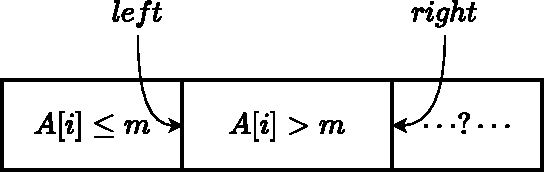
\includegraphics[scale=0.7]{img/partition-by}  % by pdfcrop
  \caption{数组划分。位于$0 \leq i < left$的元素满足$A[i] \leq m$,位于$left \leq i < right$的元素满足$A[i] > m$,剩余的元素尚未处理。}
  \label{fig:divide}
\end{figure}

\section*{正规数}

第二道趣题是如何寻找第1500个正规数。正规数是只含有2、3、5这三种因子的自然数。在数论中叫作5-光滑数。在计算机科学中又叫作哈明数以纪念理查德$\cdot$哈明。2、3、5本身也是正规数。$60 = 2^23^15^1$是第25个正规数。数字$21 = 2^03^17^1$含有因子7,所以不是正规数。定义$1=2^03^05^0$是第0个正规数。前10个正规数如下:

1, 2, 3, 4, 5, 6, 8, 9, 10, 12, ...

\subsection*{穷举法}
我们可以从1开始,逐一检查所有自然数,对每个数把2、3、5这些因子不断去掉,检查最终结果是否为1:

\begin{algorithmic}[1]
\Function{Regular-Number}{$n$}
  \State $x \gets 1$
  \While{$n > 0$}
    \State $x \gets x + 1$
    \If{\Call{Valid?}{$x$}}
      \State $n \gets n - 1$
    \EndIf
  \EndWhile
  \State \Return $x$
\EndFunction
\Statex
\Function{Valid?}{$x$}
  \While{$x \bmod 2 = 0$}
    \State $x \gets x / 2$
  \EndWhile
  \While{$x \bmod 3 = 0$}
    \State $x \gets x / 3$
  \EndWhile
  \While{$x \bmod 5 = 0$}
    \State $x \gets x / 5$
  \EndWhile
  \State \Return $x = 1$ ?
\EndFunction
\end{algorithmic}

随着$n$增大,穷举法用时迅速增加。在同样的计算机上,其C语言实现需要40.39秒才找到第1500个正规数(860934420)。

\subsection*{构造性解法}
取模和除法是耗时的计算\cite{Bentley}。如果不再检查每一个数的因子,而是从2、3、5构造正规数,这样问题就转换为如何从小到大依次产生正规数序列。我们可以使用队列来解决。队列从一侧加入元素,另一侧取出元素。先放入的先被取出。这一特性被称为先进先出FIFO(First In First Out)。先把第0个正规数1加入队列,不断从另一侧取出正规数,分别乘以2、3、5,产生3个正规数并按大小顺序将其加入队列。如果新产生的数已存在于队列中,则丢弃以避免重复。新数可能小于队尾的数,在插入时需要保持它们的大小顺序,如\cref{fig:queues}所示。

\begin{figure}[htbp]
  \centering
  \subcaptionbox{1入队}{\includegraphics[scale=0.5]{img/q1}}
  \hspace{.1\textwidth}
  \subcaptionbox{2、3、5入队}{\includegraphics[scale=0.5]{img/q2}}
  \\
  \subcaptionbox{4、6、10入队}{\includegraphics[scale=0.5]{img/q3}}
  \hspace{.1\textwidth}
  \subcaptionbox{9、15入队,丢弃6}{\includegraphics[scale=0.5]{img/q4}}
  \caption{前4步}
  \label{fig:queues}
\end{figure}

根据这一思路的实现如下:

\begin{algorithmic}[1]
\Function{Regular-Number}{$n$}
  \State $Q \gets [1]$
  \While{$n > 0$}
    \State $x \gets$ \Call{Dequeue}{$Q$}
    \State \Call{Unique-Enqueue}{$Q, 2x$}
    \State \Call{Unique-Enqueue}{$Q, 3x$}
    \State \Call{Unique-Enqueue}{$Q, 5x$}
    \State $n \gets n-1$
  \EndWhile
  \State \Return $x$
\EndFunction
\Statex
\Function{Unique-Enqueue}{$Q, x$}
  \State $i \gets 0, m \gets |Q|$
  \While{$i < m$ 且 $Q[i] < x$}
    \State $i \gets i + 1$
  \EndWhile
  \If{$i \geq m$ 或 $x \neq Q[i]$}
    \State \Call{Insert}{$Q, i, x$}
  \EndIf
\EndFunction
\end{algorithmic}

对于长度为$m$的队列,\textproc{Unique-Enqueue}需要$O(m)$时间按序、无重复地插入新元素。队列的长度随着$n$线性增加(每取出一个后最多插入三个新元素,增加的比率$\leq 2$),总运行时间为$O(1 + 2 + 3 + ... + n) = O(n^2)$。\Cref{fig:big-O-1q}显示了队列的访问次数和$n$之间的关系,形状为二次曲线,反映出$O(n^2)$的复杂度。

\begin{figure}[htbp]
  \centering
  \includegraphics[scale=0.5]{img/big-O-1q}
  \caption{队列访问次数和$n$的关系}
  \label{fig:big-O-1q}
\end{figure}

在同样的计算机上,其C语言实现仅用0.016秒就输出了答案,比穷举法快2500倍。我们也可以用递归实现,令$xs$为包含所有正规数的无穷序列$[x_1, x_2, x_3, ...]$。对每个正规数,将其乘以2得到的仍然是无穷正规数列:$[2x_1, 2x_2, 2x_3, ...]$。同样依次乘以3、5会得到另外两个无穷正规数列。如果将这3个无穷数列合并,去除重复并将1添加到开头,就又得到了$xs$:

\be
  xs = 1 : [2x | x \gets xs] \cup [3x | x \gets xs] \cup [5x | x \gets xs]
\ee

其中$x \cons xs$表示将元素$x$连接到列表$xs$的前面,在Lisp中这个操作称为cons。1是第0个正规数,在最前面。$\cup$合并无穷列表。

\[
(a \cons as) \cup (b \cons bs) = \begin{cases}
  a < b: & a : as \cup (b \cons bs) \\
  a = b: & a : as \cup bs \\
  a > b: & b : (a \cons as) \cup bs \\
\end{cases}
\]

对应的Haskell例子程序:
\begin{Haskell}
xs = 1 : (map (*2) xs) `merge` (map (*3) xs) `merge` (map (*5) xs)

merge (a:as) (b:bs) | a < b = a : merge as (b:bs)
                    | a == b = a : merge as bs
                    | otherwise = b : merge (a:as) bs
\end{Haskell}

通过\texttt{xs !! 1500},可以得到第1500个正规数。在同样的计算机上,这一程序用时0.03秒。

\subsection*{队列}
上面的解法需要排除掉重复元素、扫描队列以保持有序。把所有正规数分成三个类:$Q_2 = \{2^i | i > 0\}$仅包含被2整除的数;$Q_{23} = \{ 2^i3^j | i \geq 0, j > 0 \}$、$Q_{235} = \{ 2^i3^j5^k | i,j \geq 0, k > 0\}$。其中$Q_{23}$要求$j \neq 0$,$Q_{235}$要求$k \neq 0$,保证了三类数间没有重复。每类数都用一个队列来产生。初始化$Q_2=\{ 2 \}$,$Q_{23} = \{ 3 \}$和$Q_{235} = \{ 5 \}$。每次取出三个队列头部的最小元素$x$,然后进行下面的检查:

\begin{itemize}
\item 如果$x$来自$Q_2$,将$2x$加入$Q_2$,$3x$加入$Q_{23}$,$5x$加入$Q_{235}$;
\item 如果$x$来自$Q_{23}$,将$3x$加入$Q_{23}$,$5x$加入$Q_{235}$。我们不应将$2x$加入$Q_2$,因为$Q_2$中不包含被3整除的数。
\item 如果$x$来自$Q_{235}$,将$5x$加入$Q_{235}$。我们不应将$2x$加入$Q_2$,$3x$加入$Q_{23}$,因为它们不包含被5整除的数。
\end{itemize}

不断从三个队列中取出最小的直到第$n$个元素。\cref{fig:q235}给出了前4步。

\begin{figure}[htbp]
  \centering
  \subcaptionbox{4、6、10入队}{\includegraphics[scale=0.5]{img/q235-1}}
  \subcaptionbox{9、15入队}{\includegraphics[scale=0.5]{img/q235-2}} \\
  \subcaptionbox{8、12、20入队}{\includegraphics[scale=0.5]{img/q235-3}} \\
  \subcaptionbox{25入队}{\includegraphics[scale=0.5]{img/q235-4}}
  \caption{使用三个队列$Q_2$、$Q_{23}$、$Q_{235}$构造正规数的前4步。}
  \label{fig:q235}
\end{figure}

\begin{algorithmic}[1]
\Function{Regular-Number}{$n$}
  \State $x \gets 1$
  \State $Q_2 \gets \{ 2 \}$, $Q_{23} \gets \{ 3 \}$, $Q_{235} \gets \{ 5 \}$
  \While{$n > 0$}
    \State $x \gets min$(\Call{Head}{$Q_2$}, \Call{Head}{$Q_{23}$}, \Call{Head}{$Q_{235}$})
    \If{$x =$ \Call{Head}{$Q_2$}}
      \State \Call{Dequeue}{$Q_2$}
      \State \Call{Enqueue}{$Q_2, 2x$}
      \State \Call{Enqueue}{$Q_{23}, 3x$}
      \State \Call{Enqueue}{$Q_{235}, 5x$}
    \ElsIf{$x=$ \Call{Head}{$Q_{23}$}}
      \State \Call{Dequeue}{$Q_{23}$}
      \State \Call{Enqueue}{$Q_{23}, 3x$}
      \State \Call{Enqueue}{$Q_{235}, 5x$}
    \Else
      \State \Call{Dequeue}{$Q_{235}$}
      \State \Call{Enqueue}{$Q_{235}, 5x$}
    \EndIf
    \State $n \gets n - 1$
  \EndWhile
  \State \Return $x$
\EndFunction
\end{algorithmic}

算法循环$n$次。每次从三个队列中取出最小元素,这一步需要常数时间。接着根据取出元素所在的队列,产生一到三个新数加入队列,这一步也是常数时间。整个算法复杂度为$O(n)$。

\section*{小结}
尽管两道趣题都能用穷举法解决,但随着规模增加,我们不得不寻求更好的解法。本书介绍常见的基本算法和数据结构,同时给出函数式和命令式的对比实现。主要参考了冈崎的著作\cite{okasaki-book}和经典的算法教材\cite{CLRS}。本书尽量避免依赖于特定的编程语言。一方面读者会有自己的偏好,另一方面编程语言也在不断变化。为此我们主要使用伪代码和数学记法对算法进行定义,并附以一些例子代码。函数式的示例类似Haskell,命令式的示例是几种语言的混合体。

本书中文版《算法新解》从2009年开始写作,2017年出版。2020年底开始重写,2022年2月完成了第二版。电子版可以在github上获得,如果希望获得纸质版,请在github上联系我。

\begin{Exercise}\label{ex:preface}
\Question{最小可用数趣题中,所有数都是非负整数。我们可以利用正负号来标记一个数字是否存在。首先扫描一遍列表,令列表长度为$n$,对于任何绝对值小于$n$的数$|x| < n$,将位置$|x|$上的数字置为负数。之后再次扫描一遍列表,找到第一个正数所在的位置就是答案。编程实现这一算法。}

\Question{$n$个数字1, 2, ..., $n$,经过某一处理后,它们的顺序被打乱了,并且某一个数$x$被改成了$y$。假设$1 \leq y \leq n$,设计一个方法能够在线性时间、常数空间内找出$x$和$y$。}

\Question{下面是一段求正规数的代码。它是一种队列解法么?
\begin{lstlisting}[language = Bourbaki]
Int regularNum(Int m) {
    [Int] nums(m + 1)
    Int n = 0, i = 0, j = 0, k = 0
    nums[0] = 1
    Int x2 = 2 * nums[i]
    Int x3 = 3 * nums[j]
    Int x5 = 5 * nums[k]
    while n < m {
        n = n + 1
        nums[n] = min(x2, x3, x5)
        if x2 == nums[n] {
            i = i + 1
            x2 = 2 * nums[i]
        }
        if x3 == nums[n] {
            j = j + 1
            x3 = 3 * nums[j]
        }
        if x5 == nums[n] {
            k = k + 1
            x5 = 5 * nums[k]
        }
    }
    return nums[m]
}
\end{lstlisting}
}
\end{Exercise}

\begin{Answer}[ref={ex:preface}]
\Question{最小可用数趣题中,所有数都是非负整数。我们可以利用正负号来标记一个数字是否存在。首先扫描一遍列表,令列表长度为$n$,对于任何绝对值小于$n$的数$|x| < n$,将位置$|x|$上的数字置为负数。之后再次扫描一遍列表,找到第一个正数所在的位置就是答案。编程实现这一算法。

\begin{Bourbaki}
Int minFree([Int] nums) {
    var n = length(nums)
    for Int i = 0 to n {
        var k = abs(nums[i])
        if k <= n then nums[k - 1] = -abs(nums[k - 1])
    }
    for Int i = 0 to n {
        if nums[i] > 0 then return i + 1
    }
    return n + 1
}
\end{Bourbaki}
}

\Question{$n$个数字1, 2, ..., $n$,经过某一处理后,它们的顺序被打乱了,并且某一个数$x$被改成了$y$。假设$1 \leq y \leq n$,设计一个方法能够在线性时间、常数空间内找出$x$和$y$。

例如$X$ = [3, 1, 3, 5, 4]中,丢失的是$x = 2$,重复的是$y = 3$。我们给出4种解法:(1)分治、(2)鸽笼排序、(3)符号编码、(4)解方程。

\textbf{分治}方法。使用中点$m = \lfloor \dfrac{1 + n}{2} \rfloor$划分序列为两部分,左侧:$as = [a \leq m, a \gets X]$、右侧:$bs = [b > m, b \gets X]$。如果左侧长度$|as| < m$,可知丢失的数字在左侧,记$s = 1 + 2 + ... + m = \dfrac{m (m + 1)}{2}$,则$x = s - sum(as)$。同时可计算出重复的数字在右侧,记$s' = (m + 1) + (m + 2) + ... + n = \dfrac{(n + m + 1)(n - m)}{2}$,则$y = sum(bs) - s'$;若左侧的长度$|as| > m$,可知重复的数字在左侧。使用同样的方法,可以算出丢失的数字$x = s' - sum(bs)$,重复的数字$y = sum(as) - s$;否则,如果左侧的长度$|as| = m$,说明有$m$个不大于$m$的数字,但我们不知道它们是否是1, 2, ..., $m$的某个排列。为此,我们可以计算并比较$sum(as)$和$s$。如果相等,说明左侧没有问题,可以丢弃左侧的所有数字,然后递归地在右侧寻找$x$和$y$;否则,我们丢弃右侧,在左侧递归寻找答案。在递归查找时,需要用序列的下限$l$替换上述步骤中的1。由于每次去掉一半的列表,根据主定理,总时间复杂度为$O(n)$。或通过等比数列推导复杂度:$O(n + n/2 + n/4 + ...) = O(2n) = O(n)$。

\begin{Haskell}
missDup xs = solve xs 1 (length xs) where
  solve xs@(_:_:_) l u | k < m - l + 1 = (sl - sl', sr' - sr)
                       | k > m - l + 1 = (sr - sr', sl' - sl)
                       | sl == sl' = solve bs (m + 1) u
                       | otherwise = solve as l m
      where
          m = (l + u) `div` 2
          (as, bs) = partition (<=m) xs
          k = length as
          sl = (l + m) * (m - l + 1) `div` 2
          sr = (m + 1 + u) * (u - m) `div` 2
          (sl', sr') = (sum as, sum bs)
\end{Haskell}

\textbf{鸽笼排序}。由于所有的数字都在1到$n$之间,我们可以使用鸽笼排序来重新排列数字。我们自左向右扫描,对于每个位置$i$上的数字$x$,如果$x \neq i$,我们就将它和位置$x$上的数字$y$交换。如果$x = y$,我们就找到了重复的数字,同时,我们得知丢失的数字就是$i$,重复这一交换过程,直到$x$等于$i$或者找到重复的数字。由于每个数字仅被交换一次以到达正确的位置,因此总时间复杂度为$O(n)$。

\begin{Bourbaki}
(Int, Int) missDup([Int] xs) {
    (Int miss, Int dup) = (-1, -1)
    for Int i = 0 to length(xs) - 1 {
        while xs[i] != i {
            Int j = xs[i]
            if xs[j] == xs[i] {
                dup = xs[j]
                miss = i
                break
            } else {
                j = xs[i]
                (xs[i], xs[j]) = (xs[j], xs[i])
            }
        }
    }
    return (miss, dup)
\end{Bourbaki}

\textbf{符号编码}。假设存在一个长度为$n$的标记数组,对于序列中的每个数字$x$,我们都将标记数组中的第$x$个位置做上标记。当我们遇到重复元素时,我们会发现这个位置上的标记已经做过了。记重复的数字为$d$,我们知道$s = 1 + 2 + ... + n = \dfrac{n (n + 1)}{2}$,以及序列中所有的数字和$s'$。我们可以计算出丢失的数字$m = d + s - s'$。 但是这一方法需要额外长度为$n$的空间用作标记数组。由于数字的存在与否是一种二值化的信息(有、无),我们可以将其编码为数字的正负号,从而复用待查找的数字序列。对于序列中的每个数字$x$,我们将序列中第$|x|$位置上的元素标记为负数,其中$|x|$表示$x$的绝对值。如果发现某一位置已经为负了,我们就找到了重复的元素,接下来我们就可以计算出丢失的数字。

\begin{Bourbaki}
(Int, Int) missDup([Int] xs) {
    (Int miss, Int dup) = (-1, -1)
    Int n = length(xs)
    Int s = sum(xs)
    for i = 0 to n - 1 {
        Int j = abs(xs[i]) - 1
        if xs[j] < 0 {
            dup = j
            miss = dup + n * (n + 1) / 2 - s
            break
        }
        xs[j] = - abs(xs[j])
    }
    return (miss, dup)
\end{Bourbaki}

\textbf{解方程}。考虑一个简化的问题:给定一个从1到$n$的列表,去掉一个元素,然后打乱序列的顺序,怎样能够快速找出去掉的元素呢?我们可以将列表中所有的元素相加,然后从$\dfrac{n (n + 1)}{2}$减去这一结果就得出了答案。这一思路可以表示为如下方程:

\[
m = s - s'
\]

其中$m$表示丢失的数字,$s$是从1到$n$的累加和,$s'$是列表中所有元素的和。但是同时存在丢失的元素和重复的元素,无法仅用一个方程求出两个未知数。

\be
\sum (x[i] - i) = d - m
\label{eq:miss-dup-1}
\ee

其中左侧是列表中第$i$个元素减去$i$后的累加和。能否找出第二个独立的方程呢?思路是使用平方。如果我们将第$i$个元素的平方减去$i$的平方,然后将结果累加起来。就可以得到下面的结果:

\be
\sum (x[i]^2 - i^2) = d^2 - m^2 = (d + m)(d - m)
\label{eq:miss-dup-2}
\ee

由于$d - m$不等于0,我们可以用式(\cref{eq:miss-dup-1})除以式(\cref{eq:miss-dup-2})两侧,得到另一个方程:

\be
\sum (x[i]^2 - i^2) / \sum (x[i] - i) = d + m
\label{eq:miss-dup-3}
\ee

比较方程(\cref{eq:miss-dup-1})和方程(\cref{eq:miss-dup-3}),两个方程、两个未知数,这样就可以得到结果:

\[
\begin{cases}
m = \dfrac{1}{2} (\dfrac{\sum (x[i]^2 - i^2)}{\sum (x[i] - i)} - \sum (x[i] - i)) \\
d = \dfrac{1}{2} (\dfrac{\sum (x[i]^2 - i^2)}{\sum (x[i] - i)} + \sum (x[i] - i)) \\
\end{cases}
\]

\begin{Haskell}
missDup xs = ((b `div` a - a) `div` 2, (b `div` a + a) `div` 2) where
  ys = zip xs [1..]
  a = sum [x - y | (x, y) <- ys]
  b = sum [x^2 - y^2 | (x, y) <- ys]
\end{Haskell}
}

\Question{是的,它是一种等价的队列解法。}
\end{Answer}

\ifx\wholebook\relax \else
\section*{参考答案}
\shipoutAnswer

\begin{thebibliography}{99}

\bibitem{fp-pearls}
Richard Bird. ``Pearls of functional algorithm design''. Cambridge University Press; 1 edition (November 1, 2010). ISBN-10: 0521513383. pp1 - pp6.

\bibitem{Bentley}
Jon Bentley. ``Programming Pearls(2nd Edition)''. Addison-Wesley Professional; 2 edition (October 7, 1999). ISBN-13: 978-0201657883 (中文版:《编程珠玑》)

\bibitem{okasaki-book}
Chris Okasaki. ``Purely Functional Data Structures''. Cambridge university press, (July 1, 1999), ISBN-13: 978-0521663502

\bibitem{CLRS}
Thomas H. Cormen, Charles E. Leiserson, Ronald L. Rivest and Clifford Stein. ``Introduction to Algorithms, Second Edition''. The MIT Press, 2001. ISBN: 0262032937. (中文版:《算法导论》)

\end{thebibliography}

\expandafter\enddocument
\fi


\part{树}
\ifx\wholebook\relax \else

\documentclass[b5paper]{ctexart}
\usepackage[nomarginpar
  %, margin=.5in
]{geometry}

\addtolength{\oddsidemargin}{-0.05in}
\addtolength{\evensidemargin}{-0.05in}
\addtolength{\textwidth}{0.1in}

\usepackage[cn]{../../../prelude}

\setcounter{page}{1}

\begin{document}

%--------------------------

\title{二叉搜索树}

\author{刘新宇
\thanks{{\bfseries 刘新宇} \newline
  Email: liuxinyu95@gmail.com \newline}
  }

\maketitle
\fi

\markboth{二叉搜索树}{初等算法}

\ifx\wholebook\relax
\chapter{二叉搜索树}
\numberwithin{Exercise}{chapter}
\fi

% ================================================================
%                 Introduction
% ================================================================
%\section{简介}

数组和链表通常被认为是最基础的数据结构,其实它们并不简单。在某些系统中,数组是最基本的组件,甚至链表也可以由数组来实现(第10.3节\cite{CLRS})。另一方面,在函数式环境中,链表被作为最基本的组件来实现数组和其它更复杂的数据结构。

我们选择二叉搜索树作为数据结构中的“hello world”。乔$\cdot$本特利(Jon Bentley)在《编程珠玑》\cite{Bentley}一书中,讨论了如何统计一段文字中各单词出现的次数。下面的例子程序给出了一个解法。\index{统计单词}

\lstset{language=C++, frame=single}
\begin{lstlisting}
int main(int, char**) {
    map<string, int> dict;
    string s;
    while (cin >> s)
        ++dict[s];
    for (auto it = dict.begin(); it != dict.end(); ++it)
        cout << it->first << ": " << it->second << "\n";
}
\end{lstlisting}

我们可以运行下面的命令进行统计:

\begin{verbatim}
$ cat bbe.txt | ./wordcount > wc.txt
\end{verbatim}

这里的\texttt{map}是一种用平衡二叉树实现的字典数据结构。我们用单词作为key,用单词出现的次数作为值。这个程序运行快速,展示了二叉搜索树的强大功能。在详细介绍之前,我们先来了解一下二叉树。

\section{定义}
\label{introduction} \index{二叉搜索树}

\index{二叉树}
二叉树是一种递归的数据结构,一棵二叉树:

\begin{itemize}
\item 或者为空,
\item 或者包含三个部分:一个元素和左右两个分支,这两个分支也都是二叉树。
\end{itemize}

左右分支也被称为左子树和右子树,或统称为孩子。我们也可以说一棵树由若干节点构成。节点中的值可以是任何类型或为空。如果一个节点的左右子树都为空,我们称之为叶子节点,否则称为分支节点。

\begin{figure}[htbp]
  \centering
  \subcaptionbox{二叉树的结构}{\includegraphics[scale=0.5]{img/lvr.ps}} \\
  \subcaptionbox{一棵二叉树}{\includegraphics[scale=0.5]{img/btexample.ps}}
  \caption{二叉树的结构和例子}
  \label{fig:binary-tree-example}
\end{figure}

二叉搜索树是一种特殊的二叉树,它的值可以进行比较\footnote{广义的可比较,例如大小,先后、包含等序关系。本章中的“小于”及其符号$<$是抽象的比较。},并且满足下面的条件:
\begin{itemize}
\item 对于任何节点,所有左侧分支的值都小于本节点的值,
\item 本节点的值小于所有右侧分支的值。
\end{itemize}

图\ref{fig:bst-example}展示了一棵二叉搜索树。和图\ref{fig:binary-tree-example}比较,可以看到节点组织方式的不同。一棵二叉树的值可以是任意类型,而二叉搜索树要求它的值必须能进行比较\footnote{只要能进行抽象的“小于”和“等于”比较就足够了。}。为了强调这种区别,我们特别称二叉搜索树的的值为键(key),把节点存储的其他数据信息称为值(value)。

\begin{figure}[htbp]
  \centering
  \includegraphics[scale=0.4]{img/bst-1.ps}
  \caption{二叉搜索树的例子} \label{fig:bst-example}
\end{figure}


% ================================================================
% Data layout
% ================================================================
\section{数据组织}
\index{二叉搜索树!数据组织}

根据二叉搜索树的定义,我们可以用图\ref{fig:node-layout-parent。}来描绘数据的组织结构。一个节点包含一个键和一些可选的额外数据。接下来是两个指向左右子树的两个引用。为了方便地从一个节点上溯到祖先,也可以存储一个指向父节点的引用。

\begin{figure}[htbp]
  \centering
  \includegraphics[scale=0.7]{img/node-layout-parent.ps}
  \caption{带有父节点引用的数据组织} \label{fig:node-layout-parent}
\end{figure}

简单起见,我们会忽略额外的存储数据。本章附录给出了一个例子定义。在函数式环境中,一般不使用引用或指针来进行回溯,而通常以自顶向下的递归来设计算法。以下是一个函数式的定义:

\begin{Haskell}
data Tree a = Empty
            | Node (Tree a) a (Tree a)
\end{Haskell}

% ================================================================
% Insert
% ================================================================
\section{插入}
\index{二叉搜索树!插入}

当向二叉搜索树插入一个键$k$(和相关的数据)时,我们需要确保树中的元素仍然是有序的。为此,我们可以设计如下的插入策略:

\begin{itemize}
\item 如果树为空,创建一个元素为$k$的叶子节点;
\item 如果$k$小于根节点中的元素,将它插入到左子树中;
\item 否则,将$k$插入到右子树中。
\end{itemize}

这里存在一个特殊情况:当$k$等于根节点中的元素时,说明它已经存在了。我们可以覆盖掉以前的数据,或者把新数据添加在后面,也可以跳过不做任何处理。简单起见,我们忽略这一情况。插入算法是递归的,它十分简单。可以定义为如下的函数:

\be
\begin{array}{rcl}
insert(\nil, k) & = & Node(\nil, k, \nil) \\
insert(Node(T_l, k, T_r), k) & = & \begin{cases}
  k < k': & Node(insert(T_l, k), k', T_r) \\
  otherwise: & Node(T_l, k', insert(T_r, k)) \\
  \end{cases}
\end{array}
\ee

当节点不为空时,$T_l$、$T_r$、$k'$分别是它的左右子树和键。函数$Node(l, k, r)$用左右子树和键来构造一个节点。符号$\nil$表示空或NIL。它是大数学家安德烈$\cdot$韦伊引入的挪威语字母,用来表示空集。下面是相应的例子程序:

\begin{Haskell}
insert Empty k = Node Empty k Empty
insert (Node l x r) k | k < x = Node (insert l k) x r
                      | otherwise = Node l x (insert r k)
\end{Haskell}

这一例子程序使用了模式匹配(pattern matching)特性。本章附录给出了另一个不使用此特性的例子。插入算法也可以不使用递归,而纯用迭代实现:

\begin{algorithmic}[1]
\Function{Insert}{$T, k$}
  \State $root \gets T$
  \State $x \gets$ \Call{Create-Leaf}{$k$}
  \State $parent \gets$ NIL
  \While{$T \neq$ NIL}
    \State $parent \gets T$
    \If{$k <$ \Call{Key}{$T$}}
      \State $T \gets $ \Call{Left}{$T$}
    \Else
      \State $T \gets $ \Call{Right}{$T$}
    \EndIf
  \EndWhile
  \State \Call{Parent}{$x$} $\gets parent$
  \If{$parent = $ NIL} \Comment{$T$为空}
    \State \Return $x$
  \ElsIf{$k <$ \Call{Key}{$parent$}}
    \State \Call{Left}{$parent$} $\gets x$
  \Else
    \State \Call{Right}{$parent$} $\gets x$
  \EndIf
  \State \Return $root$
\EndFunction
\Statex
\Function{Create-Leaf}{k}
  \State $x \gets $ \Call{Empty-Node}{}
  \State \Call{Key}{$x$} $ \gets k$
  \State \Call{Left}{$x$} $ \gets $ NIL
  \State \Call{Right}{$x$} $ \gets $ NIL
  \State \Call{Parent}{$x$} $ \gets $ NIL
  \State \Return $x$
\EndFunction
\end{algorithmic}

这一实现虽然没有函数式算法简洁,但执行速度更快,并且可以处理深度很大的树。

\section{遍历}
\index{二叉树!遍历}

遍历是指依次访问二叉树中的每个元素。有三种遍历方法,分别是前序遍历、中序遍历、后序遍历。它们是按照访问根节点和子节点的先后顺序命名的。

\begin{itemize}
\item 前序遍历:先访问\textbf{根节点},然后访问左子树,最后访问右子树;
\item 中序遍历:先访问左子树,然后访问\textbf{根节点},最后访问右子树;
\item 后序遍历:先访问左子树,然后访问右子树,最后访问\textbf{根节点}。
\end{itemize}

\index{前序遍历} \index{中序遍历} \index{后序遍历}

所有的“访问”操作都是递归的。\textbf{先}访问根后访问子分支称为\textbf{先序},在访问左右分支的\textbf{中间}访问根称为\textbf{中序},先访问子分支\textbf{后}访问根称为\textbf{后序}。
对于图\ref{fig:bst-example}中的二叉树,三种遍历的结果分别如下:

\begin{itemize}
\item 前序遍历:4, 3, 1, 2, 8, 7, 16, 10, 9, 14
\item 中序遍历:1, 2, 3, 4, 7, 8, 9, 10, 14, 16
\item 后序遍历:2, 1, 3, 7, 9, 14, 10, 16, 8, 4
\end{itemize}

特别地,中序遍历会按照从小到大的顺序输出元素。二叉搜索树的定义保证了这一性质。我们把相应的证明留作练习。中序遍历的算法可以描述为:

\begin{itemize}
\item 如果树为空,返回;
\item 否则先中序遍历左子树,然后访问根节点,最后再中序遍历右子树。
\end{itemize}

这一描述本身是递归的。我们可以进一步定义一个$map$函数,按照中序遍历的顺序将函数$f$应用的每个元素上,从而映射成另一棵同构的树。

\be
\begin{array}{rcl}
map(f, \nil) & = & \nil \\
map(f, Node(T_l, k, T_r)) & = & Node(map(f, T_l), f(k), map(f, T_r))
\end{array}
\ee

如果只访问并操作节点上的值,而无需创建另外一棵树,我们可以将这一算法实现如下:

\begin{algorithmic}[1]
\Function{In-Order-Traverse}{$T, f$}
  \If{$T \neq$ NIL}
    \State \textproc{In-Order-Traverse}(\Call{Left}{$T, f$})
    \State $f$(\Call{Key}{$T$})
    \State \textproc{In-Order-Traverse}(\Call{Right}{$T, f$})
  \EndIf
\EndFunction
\end{algorithmic}

我们也可以修改$map$函数,通过中序遍历将一棵二叉搜索树转化为一个有序序列:

\be
\begin{array}{rcl}
toList(\nil) & = & [\ ] \\
toList(Node(T_l, k, T_r)) & = & toList(T_l) \doubleplus [ k ] \doubleplus toList(T_r) \\
\end{array}
\ee

我们据此可以得到一个排序的方法:先把一个无序的列表转化为一个二叉搜索树,然后再用中序遍历把树转换回列表。该方法被称为“树排序”。记待排序列表为$X = [x_1, x_2, x_3, ..., x_n]$。

\be
  sort(X) = toList(fromList(X))
\ee

我们也可以写成函数组合\cite{func-composition}的形式:

\[
  sort = toList \circ fromList
\]

其中函数$fromList$不断地将元素从列表中插入到一棵树中,它可以递归地定义如下:

\[
\begin{array}{rcl}
fromList([\ ]) & = & \nil \\
fromList(X) & = & insert(fromList(X'), x_1) \\
\end{array}
\]

如果列表为空,则产生的树也是空;否则它把第一个元素$x_1$插入树中,然后递归地插入剩余元素$X' = [x_2, x_3, ..., x_n]$。通过使用列表叠加\cite{wiki-fold}(详见附录A.6),我们也可以将$fromList$定义为:

\be
  fromList(X)= \fold_l(insert, \nil, X)
\ee

我们也可以进一步把它简写为柯里化的形式\cite{curry}(也称为部分应用)从而省略掉参数$X$:

\[
  fromList = \fold_l\ insert\ \nil
\]

\begin{Exercise}
\Question{给定如下前序遍历和中序遍历的结果,请重建出二叉树,并给出后序遍历的结果。
\begin{itemize}
\item 前序遍历结果:1, 2, 4, 3, 5, 6
\item 中序遍历结果:4, 2, 1, 5, 3, 6
\item 后序遍历结果:?
\end{itemize}
\index{重建树}
}

\Question{归纳前一题的规律,编程实现从前序遍历和中序遍历的结果重建二叉树。}

\Question{证明对二叉搜索树进行中序遍历可以将全部元素按照从小到大的顺序输出。}

\Question{对于$n$个元素,树排序的算法复杂度是什么?}
\end{Exercise}

% ================================================================
% Querying a binary search tree
% ================================================================
\section{搜索}
\index{二叉搜索树!搜索}
\index{二叉搜索树!查找}

由于二叉搜索树中的元素是按序递归存储的,它可以方便地支持各种搜索。这也是人们将其命名为“搜索树”的原因。有三种不同类型的搜索:1)在树中查找一个键;2)寻找最大或最小元素;3)查找某一元素的前驱(上一个)或后继(下一个)元素。

\subsection{查找}
二叉搜索树的定义使得它非常适合自顶向下的查找。可以按照下面的方法在树中查找元素$k$:

\begin{itemize}
\item 如果树为空,结束查找,$k$不存在;
\item 如果根节点元素等于$k$,结束查找。结果存储在根节点中;
\item 如果$k$小于根节点元素,在左子树中递归查找;
\item 否则,在右子树中递归查找。
\end{itemize}

我们可以定义递归的$lookup$函数来实现这一算法:

\be
\begin{array}{rcl}
lookup(\nil, x) & = & \nil \\
lookup(Node(T_l, k, T_r), x) & = & \begin{cases}
  k = x: & T \\
  x < k: & lookup(T_l, x) \\
  otherwise: & lookup(T_r, x) \\
  \end{cases}
\end{array}
\ee

这一函数返回查找到的节点,如果没有找到就返回空。我们也可以返回节点内存储的值。这时可以使用$Maybe$类型(也叫作\texttt{Optional<T>})来处理未找到的情况。例如:

\begin{Haskell}
lookup Empty _ = Nothing
lookup t@(Node l k r) x | k == x = Just k
                        | x < k = lookup l x
                        | otherwise = lookup r x
\end{Haskell}


如果二叉树很平衡,大多数中间节点都有非空的左右分支(我们将在第三章给出平衡的定义),对于$n$个元素的二叉树,搜索算法的性能为$O(\lg n)$。如果二叉树很不平衡,最坏情况下,查找的时间会退化到$O(n)$。如果记树的高度为$h$,则查找算法的性能可以表示成$O(h)$的形式。

搜索算法也可以不使用递归来实现:

\begin{algorithmic}[1]
\Function{Search}{$T, x$}
  \While{$T \neq $ NIL and \Call{Key}{$T$} $ \neq x$}
    \If{$x <$ \Call{Key}{$T$}}
      \State $T \gets $ \Call{Left}{$T$}
    \Else
      \State $T \gets $ \Call{Right}{$T$}
    \EndIf
  \EndWhile
  \State \Return $T$
\EndFunction
\end{algorithmic}

\subsection{最小和最大元素}
\index{二叉搜索树!最小元素/最大元素}

在二叉搜索树中,较小的元素总是位于左侧分支,而较大的元素总是位于右侧分支。可以利用这一特性来定位最大和最小元素。为了找到最小元素,我们可以不断向左侧前进,直到左侧分支为空。对称地,我们可以通过不断向右侧前进找到最大元素。

\be
\begin{array}{rcl}
min(Node(\nil, k, T_r)) & = & k \\
min(Node(T_l, k, T_r)) & = & min(T_l) \\
\end{array}
\ee

\be
\begin{array}{rcl}
max(Node(T_l, k, \nil)) & = & k \\
max(Node(T_l, k, T_r)) & = & max(T_r) \\
\end{array}
\ee

这两个函数的性能都是$O(h)$,其中$h$是树的高度。

\subsection{前驱和后继}
\index{二叉搜索树!前驱/后继}

有时需要把二叉搜索树当作通用容器,使用迭代器进行遍历。例如从最小的元素开始,逐一向前移动到最大元素,或者按需先后移动。下面的例子程序升序输出树中的元素:

\lstset{language=Bourbaki}
\begin{lstlisting}
void printTree (Node<T> t) {
    for (var it = Iterator(t), it.hasNext(); it = it.next()) {
        print(it.get(), ", ");
    }
}
\end{lstlisting}

这就需要查找一个给定节点的前驱或后继元素。$x$的后继定义为全部满足$x < y$中的最小的一个$y$。如果$x$的右子树不为空,则右子树中的最小值就是后继。图\ref{fig:bst-succ}中8的后继元素为9,它是8的右子树中的最小值。如果$x$的右子树为空,我们需要向上回溯,找到最近的一个祖先,使得该祖先的左子树也是$x$的祖先。在图\ref{fig:bst-succ}中,元素2所在的节点没有右侧分支,我们向上回溯一步找到元素1,但是1没有左侧分支,因此需要继续向上查找,这次我们到达了元素3所在的节点。而3的左子树也是2的祖先。至此,我们找到了2的后继元素3。

\begin{figure}[htbp]
  \centering
  \includegraphics[scale=0.45]{img/bst-1.ps}
  \caption{8的后继为其右侧分支的最小值9;为了获得2的后继,首先向上找到1,它没有左子树,所以继续向上找到3,3的左子树也是2的祖先,故而后继为3。} \label{fig:bst-succ}
\end{figure}

如果沿着父节点引用一直回溯到了根节点,但是仍然没有找到位于右侧的祖先,这说明$x$没有后继(它是树中最后一个元素)。下面的算法实现了后继的查找:

\begin{algorithmic}[1]
\Function{Succ}{$x$}
  \If{\Call{Right}{$x$} $\neq $ NIL}
    \State \Return \textproc{Min}(\Call{Right}{$x$})
  \Else
    \State $p \gets $ \Call{Parent}{$x$}
    \While{$p \neq $ NIL and $x =$ \Call{Right}{$p$}}
      \State $x \gets p$
      \State $p \gets $ \Call{Parent}{$p$}
    \EndWhile
    \State \Return $p$
  \EndIf
\EndFunction
\end{algorithmic}

当$x$没有后继时,这一算法返回NIL。寻找前驱元素的算法与此对称:

\begin{algorithmic}[1]
\Function{Pred}{$x$}
  \If{\Call{Left}{$x$} $\neq $ NIL}
    \State \Return \textproc{Max}(\Call{Left}{$x$})
  \Else
    \State $p \gets $ \Call{Parent}{$x$}
    \While{$p \neq $ NIL and $x =$ \Call{Left}{$p$}}
      \State $x \gets p$
      \State $p \gets $ \Call{Parent}{$p$}
    \EndWhile
    \State \Return $p$
  \EndIf
\EndFunction
\end{algorithmic}

似乎很难找到纯函数式算法实现前驱和后继的查找。这主要是因为在缺少指向父节点的引用\footnote{ML或OCaml中有\texttt{ref}引用概念,这里我们限于纯函数式环境。}。一种折衷的方案是在遍历树的时候,留下一些“面包屑”作为标记。用以将来回溯甚至重建整棵树。这种同时包含树和“面包屑”信息的数据结构称为zipper(\cite{learn-haskell}最后一章)。

查找前驱和后继的初衷是“作为一个通用容器,遍历树中的全部元素”。而在纯函数式环境中,我们通常用$map$函数中序遍历所有元素。前驱和后续的查找,仅在命令式环境中才有意义。另外一个这样仅在命令式环境中才有引起关注的例子是红黑树中元素的删除\cite{okasaki-blog}。

\begin{Exercise}

\Question{使用\textproc{Pred}和\textproc{Succ}实现一个二叉搜索树的迭代器。用它遍历一棵含有$n$个元素的树的复杂度是什么?}

\Question{下面程序可以遍历一个区间$[a, b]$内的元素:

\texttt{for\_each (m.lower\_bound(12), m.upper\_bound(26), f);}

试用纯函数式的方法解决这一问题
\index{区间遍历}
}
\end{Exercise}

% ================================================================
%                 Deletion
% ================================================================
\section{删除}
\index{二叉搜索树!删除}
在二叉搜索树中删除元素需要额外的处理。我们必须保证删除后树的有序性质不能被破坏:对于任何节点,所有左侧分支的元素仍然小于节点中的元素,并且所有右侧分支的元素仍然大于节点中的元素。而删除节点会破坏这一性质。

从二叉搜索树中删除节点$x$的方法如下\cite{sgi-stl}:
\begin{itemize}
\item 如果$x$没有非空子树(叶子)或者只有一棵非空子树,直接将$x$“切下”;
\item 否则,$x$有棵非空子树,我们用其右子树中的最小值$y$替换掉$x$,然后将原先的$y$“切掉”。
\end{itemize}

这一简洁的方法利用了这样一条特性:右子树中的最小值不可能有两个非空子树。所以上面的第二种情形转化为第一种情况,因而可以直接将原最小值节点“切掉”。

图\ref{fig:del-leaf}、\ref{fig:del-1child}、\ref{fig:del-branch}描述了删除时的各种情况。

\begin{figure}[htbp]
  \centering
  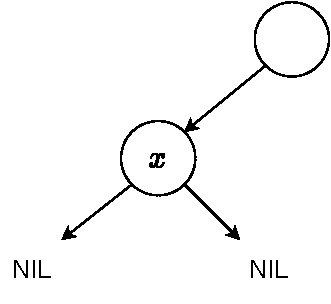
\includegraphics[scale=0.5]{img/del-leaf.ps}
  \caption{叶子节点$x$可以直接“切下”} \label{fig:del-leaf}
\end{figure}

\begin{figure}[htbp]
  \centering
  \subcaptionbox{删除$x$前}{\includegraphics[scale=0.5]{img/del-lc-before.ps}}
  \subcaptionbox{删除$x$后。$x$被“切掉”并由其左侧分支代替}{\includegraphics[scale=0.5]{img/del-lc-after.ps}} \\
  \subcaptionbox{删除$x$前}{\includegraphics[scale=0.5]{img/del-rc-before.ps}}
  \subcaptionbox{删除$x$后。$x$被“切掉”并由其右侧分支代替}{\includegraphics[scale=0.5]{img/del-rc-after.ps}}
  \caption{删除只有一个非空子分支的节点}
  \label{fig:del-1child}
\end{figure}

\begin{figure}[htbp]
  \centering
  \subcaptionbox{删除$x$前}{\includegraphics[scale=0.5]{img/del-branch-before.ps}}
  \subcaptionbox{删除$x$后。$x$被替换为右侧分支中的被“切下”的最小值}{ \includegraphics[scale=0.5]{img/del-branch-after.ps}}
  \caption{删除有两个非空分支的节点}
  \label{fig:del-branch}
\end{figure}

根据这个思路,我们定义下面的$delete$函数:

\be
\begin{array}{rcl}
delete(\nil, x) & = & \nil\\
delete(Node(T_l, k, T_r), x) & = & \begin{cases}
  x < k: & Node(delete(T_l, x), k, T_r) \\
  x > k: & Node(T_l, k, delete(T_r, x)) \\
  x = k: & del(T_l, T_r) \\
\end{cases}
\end{array}
\ee

算法先通过序关系找到待删除节点,然后调用$del$函数处理,$del$会根据情况递归调用$delete$以删除右子树中的最小值。

\be
\begin{array}{rcl}
del(\nil, T_r) & = & T_r \\
del(T_l, \nil) & = & T_l \\
del(T_l, T_r) & = & Node(T_l, y, delete(T_r, y)) \\
\end{array}
\ee

其中$y = min(T_r)$是右子树中的最小元素。下面是相应的例子程序:

\begin{Haskell}
delete Empty _ = Empty
delete (Node l k r) x | x < k = Node (delete l x) k r
                      | x > k = Node l k (delete r x)
                      | otherwise = del l r
  where
    del Empty r = r
    del l Empty = l
    del l r = let k' = min r in Node l k' (delete r k')
\end{Haskell}

如果树的高度为$h$,则删除算法的复杂度为$O(h)$。命令式算法需要在删除后,把父节点设置正确。下面的算法返回删除后树的根节点。

\begin{algorithmic}[1]
\Function{Delete}{$T, x$}
  \State $r \gets T$
  \State $x' \gets x$ \Comment{save $x$}
  \State $p \gets $ \Call{Parent}{$x$}
  \If{\Call{Left}{$x$} $= $ NIL}
    \State $x \gets $ \Call{Right}{$x$}
  \ElsIf{\Call{Right}{$x$} $= $ NIL}
    \State $x \gets $ \Call{Left}{$x$}
  \Else
    \Comment{neither children is empty}
    \State  $y \gets $ \textproc{Min}(\Call{Right}{$x$})
    \State \Call{Key}{$x$} $\gets$ \Call{Key}{$y$}
    \State Copy other satellite data from $y$ to $x$
    \If{\Call{Parent}{$y$} $\neq x$}
      \Comment{$y$ does not have left sub-tree}
      \State \textproc{Left}(\Call{Parent}{$y$}) $\gets$ \Call{Right}{$y$}
    \Else
      \Comment{$y$ is the root of the right sub-tree}
      \State \Call{Right}{$x$} $\gets$ \Call{Right}{$y$}
    \EndIf
    \If{\Call{Right}{$y$} $\neq $ NIL}
      \State \textproc{Parent}(\Call{Right}{$y$}) $\gets$ \Call{Parent}{$y$}
    \EndIf
    \State Remove $y$
    \State \Return $r$
  \EndIf
  \If{$x \neq $ NIL}
    \State \Call{Parent}{$x$} $\gets p$
  \EndIf
  \If{$p = $ NIL}
    \Comment{remove the root}
    \State $r \gets x$
  \Else
    \If{\Call{Left}{$p$} $= x'$}
      \State \Call{Left}{$p$} $\gets x$
    \Else
      \State \Call{Right}{$p$} $\gets x$
    \EndIf
  \EndIf
  \State Remove $x'$
  \State \Return $r$
\EndFunction
\end{algorithmic}

假定待删除的节点$x$不为空。算法首先记录下树的根节点、待删除的节点和它的父节点。如果$x$的任一分支为空,算法直接将$x$“切掉”。否则,如果两个子分支都不为空,我们需要先在右子树中找到最小值节点$y$。用$y$替换掉$x$中的值,同时将附加数据也替换过去。最后将原先的$y$“切掉”。我们还需要处理$y$是$x$右子树的根节点这一特殊情况。

此后还需要把之前保存的父节点重新设好。如果父节点为空,则说明要删除的节点是根节点。这种情况下,我们需要返回新的根。当父节点被设置好后,就可以安全把$x$删除了。对于高度为$h$的树,这一算法的复杂度也是$O(h)$。

\begin{Exercise}
\Question{当节点的两个分支都不为空时,存在一种对称的删除算法:用左子树的最大值替换待删除的节点,然后将此最大值的节点“切下”。编程实现这一算法。}
\end{Exercise}

\section{随机构建}
\index{二叉搜索树!随机构建}

本章给出的所有算法的复杂度都依赖于树的高度$h$。如果树非常不平衡,$O(h)$就会接近$O(n)$,因而退化为线性复杂度。反之,如果树平衡,$O(h)$接近$O(\lg n)$,算法的性能就会很好。

第三、四章将介绍两种保证二叉搜索树的平衡的方法。这里我们先给出一个简单的方法(\cite{CLRS}第265-268页):可以通过随机构建来减小不平衡性。也就是说,在构建二叉搜索树前,先通过随机函数打乱元素的次序,然后再依次插入。

\begin{Exercise}
\Question{编程实现随机构建二叉搜索树。}
\Question{如何在一棵二叉树中找到“距离最远”的两个节点?}
\end{Exercise}

\section{附录:例子代码}

包含父节点引用的二叉搜索树的例子定义:

\lstset{language=Bourbaki, frame=single}
\begin{lstlisting}
data Node<T> {
    T key
    Node<T> left
    Node<T> right
    Node<T> parent

    Node(T x) { key = x }
    Node(Node<T> l, T k, Node<T> r) {
        left = l, key = k, right = r
    }
}
\end{lstlisting}

不使用模式匹配的插入算法:

\begin{lstlisting}
Node<T> insert (Node<T> t, T x) {
    if (t == null) {
        return Node(null, x, null)
    } else if (t.key < x) {
        return Node(insert(t.left, x), t.key, t.right)
    } else {
        return Node(t.left, t.key, insert(t.right, x))
    }
}
\end{lstlisting}

消除递归的查找算法:

\begin{lstlisting}
Optional<Node<T>> lookup (Node<T> t, T x) {
    while (t != null and t.key != x) {
        if (x < t.key) {
            t = t.left
        } else {
            t = t.right
        }
    }
    return Optional(t);
}
\end{lstlisting}

迭代寻找最小元素:

\begin{lstlisting}
Optional<Node<T>> min (Node<T> t) {
    while (t != null and t.left != null) {
        t = t.left
    }
    return Optional(t);
}
\end{lstlisting}

寻找给定节点的后继:

\begin{lstlisting}
Optional<Node<T>> succ (Node<T> x) {
    if (x == null) {
        return Optional.None
    } else if (x.right != null) {
        return min(x.right)
    } else {
        p = x.parent
        while (p != null and x == p.right) {
            x = p
            p = p.parent
        }
        return Optional(p);
    }
}
\end{lstlisting}

删除节点:

\begin{lstlisting}
Node<T> delete(Node<T> t, Node<T> x) {
    if (x == null) {
        return t
    }
    root, x0, parent = t, x, x.parent
    if (x.left == null) {
        x = x.right
    } else if (x.right == null) {
        x = x.left
    } else {
        y = min(x.right)
        x.key = y.key
        if (y.parent != x) {
            y.parent.left = y.right
        } else {
            x.right = y.right
        }
        if (y.right != null) {
            y.right.parent = y.parent
        }
        return root
    if (x != null) {
        x.parent = parent
    }
    if (parent == null) {
        root = x
    } else {
        if (parent.left == x0) {
            parent.left = x
        } else {
            parent.right = x
        }
    return root
}
\end{lstlisting}

\ifx\wholebook\relax \else
\begin{thebibliography}{99}

\bibitem{CLRS}
Thomas H. Cormen, Charles E. Leiserson, Ronald L. Rivest and Clifford Stein.
``Introduction to Algorithms, Second Edition''(《算法导论》中文版). ISBN:0262032937. The MIT Press. 2001

\bibitem{Bentley}
Jon Bentley. ``Programming Pearls(2nd Edition)''(《编程珠玑》中文版). Addison-Wesley Professional; 2 edition (October 7, 1999). ISBN-13: 978-0201657883

\bibitem{okasaki-blog}
Chris Okasaki. ``Ten Years of Purely Functional Data Structures''. http://okasaki.blogspot.com/2008/02/ten-years-of-purely-functional-data.html

\bibitem{sgi-stl}
SGI. ``Standard Template Library Programmer's Guide''. http://www.sgi.com/tech/stl/

\bibitem{wiki-fold}
http://en.wikipedia.org/wiki/Foldl

\bibitem{func-composition}
http://en.wikipedia.org/wiki/Function\_composition

\bibitem{curry}
http://en.wikipedia.org/wiki/Partial\_application

\bibitem{learn-haskell}
Miran Lipovaca. ``Learn You a Haskell for Great Good! A Beginner's Guide''. the last chapter. No Starch Press; 1 edition April 2011, 400 pp. ISBN: 978-1-59327-283-8

\end{thebibliography}

\end{document}
\fi


\ifx\wholebook\relax \else

\documentclass[b5paper]{ctexart}
\usepackage[nomarginpar
  %, margin=.5in
]{geometry}

\addtolength{\oddsidemargin}{-0.05in}
\addtolength{\evensidemargin}{-0.05in}
\addtolength{\textwidth}{0.1in}

\usepackage[cn]{../../prelude}

\setcounter{page}{1}

\begin{document}

\title{插入排序}

\author{刘新宇
\thanks{{\bfseries 刘新宇} \newline
  Email: liuxinyu95@gmail.com \newline}
  }

\maketitle
\fi

\markboth{插入排序}{基本算法}

\ifx\wholebook\relax
\chapter{插入排序}
\numberwithin{Exercise}{chapter}
\fi

\lstset{frame = single}
插入排序是一种简单直观的排序算法\footnote{忽略冒泡排序算法}。在第一章中,我们给出了它的简明定义:对于一组可比较的元素,我们不断从中取出元素,按序将其插入到一个列表中。由于每次插入都需要线性时间,排序的复杂度为$O(n^2)$,其中$n$是元素的个数。插入排序的性能不如一些分而治之的排序算法,例如快速排序和归并排序。尽管如此,我们仍然能在现代软件中找到插入排序的应用。在快速排序的实现中,通常在数据集较小的时候,回退到插入排序。

\section{简介}
\label{sec:isort-introduction} \index{插入排序}
扑克游戏中的抓牌环节非常形像地描述了插入排序的思想(\cite{CLRS}第15 - 19页)。考虑从一副洗好的牌中不断抓牌,并按序理好的过程。任何时候,人们手中的牌都是有序的。每当抓到一张新牌,就按照牌的点数,插入到合适的位置。如\cref{fig:hand-of-cards}所示。根据这一思路,我们可以这样实现插入排序:

\begin{figure}[htbp]
  \centering
  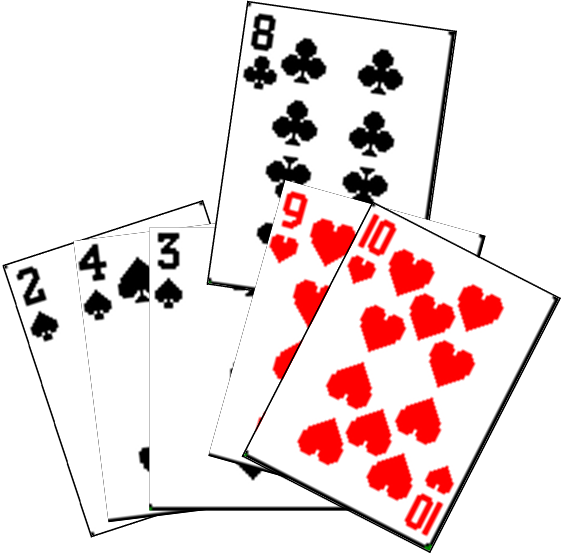
\includegraphics[scale=0.5]{img/card-deck}
  \caption{将草花8插入到一手牌中}
  \label{fig:hand-of-cards}
\end{figure}

\begin{algorithmic}[1]
\Function{Sort}{$A$}
  \State $S \gets [\ ]$
  \For{each $a \in A$}
    \State \Call{Insert}{$a, S$}
  \EndFor
  \State \Return $S$
\EndFunction
\end{algorithmic}

这一实现将排序的结果存储在新数组$S$中,也可以复用原数组的空间进行就地排序:

\begin{algorithmic}[1]
\Function{Sort}{$A$}
  \For{$i \gets 2$ to $|A|$}
    \State ordered insert $A[i]$ to $A[1...(i-1)]$
  \EndFor
\EndFunction
\end{algorithmic}

其中索引$i$的范围是从1到$n = |A|$。只含有一个元素的子数组$[A[1]]$是已序的,我们从第二个元素开始插入。当处理第$i$个元素时,所有$i$之前的元素是已序的。我们不断将未排序的元素插入,如\cref{fig:in-place-isort}所示。

\begin{figure}[htbp]
  \centering
  \includegraphics[scale=0.8]{img/in-place-sort}
  \caption{不断将元素插入已序部分}
  \label{fig:in-place-isort}
\end{figure}

\section{插入}
\index{插入排序!插入}

第一章给出了列表的插入算法。对于数组,也可以通过逐一检查找到插入位置。检查可以从左向右或者从右向左进行。下面的实现是从右向左进行检查的:

\begin{algorithmic}[1]
\Function{Sort}{$A$}
  \For{$i \gets 2$ to $|A|$}
    \Comment{Insert $A[i]$ to $A[1...(i-1)]$}
    \State $x \gets A[i]$ \Comment{将$A[i]$保存到$x$}
    \State $j \gets i-1$
    \While{$j > 0$ 且 $x < A[j]$ }
      \State $A[j+1] \gets A[j]$
      \State $j \gets j - 1$
    \EndWhile
    \State $A[j+1] \gets x$
  \EndFor
\EndFunction
\end{algorithmic}

由于数组是连续存储的,在某一位置插入元素是一个代价较高的操作。若在第$i$个位置插入元素$x$,需要把$i$后面的所有元素(包括$A[i+1]$、$A[i+2]$……)都向右移动一个位置。将第$i$个位置空出以放入$x$。如\cref{fig:array-shift}所示。

\begin{figure}[htbp]
  \centering
  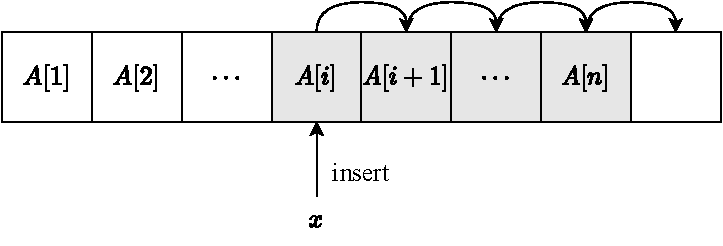
\includegraphics[scale=0.7]{img/array-shift}
  \caption{将元素$x$插入数组$A$中的第$i$个位置}
  \label{fig:array-shift}
\end{figure}

数组的长度为$n$,若比较$x$和前$i$个元素后,定位到了插入位置。接下来需要将剩余的$n - i + 1$的元素向后移动,再将$x$放入第$i$个位置。整体上看,我们相当于从左向右遍历了整个数组。另一方面,如果从右向左处理,则需要检查$n - i + 1$个元素,并执行相同数量的移动操作。我们也可以定义一个单独的\textproc{Insert}()函数,并在循环中调用。无论是从左向右或从右向左处理,插入操作都需要线性时间,因此插入排序的总体复杂度为$O(n^2)$,其中$n$是元素的个数。

\begin{Exercise}\label{ex:isort-insert}
\Question{实现从左向右处理的插入操作。}
\Question{定义单独的插入函数以实现插入排序。}
\end{Exercise}

\begin{Answer}[ref = {ex:isort-insert}]
\Question{实现从左向右处理的插入操作。
\begin{Bourbaki}
Void insert([T] xs, T x) {
    Int i = 0, n = length(xs)
    append(xs, x)
    while i < n and xs[i] < x { i++ }
    while i < n {
        xs[n] = xs[n - 1]
        n = n - 1
    }
    xs[i] = x
}
\end{Bourbaki}
}
\Question{定义单独的插入函数以实现插入排序。
\begin{Bourbaki}
Void insert([T] xs, T x) {
    append(xs, x)
    Int i = length(xs) - 1
    while i > 0 and xs[i] < xs[i-1] {
        swap(xs[i], xs[i-1])
        i--
    }
}

[T] sort([T] xs) {
    [T] ys = []
    for x in xs {
        insert(ys, x)
    }
    return ys
}
\end{Bourbaki}
}
\end{Answer}

\section{二分查找}
\index{插入排序!二分查找}

在玩扑克牌的时候,人们并不是逐一比较找到插入位置的。我们之所以能快速定位,是因为手中的牌在任何时刻都是已序的。二分查找是一种在已序序列中快速定位的方法。

\begin{algorithmic}[1]
\Function{Sort}{$A$}
  \For{$i \gets 2$ to $|A|$}
    \State $x \gets A[i]$
    \State $p \gets $ \Call{Binary-Search}{$x, A[1...(i-1)]$}
    \For{$j \gets i$ down to $p$}
      \State $A[j] \gets A[j-1]$
    \EndFor
    \State $A[p] \gets x$
  \EndFor
\EndFunction
\end{algorithmic}

二分查找时,数组中的片断$A[1...(i-1)]$是有序的。不失一般性,设其为单调增(可以定义抽象的$\leq$)。我们需要找到一个位置$j$使得$A[j-1] \leq x \leq A[j]$。我们先用$x$和中间位置的元素$A[m]$比较,其中$m = \lfloor \dfrac{i}{2} \rfloor$。如果$x < A[m]$,则递归地在前一半序列中二分查找;否则查找后一半序列。由于每次都排除掉一半元素,二分查找需要$O(\lg i)$的时间定位到插入点。

\begin{algorithmic}[1]
\Function{Binary-Search}{$x, A$}
  \State $l \gets 1, u \gets 1+|A|$
  \While{$l < u$}
    \State $m \gets \lfloor \dfrac{l+u}{2} \rfloor$
    \If{$A[m] = x$}
      \State \Return $m$ \Comment{重复元素}
    \ElsIf{$A[m] < x$}
      \State $l \gets m+1$
    \Else
      \State $u \gets m$
    \EndIf
  \EndWhile
  \State \Return $l$
\EndFunction
\end{algorithmic}

这一改进并不能提高插入排序的整体复杂度,结果仍然是$O(n^2)$。逐一比较的插入排序需要$O(n^2)$次比较和$O(n^2)$次移动;使用二分查找后,比较次数减少到了$O(n \lg n)$,但移动次数还是$O(n^2)$。

%% \begin{Exercise}
%% \Question{使用递归实现二分查找。} %见第14章,14.2 二分查找
%% \end{Exercise}

\section{列表}
\index{插入排序!列表插入排序}

二分查找将搜索时间降低到$O(n \lg n)$,但由于要依次移动数组中的元素,整体复杂度仍然是$O(n^2)$。另一方面,使用列表存储元素时,一旦获取了插入位置的引用,插入操作本身是常数时间的。在第一章中,我们定义了如下的列表插入排序算法:

\be
\begin{array}{rcl}
sort\ [\ ] & = & [\ ] \\
sort\ (x \cons xs) & = & insert\ x\ (sort\ xs) \\
\end{array}
\ee

或使用$foldr$的柯里化形式:

\be
sort = foldr\ insert\ [\ ]
\ee

由于需要遍历,列表的$insert$算法仍是线性时间的:

\be
\begin{array}{rcl}
insert\ x\ [\ ] & = & [x] \\
insert\ x\ (y \cons ys) & = & \begin{cases}
  x \leq y : & x : y : ys \\
  \text{否则}: & y : insert\ x\ ys \\
  \end{cases}
\end{array}
\ee

\label{sec:list-index-array}
也可以不使用节点引用,而通过另一个索引数组来实现列表。对任何元素$A[i]$,$Next[i]$保存了$A[i]$之后下一个元素的索引。也就是说$A[Next[i]]$是$A[i]$的下一个元素。其中有两个特殊索引:对于列表的末尾元素$A[m]$,定义$Next[m] = -1$,表示其指向NIL;此外定义$Next[0]$指向列表的头部。利用索引数组,我们定义插入算法如下:

\begin{algorithmic}[1]
\Function{Insert}{$A, Next, i$}
  \State $j \gets 0$ \Comment{$Next[0]$指向表头}
  \While{$Next[j] \neq -1$ and $A[Next[j]] < A[i]$}
    \State $j \gets Next[j]$
  \EndWhile
  \State $Next[i] \gets Next[j]$
  \State $Next[j] \gets i$
\EndFunction
\Statex
\Function{Sort}{$A$}
  \State $n \gets |A|$
  \State $Next = [1, 2, ..., n, -1]$ \Comment{$n + 1$个索引}
  \For{$i \gets 1$ to $n$}
    \State \Call{Insert}{$A, Next, i$}
  \EndFor
  \State \Return $Next$
\EndFunction
\end{algorithmic}

使用列表,尽管在引用位置进行插入只需要常数时间,但必须遍历才能找到插入位置。整体仍需要$O(n^2)$次比较。与数组不同,列表不支持随机访问,不能利用二分查找提升定位速度。

\begin{Exercise}\label{ex:list-index-array-reorder}
\Question{使用索引数组,排序结果是一个重新排列的索引。给出一个方法,根据新的索引$Next$,重新排列数组$A$。}
\end{Exercise}

\begin{Answer}[ref = {ex:list-index-array-reorder}]
\Question{使用索引数组,排序结果是一个重新排列的索引。给出一个方法,根据新的索引$Next$,重新排列数组$A$。
\begin{Bourbaki}
[K] reorder([K] xs, [Int] next) {
    Int i = -1
    [Int] ys = []
    while next[i] != -1 {
        append(ys, xs[next[i]])
        i = next[i]
    }
    return ys
}
\end{Bourbaki}
}
\end{Answer}

\section{二叉搜索树}
\index{插入排序!二叉搜索树}

我们遇到了一个困难境地:必须同时提高查找和插入的速度,仅提高其中之一仍然是$O(n^2)$的复杂度。一方面,我们希望用二分查找把比较次数降低到$O(\lg n)$;另一方面,需要改变数据结构,因为数组不支持在指定位置以常数时间插入元素。在第二章中,我们介绍了二叉搜索树。它天然就支持二分查找。一旦定位到插入位置,我们可以用常数时间插入新节点。

\begin{algorithmic}[1]
\Function{Sort}{$A$}
  \State $T \gets \nil$
  \For{each $x \in A$}
    \State $T \gets $ \Call{Insert-Tree}{$T, x$}
  \EndFor
  \State \Return \Call{To-List}{$T$}
\EndFunction
\end{algorithmic}

第二章给出了\textproc{Insert-Tree}()和\textproc{To-List}()的定义。平均情况下,树排序的复杂度为$O(n \lg n)$,其中$n$是元素的个数。这达到了基于比较的排序算法时间下限(\cite{Knuth-V3}第180-193页、\cite{CLRS}第167页)。但在最坏情况下,当树极度不平衡时,其性能会下降到$O(n^2)$。

很多情况下,插入排序常作为第一个排序算法被介绍。它简单直观,但性能是平方级别的。插入排序不仅出现在教科书中,也出现在快速排序的工程实现中:在小数据集时回退到插入排序以抵消递归的代价。

\ifx\wholebook\relax \else
\section{参考答案}
\shipoutAnswer

\begin{thebibliography}{99}

\bibitem{CLRS}
Thomas H. Cormen, Charles E. Leiserson, Ronald L. Rivest and Clifford Stein.
``Introduction to Algorithms, Second Edition''. (《算法导论》中文版)ISBN:0262032937. The MIT Press. 2001

\bibitem{Knuth-V3}
Donald E. Knuth. ``The Art of Computer Programming, Volume 3: Sorting and Searching (2nd Edition)''. Addison-Wesley Professional; 2 edition (May 4, 1998) ISBN-10: 0201896850 ISBN-13: 978-0201896855

\end{thebibliography}

\end{document}
\fi


\ifx\wholebook\relax \else
% ------------------------

\documentclass[b5paper]{ctexart}
\usepackage[nomarginpar
  %, margin=.5in
]{geometry}

\addtolength{\oddsidemargin}{-0.05in}
\addtolength{\evensidemargin}{-0.05in}
\addtolength{\textwidth}{0.1in}

\usepackage[cn]{../../../prelude}

\setcounter{page}{1}

\begin{document}

\title{红黑树}

\author{刘新宇
\thanks{{\bfseries 刘新宇} \newline
  Email: liuxinyu95@gmail.com \newline}
  }

\maketitle
\fi

\markboth{红黑树}{基本算法}

\ifx\wholebook\relax
\chapter{红黑树}
\numberwithin{Exercise}{chapter}
\fi

% ================================================================
%                 Introduction
% ================================================================
第二章的例子使用二叉搜索树来统计文章中每个词的出现次数。能否使用二叉搜索树处理通讯录,用来查询联系人的电话呢?如下面的例子代码所示:

\lstset{frame = single}
\begin{lstlisting}[language=Bourbaki]
void addrBook(Input in) {
    bst<string, string> dict
    while (string name, string addr) = read(in) {
        dict[name] = addr
    }
    loop {
        string name = read(console)
        var addr = dict[name]
        if (addr == null) {
            print("not found")
        } else {
            print("address: ", addr)
        }
    }
}
\end{lstlisting}

但这个方法性能不佳,尤其是搜索诸如Zara、Zed、Zulu等姓名时更加明显。通讯录是按照字典顺序排列的。如果依次把自然数1, 2, 3, ..., $n$插入二叉搜索树,就会得到图\ref{fig:unbalanced-tree}中的结果。这是一棵极不平衡的二叉树。对于高为$h$的二叉搜索树,查找的复杂度为$O(h)$。如果树比较平衡,我们就能够达到$O(\lg n)$的性能。但在这一极端情况下,查找的性能退化为$O(n)$。几乎等同于列表扫描。


\begin{figure}[htbp]
    \centering
	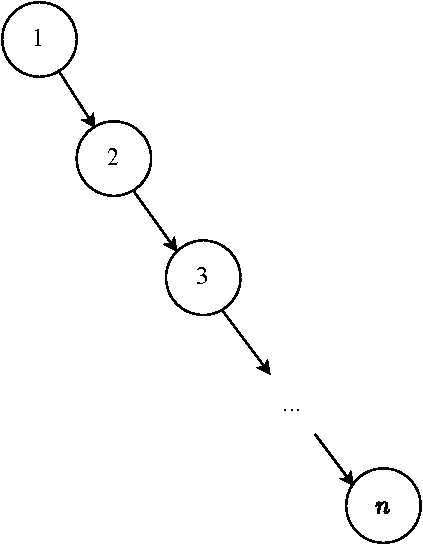
\includegraphics[scale=0.5]{img/unbalanced}
    \caption{不平衡的树} \label{fig:unbalanced-tree}
\end{figure}


\begin{Exercise}
\Question{对于较大的通讯录,为了加快构建速度,可以使用两个并发的任务:一个从头部向后,另外一个从后向前读取。当两个任务相遇时结束。这样构建出的二叉搜索树是什么样子的?如果把通讯录分成更多片断,使用多任务会得到什么结果?}
\Question{参考图\ref{fig:unbalanced-trees},找出更多的不平衡情况。}
\end{Exercise}

\begin{figure}[htbp]
  \centering
  \subcaptionbox{}{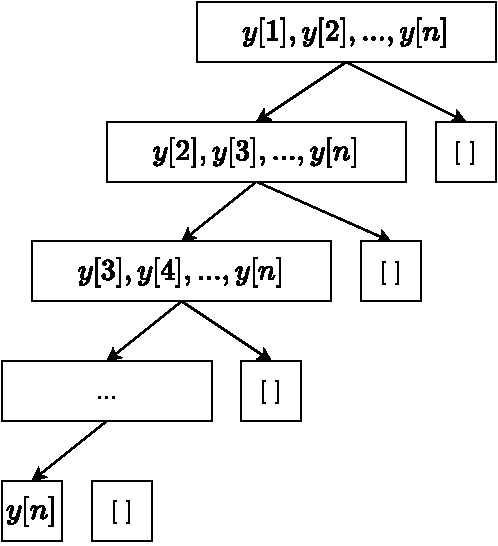
\includegraphics[scale=0.4]{img/unbalanced-2}}
  \subcaptionbox{}{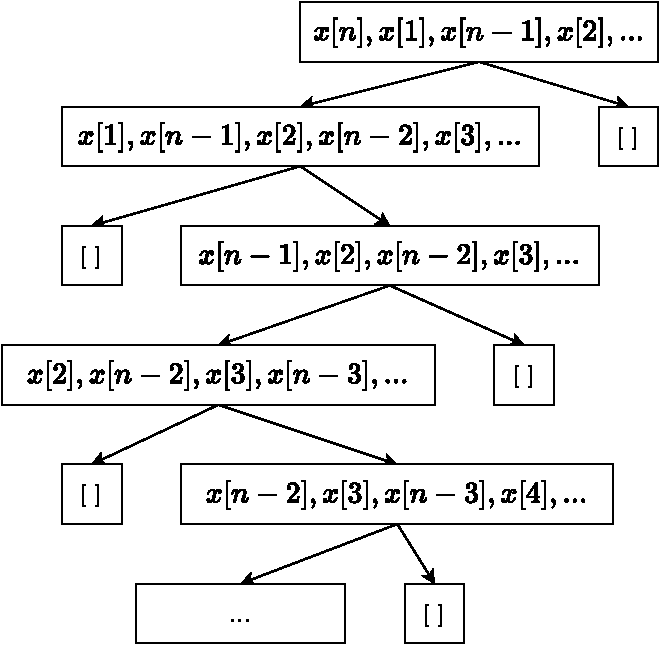
\includegraphics[scale=0.4]{img/unbalanced-zigzag}} \\
  \subcaptionbox{}{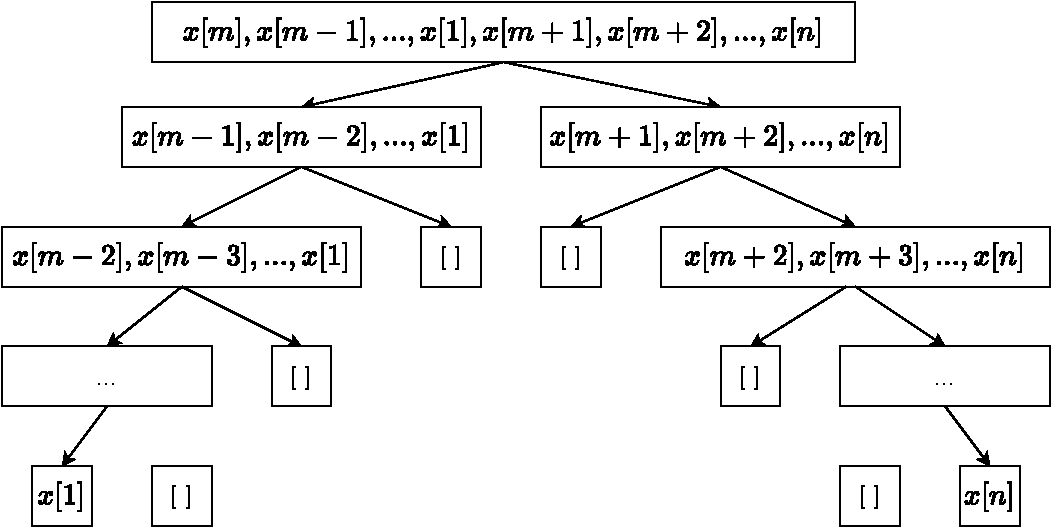
\includegraphics[scale=0.4]{img/unbalanced-3}}
  \caption{一些不平衡的二叉树}
  \label{fig:unbalanced-trees}
\end{figure}

\subsection{平衡}

为了避免这种极不平衡的情况,可以将输入序列打乱(\cite{CLRS}12.4节)。但这种方法有一定的局限性,如果序列是用户交互输入的,就无法打乱了。人们找到了一些解决平衡性的方法,它们大多依赖二叉树的旋转操作。旋转操作可以在改变树结构的同时,保持元素间顺序不变。这一章介绍红黑树。它是一种被广泛使用的自平衡二叉搜索树。下一章介绍另外一种自平衡树——AVL树。第8章还会介绍伸展树,它能够随着操作,逐步把树变得平衡。

\subsection{树旋转}
\index{树旋转}

树旋转在保持中序遍历结果不变的情况下,改变树的结构。存在多个不同的二叉树对应到一个特定的中序遍历顺序。图\ref{fig:tree-rotation}描述了旋转操作。

\begin{figure}[htbp]
  \centering
  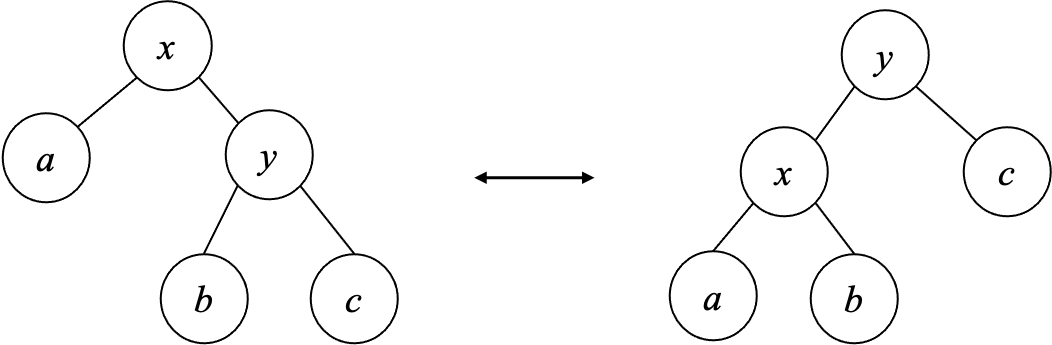
\includegraphics[scale=0.4]{img/tree-rotation}
  \caption{树的左右旋转}
  \label{fig:tree-rotation}
\end{figure}

旋转操作可以通过模式匹配来定义:

\be
\begin{array}{rcl}
rotate_l\ ((a, x, b), y, c) & = & (a, x, (b, y, c)) \\
rotate_l\ T & = & T \\
\end{array}
\ee

和

\be
\begin{array}{rcl}
rotate_r\ (a, x, (b, y, c)) & = & ((a, x, b), y, c)) \\
rotate_r\ T & = & T \\
\end{array}
\ee

如果模式没有匹配(例如两棵子树都为空),每个式子的第二行保持树不变。旋转操作也可以通过一系列步骤实现。我们需要将子树和父引用设置正确。在旋转时,我们传入根节点$T$和要旋转的子树$x$:

\begin{algorithmic}[1]
\Function{Left-Rotate}{$T, x$}
  \State $p \gets$ \Call{Parent}{$x$}
  \State $y \gets$ \Call{Right}{$x$} \Comment{设$y \ne$ NIL}
  \State $a \gets$ \Call{Left}{$x$}
  \State $b \gets$ \Call{Left}{$y$}
  \State $c \gets$ \Call{Right}{$y$}
  \State \Call{Replace}{$x, y$}  \Comment{用$y$替换$x$}
  \State \Call{Set-Subtrees}{$x, a, b$} \Comment{令$a, b$为$x$的子树}
  \State \Call{Set-Subtrees}{$y, x, c$} \Comment{令$x, c$为$y$的子树}
  \If{$p = $ NIL}  \Comment{此前$x$是根节点}
    \State $T \gets y$
  \EndIf
  \State \Return $T$
\EndFunction
\end{algorithmic}

右旋\textproc{Right-Rotate}的实现是对称的,我们将其留作练习。\textproc{Replace}($x$, $y$)使用$y$替换$x$:

\begin{algorithmic}[1]
\Function{Replace}{$x, y$}
  \State $p \gets$ \Call{Parent}{$x$}
  \If{$p$ = NIL} \Comment{$x$是根节点}
    \If{$y \ne$ NIL}
           \Call{Parent}{$y$} $\gets$ NIL
    \EndIf
  \ElsIf{\Call{Left}{$p$} $= x$}
    \State \Call{Set-Left}{$p$, $y$}
  \Else
    \State \Call{Set-Right}{$p$, $y$}
  \EndIf
  \State \Call{Parent}{$x$} $\gets$ NIL
\EndFunction
\end{algorithmic}

\textproc{Set-Subtrees}($x, L, R$)将$L$设为$x$的左子树,$R$设为右子树:

\begin{algorithmic}[1]
\Function{Set-Subtrees}{$x, L, R$}
  \State \Call{Set-Left}{$x, L$}
  \State \Call{Set-Right}{$x, R$}
\EndFunction
\end{algorithmic}

它进一步调用\textproc{Set-Left}和\textproc{Set-Right}完成子树的设置:

\begin{algorithmic}[1]
\Function{Set-Left}{$x, y$}
  \State \Call{Left}{$x$} $\gets y$
  \If{$y \ne$ NIL}
    \Call{Parent}{$y$} $\gets x$
  \EndIf
  \EndFunction

\Statex

\Function{Set-Right}{$x, y$}
  \State \Call{Right}{$x$} $\gets y$
  \If{$y \ne$ NIL}
    \Call{Parent}{$y$} $\gets x$
  \EndIf
\EndFunction
\end{algorithmic}

通过对比,可以看到模式匹配如何简化树旋转的实现。从这一点出发Okasaki在1995年实现了红黑树的纯函数式算法\cite{okasaki}。

\begin{Exercise}
\Question{实现右旋\textproc{Right-Rotate}操作。}
\end{Exercise}

\section{定义}
\index{红黑树}

红黑树是一种自平衡二叉搜索树\cite{wiki-rbt}。它是2-3-4树的等价形式\footnote{第7章,B树。对于任一2-3-4树,都存在至少一棵红黑树,其元素顺序相同。}。通过对节点进行着色和旋转,红黑树可以高效地保持平衡。我们在二叉搜索树的定义上给节点赋予红、黑颜色。我们称一棵树为红黑树,如果它满足下面5条性质\cite{CLRS}:

\index{红黑树!红黑性质}
\begin{enumerate}
\item 节点的颜色为红色或黑色。
\item 根节点为黑色。
\item 所有叶节点(NIL)为黑色。
\item 如果一个节点为红色,则它的两个子节点都是黑色。
\item 从任一节点出发到所有叶子节点的路径上包含相同数量的黑色节点。
\end{enumerate}

为什么这5条性质能保证红黑树的平衡性呢?关键在于:从根节点出发到达叶节点的所有路径中,最长路径不会超过最短路径两倍。性质4保证了不存在两个连续的红色节点。因此,最短的路径只含有黑色的节点。任何更长的路径一定含有红色节点。根据性质5,从任何节点出发的所有的路径都含有相同数量的黑色节点,自然这条对于根节点也成立。这就最终保证了没有任何路径超过最短路径长度的两倍\cite{wiki-rbt}。图\ref{fig:rbt-example-with-nil}的例子展示了一棵红黑树。

\begin{figure}[htbp]
  \centering
  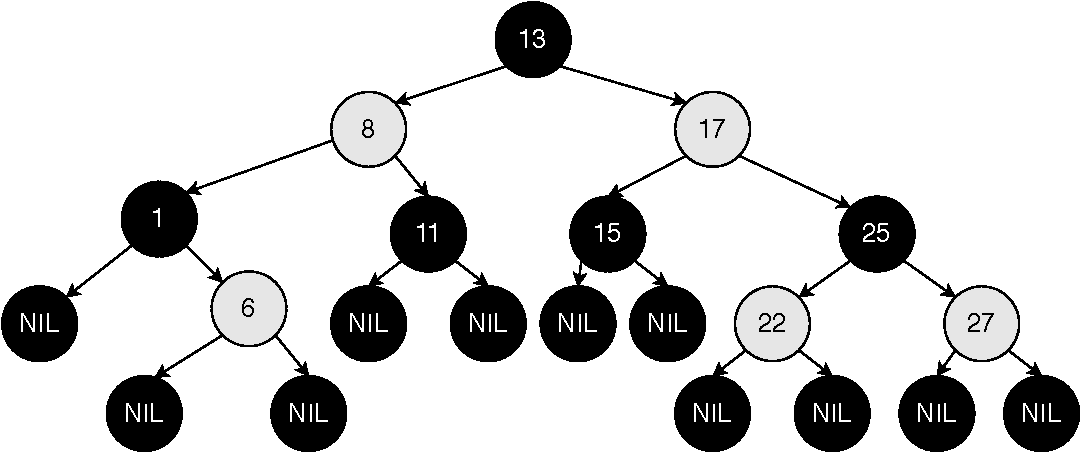
\includegraphics[scale=0.5]{img/rbt-example-with-nil}
  \caption{红黑树}
  \label{fig:rbt-example-with-nil}
\end{figure}

由于所有的NIL节点都是黑色的,我们通常将NIL节点隐藏不画出,如图\ref{fig:rbt-example-with-nil}所示。所有不改变树结构的操作都和二叉搜索树相同,包括查找、最大、最小值等。只有插入和删除操作是特殊的。

\begin{figure}[htbp]
  \centering
  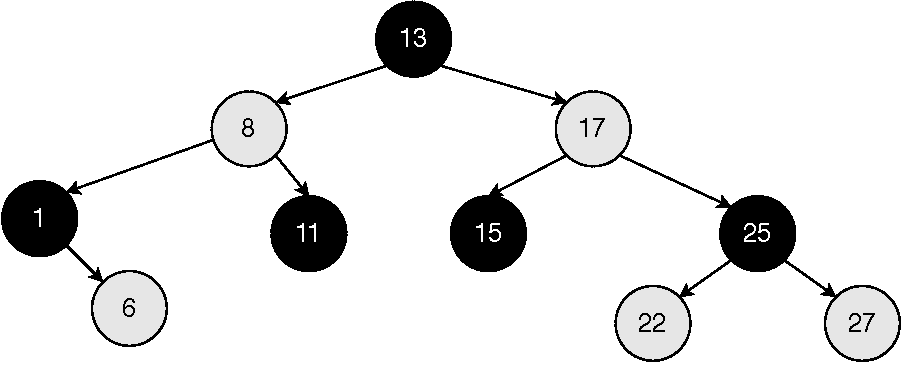
\includegraphics[scale=0.5]{img/rbt-example}
  \caption{隐藏NIL节点}
  \label{fig:rbt-example}
\end{figure}

下面的例子程序在二叉搜索树的基础上增加了颜色定义:

\begin{Haskell}
data Color = R | B
data RBTree a = Empty
              | Node Color (RBTree a) a (RBTree a)
\end{Haskell}

\begin{Exercise}
\Question{证明含有$n$个节点的红黑树,其高度$h$不会超过$2 \lg (n+1)$。}
\end{Exercise}

\section{插入}
\index{红黑树!插入}

插入算法包含两个步骤:第一步和二叉搜索树相同,树可能会变得不再平衡;第二步修复红黑树的颜色性质。插入时,我们令新节点为红色。只要它不是根节点,除了第四条外的所有性质都可以满足。唯一的问题是可能引入两个相邻的红色节点,共有4种情况需要修复。Okasaki发现它们具有统一的形式\cite{okasaki},如图 \ref{fig:insert-fix}所示。

\begin{figure}[htbp]
  \centering
  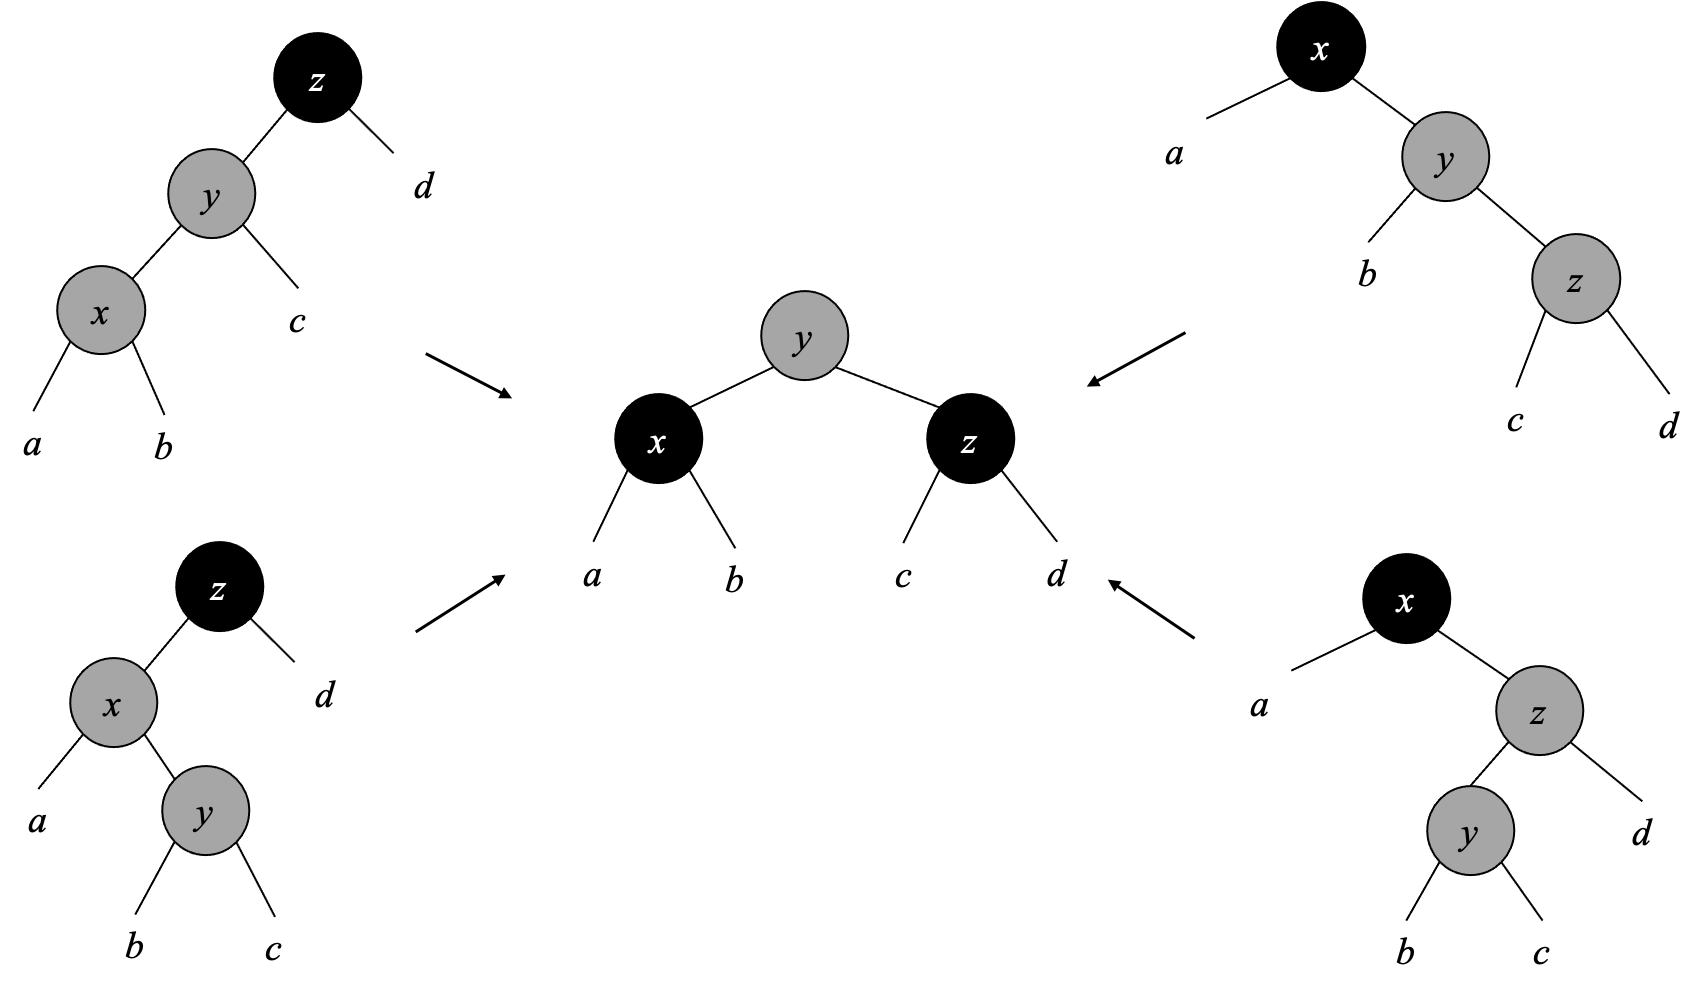
\includegraphics[scale=0.4]{img/insert-fix}
  \caption{插入后需要修复的四种情况}
  \label{fig:insert-fix}
\end{figure}

四种情况都把红色向上移动一层。如果进行自底向上的递归修复,可能会把根节点染成红色。根据性质2,最后需要把根节点变回黑色。利用模式匹配,我们定义$balance$函数修复平衡。令节点的颜色变量为$\mathcal{C}$,取值为黑色$\mathcal{B}$或红色$\mathcal{R}$。非空节点表达为一个四元组$T=(\mathcal{C}, l, k, r)$,其中$l$、$r$是左右子树,$k$是值。

\be
\begin{array}{rcl}
%\text{up left:} & & \\
balance\ \mathcal{B}\ (\mathcal{R}, (\mathcal{R}, a, x, b), y, c)\ z\ d & = & (\mathcal{R}, (\mathcal{B}, a, x, b), y, (\mathcal{B}, c, z, d)) \\
%\text{up right:} & & \\
balance\ \mathcal{B}, (\mathcal{R}, a, x, (\mathcal{R}, b, y, c))\ z\ d  & = & (\mathcal{R}, (\mathcal{B}, a, x, b), y, (\mathcal{B}, c, z, d)) \\
%\text{bottom left:} & & \\
balance\ \mathcal{B}\ a\ x\ (\mathcal{R}, b, y, (\mathcal{R}, c, z, d)) & = & (\mathcal{R}, (\mathcal{B}, a, x, b), y, (\mathcal{B}, c, z, d))  \\
%\text{bottom right:} & & \\
balance\ \mathcal{B}\ a\ x\ (\mathcal{R}, (\mathcal{R}, b, y, c), z, d) & = & (\mathcal{R}, (\mathcal{B}, a, x, b), y, (\mathcal{B}, c, z, d))  \\
%\text{otherwise:} & & \\
balance\ T & = & T \\
\end{array}
\ee

如果四种模式都不满足,最后一行保证此时不会改变树的形状。红黑树的插入算法定义如下:

\be
insert\ T\ k = makeBlack\ (ins\ T\ k)
\ee

其中

\be
\begin{array}{rcl}
ins\ \nil\ k & = & (\mathcal{R}, \nil, k, \nil) \\
ins\ (\mathcal{C}, l, k', r)\ k & = & \begin{cases}
  k < k': & balance\ \mathcal{C}\ (ins\ l\ k)\ k'\ r \\
  k > k': & balance\ \mathcal{C}\ l\ k'\ (ins\ r\ k) \\
  \end{cases}
\end{array}
\ee

如果树为空,我们为$k$创建一个红色叶子节点;否则,令树的左右分支和值分别为$l$、$r$、$k'$。比较$k$和$k'$的大小,递归地将$k$插入到子树中。然后用$balance$修复平衡性。最后强制把根节点染成黑色。

\be
makeBlack\ (\mathcal{C}, l, k, r) = (\mathcal{B}, l, k, r)
\ee

下面是对应的例子程序:

\begin{Haskell}
insert t x = makeBlack $ ins t where
    ins Empty = Node R Empty x Empty
    ins (Node color l k r)
        | x < k     = balance color (ins l) k r
        | otherwise = balance color l k (ins r)
    makeBlack(Node _ l k r) = Node B l k r

balance B (Node R (Node R a x b) y c) z d =
                Node R (Node B a x b) y (Node B c z d)
balance B (Node R a x (Node R b y c)) z d =
                Node R (Node B a x b) y (Node B c z d)
balance B a x (Node R b y (Node R c z d)) =
                Node R (Node B a x b) y (Node B c z d)
balance B a x (Node R (Node R b y c) z d) =
                Node R (Node B a x b) y (Node B c z d)
balance color l k r = Node color l k r
\end{Haskell} %$

我们略去了重复值的处理。如果要插入的值已经存在,我们可以覆盖或丢弃,还可以在节点中用一个列表存储相应的数据(\cite{CLRS},269页)。图\ref{fig:insert-example}给出了两棵红黑树。它们分别由序列11, 2, 14, 1, 7, 15, 5, 8, 4和1, 2, ..., 8构建而成。第二个例子说明,即使序列已序,红黑树仍然保持平衡。

\begin{figure}[htbp]
  \centering
  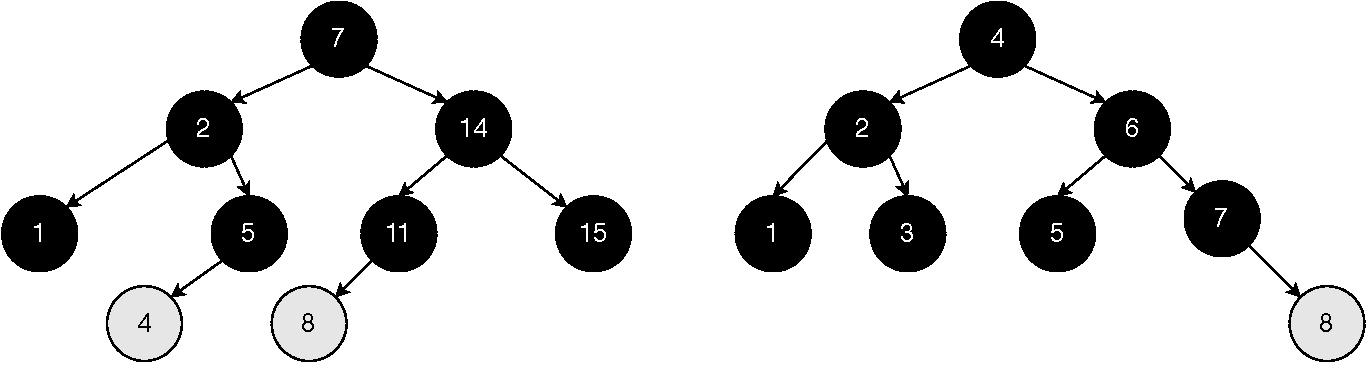
\includegraphics[scale=0.6]{img/insert-haskell}
  \caption{插入产生的红黑树}
  \label{fig:insert-example}
\end{figure}

算法自顶向下递归地进行插入和修复,对于高度为$h$的树,其复杂度为$O(h)$。由于我们始终维护红黑树的颜色性质,$h$和节点个数$n$呈对数关系。插入算法的复杂度为$O(\lg n)$。

\begin{Exercise}
\Question{不使用模式匹配,分别检查四种情况实现$insert$算法。}
\end{Exercise}

\section{删除}
\index{红黑树!删除}

红黑树的删除比插入复杂。也可以通过模式匹配和递归简化删除算法\footnote{实际上通过重用不变的部分重新构建了树。这一特性称作persist}的实现。我们还可以利用其它方式来达到删除的效果。例如,一次性构建一棵树,用于后继的多次查找\cite{okasaki-blog}。删除时在节点上加一个标记,当带有标记的节点超过50\%时,用未标记的节点重建一棵树。删除也会破坏红黑树的性质,因此同样需要进行修复。问题只发生在删除黑色节点时,这会违反性质5,使得某一路径上的黑色节点数目少于其它的路径。

我们可以引入“双重黑色”(\cite{CLRS},290页)节点来恢复第五条性质。一个这样的节点算作两个黑色节点。删除黑色节点$x$时,我们将黑色向上移动到父节点,或者向下移动到子树上。令接受黑色的节点为$y$。如果$y$原来是红色,将其变为黑色;如果$y$原来是黑色,则变为“双重黑色”,记作$\mathcal{B}^2$。下面的例子程序增加了双重黑色的定义:

\begin{Haskell}
data Color = R | B | BB
data RBTree a = Empty | BBEmpty
              | Node Color (RBTree a) a (RBTree a)
\end{Haskell}

由于所有的空节点都是黑色,当将黑色移动到空节点时,其变为“双重黑色”空节点(\texttt{BBEmpty}或加粗的$\pmb{\varnothing}$)。删除时,第一步和普通二叉搜索树相同;如果被删除节点是黑色的,接下来进行修复:

\be
delete = makeBlack \circ del
\ee

这一定义是柯里化的。如果树中只有一个元素,删除后它变为空。为了处理这一情况,我们需要修改$makeBlack$的定义如下:

\be
\begin{array}{rcl}
makeBlack\ \nil & = & \nil \\
makeBlack\ (\mathcal{C}, l, k, r) & = & (\mathcal{B}, l, k, r) \\
\end{array}
\ee

$del$接受一棵树和要删除的元素$k$:

\be
\begin{array}{rcl}
del\ \nil\ k & = & \nil \\
del\ (\mathcal{C}, l, k', r)\ k & = & \begin{cases}
  k < k': & fixB^2(\mathcal{C}, (del\ l\ k), k', r) \\
  k > k': & fixB^2(\mathcal{C}, l, k', (del\ r\ k)) \\
  k = k': & \begin{cases}
    l = \nil: & (\mathcal{C} = \mathcal{B} \mapsto shiftB\ r, r) \\
    r = \nil: & (\mathcal{C} = \mathcal{B} \mapsto shiftB\ l, l) \\
    \text{否则}: & fixB^2(\mathcal{C}, l, k'', (del\ r\ k'')) \\
    & \text{其中}\ k'' = min(r) \\
  \end{cases}
\end{cases}
\end{array}
\ee

如果树为空,结果为$\nil$;否则我们比较$k$和树中的$k'$,如果$k < k'$,我们递归地从左侧分支删除$k$;如果$k > k'$,则递归地从右侧删除。由于递归结果中可能含有双重黑色节点,需要应用$fixB^2$进行修复。当$k = k'$时,我们定位到了要删除的节点。如果任一子树为空,我们用另一子树替换掉当前节点。如果当前节点是黑色的,还需要将黑色移动到子树中。这段定义使用了麦卡锡形式$(p \mapsto a, b)$,它相当于条件表达式:(if $p$ then $a$ else $b$)。如果两棵子树都不为空,我们将右子树中的最小值$k'' = min(r)$切下,并用$k''$替换$k$。

为了保持黑色节点个数,$shiftB$将红色节点变为黑色,将黑色节点变为双重黑色。如果再次应用到双重黑色节点上,则变回黑色。

\be
\begin{array}{rcl}
shiftB\ (\mathcal{B}, l, k, r) & = & (\mathcal{B}^2, l, k, r) \\
shiftB\ (\mathcal{C}, l, k, r) & = & (\mathcal{B}, l, k, r) \\
shiftB\ \nil & = & \pmb{\nil} \\
shiftB\ \pmb{\nil} & = & \nil \\
\end{array}
\ee

下面是相应的例子程序(不包含双重黑色的修复部分):

\begin{Haskell}
delete :: (Ord a) => RBTree a -> a -> RBTree a
delete t k = makeBlack $ del t k where
    del Empty _ = Empty
    del (Node color l k' r) k
        | k < k' = fixDB color (del l k) k' r
        | k > k' = fixDB color l k' (del r k)
        | isEmpty l = if color == B then shiftBlack r else r
        | isEmpty r = if color == B then shiftBlack l else l
        | otherwise = fixDB color l k'' (del r k'') where k''= min r
    makeBlack (Node _ l k r) = Node B l k r
    makeBlack _ = Empty

shiftBlack (Node B l k r) = Node BB l k r
shiftBlack (Node _ l k r) = Node B  l k r
shiftBlack Empty = BBEmpty
shiftBlack BBEmpty = Empty
\end{Haskell}

函数$fixB^2$通过旋转操作和重新染色消除双重黑色。双重黑色节点既可能是分枝节点,也可能是空节点$\pmb{\varnothing}$。有三种情况:

\textbf{情况1:双重黑色的兄弟节点为黑色,并且该兄弟节点有一个红色子节点。}可以通过旋转修复这种情况。共有四种子情况,全部可以变换到一种统一形式。如图\ref{fig:del-case1}所示。

\begin{figure}[htbp]
   \centering
   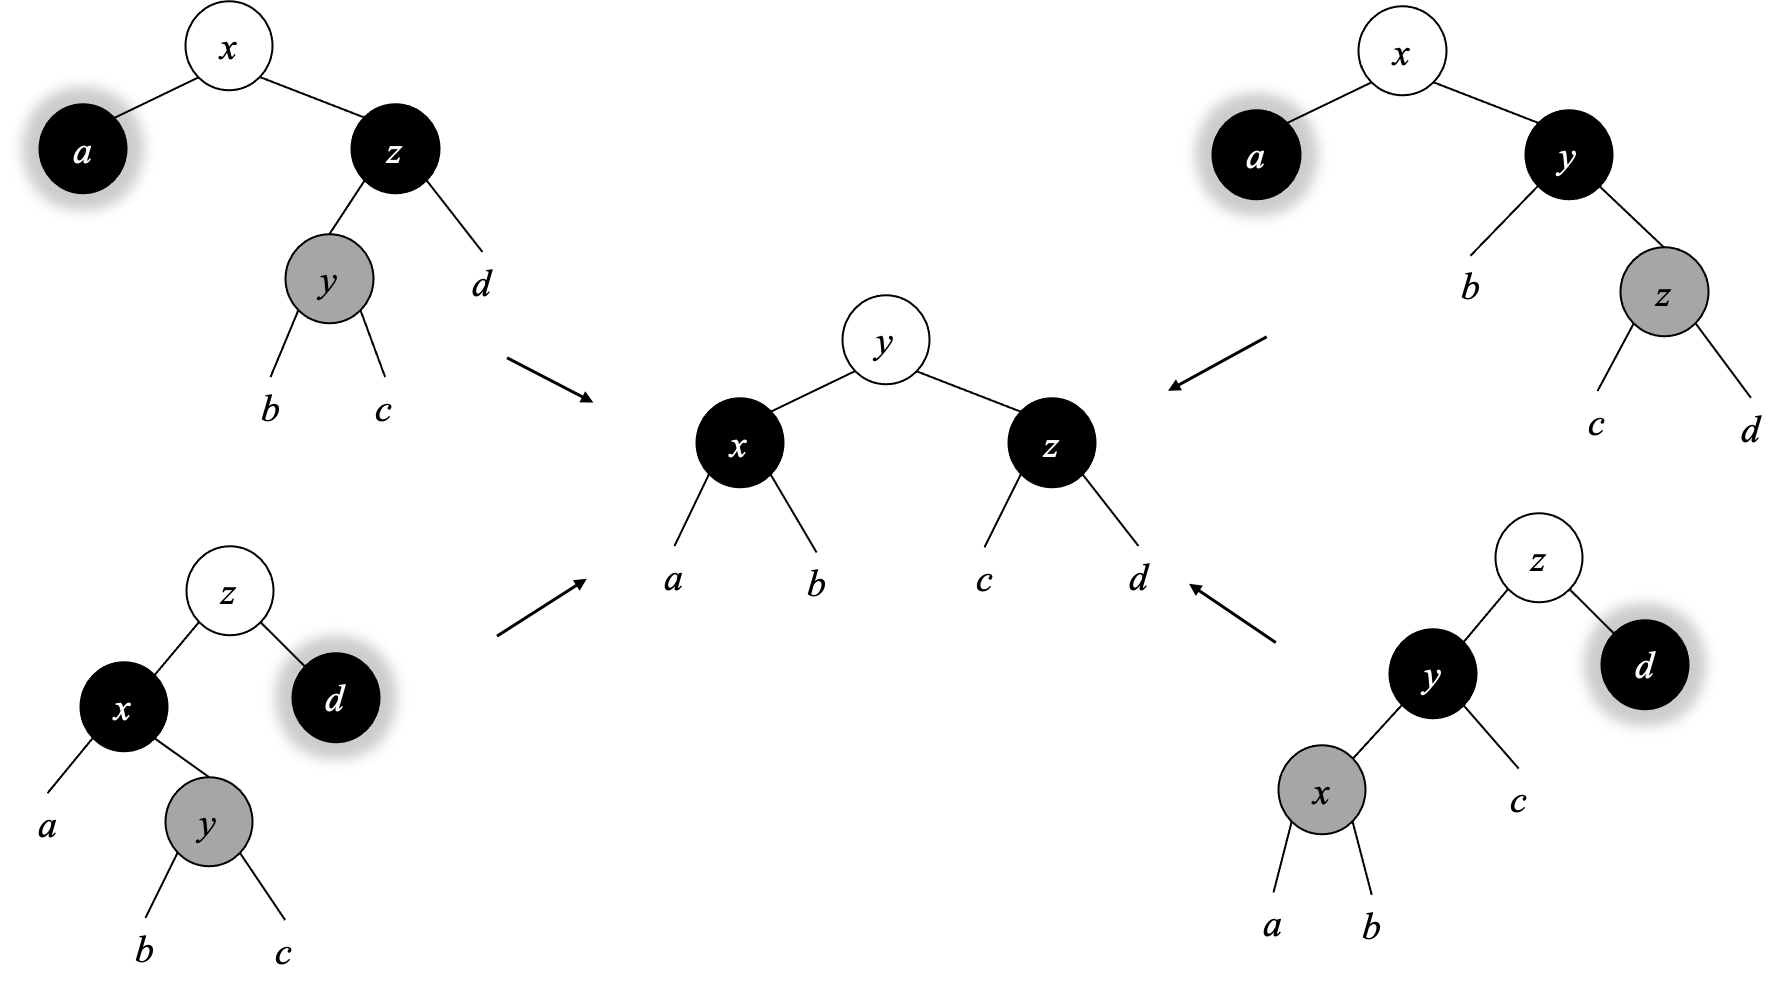
\includegraphics[scale=0.4]{img/del-case1}
   \caption{4种子情况可以修复为统一的形式}
   \label{fig:del-case1}
\end{figure}

我们通过模式匹配来处理这四种子情况:

\be
\resizebox{\textwidth}{!}{\ensuremath{
\begin{array}{rcl}
%\text{case 1 up left:} & & \\
fixB^2\ \mathcal{C}\ a_{\mathcal{B}^2}\ x\ (\mathcal{B}, (\mathcal{R}, b, y, c), z, d) & = & (\mathcal{C}, (\mathcal{B}, shiftB(a), x, b), y, (\mathcal{B}, c, z, d)) \\
%\text{case 1 up right:} & & \\
fixB^2\ \mathcal{C}\ a_{\mathcal{B}^2}\ x\ (\mathcal{B}, b, y, (\mathcal{R}, c, z, d)) & = & (\mathcal{C}, (\mathcal{B}, shiftB(a), x, b), y, (\mathcal{B}, c, z, d)) \\
%\text{case 1 bottom left:} & & \\
fixB^2\ \mathcal{C}\ (\mathcal{B}, a, x, (\mathcal{R}, b, y, c))\ z\ d_{\mathcal{B}^2} & = & (\mathcal{C}, (\mathcal{B}, a, x, b), y, (\mathcal{B}, c, z, shiftB(d))) \\
%\text{case 1 bottom right:} & & \\
fixB^2\ \mathcal{C}\ (\mathcal{B}, (\mathcal{R}, a, x, b), y, c)\ z\ d_{\mathcal{B}^2} & = & (\mathcal{C}, (\mathcal{B}, a, x, b), y, (\mathcal{B}, c, z, shiftB(d))) \\
\end{array}
}}
\label{eq:db-case-1}
\ee

其中$a_{\mathcal{B}^2}$表示节点$a$是双重黑色,可以是分枝节点或$\pmb{\varnothing}$。

\textbf{情况2:双重黑色节点的兄弟节点为红色。}可以通过旋转,将其变换为情况1或3。如图\ref{fig:del-case2}所示。

\begin{figure}[htbp]
  \centering
  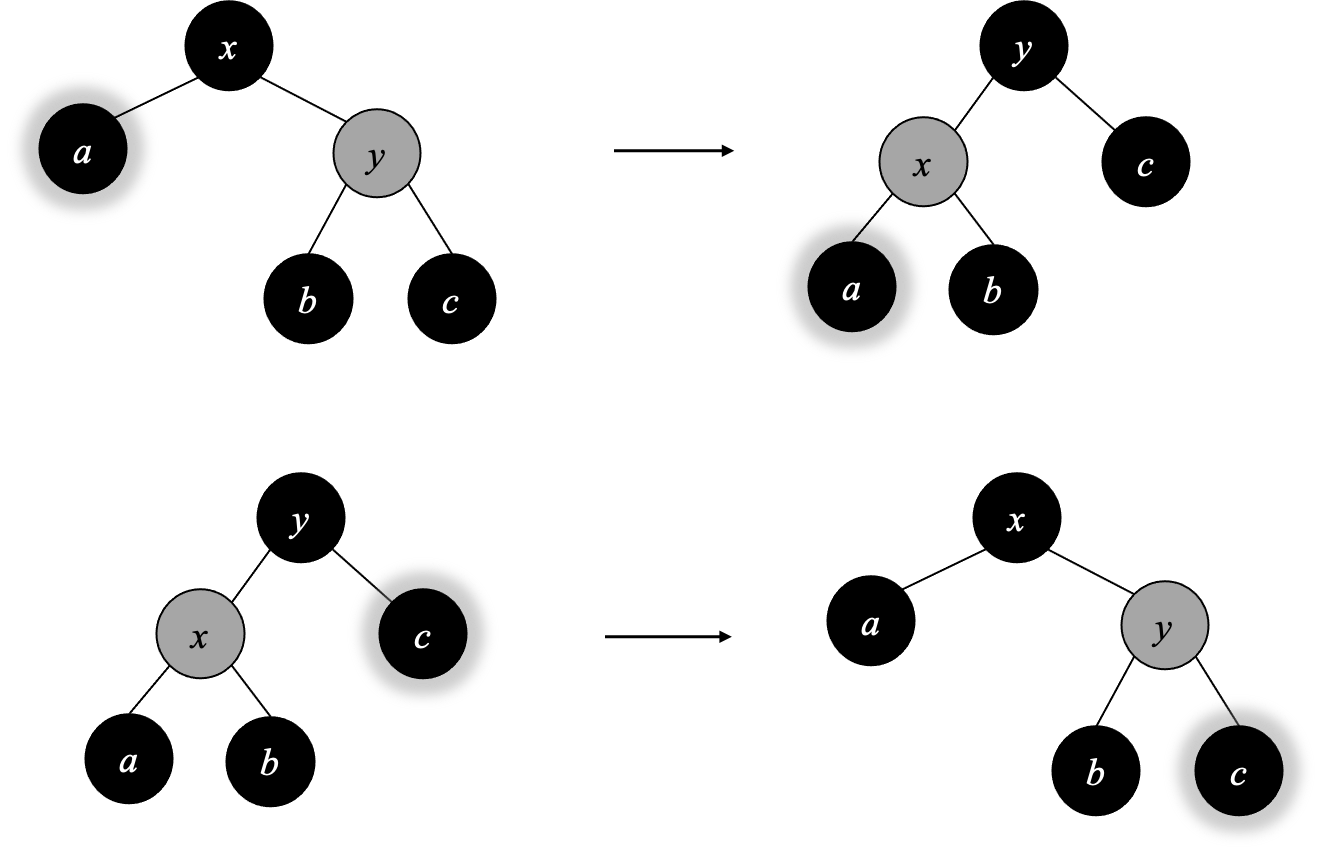
\includegraphics[scale=0.4]{img/del-case2}
  \caption{双重黑色节点的兄弟节点为红色}
  \label{fig:del-case2}
\end{figure}

我们在公式(\ref{eq:db-case-1})的基础上增加情况2的修复:

\be
%\resizebox{\textwidth}{!}{\ensuremath{
\begin{array}{rcl}
\text{...} & & \\
%\text{case 2 up:} & & \\
fixB^2\ \mathcal{B}\ a_{\mathcal{B}^2}\ x\ (\mathcal{R}, b, y, c) & = & fixB^2\ \mathcal{B}\ (fixB^2\ \mathcal{R}\ a\ x\ b)\ y\ c \\
%\text{case 2 bottom:} & & \\
fixB^2\ \mathcal{B}\ (\mathcal{R}, a, x, b)\ y\ c_{\mathcal{B}^2} & = & fixB^2\ \mathcal{B}\ a\ x\ (fixB^2\ \mathcal{R}\ b\ y\ c)
\end{array}
%}}
\label{eq:db-case-2}
\ee

\textbf{情况3:双重黑色的兄弟节点,该兄弟节点的两个子节点都是黑色。}这种情况下,我们将兄弟节点染成红色,将双重黑色变回黑色,然后将双重黑色属性向上传递一层到父节点。如图\ref{fig:del-case3}所示。

\begin{figure}[htbp]
  \centering
  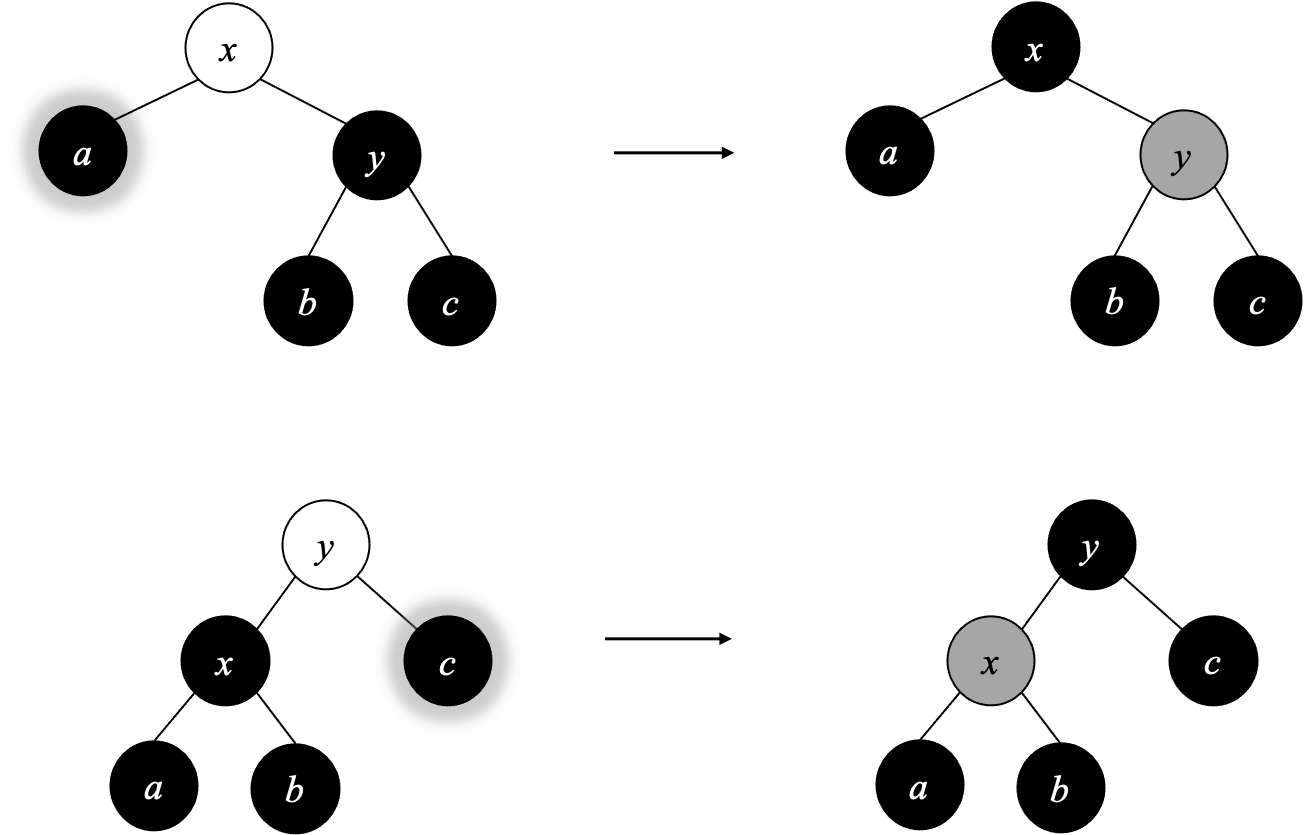
\includegraphics[scale=0.4]{img/del-case3}
  \caption{将双重黑色向上传递}
  \label{fig:del-case3}
\end{figure}

有两种对称情况:对于上方的情况,如果$x$是红色,则变为黑色,否则变为双重黑色;对于下方的情况,$y$的变化与此类似。我们继续在式(\ref{eq:db-case-2})的基础上增加此种修复:

\be
%\resizebox{\textwidth}{!}{\ensuremath{
\begin{array}{rcl}
\text{...} & & \\

fixB^2\ \mathcal{C}\ a_{\mathcal{B}^2}\ x\ (\mathcal{B}, b, y, c) & = & shiftB\ (\mathcal{C}, (shiftB\ a), x, (\mathcal{R}, b, y, c)) \\

fixB^2\ \mathcal{C}\ (\mathcal{B}, a, x, b)\ y\ c_{\mathcal{B}^2} & = & fixB^2\ \mathcal{B}\ a\ x\ (fixB^2\ \mathcal{R}\ b\ y\ c) \\

fixB^2\ \mathcal{C}\ l\ k\ r\ & = & (\mathcal{C}, l, k, r) \\
\end{array}
%}}
\label{eq:db-case-3}
\ee

如果没有匹配到上述三种模式,最后一行保持节点不变。双重黑色的修复是递归的。它中止于两种情况:一个是\textbf{情况1},双重黑色节点被消除了;另外一个是双重黑色向上移动,直到根节点,并最终恢复为黑色。下面的例子程序将以上情况汇总到一起:

\begin{Haskell}
-- the sibling is black, and has a red sub-tree
fixDB color a@(Node BB _ _ _) x (Node B (Node R b y c) z d)
      = Node color (Node B (shiftBlack a) x b) y (Node B c z d)
fixDB color BBEmpty x (Node B (Node R b y c) z d)
      = Node color (Node B Empty x b) y (Node B c z d)
fixDB color a@(Node BB _ _ _) x (Node B b y (Node R c z d))
      = Node color (Node B (shiftBlack a) x b) y (Node B c z d)
fixDB color BBEmpty x (Node B b y (Node R c z d))
      = Node color (Node B Empty x b) y (Node B c z d)
fixDB color (Node B a x (Node R b y c)) z d@(Node BB _ _ _)
      = Node color (Node B a x b) y (Node B c z (shiftBlack d))
fixDB color (Node B a x (Node R b y c)) z BBEmpty
      = Node color (Node B a x b) y (Node B c z Empty)
fixDB color (Node B (Node R a x b) y c) z d@(Node BB _ _ _)
      = Node color (Node B a x b) y (Node B c z (shiftBlack d))
fixDB color (Node B (Node R a x b) y c) z BBEmpty
      = Node color (Node B a x b) y (Node B c z Empty)
-- the sibling is red
fixDB B a@(Node BB _ _ _) x (Node R b y c)
      = fixDB B (fixDB R a x b) y c
fixDB B a@BBEmpty x (Node R b y c)
      = fixDB B (fixDB R a x b) y c
fixDB B (Node R a x b) y c@(Node BB _ _ _)
      = fixDB B a x (fixDB R b y c)
fixDB B (Node R a x b) y c@BBEmpty
      = fixDB B a x (fixDB R b y c)
-- the sibling and its 2 children are all black, move the blackness up
fixDB color a@(Node BB _ _ _) x (Node B b y c)
      = shiftBlack (Node color (shiftBlack a) x (Node R b y c))
fixDB color BBEmpty x (Node B b y c)
      = shiftBlack (Node color Empty x (Node R b y c))
fixDB color (Node B a x b) y c@(Node BB _ _ _)
      = shiftBlack (Node color (Node R a x b) y (shiftBlack c))
fixDB color (Node B a x b) y BBEmpty
      = shiftBlack (Node color (Node R a x b) y Empty)
-- otherwise
fixDB color l k r = Node color l k r
\end{Haskell}

删除算法的复杂度为$O(h)$,其中$h$为树的高度。由于红黑树保持平衡性,对于$n$个节点的树,$h = O(\lg n)$。

\begin{Exercise}
\Question{实现“标记——重建”删除算法:标记被删除的节点,但不进行真正的移除。当被标记的节点数目超过50\%时重建树。}
\end{Exercise}

\section{命令式红黑树算法$\star$}
\index{红黑树!命令式插入}

通过模式匹配和递归,我们简化了红黑树的实现。为了完整,我们给出命令式的实现。插入算法的第一步和二叉搜索树相同,接下来通过旋转操作修复平衡。

\begin{algorithmic}[1]
\Function{Insert}{$T, k$}
  \State $root \gets T$
  \State $x \gets$ \Call{Create-Leaf}{$k$}
  \State \Call{Color}{$x$} $\gets$ RED
  \State $p \gets$ NIL
  \While{$T \neq$ NIL}
    \State $p \gets T$
    \If{$k <$ \Call{Key}{$T$}}
      \State $T \gets $ \Call{Left}{$T$}
    \Else
      \State $T \gets $ \Call{Right}{$T$}
    \EndIf
  \EndWhile
  \State \Call{Parent}{$x$} $\gets p$
  \If{$p =$ NIL} \Comment{树$T$为空}
    \State \Return $x$
  \ElsIf{$k <$ \Call{Key}{$p$}}
    \State \Call{Left}{$p$} $\gets x$
  \Else
    \State \Call{Right}{$p$} $\gets x$
  \EndIf
  \State \Return \Call{Insert-Fix}{$root, x$}
\EndFunction
\end{algorithmic}

新节点为红色,接下来修复平衡。共有3种基本情况,每种都有左右对称的情况,总计6种情况。其中有两种可以合并,它们都有红色的“叔父”节点,我们可将父节点和叔父节点都变为黑色,将祖父节点变为红色:

\begin{algorithmic}[1]
\Function{Insert-Fix}{$T, x$}
  \While{\Call{Parent}{$x$} $\neq$ NIL and \textproc{Color}(\Call{Parent}{$x$}) = RED}
    \If{\textproc{Color}(\Call{Uncle}{$x$}) $=$ RED}
      \Comment{情况1:$x$的叔父节点是红色}
      \State \textproc{Color}(\Call{Parent}{$x$}) $\gets$ BLACK
      \State \textproc{Color}(\Call{Grand-Parent}{$x$}) $\gets$ RED
      \State \textproc{Color}(\Call{Uncle}{$x$}) $\gets$ BLACK
      \State $x \gets$ \Call{Grand-Parent}{$x$}
    \Else
      \Comment{$x$的叔父节点是黑色}
      \If{\Call{Parent}{$x$} = \textproc{Left}(\Call{Grand-Parent}{$x$})}
        \If{ $x =$ \textproc{Right}(\Call{Parent}{$x$})}
          \Comment{情况2:$x$是右子树}
          \State $x \gets$ \Call{Parent}{$x$}
          \State $T \gets$ \Call{Left-Rotate}{$T, x$}
        \EndIf
        \Comment{情况3:$x$是左子树}
        \State \textproc{Color}(\Call{Parent}{$x$}) $\gets$ BLACK
        \State \textproc{Color}(\Call{Grand-Parent}{$x$}) $\gets$ RED
        \State $T \gets$ \textproc{Right-Rotate}($T$, \Call{Grand-Parent}{$x$})
      \Else
         \If{ $x =$ \textproc{Left}(\Call{Parent}{$x$})}
          \Comment{情况2的对称}
          \State $x \gets$ \Call{Parent}{$x$}
          \State $T \gets$ \Call{Right-Rotate}{$T, x$}
        \EndIf
        \Comment{情况3的对称}
        \State \textproc{Color}(\Call{Parent}{$x$}) $\gets$ BLACK
        \State \textproc{Color}(\Call{Grand-Parent}{$x$}) $\gets$ RED
        \State $T \gets$ \textproc{Left-Rotate}($T$, \Call{Grand-Parent}{$x$})
      \EndIf
    \EndIf
  \EndWhile
  \State \Call{Color}{$T$} $\gets$ BLACK
  \State \Return $T$
\EndFunction
\end{algorithmic}

插入算法的复杂度为$O(\lg n)$,其中$n$是节点数。和$balance$函数对比,它们的处理逻辑并不相同。即使输入相同序列,也会构造出不同的红黑树。图\ref{fig:imperative-insert}给出了两棵红黑树,它们是使用和图\ref{fig:insert-example}中完全相同的序列构造出的。我们可以发现它们的不同。使用模式匹配的函数式算法存在一些性能损失。Okasaki在\cite{okasaki}中给出了详细分析。

\begin{figure}[htbp]
   \centering
   \includegraphics[scale=0.4]{img/clrs-fig-13-4}
   \includegraphics[scale=0.4]{img/python-insert}
   \caption{命令式算法构建出的红黑树}
   \label{fig:imperative-insert}
\end{figure}

红黑树的命令式删除算法更为复杂,参见本书附录A。

\section{小结}
红黑树是广泛使用的一种平衡二叉搜索树。我们在下一章介绍另外一种自平衡二叉树——AVL树。红黑树可以看作是其它复杂的数据结构的基础:将子节点的数目扩展到$k$个,并且保持树的平衡,就可以演化到B树。如果将数据存储在边上,而非节点中,就演化出基数树。在红黑树的实现中,为了修复平衡性,需要处理多种情况。Okasaki给出了一种简化方法,并激发了多种类似的实现\cite{rosetta}。本书中的AVL树、Splay树都是基于模式匹配方法实现的。

\section{附录:例子程序}

带有父节点引用的红黑树定义,默认节点为红色。

\begin{lstlisting}[language = Bourbaki]
data Node<T> {
    T key
    Color color
    Node<T> left
    Node<T> right
    Node<T> parent

    Node(T x) = Node(null, x, null, Color.RED)

    Node(Node<T> l, T k, Node<T> r, Color c) {
        left = l, key = k, right = r, color = c
        if left != null then left.parent = this
        if right != null then right.parent = this
    }

    Self setLeft(l) {
        left = l
        if l != null then l.parent = this
    }

    Self setRight(r) {
        right = r
        if r != null then r.parent = this
    }

    Node<T> sibling() = if parent.left == this then parent.right
                        else parent.left

    Node<T> uncle() = parent.sibling()

    Node<T> grandparent() = parent.parent
}
\end{lstlisting}

红黑树的插入:

\begin{lstlisting}[language = Bourbaki]
Node<T> insert(Node<T> t, T key) {
    root = t
    x = Node(key)
    parent = null
    while (t != null) {
        parent = t
        t = if (key < t.key) then t.left else t.right
    }
    if (parent == null) {    //tree is empty
        root = x
    } else if (key < parent.key) {
        parent.setLeft(x)
    } else {
        parent.setRight(x)
    }
    return insertFix(root, x)
}
\end{lstlisting}

插入后的平衡修复:

\begin{lstlisting}[language = Bourbaki]
// Fix the red->red violation
Node<T> insertFix(Node<T> t, Node<T> x) {
    while (x.parent != null and x.parent.color == Color.RED) {
        if (x.uncle().color == Color.RED) {
            // case 1: ((a:R x:R b) y:B c:R) ==> ((a:R x:B b) y:R c:B)
            x.parent.color = Color.BLACK
            x.grandparent().color = Color.RED
            x.uncle().color = Color.BLACK
            x = x.grandparent()
        } else {
            if (x.parent == x.grandparent().left) {
                if (x == x.parent.right) {
                    // case 2: ((a x:R b:R) y:B c) ==> case 3
                    x = x.parent
                    t = leftRotate(t, x)
                }
                // case 3: ((a:R x:R b) y:B c) ==> (a:R x:B (b y:R c))
                x.parent.color = Color.BLACK
                x.grandparent().color = Color.RED
                t = rightRotate(t, x.grandparent())
            } else {
                if (x == x.parent.left) {
                    // case 2': (a x:B (b:R y:R c)) ==> case 3'
                    x = x.parent
                    t = rightRotate(t, x)
                }
                // case 3': (a x:B (b y:R c:R)) ==> ((a x:R b) y:B c:R)
                x.parent.color = Color.BLACK
                x.grandparent().color = Color.RED
                t = leftRotate(t, x.grandparent())
            }
        }
    }
    t.color = Color.BLACK
    return t
}
\end{lstlisting}

\ifx\wholebook\relax \else
\begin{thebibliography}{99}

\bibitem{CLRS}
Thomas H. Cormen, Charles E. Leiserson, Ronald L. Rivest and Clifford Stein.
``Introduction to Algorithms, Second Edition''. ISBN:0262032937. The MIT Press. 2001 (《算法导论》中文版)

\bibitem{okasaki}
Chris Okasaki. ``FUNCTIONAL PEARLS Red-Black Trees in a Functional Setting''. J. Functional Programming. 1998

\bibitem{okasaki-blog}
Chris Okasaki. ``Ten Years of Purely Functional Data Structures''. \url{http://okasaki.blogspot.com/2008/02/ten-years-of-purely-functional-data.html}

\bibitem{wiki-rbt}
Wikipedia. ``Red-black tree''. \url{https://en.wikipedia.org/wiki/Red-black_tree}

\bibitem{lyn}
Lyn Turbak. ``Red-Black Trees''. \url{http://cs.wellesley.edu/~cs231/fall01/red-black.pdf} Nov. 2, 2001.

\bibitem{sgi-stl}
SGI STL. \url{http://www.sgi.com/tech/stl/}

\bibitem{rosetta}
Pattern matching. \url{http://rosettacode.org/wiki/Pattern_matching}

\end{thebibliography}

\expandafter\enddocument

\fi


\ifx\wholebook\relax \else

\documentclass[b5paper]{ctexart}
\usepackage[nomarginpar
  %, margin=.5in
]{geometry}

\addtolength{\oddsidemargin}{-0.05in}
\addtolength{\evensidemargin}{-0.05in}
\addtolength{\textwidth}{0.1in}

\usepackage[cn]{../../../prelude}

\setcounter{page}{1}

\begin{document}

\title{AVL树}

\author{刘新宇
\thanks{{\bfseries 刘新宇} \newline
  Email: liuxinyu95@gmail.com \newline}
  }

\maketitle
\fi

\markboth{AVL树}{基本算法}

\ifx\wholebook\relax
\chapter{AVL树}
\numberwithin{Exercise}{chapter}
\fi

\label{introduction} \index{AVL树}

为了解决平衡问题,红黑树限制在某一路径上的节点数。AVL树采用了更为直接方法:度量分枝间的差异。对于树$T$,定义:

\be
  \delta(T) = |r| - |l|
\ee

其中$|T|$表示树$T$的高度,$l$、$r$为左右子树。定义空树$\delta(\nil) = 0$。如果每棵子树$T$都有$\delta(T) = 0$,则树是完全平衡的。例如,一棵高度为$h$的完全二叉树有$n = 2^h - 1$个节点。除了叶子节点外,所有节点都不为空。$\delta(T)$的绝对值越小,树越平衡。我们称$\delta(T)$为二叉树的“平衡因子”。

\section{定义}
\index{AVL树!定义}

\begin{figure}[htbp]
   \centering
   \includegraphics[scale=0.5]{img/avl-example}
   \caption{AVL树} \label{fig:avl-example}
\end{figure}

一棵二叉搜索树称为AVL树,如果所有子树$T$都满足如下条件:

\be
  |\delta(T)| \leq 1
  \label{eq:avl-rule}
\ee

平衡因子$\delta(T)$只能是$\pm 1$、0。图\ref{fig:avl-example}给出了一棵AVL树的例子。如果树中有$n$个节点,这一定义保证了树的高度$h = O(\lg n)$。我们可以证明这个结论。一棵高为$h$的AVL树,其节点数目并不是一个固定的值。当它是完全二叉树时,含有的节点数目最多,为$2^h - 1$。我们关心它至少包含多少节点。定义$N(h)$代表高度为$h$的AVL树的最小节点数目。我们有:

\begin{itemize}
\item 空树$\nil$:$h = 0$,$N(0) = 0$;
\item 只有一个节点的树:$h = 1$,$N(1) = 1$;
\end{itemize}

图\ref{fig:N-h-relation}中给出了一个高度为$h$的AVL树$T$。它包含三部分:元素$k$和左右子树$l$、$r$。树的高度$h$和子树高度之间满足下面的关系:

\begin{figure}[htbp]
   \centering
   \includegraphics[scale=0.5]{img/Nh-lvr}
   \caption{高度为$h$的AVL树,其中一棵子树高$h - 1$,另外一棵的高度不小于$h - 2$}
   \label{fig:N-h-relation}
\end{figure}

\be
  h = \max(|l|, |r|) + 1
\ee

因此必然存在一个子树的高度为$h - 1$。根据AVL树的定义,有 $||l| -|r|| \leq 1$。所以另外一棵子树的高度不会小于$h - 2$。而$T$所包含的节点数为两个子树的节点数和加1(节点$T$本身):

\be
  N(h) = N(h-1) + N(h-2) + 1
  \label{eq:Fibonacci-like}
\ee

这一递归形式让我们联想起斐波那契数列。如果定义$N'(h) = N(h) + 1$,我们就可以将(\ref{eq:Fibonacci-like})转换成斐波那契数列的递归关系:

\be
  N'(h) = N'(h-1) + N'(h-2)
\ee

\begin{lemma}
\label{lemma:N-phi}
若$N(h)$表示高为$h$的AVL树的节点数目最小值,令$N'(h) = N(h) + 1$,则:

\be
  N'(h) \geq \phi^h
\ee

其中$\phi = \dfrac{\sqrt{5}+1}{2}$,称为黄金分割比。
\end{lemma}

\begin{proof}[证明]
使用数学归纳法。当$h = 0$或1时:
\begin{itemize}
\item $h = 0$, $N'(0) = 1 \geq \phi^0 = 1$
\item $h = 1$, $N'(1) = 2 \geq \phi^1 = 1.618...$
\end{itemize}

对于递推情况,设$N'(h) \geq \phi^h$。
\[
  \begin{array}{lll}
  N'(h+1) & = N'(h) + N'(h-1) & \{\text{斐波那契}\} \\
          & \geq \phi^h + \phi^{h-1} & \{\text{递推假设}\}\\
          & = \phi^{h-1}(\phi + 1) & \{\phi + 1 = \phi^2 = \dfrac{\sqrt{5}+3}{2}\} \\
          & = \phi^{h+1}
 \end{array}
\]
\end{proof}

由引理\ref{lemma:N-phi},我们立即得到下面的结果:

\be
  h \leq log_{\phi}(n+1) = log_{\phi}2 \cdot \lg (n+1) \approx 1.44 \lg (n+1)
  \label{eq:AVL-height}
\ee

这一不等式说明AVL树的高度为$O(\lg n)$,从而保证了平衡性。插入和删除会改变树的结构,导致平衡因子的绝对值超出1,需要通过修复使得$|\delta| < 1$。传统的修复方法是树旋转。我们给出一种基于模式匹配的方法简化实现。思路类似于函数式的红黑树\cite{okasaki}。由于这种“改变——恢复”的策略,AVL树也是一种自平衡二叉树。我们复用二叉搜索树的定义,尽管平衡因子$\delta$可以递归地求出,为了方便,我们在每个非空节点$T = (l, k, r, \delta)$中保存平衡因子的值,并在改变树结构时更新它\footnote{也可以保存树的高度而非$\delta$\cite{py-avl}。}。下面的例子程序增加了一个整型变量$\delta$:

\lstset{frame = single}
\begin{Haskell}
data AVLTree a = Empty | Br (AVLTree a) a (AVLTree a) Int
\end{Haskell}

AVL树的$lookup$、$\max$、$\min$等操作和二叉搜索树相同,而插入和删除操作是特殊的。

\section{插入}
\index{AVL树!插入}

向AVL树中插入一个新元素时,平衡因子的绝对值$|\delta(T)|$可能超过1。我们用类似红黑树修复的模式匹配方法恢复平衡。插入元素$x$后,包含它的子树高度最多增加1。我们需要沿着插入路径递归地更新平衡因子。定义插入结果为一对值$(T', \Delta H)$,其中$T'$为插入后的树,$\Delta H$为高度的增加值。我们将二叉搜索树的插入算法修改如下:

\be
insert\ x = \textit{fst} \circ ins\ x
\ee

其中$\textit{fst}\ (a, b) = a$返回一对值中的第一个。$ins\ x\ T$将元素$x$插入到树$T$中:

\be
\begin{array}{rcl}
ins\ x\ \nil & = & ((\nil, x, \nil, 0), 1) \\
ins\ x\ (l, k, r, \delta) & = & \begin{cases}
  x < k: tree\ (ins\ x\ l)\ k\ (r, 0)\ \delta \\
  x > k: tree\ (l, 0)\ k\ (ins\ x\ r)\ \delta \\
\end{cases}
\end{array}
\label{eq:ins}
\ee

如果树为空$\nil$,结果为包含$x$的叶子节点,平衡因子为0,高度增加1。否则,令$T = (l, k, r, \delta)$。我们比较$x$和$k$,如果$x < k$,我们递归地将$x$插入到左子树$l$中,否则插入右子树$r$。递归插入的结果也是一对值$(l', \Delta l)$或$(r', \Delta r)$。我们通过函数$tree$调整平衡因子并更新高度,它接受4个参数:$(l', \Delta l)$、$k$、$(r', \Delta r)$、$\delta$,并产生结果$(T', \Delta H)$。其中$T'$为新树,$\Delta H$定义如下:

\be
  \Delta H = |T'| - |T|
\ee

它可以进一步分解为4种情况:

\be
\begin{array}{rcl}
  \Delta H & = & |T'| - |T| \\
           & = & 1 + \max(|r'|, |l'|) - (1 + \max(|r|, |l|)) \\
           & = & \max(|r'|, |l'|) - \max(|r|, |l|) \\
           & = & \begin{cases}
\delta \geq 0, \delta' \geq 0: & \Delta r \\
\delta \leq 0, \delta' \geq 0: & \delta + \Delta r \\
\delta \geq 0, \delta' \leq 0: & \Delta l - \delta \\
\text{否则}: & \Delta l
\end{cases}
\end{array}
\ee

其中$\delta' = \delta(T') = |r'| - |l'|$,是变化后的平衡因子。附录B给出了相关证明。在平衡调整前,还需要确定新的平衡因子$\delta'$。

\be
\begin{array}{rcl}
\delta' & = & |r'| - |l'| \\
        & = & |r| + \Delta r - (|l| + \Delta l) \\
        & = & |r| - |l| + \Delta r - \Delta l \\
        & = & \delta + \Delta r - \Delta l \\
\end{array}
\ee

使用树的高度变化和平衡因子,就可进一步定义(\ref{eq:ins})中的函数$tree$:

\be
tree\ (l', \Delta l)\ k\ (r', \Delta r)\ \delta =
  balance\ (l', k, r', \delta')\ \Delta H
\ee

下面的例子程序实现了目前给出的结论:

\begin{Haskell}
insert x  = fst . ins x where
    ins x Empty = (Br Empty x Empty 0, 1)
    ins x (Br l k r d)
        | x < k = tree (ins x l) k (r, 0) d
        | x > k = tree (l, 0) k (ins x r) d

tree (l, dl) k (r, dr) d = balance (Br l k r d') deltaH where
    d' = d + dr - dl
    deltaH | d >=0 && d' >=0 = dr
           | d <=0 && d' >=0 = d+dr
           | d >=0 && d' <=0 = dl - d
           | otherwise = dl
\end{Haskell}

\subsection{平衡调整}
\index{AVL树!平衡调整}
共有4种情况需要修复,如图\ref{fig:avl-insert-fix}所示。平衡因子为$\pm 2$超出了$[-1, 1]$范围。我们将其统一调整为图中心的结构,使得$\delta(y) = 0$。

\begin{figure}[htbp]
  \centering
  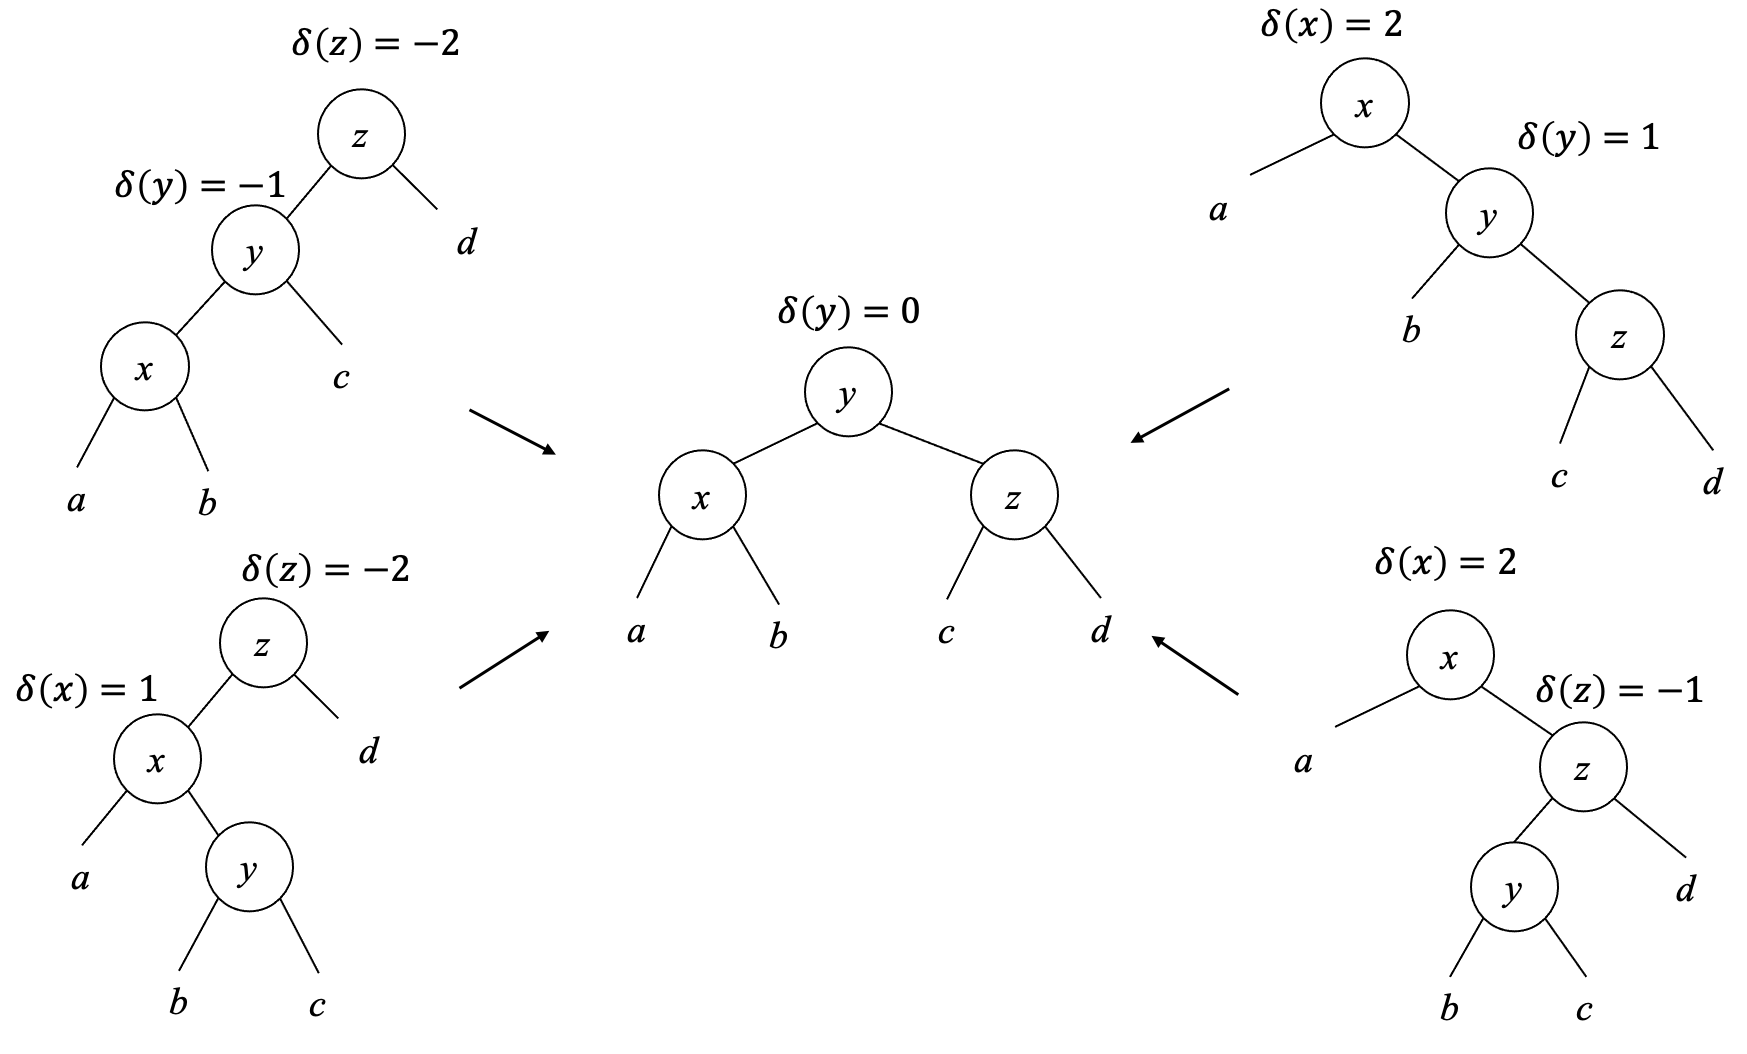
\includegraphics[scale=0.4]{img/avl-insert-fix}
  \caption{将4种情况修复为统一形式}
  \label{fig:avl-insert-fix}
\end{figure}

我们称这4种情况为左-左、右-右、右-左、左-右。记调整前的平衡因子为$\delta(x)$、$\delta(y)$、$\delta(z)$;调整后的平衡因子为$\delta'(x)$、$\delta'(y) = 0$、$\delta'(z)$。它们的关系如下。附录B给出了证明。

\begin{center}
左-左 \quad \quad \quad 右-右
\end{center}

\be
\begin{array}{cc}
  \begin{cases}
    \delta'(x) & = \delta(x) \\
    \delta'(y) & = 0 \\
    \delta'(z) & = 0 \\
  \end{cases}
&
  \begin{cases}
    \delta'(x) & = 0 \\
    \delta'(y) & = 0 \\
    \delta'(z) & = \delta(z) \\
  \end{cases}
\end{array}
\label{eq:rr-result}
\ee

右-左和左-右相同:

\be
  \begin{array}{l}
  \delta'(x) = \begin{cases}
    \delta(y) = 1: & -1 \\
    \text{否则}: & 0 \\
    \end{cases} \\
  \delta'(y) = 0 \\
  \delta'(z) = \begin{cases}
    \delta(y) = -1: & 1 \\
    \text{否则}: & 0 \\
    \end{cases} \\
  \end{array}
  \label{eq:rl-result}
\ee

利用模式匹配,定义修复为:

\be
\resizebox{\textwidth}{!}{\ensuremath{
\begin{array}{rcl}
balance\ (((a, x, b, \delta(x)), y, c, -1), z, d, -2)\ \Delta H & = & ((a, x, b, \delta(x)), y, (c, z, d, 0), 0, \Delta H -1) \\
balance\ (a, x, (b, y, (c, z, d, \delta(z)), 1), 2)\ \Delta H & = & ((a, x, b, 0), y, (c, z, d, \delta(z)), 0, \Delta H -1) \\
balance\ ((a, x, (b, y, c, \delta(y)), 1), z, d, -2)\ \Delta H & = & ((a, x, b, \delta'(x)), y, (c, z, d, \delta'(z)), 0, \Delta H - 1) \\
balance\ (a, x, ((b, y, c, \delta(y)), z, d, -1), 2)\ \Delta H & = & ((a, x, b, \delta'(x)), y, (c, z, d, \delta'(z)), 0, \Delta H - 1) \\
balance\ T\ \Delta H & = & (T, \Delta H) \\
\end{array}
}}
\ee

其中$\delta'(x)$和$\delta'(z)$按照式(\ref{eq:rl-result})定义。如果没有匹配任何模式,则保持树不变。下面是相应的例子程序:

\begin{Haskell}
balance (Br (Br (Br a x b dx) y c (-1)) z d (-2)) dH =
            (Br (Br a x b dx) y (Br c z d 0) 0, dH-1)
balance (Br a x (Br b y (Br c z d dz)    1)    2) dH =
            (Br (Br a x b 0) y (Br c z d dz) 0, dH-1)
balance (Br (Br a x (Br b y c dy)    1) z d (-2)) dH =
            (Br (Br a x b dx') y (Br c z d dz') 0, dH-1) where
    dx' = if dy ==  1 then -1 else 0
    dz' = if dy == -1 then  1 else 0
balance (Br a x (Br (Br b y c dy) z d (-1))    2) dH =
            (Br (Br a x b dx') y (Br c z d dz') 0, dH-1) where
    dx' = if dy ==  1 then -1 else 0
    dz' = if dy == -1 then  1 else 0
balance t d = (t, d)
\end{Haskell}

插入算法的复杂度和树的高度成正比,根据式(\ref{eq:AVL-height}),对于$n$个节点的树,$insert$的复杂度为$O(\lg n)$。

\subsection{检验}
\index{AVL树!检验}

判断一棵树是否是AVL树需要检查两点:(1)是否是二叉搜索树;(2)对于每棵子树$T$,式(\ref{eq:avl-rule}):$\delta(T) \leq 1$是否成立。下面的函数递归地检查子树间的高度差:

\be
\begin{array}{rcl}
avl?\ \nil & = & \textit{True} \\
avl?\ T & = & avl?\ l\ \text{且}\ avl?\ r\ \text{且}\ ||r| - |l|| \leq 1 \\
\end{array}
\ee

其中$l$、$r$分别是左右子树,高度递归计算如下:

\be
\begin{array}{rcl}
|\nil| & = & 0 \\
|T| & = & 1 + \max(|r|, |l|) \\
\end{array}
\ee

下面的例子程序实现了AVL树的高度检查:
\begin{Haskell}
isAVL Empty = True
isAVL (Br l _ r _) = isAVL l && isAVL r && abs (height r - height l) <= 1

height Empty = 0
height (Br l _ r _) = 1 + max (height l) (height r)
\end{Haskell}

\begin{Exercise}
\Question{我们只验证了AVL树的高度性质,完成验证程序检查一棵二叉树是否是AVL树。}
\end{Exercise}

\section{命令式算法$\bigstar$}
\index{AVL树!命令式插入}

为了完整,本节给出AVL树的命令式算法。和红黑树的命令式算法相似,我们先按二叉搜索树将新元素插入,然后再通过旋转操作恢复平衡。

\begin{algorithmic}[1]
\Function{Insert}{$T, k$}
  \State $root \gets T$
  \State $x \gets$ \Call{Create-Leaf}{$k$}
  \State \Call{$\delta$}{$x$} $\gets 0$
  \State $parent \gets$ NIL
  \While{$T \neq$ NIL}
    \State $parent \gets T$
    \If{$k <$ \Call{Key}{$T$}}
      \State $T \gets $ \Call{Left}{$T$}
    \Else
      \State $T \gets $ \Call{Right}{$T$}
    \EndIf
  \EndWhile
  \State \Call{Parent}{$x$} $\gets parent$
  \If{$parent =$ NIL} \Comment{树$T$为空}
    \State \Return $x$
  \ElsIf{$k <$ \Call{Key}{$parent$}}
    \State \Call{Left}{$parent$} $\gets x$
  \Else
    \State \Call{Right}{$parent$} $\gets x$
  \EndIf
  \State \Return \Call{AVL-Insert-Fix}{$root, x$}
\EndFunction
\end{algorithmic}

插入新元素后,树的高度可能增加,因此平衡因子$\delta$也会变化。插入到右侧可能使$\delta$增加1,插入左侧可能使$\delta$减少1。我们从$x$开始,自底向上修复平衡,直到根节点。记新的平衡因子为$\delta'$,共有3种情况:

\begin{itemize}
\item $|\delta| = 1$、$|\delta'| = 0$。插入后树处于平衡状态。父节点的高度没有变化。

\item $|\delta| = 0$、$|\delta'| = 1$。左右子树之一的高度增加了,需要继续向上检查平衡。

\item $|\delta| = 1$、$|\delta'| = 2$。需要旋转以修复平衡。
\end{itemize}

\begin{algorithmic}[1]
\Function{AVL-Insert-Fix}{$T, x$}
  \While{\Call{Parent}{$x$} $\neq$ NIL}
    \State $\delta \gets $ \textproc{$\delta$}(\Call{Parent}{$x$})
    \If{$x = $ \textproc{Left}(\Call{Parent}{$x$})}
      \State $\delta' \gets \delta - 1$
    \Else
      \State $\delta' \gets \delta + 1$
    \EndIf
    \State \textproc{$\delta$}(\Call{Parent}{$x$}) $\gets \delta'$
    \State $P \gets $ \Call{Parent}{$x$}
    \State $L \gets $ \Call{Left}{$x$}
    \State $R \gets $ \Call{Right}{$x$}
    \If{$|\delta| = 1$ and $|\delta'| = 0$} \Comment{高度没有变化}
      \State \Return $T$
    \ElsIf{$|\delta| = 0$ and $|\delta'| = 1$} \Comment{继续自底向上更新}
      \State $x \gets P$
    \ElsIf{$|\delta| = 1$ and $|\delta'| = 2$}
      \If{$\delta'=2$}
        \If{$\delta(R) = 1$} \Comment{右-右}
          \State $\delta(P) \gets 0$ \Comment{根据式(\ref{eq:rr-result})}
          \State $\delta(R) \gets 0$
          \State $T \gets $ \Call{Left-Rotate}{$T, P$}
        \EndIf
        \If{$\delta(R) = -1$} \Comment{右-左}
          \State $\delta_y \gets $ \textproc{$\delta$}(\Call{Left}{$R$}) \Comment{根据式(\ref{eq:rl-result})}
          \If{$\delta_y = 1$}
            \State $\delta(P) \gets -1$
          \Else
            \State $\delta(P) \gets 0$
          \EndIf
          \State \textproc{$\delta$}(\Call{Left}{$R$}) $\gets 0$
          \If{$\delta_y = -1$}
            \State $\delta(R) \gets 1$
          \Else
            \State $\delta(R) \gets 0$
          \EndIf
          \State $T \gets $ \Call{Right-Rotate}{$T, R$}
          \State $T \gets $ \Call{Left-Rotate}{$T, P$}
        \EndIf
      \EndIf
      \If{$\delta' = -2$}
        \If{$\delta(L) = -1$} \Comment{左-左}
          \State $\delta(P) \gets 0$
          \State $\delta(L) \gets 0$
          \State \Call{Right-Rotate}{$T, P$}
        \Else \Comment{左-右}
          \State $\delta_y \gets $ \textproc{$\delta$}(\Call{Right}{$L$})
          \If{$\delta_y = 1$}
            \State $\delta(L) \gets -1$
          \Else
            \State $\delta(L) \gets 0$
          \EndIf
          \State \textproc{$\delta$}(\Call{Right}{$L$}) $\gets 0$
          \If{$\delta_y = -1$}
            \State $\delta(P) \gets 1$
          \Else
            \State $\delta(P) \gets 0$
          \EndIf
          \State \Call{Left-Rotate}{$T, L$}
          \State \Call{Right-Rotate}{$T, P$}
        \EndIf
      \EndIf
      \State break
    \EndIf
  \EndWhile
  \State \Return $T$
\EndFunction
\end{algorithmic}

除了旋转,还需要更新平衡因子$\delta$。右-右和左-左情况需要进行一次旋转;而右-左和左-右需要进行两次旋转。我们略过了AVL树的删除算法,附录B给出了删除的实现。

AVL树是1962年由Adelson-Velskii和Landis\cite{wiki-avl}、\cite{TFATP}提出的,并以两位作者的名字命名。它比红黑树更早。AVL树和红黑树都是自平衡二叉树,大多数操作的复杂度都是$O(\lg n)$。式(\ref{eq:AVL-height})使得AVL树的平衡性更为严格。在大量查询的情况下,其表现要好于红黑树\cite{wiki-avl}。但红黑树在频繁插入和删除的情况下性能更佳。很多程序库使用红黑树作为自平衡二叉搜索树的内部实现,AVL树同样也可以直观、高效地解决平衡问题。

\section{附录:例子程序}

AVL树的定义:

\begin{lstlisting}[language = Bourbaki]
data Node<T> {
    int delta
    T key
    Node<T> left
    Node<T> right
    Node<T> parent
}
\end{lstlisting}

平衡修复:

\begin{lstlisting}[language = Bourbaki]
Node<T> insertFix(Node<T> t, Node<T> x) {
    while (x.parent != null ) {
        var (p, l, r) = (x.parent, x.parent.left, x.parent.right)
        var d1 = p.delta
        var d2 = if x == parent.left then d1 - 1 else d1 + 1
        p.delta = d2

        if abs(d1) == 1 and abs(d2) == 0 {
            return t
        } else if abs(d1) == 0 and abs(d2) == 1 {
            x = p
        } else if abs(d1) == 1 and abs(d2) == 2 {
            if d2 == 2 {
                if r.delta == 1 {    //Right-right
                    p.delta = 0
                    r.delta = 0
                    t = rotateLeft(t, p)
                } else if r.delta == -1 {    //Right-Left
                    var dy = r.left.delta
                    p.delta = if dy == 1 then -1 else 0
                    r.left.delta = 0
                    r.delta = if dy == -1 then 1 else 0
                    t = rotateRight(t, r)
                    t = rotateLeft(t, p)
                }
            } else if d2 == -2 {
                if l.delta == -1 {    //Left-left
                    p.delta = 0
                    l.delta = 0
                    t = rotateRight(t, p)
                } else if l.delta == 1 {    //Left-right
                    var dy = l.right.delta
                    l.delta = if dy == 1 then -1 else 0
                    l.right.delta = 0
                    p.delta = if dy == -1 then 1 else 0
                    t = rotateLeft(t, l)
                    t = rotateRight(t, p)
                }
            }
            break
        }
    }
    return t
}
\end{lstlisting}

\ifx\wholebook\relax \else
\section{参考答案}
\shipoutAnswer

\begin{thebibliography}{99}

\bibitem{hackage-avl}
Data.Tree.AVL \url{http://hackage.haskell.org/packages/archive/AvlTree/4.2/doc/html/Data-Tree-AVL.html}

\bibitem{okasaki}
Chris Okasaki. ``FUNCTIONAL PEARLS Red-Black Trees in a Functional Setting''. J. Functional Programming. 1998

\bibitem{wiki-avl}
Wikipedia. ``AVL tree''. \url{https://en.wikipedia.org/wiki/AVL_tree}

\bibitem{TFATP}
Guy Cousinear, Michel Mauny. ``The Functional Approach to Programming''. Cambridge University Press; English Ed edition (October 29, 1998). ISBN-13: 978-0521576819

\bibitem{py-avl}
Pavel Grafov. ``Implementation of an AVL tree in Python''. \url{http://github.com/pgrafov/python-avl-tree}
\end{thebibliography}

\end{document}
\fi


\ifx\wholebook\relax \else
% ------------------------

\documentclass[b5paper]{ctexart}
\usepackage[nomarginpar
  %, margin=.5in
]{geometry}

\addtolength{\oddsidemargin}{-0.05in}
\addtolength{\evensidemargin}{-0.05in}
\addtolength{\textwidth}{0.1in}

\usepackage[cn]{../../../prelude}

\setcounter{page}{1}

\begin{document}

\title{基数树}

\author{刘新宇
\thanks{{\bfseries 刘新宇 } \newline
  Email: liuxinyu95@gmail.com \newline}
  }

\maketitle
\fi

\markboth{基数树}{基本算法}

\ifx\wholebook\relax
\chapter{基数树}
\numberwithin{Exercise}{chapter}
\fi

%\section{简介}
\label{introduction} \index{基数树}

排序二叉树将信息存储在节点中。我们可以用边(edge)来携带信息么?基数树(Radix tree),包括trie、前缀树、后缀树就是根据这一思路设计出的数据结构。它们产生于1960年代,被广泛用于编译器\cite{okasaki-int-map}和生物信息处理(如DNA模式匹配)\cite{wiki-suffix-tree}等领域。

\begin{figure}[htbp]
  \centering
  \includegraphics[scale=0.4]{img/radix-tree.ps}
  \caption{基数树}
  \label{fig:radix-tree}
\end{figure}

图\ref{fig:radix-tree}展示了一棵基数树。它包含了二进制串1011、10、011、100、0。如果查找二进制数$k=(b_0b_1...b_n)_2$,我们首先检查左侧的最高位$b_0$。若为0,则转向左子树继续查找;若为1,则转向右子树。接着,我们检查第二位,并重复这一过程直到处理完所有的$n$位或到达某一叶子节点。我们并不需要在节点中存储键(key),这一信息由边来代表。图\ref{fig:radix-tree}标注在节点中的键仅仅是为了示意。对于整数类型的键,我们可以使用二进制,并利用位运算进行操作。

\section{整数trie}
\label{int-trie} \index{基数树!整数trie}

我们称图\ref{fig:radix-tree}所示的数据结构为\emph{binary trie}。Trie是Edward Fredkin在1960年提出的。它来自英文单词re\textbf{trie}val。Fredkin将其读作/'tri:/,但其他人读作/'trai/(和英文单词try的发音相同)\cite{wiki-trie}。有些情况下trie也被称为前缀树,在本章中,trie和前缀树分指不同的数据结构。一棵binary trie是一种特殊的二叉树,每个键的位置由它的二进制位来决定。0表示“向左”,1表示“向右”\cite{okasaki-int-map}。考虑图\ref{fig:big-endian-trie}中的trie,3个不同串``11''、``011''、``0011''代表同一个十进制整数3。

\begin{figure}[htbp]
  \centering
  \includegraphics[scale=0.4]{img/big-endian-trie.ps}
  \caption{大端(big-endian)trie}
  \label{fig:big-endian-trie}
\end{figure}

如果把前面的0也当作有效位,在一个32位整数的系统中,向空trie插入1,结果将是一棵32层的树。为了解决这一问题,Okasaki建议使用小端整数\cite{okasaki-int-map}。二进制数的最高位(MSB)通常在左边,最低位(LSB)在右边。这种形式称为大端整数,反之最高位在右边称为小端整数。使用小端,1表示为$(1)_2$,、2表示为$(01)_2$、3表示为$(11)_2$……

\subsection{定义}
我们可以重用二叉树的定义。一个节点要么为空,要么包含左右子树和一个值(值可以为空)左子树编码为0,右子树编码为1。

\lstset{frame = single}
\begin{Haskell}
data IntTrie a = Empty
               | Branch (IntTrie a) (Maybe a) (IntTrie a)
\end{Haskell}

对于binary trie中的任一节点,其对应的整数键是由节点的位置唯一确定的。因此我们无需在节点中存储键,而只需存储值。键的类型被固定为整数,如果值的类型为$A$,则树的类型为$IntTrie\ A$。

\subsection{插入}
\index{整数trie!插入}

当插入整数键$k$和值$v$时,我们将$k$转换成二进制。如果$k$是偶数,最低位是0,我们递归向左子树插入;如果$k$是奇数,最低位是1,我们递归向右子树插入。接下来我们将$k$除以2取整以去掉最低位。对于非空的trie树$T = (l, v', r)$,其中$l$、$r$是左右子树,$v'$是值(可为空),函数$insert$的定义如下:

\be
\begin{array}{rcl}
insert\ \nil\ k\ v & = & insert (\nil, \textit{Nothing}, \nil)\ k\ v \\
insert\ (l, v', r)\ 0\ v & = & (l, \textit{Just}\ v, r) \\
insert\ (l, v', r)\ k\ v & = & \begin{cases}
  even(k): & (insert\ l\ \dfrac{k}{2}\ v, v', r) \\
  odd(k) : & (l, v', insert\ r\ \lfloor \dfrac{k}{2} \rfloor\ v) \\
\end{cases}
\end{array}
\ee

如果$k = 0$,我们将$v$存入节点。如果$T = \nil$,结果为$(\nil, \textit{Just}\ v, \nil)$。只要$k \neq 0$,我们就根据$k$的奇偶性前进,遇到$\nil$就建立一个空叶子节点$(\nil, \textit{Nothing}, \nil)$。如果$k$已经存在,这一算法覆盖以前的值。我们也可以用一个列表存储多个值,并将$v$添加到列表中。图\ref{int-trie}的例子是依次插入映射对\{$ 1 \rightarrow a, 4 \rightarrow b, 5 \rightarrow c, 9 \rightarrow d$\}的结果。下面的例子程序实现了$insert$函数:

\begin{figure}[htbp]
  \centering
  \includegraphics[scale=0.5]{img/int-trie.ps}
  \caption{用小端整数trie,包含映射:
          \{$ 1 \rightarrow a, 4 \rightarrow b, 5 \rightarrow c, 9 \rightarrow d$\}}
  \label{fig:int-trie}
\end{figure}

\begin{Haskell}
insert Empty k x = insert (Branch Empty Nothing Empty) k x
insert (Branch l v r) 0 x = Branch l (Just x) r
insert (Branch l v r) k x | even k    = Branch (insert l (k `div` 2) x) v r
                          | otherwise = Branch l v (insert r (k `div` 2) x)
\end{Haskell}

也可以用命令式的方式定义插入算法。由于key是小端整数,插入时,我们需要从右侧逐位进行处理。若为0,则递归插入左子树;若为1,则插入右子树。如果子树为空,我们需要创建一个新节点。重复这一步骤直到处理完最后一位(最左侧的位)后停止。

%\begin{algorithm}
\begin{algorithmic}[1]
\Function{Insert}{$T, k, v$}
  \If{$T =$ NIL}
    \State $T \gets$ \Call{Empty-Node}{}
  \EndIf
  \State $p \gets T$
  \While{$k \neq 0$}
    \If{\Call{Even?}{$k$}}
      \If{\Call{Left}{$p$} = NIL}
        \State \Call{Left}{$p$} $\gets$ \Call{Empty-Node}{}
      \EndIf
      \State $p \gets$ \Call{Left}{$p$}
    \Else
      \If{\Call{Right}{$p$} = NIL}
        \State \Call{Right}{$p$} $\gets$ \Call{Empty-Node}{}
      \EndIf
      \State $p \gets$ \Call{Right}{$p$}
    \EndIf
    \State $k \gets \lfloor k/2 \rfloor$
  \EndWhile
  \State \Call{Data}{$p$} $\gets v$
  \State \Return $T$
\EndFunction
\end{algorithmic}
%\end{algorithm}

插入算法接受3个参数:一棵Trie树$T$、要插入的整数$k$和相应的数据$v$。下面的Python例子程序实现了这一算法。这段例子程序使用了位运算来判断奇偶和移位。

\lstset{language=Python}
\begin{lstlisting}
def insert(t, key, value = None):
    if t is None:
        t = IntTrie()
    p = t
    while key != 0:
        if key & 1 == 0:
            if p.left is None:
                p.left = IntTrie()
            p = p.left
        else:
            if p.right is None:
                p.right = IntTrie()
            p = p.right
        key = key >> 1  # key / 2
    p.value = value
    return t
\end{lstlisting}

对于有$m$位的二进制整数$k$,这一算法递归$m$次,因此时间复杂度为$O(m)$。

% ================================================================
%               Look up in integer binary trie
% ================================================================
\subsection{查找}
\index{整数trie!查找}

在小端整数trie中查找数字$k$时,若树为空,则显然$k$不存在;如果$k=0$,则返回当前根节点中存储的数据。否则根据最后一位是0还是1,在左右分支进行递归查找。

\be
lookup(T, k) =  \left \{
  \begin{array}
  {r@{\quad:\quad}l}
  \phi & T = \phi \\
  d & k = 0 \\
  lookup(T_l, k / 2) & even(k) \\
  lookup(T_r, \lfloor k / 2 \rfloor) & otherwise
  \end{array}
\right.
\ee

下面的Haskell例子程序实现了递归查找算法。

\lstset{language=Haskell}
\begin{lstlisting}[style=Haskell]
search Empty k = Nothing
search t 0 = value t
search t k = if even k then search (left t) (k `div` 2)
             else search (right t) (k `div` 2)
\end{lstlisting}

也可以用命令式的方式实现查找,我们从$k$的二进制形式最右侧开始,逐位检查,如果为0,就继续在左侧分支查找;如果为1,则在右侧分支查找。直到所有位都处理完毕。

\begin{algorithmic}[1]
\Function{Lookup}{$T, k$}
  \While{$k \neq 0 \land T \neq $NIL}
    \If{ \Call{Even?}{$k$} }
      \State $T \gets$ \Call{Left}{$T$}
    \Else
      \State $T \gets$ \Call{Right}{$T$}
    \EndIf
    \State $k \gets \lfloor k/2 \rfloor$
  \EndWhile
  \If{$T \neq $ NIL}
    \State \Return \Call{Data}{$T$}
  \Else
    \State \Return not found \EndIf
\EndFunction
\end{algorithmic}

下面的Python例子程序实现了查找算法。

\lstset{language=Python}
\begin{lstlisting}
def lookup(t, key):
    while t is not None and k != 0:
        if key & 1 == 0:
            t = t.left
        else:
            t = t.right
        key = key >> 1
    return None if t is None else t.value
\end{lstlisting}

若待查找的key有$m$位,则查找算法的复杂度为$O(m)$。

% ================================================================
%               Int 前缀树
% ================================================================
\section{整数前缀树}
\label{int-patricia}
\index{整数Patricia}
\index{整数前缀树}

Trie的缺点是空间消耗大。如图\ref{int-trie}所示,只有叶子节点存储了最终的数据。整数Trie中有大量的节点只包含一棵子树。为了提高空间利用率,我们可以将一连串“独生子女”压缩成一个节点。前缀树就是这样的数据结构,由Donald R. Morrison在1968年提出。在他的论文中,前缀树被称为Patricia。是\textbf{P}ractical \textbf{A}lgorithm \textbf{T}o \textbf{R}etrieve \textbf{I}nformation \textbf{C}oded \textbf{I}n \textbf{A}lphanumeric的首字母缩写\cite{patricia-morrison}。

Okasaki给出了整数前缀树的实现\cite{okasaki-int-map}。将图\ref{fig:int-trie}中只有一个子树的节点合并后,可以得到一棵如图\ref{fig:little-endian-patricia}所示的树。

\begin{figure}[htbp]
  \centering
  \includegraphics[scale=0.5]{img/little-endian-patricia.ps}
  \caption{小端前缀树实现的映射
     \{$ 1 \rightarrow a, 4 \rightarrow b, 5 \rightarrow c, 9 \rightarrow d$\}}
  \label{fig:little-endian-patricia}
\end{figure}

观察此图,可以发现分支节点所代表的key是它的所有子分支的公共前缀。这些子分支key的开头部分一样,然后从某一点开始出现不同。和Trie相比,前缀树节省了很多空间。

和整数Trie不同,整数前缀树可以使用大端实现而不会遇到\ref{int-trie}中所描述的0前缀问题。第一位有效数字前的0全都被去除以节省空间。Okasaki在\cite{okasaki-int-map}中列出了大端前缀树的优点。

% ================================================================
%                 Definition of int 前缀树 tree
% ================================================================
\subsection{定义}

整数前缀树是一种特殊的二叉树。它或者为空,或者是一个节点。节点有两种类型:

\begin{itemize}
\item 叶子节点:包含一个整数key和相应的数据(数据可为空);
\item 分支节点:包含左右子分支。两个子分支的key具有最长的二进制公共前缀。其中左侧子分支的下一位是0,而右侧子分支的下一位是1。
\end{itemize}

下面的Haskell例子代码定义了前缀树:

\lstset{language=Haskell}
\begin{lstlisting}[style=Haskell]
type Key = Int
type Prefix = Int
type Mask = Int

data IntTree a = Empty
               | Leaf Key a
               | Branch Prefix Mask (IntTree a) (IntTree a)
\end{lstlisting}

为了表示从哪一位开始左右分支的key变得不相同,分支节点中保存了掩码信息。通常掩码是2的整数次幂,形如$2^n$,其中$n$是非负整数。所有低于$n$的二进制位都不属于key的公共前缀。

下面的Python例子代码定义了前缀树和相应的辅助函数。

\lstset{language=Python}
\begin{lstlisting}
class IntTree:
    def __init__(self, key = 0, value = None):
        self.key = key
        self.value = value
        self.prefix = key
        self.mask = 1
        self.left = self.right = None

    def isleaf(self):
        return self.left is None and self.right is None

    def replace(self, x, y):
        if self.left == x:
            self.left = y
        else:
            self.right = y

    def match(self, k):
        return maskbit(k, self.mask) == self.prefix
\end{lstlisting}

其中match判断节点的前缀在掩码前是否和给定的key一致。我们稍后介绍它的实现。

% ================================================================
%                 Insertion of int 前缀树
% ================================================================
\subsection{插入}
\index{整数前缀树!插入}
当插入key时,如果树为空,结果为一个叶子节点,key和相关的数据存储于节点中,如图\ref{fig:int-patricia-insert-a}所示。

\begin{figure}[htbp]
  \centering
    \begin{tikzpicture}[scale=1,
      treenode/.style={circle, draw, inner sep= 0pt, minimum size = .6cm}]
    \node[treenode] at (-2, 0) {NIL};
    \node[treenode] at (2, 0) {12};
    \end{tikzpicture}
  %\includegraphics[scale=0.8]{img/int-patricia-insert-a.ps}
  \caption{左侧:树为空;右侧:插入整数12后}
  \label{fig:int-patricia-insert-a}
\end{figure}

如果树只有一个叶子节点$x$,我们把待插入的key和数据放入一个新的叶子节点$y$中。然后创建一个新的分支节点,并令$x$和$y$为这一新分支节点的两个子节点。为了确定$y$应该在左边还是右边,我们需要找到$x$和$y$的最长公共前缀。举个例子,假设$key(x)$为12(二进制1100),$key(y)$为15(二进制1111),则最长公共前缀为二进制$11oo$,其中$o$代表我们不关心的二进制位,我们可以使用一个整数通过掩码来去掉这些位。在这个例子中,可以用4(二进制100)作为掩码。最长公共前缀后面的一位代表$2^1$。$key(x)$中这一位是0,而$key(y)$中这一位是1。因此$x$是左子树,而$y$是右子树。这个例子如图\ref{fig:int-patricia-insert-b}所示。

\begin{figure}[htbp]
  \centering
  \includegraphics[scale=0.7]{img/int-patricia-insert-b.ps}
  \caption{左侧:只含有一个叶子节点12的树;右侧:插入整数15后}
  \label{fig:int-patricia-insert-b}
\end{figure}

如果树既不为空,也不是一个单独的叶子节点,我们需要先比较待插入的key和根节点中记录的最长公共前缀是否一致。如果一致,则根据接下来的位是0还是1递归地在左侧或右侧进行插入。例如,若将整数14(二进制1110)插入图\ref{fig:int-patricia-insert-b}中所示的树中,由于最长公共前缀是$11oo$而接下来的一位($2^1$位)是1,所以需要将14递归插入到右子树。

最后,如果待插入的整数和根节点中记录的最长公共前缀不一致,我们需要从根节点分出一棵新的枝杈。图\ref{fig:int-patricia-insert-c}展示了这两种不同的情况。

\begin{figure}[htbp]
  \centering
  \subcaptionbox{插入整数14。它和最长公共前缀$(1100)_2$一致。需要将其递归插入到右侧分支中。}{\includegraphics[scale=0.5]{img/int-patricia-insert-c.ps}}\\
  \subcaptionbox{插入整数5。它和最长公共前缀$(1100)_2$不一致。需要新分杈出一个分支。}{\includegraphics[scale=0.5]{img/int-patricia-insert-d.ps}}
  \caption{向分支节点插入整数}
  \label{fig:int-patricia-insert-c}
\end{figure}

记要插入的整数为$k$,数据为$v$的节点为$(k, v)$,分支节点记为$(p, m, T_l, T_r)$,其中$p$代表最长公共前缀,$m$表示掩码,$T_l$和$T_r$分别代表左右子分支。上述情况可以归纳为下面的插入算法:

\be
insert(T, k, v) = \left \{
  \begin{array}
  {r@{\quad:\quad}l}
  (k, v) & T = \phi \lor T = (k, v') \\
  join(k, (k, v), k', T) & T = (k', v') \\
  (p, m, insert(T_l, k, v), T_r) & T = (p, m, T_l, T_r), match(k, p, m), zero(k, m) \\
  (p, m, T_l, insert(T_r, k, v)) & T = (p, m, T_l, T_r), match(k, p, m), \lnot zero(k, m) \\
  join(k, (k, v), p, T) & T = (p, m, T_l, T_r), \lnot match(k, p, m)
  \end{array}
\right.
\ee

第一行处理边界情况,$T$或者为空,或者是一个具有同样key的叶子节点。我们用新的值覆盖此前的数据。

第二行处理$T$为叶子节点,但是key不同的情况。这时需要分支出一个新的叶子节点,为此,我们需要计算出最长公共前缀,并判断哪个在左侧,哪个在右侧。函数$join(k_1, T_1, k_2, T_2)$负责这些处理,我们稍后会定义它。

第三、四行处理$T$为分支节点,且分支代表的前缀和待插入的整数一致的情况。如果接下来的一位是0,则第三行会递归地向左侧分支进行插入。否则第四行递归地向右侧分支插入。

最后一行处理$T$为分支节点,但是key不一致的情况。我门需要调用$join$函数来分支出一个新的叶子节点。

接下来需要定义函数$match(k, p, m)$用以判断整数$k$在掩码$m$以上的位是否和$p$一致。也就是检查$p$在掩码以上的位是否为$k$的一个前缀。例如,一个分支节点的key表示为二进制$(p_np_{n-1} ... p_i...p_0)_2$,待插入的key $k$的二进制形式为$(k_nk_{n-1} ... k_i ... k_0)_2$,掩码为$(100...0)_2=2^i$。则称$k$、$p$、$m$一致当且仅当对于任意$j$, $i \leq j \leq n$有$p_j=k_j$。

我们可以通过判断等式$mask(k, m) = p$是否成立来实现$match$函数。其中$mask(x, m) = \overline{m-1} \& x$。即先对$m-1$按位取反,然后将结果和$x$按位进行与运算。

函数$zero(k, m)$检查公共前缀接下来的一位是否为0。我们可以将掩码$m$向右做1位移位运算,接下来和$k$进行按位与运算。

\be
zero(k, m) = k \& shift_r(m, 1)
\ee

举例来说,若$m = (100...0)_2 = 2^i$、$k = (k_nk_{n-1}...k_i1...k_0)_2$,由于$k_i$的下一位是1,所以$zero(k, m)$的结果为false;反之,若$k = (k_nk_{n-1}...k_i0...k_0)_2$,则结果为true。

函数$join(p_1, T_1, p_2, T_2)$接受两个前缀和两棵树作为参数。它找出$p_1$与$p_2$的最长公共前缀,然后创建一个新的分支节点,并将$T_1$和$T_2$作为子节点。

\be
join(p_1, T_1, p_2, T_2) = \left \{
  \begin{array}
  {r@{\quad:\quad}l}
  (p, m, T_1, T_2) & zero(p1, m), (p, m) = LCP(p_1, p_2) \\
  (p, m, T_2, T_1) & \lnot zero(p1, m)
  \end{array}
\right.
\ee

为了计算$p_1$和$p_2$的最长公共前缀,我们可以先对它们计算异或,然后用这个结果的有效位数产生一个掩码$m = 2^{|xor(p_1,p_2)|}$。最长公共前缀就可以用这个掩码和$p_1$与$p_2$中的任何一个得出。例如:

\be
p = mask(p_1, m)
\ee

下面的Haskell例子程序实现了插入算法:

\begin{lstlisting}[style=Haskell]
import Data.Bits

insert t k x
   = case t of
       Empty -> Leaf k x
       Leaf k' x' -> if k==k' then Leaf k x
                     else join k (Leaf k x) k' t -- t@(Leaf k' x')
       Branch p m l r
          | match k p m -> if zero k m
                           then Branch p m (insert l k x) r
                           else Branch p m l (insert r k x)
          | otherwise -> join k (Leaf k x) p t -- t@(Branch p m l r)

join p1 t1 p2 t2 = if zero p1 m then Branch p m t1 t2
                                else Branch p m t2 t1
    where
      (p, m) = lcp p1 p2

lcp :: Prefix -> Prefix -> (Prefix, Mask)
lcp p1 p2 = (p, m) where
    m = bit (highestBit (p1 `xor` p2))
    p = mask p1 m

highestBit x = if x == 0 then 0 else 1 + highestBit (shiftR x 1)

mask x m = (x .&. complement (m-1)) -- complement表示按位取反

zero x m = x .&. (shiftR m 1) == 0

match k p m = (mask k m) == p
\end{lstlisting}

插入算法也可以用命令式方法实现:

\begin{algorithmic}[1]
\Function{Insert}{$T, k, v$}
  \If{$T = $ NIL}
    \State $T \gets$ \Call{Create-Leaf}{$k, v$}
    \State \Return $T$
  \EndIf
  \State $y \gets T$
  \State $p \gets$ NIL
  \While{$y$ is not leaf, and \textproc{Match}($k$, \Call{Prefix}{$y$}, \Call{Mask}{$y$})}
    \State $p \gets y$
    \If{\textproc{Zero?}($k$, \Call{Mask}{$y$})}
      \State $y \gets$ \Call{Left}{$y$}
    \Else
      \State $y \gets$ \Call{Right}{$y$}
    \EndIf
  \EndWhile
  \If{$y$ is leaf, and $k = $ \Call{Key}{$y$}}
    \State \Call{Data}{$y$} $\gets v$
  \Else
    \State $z \gets$ \textproc{Branch}($y$, \Call{Create-Leaf}{$k, v$})
    \If{$p = $ NIL}
      \State $T \gets z$
    \Else
      \If{\Call{Left}{$p$} $ = y$}
        \State \Call{Left}{$p$} $\gets z$
      \Else
        \State \Call{Right}{$p$} $\gets z$
      \EndIf
    \EndIf
  \EndIf
  \State \Return $T$
\EndFunction
\end{algorithmic}

函数\textproc{Branch}($T_1, T_2$)的作用和前面定义的$join$类似。它创建一个新的分支节点,计算最长公共前缀,然后将$T_1$和$T_2$设置为两棵子树。

\begin{algorithmic}[1]
\Function{Branch}{$T_1, T_2$}
  \State $T \gets$ \Call{Empty-Node}{}
  \State $($ \Call{Prefix}{$T$}, \Call{Mask}{$T$} $) \gets$ \textproc{LCP}(\Call{Prefix}{$T_1$}, \Call{Prefix}{$T_2$})
  \If{\textproc{Zero?}(\Call{Prefix}{$T_1$}, \Call{Mask}{$T$})}
    \State \Call{Left}{$T$} $\gets T_1$
    \State \Call{Right}{$T$} $\gets T_2$
  \Else
    \State \Call{Left}{$T$} $\gets T_2$
    \State \Call{Right}{$T$} $\gets T_1$
  \EndIf
  \State \Return $T$
\EndFunction
\end{algorithmic}

下面的Python例子程序实现了插入算法:

\lstset{language=Python}
\begin{lstlisting}
def insert(t, key, value):
    if t is None:
        return IntTree(key, value)
    node = t
    parent = None
    while (not node.isleaf()) and node.match(key):
        parent = node
        if zero(key, node.mask):
            node = node.left
        else:
            node = node.right
    if node.isleaf() and key == node.key:
        node.value = value
    else:
        p = branch(node, IntTree(key, value))
        if parent is None:
            return p
        parent.replace(node, p)
    return t
\end{lstlisting}

辅助函数\texttt{branch}和\texttt{lcp}等定义如下:

\begin{lstlisting}
def maskbit(x, mask):
    return x & (~(mask - 1))

def zero(x, mask):
    return x & (mask >> 1) == 0

def lcp(p1, p2):
    diff = p1 ^ p2
    mask = 1
    while diff != 0:
        diff >>= 1
        mask <<= 1
    return (maskbit(p1, mask), mask)

def branch(t1, t2):
    t = IntTree()
    (t.prefix, t.mask) = lcp(t1.prefix, t2.prefix)
    if zero(t1.prefix, t.mask):
        t.left, t.right = t1, t2
    else:
        t.left, t.right = t2, t1
    return t
\end{lstlisting}

图\ref{fig:int-patricia-haskell-insert}展示了使用插入算法构造的前缀树。

\begin{figure}[htbp]
  \centering
  \includegraphics[scale=0.6]{img/int-patricia-haskell-insert.ps}
  \caption{插入映射$1 \rightarrow x, 4 \rightarrow y, 5 \rightarrow z$到一个大端整数前缀树树}
  \label{fig:int-patricia-haskell-insert}
\end{figure}


% ================================================================
%                 Lookup in int 前缀树
% ================================================================
\subsection{查找}
\index{整数前缀树!查找}

如果前缀树为空或仅包含一个叶子节点,且节点的key不等于待查找的整数,则查找结果为空。如果树仅有一个叶子节点,且节点的key恰好等于待查找的值,则查找结果就是该叶子节点所包含的数据。否则,树$T$是一个分支节点,我们需要比较节点中存储的最长公共前缀是否和待查找的整数一致,并根据下一位是0还是1进行递归查找。如果最长公共前缀不一致,说明待查找的整数不存在。

\be
lookup(T, k) = \left \{
  \begin{array}
  {r@{\quad:\quad}l}
  \phi & T = \phi \lor (T = (k', v), k' \neq k) \\
  v & T = (k', v), k' = k \\
  lookup(T_l, k) & T = (p, m, T_l, T_r), match(k, p, m), zero(k, m) \\
  lookup(T_r, k) & T = (p, m, T_l, T_r), match(k, p, m), \lnot zero(k, m) \\
  \phi & otherwise
  \end{array}
\right.
\ee

下面的Haskell例子程序实现了递归查找算法。

\lstset{language=Haskell}
\begin{lstlisting}[style=Haskell]
search t k
  = case t of
      Empty -> Nothing
      Leaf k' x -> if k==k' then Just x else Nothing
      Branch p m l r
             | match k p m -> if zero k m then search l k
                              else search r k
             | otherwise -> Nothing
\end{lstlisting}

也可以用命令式方法实现查找。根据前缀树的性质,如果待查找的整数和根节点有相同的前缀,我们接下来检查前缀后的位。如果是0,接下来在左子树查找;如果是1,则在右子树继续查找。

当到达一个叶子节点时,我们需要比较节点的key是否等于待查找的整数。算法描述如下:

\begin{algorithmic}[1]
\Function{Look-Up}{$T, k$}
  \If{$T =$ NIL}
    \State \Return $NIL$ \Comment{没找到}
  \EndIf
  \While{$T$ is not leaf, and \textproc{Match}($k$, \Call{Prefix}{$T$}, \Call{Mask}{$T$})}
    \If{\textproc{Zero?}($k$, \Call{Mask}{$T$})}
      \State $T \gets$ \Call{Left}{$T$}
    \Else
      \State $T \gets$ \Call{Right}{$T$}
    \EndIf
  \EndWhile
  \If{$T$ is leaf, and \Call{Key}{$T$} $=k$}
    \State \Return \Call{Data}{$T$}
  \Else
    \State \Return $NIL$ \Comment{没找到}
  \EndIf
\EndFunction
\end{algorithmic}

下面的Python例子程序实现了这一查找算法。

\lstset{language=Python}
\begin{lstlisting}
def lookup(t, key):
    while t is not None and (not t.isleaf()) and t.match(key):
        if zero(key, t.mask):
            t = t.left
        else:
            t = t.right
    if t is not None and t.isleaf() and t.key == key:
        return t.value
    return None
\end{lstlisting}


% ================================================================
%                 Alphabetic trie
% ================================================================
\section{字符Trie}
\index{trie}

整数Trie和前缀树可以作为了解文字处理问题的起点,与其相关的技术在编译器实现中有着重要的应用。Haskell语言的编译器GHC(Glasgow Haskell Compiler)在1998年以前的实现中已经使用了整数前缀树\cite{okasaki-int-map}。如果将key的类型扩展为字符,Trie和前缀树就可以成为文字处理的有力武器。

% ================================================================
%                 Definition of Alphabetic trie
% ================================================================
\subsection{定义}
使用字符作为key,仅仅左右两个分支就不够了。拿英语来说,一共有26个字符。如果忽略大小写,一种简单的办法是限定分支(子树)的个数不得超过26。有些简化的实现使用长度为26的数组来管理分支。如图\ref{fig:trie-of-26}所示。

\begin{figure}[htbp]
  \centering
  \includegraphics[scale=0.45]{img/trie-of-26.ps}
  \caption{最多含有26个分支的字符Trie,包含a、an、another、bool、boy和zoo共6个key}
  \label{fig:trie-of-26}
\end{figure}

并非所有的26个分支都含有数据。例如图\ref{fig:trie-of-26}中,根节点的分支中,只有代表'a'、'b'和'z'的3个子分支不为空。其他分支,例如代表'c'的分支,全部是空的。简单起见,我们在接下来的部分不画出这些空的分支。

如果区分大小写,或者处理英语以外的其他语言,分支的数目会超过26。我们可以通过使用Hash表或者map等数据结构来解决动态数目分支的情况。

综上,一棵字符Trie或者为空,或者是一个节点。节点的类型有两种:

\begin{itemize}
\item 叶子节点,不含有任何子分支;
\item 分支节点,含有多个子分支,每个子分支都代表一个不同的字符。
\end{itemize}

叶子节点和分支节点都可能存储相关的数据。下面的Haskell例子代码定义了字符Trie。

\lstset{language=Haskell}
\begin{lstlisting}[style=Haskell]
data Trie a = Trie { value :: Maybe a
                   , children :: [(Char, Trie a)]}

empty = Trie Nothing []
\end{lstlisting}

下面的ANSI C例子代码给出了字符Trie的结构定义。简单起见,我们限定字符集仅仅包含小写英文字母'a'到'z'。

\lstset{language=C}
\begin{lstlisting}
struct Trie {
    struct Trie* children[26];
    void* data;
};
\end{lstlisting}


% ================================================================
%                 Insertion of Alphabetic trie
% ================================================================
\subsection{插入}
\index{trie!插入}

记待插入的字符串为$K = k_1k_2...k_n$,其中$k_i$是第$i$个字符。$K'$是除第一个字符$k_1$外的剩余字符串。$v'$是待插入的数据。记树为$T = (v, C)$,其中$v$为根节点保存的数据。$C = \{(c_1, T_1), (c_2, T_2), ..., (c_m, T_m)\}$为子分支的映射。它将字符$c_i$映射到子树$T_i$。如果树$T$为空,则相应的映射$C$也为空。

\be
insert(T, K, v') = \left \{
  \begin{array}
  {r@{\quad:\quad}l}
  (v', C) & K = \phi \\
  (v, ins(C, k_1, K', v')) & otherwise.
  \end{array}
\right.
\ee

如果待插入的key为空串,我们用新数据$v'$覆盖以前的数据$v$。否则,需要找到对应子分支的映射,并递归进行插入。这一过程由函数$ins(C, k_1, K', v')$实现。它逐一检查$C$中的字符-子树映射对。令$C'$为除第一个映射以外的其他映射,这一函数可以定义如下:

\be
ins(C, k_1, K', v') = \left \{
  \begin{array}
  {r@{\quad:\quad}l}
  \{(k_1, insert((\phi, \phi), K', v'))\} & C = \phi \\
  \{k_1, insert(T_1, K', v')\} \cup C' & k_1 = c_1 \\
  \{(c_1, T_1)\} \cup ins(C', k_1, K', v') & otherwise
  \end{array}
\right.
\ee

若$C$为空,我们将字符$k_1$映射到一个新的空节点上(包含一个空值和一个空子树列表),然后递归插入剩余的字符;否则算法找到字符$k_1$映射到的子树,然后递归进行插入。

下面的Haskell例子程序实现了这一插入算法。

\lstset{language=Haskell}
\begin{lstlisting}[style=Haskell]
insert t []     x = Trie (Just x)  (children t)
insert t (k:ks) x = Trie (value t) (ins (children t) k ks x) where
    ins [] k ks x = [(k, (insert empty ks x))]
    ins (p:ps) k ks x = if fst p == k
                        then (k, insert (snd p) ks x):ps
                        else p:(ins ps k ks x)
\end{lstlisting}

也可以用命令式方法实现插入。我们从根节点开始,逐一检查字符串中的每个字符和相应的分支。如果为空,就创建一个新的节点,然后处理下一个字符和对应的分支。我们重复这一过程直到处理完所有的字符。最后将数据存入此刻到达的节点。

插入算法的描述如下:

\begin{algorithmic}[1]
\Function{Insert}{$T, k, v$}
  \If{$T = $ NIL}
    \State $T \gets $ \Call{Empty-Node}{}
  \EndIf
  \State $p \gets T$
  \For{each $c$ in $k$}
    \If{\Call{Children}{$p$}[c] = NIL}
      \State \Call{Children}{$p$}[c] $\gets$ \Call{Empty-Node}{}
    \EndIf
    \State $p \gets $ \Call{Children}{$p$}[c]
  \EndFor
  \State \Call{Data}{$p$} $\gets v$
  \State \Return $T$
\EndFunction
\end{algorithmic}

下面的ANSI C例子程序实现了这一插入算法。

\lstset{language=C}
\begin{lstlisting}
struct Trie* insert(struct Trie* t, const char* key, void* value) {
    int c;
    struct Trie *p;
    if(!t)
        t = create_node();
    for (p = t; *key; ++key, p = p->children[c]) {
        c = *key - 'a';
        if (!p->children[c])
            p->children[c] = create_node();
    }
    p->data = value;
    return t;
}
\end{lstlisting}

其中函数\texttt{create\_node}创建一个空节点,并将所有的子分支设置为空。

\begin{lstlisting}
struct Trie* create_node() {
    struct Trie* t = (struct Trie*) malloc(sizeof(struct Trie));
    int i;
    for (i = 0; i < 26; ++i)
        t->children[i] = NULL;
    t->data = NULL;
    return t;
}
\end{lstlisting}

% ================================================================
%                 Look up in Alphabetic trie
% ================================================================
\subsection{查找}
\index{trie!查找}

查找时,我们从第一个字符开始,如果它对应到某个子分支,则在这个子分支上递归查找剩余的字符。记Trie为$(v, C)$,若待查找的key不为空,则记为$K = k_1k_2...k_n$。第一个字符为$k_1$,剩余的字符为$K'$。

\be
lookup(T, K) = \left \{
  \begin{array}
  {r@{\quad:\quad}l}
  v & K = \phi \\
  \phi & find(C, k_1) = \phi \\
  lookup(T', K') & find(C, k_1) = T'
  \end{array}
\right.
\ee

其中函数$find(C, k)$逐一检查所有的字符—子树映射对$C$以找出字符$k$对应的子树。如果映射列表$C$为空,则结果为空,查找失败。否则记$C = \{(k_1, T_1), (k_2, T_2), ..., (k_m, T_m)\}$,第一棵子树$T_1$对应$k_1$;剩余映射对记为$C'$。下面的公式定义了$find$函数。

\be
find(C, k) = \left \{
  \begin{array}
  {r@{\quad:\quad}l}
  \phi & C = \phi \\
  T_1 & k_1 = k \\
  find(C', k) & otherwise
  \end{array}
\right.
\ee

下面的Haskell例子程序实现了Trie的查找算法。它使用了标准库中提供的\texttt{lookup}函数。

\lstset{language=Haskell}
\begin{lstlisting}[style=Haskell]
find t [] = value t
find t (k:ks) = case lookup k (children t) of
                  Nothing -> Nothing
                  Just t' -> find t' ks
\end{lstlisting}

也可以用命令式方法实现查找。我们逐一检查待查找整数的每个字符。在子分支中找到对应的分支。当检查完最后一个字符后,当前节点中存储的数据就是查找结果。

\begin{algorithmic}[1]
\Function{Look-Up}{$T, key$}
  \If{$T = $ NIL}
    \State \Return not found
  \EndIf
  \For{each $c$ in $key$}
    \If{\Call{Children}{$T$}[$c$] = NIL}
      \State \Return not found
    \EndIf
    \State $T \gets $ \Call{Children}{$T$}[$c$]
  \EndFor
  \State \Return \Call{Data}{$T$}
\EndFunction
\end{algorithmic}

下面的ANSI C例子程序实现了查找算法。当查找失败时,它返回空指针NULL。

\lstset{language=C}
\begin{lstlisting}
void* lookup(struct Trie* t, const char* key) {
    while (*key && t && t->children[*key - 'a'])
        t = t->children[*key++ - 'a'];
    return (*key || !t) ? NULL : t->data;
}
\end{lstlisting}


\begin{Exercise}
\begin{itemize}
\item 在命令式实现中,请用其他容器类数据结构来管理字符Trie中的子树。不同的容器类型会怎样影响性能?
\end{itemize}
\end{Exercise}

% ================================================================
%                 Alphabetic 前缀树 Tree
% ================================================================
\section{字符前缀树}
\index{Patricia}
\index{前缀树}

和整数Trie一样,字符Trie的空间利用率很低。我们可以用同样的方法将Trie压缩成前缀树。

% ================================================================
%                 Definition of Alphabetic 前缀树
% ================================================================
\subsection{定义}

字符前缀树是一种特殊的前缀树,每个节点包含若干分支。所有的子节点拥有一个最长公共前缀串。树中不存在只含有一个子分支的节点,否则最长公共前缀的长度就可以增加,因而和“最长”的性质相矛盾。

如果把图\ref{fig:trie-of-26}中仅含有一个子分支的节点压缩,可以得到一棵如图\ref{fig:patricia-tree}的前缀树。

\begin{figure}[htbp]
  \centering
  \includegraphics[scale=0.5]{img/patricia-tree.ps}
  \caption{一棵前缀树,含有key:a、an、another、bool、boy和zoo}
  \label{fig:patricia-tree}
\end{figure}

我们可以将字符Trie的定义略做修改得到前缀树的定义。一棵前缀树要么为空,要么是一个形如$T = (v, C)$的节点。其中$v$代表节点中保存的附加数据;$C = \{(s_1, T_1), (s_2, T_2), ..., (s_n, T_n)\}$是一组映射对,每对映射包含一个字符串$s_i$和对应的子树$T_i$。

下面的Haskell例子代码定义了前缀树树。

\lstset{language=Haskell}
\begin{lstlisting}[style=Haskell]
data PrefixTree k v = PrefixTree { value :: Maybe v
                                 , children :: [([k], PrefixTree k v)]}

empty = PrefixTree Nothing []

leaf x = PrefixTree (Just x) []
\end{lstlisting}

下面的Python例子代码重用了Trie来定义前缀树。

\lstset{language=Python}
\begin{lstlisting}
class PrefixTree:
    def __init__(self, value = None):
        self.value = value
        self.subtrees = {}
\end{lstlisting}

% ================================================================
%                 Insertion of Alphabetic Patrica Tree
% ================================================================
\subsection{插入}
\index{前缀树!插入}

插入字符串$s$时,若树为空,则创建一个叶子节点,如图\ref{fig:patricia-insert}(a)所示。否则,我们逐一检查子分支映射。如果存在某个子分支$T_i$对应到字符串$s_i$,并且$s_i$和$s$存在共同的前缀,我们分叉出一个新的分支$T_j$。具体来说,我们创建一个新的内部分支节点,将其映射到公共前缀,然后将$T_i$和$T_j$作为新节点的两棵子树。$T_i$和$T_j$共有这一前缀。如图\ref{fig:patricia-insert}(b)所示。这里存在两种特殊情况:一种是$s$为$s_i$的前缀,如图\ref{fig:patricia-insert}(c)所示;另外一种是$s_i$为$s$的前缀,如图\ref{fig:patricia-insert}(d)所示。

\begin{figure}[htbp]
  \centering
  \subcaptionbox{将字符串boy插入一空树,结果为一叶子节点。}{\hspace{.2\textwidth}\includegraphics[scale=0.45]{img/patricia-insert-a.ps}\hspace{.1\textwidth}}\hspace{.1\textwidth}
  \subcaptionbox{继续插入bool,创建一新分支,对应的公共前缀为bo。}{\hspace{.1\textwidth}\includegraphics[scale=0.45]{img/patricia-insert-b.ps}\hspace{.2\textwidth}} \\
  \subcaptionbox{以字符串an作为key将数据$y$插入。根节点存有数据$x$,并对应前缀another。}{\hspace{.3\textwidth}\includegraphics[scale=0.45]{img/patricia-insert-c.ps}\hspace{.3\textwidth}} \\
  \subcaptionbox{某一子分支对应前缀an,将字符串another作为key插入。需要递归将子串other插入到子分支中。}{\hspace{.3\textwidth}\includegraphics[scale=0.45]{img/patricia-insert-d.ps}\hspace{.3\textwidth}}
  \caption{插入前缀树树的各种情况}
  \label{fig:patricia-insert}
\end{figure}

记前缀树为$T = (v, C)$,函数$insert(T, k, v')$将字符串$k$和数据$v'$插入到$T$中。

\be
insert(T, k, v') = (v, ins(C, k, v'))
\ee

这里,我们调用另外一个函数$ins(C, k, v')$还实现插入。如果子分支的映射$C$为空,我们创建一个新叶子节点;否则需要逐一检查每个子树。记$C = \{(k_1, T_1), (k_2, T_2), ..., (k_n, T_n)\}$,$C'$为除去第一个“前缀—映射”对以外的所有其他映射。

\be
ins(C, k, v') = \left \{
  \begin{array}
  {r@{\quad:\quad}l}
  \{(k, (v', \phi))\} & C = \phi \\
  \{(k, (v', C_{T_1}))\} \cup C' & k_1 = k \\
  \{branch(k, v', k_1, T_1)\} \cup C' & match(k_1, k) \\
  \{(k_1, T_1)\} \cup ins(C', k, v') & otherwise
  \end{array}
\right.
\ee

第一行处理映射为空的边界情况。我们创建一个叶子节点,将$v'$存入其中,然后将$k$映射到这个节点上。并返回这一映射对。第二行处理待插入的key已经存在的情况,我们用新数据$v'$覆盖了原来的数据。其中$C_{T_1}$表示子树$T_1$的所有子分支映射。第三行处理$k$和第一个映射对中的key匹配的情况。最后一行继续查找剩余的子树映射。

我们称两个串$A$和$B$匹配当且仅当它们含有非空的公共前缀。

\be
match(A, B) = A \neq \phi \land B \neq \phi \land a_1 = b_1
\ee

其中$a_1$和$b_1$分别是$A$和$B$不为空时的第一个字符。

函数$branch(k_1, v, k_2, T_2)$的参数包括两个串$k_1$和$k_2$,数据$v$和一棵树$T_2$。它查找两个串的最长公共前缀$k = lcp(k_1, k_2)$,记前缀后不同的部分为:$k_1' = k_1 - k$和$k_2' = k_2 - k$。我们首先要处理两种边界情况:$k_1$为$k_2$的前缀,或者$k_2$为$k_1$的前缀。对于第一种情况,我们创建一个新的叶子节点,将$v$存入其中,将$k$映射到这个节点上。然后令$(k_2', T_2)$为唯一的子树映射。对于第二种情况,我们递归地将$k_1$和$v$插入$T_2$。否则,我们需要创建一个分支节点,将其作为最长公共前缀$k$的映射。这一分支节点有两个子树,一个是$(k_2', T_2)$, 另外一个是一个叶子节点,存有数据$v$,并且是$k_1'$的映射。

\be
branch(k_1, v, k_2, T_2) = \left \{
  \begin{array}
  {r@{\quad:\quad}l}
  (k, (v, \{(k_2', T_2)\})) & k = k_1 \\
  (k, insert(T_2, k_1', v)) & k = k_2 \\
  (k, (\phi, \{(k_1', (v, \phi)), (k_2', T_2)\}) & otherwise
  \end{array}
\right.
\ee

其中

\[
\begin{array}{l}
k = lcp(k_1, k_2) \\
k_1' = k_1 - k \\
k_2' = k_1 - k
\end{array}
\]

函数$lcp(A, B)$不断从$A$和$B$中提取相同的字符。记$a_1$和$b_1$分别为$A$和$B$非空时的第一个字符,$A'$和$B'$代表剩余的字符。

\be
lcp(A, B) = \left \{
  \begin{array}
  {r@{\quad:\quad}l}
  \phi & A = \phi \lor B = \phi \lor a_1 \neq b_1 \\
  \{a_1\} \cup lcp(A', B') & a_1 = b_1
  \end{array}
\right.
\ee

下面的Haskell例子程序实现了前缀树的插入算法。

\lstset{language=Haskell}
\begin{lstlisting}[style=Haskell]
import Data.List (isPrefixOf)

insert :: Eq k => PrefixTree k v -> [k] -> v -> PrefixTree k v
insert t ks x = PrefixTree (value t) (ins (children t) ks x) where
    ins []     ks x = [(ks, leaf x)]
    ins (p@(ks', t') : ps) ks x
        | ks' == ks
            = (ks, PrefixTree (Just x) (children t')) : ps  -- overwrite
        | match ks' ks
            = (branch ks x ks' t') : ps
        | otherwise
            = p : (ins ps ks x)

match x y = x /= [] && y /= [] && head x == head y

branch :: Eq k => [k] -> v -> [k] -> PrefixTree k v -> ([k], PrefixTree k v)
branch ks1 x ks2 t2
    | ks1 == ks
        -- ex: insert "an" into "another"
        = (ks, PrefixTree (Just x) [(ks2', t2)])
    | ks2 == ks
        -- ex: insert "another" into "an"
        = (ks, insert t2 ks1' x)
    | otherwise = (ks, PrefixTree Nothing [(ks1', leaf x), (ks2', t2)])
   where
      ks = lcp ks1 ks2
      m = length ks
      ks1' = drop m ks1
      ks2' = drop m ks2

lcp :: Eq k => [k] -> [k] -> [k]
lcp [] _ = []
lcp _ [] = []
lcp (x:xs) (y:ys) = if x==y then x : (lcp xs ys) else []
\end{lstlisting}

命令式的插入算法描述如下:

\begin{algorithmic}[1]
\Function{Insert}{$T, k, v$}
  \If{$T = $ NIL}
   \State $T \gets$ \Call{Empty-Node}{}
  \EndIf
  \State $p \gets T$
  \Loop
    \State $match \gets$ FALSE
    \For{each $(s_i, T_i) \in$ \Call{Children}{$p$}}
      \If{$k = s_i$}
        \State \Call{Value}{$T_i$} $\gets v$ \Comment{覆盖}
        \State \Return $T$
      \EndIf
      \State $c \gets$ \Call{LCP}{$k, s_i$}
      \State $k_1 \gets k - c$
      \State $k_2 \gets s_i - c$
      \If{$c \neq $ NIL}
        \State $match \gets$ TRUE
        \If{$k_2 = $ NIL} \Comment{$s_i$是$k$的前缀}
          \State $p \gets T_i$
          \State $k \gets k_1$
          \State break
        \Else \Comment{分支出一个新叶子节点}
          \State \textproc{Add}(\Call{Children}{$p$}, ($c$, \textproc{Branch}($k_1$, \Call{Leaf}{$v$}, $k_2$, $T_i$)))
          \State \textproc{Delete}(\Call{Children}{$p$}, $(s_i, T_i)$)
          \State \Return $T$
        \EndIf
      \EndIf
    \EndFor
    \If{$\lnot match$} \Comment{增加一个新叶子节点}
      \State \textproc{Add}(\Call{Children}{$p$}, ($k$, \Call{Leaf}{$v$}))
      \State break
    \EndIf
  \EndLoop
  \State \Return $T$
\EndFunction
\end{algorithmic}

上述算法中,函数\textproc{LCP}寻找两个字符串的最长公共前缀。例如字符串bool和boy的最长公共前缀为bo。字符串的减号(-)运算用以给出两个字符串的不同部分。例如bool - bo = ol。函数\textproc{Branch}负责创建分支节点并更新对应的key。

为了获取最长公共前缀,我们可以逐一比较两个字符串的字符,直到遇到不相同的字符为止。

\begin{algorithmic}[1]
\Function{LCP}{$A, B$}
  \State $i \gets 1 $
  \While{$i \leq |A| \land i \leq |B| \land A[i] = B[i]$}
    \State $i \gets i + 1$
  \EndWhile
  \State \Return $A[1...i-1]$
\EndFunction
\end{algorithmic}

分支出新叶子节点时存在两种情况。\textproc{Branch}($s_1, T_1, s_2, T_2$)的参数是两个不同的key和两棵树。如果$s_1$为空,说明一个字符串是另一个的前缀。例如把字符串an插入到一棵前缀为another的树中。这种情况结果是$T_2$成为了$T_1$的一棵子树。否则,如果$s_1$不为空,我们需要创建出一个新的分支节点,并令$T_1$和$T_2$分别为新节点的两棵子树。

\begin{algorithmic}[1]
\Function{Branch}{$s_1, T_1, s_2, T_2$}
  \If{$s_1 = \phi$}
    \State \textproc{Add}(\Call{Children}{$T_1$}, $(s_2, T_2)$)
    \State \Return $T_1$
  \EndIf
  \State $T \gets$ \Call{Empty-Node}{}
  \State \Call{Children}{$T$} $\gets \{(s_1, T_1), (s_2, T_2)\}$
  \State \Return $T$
\EndFunction
\end{algorithmic}

下面的Python例子程序实现了前缀树的插入算法。

\lstset{language=Python}
\begin{lstlisting}
def insert(t, key, value = None):
    if t is None:
        t = PrefixTree()
    node = t
    while True:
        match = False
        for k, tr in node.children.items():
            if key == k: # 覆盖原先数据
                tr.value = value
                return t
            prefix, k1, k2 = lcp(key, k)
            if prefix != "":
                match = True
                if k2 == "":
                    # 例如将``another''插入前缀为``an''的树,继续遍历
                    node = tr
                    key = k1
                    break
                else: # 分支出一个新叶子节点
                    node.children[prefix] = branch(k1, Patricia(value), k2, tr)
                    del node.children[k]
                    return t
        if not match: # 增加一个新叶子节点
            node.children[key] = PrefixTree(value)
            return t
    return t
\end{lstlisting}

其中查找最长公共前缀和分支出新节点的函数实现如下:

\begin{lstlisting}
# 返回\texttt{(p, s1', s2')}, 其中\texttt{p}是\texttt{lcp},\texttt{s1'=s1-p},\texttt{s2'=s2-p}
def lcp(s1, s2):
    j = 0
    while j < len(s1) and j < len(s2) and s1[j] == s2[j]:
        j += 1
    return (s1[0:j], s1[j:], s2[j:])

def branch(key1, tree1, key2, tree2):
    if key1 == "":
        # 例如将``an''插入到前缀为``another''的树中
        tree1.children[key2] = tree2
        return tree1
    t = PrefixTree()
    t.children[key1] = tree1
    t.children[key2] = tree2
    return t
\end{lstlisting}


% ================================================================
%                 Look up in Alphabetic Patrica Tree
% ================================================================
\subsection{查找}
\index{前缀树!查找}

和Trie不同,我们不能逐一根据每个字符查找。我们从根节点开始,检查子分支中是否存在某个子树对应的key是待查找字符串的前缀。如果存在,我们从待查找串中将这个前缀去掉,然后在这棵子树中递归查找;否则,如果没有任何子树对应到待查找串的前缀,则查找失败。

记前缀树为$T = (v, C)$,下面的定义调用$find$函数在所有子分支$C$中进行查找。

\be
lookup(T, k) = find(C, k)
\ee

若$C$为空,则查找失败,否则记$C = \{(k_1, T_1), (k_2, T_2), ..., (k_n, T_n)\}$,我们首先检查$k$是否是$k_1$的前缀,如果不是,就递归地在剩余的映射对$C'$中查找。

\be
find(C, k) = \left \{
  \begin{array}
  {r@{\quad:\quad}l}
  \phi & C = \phi \\
  v_{T_1} & k = k_1 \\
  lookup(T_1, k - k_1) & k_1 \sqsubset k \\
  find(C', k) & otherwise
  \end{array}
\right.
\ee

其中$A \sqsubset B$表示$A$为$B$的前缀,如果某个子分支对应的key是$k$的前缀,则$find$函数就相互递归(mutually recursive call)地调用$lookup$函数进行查找。

下面的Haskell例子程序实现了查找算法。

\lstset{language=Haskell}
\begin{lstlisting}[style=Haskell]
find :: Eq k => PrefixTree k v -> [k] -> Maybe v
find t = find' (children t) where
    find' [] _ = Nothing
    find' (p@(ks', t') : ps) ks
          | ks' == ks = value t'
          | ks' `isPrefixOf` ks = find t' (diff ks ks')
          | otherwise = find' ps ks
    diff ks1 ks2 = drop (length (lcp ks1 ks2)) ks1
\end{lstlisting}

查找算法也可以用命令式的方法实现。

\begin{algorithmic}[1]
\Function{Look-Up}{$T, k$}
  \If{$T = $ NIL}
     \State \Return not found
   \EndIf
  \Repeat
    \State $match \gets$ FALSE
    \For{$\forall (k_i, T_i) \in $ \Call{Children}{$T$}}
      \If{$k = k_i$}
        \State \Return \Call{Data}{$T_i$}
      \EndIf
      \If{$k_i$ is prefix of $k$}
        \State $match \gets$ TRUE
        \State $k \gets k - k_i$
        \State $T \gets T_i$
        \State break
      \EndIf
    \EndFor
  \Until{$\lnot match$}
  \State \Return not found
\EndFunction
\end{algorithmic}

下面的Python例子程序实现了查找算法。它复用了前面定义的\texttt{lcp(s1, s2)}函数来检查一个字符串是否是另一个的前缀。

\lstset{language=Python}
\begin{lstlisting}
def lookup(t, key):
    if t is None:
        return None
    while True:
        match = False
        for k, tr in t.subtrees.items():
            if k == key:
                return tr.value
            prefix, k1, k2 = lcp(key, k)
            if prefix != "" and k2 == "":
                match = True
                key = k1
                t = tr
                break
        if not match:
            break
    return None
\end{lstlisting}


% ================================================================
%                 Trie and Patrica used in Industry
% ================================================================
\section{Trie和前缀树的应用}

Trie和前缀树可以用来解决许多有趣的问题。本节中,我们给出一些例子,包括电子词典,单词自动补齐,T9输入法等。

\subsection{电子词典和单词自动补齐}
\index{自动补齐}
图\ref{fig:e-dict}展示的是某英汉电子词典的界面。为了易用,当用户输入某些字符后,电子词典会搜索词库,将所有候选单词全部列出。

\begin{figure}[htbp]
  \centering
  \includegraphics[scale=0.5]{img/edict-en.png}
  \caption{电子词典。所有和用户输入匹配的候选单词全被列出}
  \label{fig:e-dict}
\end{figure}

电子词典通常存有数十万单词。进行全词查找的开销很大。商业电子词典软件会同时使用多重方法以提高性能,包括缓存(caching)、索引(indexing)等等。

和电子词典类似,图\ref{fig:word-completion}显示了某互联网搜索引擎的界面。当用户输入内容后,会列出一些可能的候选搜索项。这些项的开头部分和用户输入相匹配\footnote{实际功能会更加复杂,包括拼写检查,关键词提取、引导等。},并且按照被搜索的热门程度排序。被搜索的次数越多,越排在前面。

\begin{figure}[htbp]
  \centering
  \includegraphics[scale=0.5]{img/adaptive-input.png}
  \caption{搜索引擎。和用户输入匹配的候选搜索被列出}
  \label{fig:word-completion}
\end{figure}

这两个例子中,软件都提供了某种自动完成的机制。在某些现代的IDE(集成开发环境)中,编辑器还可以帮助用户自动完成程序代码。

我们看看如何使用前缀树来实现电子词典。为了简化问题,假设我们的词典是英—英词典。

词典中保存了key-value对,key是英文单词或者词组,value是对应的解释。

当用户输入‘a’的时候,词典不是只给出‘a’的意思,而是提供一系列候选单词的列表。这些候选单词都以‘a’开头,包括abandon、about、accent、adam……当然,这些都是存储在前缀树中的单词。

如果候选单词太多,一种方案是只显示前10个,如果用户查找的单词不在其中,他可以浏览更多的候选项。如果待查找的字符串为空,我们从当前节点扩展出前$n$个子节点作为候选项;否则,我们递归地在有共同前缀的子分支中查找。

在支持惰性求值(lazy evaluation)的编程环境中,一种简单直观的方法是惰性扩展全部的子节点,然后根据需要取前$n$个。记前缀树前缀树为$T = (v, C)$,下面的函数枚举所有以$k$开头的内容。

\be
findAll(T, k) = \left \{
  \begin{array}
  {r@{\quad:\quad}l}
  enum(C) & k = \phi, v = \phi \\
  \{(\phi, v)\} \cup enum(C) & k = \phi, v \neq \phi \\
  find(C, k) & k \neq \phi
  \end{array}
\right.
\ee

前两行处理key为空的边界情况。此时,我们通过枚举扩展所有数据不为空的子节点。最后一行调用$find$函数寻找和前缀$k$匹配的子分支。

如果节点的子分支不为空,记$C = \{(k_1, T_1), (k_2, T_2), ..., (k_m, T_m)\}$,令除去第一对映射以外的剩余映射为$C'$。枚举算法可以定义如下:

\be
enum(C) = \left \{
  \begin{array}
  {r@{\quad:\quad}l}
  \phi & C = \phi \\
  mapAppend(k_1, findAll(T_1, \phi)) \cup enum(C')
  \end{array}
\right.
\ee

其中$mapAppend(k, L) = \{(k + k_i, v_i)| (k_i, v_i) \in L\}$。它将前缀$k$添加到列表$L$中的所有key-value对的key前面\footnote{可以进一步抽象为对第一个元素进行映射。在Haskell中,使用范畴论中的箭头概念,$mapAppend$可被表示为$map(first(k+), L)$}。

函数$enum$也可用$concatMap$的概念定义(亦称为$flatMap$)\footnote{效果上相当于先对每个元素进行映射,然后将结果连接起来。通常使用build-foldr来消除中间结果中的列表}。

\be
enum(C) = concatMap(\lambda_{(k, T)} . mapAppend(k, findAll(T, \phi)))
\ee

函数$find(C, k)$定义如下。如果子树为空,结果也为空;否则,它首先检查$k_1$映射的子树$T_1$。如果$k_1$和$k$相等,就调用$mapAppend$向$T_1$所有子分支的key前增加前缀$k$;如果$k_1$是$k$的前缀,算法就递归地查找所有以$k - k_1$开头的子分支;反之,如果$k$是$k_1$的前缀,则$T_1$的所有子分支都是候选项。否则,算法跳过第一对映射,继续处理剩余的其他映射。

\be
find(C, k) = \left \{
  \begin{array}
  {r@{\quad:\quad}l}
  \phi & C = \phi \\
  mapAppend(k_1, findAll(T_1, \phi)) & k \sqsubset k_1 \\
  mapAppend(k_1, findAll(T_1, k - k_1)) & k_1 \sqsubset k \\
  find(C', k) & otherwise
  \end{array}
\right.
\ee

下面的Haskell例子程序按照上述算法实现了一个简单的电子词典:

\lstset{language=Haskell}
\begin{lstlisting}[style=Haskell]
import Control.Arrow (first)

get n t k = take n $ findAll t k

findAll :: Eq k => PrefixTree k v -> [k] -> [([k], v)]
findAll (PrefixTree Nothing cs) [] = enum cs
findAll (PrefixTree (Just x) cs) [] = ([], x) : enum cs
findAll (PrefixTree _ cs) k = find' cs k
  where
    find' [] _ = []
    find' ((k', t') : ps) k
          | k `isPrefixOf` k'
              = map (first (k' ++)) (findAll t' [])
          | k' `isPrefixOf` k
              = map (first (k' ++)) (findAll t' $ drop (length k') k)
          | otherwise = find' ps k

enum :: Eq k => [([k], PrefixTree k v)] -> [([k], v)]
enum = concatMap (\(k, t) -> map (first (k ++)) (findAll t []))
\end{lstlisting}

在Haskell这样的惰性求值编程环境中,前$n$个候选项可以通过$take(n, findAll(T, k))$来获取。附录A给出了$take$函数的详细定义。

也可以用命令式的方式实现电子词典。下面的算法复用了前面定义的前缀树查找函数。当我们找到一个节点,其对应的前缀和用户输入的内容一致时,算法将扩展该节点的所有子树直到获取到前$n$个候选项。

\begin{algorithmic}[1]
\Function{Look-Up}{$T, k, n$}
  \If{$T = $ NIL}
     \State \Return $\phi$
  \EndIf
  \State $prefix \gets$ NIL
  \Repeat
    \State $match \gets$ FALSE
    \For{$\forall (k_i, T_i) \in $ \Call{Children}{$T$}}
      \If{$k$ is prefix of $k_i$}
        \State \Return \Call{Expand}{$prefix + k _i, T_i, n$}
      \EndIf
      \If{$k_i$ is prefix of $k$}
        \State $match \gets$ TRUE
        \State $k \gets k - k_i$
        \State $T \gets T_i$
        \State $prefix \gets prefix + k_i$
        \State break
      \EndIf
    \EndFor
  \Until{$\lnot match$}
  \State \Return $\phi$
\EndFunction
\end{algorithmic}

其中函数\textproc{Expand}($T, prefix, n$)选取$n$个子树,这些子树在$T$中有同样的前缀。它的实现为广度优先遍历(BFS),本书最后一章对包括广度优先在内的搜索算法有详细的介绍。

\begin{algorithmic}[1]
\Function{Expand}{$prefix, T, n$}
  \State $R \gets \phi$
  \State $Q \gets \{(prefix, T)\}$
  \While{$|R| < n \land Q$ is not empty}
    \State $(k, T) \gets$ \Call{Pop}{$Q$}
    \If{\Call{Data}{$T$} $\neq$ NIL}
      \State $R \gets R \cup \{(k, $ \Call{Data}{$T$} $)\}$
    \EndIf
    \For{$\forall (k_i, T_i) \in$ \Call{Children}{$T$} in sorted order}
      \State \Call{Push}{$Q, (k + k_i, T_i)$}
    \EndFor
  \EndWhile
\EndFunction
\end{algorithmic}

下面的Python例子程序实现了一个电子词典。它使用了标准库中的\texttt{find}函数来判断一个字符串是否是另一个的前缀。

\lstset{language=Python}
\begin{lstlisting}
def lookup(t, key, n):
    if t is None:
        return []
    prefix = ""
    while True:
        match = False
        for k, tr in t.subtrees.items():
            if string.find(k, key) == 0: # key is prefix of k
                return expand(prefix + k, tr, n)
            if string.find(key, k) ==0:
                match = True
                key = key[len(k):]
                t = tr
                prefix += k
                break
        if not match:
            break
    return []

def expand(prefix, t, n):
    res = []
    q = [(prefix, t)]
    while len(res)<n and q:
        (s, p) = q.pop(0)
        if p.value is not None:
            res.append((s, p.value))
        for k, tr in sorted(p.subtrees.items()):
            q.append((s + k, tr))
    return res
\end{lstlisting}

%=====================================
% T9
%=====================================

\subsection{T9输入法}
\index{T9}
\index{Textonym输入法}

手机用户编辑短信或者电子邮件时的体验和PC上完全不同。手机键盘(称为ITU-T键盘)上只有非常少的按键。如图\ref{fig:itut-keypad}所示。

\begin{figure}[htbp]
  \centering
  \includegraphics[scale=0.4]{img/itu-t.png}
  \caption{手机ITU-T键盘}
  \label{fig:itut-keypad}
\end{figure}

在ITU-T键盘上输入英文单词或短语有两种方法。例如用户要输入单词home,他需要按照下面的顺序按键:

\begin{itemize}
\item 按两次4键以输入字符h;
\item 按三次6键以输入字符o;
\item 按一次6键以输入字符m;
\item 按两次3键以输入字符e;
\end{itemize}

另外一种更快速的方法使用下面的按键顺序:

\begin{itemize}
\item 依次按下4、6、6、3,单词home出现在候选列表的最上方;
\item 按下‘*’号键以变换不同的候选单词,good此时出现在候选列表上;
\item 按下‘*’号键再次变换,下一个候选单词gone出现在列表上;
\item ……
\end{itemize}

对比这两个方法,可以发现后者更加方便,但是需要额外保存一个候选单词字典。这种方法被称作“T9输入法”或预测输入法\cite{wiki-t9}、\cite {wiki-predictive-text}。T9是英文textonym的缩写,它以T开头,后面跟9个字母。T9输入法可以用前缀树来实现。

为了向用户提供候选单词,T9输入法需要预先准备一个词典。商业上的T9输入法通常使用更加复杂的索引词典,同时在文件系统和缓存中进行快速索引。本节中的实现仅仅出于演示的目的。

首先我们需要定义T9键盘映射,它将数字映射为候选字符。

\be
\begin{array}{ll}
M_{T9} = \{ & 2 \rightarrow abc, 3 \rightarrow def, 4 \rightarrow ghi, \\
           & 5 \rightarrow jkl, 6 \rightarrow mno, 7 \rightarrow pqrs, \\
           & 8 \rightarrow tuv, 9 \rightarrow wxyz \}
\end{array}
\ee

使用这一映射后,$M_{T9}[i]$就返回数字$i$对应的若干个字符。我们也可以定义从字符到数字的逆映射。

\be
M^{-1}_{T9} = concat(\{\{c \rightarrow d | c \in S\} | (d \rightarrow S) \in M_{T9}\})
\ee

通过查找$M^{-1}_{T9}$,我们可以将字符串转换成一组按键序列。

\be
digits(S) = \{ M^{-1}_{T9}[c]| c \in S \}
\ee


给定一个数字序列$D = d_1d_2...d_n$,我们定义T9查找的算法如下。

\be
findT9(T, D) = \left \{
  \begin{array}
  {r@{\quad:\quad}l}
  \{ \phi \} & D = \phi \\
  concatMap(find, prefixes(T)) & otherwise
  \end{array}
\right.
\ee

其中$T$是从一组单词和词组中构造出的前缀树。我们将其作为T9输入法的词典。若输入的数字串$D$为空,则候选单词的结果列表也是空。否则,我们搜索匹配输入的子树并将结果连接起来。

为了枚举所有匹配的子树,我们检查子树集$C_T$中的每一对$(k_i, T_i)$。首先将字符串$k_i$转换为数字串$d_i$,然后比较$d_i$和$D$。如果其中之一是另一个的前缀,则选中这一对$(k_i, T_i)$进行进一步查找。

\be
prefixes(T) = \{(k_i, T_i) | (k_i, T_i) \in C_T, d_i = digits(k_i), d_i \sqsubset D \lor D \sqsubset d_i \}
\ee

函数$find$接受两个参数,一个前缀$S$和需要进一步查找的子树$T'$。其中$S$是$D$的前缀。为此,我们从$D$中去除这一前缀,然后用剩余的数字串$D' = D - S$继续查找。最后再将$S$添加回递归查找的各个结果前面。

\be
find(S, T') = \{ take(n, S + s_i) | s_i \in findT9(T', D - S) \}
\ee

其中$n = |D|$是输入数字串的长度。函数$take(n, L)$从列表$L$中获取前$n$个元素。如果列表的长度短于$n$,则获取全部元素。

下面的Haskell例子程序实现了从前缀树查找的T9输入法。

\lstset{language=Haskell}
\begin{lstlisting}
import qualified Data.Map as Map

mapT9 = Map.fromList [('1', ",."), ('2', "abc"), ('3', "def"), ('4', "ghi"),
                      ('5', "jkl"), ('6', "mno"), ('7', "pqrs"), ('8', "tuv"),
                      ('9', "wxyz")]

rmapT9 = Map.fromList $ concatMap (\(d, s) -> [(c, d) | c <- s]) $ Map.toList mapT9

digits = map (\c -> Map.findWithDefault '#' c rmapT9)

findT9 :: PrefixTree Char v -> String -> [String]
findT9 t [] = [""]
findT9 t k = concatMap find prefixes
  where
    n = length k
    find (s, t') = map (take n . (s++)) $ findT9 t' (k `diff` s)
    diff x y = drop (length y) x
    prefixes = [(s, t') | (s, t') <- children t, let ds = digits s in
                          ds `isPrefixOf` k || k `isPrefixOf` ds]
\end{lstlisting}  %$

可以使用广度优先搜索实现命令式的T9输入法。我们使用一个队列$Q$,其保存的元素为三元组
$(prefix, D, T)$。每个三元组包含一个已搜索过的前缀$prefix$,尚未搜索的剩余部分$D$,
还有待搜索的子树$T$。队列初始的时候,三元组包含一个空前缀,全部待搜索的数字,以及前缀树
的根节点。算法不断从队列中取出三元组,对其中的树$T$,依次检查它的子树$T_i$。通过检索
T9的逆映射,我们将子树对应的前缀串$k_i$转换成数字串$D'$。如果$D$是$D'$的前缀,说明
找到了一个候选单词。我们将$k_i$添加到三元组中的前缀$prefix$后,并纪录下这一结果。
如果$D'$是$D$的前缀,我们需要继续在这棵子树中查找。为此,我们将已$k_i$结尾的前缀,
剩余的数字串$D-D'$和该子树组成一个新的三元组,放入队列的尾部。

\begin{algorithmic}[1]
\Function{Look-Up-T9}{$T, D$}
  \State $R \gets \phi$
  \If{$T =$ NIL or $D = \phi$}
    \State \Return $R$
  \EndIf
  \State $n \gets |D|$
  \State $Q \gets \{(\phi, D, T)\}$
  \While{$Q \neq \phi$}
    \State $(prefix, D, T) \gets$ \Call{Pop}{$Q$}
    \For{$\forall (k_i, T_i) \in $ \Call{Children}{$T$}}
      \State $D' \gets$ \Call{Digits}{$k_i$}
      \If{$D' \sqsubset D$} \Comment{$D'$ is prefix of $D$}
        \State $R \gets R \cup \{$ \textproc{Take} $(n, prefix + k_i) \}$ \Comment{限制长度不超过$n$}
      \ElsIf{$D \sqsubset D'$}
        \State \textproc{Push}($Q, (prefix + k_i, D - D', T_i)$)
      \EndIf
    \EndFor
  \EndWhile
  \State \Return $R$
\EndFunction
\end{algorithmic}

函数\textproc{Digits}($S$)将字符串$S$转换为数字串。

\begin{algorithmic}[1]
\Function{Digits}{$S$}
  \State $D \gets \phi$
  \For{each $c \in S$}
    \State $D \gets D \cup \{M^{-1}_{T9}[c]\}$
  \EndFor
  \State \Return $D$
\EndFunction
\end{algorithmic}

下面的Python例子程序使用前缀树实现了T9输入法。

\lstset{language=Python}
\begin{lstlisting}
T9MAP={'2':"abc", '3':"def", '4':"ghi", '5':"jkl", \
       '6':"mno", '7':"pqrs", '8':"tuv", '9':"wxyz"}

T9RMAP = dict([(c, d) for d, cs in T9MAP.items() for c in cs])

def digits(w):
    return ''.join([T9RMAP[c] for c in w])

def lookup_t9(t, key):
    if t is None or key == "":
        return []
    res = []
    n = len(key)
    q = [("", key, t)]
    while q:
        prefix, key, t = q.pop(0)
        for k, tr in t.subtrees.items():
            ds = digits(k)
            if string.find(ds, key) == 0: # key is prefix of ds
                res.append((prefix + k)[:n])
            elif string.find(key, ds) == 0: # ds is prefix of key
                q.append((prefix + k, key[len(k):], tr))
    return res
\end{lstlisting}

\begin{Exercise}
\begin{itemize}
\item 使用Trie实现电子词典和T9输入法。
\item 对于返回多个候选结果的前缀树查找算法,如何保证输出的结果按照字典顺序排序?这会对性能产生怎样的影响?
\item 如果不使用惰性求值,如何实现函数式的电子词典和T9输入法?
\end{itemize}
\end{Exercise}

% ================================================================
%                 Short summary
% ================================================================
\section{小结}

本章一开始介绍了整数Trie和前缀树。基于整数前缀树的映射结构在编译器的实现中得到了重要的应用。字符Trie和字符前缀树可以看做是整数映射结构的自然扩展。它们可以被用来处理文字信息。作为例子,我们介绍了自动预测完成输入的电子词典和T9输入法。尽管和商业软件的实现不同,这些例子展示了如何使用Trie和前缀树来解决问题的方法。某些重要的数据结构,如后缀树和本章中介绍的内容紧密相关。读者可以参考附录D。

\ifx\wholebook\relax\else
\begin{thebibliography}{99}

\bibitem{CLRS}
Thomas H. Cormen, Charles E. Leiserson, Ronald L. Rivest and Clifford Stein.
``Introduction to Algorithms, Second Edition''. Problem 12-1. ISBN:0262032937. The MIT Press. 2001(《算法导论》)

\bibitem{okasaki-int-map}
Chris Okasaki and Andrew Gill. ``Fast Mergeable Integer Maps''. Workshop on ML, September 1998, pages 77-86.  \url{http://www.cse.ogi.edu/~andy/pub/finite.htm}

\bibitem{patricia-morrison}
D.R. Morrison, ``PATRICIA -- Practical Algorithm To Retrieve  Information Coded In Alphanumeric", Journal of the ACM, 15(4), October 1968, pages 514-534.

\bibitem{wiki-suffix-tree}
Suffix Tree, Wikipedia. \url{http://en.wikipedia.org/wiki/Suffix_tree}

\bibitem{wiki-trie}
Trie, Wikipedia. \url{http://en.wikipedia.org/wiki/Trie}

\bibitem{wiki-t9}
T9 (predictive text), Wikipedia. \url{http://en.wikipedia.org/wiki/T9_(predictive_text)}

\bibitem{wiki-predictive-text}
Predictive text,
Wikipedia. \url{http://en.wikipedia.org/wiki/Predictive_text}

\end{thebibliography}

\end{document}
\fi


\ifx\wholebook\relax \else

\documentclass[b5paper]{ctexart}
\usepackage[nomarginpar
  %, margin=.5in
]{geometry}

\addtolength{\oddsidemargin}{-0.05in}
\addtolength{\evensidemargin}{-0.05in}
\addtolength{\textwidth}{0.1in}
\usepackage[cn]{../../../prelude}

\setcounter{page}{1}

\begin{document}

\title{B树}

\author{刘新宇
\thanks{{\bfseries 刘新宇 } \newline
  Email: liuxinyu95@gmail.com \newline}
  }

\maketitle
\fi

\markboth{B树}{基本算法}

\ifx\wholebook\relax
\chapter{B树}
\numberwithin{Exercise}{chapter}
\SetupExSheets{counter-within={chapter}}
\fi

\section{简介}
\index{B树}
\label{introduction}

上一章介绍的整数前缀树利用二叉树的边来表达信息。另一种扩展二叉树的方法是将分枝数目从2增加到$k$。B树是一种自平衡的$k$叉搜索树\cite{wiki-b-tree}。它被广泛用于计算机文件系统(基于B+树,一种B树的扩展形式)和数据库系统。图\ref{fig:btree-example}展示了一棵B树,我们可以观察它和二叉搜索树之间的异同。

\begin{figure}[htbp]
  \centering
  \includegraphics[scale=0.33]{img/btree-del-before}
  \caption{B树}
  \label{fig:btree-example}
\end{figure}

一棵二叉搜索树或为空,或包含一个元素$k$和左右分枝$l$、$r$。左子树$l$中的任何元素都小于$k$,并且$k$小于右子树$r$中的任何元素\footnote{严格来说,节点中可以保存键(key)和对应的值(value)。值不是必需的。简单起见,本章忽略了节点中的值,称树中保存的内容为“元素”。}:

\be
\forall\ x \in l, y \in r \Rightarrow x < k < y
\ee

B树将这一思想推广到多个分枝。一棵B树或为空,或包含$n$个元素和$n + 1$个子分枝,每个分枝也都是一棵B树。记这些元素为$k_1, k_2, ..., k_n$,分枝为$t_1, t_2, ..., t_n, t_{n+1}$,如图\ref{fig:btree-node}所示。节点中的元素和分枝满足以下条件:

\begin{figure}[htbp]
  \centering
  \includegraphics[scale=0.5]{img/btree-node}
  \caption{B树节点}
  \label{fig:btree-node}
\end{figure}

\begin{itemize}
\item 元素是递增的:$k_1 \leq k_2 \leq ... \leq k_n$;
\item 对于任意$k_i$,子树$t_i$中的所有元素都小于$k_i$,并且$k_i$小于子树$t_{i+1}$中的任意元素。
\end{itemize}

\begin{equation}
\forall\ x_i \in t_i, i=0, 1, ..., n\ \Rightarrow x_1 < k_1 < x_2 < k_2 < ... < x_n < k_n < x_{n+1}
\label{eq:btree-order}
\end{equation}

叶子节点不包含子分枝。令元素的类型为$K$,则B树的类型为$BTree\ K$或\texttt{BTree<K>}。此外,我们还需定义一组规则以保持B树平衡:

\begin{itemize}
\item 所有的叶子节点都有相同的深度;
\item 定义整数$d$,称为B树的\underline{最小度数},每个节点:
    \begin{itemize}
        \item 最多含有$2d - 1$个元素;
        \item 最少含有$d - 1$个元素,根节点例外。
    \end{itemize}
\end{itemize}

即:

\be
  d - 1 \leq |keys(t)|  \leq 2d - 1
\ee

我们接下来证明这些规则可以保证B树是平衡的。

\begin{proof}
考虑一棵含有$n$个元素的B树,最小度数$d \geq 2$,树的高度为$h$。除根节点外,其它节点至少含有$d - 1$个元素。根节点至少含有一个元素。如果它有子树,则至少有两个深度为1的子分枝,至少有$2d$个深度为2的子分枝,至少有$2d^2$个深度为3的子分枝……最后,至少有$2d^{h-1}$个深度为$h$的叶子节点。除根节点外,将节点个数乘以$d - 1$,B树中存储的元素个数满足下面的不等式:

\be
\begin{array}{rl}
n & \geq 1 + (d - 1)(2 + 2d + 2d^2 + ... + 2d^{h-1}) \\
  & = 1 + 2(d - 1) \displaystyle \sum_{k=0}^{h-1} d^k \\
  & = 1 + 2(d - 1) \displaystyle \frac{d^h-1}{d-1} \\
  & = 2d^h - 1
\end{array}
\ee

因此树的高度满足对数关系不等式:

\be
h \leq \log_d \frac{n+1}{2}
\ee

\end{proof}

这就证明了B树的平衡性。最简单的B树称为2-3-4树。它的最小度数$d = 2$,除根节点外的任何节点都包含2到4棵子分枝。任何红黑树本质上都可以转换为一棵2-3-4树。我们记度数为$d$的非空B树为$(d, (ks, ts))$,其中$ks$是元素列表,$ts$是子树列表。下面的例子程序定义了B树:

\lstset{frame = single}
\begin{Haskell}
data BTree a = BTree [a] [BTree a]
\end{Haskell}

空节点记为$(\nil, \nil)$或\texttt{BTree [] []},为了避免在每个节点中都存储一份$d$,我们将其和B树$t$组成一对值$(d, t)$。

\section{插入}
\index{B树!插入} \label{btree-insertion}

插入的思路和二叉搜索树类似,只不过需要处理多个元素和分枝。当向B树$t$插入元素$x$时,我们从根节点开始,查找这样的位置\footnote{实际上,元素只需支持小于比较和等于比较。参见练习题\ref{ex:btree-leq}。}:所有左侧的元素都小于$x$,而右侧的元素大于$x$。如果是未满的叶子节点($|keys(t)| < 2d - 1$),就将$x$插入到此位置。否则,这一位置会指向一棵子树$t'$,我们递归地将$x$插入到$t'$。

\begin{figure}[htbp]
  \centering
  \includegraphics[scale=0.4]{img/btree-insert-example}
  \caption{将22插入到2-3-4树:$22 > 20$,插入右子树;$22 < 26$,插入第一棵子树。$21 < 22 < 25$,插入到未满的叶子节点。}
  \label{fig:btree-insert-simple}
\end{figure}

考虑向图\ref{fig:btree-insert-simple}中的2-3-4树插入元素$x = 22$。因为$20 < 22$,我们转向右侧的子树。它包含26、38、45。因为$22 < 26$,所以接下来转向第一棵子树。它包含21和25。这是一个未满的叶子节点,将22插入到21和25中间。

但如果叶子节点已经含有$2d - 1$个元素,插入$x$后就会因为元素过多破坏B树的规则。例如向图\ref{fig:btree-insert-simple}插入18就会遇到这个问题。我们有两种解法:先插入再分拆,和先分拆再插入。

\subsection{先插入再分拆}

我们可以将红黑树中的“先插入再修复”方法扩展到B树。先不考虑B树的平衡性,将元素插入到适当的位置。接下来,如果树不再平衡了,我们自下而上对含有过多元素的节点进行分拆。首先需要定义函数,用以判断节点是否含有过多或过少的元素。

\be
\begin{cases}
full\ d\ (ks, ts) & = |ks| > 2d - 1 \\
low\  d\ (ks, ts) & = |ks| < d - 1 \\
\end{cases}
\ee

如果含有过多元素和分枝,我们定义$split$函数将其在位置$m$分拆为三部分,如图\ref{fig:node-split}所示:

\begin{figure}[htbp]
  \centering
  \includegraphics[scale=0.4]{img/split}
  \caption{在位置$m$将节点分拆为三部分。}
  \label{fig:node-split}
\end{figure}

\be
split\ m\ (ks, ts) = ((ks_l, ts_l), k, (ks_r, ts_r))
\ee

我们使用第一章(\autoref{eq:split-at})中定义的$splitAt$函数来实现:

\[
\begin{cases}
(ks_l, (k:ks_r)) & = splitAt\ (m - 1)\ ks \\
(ts_l, ts_r) & = splitAt\ m\ ts
\end{cases}
\]

对称地,我们可以定义$unsplit$函数,将三个部分合并成一个B树节点:

\be
unsplit\ (ks_l, ts_l)\ k\ (ks_r, ts_r) = (ks_l \doubleplus [k] \doubleplus ks_r, ts_l \doubleplus ts_r)
\label{eq:btree-unsplit}
\ee

下面的函数先将$x$插入树$t$,然后使用$fix$修复平衡,使其成为度数为$d$的合法B树:

\be
insert\ x\ (d, t) = fix\ (d, ins\ t)
\ee

在$ins$之后,如果根节点含有过多的元素,函数$fix$使用$split$将其分拆,并构建新的根节点。

\be
fix\ (d, t) = \begin{cases}
  full\ d\ t : & (d, ([k], [l, r])), \text{where}\ (l, k, r) = split\ d\ t \\
  otherwise  : & (d, t)
\end{cases}
\ee

函数$ins$需要处理两种情况:对于叶子节点,我们可以重用第一章(\autoref{eq:list-ordered-insert})定义的列表插入函数$insert$来处理;否则,我们需要找到合适的位置,递归地向子树插入。为此,我们定义函数$partition$:

\be
partition\ x\ (ks, ts) = (l, t', r)
\ee

其中$l = (ks_l, ts_l)$、$r = (ks_r, ts_r)$。它进一步使用第一章(\autoref{eq:span})中定义的列表函数$span$进行划分:

\[
\begin{cases}
(ks_l, ks_r) & = span\ (< x)\ ks \\
(ts_l, (t':ts_r)) & = splitAt\ |ks_l|\ ts
\end{cases}
\]

这样,所有小于$x$的元素和所在的子分枝都在左侧$l$,所有大于$x$的都在右侧$r$。我们将最后一棵小于$x$的子树取出作为$t'$。接下来我们递归地将$x$插入到$t'$中,如图\ref{fig:recursive-insert}所示。

\be
\begin{array}{rcll}
  ins\ (ks, \nil) & = & (insert_L\ x\ ks, \nil) & \text{叶子节点,列表插入}\\
  ins\ (ks, ts)   & = & balance\ d\ l\ (ins\ t')\ r & \text{其中}\ (l, t', r) = partition\ x\ t \\
\end{array}
\ee

\begin{figure}[htbp]
  \centering
  \includegraphics[scale=0.45]{img/partition}
  \caption{用$x$划分节点}
  \label{fig:recursive-insert}
\end{figure}

向$t'$插入$x$后,它可能包含过多元素,不再满足B树平衡条件。我们定义函数$balance$递归地进行分拆修复。

\be
balance\ d\ (ks_l, ts_l)\ t\ (ks_r, ts_r) = \begin{cases}
  full\ d\ t: fix_f \\
  otherwise: (ks_l \doubleplus ks_r, ts_l \doubleplus [t] \doubleplus ts_r)
  \end{cases}
\ee

其中$fix_f$将度数为$d$的子分枝$t$分拆为$(t_1, k, t_2) = split\ d\ t$,然后构建一个新的B树节点:

\be
fix_f = (ks_l \doubleplus [k] \doubleplus ks_r, ts_l \doubleplus [t_1, t_2] \doubleplus ts_r)
\ee

下面的例子程序实现了B树的插入算法:

\begin{Haskell}
partition x (BTree ks ts) = (l, t, r) where
  l = (ks1, ts1)
  r = (ks2, ts2)
  (ks1, ks2) = span (< x) ks
  (ts1, (t:ts2)) = splitAt (length ks1) ts

split d (BTree ks ts) = (BTree ks1 ts1, k, BTree ks2 ts2) where
  (ks1, k:ks2) = splitAt (d - 1) ks
  (ts1, ts2) = splitAt d ts

insert x (d, t) = fixRoot (d, ins t) where
    ins (BTree ks []) = BTree (List.insert x ks) []
    ins t = balance d l (ins t') r where (l, t', r) = partition x t

fixRoot (d, t) | full d t  = let (t1, k, t2) = split d t in
                               (d, BTree [k] [t1, t2])
               | otherwise = (d, t)

balance d (ks1, ts1) t (ks2, ts2)
    | full d t  = fixFull
    | otherwise = BTree (ks1 ++ ks2) (ts1 ++ [t] ++ ts2)
  where
    fixFull = let (t1, k, t2) = split d t in
                BTree (ks1 ++ [k] ++ ks2) (ts1 ++ [t1, t2] ++ ts2)
\end{Haskell}

图\ref{fig:btree-insert-fp}给出了两棵B树的例子,它们都是依次将``GMPXACDEJKNORSTUVYZ''中的元素插入B树构造出的。

\begin{figure}[htbp]
  \centering
  \includegraphics[scale=0.4]{img/btree-insert-fp}
  \captionsetup{justification=centering}
  \caption{依次插入``GMPXACDEJKNORSTUVYZ''。\\
上:$d = 2$(2-3-4树),下:$d = 3$}
  \label{fig:btree-insert-fp}
\end{figure}

\subsection{先分拆再插入}

第二种方法是在插入前先分拆节点以避免其含有过多元素。命令式实现常用这一方法。自顶向下递归插入时,当遇到含有$2d - 1$个元素的节点时,我们将其分拆为三部分,如图\ref{fig:node-split}所示。每个新节点都只含有$d - 1$个元素,即使插入元素后也仍然是合法的B树节点。对于节点$x$,令$K(x)$表示它包含的元素,$T(x)$表示它包含的子分枝。记$x$中的第$i$个元素为$k_i(x)$,第$j$棵子分枝为$t_j(x)$。下面的算法在第$i$个位置对节点$z$进行分拆:

\begin{algorithmic}[1]
\Procedure{Split}{$z, i$}
  \State $d \gets$ \Call{Deg}{$z$}
  \State $x \gets t_i(z)$
  \State $y \gets$ \Call{Create-Node}{}
  \State $K(y) \gets [k_{d + 1}(x), k_{d + 2}(x), ..., k_{2d - 1}(x)]$
  \State $K(x) \gets [k_1(x), k_2(x), ..., k_{d-1}(x)]$
  \If{$x$ is not leaf}
    \State $T(y) \gets [t_{d + 1}(x), t_{d + 2}(x), ..., t_{2d}(x)]$
    \State $T(x) \gets [t_1(x), t_2(x), ..., t_d(x)]$
  \EndIf
  \State \Call{Insert-At}{$K(z), i, k_d(x)$}
  \State \Call{Insert-At}{$T(z), i + 1, y$}
\EndProcedure
\end{algorithmic}

分拆节点$x = t_i(z)$时,我们将第$d$个元素$k_d(x)$向上推入父节点$z$。如果$z$已经满了,推入元素后就会违反B树规则。为此,我们需要从根节点起,自顶向下沿着插入的路径进行检查,分拆所有含有$2d - 1$个元素的节点。因为所有的父节点都这样被处理过,所以可以接受推上来的元素。这一方法只需要一轮自顶向下的处理,无需回溯。如果根节点已满,则需要新建一个节点,并将原来的根节点作为它的唯一子树。下面是插入算法的实现:

\begin{algorithmic}[1]
\Function{Insert}{$t, k$}
  \State $r \gets t$
  \If{$r$ is full} \Comment{根节点已满}
    \State $s \gets$ \Call{CREATE-NODE}{}
    \State $T(s) \gets [ r ]$
    \State \Call{Split}{$s, 1$}
    \State $r \gets s$
  \EndIf
  \State \Return \Call{Insert-Nonfull}{$r, k$}
\EndFunction
\end{algorithmic}

其中算法\textproc{Insert-Nonfull}假设传入的节点$r$不满。如果$r$是叶子节点,我们按照$k$的大小将其插入到相应位置(练习\ref{ex:btree-binary-search}要求使用二分查找进行插入)。否则,我们找到一个位置,使得$k_i(r) < k < k_{i+1}(r)$,如果分枝$t_i(r)$满了,就进行分拆。然后继续向子分枝插入。

\begin{algorithmic}[1]
\Function{Insert-Nonfull}{$r, k$}
  \State $n \gets |K(r)|$
  \If{$r$ is leaf}
    \State $i \gets 1$
    \While{$i \leq n$ and $k > k_i(r)$}
      \State $i \gets i + 1$
    \EndWhile
    \State \Call{Insert-At}{$K(r), i, k$}
  \Else
    \State $i \gets n$
    \While{$i > 1$ and $k < k_i(r)$}
      \State $i \gets i - 1$
    \EndWhile
    \If{$t_i(r)$ is full}
      \State \Call{Split}{$r, i$}
      \If{$k > k_i(r)$}
        \State $i \gets i + 1$
      \EndIf
    \EndIf
    \State \Call{Insert-Nonfull}{$t_i(r), k$}
  \EndIf
  \State \Return $r$
\EndFunction
\end{algorithmic}

这一算法是递归的。练习\ref{ex:btree-loop-insert}要求使用循环消除递归。图\ref{fig:btree-insert}给出了依次插入``GMPXACDEJKNORSTUVYZ''时的结果。

\begin{figure}[htbp]
  \centering
  \includegraphics[scale=0.5]{img/btree-split-insert-example}
  \caption{依次插入``GMPXACDEJKNORSTUVYZ''。上:$d = 2$(2-3-4树),下:$d = 3$}
  \label{fig:btree-insert}
\end{figure}

\subsection{列表对}

用列表存储元素时,我们需要从第一个元素开始,扫描列表找到插入位置。如果用数组存储,我们可以使用二分查找。可否从节点中的某个位置开始,根据元素的大小向左或向右前进呢?我们可以将B树节点表示为三部分:某棵子分枝$t'$,它的左侧$l$,右侧$r$。其中左右侧都是“元素/子分枝”对$(k_i, t_i)$的列表。特别的,左侧$l$是逆序的。$l$和$r$经由$t'$头对头地连接起来,组成一个如图\ref{fig:paired-lists}所示的马蹄形。我们可以用常数时间前后移动。

\begin{figure}[htbp]
  \centering
  \includegraphics[scale=0.45]{img/paired-lists}
  \caption{将B树表示为某个子分枝和它两侧的一对列表}
  \label{fig:paired-lists}
\end{figure}

下面的例子程序用列表对定义了B树节点。它或者为空,或者包含三部分:左侧逆序的(元素,子分枝)列表,中间的某个子分枝,右侧的(元素、子分枝)列表。我们记非空的节点为$(l, t', r)$。

\begin{Haskell}
data BTree a = Empty
           | BTree [(a, BTree a)] (BTree a) [(a, BTree a)]
\end{Haskell}

向右移动一步时,我们从$r$中取出第一对值$(k, t)$,组成另一对$(k, t')$置于$l$的最前面。然后用$t$替换$t'$。向左移动的步骤与此对称。它们都只需要常数时间。

\be
\begin{array}{lcl}
  step_l\ ((k, t):l, t', r) & = & (l, t, (k, t'):r) \\
  step_r\ (l, t', (k, t):r) & = & ((k, t'):l, t, r) \\
\end{array}
\ee

利用左右移动,我们可以实现划分函数$partition\ p\ t$,根据条件$p$把B树$t$分成左中右三部分:$(l, m, r)$。所有$l$中的分枝和$m$都满足$p$,而$r$中的分枝不满足。定义函数$hd = fst \circ head$,它从列表中取出第一对值$(a, b)$,然后再获取$a$。

\be
\begin{array}{lcl}
  partition\ p\ (\nil, m, r) & = & \begin{cases}
    p(hd(r)): & partition\ p\ (step_r\ t) \\
    otherwise: & (\nil, m, r) \\
  \end{cases} \\
  partition\ p\ (l, m, \nil) & = & \begin{cases}
    (not \circ p)(hd(l)): & partition\ p\ (step_l\ t) \\
    otherwise: & (l, m, \nil) \\
  \end{cases}\\
  partition\ p\ (l, m, r) & = & \begin{cases}
    p(hd(l))\ \text{and}\ (not \circ p)(hd(r)): & (l, m, r) \\
    p(hd(r)): & partition\ p\ (step_r\ t) \\
    (not \circ p)(hd(l)): & partition\ p\ (step_l\ t) \\
  \end{cases}
\end{array}
\ee

例如$partition\ (<k)\ t$将$t$中所有不小于$k$的元素和分枝留在右侧。下面的例子程序实现了$partition$函数:

\begin{Haskell}
partition p t@(BTree [] m r)
  | p (hd r) = partition p (stepR t)
  | otherwise = ([], m, r)
partition p t@(BTree l m [])
  | (not . p) (hd l) = partition p (stepL t)
  | otherwise = (l, m, [])
partition p t@(BTree l m r)
  | p (hd l) && (not . p) (hd r) = (l, m, r)
  | p (hd r) = partition p (stepR t)
  | (not . p) (hd l) = partition p (stepL t)
\end{Haskell}

我们也可以利用$step_l/step_r$把含有过多元素的节点在位置$d$拆分。令$n = |l|$表示左侧的“元素/子分枝”数量。$f^n(x)$表示对变量$x$重复应用函数$f$共$n$次。

\be
split\ d\ t = \begin{cases}
  n < d: & sp(step_r^{d - n}(t)) \\
  n > d: & sp(step_r^{n - d}(t)) \\
  otherwise: & sp(t) \\
  \end{cases}
\ee

其中$sp$进行如下的分拆:

\be
sp\ (l, t, (k, t'):r) = ((l, t, \nil), k, (\nil, t', r))
\ee

利用$partition$和$split$,对于列表对表示的B树,我们可以定义出插入算法。首先我们需要修改B树含有过多、过少元素的判断:

\be
\begin{array}{ll}
  full\ d\ \nil & = False \\
  full\ d\ (l, t', r) & = |l| + |r| > 2d - 1 \\
\end{array}
\ee
和
\be
\begin{array}{ll}
  low\  d\ \nil & = False \\
  low\  d\ (l, t', r) & = |l| + |r| < d - 1 \\
\end{array}
\ee

向度数为$d$的B树$t$插入元素$x$时,我们首先递归地插入,然后再修复元素过多的问题:

\be
insert\ x\ (d, t) = fix\ (d, ins\ t)
\ee

如果根节点含有过多元素,函数$fix$在位置$d$将其分拆:

\be
fix\ (d, t) = \begin{cases}
  full\ d\ t: & (d, (\nil, t_1, [(k, t_2)]\ \text{其中}\ (t_1, k, t_2) = split\ d\ t \\
  otherwise: & (d, t)
  \end{cases}
\ee

函数$ins$需要处理$t = \nil$和$t \neq \nil$两种情况。对于空树,我们新建一个单独的叶子节点;否则调用$(l, t', r) = partition\ (< x)\ t$定位到递归插入的位置:

\be
\begin{array}{lcl}
  ins\ \nil & = & (\nil, \nil, [(x, \nil)]) \\
  ins\ t & = & \begin{cases}
    t' = \nil: & balance\ d\ l\ \nil\ ((x, \nil):r) \\
    t' \neq \nil: & balance\ d\ l\ (ins\ t')\ r \\
  \end{cases}
\end{array}
\ee

函数$balance$检查子分枝$t$是否包含过多元素并进行分拆。

\be
balance\ d\ l\ t\ r = \begin{cases}
  full\ d\ t: & fixFull \\
  otherwise: & (l, t, r)
  \end{cases}
\ee

其中$fixFull = (l, t_1, ((k, t_2):r)$,$(t_1, k, t_2) = split\ d\ t$。下面的例子程序实现了插入算法:

\begin{Haskell}
insert x (d, t) = fixRoot (d, ins t) where
  ins Empty = BTree [] Empty [(x, Empty)]
  ins t = let (l, t', r) = partition (< x) t in
    case t' of
      Empty -> balance d l Empty ((x, Empty):r)
      _     -> balance d l (ins t') r

fixRoot (d, t) | full d t = let (t1, k, t2) = split d t in
                   (d, BTree [] t1 [(k, t2)])
               | otherwise = (d, t)

balance d l t r | full d t = fixFull
                | otherwise = BTree l t r
  where
    fixFull = let (t1, k, t2) = split d t in BTree l t1 ((k, t2):r)

split d t@(BTree l _ _) | n < d = sp $ iterate stepR t !! (d - n)
                        | n > d = sp $ iterate stepL t !! (n - d)
                        | otherwise = sp t
  where
    n = length l
    sp (BTree l t ((k, t'):r)) = (BTree l t [], k, BTree [] t' r)
\end{Haskell}

\begin{Exercise}
\begin{question}\label{ex:btree-leq}
我们是否可以用$\leq$使得B树含有重复元素?
\end{question}

\begin{solution}
...
\end{solution}

\begin{question}\label{ex:btree-loop-insert}
使用循环消除“先分拆再插入”算法中的递归。
\end{question}

\begin{solution}
...
\end{solution}

\begin{question}\label{ex:btree-binary-search}
我们使用线性查找获得元素插入的位置。请使用二分查找对命令式实现进行改进。算法复杂度会提升么?
\end{question}

\begin{solution}
No, is still linear, although the search speed up to $O(\lg n)$, the insertion takes $O(n)$ time to shift elements.
\end{solution}
\end{Exercise}

\section{查找}
\index{B树!查找}

我们可以将二叉搜索树的查找算法扩展到含有多个分枝的B树。二叉树查找只有左右两个方向,但B树有多个方向。考虑在B树$t = (ks, ts)$中查找元素$k$,如果$t$是叶子节点($ts$为空),则问题简化为列表查找;否则,我们用$k$将树$t$划分为三部分:$l = (ks_l, ts_l)$、$t'$、$r = (ks_r, ts_r)$,其中$l$和子分枝$t'$中的所有元素都小于$k$,而$r$中的所有元素大于等于$k$。如果$r$中的第一个元素$ks_r$等于$k$,我们就找到了结果;否则我们递归地在子分枝$t'$中查找。

\be
\begin{array}{lcl}
  lookup\ k\ (ks, \nil) & = & \begin{cases}
    k \in ks: & \textit{Just}\ (ks, \nil) \\
    otherwise: & \textit{Nothing}
  \end{cases} \\
  lookup\ k\ (ks, ts) & = & \begin{cases}
    \textit{Just}\ k = \textit{safeHd}\ ks_r: & \textit{Just}\ (ks, ts) \\
    otherwise: & lookup\ k\ t' \\
  \end{cases}\\
\end{array}
\ee

其中$((ks_l, ts_l), t', (ks_r, ts_r)) = partition\ k\ t$。函数\textit{safeHd}定义为:

\[
\begin{array}{lcl}
  \textit{safeHd}\ [] & = & \textit{Nothing} \\
  \textit{safeHd}\ (x:xs) & = & \textit{Just}\ x \\
\end{array}
\]

下面的例子程序\footnote{\texttt{safeHd}在某些程序库中以\texttt{listToMaybe}提供}实现了查找算法。

\begin{Haskell}
lookup k t@(BTree ks []) = if k `elem` ks then Just t else Nothing
lookup k t = if (Just k) == safeHd ks then Just t
             else lookup k t'  where
  (_, t', (ks, _)) = partition k t
\end{Haskell}

对于列表对实现,思路是类似的。如果树不为空,我们用条件“$< k$”进行划分。然后检查右侧部分的第一个元素是否等于$k$,否则再递归地进行查找:

\be
\begin{array}{lcl}
  lookup\ k\ \nil & = & \textit{Nothing} \\
  lookup\ k\ t & = & \begin{cases}
    \textit{Just}\ k = \textit{safeFst}\ (\textit{safeHd}\ r): & \textit{Just}\ (l, t', r) \\
    otherwise: & lookup\ k\ t' \\
    \end{cases}
\end{array}
\ee

其中$(l, t', r) = partition\ (< k)\ t$是对非空树的划分。\textit{safeFst}将函数\textit{fst}应用到“Maybe”的值上,下面的例子程序使用了\textit{fmap}来实现:

\begin{Haskell}
lookup x Empty = Nothing
lookup x t = let (l, t', r) = partition (< x) t in
  if (Just x) == fmap fst (safeHd r) then Just (BTree l t' r)
  else lookup x t'
\end{Haskell}

对于命令式实现,我们从根节点$r$开始,找到位置$i$使得$k_i(r) \leq k < k_{i+1}(r)$。如果$k_i(r) = k$,则返回节点$r$和索引$i$组成的值对;否则,我们继续在子分枝$t_i(r)$中继续查找。如果$r$是叶子节点,并且$k$不在其中,则返回空结果。

\begin{algorithmic}[1]
\Function{Look-Up}{$r, k$}
  \Loop
    \State $i \gets 1, n \gets |K(r)|$
    \While{$i \leq n$ and $k > k_i(r)$}
      \State $i \gets i + 1$
    \EndWhile
    \If{$i \leq n$ and $k = k_i(r)$}
      \State \Return $(r, i)$
    \EndIf
    \If{$r$ is leaf}
      \State \Return Nothing \Comment{$k$不存在}
    \Else
      \State $r \gets t_i(r)$ \Comment{继续查找第$i$棵分枝}
    \EndIf
  \EndLoop
\EndFunction
\end{algorithmic}

\begin{Exercise}
  \Question{使用二分查找改进命令式查找算法。}
\end{Exercise}

\section{删除}
\index{B树!删除}

删除元素后,节点可能因为元素不足无法满足B树的要求。除根节点外,元素数不能小于$d - 1$,其中$d$是最小度数。对称于插入算法,我们也有两种解法:先删除再修复、先合并再删除。

\subsection{先删除再修复}

我们首先扩展二叉搜索树的删除算法到多个分枝,然后再修复B树的平衡性。算法包含两步:

\be
delete\ x\ (d, t) = fix (d, del\ x\ t)
\ee

其中函数$del$是对多分枝扩展的删除操作。如果$t$是叶子节点,我们从节点元素中删除$x$;否则,我们用$x$将树划分为三部分:$(l, t', r)$。其中$l$和$t'$的所有元素小于$x$,而$r$中的其余元素大于等于($\geq$)$x$。如果$r$不为空,我们取出其中的第一个元素$k_i$,若它等于$x$(即$k_i = x$),我们接下来用子分枝$t'$中的最大元素$k'$(即$k' = max(t')$)取代$k_i$。然后递归地从$t'$中删除$k'$,如图\ref{fig:btree-del}所示。否则($r$为空或$k_i \neq x$),我们递归地从$t'$中删除$x$。

\begin{figure}[htbp]
  \centering
  \includegraphics[scale=0.45]{img/btree-del}
  \caption{用$k' = max(t')$替换$k_i$,然后递归地从$t'$删除$k'$}
  \label{fig:btree-del}
\end{figure}

\be
\begin{array}{lcl}
del\ x\ (ks, \nil) & = & (delete_l\ x\ ks, \nil) \\
del\ x\ t & = & \begin{cases}
  \textit{Just}\ x = \textit{safeHd}\ ks': & balance\ d\ l\ (del\ k'\ t')\ (k':(tail\ ks'), ts') \\
  otherwise: & balance\ d\ l\ (del\ x\ t')\ (ks', ts') \\
  \end{cases}
\end{array}
\ee

其中$(l, t', (ks', ts')) = partition\ x\ t$,是用$x$进行划分的三部分。我们可以进一步从$t'$中获得最大元素$k'$。函数$max$定义如下:

\be
\begin{array}{lcl}
  max\ (ks, \nil) & = & last\ ks \\
  max\ (ks, ts) & = & max\ (last\ ts) \\
\end{array}
\ee

函数$last$返回列表中的最后一个元素(第一章\autoref{eq:list-last})。$delete_l$是第一章\autoref{eq:list-delete}中定义的列表删除函数。$tail$将列表中的第一个元素去掉,并返回剩下的元素(\autoref{eq:list-head-tail})。我们还需要修改此前在插入算法中定义的$balance$函数。如果节点中的元素太少,就进行合并。

\be
balance\ d\ (ks_l, ts_l)\ t\ (ks_r, ts_r) = \begin{cases}
  full\ d\ t: fix_f \\
  low\ d\ t: fix_l \\
  otherwise: (ks_l \doubleplus ks_r, ts_l \doubleplus [t] \doubleplus ts_r)
  \end{cases}
\ee

如果$t$中的元素不足($< d - 1$),我们调用$fix_l$与左侧$(ks_l, ts_l)$或右侧$(ks_r, ts_r)$合并(选择一个不为空的)。以左侧为例:我们从$ks_l$、$ts_l$中取出最后的元素$k_m$、$t_m$。然后调用$unsplit$(\autoref{eq:btree-unsplit})和$t$合并:$unsplit\ t_m\ k_m\ t$。构造一个含有更多元素的新分枝。最后,我们再次调用$balance$函数构造最终的B树。

\be
fix_l = \begin{cases}
  ks_l \neq \nil: & balance\ d\ (init\ ks_l, init\ ts_l)\ (unsplit\ t_m\ k_m\ t)\ (ks_r, ts_r) \\
  ks_r \neq \nil: & balance\ d\ (ks_l, ts_l)\ (unsplit\ t\ k_1\ t_1)\ (tail\ ks_r, tail\ ts_r) \\
  otherwise: & t
  \end{cases}
\ee

上式最后一种情况中$ks_l = ks_r = \nil$,两侧都为空。这是一棵只有一个叶子的树,无需进一步修复。$k_1$和$t_1$分别是$ks_r$和$ts_r$中的第一个元素。最后我们修改此前插入算法中定义的$fix$函数,加入删除的处理逻辑:

\be
\begin{array}{lcl}
fix\ (d, (\nil, [t])) & = & (d, t) \\
fix\ (d, t) & = & \begin{cases}
  full\ d\ t : & (d, ([k], [l, r])), \text{其中}\ (l, k, r) = split\ d\ t \\
  otherwise  : & (d, t)
\end{cases}
\end{array}
\ee

上式中,我们在最前面加入一条:如果删除后,根节点只包含一棵子树,我们可以缩减高度,将此唯一的子树作为新的根。下面的例子程序实现了删除算法。

\begin{Haskell}
delete x (d, t) = fixRoot (d, del x t) where
    del x (BTree ks []) = BTree (List.delete x ks) []
    del x t = if (Just x) == safeHd ks' then
                let k' = max t' in
                   balance d l (del k' t') (k':(tail ks'), ts')
              else balance d l (del x t') r
      where
        (l, t', r@(ks', ts')) = partition x t

fixRoot (d, BTree [] [t]) = (d, t)
fixRoot (d, t) | full d t  = let (t1, k, t2) = split d t in
                               (d, BTree [k] [t1, t2])
               | otherwise = (d, t)

balance d (ks1, ts1) t (ks2, ts2)
    | full d t  = fixFull
    | low  d t  = fixLow
    | otherwise = BTree (ks1 ++ ks2) (ts1 ++ [t] ++ ts2)
  where
    fixFull = let (t1, k, t2) = split d t in
                BTree (ks1 ++ [k] ++ ks2) (ts1 ++ [t1, t2] ++ ts2)
    fixLow | not $ null ks1 = balance d (init ks1, init ts1)
                                      (unsplit (last ts1) (last ks1) t)
                                      (ks2, ts2)
           | not $ null ks2 = balance d (ks1, ts1)
                                      (unsplit t (head ks2) (head ts2))
                                      (tail ks2, tail ts2)
           | otherwise = t
\end{Haskell}

我们将列表对B树的删除算法留作练习。图\ref{fig:btree-del-before}、\ref{fig:btree-del-CJ}、\ref{fig:btree-del-KN}描述了删除的例子。

\begin{figure}[htbp]
  \centering
  \includegraphics[scale=0.33]{img/btree-del-before}
  \caption{删除前}
  \label{fig:btree-del-before}
\end{figure}

\begin{figure}[htbp]
  \centering
  \includegraphics[scale=0.33]{img/btree-del-CJ}
  \caption{删除`C',然后删除`J'}
  \label{fig:btree-del-CJ}
\end{figure}

\begin{figure}[htbp]
  \centering
  \includegraphics[scale=0.33]{img/btree-del-KN}
  \caption{删除`K',然后删除`N'}
  \label{fig:btree-del-KN}
\end{figure}

\subsection{先合并再删除}

另一种方法是先把元素不足的节点合并,然后再删除。考虑从树$t$中删除元素$x$。我们先从最简单的情况入手。

\textbf{情况1}:如果$x$存在于$t$的元素中,并且$t$是叶子节点。我们可以直接将$t$中的$x$删除。如果$t$是树中的唯一节点(根),则无需进一步修复。

\textbf{情况2}:如果$x$存在于$t$的元素中,但$t$不是叶子节点。则存在三种子情况:

\textbf{情况2a}:如图\ref{fig:btree-del}所示,令$k_i = x$的前驱元素为$k'$,其中$k' = max(t_i)$。如果$t_i$含有足够的元素($\geq d$),我们用$k'$替换$k_i$,然后递归地从$t_i$中删除$k'$。

\textbf{情况2b}:如果$t_i$中的元素不足,但是子分枝$t_{i+1}$含有足够的元素($\geq d$),对称地,我们用后继元素$k'' = min(t_{i+1})$替换$k_i$,然后递归地从$t_{i+1}$中删除$k''$。如图\ref{fig:btree-del-case2b}所示。

\begin{figure}[htbp]
  \centering
  \includegraphics[scale=0.5]{img/btree-del-case2b}
  \caption{用$k'' = min(t_{i+1})$替换$k_i$,然后递归地从$t_{i+1}$中删除$k''$}
  \label{fig:btree-del-case2b}
\end{figure}

\textbf{情况2c}:如果$t_i$和$t_{i+1}$的元素都不足($|t_i| = |t_{i+1}| = d - 1$),我们将$t_i$、$x$、$t_{i+1}$合并成一个新节点。它含有$2d - 1$个元素,可以安全地从中删除。如图\ref{fig:btree-del-merge}所示。

\begin{figure}[htbp]
  \centering
  \includegraphics[scale=0.65]{img/btree-del-merge}
  \caption{先合并再删除}
  \label{fig:btree-del-merge}
\end{figure}

合并过程会将元素$k_i$推入子树。如果$t$因此变空(不再含有元素),说明$k_i$是$t$中的唯一元素,并且$t_i$、$t_{i+1}$是仅有的两棵子树。我们可以将树的高度缩减,如图\ref{fig:btree-del-shrink}所示。

\begin{figure}[htbp]
  \centering
  \includegraphics[scale=0.65]{img/btree-del-shrink}
  \caption{缩减高度}
  \label{fig:btree-del-shrink}
\end{figure}

\textbf{情况3}:如果$t$的元素中不包含$x$,我们需要递归地在某个子分枝$t_i$中删除$x$。如果$t_i$中的元素不足,我们需要处理两种子情况:

\textbf{情况3a}:如果$t_i$的两个相邻节点$t_{i-1}$、$t_{i+1}$中的任何一个含有足够的元素($\geq d$),我们将$t$中的一个元素移到$t_i$,然后将相邻节点中的一个元素向上移入$t$,将相应的子分枝移入$t_i$。如图\ref{fig:btree-del-borrow}所示,$t_i$获得一个元素。接下来递归地从$t_i$中删除$x$。

\begin{figure}[htbp]
  \centering
  \includegraphics[scale=0.65]{img/btree-del-borrow}
  \caption{从右侧移入一个元素}
  \label{fig:btree-del-borrow}
\end{figure}

\textbf{情况3b}:如果两个相邻节点中的元素都不足($|t_{i-1}| = |t_{i+1}| = d - 1$),我们将$t_i$,$t$中的一个元素,和任一相邻节点合并成一个新节点,如图\ref{fig:btree-del-merge-subtree}所示。然后从中递归地删除$x$。

\begin{figure}[htbp]
  \centering
  \includegraphics[scale=0.65]{img/btree-del-merge-subtree}
  \caption{合并$t_i$、$k$、$t_{i+1}$}
  \label{fig:btree-del-merge-subtree}
\end{figure}

下面的\textproc{Delete}函数实现了先合并再删除算法:

\begin{algorithmic}[1]
\Function{Delete}{$t, k$}
  \If{$t$ is empty}
    \State \Return $t$
  \EndIf
  \State $i \gets 1$, $n \gets |K(t)|$
  \While{$i \leq n$ and $k > k_i(t)$}
    \State $i \gets i + 1$
  \EndWhile
  \If{$k = k_i(t)$}
    \If{$t$ is leaf} \Comment{情况1}
      \State \Call{Remove}{$K(t), k$}
    \Else \Comment{情况2}
      \If{$|K(t_i(t))| \geq d$} \Comment{情况2a}
        \State $k_i(t) \gets$ \Call{Max}{$t_i(t)$}
        \State \Call{Delete}{$t_i(t), k_i(t)$}
      \ElsIf{$|K(t_{i+1}(t))| \geq d$} \Comment{情况2b}
        \State $k_i(t) \gets$ \Call{Min}{$t_{i+1}(t)$}
        \State \Call{Delete}{$t_{i+1}(t), k_i(t)$}
      \Else \Comment{情况2c}
        \State \Call{Merge-At}{$t, i$}
        \State \Call{Delete}{$t_i(t), k$}
        \If{$K(T)$ is empty}
          \State $t \gets t_i(t)$ \Comment{缩减高度}
        \EndIf
      \EndIf
    \EndIf
    \State \Return $t$
  \EndIf
  \If{$t$ is not leaf}
    \If{$k > k_n(t)$}
      \State $i \gets i + 1$
    \EndIf
    \If{$|K(t_i(t))| < d$}  \Comment{情况3}
      \If{$i > 1$ and $|K(t_{i-1}(t))| \geq d$} \Comment{情况3a:左}
        \State \Call{Insert}{$K(t_i(t)), k_{i-1}(t)$}
        \State $k_{i-1}(t) \gets$ \Call{Pop-Last}{$K(t_{i-1}(t))$}
        \If{$t_i(t)$ is not leaf}
          \State \textproc{Insert}($T(t_i(t))$, \Call{Pop-Back}{$T(t_{i-1}(t))$})
        \EndIf
      \ElsIf{$i \leq n$ and $|K(t_{i+1}(t))| \geq d$} \Comment{情况3a:右}
        \State \Call{Append}{$K(t_i(t)), k_i(t)$}
        \State $k_i(t) \gets$ \Call{Pop-First}{$K(t_{i+1}(t))$}
        \If{$t_i(t)$ is not leaf}
          \State \textproc{Append}($T(t_i(t))$, \Call{Pop-First}{$T(t_{i+1}(t))$})
        \EndIf
      \Else \Comment{情况3b}
        \If{$i = n + 1$}
          \State $i \gets i - 1$
        \EndIf
        \State \Call{Merge-At}{$t, i$}
      \EndIf
    \EndIf
    \State \Call{Delete}{$t_i(t), k$}
    \If{$K(t)$ is empty} \Comment {缩减高度}
      \State $t \gets t_1(t)$
    \EndIf
  \EndIf
  \State \Return $t$
\EndFunction
\end{algorithmic}

其中\textproc{Merge-At}($t, i$)将分枝$t_i(t)$、元素$k_i(t)$、分枝$t_{i+1}(t)$合并成一个新分枝。

\begin{algorithmic}[1]
\Procedure{Merge-At}{$t, i$}
  \State $x \gets t_i(t)$
  \State $y \gets t_{i+1}(t)$
  \State $K(x) \gets K(x) \doubleplus [k_i(t)] \doubleplus K(y)$
  \State $T(x) \gets T(x) \doubleplus T(y)$
  \State \Call{Remove-At}{$K(t), i$}
  \State \Call{Remove-At}{$T(t), i+1$}
\EndProcedure
\end{algorithmic}

\begin{Exercise}
  \Question{我们在本节中使用了前驱子分枝中的最大元素$k' = max(t')$替换要删除的元素$k$,然后递归地在$t'$中删除$k'$。还有一种对称的处理方法:用后继分枝中的最小元素来替换$k$。请实现这一方法}
  \Question{实现列表对B树的删除算法。}
\end{Exercise}

\section{小结}

B树将二叉搜索树扩展到多个分枝,并将分枝的数目限制在一个范围内。B树被用来控制磁盘访问(\cite{CLRS},第18章)。B树节点的分枝不会过多、过少,平衡性得以保障。大多数的操作都和树的高度成比例,对于含有$n$个节点的B树,其性能为$O(\lg n)$。

\section{附录:例子程序}

B树的定义:

\begin{lstlisting}[language = Bourbaki]
data BTree<K, Int deg> {
    [K] keys
    [BTree<K>] subStrees;
}
\end{lstlisting}

分拆节点:

\begin{lstlisting}[language = Bourbaki]
void split(BTree<K, deg> z, Int i) {
    var d = deg
    var x = z.subTrees[i]
    var y = BTree<K, deg>()
    y.keys = x.keys[d ...]
    x.keys = x.keys[ ... d - 1]
    if not isLeaf(x) {
      y.subTrees = x.subTrees[d ... ]
      x.subTrees = x.subTrees[... d]
    }
    z.keys.insert(i, x.keys[d - 1])
    z.subTrees.insert(i + 1, y)
}

Bool isLeaf(BTree<K, deg> t) = t.subTrees == []
\end{lstlisting}

插入:

\begin{lstlisting}[language = Bourbaki]
BTree<K, deg> insert(BTree<K, deg> tr, K key) {
    var root = tr
    if isFull(root) {
        var s = BTree<K, deg>()
        s.subTrees.insert(0, root)
        split(s, 0)
        root = s
    }
    return insertNonfull(root, key)
}
\end{lstlisting}

插入到未满的节点。

\begin{lstlisting}[language = Bourbaki]
BTree<K, deg> insertNonfull(BTree<K, deg> tr, K key) {
    if isLeaf(tr) {
        orderedInsert(tr.keys, key)
    } else {
        Int i = length(tr.keys)
        while i > 0 and key < tr.keys[i - 1] {
            i = i - 1
        }
        if isFull(tr.subTrees[i]) {
            split(tr, i)
            if key > tr.keys[i] then i = i + 1
        }
        insertNonfull(tr.subTree[i], key)
    }
    return tr
}
\end{lstlisting}

其中\texttt{orderedInsert}按序插入元素到列表中。

\begin{lstlisting}[language = Bourbaki]
void orderedInsert([K] lst, K x) {
    Int i = length(lst)
    lst.append(x)
    while i > 0 and lst[i] < lst[i-1] {
        (lst[i-1], lst[i]) = (lst[i], lst[i-1])
        i = i - 1
    }
}

Bool isFull(BTree<K, deg> x) = length(x.keys) >= 2 * deg - 1
Bool isLow(BTree<K, deg> x) = length(x.keys) <= deg - 1
\end{lstlisting}

迭代查找:

\begin{lstlisting}[language = Bourbaki]
Optional<(BTree<K, deg>, Int)> lookup(BTree<K, deg> tr, K key) {
    loop {
        Int i = 0, n = length(tr.keys)
        while i < n and key > tr.keys[i] {
            i = i + 1
        }
        if i < n and key == tr.keys[i] then return Optional.of((tr, i))
        if isLeaf(tr) {
            return Optional.Nothing
        } else {
            tr = tr.subTrees[i]
        }
    }
}
\end{lstlisting}

命令式先合并再删除:

\begin{lstlisting}[language = Bourbaki]
BTree<K, deg> delete(BTree<K, deg> t, K x) {
    if empty(t.keys) then return t
    Int i = 0, n = length(t.keys)
    while i < n and x > t.keys[i] { i = i + 1 }
    if x == t.keys[i] {
        if isLeaf(t) {         // case 1
            removeAt(t.keys, i)
        } else {
            var tl = t.subtrees[i]
            var tr = t.subtrees[i + 1]
            if not low(tl) {         // case 2a
                t.keys[i] = max(tl)
                delete(tl, t.keys[i])
            } else if not low(tr) {  // case 2b
                t.keys[i] = min(tr)
                delete(tr, t.keys[i])
            } else {                 // case 2c
                mergeSubtrees(t, i)
                delete(d, tl, x)
                if empty(t.keys) then t = tl  // shrink height
            }
        return t
    }
    if not isLeaf(t) {
        if x > t.keys[n - 1] then i = i + 1
        if low(t.subtrees[i]) {
            var tl = if i == 0 then null else t.subtrees[i - 1]
            var tr = if i == n then null else t.subtrees[i + 1]
            if tl != null and (not low(tl)) {   // case 3a, left
                insert(t.subtrees[i].keys, 0, t.keys[i - 1])
                t.keys[i - 1] = popLast(tl.keys)
                if not isLeaf(tl) {
                    insert(t.subtrees[i].subtrees, 0, popLast(tl.subtrees))
                }
            } else if tr != null and (not low(tr)) {  // case 3a, right
                append(t.subtrees[i].keys, t.keys[i])
                t.keys[i] = popFirst(tr.keys)
                if not isLeaf(tr) {
                    append(t.subtrees[i].subtrees, popFirst(tr.subtrees))
                }
            } else {       // case 3b
                mergeSubtrees(t, if i < n then i else (i - 1))
                if i == n then i = i - 1
            }
        delete(t.subtrees[i], x)
        if empty(t.keys) then t = t.subtrees[0]    // shrink height
        }
    }
    return t
}
\end{lstlisting}

合并子分枝,获取最大、最小元素。

\begin{lstlisting}[language = Bourbaki]
void mergeSubtrees(BTree<K, deg>, Int i) {
    t.subtrees[i].keys += [t.keys[i]] + t.subtrees[i + 1].keys
    t.subtrees[i].subtrees += t.subtrees[i + 1].subtrees
    removeAt(t.keys, i)
    removeAt(t.subtrees, i + 1)
}

K max(BTree<K, deg> t) {
    while not empty(t.subtrees) {
        t = last(t.subtrees)
    }
    return last(t.keys)
}

K min(BTree<K, deg> t) {
    while not empty(t.subtrees) {
        t = t.subtrees[0]
    }
    return t.keys[0]
}
\end{lstlisting}

\ifx\wholebook\relax \else
\section{参考答案}
\printsolutions
\shipoutAnswer

\begin{thebibliography}{99}

\bibitem{CLRS}
Thomas H. Cormen, Charles E. Leiserson, Ronald L. Rivest and Clifford Stein. ``Introduction to Algorithms, Second Edition''. The MIT Press, 2001. ISBN: 0262032937.(《算法导论》第二版)

\bibitem{wiki-b-tree}
B-tree, Wikipedia. \url{https://en.wikipedia.org/wiki/B-tree}

\bibitem{okasaki}
Chris Okasaki. ``FUNCTIONAL PEARLS Red-Black Trees in a Functional Setting''. J. Functional Programming. 1998

\end{thebibliography}

\end{document}
\fi



\part{堆}
\ifx\wholebook\relax \else

\documentclass[b5paper]{ctexart}
\usepackage[nomarginpar
  %, margin=.5in
]{geometry}

\addtolength{\oddsidemargin}{-0.05in}
\addtolength{\evensidemargin}{-0.05in}
\addtolength{\textwidth}{0.1in}
\usepackage[cn]{../../../prelude}

\setcounter{page}{1}

\begin{document}

\title{二叉堆}

\author{刘新宇
\thanks{{\bfseries 刘新宇 } \newline
  Email: liuxinyu95@gmail.com \newline}
  }

\maketitle
\fi

\markboth{二叉堆}{基本算法}

\ifx\wholebook\relax
\chapter{二叉堆}
\numberwithin{Exercise}{chapter}
\fi

\section{定义}
\label{introduction} \index{二叉堆}

堆是一种常见的数据结构,可以解决很多实际问题,包括排序、带有优先级的调度、实现图算法等\cite{wiki-heap}。堆有多种实现,最常见的一种通过数组来表示二叉树\cite{CLRS},进而实现堆。许多程序库中的堆都是这样实现堆的。由R.W. Floyd给出的高效堆排序算法也利用了这个实现\cite{wiki-heapsort}\cite{rosetta-heapsort}。堆本身的定义是抽象的,除数组外,它也可以由其它数据结构来实现。本章中,我们介绍那些由二叉树实现的堆,包括左偏堆(Leftist heap)、斜堆(Skew heap)、伸展堆(splay heap)\cite{okasaki-book}。一个堆或为空,或存有若干可比较大小的元素。它满足一条性质并定义了三种操作:

\begin{enumerate}
\item \textbf{性质}:堆顶总保存着最小元素;
\item \textbf{弹出操作}移除堆顶元素,并保持堆的性质:新的堆顶元素仍是剩余中最小的;
\item \textbf{插入操作}将新元素加入堆中,并保持堆的性质;
\item \textbf{其它操作}(如合并两个堆)也保持堆的性质。
\end{enumerate}

由于元素可比较,我们也可以令堆顶总保存最大元素。我们称顶部保存最小元素的堆为\textbf{小顶堆},顶部保存最大元素的堆为\textbf{大顶堆}。可以用树来实现堆。将最小(或最大)元素置于根节点。获取“堆顶”元素时,可以直接返回根节点中的数据。执行“弹出”操作时,将根节点删除,然后从子节点重新构建树。我们称使用二叉树实现的堆为\textbf{二叉堆}。本章介绍三种不同的二叉堆。

\section{由数组实现的隐式二叉堆}
\label{ibheap} \index{隐式二叉堆} \index{完全二叉树}

第一种实现称为“隐式二叉树”。它用数组来表示一棵完全二叉树。所谓完全二叉树,是一种“几乎”满的二叉树。深度为$k$的满二叉树含有$2^k-1$个节点。如果将每个节点从上到下,从左向右编号为1,2, ..., $2^k - 1$,则完全二叉树中编号为$i$的节点和满二叉树中编号为$i$的节点在树中的位置相同。完全二叉树的叶子节点仅出现在最下面一行和倒数第二行。图\ref{fig:tree-array-map}给出了一棵完全二叉树和相应的数组表示形式。由于二叉树是完全的,对数组中第$i$个元素代表的节点,它的父节点定位到第$\lfloor i/2 \rfloor$个元素;左子树对应第$2i$个元素,而右子树对应第$2i+1$个元素。如果子节点的索引超出了数组的长度,说明它不含有相应的子树(例如叶子节点)。树和数组之间的映射可以定义如下(令数组的索引从1开始):

\begin{figure}[htbp]
\centering
   \includegraphics[scale=0.45]{img/tree-array-map-tree}
   \includegraphics[scale=0.5]{img/binary-tree-in-array}
 \caption{完全二叉树到数组的映射} \label{fig:tree-array-map}
\end{figure}

\be
\begin{cases}
parent(i) & = \lfloor \dfrac{i}{2} \rfloor \\
left(i)   & = 2i \\
right(i)  & = 2i + 1 \\
\end{cases}
\ee

父节点和子树的访问可以通过位运算实现,见本章附录中的例子。

\subsection{堆调整}
\index{二叉堆!Heapify}

堆调整\footnote{Heapify,也译作堆化。}是维护堆性质的过程,使得堆顶元素为最小(或最大)。由于堆背后的数据模型是二叉树,我们可以利用树的递归特性,获得一个增强的堆性质:使得每棵子树的根节点都是最小(或最大)的。也就是说任何子树都代表一个子堆。简单起见,我们考虑小顶堆。对于用数组表示的二叉堆,任给数组下标$i$,我们检查$i$对应的所有子节点的值是否都不小于($\geq$)它。如果不满足则交换,使得父节点总保存最小值\cite{CLRS},并对以$i$为根的所有子树递归重复这个过程。如下算法定义了堆调整过程:

\begin{algorithmic}[1]
\Function{Heapify}{$A, i$}
  \State $n \gets |A|$
  \Loop
    \State $s \gets i$ \Comment{$s$指向最小}
    \State $l \gets$ \Call{Left}{$i$}, $r \gets$ \Call{Right}{$i$}
    \If{$l \leq n$ 且 $A[l] < A[i]$}
      \State $s \gets l$
    \EndIf
    \If{$r \leq n$ 且 $A[r] < A[s]$}
      \State $s \gets r$
    \EndIf
    \If{$s \neq i$}
      \State \textproc{Exchange} $A[i] \leftrightarrow A[s]$
      \State $i \gets s$
    \Else
      \State \Return
    \EndIf
  \EndLoop
\EndFunction
\end{algorithmic}

对于数组$A$和索引$i$,堆性质要求$A[i]$的子节点都不应比它小。否则,我选出最小的元素保存在$A[i]$,并将较大的元素交换至子树,然后自顶向下检查并调整堆,使得所有子树都满足堆性质。\textproc{Heapify}的时间复杂度为$O(\lg n)$,其中$n$是元素个数。这是因为算法中的循环次数和完全二叉树的高度成正比。图\ref{fig:heapify}描述了\textproc{Heapify}从索引2开始,按照小顶堆调整数组[1, 13, 7, 3, 10, 12, 14, 15, 9, 16]的步骤。数组最终变换为[1, 3, 7,9, 10, 12, 14, 15, 13, 16]。

\begin{figure}[htbp]
  \centering
  \includegraphics[scale=0.4]{img/heapify}
  \caption{堆调整。第一步:13、3、10中最小值为3,交换3 $\leftrightarrow$ 13;第二步:13、15、9中最小值为9,交换13 $\leftrightarrow$ 9;第三步:13为叶子节点,调整结束。}
  \label{fig:heapify}
\end{figure}

\subsection{构造堆}
\index{二叉堆!构造堆}

使用\textproc{Heapify},我们可以从任意数组构造出堆。观察完全二叉树各层的节点数目:$1, 2, 4, 8, ...$都是2的整数次幂,唯一例外是最后一层。由于树不一定满,最后一层最多含有$2^{p-1}$个节点,其中$2^p \leq n$,$n$是数组的长度。\textproc{Heapify}对叶子节点不起作用,因为叶子节点都已经满足堆性质了。我们跳过叶子节点,从第一个分支节点开始不断向上执行\textproc{Heapify}。显然第一个分支节点的索引不大于$\lfloor n/2 \rfloor$。我们可以设计出如下的堆构造算法:

\begin{algorithmic}[1]
\Function{Build-Heap}{$A$}
  \State $n \gets |A|$
  \For{$i \gets \lfloor n/2 \rfloor$ down to $1$}
    \State \Call{Heapify}{$A, i$}
  \EndFor
\EndFunction
\end{algorithmic}

虽然\textproc{Heapify}的复杂度为$O(\lg n)$,但是\textproc{Build-Heap}的复杂度不是$O(n \lg n)$,而是线性时间$O(n)$的。我们跳过了所有的叶子节点,最多有$1/4$的节点被比较并向下移动一次;最多有$1/8$的节点被比较并向下移动两次;最多有$1/16$的节点被比较并向下移动三次……总共比较和移动次数的上限为:

\be
S = n (\frac{1}{4} + 2 \frac{1}{8} + 3 \frac{1}{16} + ...)
\label{eq:build-heap-1}
\ee

将两侧都乘以2:

\be
2S = n (\frac{1}{2} + 2 \frac{1}{4} + 3 \frac{1}{8} + ...)
\label{eq:build-heap-2}
\ee

用式(\ref{eq:build-heap-2})减去式(\ref{eq:build-heap-1}),我们有:

\bea*{rcll}
2S - S & = & n [\dfrac{1}{2} + (2 \dfrac{1}{4} - \dfrac{1}{4}) + (3 \dfrac{1}{8} - 2 \dfrac{1}{8}) + ...] & \text{错开第一项两两相减} \\
     S & = & n [\dfrac{1}{2} + \dfrac{1}{4} + \dfrac{1}{8} + ...] & \text{等比级数和}\\
       & = & n
\eea*

图\ref{fig:build-heap-3}描述了从数组$\{4, 1, 3, 2, 16, 9, 10, 14, 8, 7\}$构造小顶堆的过程。黑色表示执行\textproc{Heapify}的目标节点;灰色表示进行交换的节点。

\begin{figure}[htbp]
  \centering
  \includegraphics[scale=0.4]{img/build-heap}
  \caption{构造堆。(1)检查16,它大于子节点7;(2)交换16 $\leftrightarrow$ 7;(3)检查2,它比14,8都小;(4)检查3,它比9和10都小;(5)检查1,它比2和7都小;(6)检查4,1比4和3更小;(7)交换4 $\leftrightarrow$ 1;(8)交换4 $\leftrightarrow$ 2,结束。}
  \label{fig:build-heap-3}
\end{figure}

\subsection{堆的基本操作}

堆的基本操作包括获取顶部,弹出顶部,寻找最小(或最大)的前$k$个元素,减小小顶堆中某一元素(或增大大顶堆中某一元素),以及插入新元素。在用二叉树实现的堆中,根节点保存了顶部元素,它对应数组的第一个值:

\index{二叉堆!获取顶部元素}
\begin{algorithmic}[1]
\Function{Top}{$A$}
  \State \Return $A[1]$
\EndFunction
\end{algorithmic}

\subsubsection{弹出堆顶}
\index{二叉堆!弹出} \index{二叉堆!pop}

弹出堆顶后,数组剩余元素顺次向前移动。这相当于删除了二叉树的根节点,剩余部分不再保持一棵树状的结构。为了避免这种情况,我们可以将待移除的数组头部和末尾元素交换,然后将数组的长度减一,这相当于删除叶子节点而非根节点。最后再用\textproc{Heapify}恢复堆性质:

\begin{algorithmic}[1]
\Function{Pop}{$A$}
  \State $x \gets A [1], n \gets |A|$
  \State \textproc{Exchange} $A[1] \leftrightarrow A[n]$
  \State \Call{Remove}{$A, n$}
  \If{$A$ is not empty}
    \State \Call{Heapify}{$A$, 1}
  \EndIf
  \State \Return $x$
\EndFunction
\end{algorithmic}

从数组的末尾删除元素仅需常数时间,这样弹出操作的时间复杂度就取决于\textproc{Heapify},为$O(\lg n)$。

\subsubsection{Top-$k$}
\index{二叉堆!top-k}

连续使用pop,可以找出一组元素中的前$k$个最小(或最大):

\begin{algorithmic}[1]
\Function{Top-k}{$A, k$}
  \State $R \gets [\ ]$
  \State \Call{Build-Heap}{$A$}
  \Loop \ \textproc{Min}(k, |$A$|) times \Comment{$k$超出长度则截断}
    \State \textproc{Append}($R$, \Call{Pop}{$A$})
  \EndLoop
  \State \Return $R$
\EndFunction
\end{algorithmic}

\subsubsection{提升优先级}
\index{二叉堆!提升优先级}

堆的一个应用是实现带有优先级的任务调度,称为“优先级队列”。将若干带有优先级的任务放入堆中,每次从堆顶取出优先级最高的任务执行。为了尽早执行堆中的某个任务,可以提升它的优先级。对于小顶堆,这意味着减小某个元素的值,如图\ref{fig:decrease-key-2}所示。

\begin{figure}[htbp]
  \centering
  \includegraphics[scale=0.4]{img/decrease-key}
  \caption{将13减小为2。2先与9交换,然后再与3交换。}
  \label{fig:decrease-key-2}
\end{figure}

减小小顶堆中的某个元素时,可能会破坏堆性质。对于数组表示的二叉堆,令修改的元素索引为$i$,下面的算法自底向上恢复堆性质,其时间复杂度为$O(\lg n)$。

\begin{algorithmic}[1]
\Function{Heap-Fix}{$A, i$}
  \While{$i>1$ and $A[i] < A[$ \Call{Parent}{$i$} $]$}
    \State \textproc{Exchange} $A[i] \leftrightarrow A[$ \Call{Parent}{$i$} $]$
    \State $i \gets$  \Call{Parent}{$i$}
  \EndWhile
\EndFunction
\end{algorithmic}

\subsubsection{插入}
\index{二叉堆!插入(push)}

可以利用\textproc{Heap-Fix}来实现插入\cite{CLRS}。以小顶堆为例,先向数组末尾添加新元素$k$,再使用\textproc{Heap-Fix}调整:

\begin{algorithmic}[1]
\Function{Heap-Push}{$A, k$}
  \State \Call{Append}{$A, k$}
  \State \Call{Heap-Fix}{$A, |A|$}
\EndFunction
\end{algorithmic}

\subsection{堆排序}
\label{heap-sort} \index{堆排序}

可以利用堆实现排序。以小顶堆为例,从待排序元素构建一个堆,不断从堆顶获取最小元素,就获得了升序结果。若待排序的元素有$n$个,构建堆的时间复杂度是$O(n)$。由于弹出操作的复杂度为$O(\lg n)$,并且共执行了$n$次。因此总体时间复杂度为$O(n \lg n)$。由于我们使用了另外一个列表存放排序结果,因此空间复杂度为$O(n)$。

\begin{algorithmic}[1]
\Function{Heap-Sort}{$A$}
  \State $R \gets [\ ]$
  \State \Call{Build-Heap}{$A$}
  \While{$A \neq [\ ]$}
    \State \textproc{Append}($R$, \Call{Heap-Pop}{$A$})
  \EndWhile
  \State \Return $R$
\EndFunction
\end{algorithmic}

Robert. W. Floyd给出了另一种实现。思路是构建一个大顶堆。接下来,将堆顶的最大元素和数组末尾的元素交换,这样最大元素就存储到了排序后的正确位置。而原来在末尾的元素变成了新的堆顶。我们将堆的大小减一,然后执行\textproc{Heapify}恢复堆的性质。重复这一过程,直到堆中仅剩下一个元素。这一算法省去了额外的空间。

\begin{algorithmic}[1]
\Function{Heap-Sort}{$A$}
  \State \Call{Build-Max-Heap}{$A$}
  \State $n \gets |A|$
  \While{$n > 1$}
    \State \textproc{Exchange} $A[1] \leftrightarrow A[n]$
    \State $n \gets n - 1$
    \State \Call{Heapify}{$A[1...n], 1$}
  \EndWhile
\EndFunction
\end{algorithmic}

\begin{Exercise}
\Question{考虑另外一种实现原地堆排序的想法:第一步先从待排序数组构建一个最小堆$A$,此时,第一个元素$a_1$已经在正确的位置了。接下来,将剩余的元素$[a_2, a_3, ..., a_n]$当成一个新的堆,并从$a_2$开始执行\textproc{Heapify}。重复这一从左向右的步骤完成排序。这一方法正确么?
\begin{algorithmic}[1]
\Function{Heap-Sort}{$A$}
  \State \Call{Build-Heap}{$A$}
  \For{$i = 1$ to $n - 1$}
    \State \Call{Heapify}{$A[i ... n], 1$}
  \EndFor
\EndFunction
\end{algorithmic}
}

\Question{类似地,可以通过自左向右执行$k$遍\textproc{Heapify}来实现top-$k$算法么?
\begin{algorithmic}[1]
\Function{Top-K}{$A, k$}
  \State \Call{Build-Heap}{$A$}
  \State $n \gets |A|$
  \For {$i \gets 1$ to $min(k, n)$}
    \State \Call{Heapify}{$A[i ... n], 1$}
  \EndFor
\EndFunction
\end{algorithmic}
}
\end{Exercise}

\begin{Answer}
\Question{不正确。$[a_2, a_3, ..., a_n]$的结构不再是一个堆,仅对第一个元素使用\textproc{Heapify}是不够的,需要用\textproc{Build-Heap}重建堆。}
\Question{不可以,原因同上。}
\end{Answer}

\section{左偏堆和斜堆}
\label{ebheap}

考虑不用数组而用显式的二叉树实现堆。当弹出堆顶元素后,剩余部分是左右两棵子树,它们都是堆,如图\ref{fig:lvr}所示。我们如何将它们再次合并成一个堆呢?为保持堆性质,新的根节点必须是剩余元素中最小的。我们可以先给出两个特殊情况下的结果:

\begin{figure}[htbp]
  \centering
  \includegraphics[scale=0.5]{img/lkr}
  \caption{弹出堆顶(删除根节点)后,合并左右子树形成一个堆。}
  \label{fig:lvr}
\end{figure}

\[
\begin{array}{rcl}
merge(\nil, R) & = & R \\
merge(L, \nil) & = & L \\
merge(L, R) & = & ? \\
\end{array}
\]

左右子树都不为空时,由于它们也都是堆,各自的根节点都保存了最小的元素。我们可以比较两棵子树的根,选择较小的一个作为合并后的根。令$L = (A, x, B)$、$R = (A', y, B')$,其中$A$、$A'$、$B$、$B'$都是子树。如果$x < y$,$x$就是新的根。我们可以保留$A$,然后递归地合并$B$和$R$;或者保留$B$,递归地合并$A$和$R$。新的堆可以为$(merge(A, R), x, B)$或$(A, x, merge(B, R))$之一。两个都可以,为了简单,我们可以总选择右子树进行合并。这样的堆称为\textbf{左偏堆}({\em Leftist} heap)。

\subsection{左偏堆}
\index{左偏堆} \index{左偏堆!秩} \index{左偏堆!S-值}

使用左偏树实现的堆称为左偏堆。左偏树最早由C. A. Crane于1972年引入\cite{wiki-leftist-tree}。树中每个节点都定义了一个秩,也称作$S$值。节点的秩是到最近的NIL节点的距离。而NIL节点的秩等于0。如图\ref{fig:rank}所示,距离根节点4最近的叶子节点为8,所以根节点的秩为2。节点6和8都是叶子,它们的秩为1。虽然节点5的左子树不为空,但是它的右子树为空,因此秩等于1。使用秩,我们可以定义合并策略如下,记左右子树的秩分别为$r_l$、$r_r$:

\begin{figure}[htbp]
  \centering
  \includegraphics[scale=0.45]{img/rank}
  \caption{$rank(4) = 2$、$rank(6) = rank(8) = rank(5) = 1$}
  \label{fig:rank}
\end{figure}

\begin{enumerate}
\item 总是合并右子树;
\item 若$r_l < r_r$,就交换左右子树。
\end{enumerate}

我们称这样的合并策略为“左偏性质”。概括来说,在一棵左偏树中,到某个NIL的最短距离总在右侧。左偏树总是趋向不平衡,但是它可以维护一条重要的性质:

\begin{theorem}
若一棵左偏树$T$包含$n$个节点,从根节点到达最右侧NIL的路径上最多含有$\lfloor \log (n + 1) \rfloor$个节点。
\end{theorem}

我们这里省略了证明\cite{brono-book}, \cite{TAOCP-bheap}。根据此定理,沿着这一路径进行操作的算法,都可以保证$O(\lg n)$的复杂度。我们可以在二叉树的基础上增加一个秩来定义左偏树。记非空的左偏树为$(r, L, k, R)$,分别表示秩、左子树、元素值、右子树:

\lstset{frame = single}
\begin{Haskell}
data LHeap a = E -- 空
             | Node Int (LHeap a) a (LHeap a)
\end{Haskell}

定义$rank$函数返回节点的秩。

\be
\begin{array}{rcl}
rank\ \nil & = & 0 \\
rank\ (r, L, k, R) & = & r \\
\end{array}
\ee

\subsubsection{合并}
\index{左偏堆!合并}

为了实现合并,我们定义$make$函数比较左右子树的秩,并交换子树保持左偏性质。

\be
make(A, k, B) = \begin{cases}
  rank(A) < rank(B) : & (rank(A) + 1, B, k, A) \\
  \text{否则}: & (rank(B) + 1, A, k, B) \\
  \end{cases}
\ee

传入两棵子树$A$、$B$和元素$k$。若$A$的秩较小,则用$B$作为左子树、$A$作为右子树。新节点的秩为$rank(A) + 1$;否则,若$B$的秩较小,就用$A$作为左子树,$B$作为右子树。新节点的秩为$rank(B) + 1$。给定两个左偏堆$H_1$和$H_2$,它们不空时分别记为$(r_1, L_1, K_1, R_1)$、$(r_2, L_2, k_2, R_2)$,下面的函数定义了合并操作:

\be
\begin{array}{rcl}
  \textit{merge}\ \nil\ H_2 & = & H_2 \\
  \textit{merge}\ H_1\ \nil & = & H_1 \\
  \textit{merge}\ H_1\ H_2 & = & \begin{cases}
  k_1 < k_2 : & make(L_1, k_1, \textit{merge}\ R_1\ H_2)  \\
  \text{否则}: & make(L_2, k_2, \textit{merge}\ H_1\ R_2) \\
  \end{cases}
\end{array}
\ee

$merge$总在右子树上进行递归,左偏性质得以保持。这样就保证了算法的复杂度为$O(\lg n)$。回顾上节,使用数组实现的堆在大多数情况下性能很好,并且和计算机的高速缓存技术配合良好。但是合并操作的时间复杂度却为线性时间$O(n)$。我们需要将两个数组连接起来,然后重新构建堆\cite{NIST}。

\begin{algorithmic}[1]
\Function{Merge-Heap}{$A, B$}
  \State $C \gets$ \Call{Concat}{$A, B$}
  \State \Call{Build-Heap}{$C$}
\EndFunction
\end{algorithmic}

使用$merge$函数,可以基本的堆操作。

\subsubsection{弹出顶部}
\index{左偏堆!top} \index{左偏堆!pop} \index{左偏堆!弹出}

我们可以在$O(1)$时间内获取根节点中的堆顶元素(设若树不为空):

\be
top\ (r, L, k, R) = k
\ee

弹出顶部后,我们将左右子树合并为一个新堆。弹出的时间复杂度和$merge$相同,也是$O(\lg n)$。

\be
pop\ (r, L, k, R) = merge\ L\ R
\ee

\subsubsection{插入}
\index{左偏树!插入}

插入新元素$k$时,可以从$k$构造出只有一个叶子节点的树,然后将它和合并到待插入的树中:

\be
insert\ k\ H = merge\ (1, \nil, k, \nil)\ H
\ee

或写成克里化的形式$insert\ k\ = merge\ (1, \nil, k, \nil)$。这样插入的时间复杂度也和合并相同,为$O(\lg n)$。我们可以将一个列表中的元素依次插入,从列表构造左偏堆。图\ref{fig:leftist-tree}给出了一个构造左偏堆的例子。

\be
build\ L = fold_r\ insert\ \nil\ L
\ee

对应的克里化形式为:$build = fold_r\ insert\ \nil$

\begin{figure}[htbp]
  \centering
  \includegraphics[scale=0.5]{img/leftist-tree}
  \caption{从列表$[9, 4, 16, 7, 10, 2, 14, 3, 8, 1]$构造左偏堆}
  \label{fig:leftist-tree}
\end{figure}

\subsubsection{堆排序}
\index{左偏树!堆排序}

给定一个序列,将它转换成一个左偏堆,然后不断取出堆顶的最小元素就可以实现排序:

\be
sort = heapSort \circ build
\ee

其中:
\be
\begin{array}{rcl}
heapSort\ [\ ] & = & [\ ] \\
heapSort\ H & = & (top\ H) : (heapSort\ (pop\ H)) \\
\end{array}
\ee

弹出需要对数时间,并且被调用了$n$次,因此排序的总复杂度为$O(n \lg n)$。

\subsection{斜堆}
\label{skew-heap} \index{斜堆}

左偏堆在某些情况下会产生不平衡的结构,如图\ref{fig:unbalanced-leftist-tree}所示。斜堆(skew heap)是一种自调整堆,它简化了左偏堆的实现并提高了平衡性\cite{wiki-skew-heap}、\cite{self-adjusting-heaps}。构造左偏堆时,若左侧的秩小于右侧,则交换左右子树。但是这一策略不能很好处理某一分支为叶子节点的情况:不管树有多大,它的秩总为1。斜堆简化了合并策略:每次都交换左右子树。


\begin{figure}[htbp]
  \centering
  \includegraphics[scale=0.45]{img/unbalanced-leftist-tree}
  \caption{从序列$[16, 14, 10, 8, 7, 9, 3, 2, 4, 1]$构造的左偏堆}
  \label{fig:unbalanced-leftist-tree}
\end{figure}

斜堆是由斜树(skew tree)实现的堆。斜树是一种特殊的二叉树。最小的元素保存在根节点,每棵子树也都是一棵斜树。它不保存秩,可以直接复用二叉树的定义。树或者为空,或记为$(L, k, R)$。

\begin{Haskell}
data SHeap a = E -- 空
             | Node (SHeap a) a (SHeap a)
\end{Haskell}

\subsubsection{合并}
\index{斜堆!合并} \index{斜堆!插入} \index{斜堆!top} \index{斜堆!pop} \index{斜堆!弹出}

当合并两棵非空斜树时,先比较根节点,选择较小的作为新的根。然后把含有较大元素的树合并到某一子树上。最后再把左右子树交换。令两棵非空子树为:$H_1 = (L_1, k_1, R_1)$、$H_2 =(L_2, k_2, R_2)$。若$k_1 < k_2$,选择$k_1$作为新的根。我们既可以将$H_2$和$L_1$合并,也可以将$H_2$和$R_1$合并。不失一般性,我们合并到$R_1$上。然后交换左右子树,最后的结果为$(merge(R_1, H_2), k_1, L_1)$。

\be
\begin{array}{rcl}
merge\ \nil\ H_2 & = & H_2 \\
merge\ H_1\ \nil & = & H_1 \\
merge\ H_1\ H_2\ & = & \begin{cases}
  k_1 < k_2: & (merge(R_1, H_2), k_1, L_1) \\
  \text{否则}: & (merge(H_1, R_2), k_2, L_2) \\
\end{cases}
\end{array}
\ee

其他的操作,包括插入,获取和弹出顶部都和左偏树一样通过合并来实现。即使用斜堆处理已序序列,结果仍然是一棵较平衡的二叉树,如图\ref{fig:skew-tree}所示。

\begin{figure}[htbp]
  \centering
  \includegraphics[scale=0.5]{img/skew-tree}
  \caption{用已序序列$[1, 2, ..., 10]$构造的斜树}
  \label{fig:skew-tree}
\end{figure}

\section{伸展堆}
\label{splayheap}
\index{伸展堆}

左偏堆和斜堆是直接用二叉树实现的堆。如果将二叉树换成二叉搜索树,则最小(或最大)元素就不再位于根节点。我们需要$O(\lg n)$时间来获取最小(或最大)元素。如果二叉搜索树不平衡,性能会下降。最坏情况下会退化为$O(n)$。尽管可以用红黑树来保持平衡,伸展树提供了一种轻量级的实现方法,使得树不断趋向平衡。伸展树采用类似于缓存的策略,它不断将正在访问的节点向根旋转,这样再次访问的时候就可以更快。我们将这样的操作称为“伸展(splay)”。对于不平衡的二叉搜索树,经过若干次伸展后,树会变得逐渐平衡。大多数伸展树操作的均摊性能是$O(\lg n)$的。Daniel Dominic Sleator和Robert Endre Tarjan在1985年最早引入了伸展树\cite{wiki-splay-tree}\cite{self-adjusting-trees}。

\subsection{伸展操作}
\index{伸展堆!splaying}

有两种方法可以实现伸展操作。第一种利用模式匹配,但需要处理较多的情况;第二种具备统一的形式,但是实现较为复杂。记正在访问的节点元素为$x$,它的父节点元素为$p$,如果存在祖父节点,其元素记为$g$。伸展操作分为三个步骤,每个步骤有两个对称的情况,我们以每步中的一种情况举例说明,如图\ref{fig:splay}所示。

\begin{enumerate}
\item zig-zig步骤,$x$和$p$都是左子树或者$x$和$p$都是右子树。我们通过两次旋转,将$x$变成根节点。

\item zig-zag步骤,$x$和$p$一棵是左子树另一棵是右子树。经过旋转,$x$变成根节点,$p$和$g$变成了兄弟节点。

\item zig步骤,这种情况下,$p$是根节点,经过旋转,$x$变成了根节点。这是伸展操作的最后一步。
\end{enumerate}

\begin{figure}[htbp]
  \centering
  \includegraphics[scale=0.45]{img/splay}
  \caption{zig-zig: $x$和$p$都是左子树或都是右子树,$x$成为根节点。zig-zag: $x$和$p$一棵是左子树另一棵是右子树,$x$成为根节点,$p$和$g$变成了兄弟节点。zig: $p$是根节点,旋转后$x$变为根节点。}
  \label{fig:splay}
\end{figure}

共有6种不同的情况。记非空二叉树为$T=(L, k, R)$,当访问树中的元素$y$时,伸展操作定义如下:

\be
\begin{array}{rcll}
splay\ (((a, x, b), p, c), g, d)\ y & = & \begin{cases}
    x = y: & (a, x, (b, p, (c, g, d))) \\
    \text{否则}: & T \\
  \end{cases} & \text{zig-zig} \\
splay\ (a, g, (b, p, (c, x, d)))\ y & = & \begin{cases}
    x = y: & (((a, g, b), p, c), x, d) \\
    \text{否则}: & T \\
  \end{cases} & \text{zig-zig对称} \\
splay\ (a, p, (b, x, c), g, d)\ y & = & \begin{cases}
    x = y: & ((a, p, b), x, (c, g, d)) \\
    \text{否则}: & T \\
  \end{cases} & \text{zig-zag} \\
splay\ (a, g, ((b, x, c), p, d))\ y & = & \begin{cases}
    x = y: & ((a, g, b), x, (c, p, d)) \\
    \text{否则}: & T \\
  \end{cases} & \text{zig-zag对称} \\
splay\ ((a, x, b), p, c)\ y & = & \begin{cases}
    x = y: & (a, x, (b, p, c)) \\
    \text{否则}: & T \\
  \end{cases} & \text{zig} \\
splay\ (a, p, (b, x, c))\ y & = & \begin{cases}
    x = y: & ((a, p, b), x, c) \\
    \text{否则}: & T \\
  \end{cases} & \text{zig对称} \\
splay\ T\ y & = & T & \text{其它} \\
\end{array}
\ee

前两条子式处理zig-zig情况;接下来的两条子式处理zig-zag情况;最后两条子式处理zig情况。其他情况下,树都保持不变。每次插入新元素时,我们就执行伸展操作来调整树的平衡性。如果树为空,结果为一个叶子节点;否则我们比较待插入的元素和根节点,如果待插入的元素较小,就将其递归插入左子树,然后执行伸展操作;否则插入右子树,再执行伸展操作。

\be
\begin{array}{rcl}
insert\ \nil\ y & = & (\nil, y, \nil) \\
insert\ (L, x, R)\ y & = & \begin{cases}
  y < x: & splay\ ((insert\ L\ y), x, R)\ y  \\
  \text{否则}: & splay\ (L, x, (insert\ R\ y))\ y \\
\end{cases}
\end{array}
\ee

\begin{figure}[htbp]
  \centering
  \includegraphics[scale=0.45]{img/splay-tree}
  \caption{从$[1, 2, ..., 10]$产生的伸展树。}
  \label{fig:splay-result}
\end{figure}

图\ref{fig:splay-result}给出了逐一插入$[1, 2, ..., 10]$的结果。伸展树产生了较平衡的结果。Okasaki发现了一条简单的伸展操作规则\cite{okasaki-book}:每次连续向左或者向右访问两次的时候,就旋转节点。当访问节点$x$的时候,如果连续向左侧或者右侧前进两次,我们将树$T$分割成两部分:$L$和$R$,其中$L$中的所有元素小于$x$,$R$中的元素都大于$x$。然后以$x$为根,$L$、$R$为左右子树构建一棵新树。分割过程递归地对子树进行伸展操作。

\be
\resizebox{\linewidth}{!}{\ensuremath{
\begin{array}{l}
\begin{array}{rcl}
partition\ \nil\ y & = & (\nil, \nil) \\
partition\ (L, x, R)\ y & = &  \\
\end{array} \\
\quad
\begin{cases}
  x < y & \begin{cases}
      R = \nil & (T, \nil) \\
      R = (L', x', R') & \begin{cases}
          x' < y & (((L, x, L'), x', A), B) \\
                  & \text{其中:}(A, B) = partition\ R'\ y \\
          \text{否则} & ((L, x, A), (B, x', R')) \\
                      & \text{其中:}(A, B) = partition\ L'\ y \\
        \end{cases} \\
    \end{cases} \\
  \text{否则} & \begin{cases}
      L = \nil & (\nil, T) \\
      L = (L', x', R') & \begin{cases}
         y < x' & (A, (L', x', (R', x, R))) \\
                 & \text{其中:}(A, B) = partition\ L'\ y \\
         \text{否则} & ((L', x', A), (B, x, R)) \\
                 & \text{其中:}(A, B) = partition\ R'\ y \\
      \end{cases} \\
    \end{cases}
  \end{cases} \\
\end{array}
}}
\ee

$partition$接受一棵树$T$和一个基准值$y$。如果树为空,结果为一对空的左右子树。否则,记树为$(L, x, R)$,我们比较基准值$y$和根节点的值$x$。如果$x < y$,分为两种子情况。一种是$R$为空的简单情况,根据二叉搜索树的性质,所有的元素都小于$y$,结果为$(T, \nil)$。否则,令$R = (L', x', R')$,我们递归地用基准值分割$R'$,将$R'$中所有小于$y$的元素放入树$A$,其余元素放入树$B$。结果为一对树,其中一棵为$((L, x, L'), x', A)$,另一棵为$B$。如果$x'$不小于基准值$y$,我们递归地用$y$分割$L'$得到结果$(A, B)$。最终的结果为一对树,一棵是$(L, x, A)$,另一棵是$(B, x', R')$。当$y \leq x$时,情况是对称的。

\index{伸展堆!插入}
我们可以用$partition$实现插入算法。当向一个伸展堆$T$插入一个新元素$k$时,我们先将堆分割为两棵子树$L$和$R$。其中$L$含有所有小于$k$的节点,而$R$含有剩余的部分。然后我们构建一棵新树,使用$k$作为根,$L$和$R$作为子树。

\be
insert\ T\ k = (L, k, R), \text{其中:} (L, R) = partition\ T\ k
\ee

\subsection{弹出顶部}
\index{伸展堆!top} \index{伸展堆!pop} \index{伸展堆!弹出}

由于伸展树本质上是二叉搜索树,最小的元素位于最左侧的节点。我们不断向左遍历以获取顶部元素。记非空的树为$T=(L, k, R)$,$top$函数可以定义如下:

\be
\begin{array}{rcl}
top\ (\nil, k, R) & = & k \\
top\ (L, k, R) & = & top\ L \\
\end{array}
\ee

这实际上就是二叉搜索树的$min$函数。弹出顶部时,需要将最小元素删除。同时每当连续向左访问两次,就执行一次伸展操作。

\be
\begin{array}{rcl}
pop\ (\nil, k, R) & = & R \\
pop\ ((\nil, k', R'), k, R) & = & (R', k, R) \\
pop\ ((L', k', R'), k, R) & = & (pop\ L', k', (R', k, R)) \\
\end{array}
\ee

第三条子式实际上执行了伸展操作,它并没有显式地调用$partition$函数,而是直接使用了二叉搜索树的性质。伸展树在平衡时堆顶操作的时间复杂度是$O(\lg n)$。

\subsection{合并}
\index{伸展堆!合并}

通过使用$partition$,我们可以实现$O(\lg n)$时间的合并算法。当合并两棵伸展树时,如果它们都不为空,我们可以将第一棵树的根节点作为新的根,然后将其作为基准值分割第二棵树。此后,我们递归地将第一棵树的子树合并。

\be
\begin{array}{rcl}
merge\ \nil\ T & = & T \\
merge\ (L, x, R)\ T & = & ((merge\ L\ L')\ x\ (merge\ R\ R')) \\
\end{array}
\ee

其中:

\[
  (L', R') = partition\ T\ x
\]

如果第一个堆为空,结果为另一个堆。否则,记第一个堆为$(L, x, R)$,用$x$为基准值分割$T$得到结果$(L', R')$,其中$L'$包含$T$中所有小于$x$的元素,而$R'$包含其余元素。接下来递归地将$L$和$L'$合并为新的左子树,将$R$和$R'$合并为右子树。

\section{小结}

本章中,我们介绍了通用的二叉堆概念。只要满足堆的性质,可以使用各种形式的二叉树来实现。用数组作为存储结构适于命令式实现,它将一棵完全二叉树映射为数组。方便进行随机访问。我们还介绍了直接用二叉树实现的堆,适于函数式实现。大部分操作的时间复杂度可以达到$O(\lg n)$,有些操作的分摊时间复杂度是$O(1)$的。Okasaki在\cite{okasaki-book}中给出了详细分析。一个自然的想法是将二叉树扩展到多叉树,这样就会得到其它数据结构如二项式堆、斐波那契堆和配对堆。参见第十章。

\begin{Exercise}
\Question{用命令式的方式实现左偏堆、斜堆、伸展堆。}
\end{Exercise}

\section{附录:例子程序}

在数组表示的完全二叉树中,利用位运算访问父节点和子树,索引从0开始:

\begin{lstlisting}[language = Bourbaki]
Int parent(Int i) = ((i + 1) >> 1) - 1

Int left(Int i) = (i << 1) + 1

Int right(Int i) = (i + 1) << 1
\end{lstlisting}

堆调整的例子实现,元素比较运算抽象为参数:

\begin{lstlisting}[language = Bourbaki]
void heapify([K] a, Int i, Less<K> lt) {
    Int l, r, m
    Int n = length(a)
    loop {
        m = i
        l = left(i)
        r = right(i)
        if l < n and lt(a[l], a[i]) then m = l
        if r < n and lt(a[r], a[m]) then m = r
        if m != i {
            swap(a, i, m);
            i = m
        } else {
            break
        }
    }
}
\end{lstlisting}

从数组构造堆:

\begin{lstlisting}[language = Bourbaki]
void buildHeap([K] a, Less<K> lt) {
    Int n = length(a)
    for Int i = (n-1) / 2 downto 0 {
        heapify(a, i, lt)
    }
}
\end{lstlisting}

弹出堆顶:

\begin{lstlisting}[language = Bourbaki]
K pop([K] a, Less<K> lt) {
    var n = length(a)
    t = a[n]
    swap(a, 0, n - 1)
    remove(a, n - 1)
    if a != [] then heapify(a, 0, lt)
    return t
}
\end{lstlisting}

寻找top-$k$:

\begin{lstlisting}[language = Bourbaki]
[K] topk([K] a, Int k, Less<K> lt) {
    buildHeap(a, lt)
    [K] r = []
    loop min(k, length(a)) {
        append(r, pop(a, lt))
    }
    return r
}
\end{lstlisting}

减小堆中某元素的值:

\begin{lstlisting}[language = Bourbaki]
void decreaseKey([K] a, Int i, K k, Less<K> lt) {
    if lt(k, a[i]) {
        a[i] = k
        heapFix(a, i, lt)
    }
}

void heapFix([K] a, Int i, Less<K> lt) {
    while i > 0 and lt(a[i], a[parent(i)]) {
        swap(a, i, parent(i))
        i = parent(i)
    }
}
\end{lstlisting}

堆插入:

\begin{lstlisting}[language = Bourbaki]
void heapPush([K] a, K k, less<K> lt) {
    append(a, k)
    heapFix(a, length(a) - 1, lt)
}
\end{lstlisting}

堆排序:

\begin{lstlisting}[language = Bourbaki]
void heapSort([K] a, less<K> lt) {
    buildHeap(a, not . lt)
    n = length(a)
    while n > 1 {
        swap(a, 0, n - 1)
        n = n - 1
        heapify(a[0 .. (n - 1)], 0, not . lt)
    }
}
\end{lstlisting}

左偏堆合并:

\begin{Haskell}
merge E h = h
merge h E = h
merge h1@(Node _ x l r) h2@(Node _ y l' r') =
    if x < y then makeNode x l (merge r h2)
    else makeNode y l' (merge h1 r')

makeNode x a b = if rank a < rank b then Node (rank a + 1) x b a
                 else Node (rank b + 1) x a b
\end{Haskell}

斜堆合并:

\begin{Haskell}
merge E h = h
merge h E = h
merge h1@(Node x l r) h2@(Node y l' r') =
    if x < y then Node x (merge r h2) l
    else Node y (merge h1 r') l'
\end{Haskell}

下面的Haskell例子程序实现了伸展操作。

\begin{Haskell}
-- zig-zig
splay t@(Node (Node (Node a x b) p c) g d) y =
    if x == y then Node a x (Node b p (Node c g d)) else t
splay t@(Node a g (Node b p (Node c x d))) y =
    if x == y then Node (Node (Node a g b) p c) x d else t
-- zig-zag
splay t@(Node (Node a p (Node b x c)) g d) y =
    if x == y then Node (Node a p b) x (Node c g d) else t
splay t@(Node a g (Node (Node b x c) p d)) y =
    if x == y then Node (Node a g b) x (Node c p d) else t
-- zig
splay t@(Node (Node a x b) p c) y = if x == y then Node a x (Node b p c) else t
splay t@(Node a p (Node b x c)) y = if x == y then Node (Node a p b) x c else t
-- 否则
splay t _ = t
\end{Haskell}

伸展堆的插入:

\begin{Haskell}
insert E y = Node E y E
insert (Node l x r) y
    | x > y     = splay (Node (insert l y) x r) y
    | otherwise = splay (Node l x (insert r y)) y
\end{Haskell}

伸展树的分割:

\begin{Haskell}
partition E _ = (E, E)
partition t@(Node l x r) y
    | x < y =
        case r of
          E -> (t, E)
          Node l' x' r' ->
              if x' < y then
                  let (small, big) = partition r' y in
                  (Node (Node l x l') x' small, big)
              else
                  let (small, big) = partition l' y in
                  (Node l x small, Node big x' r')
    | otherwise =
        case l of
          E -> (E, t)
          Node l' x' r' ->
              if y < x' then
                  let (small, big) = partition l' y in
                  (small, Node l' x' (Node r' x r))
              else
                  let (small, big) = partition r' y in
                  (Node l' x' small, Node big x r)
\end{Haskell}

伸展树合并:

\begin{Haskell}
merge E t = t
merge (Node l x r) t = Node (merge l l') x (merge r r')
    where (l', r') = partition t x
\end{Haskell}

\ifx\wholebook\relax \else
\section{参考答案}
\shipoutAnswer

\begin{thebibliography}{99}

\bibitem{CLRS}
Thomas H. Cormen, Charles E. Leiserson, Ronald L. Rivest and Clifford Stein. ``Introduction to Algorithms, Second Edition''. The MIT Press, 2001. ISBN: 0262032937.(《算法导论》)

\bibitem{wiki-heap}
Heap (data structure), Wikipedia. \url{https://en.wikipedia.org/wiki/Heap_(data_structure)}

\bibitem{wiki-heapsort}
Heapsort, Wikipedia. \url{https://en.wikipedia.org/wiki/Heapsort}

\bibitem{okasaki-book}
Chris Okasaki. ``Purely Functional Data Structures''. Cambridge university press, (July 1, 1999), ISBN-13: 978-0521663502

\bibitem{rosetta-heapsort}
Sorting algorithms/Heapsort. Rosetta Code. \url{http://rosettacode.org/wiki/Sorting_algorithms/Heapsort}

\bibitem{wiki-leftist-tree}
Leftist Tree, Wikipedia. \url{https://en.wikipedia.org/wiki/Leftist_tree}

\bibitem{brono-book}
Bruno R. Preiss. Data Structures and Algorithms with Object-Oriented Design Patterns in Java. \url{http://www.brpreiss.com/books/opus5/index.html}

\bibitem{TAOCP-bheap}
Donald E. Knuth. ``The Art of Computer Programming. Volume 3: Sorting and Searching.''. Addison-Wesley Professional;
2nd Edition (October 15, 1998). ISBN-13: 978-0201485417. Section 5.2.3 and 6.2.3

\bibitem{wiki-skew-heap}
Skew heap, Wikipedia. \url{https://en.wikipedia.org/wiki/Skew_heap}

\bibitem{self-adjusting-heaps}
Sleator, Daniel Dominic; Jarjan, Robert Endre. ``Self-adjusting heaps'' SIAM Journal on Computing 15(1):52-69. doi:10.1137/0215004 ISSN 00975397 (1986)

\bibitem{wiki-splay-tree}
Splay tree, Wikipedia. \url{https://en.wikipedia.org/wiki/Splay_tree}

\bibitem{self-adjusting-trees}
Sleator, Daniel D.; Tarjan, Robert E. (1985), ``Self-Adjusting Binary Search Trees'', Journal of the ACM 32(3):652 - 686, doi: 10.1145/3828.3835

\bibitem{NIST}
NIST, ``binary heap''. \url{http://xw2k.nist.gov/dads//HTML/binaryheap.html}

\end{thebibliography}

\end{document}
\fi


\ifx\wholebook\relax \else
% ------------------------

\documentclass[b5paper]{ctexart}
\usepackage[nomarginpar
  %, margin=.5in
]{geometry}

\addtolength{\oddsidemargin}{-0.05in}
\addtolength{\evensidemargin}{-0.05in}
\addtolength{\textwidth}{0.1in}
\usepackage[cn]{../../prelude}

\setcounter{page}{1}

\begin{document}

\title{选择排序}

\author{刘新宇
\thanks{{\bfseries 刘新宇 } \newline
  Email: liuxinyu95@gmail.com \newline}
  }

\maketitle
\fi

\markboth{选择排序}{基本算法}

\ifx\wholebook\relax
\chapter{选择排序}
\numberwithin{Exercise}{chapter}
\fi

\section{简介}
\label{introduction} \index{选择排序}
\lstset{frame = single}

我们此前介绍了插入排序。本章介绍另一种直观的排序方法―选择排序。它在性能上不如快速排序和归并排序等分治算法。我们给出选择排序性能的简要分析,并且从不同的角度加以改进,最终演进到堆排序,从而达到基于比较的排序算法性能上限$O(n \lg n)$。选择排序的思想可以在日常生活中找到。观察孩子们吃葡萄时,会发现两种类型的吃法:一种属于“乐观型”,每次吃掉最大的一颗;另一种属于“悲观型”,每次总吃掉最小的一颗。第一种孩子实际上按照由大到小的顺序吃葡萄;第二种按照由小到大的顺序吃葡萄。实际上,孩子们把葡萄按照大小进行了选择排序。选择排序的算法描述为:

\begin{enumerate}
\item 如果序列为空,排序结果也为空;
\item 否则,找到最小的元素,将其附加到结果的后面。
\end{enumerate}

这一算法产生升序结果。如果每次选择最大的元素,则结果是降序的。我们可以用抽象的比较操作实现排序。

\be
\begin{array}{rcl}
sort\ [\ ]  & = & [\ ] \\
sort\ A & = & m : sort\ (A - [m]) \quad \text{其中}\ m = min\ A
\end{array}
\ee

其中$A - [m]$是从序列$A$中去除元素$m$后的剩余部分。对应的命令式描述为:

\begin{algorithmic}[1]
\Function{Sort}{$A$}
  \State $X \gets [\ ]$
  \While{$A \neq [\ ]$}
    \State $x \gets$ \Call{Min}{$A$}
    \State \Call{Del}{$A, x$}
    \State \Call{Append}{$X, x$}
  \EndWhile
  \State \Return $X$
\EndFunction
\end{algorithmic}

\begin{figure}[htbp]
  \centering
  \includegraphics[scale=0.8]{img/ssort}
  \caption{左侧部分为已序元素,不断从剩余部分选择最小元素附加在左侧尾部}
  \label{fig:sel-sort}
\end{figure}

图\ref{fig:sel-sort}描述了选择排序的过程。作为改进,我们可以在$A$中进行原地排序,去掉列表$X$。将最小的元素保存在$A[1]$,将次小的元素保存在$A[2]$……。可以通过交换位置实现这一改进:当找到第$i$小的元素后,将它和$A[i]$交换。

\begin{algorithmic}[1]
\Function{Sort}{$A$}
  \For{$i \gets 1$ to $|A|$}
    \State $m \gets$ \Call{Min-At}{$A, i$}
    \State \textproc{Exchange} $A[i] \leftrightarrow A[m]$
  \EndFor
\EndFunction
\end{algorithmic}

令$A = [a_1, a_2, ..., a_n]$,当处理第$i$个元素时,$[a_1, a_2, ..., a_{i-1}]$都已排序。我们找到$[a_i, a_{i+1}, ..., a_n]$中的最小元素,将其和$a_i$交换,这样第$i$个位置就保存了正确的元素。重复这一过程直到最后一个元素。图\ref{fig:in-place-ssort}描述了这一思路。

\begin{figure}[htbp]
  \centering
  \begin{tikzpicture}[scale=0.8]
    \draw (0, 0) rectangle (3.5,1) node[pos=.5] {...已序元素...};
    \draw (4, 0) rectangle (5, 1) node (x) [pos=.5] {$x$};
    \draw (5, 0) rectangle (6, 1) node[pos=.5] {...};
    \draw (6, 0) rectangle (7, 1) node (min) [pos=.5] {$min$};
    \draw (7, 0) rectangle (8, 1) node[pos=.5] {...};
    \draw[thick, <->] (x) edge[bend left=45] node [above] {交换} (min);
  \end{tikzpicture}
  \caption{左侧部分为已序元素,不断从剩余部分找到最小的交换到正确位置}
  \label{fig:in-place-ssort}
\end{figure}

\section{查找最小元素}
\index{选择排序!查找最小元素}

为了在一组元素中寻找最小值,我们既可以用比较——交换的方式,也可以用递归的方式。在比较——交换时,令元素编号为$1, 2, ..., n$。比较编号为1,2的两个元素,选择较小的留下与编号为3的元素比较……重复这一步骤直到第$n$号元素。这一方法适合处理数组。

\begin{algorithmic}[1]
\Function{Min-At}{$A, i$}
  \State $m \gets i$
  \For{$i \gets m + 1 $ to $|A|$}
    \If{$A[i] < A[m]$}
      \State $m \gets i$
    \EndIf
  \EndFor
  \State \Return $m$
\EndFunction
\end{algorithmic}

\textproc{Min-At}查找片断$A[i...]$中最小元素的位置$m$。令$m$指向第一个元素$A[i]$,并逐一检查元素$A[i+1], A[i+2], ...$。

\index{选择排序!递归查找最小元素}
在一组元素$L$中递归查找时,如果$L$只含有一个元素,它就是最小元素。否则从$L$中取出一个元素$x$,然后在剩余部分中递归找到最小元素$y$。$x$、$y$中较小的一个就是最终的最小元素。

\be
\begin{array}{rcl}
min\ [x] & = & (x, [\ ]) \\
min\ (x:xs) & = & \begin{cases}
  x < y: & (x, xs),\ \text{其中}:\ (y, ys) = min\ xs \\
  \text{否则}: & (y,\ x:ys)
\end{cases}
\end{array}
\ee

可以进一步用尾递归优化。将全部元素分成两组:$A$、$B$。开始时$A$为空($[\ ]$),$B$包含全部元素。我们从$B$中任选两个元素比较,将较大的放入$A$,而留下较小的记为$m$。此后不断从$B$中任取一个元素,和$m$对比直到$B$变成空。这时,$m$就是最小的元素。在任何时候有不变关系:$L = A \doubleplus [m] \doubleplus B$,其中$a \leq m \leq b, a \in A, b \in B$。

\be
min\ (x:xs) = min'\ [\ ]\ x\ xs
\ee

其中:

\be
\begin{array}{rcl}
min'\ as\ m\ [\ ] & = & (m, A) \\
min'\ as\ m\ (b:bs) & = & \begin{cases}
  b < m: & min'\ (m:as)\ b\ bs \\
  \text{否则}: & min'\ (b:as)\ m\ bs \\
\end{cases}
\end{array}
\ee

函数$min$返回一对值:最小元素和剩余元素列表。这样选择排序就可以实现为:

\be
\begin{array}{rcl}
sort\ [\ ] & = & [\ ] \\
sort\ xs   & = & m : (sort\ xs'),\ \text{其中}:\ (m, xs') = min\ xs \\
\end{array}
\ee

\subsection{选择排序的性能}

选择排序在每轮中检查所有未排好的元素以挑选出最小值;总共进行了$n$次挑选,$n + (n-1) + (n-2) + ... + 1$次比较,时间复杂度为$O(\dfrac{n(n+1)}{2}) = O(n^2)$。和插入排序相比,选择排序在最好、最差和平均情况下的性能是相同的,而插入排序在最好情况下性能为线性时间$O(n)$(元素存储在一个链表中,并且顺序为逆序),最差情况下性能为平方时间$O(n^2)$。

\begin{Exercise}
\Question{下面的尾递归查找最小值实现有何问题?
\[
\begin{array}{rcl}
min'\ as\ m\ [\ ] & = & (m, A) \\
min'\ as\ m\ (b:bs) & = & \begin{cases}
  b < m: & min'\ (as \doubleplus [m])\ b\ bs \\
  \text{否则}: & min'\ (as \doubleplus [b])\ m\ bs \\
\end{cases}
\end{array}
\]
}
\Question{实现非原地和原地的选择排序程序。}
\end{Exercise}

\begin{Answer}
\Question{这里需要用链接而不是追加。追加操作的复杂度是线性的,和序列的长度成正比,而链接是常数时间的。}
\Question{实现非原地和原地的选择排序程序。TO-DO}
\end{Answer}

\section{改进}

为了支持升序、降序、和不同的比较,我们可以将比较操作抽出作为参数$\lhd$。

\be
\begin{array}{rcl}
sortBy \lhd\ [\ ] & = & [] \\
sortBy \lhd\ xs & = & m : sortBy\ \lhd\ xs',\ \text{其中}:\ (m, xs') = minBy\ \lhd\ xs \\
\end{array}
\ee

“最小值”也相应地使用传入的$\lhd$进行比较:

\be
\begin{array}{rcl}
minBy\ \lhd\ [x] & = & (x, [\ ]) \\
minBy\ \lhd\ (x:xs) & = & \begin{cases}
  x \lhd y: & (x, xs),\ \text{其中}:\ (y, ys) = minBy\ xs \\
  \text{否则}: & (y,\ x:ys)
\end{cases}
\end{array}
\ee

对于一组整数,传入小于号得到升序结果:$sortBy\ (<)\ [3, 1, 4, ...]$。这里要求比较$\lhd$操作满足严格弱序\cite{wiki-sweak-order}条件:

\begin{itemize}
\item 非自反性:对任何$x$,$x < x$不成立;
\item 非对称性:对任何$x$、$y$,若$x < y$,则$y < x$不成立;
\item 传递性:对任何$x$、$y$、$z$,若$x < y$且$y < z$,则$x < z$。
\end{itemize}

命令式原地选择排序遍历了所有的元素,可以把最小值查找实现为一个内重循环,从而使程序变得更加紧凑:

\begin{algorithmic}[1]
\Procedure{Sort}{$A$}
  \For{ $i \gets 1$ to $|A|$}
    \State $m \gets i$
    \For{$j \gets i+1$ to $|A|$}
      \If{$A[i] < A[m]$}
        \State $m \gets i$
      \EndIf
    \EndFor
    \State \textproc{Exchange} $A[i] \leftrightarrow A[m]$
  \EndFor
\EndProcedure
\end{algorithmic}

当前$n-1$个元素排好后,最后剩下的一个元素,必然是第$n$大的。因此无需再进行一次最小值查找。这样外重循环的次数可以减少一次变成$n-1$。另外,如果第$i$大的元素恰好是$A[i]$,我们无需进行交换操作。这样可以进一步改进为:

\begin{algorithmic}[1]
\Procedure{Sort}{$A$}
  \For{ $i \gets 1$ to $|A|-1$}
    \State $m \gets i$
    \For{$j \gets i+1$ to $|A|$}
      \If{$A[i] < A[m]$}
        \State $m \gets i$
      \EndIf
    \EndFor
    \If{$m \neq i$}
      \State \textproc{Exchange} $A[i] \leftrightarrow A[m]$
    \EndIf
  \EndFor
\EndProcedure
\end{algorithmic}

\subsection{鸡尾酒排序}
\index{鸡尾酒排序}

高德纳给出了另一种选择排序的实现\cite{TAOCP}。每次不是查找最小元素,而是最大元素,将其放在末尾位置。如图\ref{fig:knuth-ssort}所示,任何时候,最右侧的元素都是已序的。算法扫描未排序元素,定位到其中的最大值,然后交换到未排序部分的末尾。

\begin{algorithmic}[1]
\Procedure{Sort'}{$A$}
  \For{ $i \gets |A|$ down-to $2$}
    \State $m \gets i$
    \For{$j \gets 1$ to $i-1$}
      \If{$A[m] < A[i]$}
        \State $m \gets i$
      \EndIf
    \EndFor
    \State \textproc{Exchange} $A[i] \leftrightarrow A[m]$
  \EndFor
\EndProcedure
\end{algorithmic}

\begin{figure}[htbp]
  \centering
  \begin{tikzpicture}[scale=0.8]
    \draw (5, 0) rectangle (6, 1) node[pos=.5] {...};
    \draw (6, 0) rectangle (7, 1) node (max) [pos=.5] {$max$};
    \draw (7, 0) rectangle (8, 1) node[pos=.5] {...};
    \draw (8, 0) rectangle (9, 1) node (x) [pos=.5] {$x$};
    \draw (10,0) rectangle (13.5,1) node[pos=.5] {...已序元素...};
    \draw[thick, <->] (x) edge[bend right=45] node [above] {交换} (max);
  \end{tikzpicture}
  \caption{每次选择最大的元素放到末尾}
  \label{fig:knuth-ssort}
\end{figure}

每次选择最大的元素也可以实现升序排序。进一步,每次扫描可以同时查找最小值和最大值,分别将最小值放到开头,将最大值放到末尾。这样可以将外重循环次数减半。这一算法称为“鸡尾酒排序”。如图\ref{fig:cock-tail-sort}所示,任何时候,左侧和右侧部分都包含了已序元素。算法扫描未排序的部分,定位到最小和最大的两个元素,然后分别将它们交换到开头和末尾。

\begin{algorithmic}[1]
\Procedure{Sort}{$A$}
  \For{$i \gets 1 $ to $\lfloor \dfrac{|A|}{2} \rfloor$}
    \State $min \gets i$
    \State $max \gets |A| + 1 - i$
    \If{$A[max] < A[min]$}
      \State \textproc{Exchange} $A[min] \leftrightarrow A[max]$
    \EndIf
    \For{$j \gets i + 1$ to $|A| - i$}
      \If{$A[j] < A[min]$}
        \State $min \gets j$
      \EndIf
      \If{$A[max] < A[j]$}
        \State $max \gets j$
      \EndIf
    \EndFor
    \State \textproc{Exchange} $A[i] \leftrightarrow A[min]$
    \State \textproc{Exchange} $A[|A|+1-i] \leftrightarrow A[max]$
  \EndFor
\EndProcedure
\end{algorithmic}

\begin{figure}[htbp]
  \centering
  \begin{tikzpicture}[scale=0.8]
    \draw (0,0) rectangle (3.5,1) node[pos=.5] {...已序较小元素...};
    \draw (4, 0) rectangle (5, 1) node (x) [pos=.5] {$x$};
    \draw (5, 0) rectangle (6, 1) node[pos=.5] {...};
    \draw (6, 0) rectangle (7, 1) node (max) [pos=.5] {$max$};
    \draw (7, 0) rectangle (8, 1) node[pos=.5] {...};
    \draw (8, 0) rectangle (9, 1) node (min) [pos=.5] {$min$};
    \draw (9, 0) rectangle (10, 1) node[pos=.5] {...};
    \draw (10, 0) rectangle (11, 1) node (y) [pos=.5] {$y$};
    \draw (12,0) rectangle (15.5,1) node[pos=.5] {...已序较大元素...};
    \draw[thick, <->] (x) edge[bend right=45] node [below] {交换} (min);
    \draw[thick, <->] (y) edge[bend right=45] node [above] {交换} (max);
  \end{tikzpicture}
  \caption{一次扫描同时定位出最小和最大元素,然后将它们放到正确的位置}
  \label{fig:cock-tail-sort}
\end{figure}

注意,在内重循环开始前,如果最右侧的元素小于最左侧的元素,需要将它们交换。这是因为我们的扫描范围不包括两端上的元素。也可以用递归的方式实现鸡尾酒排序:

\begin{enumerate}
  \item 若待排序的序列为空或者仅含有一个元素,排序结果为原序列;
  \item 否则,找到最小和最大值,分别放到开头和结尾位置,然后递归地将剩余元素排序。
\end{enumerate}

\be
\begin{array}{rcl}
sort\ [\ ] & = & [\ ] \\
sort\ [x] & = & [x] \\
sort\ xs & = & a : (sort\ xs') \doubleplus [b], {其中}: (a, b, xs') = \textit{minMax}\ xs \\
\end{array}
\ee

其中,函数\textit{minMax}从序列中抽取出最小值和最大值:

\be
\textit{minMax}\ (x:y:xs) = foldr\ sel (min\ x\ y, max\ x\ y, [\ ])\ xs
\ee

我们选取头两个元素分别作为已找到的最小值$x_0$,最大值$x_1$,用$foldr$扫描序列,其中$sel$定义为:

\[
sel\ x\ (x_0, x_1, xs) = \begin{cases}
  x < x_0: & (x, x_1, x_0 : xs) \\
  x_1 < x: & (x_0, x, x_1 : xs) \\
  \text{否则}: & (x_0, x_1, x : xs) \\
\end{cases}
\]

尽管\textit{minMax}的时间性能是线性时间$O(n)$的,但$\doubleplus[b]$的代价较大。如图\ref{fig:cock-tail-sort}所示,令左侧$A$包含较小的已序元素;右侧$B$包含较大的已序元素。用$A$和$B$作为累积器,可以将鸡尾酒排序转换为尾递归的:

\be
\begin{array}{rcl}
sort'\ A\ B\ [\ ] & = & A \doubleplus B \\
sort'\ A\ B\ [x]  & = & A \doubleplus (x:B) \\
sort'\ A\ B\ (x:xs) & = & sort'\ (A \doubleplus [x_0])\ xs'\ (x_1:B) \\
\end{array}
\ee

其中:$(x_0, x_1, xs') = \textit{minMax}\ xs$,我们传入空的$A$、$B$启动排序:$sort = sort'\ [\ ]\ [\ ]$。追加操作仅仅发生在$A \doubleplus [x_0]$;而$x_1$则被链结到$B$的前面。每次递归都会产生一次追加操作。为了消除它,我们可以将$A$保存为逆序$\overleftarrow{A}$,这样就可以将$x_0$链结到前面而不是追加。我们有如下等价关系:

\be
\begin{array}{rcl}
A' & = & A \doubleplus [x] \\
   & = & reverse\ (x : reverse\ A) \\
   & = & reverse\ (x : \overleftarrow{A}) \\
   & = & \overleftarrow{ x : \overleftarrow{A}}
\end{array}
\ee

最后执行一次反转操作将$\overleftarrow{A'}$转换回$A'$。根据这一思路,可进一步改进如下:

\be
\begin{array}{rcl}
sort'\ A\ B\ [\ ] & = & (reverse\ A) \doubleplus B \\
sort'\ A\ B\ [x]  & = & (reverse\ x:A) \doubleplus B \\
sort'\ A\ B\ (x:xs) & = & sort'\ (x_0:A)\ xs'\ (x_1:B) \\
\end{array}
\ee

\section{继续改进}

虽然鸡尾酒排序将循环次数减半,但时间复杂度仍然是$O(n^2)$的。通过比较进行排序,需要检查元素间的大小顺序,外重循环是必须的。为了选出最小元素,必须每次都扫描全部元素么?在查找第一个最小元素时,我们实际遍历了序列,知道哪些元素相对较小,哪些相对较大。但在查找后继的最小元素时,我们没有复用关于相对大小的信息,而是从头开始再次遍历。进一步改进的关键在于重用已有的结果。其中一种方法是来自体育竞赛。

\subsection{锦标赛淘汰法}
\index{锦标赛淘汰法}

足球世界杯每四年举办一次。来自各个大洲的32支球队最终进入决赛。1982年前,决赛阶段只有16支球队\cite{wiki-wc}。我们回到1978年,并且想像一种特殊的方法来决定冠军:在第一轮比赛中,所有参赛球队被分为8组进行比赛;比赛产生8支获胜球队,其余8支被淘汰。接下来,在第二轮比赛中,8支球队被分成4组。比赛产生4支获胜球队;然后这4支球队分成两对,比赛产生最终的两支球队争夺冠军。经过4轮比赛,冠军就可产生。总共的比赛场次为:$8+4+2+1 = 15$。但是我们并不满足仅仅知道谁是冠军,我们还想知道哪支球队是亚军。有人会问最后一场比赛中被冠军击败的队伍不是亚军么?在真实的世界杯中,的确如此。但是这个规则在某种程度上并不公平。我们常常听说过“死亡之组”,假设巴西队一开始就和德国队进行比赛。虽然它们两个都是强队,但是必须有一支在一上来就被淘汰。这支被淘汰的球队,很可能会打败除冠军外的其他所有球队。图\ref{fig:tournament-tree-1}描述了这一情况。

\begin{figure}[htbp]
  \centering
  \includegraphics[scale=0.28]{img/tournament-tree-1}
  \caption{元素15在第一轮就被淘汰}
  \label{fig:tournament-tree-1}
\end{figure}

每支队伍有一个代表其实力的数字。数字越大,实力越强。假设数字较大的队永远会战胜数字较小的队(虽然现实中不会这样)。代表冠军的数字为16,根据假设的规则,数字14不是亚军,而是在第一轮就被淘汰的15。我们需要一种快速的方法在锦标赛树中找到第二大值。此后,我们只要不断重复这一方法,逐一找出第三大,第四大……就可以完成基于选择的排序。我们可以把冠军的数字更改成一个很小的值(例如$-\infty$),这样以后它就不会被选中,这样第二名就会成为新的冠军。假设有$2^m$支球队,$m$是自然数,仍然需要$2^{m-1} + 2^{m-2} + ... + 2 + 1 = 2^m-1$次比较才能产生新的冠军,这和第一次寻找冠军花费的代价相同。实际上,我们无需再进行自底向上的比较。锦标赛树中保存了足够的顺序信息。实力第二强的队,一定在某个时刻被冠军击败,否则它就会是最终的冠军。因此我们可以从锦标赛树的根节点出发,沿着产生冠军的路径向叶子方向遍历,在这条路径上寻找第二强的队。图\ref{fig:tournament-tree-1}中,这条路径被标记为灰色,需要检查的元素包括$\{14, 13, 7, 15\}$,这一思路可以描述如下:

\begin{enumerate}
\item 从待排序元素构建一棵锦标赛树,冠军(最大值)位于树根;
\item 取出树根,自顶向下沿着冠军路径将最大值替换为$-\infty$;
\item 自底向上沿着刚才的路径回溯,找出新的冠军,并将其置于树根;
\item 重复步骤2,直到所有的元素都被取出。
\end{enumerate}

\captionsetup[subfigure]{labelformat=empty, margin=10pt}
\begin{figure}[htbp]
  \centering
  \subcaptionbox{取出16,将其替换为$-\infty$,15上升为新的根}{\includegraphics[scale=0.28]{img/tournament-tree-2}} \\
  \subcaptionbox{取出15,将其替换为$-\infty$,14上升为新的根}{\includegraphics[scale=0.28]{img/tournament-tree-3}} \\
  \subcaptionbox{取出14,将其替换为$-\infty$,13上升为新的根}{\includegraphics[scale=0.28]{img/tournament-tree-4}}
  \caption{锦标赛树排序的前几步}
  \label{fig:tournament-tree-4}
\end{figure}
\captionsetup[subfigure]{labelformat=parens}

为了对一组元素排序,我们先从它们构造一棵锦标赛树,然后不断取出冠军,图\ref{fig:tournament-tree-4}给出了这一排序的前几个步骤。我们可以复用二叉树的定义来表示锦标赛树,为了方便自底向上回溯,每个节点需要指向它的父节点。元素数目$n$可能不是恰好$2^m$个。两两比较后,可能剩余元素没有“对手”,而“轮空”直接进入下一轮比赛。为了构造锦标赛树,我们从每个元素构造一棵单一叶子节点的树,这样就得到了$n$棵二叉树。然后我们每次取出两棵树$t_1$、$t_2$,构造出一棵更大的二叉树$t$。其中$t$的根为$max(key(t_1), key(t_2))$,左右子树为$t_1$、$t_2$。重复这一步骤可以得到一组新的树,每棵新树的高度增加了1,如有剩余则进入下一轮。这样一轮过后,树减半为$\lfloor \dfrac{n}{2} \rfloor$。持续同样的操作最终得到一棵锦标赛树。总时间复杂度为$O(n + \dfrac{n}{2} + \dfrac{n}{4} + ... ) = O(2n) = O(n)$。

\begin{algorithmic}[1]
\Function{Build-Tree}{$A$}
  \State $T \gets [\ ]$
  \For{each $x \in A$}
    \State \textproc{Append}($T$, \Call{Node}{NIL, $x$, NIL})
  \EndFor
  \While{$|T| > 1$}
    \State $T' \gets [\ ]$
    \For{every $t_1, t_2 \in T$}
      \State $k \gets$ \textproc{Max}(\Call{Key}{$t_1$}, \Call{Key}{$t_2$})
      \State \textproc{Append}($T'$, \Call{Node}{$t_1$, $k$, $t_2$})
    \EndFor
    \If{|T| is odd}
      \State \textproc{Append}($T'$, \Call{Last}{$T$})
    \EndIf
    \State $T \gets T'$
  \EndWhile
  \State \Return $T[1]$
\EndFunction
\end{algorithmic}

每次取出锦标赛树的根节点后,我们自顶向下将其替换为$-\infty$,然后在通过父节点向上回溯,找出新的最大值。

\begin{algorithmic}[1]
\Function{Pop}{$T$}
  \State $m \gets$ \Call{Key}{$T$}
  \State \Call{Key}{$T$} $\gets -\infty$
  \While{$T$ is not leaf}  \Comment{自顶向下将$m$替换为$-\infty$}
    \If{\textproc{Key}(\Call{Left}{$T$}) $ = m$}
      \State $T \gets$ \Call{Left}{$T$}
    \Else
      \State $T \gets$ \Call{Right}{$T$}
    \EndIf
    \State \Call{Key}{$T$} $\gets -\infty$
  \EndWhile
  \While{\Call{Parent}{$T$} $\neq$ NIL} \Comment{自底向上决出新冠军}
    \State $T \gets$ \Call{Parent}{$T$}
    \State \Call{Key}{$T$} $\gets$ \textproc{Max}(\textproc{Key}(\Call{Left}{$T$}), \textproc{Key}(\Call{Right}{$T$}))
  \EndWhile
  \State \Return $(m, T)$ \Comment{返回最大元素和更新的树}
\EndFunction
\end{algorithmic}

\textproc{Pop}上下处理两遍,自顶向下一遍,接着自底向上沿着“冠军之路”一遍。由于锦标赛树是平衡的,路径的长度,也就是树的高度为$O(\lg n)$。时间复杂度为$O(\lg n)$。下面是锦标赛排序的实现。算法首先用$O(n)$时间构建一棵锦标赛树,然后执行$n$次弹出操作,逐一从树中取出最大值。每次弹出操作的性能为$O(\lg n)$,锦标赛排序的总时间复杂度为$O(n \lg n)$。

\begin{algorithmic}[1]
\Procedure{Sort}{$A$}
  \State $T \gets$ \Call{Build-Tree}{$A$}
  \For{$i \gets |A|$ down to $1$}
    \State $(A[i], T) \gets$ \Call{Pop}{$T$}
  \EndFor
\EndProcedure
\end{algorithmic}

也可以用递归实现锦标赛排序。我们复用二叉树的定义。令一棵非空的树为$(l, k, r)$,其中$k$为元素,$l$、$r$是左右子树。定义$wrap\ x = (\nil, x, \nil)$构造一个叶子节点。这样就可以从$n$个元素列表$xs$构造出$n$棵只含一个节点的树:$ts = map\ wrap\ xs$。构造锦标赛树时,比较两棵树$t_1$、$t_2$,选择较大的元素作为新的根,并将$t_1$、$t_2$作为左右子树。

\be
merge\ t_1\ t_2 = (t_1, max\ k_1\ k_2, t_2)
\ee

其中$k_1 = key\ t_1, k_2 = key\ t_2$,是两棵树根节点的元素。函数$build\ ts$不断取出两棵树进行合并,最终构造出锦标赛树。

\be
\begin{array}{rcl}
build\ [\ ] & = & \nil \\
build\ [t]  & = & t \\
build\ ts & = & build\ (\textit{pairs}\ ts) \\
\end{array}
\ee

其中:

\be
\begin{array}{rcl}
\textit{pairs}\ (t_1:t_2:ts) & = & (merge\ t_1\ t_2) : \textit{pairs}\ ts \\
\textit{pairs}\ ts & = & ts \\
\end{array}
\ee

为了从锦标赛树中取得冠军,我们检查左右子树,看哪一棵子树和根节点的元素相等。然后递归地从子树中取出冠军直到叶子节点。对叶子节点,我们将其中元素替换为$-\infty$。

\be
\begin{array}{rcl}
pop\ (\nil, k, \nil) & = & (\nil, -\infty, \nil) \\
pop\ (l, k, r) & = & \begin{cases}
  k = key\ l: & (l', max\ (key\ l')\ (key\ r), r), \text{其中} l' = pop\ l \\
  k = key\ r: & (l,  max\ (key\ l)\ (key\ r'), r'), \text{其中} r' = pop\ r \\
\end{cases}
\end{array}
\ee

排序的过程不断从一棵锦标赛树弹出冠军(降序):

\be
\begin{array}{rcl}
sort\ \nil & = & [\ ] \\
sort\ (l, -\infty, r) & = & [\ ]  \\
sort\ t & = & (key\ t) : sort\ (pop\ t) \\
\end{array}
\label{eq:tsort}
\ee

\begin{Exercise}
\Question{将递归的锦标赛排序实现为升序。}
\Question{锦标赛树排序可以处理相等元素么?它是稳定排序么?}
\Question{比较锦标赛树排序和二叉搜索树排序,它们的时间和空间效率如何。}
\Question{比较堆排序和二叉搜索树排序,它们的时间和空间效率如何。}
\end{Exercise}

\subsection{改进为堆排序}

锦标赛树淘汰法将基于选择的排序算法时间复杂度提高到$O(n \lg n)$,达到了基于比较的排序算法上限\cite{TAOCP}。这里仍有改进的空间。排序完成后,锦标赛树的所有节点都变成了负无穷,这棵二叉树不再含有任何有用的信息,但却占据了空间。有没有办法在弹出后释放节点呢?如果待排序的元素有$n$个,锦标赛树实际上占用了$2n$个节点。其中有$n$个叶子和$n$个分支。有没有办法能节约一半空间呢?如果认为根节点的元素为无穷,则树为空,并将$key$重命名为$top$,那么上一节最后给出的式\ref{eq:tsort}就可以进一步转化为更通用的形式:

\be
\begin{array}{rcl}
sort\ \nil & = & [\ ] \\
sort\ t & = & (top\ t) : sort\ (pop\ t) \\
\end{array}
\ee

这和上一章的堆排序定义完全一样。堆总是在顶部保存最小(或最大)值,并且提供了快速的弹出操作。使用数组的二叉堆实际上将树结构“编码”成数组的索引,因此除了$n$个单元外,无需任何额外的空间。函数式的堆,如左偏堆和伸展堆也只需要$n$个节点。我们将在下一章介绍更多种类的堆,它们在许多情况下都有很好的性能。

\section{附录:例子程序}

尾递归实现的选择排序:
\begin{Haskell}
sort [] = []
sort xs = x : sort xs'
  where
    (x, xs') = extractMin xs

extractMin (x:xs) = min' [] x xs
  where
    min' ys m [] = (m, ys)
    min' ys m (x:xs) = if m < x then min' (x:ys) m xs
                                else min' (m:ys) x xs
\end{Haskell}

鸡尾酒排序:

\begin{lstlisting}[language = Bourbaki]
[A] cocktailSort([A] xs) {
    Int n = length(xs)
    for Int i = 0 to n / 2 {
        var (mi, ma) = (i, n - 1 -i)
        if xs[ma] < xs[mi] then swap(xs[mi], xs[ma])
        for Int j = i + 1 to n - 1 - i {
            if xs[j] < xs[mi] then mi = j
            if xs[ma] < xs[j] then ma = j
        }
        swap(xs[i], xs[mi])
        swap(xs[n - 1 - i], xs[ma])
    }
    return xs
}
\end{lstlisting}

尾递归的鸡尾酒排序:

\begin{Haskell}
csort xs = cocktail [] [] xs
  where
    cocktail as bs []  = reverse as ++ bs
    cocktail as bs [x] = reverse (x:as) ++ bs
    cocktail as bs xs  = let (mi, ma, xs') = minMax xs
                         in cocktail (mi:as) (ma:bs) xs'

minMax (x:y:xs) = foldr sel (min x y, max x y, []) xs
  where
    sel x (mi, ma, ys) | x < mi = (x, ma, mi:ys)
                       | ma < x = (mi, x, ma:ys)
                       | otherwise = (mi, ma, x:ys)
\end{Haskell}

复用二叉树构造锦标赛树:

\begin{lstlisting}[language = Bourbaki]
Node<T> build([T] xs) {
    [T] ts = []
    for x in xs {
        append(ts, Node(null, x, null))
    }
    while length(ts) >  1 {
        [T] ts' = []
        for l, r in ts {
            append(ts', Node(l, max(l.key, r.key), r))
        }
        if odd(length(ts)) then append(ts', last(ts))
        ts = ts'
    }
    return ts[0];
}
\end{lstlisting}

从锦标赛树取出冠军:

\begin{lstlisting}[language = Bourbaki]
T pop(Node<T> t) {
    T m = t.key
    t.key = -INF
    while not isLeaf(t) {
        t = if t.left.key == m then t->left else t->right
        t.key = -INF
    }
    while (t.parent != null) {
        t = t.parent
        t.key = max(t.left.key, t.right.key)
    }
    return (m, t);
}
\end{lstlisting}

剪标赛树排序:

\begin{lstlisting}[language = Bourbaki]
void sort([A] xs) {
    Node<T> t = build(xs)
    for Int n = length(xs) - 1 downto 0 {
        (xs[n], t) = pop(t)
    }
}
\end{lstlisting}

递归的锦标赛排序(降序):

\begin{Haskell}
data Tr a = Empty | Br (Tr a) a (Tr a)

data Infinite a = NegInf | Only a | Inf deriving (Eq, Ord)

key (Br _ k _ ) = k

wrap x = Br Empty (Only x) Empty

merge t1@(Br _ k1 _) t2@(Br _ k2 _) = Br t1 (max k1 k2) t2

fromList = build . (map wrap) where
  build [] = Empty
  build [t] = t
  build ts = build (pairs ts)
  pairs (t1:t2:ts) = (merge t1 t2) : pair ts
  pairs ts = ts

pop (Br Empty _ Empty) = Br Empty NegInf Empty
pop (Br l k r) | k == key l = let l' = pop l in Br l' (max (key l') (key r)) r
               | k == key r = let r' = pop r in Br l (max (key l) (key r')) r'

toList Empty = []
toList (Br _ Inf _) = []
toList t@(Br _ Only k _) = k : toList (pop t)

sort = toList . fromList
\end{Haskell}

\ifx\wholebook\relax\else
\section{参考答案}
\shipoutAnswer

\begin{thebibliography}{99}

\bibitem{TAOCP}
Donald E. Knuth. ``The Art of Computer Programming, Volume 3: Sorting and Searching (2nd Edition)''. Addison-Wesley Professional; 2 edition (May 4, 1998) ISBN-10: 0201896850 ISBN-13: 978-0201896855

\bibitem{CLRS}
Thomas H. Cormen, Charles E. Leiserson, Ronald L. Rivest and Clifford Stein.
``Introduction to Algorithms, Second Edition''. ISBN:0262032937. The MIT Press. 2001 (《算法导论》中文版)

\bibitem{wiki-sweak-order}
Wikipedia. ``Strict weak order''. \url{https://en.wikipedia.org/wiki/Strict_weak_order}

\bibitem{wiki-wc}
Wikipedia. ``FIFA world cup''. \url{https://en.wikipedia.org/wiki/FIFA_World_Cup}

\end{thebibliography}

\end{document}
\fi


\ifx\wholebook\relax \else
\documentclass[b5paper]{ctexart}
\usepackage[nomarginpar
  %, margin=.5in
]{geometry}

\addtolength{\oddsidemargin}{-0.05in}
\addtolength{\evensidemargin}{-0.05in}
\addtolength{\textwidth}{0.1in}
\usepackage[cn]{../../../prelude}

\setcounter{page}{1}

\begin{document}

\title{二项式堆、斐波那契堆、配对堆}

\author{刘新宇
\thanks{{\bfseries 刘新宇 } \newline
  Email: liuxinyu95@gmail.com \newline}
  }

\maketitle
\fi

\markboth{二项式堆、斐波那契堆、配对堆}{基本算法}

\ifx\wholebook\relax
\chapter{二项式堆,斐波那契堆、配对堆}
\numberwithin{Exercise}{chapter}
\fi

\section{简介}
\label{introduction}

二叉堆使用二叉树存储元素,将二叉树扩展成$k$叉树\cite{K-ary-tree}($k>2$)甚至多棵树可得到更丰富的堆结构。本章介绍二项式堆,它由多棵$k$叉树的森林组成。如果延迟执行二项式堆的某些操作,就可以得到斐波那契堆。斐波那契堆将堆合并的性能从对数时间复杂度提升到常数时间,这对于图算法很重要。本章还介绍配对堆。它在实际中拥有最好的性能。

\section{二项式堆}
\label{sec:binomial-heap} \index{二项式堆}

二项式堆得名于牛顿二项式。它由一组$k$叉树的森林组成,每棵树的大小为二项式展开中的各项系数。牛顿证明了形如$(a + b)^n$的二项式展开后,各项系数可以表示为:

\be
(a + b)^n = a^n + \binom{n}{1} a^{n-1}b + ... + \binom{n}{n-1} a b^{n-1} + b
\ee

当$n$为自然数时,各项系数就呈现出帕斯卡三角形中的一行,如下图所示\footnote{中国称“贾宪”三角形。贾宪(1010-1070),牛顿在1665年证明了$n$为有理数时的情形,欧拉后来将$n$推广到实数。}\cite{wiki-pascal-triangle}。

\begin{verbatim}
    1
   1 1
  1 2 1
 1 3 3 1
1 4 6 4 1
...
\end{verbatim}

有多种方法可以产生一系列二项式系数,其中一种是使用递归。帕斯卡三角形中第一行为1,任何一行的两端为1,其它数字是上一行中左上和右上数字之和。

\subsection{二项式树}
\label{Binomial tree} \index{二项式树}

一棵二项式树是一棵多叉树,并带有一个整数的秩(rank)。记秩为0的二项式树为$B_0$,秩为$n$的二项式树为$B_n$。

\begin{enumerate}
\item $B_0$树只包含一个节点;
\item $B_n$树由两棵$B_{n-1}$树组成,其中根节点元素较大的一棵是另一棵最左侧的子树。如\cref{fig:link-bitree}所示。
\end{enumerate}

\begin{figure}[htbp]
  \centering
  \includegraphics[scale=0.5]{img/binomial-tree}
  \caption{二项式树}
  \label{fig:link-bitree}
\end{figure}

\cref{fig:bitree-forms}给出了秩为0到4的二项式树例子:

\begin{figure}[htbp]
  \centering
  \includegraphics[scale=0.45]{img/Bn-trees}
  \caption{秩为0、1、2、3、4……的二项式树}
  \label{fig:bitree-forms}
\end{figure}

观察这些二项式树,可以发现$B_n$中每行的节点数目恰好是二项式系数。例如$B_4$第0层有1个节点(根节点),第1层有4个节点,第2层有6个节点,第3层有4个节点,第4层有1个节点。它们恰好是帕斯卡三角形的第4行(从第0行开始):1、4、6、4、1。这就是二项式树名字的由来。进一步我们可以得知二项式树$B_n$中含有$2^n$个元素。

\index{二项式堆!定义}
一个二项式堆包含一组二项式树(二项式树森林),它满足如下性质:

\begin{enumerate}
\item 每棵树都满足\textbf{堆性质},对于小顶堆,任意节点元素都不小于($\geq$)父节点元素;
\item 堆中任何两棵二项式树的秩都不同。
\end{enumerate}

从性质2可以导出一个结果:含有$n$个元素的二项式堆,如果将$n$转换为二进制数$(a_m ... a_1 a_0)_2$,其中$a_0$是最低位(LSB),$a_m$是最高位(MSB),若$a_i=0$,则堆中不存在秩为$i$的二项式树,若$a_i = 1$,则堆中一定含有一棵秩为$i$的树。例如,设二项式堆含有5个元素,5的二进制为101,堆中含有两棵二项式树,一棵秩为0、一棵秩为2。\cref{fig:bheap2}中的二项式堆含有19个元素,$19 = (10011)_2$,含有一棵$B_0$树、一棵$B_1$树、一棵$B_4$树。

\begin{figure}[htbp]
  \centering
  \includegraphics[scale=0.5]{img/binomial-heap}
  \caption{含有19个元素的二项式堆}
  \label{fig:bheap2}
\end{figure}

我们将二项式树定义为多叉树,带有一个根节点元素$k$、秩$r$、和若干子树$ts$,记为$(r, k, ts)$。定义二项式堆为按照秩递增的二项式树的列表:

\lstset{frame=single}
\begin{Haskell}
data BiTree a = Node Int a [BiTree a]

type BiHeap a = [BiTree a]
\end{Haskell}

\index{左侧孩子,右侧兄弟}
有一种叫做“左侧孩子,右侧兄弟”\cite{CLRS}的方法,可以复用二叉树的结构来定义多叉树。每个节点包含左侧和右侧部分:左侧部分指向节点的第一棵子树,右侧部分指向兄弟节点。所有兄弟节点组成一个链表,如\cref{fig:lcrs}所示。也可以直接利用数组或列表来表示一个节点的子树。

\begin{figure}[htbp]
  \centering
  \includegraphics[scale=0.5]{img/left-child-right-sibling}
  \caption{$R$为根节点,$T_1, T_2, ..., T_m$为$R$的子树。$R$的左侧为$T_1$,右侧为空。$T_{11}, ..., T_{1p}$为$T_1$的子树。$T_1$的左侧是子树$T_{11}$,右侧是兄弟节点$T_2$。$T_2$的左侧是子树$T_{21}$,右侧是兄弟节点。}
  \label{fig:lcrs}
\end{figure}

\subsection{树的链接}
\index{二项式堆!链接}

我们定义链接操作从两棵二项式树$B_n$构造出$B_{n+1}$。比较两棵树的根节点元素,选择较小的作为新的根,然后将另一棵置于其它子树前面,如\cref{fig:link-xy}所示。

\be
link\ (r, x, ts)\ (r, y, ts') = \begin{cases}
  x < y: & (r + 1, x, (r, t, ts') : ts) \\
  \text{否则}: & (r + 1, y, (r, x, ts): ts') \\
  \end{cases}
\label{eq:link}
\ee

\begin{figure}[htbp]
  \centering
  \includegraphics[scale=0.5]{img/link-bitree-xy}
  \caption{如果$x < y$,将$y$作为$x$的第一棵子树。}
  \label{fig:link-xy}
\end{figure}

使用“左侧孩子,右侧兄弟”的实现如下。链接操作可以在常数时间内完成。

\begin{algorithmic}[1]
\Function{Link}{$x, y$}
  \If{\Call{Key}{$y$} $<$ \Call{Key}{$x$}}
    \State Exchange $x \leftrightarrow y$
  \EndIf
  \State \Call{Sibling}{$y$} $\gets$ \Call{Sub-Trees}{$T_1$}
  \State \Call{Sub-Trees}{$x$} $\gets y$
  \State \Call{Parent}{$y$} $\gets x$
  \State \Call{Rank}{$x$} $\gets$ \Call{Rank}{$y$} + 1
  \State \Return $x$
\EndFunction
\end{algorithmic}

\begin{Exercise}\label{ex:binomial-tree}
\Question{编程产生帕斯卡三角形}
\Question{证明二项式树$B_n$中第$i$行的节点数为$\binom{n}{i}$。}
\Question{证明二项式树$B_n$中含有$2^n$个节点。}
\Question{用容器保存子树,实现二项式树的链接。这种方式有何问题,怎样解决?}
\end{Exercise}

\begin{Answer}[ref = {ex:binomial-tree}]
\Question{编程产生帕斯卡三角形
\begin{Haskell}[frame=single]
pascal = gen [1] where
  gen cs (x:y:xs) = gen ((x + y) : cs) (y:xs)
  gen cs _ = 1 : cs
\end{Haskell}
}
\Question{证明二项式树$B_n$中第$i$行的节点数为$\binom{n}{i}$。
\begin{proof}
使用数学归纳法。$B_0$只有一个根节点。设$B_n$中每行满足二项式系数。树$B_{n+1}$由两棵$B_n$组成。第0行为根节点:$1 = \binom{n+1}{0}$。第$i$行的节点包含两部分,一部分是最左侧子树$B_n$的第$i-1$行,一部分是另一棵$B_n$的第$i$行,总共有:

\[
\begin{array}{rcl}
\binom{n}{i-1} + \binom{n}{i} & = & \dfrac{n!}{(i-1)!(n-i+1)!} + \dfrac{n!}{i!(n-i)!} \\
 & = & \dfrac{n!}{(i-1)!(n-i)!}(\dfrac{1}{i} - \dfrac{1}{n-i+1}) \\
 & = & \dfrac{n!}{(i-1)!(n-i)!}\dfrac{n+1}{i(n-i+1)} \\
 & = & \dfrac{(n+1)!}{i!(n-i+1)!} \\
 & = & \binom{n+1}{i} \\
\end{array}
\]
\end{proof}
}
\Question{证明二项式树$B_n$中含有$2^n$个节点。
\begin{proof}
根据上一练习中证明的结果,$B_n$中各行节点相加为:
\[
\begin{array}{cll}
  & \binom{n}{0} + \binom{n}{1} + ... + \binom{n}{n} & \text{各行相加} \\
= & (1 + 1)^n & \text{令二项式} (a + b)^n \text{中}a = b = 1 \\
= & 2^n & \\
\end{array}
\]
\end{proof}
}
\Question{用容器保存子树,实现二项式树的链接程序。这种方式有何问题,怎样解决?

如果用数组保存子树,在所有元素前插入需要线性时间:

\begin{algorithmic}[1]
\Function{Link'}{$T_1, T_2$}
  \If{\Call{Key}{$T_2$} $<$ \Call{Key}{$T_1$}}
    \State Exchange $T_1 \leftrightarrow T_2$
  \EndIf
  \State \Call{Parent}{$T_2$} $\gets T_1$
  \State \textproc{Insert}(\Call{Sub-Trees}{$T_1$}, 1, $T_2$)
  \State \Call{Rank}{$T_1$} $\gets$ \Call{Rank}{$T_2$} + 1
  \State \Return $T_1$
\EndFunction
\end{algorithmic}

为此,我们可以将子树逆序保存。这样将新树附加到末尾只需要常数时间。
}
\end{Answer}

\subsection{插入}
\index{二项式堆!插入} \index{二项式堆!push}

我们令堆中二项式树按照秩递增排列,并在插入新树时保持秩的顺序:

\be
\begin{array}{rcl}
ins\ t\ [\ ] & = & [t] \\
ins\ t\ (t':ts) & = & \begin{cases}
  rank\ t < rank\ t': & t:t':ts \\
  rank\ t' < rank\ t: & t' : ins\ t\ ts \\
  \text{否则}: & ins\ (link\ t\ t')\ ts  \\
\end{cases}
\end{array}
\ee

其中$rank\ (r, k, ts) = r$,获取一棵二项式树的秩。如果堆为空$[\ ]$,则新树$t$成为堆中唯一的树;否则,我们比较$t$和堆中第一棵树$t'$的秩。如果$t$的秩较小,则$t$成为第一棵树;如果$t'$的秩较小,我们递归地将$t$插入到剩余的树中;如果秩相等,就将$t$、$t'$链接成一棵更大的树,然后递归地插入到剩余的树中。如果有$n$个元素,堆中最多有$O(\lg n)$棵二项式树。$ins$最多执行$O(\lg n)$次常数时间的链接。其时间复杂度为$O(\lg n)$\footnote{这一过程和两个二进制数的加法相似,可以引出一类问题:数值表示(numeric representation)\cite{okasaki-book}。}。使用$ins$,我们可以定义二项式堆的插入算法。先将待插入元素$x$放入一棵只有一个叶子节点树中,然后再插入到堆中:

\be
insert\ x = ins\ (0, x, [\ ])
\ee

这一定义是柯里化的。我们可以利用叠加操作将若干元素插入到堆中:

\be
\textit{fromList} = foldr\ insert\ [\ ]
\ee

对应的“左侧孩子,右侧兄弟”实现如下:\label{alg:insert-tree}

\begin{algorithmic}[1]
\Function{Insert-Tree}{$T, H$}
  \State $\perp \gets p \gets$ \Call{Node}{$0$, NIL, NIL}
  \While{$H \neq$ NIL 且 \Call{Rank}{$H$} $\leq$ \Call{Rank}{$T$}}
    \State $T_1 \gets H$
    \State $H \gets $ \Call{Sibling}{$H$}
    \If{\Call{Rank}{$T$} = \Call{Rank}{$T_1$}}
      \State $T \gets$ \Call{Link}{$T, T_1$}
    \Else
      \State \Call{Sibling}{$p$} $\gets T_1$
      \State $p \gets T_1$
    \EndIf
  \EndWhile
  \State \Call{Sibling}{$p$} $\gets T$
  \State \Call{Sibling}{$T$} $\gets H$
  \State \Return \Call{Remove-First}{$\perp$}
\EndFunction
\Statex
\Function{Remove-First}{$H$}
  \State $n \gets$ \Call{Sibling}{$H$}
  \State \Call{Sibling}{$H$} $\gets$ NIL
  \State \Return $n$
\EndFunction
\end{algorithmic}

\subsection{堆合并}
\index{二项式树!合并}

合并两个二项式堆相当于合并两个二项式树森林。合并结果中没有秩相同的树,并且按照秩递增。合并过程和归并排序类似。每次从两个堆中各取出第一棵树,比较它们的秩,将较小的一棵放入结果中。如果两棵树的秩相等,我们将它们链接成为一棵较大的树,然后递归插入到合并结果中。

\be
\begin{array}{rcl}
merge\ ts_1\ [\ ] & = & ts_1 \\
merge\ [\ ]\ ts_2 & = & ts_2 \\
merge\ (t_1:ts_1)\ (t_2:ts_2) & = & \begin{cases}
  rank\ t_1 < rank\ t_2: & t_1 : (merge\ ts_1\ (t_2:ts_2)) \\
  rank\ t_2 < rank\ t_1: & t_2 : (merge\ (t_1:ts_1)\ ts_2) \\
  \text{否则}: & ins\ (link\ t_1\ t_2)\ (merge\ ts_1\ ts_2) \\
  \end{cases}
\end{array}
\ee

当$t_1$、$t_2$秩相同时,我们也可以将链接后的树插入回任意一个堆,然后递归合并:

\[
merge\ (ins\ (link\ t_1\ t_2)\ ts_1)\ ts_2
\]

用这种方式可以消除递归,用迭代的方式实现堆合并:

\begin{algorithmic}[1]
\Function{Merge}{$H_1, H_2$}
  \State $H \gets p \gets$ \Call{Node}{0, NIL, NIL}
  \While{$H_1 \neq$ NIL 且 $H_2 \neq$ NIL}
    \If{\Call{Rank}{$H_1$} $<$ \Call{Rank}{$H_2$}}
      \State \Call{Sibling}{$p$} $\gets H_1$
      \State $p \gets$ \Call{Sibling}{$p$}
      \State $H_1 \gets$ \Call{Sibling}{$H_1$}
    \ElsIf{\Call{Rank}{$H_2$} $<$ \Call{Rank}{$H_1$}}
      \State \Call{Sibling}{$p$} $\gets H_2$
      \State $p \gets$ \Call{Sibling}{$p$}
      \State $H_2 \gets$ \Call{Sibling}{$H_2$}
    \Else \Comment{秩相等}
      \State $T_1 \gets H_1, T_2 \gets H_2$
      \State $H_1 \gets$ \Call{Sibling}{$H_1$}, $H_2 \gets$ \Call{Sibling}{$H_2$}
      \State $H_1 \gets $ \textproc{Insert-Tree}(\Call{Link}{$T_1, T_2$}, $H_1$)
    \EndIf
  \EndWhile
  \If{$H_1 \neq$ NIL}
    \State \Call{Sibling}{$p$} $\gets H_1$
  \EndIf
  \If{$H_2 \neq$ NIL}
    \State \Call{Sibling}{$p$} $\gets H_2$
  \EndIf
  \State \Return \Call{Remove-First}{$H$}
\EndFunction
\end{algorithmic}

设堆$H_1$中有$m_1$棵树,堆$H_2$中有$m_2$棵树。合并后的结果中最多有$m_1 + m_2$棵树。如果没有秩相同的树,则合并时间为$O(m_1 + m_2)$。如果存在秩相同的树,最多需要调用$O(m_1 + m_2)$次$ins$。考虑$m_1 = 1 + \lfloor \lg n_1 \rfloor$,$m_2 = 1 + \lfloor \lg n_2 \rfloor$,其中$n_1$和$n_2$是两个堆各自的元素数,且$\lfloor \lg n_1 \rfloor + \lfloor \lg n_2 \rfloor \leq 2 \lfloor \lg n \rfloor$,其中$n = n_1 + n_2$。最终合并的复杂度为$O(\lg n)$。

\subsection{弹出}
\index{二项式堆!弹出}

二项式堆中,每棵树的根节点保存了树中的最小元素。但根节点元素间的大小关系是任意的。为了获取堆中的最小元素,需要在全部根节点中查找。因为堆中有$O(\lg n)$棵树,所以获取最小值的时间复杂度为$O(\lg n)$。但是弹出操作不仅找出最小元素,还需要将其删除并保持堆性质。设堆中的二项式树为$B_i, B_j, ..., B_p, ..., B_m$。设$B_p$的根节点为堆中最小元素。将其删除后会产生$p$棵子二项式树,秩为$p-1, p-2, ..., 0$。我们可以将$p$棵子树逆序,形成一个新二项式堆$H_p$。除去$B_p$的树也构成一个二项式堆$H' = H - [B_p]$。将$H_p$和$H'$合并就可以得到最终结果,如\cref{fig:bheap-del-min}所示。我们首先定义从堆中寻找最小元素的操作:

\begin{figure}[htbp]
  \centering
  \includegraphics[scale=0.4]{img/bheap-pop}
  \caption{二项式堆的弹出操作}
  \label{fig:bheap-del-min}
\end{figure}

\be
top\ (t:ts) = foldr\ f\ (key\ t)\ ts
\ee

其中

\[
f\ (r, x, ts)\ y = min\ x\ y
\]

这相当于遍历堆中的所有树,找出根节中存储的最小值:

\begin{algorithmic}[1]
\Function{Top}{$H$}
  \State $m \gets \infty$
  \While{$H \neq$ NIL}
    \State $m \gets$ \textproc{Min}($m$, \Call{Key}{$H$})
    \State $H \gets $ \Call{Sibling}{$H$}
  \EndWhile
  \State \Return $m$
\EndFunction
\end{algorithmic}

为了实现弹出,我们需要从堆中分离出最小元素所在的树:

\be
\begin{array}{rcl}
min'\ [t] & = & (t, [\ ]) \\
min'\ (t:ts) & = & \begin{cases}
  key\ t < key\ t': & (t, ts), \text{其中}: (t', ts') = min'\ ts \\
  \text{否则}: & (t', t:ts')
  \end{cases}
\end{array}
\label{eq:extract-min-bitree}
\ee

其中$key\ (r, k, ts) = k$获取二项式树中的根节点元素。$min'$的结果为一对值:最小元素所在的树,和其它的树。接下来就可以定义弹出操作:

\be
pop\ H = (k, merge\ (reverse\ ts)\ H'), \text{其中}: ((r, k, ts), H') = min'\ H
\ee

对应的迭代实现为:

\begin{algorithmic}[1]
\Function{Pop}{$H$}
  \State $(T_m, H) \gets$ \Call{Extract-Min}{$H$}
  \State $H \gets$ \textproc{Merge}($H$, \textproc{Reverse}(\Call{Sub-Trees}{$T_m$}))
  \State \Call{Sub-Trees}{$T_m$}
  \State \Return (\Call{Key}{$T_m$}, $H$)
\EndFunction
\end{algorithmic}

其中反转操作的实现见第一章,\textproc{Extract-Min}的迭代实现如下:

\begin{algorithmic}[1]
\Function{Extract-Min}{$H$}
  \State $H' \gets H, p \gets$ NIL
  \State $T_m \gets T_p \gets$ NIL
  \While{$H \neq$ NIL}
    \If{$T_m =$ NIL 或 \Call{Key}{$H$} $<$ \Call{Key}{$T_m$}}
      \State $T_m \gets H$
      \State $T_p \gets p$
    \EndIf
    \State $p \gets H$
    \State $H \gets $ \Call{Sibling}{$H$}
  \EndWhile
  \If{$T_p \neq$ NIL}
    \State \Call{Sibling}{$T_p$} $\gets$ \Call{Sibling}{$T_m$}
  \Else
    \State $H' \gets$ \Call{Sibling}{$T_m$}
  \EndIf
  \State \Call{Sibling}{$T_m$} $\gets$ NIL
  \State \Return $(T_m, H')$
\EndFunction
\end{algorithmic}

使用弹出操作可以实现堆排序。首先从待排序元素构建一个二项式堆,然后不断从中弹出最小元素。

\be
sort  = heapSort \circ fromList
\ee

其中$heapSort$实现如下:

\be
\begin{array}{rcl}
  heapSort\ [\ ] & = & [\ ] \\
  heapSort\ H & = & k : (heapSort\ H'), \text{其中}: (k, H') = pop\ H
\end{array}
\ee

二项式堆的插入、合并的时间复杂度在最坏情况下是$O(\lg n)$。他们的分摊复杂度为常数时间,我们这里略去了分摊复杂度的证明。

\section{斐波那契堆}
\label{fib-heap} \index{斐波那契堆}

二项式堆的名字来自二项式展开,斐波那契堆的名字来自斐波那契数列\footnote{Michael L. Fredman和Robert E. Tarjan在证明这种堆的时间复杂度时使用了斐波那契数列的性质,他们于是给这种堆命名为“斐波那契堆”\cite{CLRS}。}。斐波那契堆本质上是一个惰性二项式堆。但这并不意味着二项式堆在支持惰性求值的环境下自动就成为了斐波那契堆。惰性环境仅提供了实现上的便利\cite{hackage-fibq}。除弹出操作外,斐波那契堆所有操作的分摊复杂度都可以达到常数时间\cite{okasaki-fibh}。

\begin{table}[htbp]
\centering
\begin{tabular}{| l | c | r |}
  \hline
  操作 & 二项式堆 & 斐波那契堆 \\
  \hline
  插入 & $O(\lg n)$ & $O(1)$ \\
  \hline
  合并 & $O(\lg n)$ & $O(1)$ \\
  \hline
  获取堆顶 & $O(\lg n)$ & $O(1)$ \\
  \hline
  弹出 & $O(\lg n)$ & 分摊 $O(\lg n)$ \\
  \hline
\end{tabular}
\caption{斐波那契堆和二项式堆的(分摊)复杂度对比}
\end{table}

向二项式堆插入新元素$x$时,我们将$x$放入只有一个叶子节点的树中,然后插入到森林中。树按照秩递增的顺序插入,如果秩相等,则进行链接,然后递归插入。时间复杂度为$O(\lg n)$。使用惰性策略,我们将按秩有序插入和链接等操作推迟进行。将$x$所在的树直接加入森林中。为了快速获得堆顶元素,我们需要记录哪一棵树的根节点保存了最小元素。一个斐波那契堆或者为空$\nil$,或者是若干树的森林,记为$(n, t_m, ts)$。其中含有最小元素的树被单独记录为$t_m$,堆中元素个数记录为$n$,其余二项式树的列表为$ts$。下面的例子程序定义了斐波那契堆(复用了二项式树的定义):

\begin{lstlisting}[style=Haskell]
data FibHeap a = E | FH { size :: Int
                        , minTree :: BiTree a
                        , trees :: [BiTree a]}
\end{lstlisting}

这样就可以用常数时间获取堆顶元素:$top\ H = key\ (\textit{minTree}\ H)$。

\subsection{插入}
\index{斐波那契堆!插入}

我们将插入定义为一种特殊的合并操作,其中一个堆仅含有一棵一个叶节点的树:

\[
insert\ x\ H = merge\ (singleton\ x)\ H
\]

或写成柯里化的形式:

\be
insert = merge \circ singleton
\label{eq:fib-insert}
\ee

其中$singleton$从$x$构建仅含有一个元素的树:

\[
singleton\ x = (1, (1, x, [\ ]), [\ ])
\]

插入操作也可以实现为向森林中追加一个新节点,然后更新存有最小元素的树。

\begin{algorithmic}[1]
\Function{Insert}{$k, H$}
  \State $x \gets$ \Call{Singleton}{$k$} \Comment{将$k$装入一棵树}
  \State \textproc{Add}($x$, \Call{Trees}{$H$})
  \State $T_m \gets$ \Call{Min-Tree}{$H$}
  \If{$T_m = $ NIL 或 $k <$ \Call{Key}{$T_m$}}
    \State \Call{Min-Tree}{$H$} $\gets x$
  \EndIf
  \State \Call{Size}{$H$} $\gets$ \Call{Size}{$H$} + 1
\EndFunction
\end{algorithmic}

其中\textproc{Trees}($H$)获取堆$H$中所有树的列表,\textproc{Min-Tree}($H$)记录了$H$中最小元素所在的树。

\subsection{合并}
\index{斐波那契堆!合并}

和二项式堆不同,我们在合并时将链接操作推迟到将来,仅仅将两个堆中的树放到一起,然后比较出新的含有最小元素的树。

\be
\begin{array}{rcl}
merge\ h\ \nil & = & h \\
merge\ \nil\ h & = & h \\
merge\ (n, t_m, ts)\ (n', t_m', ts') & = & \begin{cases}
  key\ t_m < key\ t_m': & (n + n', t_m, t_m' : ts \doubleplus ts') \\
  \text{否则}: & (n + n', t_m', t_m : ts \doubleplus ts') \\
  \end{cases}
\end{array}
\ee

当两个堆都不为空时,这一实现中的$\doubleplus$操作和其中一个堆中树的棵数成正比。如果使用双向链表,则可以把堆合并操作提高到常数时间。下面的例子程序使用双向链表定义了斐波那契堆:

\begin{lstlisting}[language = Bourbaki]
data Node<K> {
    K key
    Int rank
    Node<k> next, prev, parent, subTrees
}

data FibHeap<K> {
    Int size
    Node<K> minTree, trees
}
\end{lstlisting}

这样就可以实现常数时间的合并操作:

\begin{algorithmic}[1]
\Function{Merge}{$H_1, H_2$}
  \State $H \gets$ \Call{Fib-Heap}{}
  \State \Call{Trees}{$H$} $\gets$ \textproc{Concat}(\Call{Trees}{$H_1$}, \Call{Trees}{$H_2$})
  \If{\textproc{Key}(\Call{Min-Tree}{$H_1$}) $<$ \textproc{Key}(\Call{Min-Tree}{$H_2$})}
    \State \Call{Min-Tree}{$H$} $\gets$ \Call{Min-Tree}{$H_1$}
  \Else
    \State \Call{Min-Tree}{$H$} $\gets$ \Call{Min-Tree}{$H_2$}
  \EndIf
  \Call{Size}{$H$} = \Call{Size}{$H_1$} + \Call{Size}{$H_2$}
  \State \Return $H$
\EndFunction
\Statex
\Function{Concat}{$s_1, s_2$}
  \State $e_1 \gets$ \Call{Prev}{$s_1$}
  \State $e_2 \gets$ \Call{Prev}{$s_2$}
  \State \Call{Next}{$e_1$} $\gets s_2$
  \State \Call{Prev}{$s_2$} $\gets e_1$
  \State \Call{Next}{$e_2$} $\gets s_1$
  \State \Call{Prev}{$s_1$} $\gets e_2$
  \State \Return $s_1$
\EndFunction
\end{algorithmic}

\subsection{弹出}
\index{斐波那契堆!弹出} \index{斐波那契堆!删除最小元素}

我们在合并时推迟了树的链接,接下来需要在弹出时将其“补偿”回来。我们定义这一过程为树的归并。首先考虑这样一个问题:给定若干2的整数次幂,如:$L = [2, 1, 1, 4, 8, 1, 1, 2, 4]$,我们不断将值相同的两个数字相加,直到没有任何相等的数。这个例子的最终结果为$[8, 16]$。\cref{tb:num-consolidate}给出了归并的步骤。第一列表示每次“扫描”到的数字;第二列是中间结果。被扫描的数字和结果列表中的第一个元素相比较。如果相等,就用两个括号围起来;最后一列是归并的结果,每个结果都用于下一步的处理。这个数的归并的过程可以用叠加来实现:

\begin{table}[htbp]
\centering
\begin{tabular}{| r | l | l |}
  \hline
  数字 & 比较、相加 & 结果 \\
  \hline
  2 & 2 & 2 \\
  \hline
  1 & 1, 2 & 1, 2 \\
  \hline
  1 & (1+1), 2 & 4 \\
  \hline
  4 & (4+4) & 8 \\
  \hline
  8 & (8+8) & 16 \\
  \hline
  1 & 1, 16 & 1, 16 \\
  \hline
  1 & (1+1), 16 & 2, 16 \\
  \hline
  2 & (2+2), 16 & 4, 16 \\
  \hline
  4 & (4+4), 16 & 8, 16 \\
  \hline
\end{tabular}
\caption{归并数字的步骤}
\label{tb:num-consolidate}
\end{table}

\be
consolidate = foldr\ melt\ [\ ]
\ee

其中$melt$定义为:

\be
\begin{array}{rcl}
  melt\ x\ [\ ] & = & x \\
  melt\ x\ (x':xs) & = & \begin{cases}
    x = x': & melt\ 2x\ xs \\
    x < x': & x : x' : xs \\
    x > x': & x' : melt\ x\ xs \\
  \end{cases}
\end{array}
\ee

令$n = sum\ L$,为所有数字的和,$consolidate$相当于把$n$表示为二进制数,如果第$i$位上的数字是1,则最终列表中包含$2^i$这个数($i$从0开始)。例如$sum [2, 1, 1, 4, 8, 1, 1, 2, 4] = 24$,写成二进制是11000,第3和第4位上是1,所以最终列表中包含$2^3= 8, 2^4 = 16$。用类似的方法可以实现树的归并。我们需要比较秩,并把秩相同的树链接起来:

\be
\begin{array}{rcl}
  melt\ t\ [\ ] & = & [t] \\
  melt\ t\ (t':ts) & = & \begin{cases}
    rank\ t = rank\ t': & melt\ (link\ t\ t')\ ts \\
    rank\ t < rank\ t': & t : t' : ts \\
    rank\ t > rank\ t': & t' : melt\ t\ ts \\
  \end{cases}
\end{array}
\ee

\cref{fig:fib-melt-b}给出了斐波那契堆树归并过程的步骤,和\cref{tb:num-consolidate}对比可以看出它们是相似的。我们也可以使用一个辅助数组$A$来进行归并。$A[i]$保存秩为$i$的树。在遍历堆中的树时,如果遇到另一棵秩为$i$的树,我们就将它们链接起来得到一棵秩为$i+1$的树。然后将$A[i]$清空,并接着检查$A[i+1]$是否为空,若不为空,就再次进行链接。遍历完成后,$A$中就保存了归并后的结果。

\captionsetup[subfigure]{labelformat=empty, margin=10pt}
\begin{figure}[htbp]
  \centering
  \includegraphics[scale=0.45]{img/fib-meld}
  \caption{树归并的步骤。第3步,d先链接到c,然后链接到a;第7、8步,r先链接到q,然后s链接到q。}
  \label{fig:fib-melt-b}
\end{figure}
\captionsetup[subfigure]{labelformat=parens}

\begin{algorithmic}[1]
\Function{Consolidate}{$H$}
  \State $R \gets $ \textproc{Max-Rank}(\Call{Size}{$H$})
  \State $A \gets$ [NIL, NIL, ..., NIL] \Comment{共$R$个}
  \For{each $T$ in \Call{Trees}{$H$}}
    \State $r \gets $ \Call{Rank}{$T$}
    \While{$A[r] \neq$ NIL}
      \State $T' \gets A[r]$
      \State $T \gets $ \Call{Link}{$T, T'$}
      \State $A[r] \gets$ NIL
      \State $r \gets r + 1$
    \EndWhile
    \State $A[r] \gets T$
  \EndFor
  \State $T_m \gets$ NIL
  \State \Call{Trees}{$H$} $\gets$ NIL
  \For{each $T$ in $A$}
    \If{$T \neq$ NIL}
      \State append $T$ to \Call{Trees}{$H$}
      \If{$T_m = NIL$ or \Call{Key}{$T$} $<$ \Call{Key}{$T_m$}}
        \State $T_m \gets T$
      \EndIf
    \EndIf
  \EndFor
  \State \Call{Min-Tree}{$H$} $\gets T_m$
\EndFunction
\end{algorithmic}

%% 用上述算法处理\cref{fig:fib-meld-a}中所示的斐波那契堆,各个步骤中的数组$A$如\cref{fig:fib-cons-c}所示。

%% \captionsetup[subfigure]{labelformat=empty, margin=10pt}
%% \begin{figure}[htbp]
%%   \centering
%%   \subcaptionbox{第1、2步}{\includegraphics[scale=0.35]{img/fib-cons-02}}
%%   \subcaptionbox{第3步,因为$A_0 \neq NIL$,‘d’先被链接到‘c’,然后$A_0$被清除为NIL。接下来,由于$A_1 \neq NIL$,‘c’被链接到‘a’,新的树被存入$A_2$。}{\hspace{0.1\textwidth}\includegraphics[scale=0.35]{img/fib-cons-03}\hspace{0.1\textwidth}}
%%   \subcaptionbox{第4步}{\includegraphics[scale=0.35]{img/fib-cons-04}} \\
%%   \subcaptionbox{第5步}{\includegraphics[scale=0.35]{img/fib-cons-05}}
%%   \subcaptionbox{第6步}{\includegraphics[scale=0.35]{img/fib-cons-06}} \\
%%   \subcaptionbox{第7、8步,因为$A_0 \neq NIL$,‘r’被链接到‘q’,新树存入$A_1$($A_0$清空);接着‘s’链接到‘q’,并存入$A_2$($A_1$清空)。}{\includegraphics[scale=0.35]{img/fib-cons-07}}
%%   \caption{树归并的步骤} \label{fig:fib-cons-c}
%% \end{figure}
%% \captionsetup[subfigure]{labelformat=parens}

将堆中所有二项式树归并后,斐波那契堆就变成了二项式堆。此时堆中的树合并为$O(\lg n)$棵。\textproc{Max-Rank}($n$)返回$n$个元素的堆中最大可能的秩$R$。根据二项式堆的结论,秩最大的树$B_R$有$2^R$个元素。我们有:$2^R \leq n < 2^{R+1}$。
我们推测它一个大致上限为$R \leq \log_2 n$。我们稍后给出$R$的更准确的估计。我们需要额外扫描一遍所有树的根节点,找到存有最小元素的树。我们可以复用\cref{eq:extract-min-bitree}定义的$min'$分离出堆顶元素所在的树。

\be
\begin{array}{rcl}
  pop\ (1, (0, x, [\ ]), [\ ]) & = & (x, [\ ]) \\
  pop\ (n, (r, x, ts_m), ts) & = & (x, (n - 1, t_m, ts')) \\
\end{array}
\ee

其中$(t_m, ts') = min'\ consolidate\ (ts_m \doubleplus ts)$。注意到$\doubleplus$的时间复杂度是$O(|ts_m|)$,和最小值所在的树中的子树棵数成正比。对应的命令式实现如下:

\begin{algorithmic}[1]
\Function{Pop}{$H$}
  \State $T_m \gets $ \Call{Min-Tree}{$H$}
  \For{each $T$ in \Call{Sub-Trees}{$T_m$}}
    \State append $T$ to \Call{Trees}{$H$}
    \State \Call{Parent}{$T$} $\gets$ NIL
  \EndFor
  \State remove $T_m$ from \Call{Trees}{$H$}
  \State \Call{Size}{$H$} $\gets$ \Call{Size}{$H$} - 1
  \State \Call{Consolidate}{$H$}
  \State \Return (\Call{Key}{$T_m$}, $H$)
\EndFunction
\end{algorithmic}

我们使用“势能方法”分析弹出算法的分摊性能。回忆物理学中重力势能的定义:

\be
E = m g h
\ee

如\cref{fig:potential-energy}所示,假设一个复杂的操作过程,将质量为$m$的物体上下移动,最终物体静止在了高为$h'$的位置。如果这一过程中的摩擦阻力做功$W_f$,则做功的总和为:

\[
W = m g (h' - h) + W_f
\]

\begin{figure}[htbp]
  \centering
  \includegraphics[scale=0.35]{img/potential-energy}
  \caption{重力势能}
  \label{fig:potential-energy}
\end{figure}

考虑斐波那契堆的弹出操作。为了计算总消耗,我们首先定义删除最小元素前的势能为$\Phi(H)$。这个势能是由迄今为止的插入、合并操作累积的。经过树的归并,形成了新的堆$H'$,由此计算新的势能$\Phi(H')$。$\Phi(H')$和$\Phi(H)$的差再加上树归并消耗的部分就可以给出弹出的分摊复杂度。定义势能为:

\be
\Phi(H) = t(H)
\ee

其中$t(H)$是堆中树的棵数。对于$n$个节点的斐波那契堆,令堆中所有树秩的上限为$R(n)$。归并后,堆中树的棵数最多为$t(H') = R(n) + 1$。在归并前,我们还做了另外一个重要的操作,也对总运行时间有所贡献:我们将存有最小元素的树根删除,然后将其全部子树添加到森林中。因此树归并操作最多处理$R(n) + t(H) - 1$棵树。设弹出操作的时间复杂度为$T$,树归并的时间复杂度为$T_c$,我们推导分摊性能如下:

\be
\begin{array}{rcl}
T & = & T_c + \Phi(H') -\Phi(H) \\
  & = & O(R(n) + t(H) - 1) + (R(n) + 1) - t(H) \\
  & = & O(R(n))
\end{array}
\ee

插入、合并、弹出操作可以确保斐波那契堆中的所有树都为二项式树,此时$R(n)$的上限为$O(\lg n)$。

\subsection{提升优先级}
\index{斐波那契堆!提升优先级}

提升优先级是堆的一个实际应用。用堆管理若干任务,某个任务需要提前执行,为此我们希望将代表其优先级的数值减小,使得任务更接近堆顶。某些图算法,例如最小生成树算法和Dijkstra算法都依赖这一操作\cite{CLRS}。并且我们需要其分摊性能达到常数时间。令$x$指向堆$H$中的某个节点,我们希望将它的值减小为$k$。如\cref{fig:cut-fib-tree},若节点$x$的值小于父节点$y$,将子树$x$切下并添加到堆(森林)中。尽管这样可以使得每棵树的父节点仍然存有最小值,但切除节点后的树不再是二项式树。如果失去了很多子树,就无法保证合并操作的性能。为了解决这一问题,我们给斐波那契堆增加一个限制条件:

\begin{center}当一个节点第二次失去了某个子节点时,立即将它切下并添加到堆(森林)中。
\end{center}

\begin{figure}[htbp]
  \centering
  \includegraphics[scale=0.5]{img/fib-cut-past}
  \caption{若$key\ x < key\ y$,将$x$切下,然后添加到堆中。}
  \label{fig:cut-fib-tree}
\end{figure}

\begin{algorithmic}[1]
\Function{Decrease}{$H, x, k$}
  \State \Call{Key}{$x$} $\gets k$
  \State $p \gets $ \Call{Parent}{$x$}
  \If{$p \neq$ NIL and $k < $ \Call{Key}{$p$}}
    \State \Call{Cut}{$H, x$}
    \State \Call{Cascade-Cut}{$H, p$} \Comment{回溯切除}
  \EndIf
  \If{$k <$ \Call{Top}{$H$}}
    \State \Call{Min-Tree}{$H$} $\gets x$
  \EndIf
\EndFunction
\end{algorithmic}

\textproc{Cascade-Cut}使用一个标记来记录它此前是否失去过子节点。并在\textproc{Cut}中清除这一标记。

\begin{algorithmic}[1]
\Function{Cut}{$H, x$}
  \State $p \gets $ \Call{Parent}{$x$}
  \State remove $x$ from $p$
  \State \Call{Rank}{$p$} $\gets$ \Call{Rank}{$p$} - 1
  \State add $x$ to \Call{Trees}{$H$}
  \State \Call{Parent}{$x$} $\gets$ NIL
  \State \Call{Mark}{$x$} $\gets$ False
\EndFunction
\end{algorithmic}

回溯切除时,若节点$x$被标记了,说明它此前已经失去了子节点。我们需要继续回溯切除,直到根节点。

\begin{algorithmic}[1]
\Function{Cascade-Cut}{$H, x$}
  \State $p \gets $ \Call{Parent}{$x$}
  \If{$p \neq$ NIL}
    \If{\Call{Mark}{$x$} $= $ False}
      \State \Call{Mark}{$x$} $\gets$ True
    \Else
      \State \Call{Cut}{$H, x$}
      \State \Call{Cascade-Cut}{$H, p$}
    \EndIf
  \EndIf
\EndFunction
\end{algorithmic}

\begin{Exercise}\label{ex:fibo-heap-decrease}
试说明\textproc{Decrease}的分摊复杂度为常数时间$O(1)$。
\end{Exercise}

\begin{Answer}[ref = {ex:fibo-heap-decrease}]
试说明\textproc{Decrease}的分摊复杂度为常数时间$O(1)$。

定义势能函数:

\[
\Phi(H) = t(H) + 2m(H)
\]

其中$t(H)$为堆中树的棵数,$m(H)$是带有标记的节点。每个标记成对设置、切下并清除,其系数为2。\textproc{Decrease}用$O(1)$时间将$x$切下,然后递归调用\textproc{Cascade-Cut}。设递归$c$次。每次用$O(1)$时间调用\textproc{Cut},然后递归。因此\textproc{Decrease}的总消耗为$O(c)$。

接下来计算势能的变化。令$H$是调用\textproc{Decrease}前的堆。每次递归的\textproc{Cascade-Cut}切下一个带标记的节点,并清除其标记(最后一次除外)。结束后,堆中共有$t(H) + c$棵树。包括原来的$t(H)$棵树,切下后放入堆中的$c-1$棵树,以及以$x$为根的子树。最多有$m(H) - c + 2$个带标记的节点。即原有的$m(H)$个节点减去$c -1$个在\textproc{Cascade-Cut}中清除标记的节点。最后一次递归调用中可能标记一个节点。这样势能的变化最多为:

\[
t(H) + c + 2(m(H) - c + 2) - [t(H) + 2m(H)] = 4 - c
\]

这样分摊成本最多为$O(c) + 4 - c = O(1)$。
\end{Answer}

\subsection{斐波那契堆的命名}

我们尚未给出\textproc{Max-Rank}($n$)的实现。它定义了$n$个元素的斐波那契堆中所有树的秩的上限。

\begin{lemma}
\label{lemma:Fib-degree}
对于斐波那契堆中的任何树$x$,若其秩为$k$,(即:$k = rank(x)$),$|x|$为树中元素个数,则:

\be
  |x| \geq F_{k+2}
\ee

其中$F_k$为斐波那契数列中的第$k$项:

\[
\begin{array}{rcl}
F_0 & = & 0 \\
F_1 & = & 1 \\
F_k & = & F_{k-1} + F_{k-2} \\
\end{array}
\]
\end{lemma}

\begin{proof}[证明]
考虑节点$x$的全部$k$棵子树:$y_1, y_2, ..., y_k$。顺序是被链接到$x$的时间先后。其中$y_1$最早加入,$y_k$最新加入。显然有$|y_i| \geq 0$。当$y_i$链接到$x$的时候,子树$y_1, y_2, ..., y_{i-1}$已经存在了。因为我们只把秩相同的树链接起来,所以在这一时刻,有:

\[
  rank(y_i) = rank(x) = i - 1
\]

此后$y_i$最多只能失去一个子节点(通过\textproc{Decrease}),一旦失去第二个子节点,它会被立即切除并加入到森林中。因此我们可以推断,对任何$i = 2, 3, ..., k$,有:

\[
rank(y_i) \geq i - 2
\]

令$s_k$为$x$的子节点个数\textbf{可能的最小值},其中$k = rank(x)$。对于边界情况,有$s_0 = 1$, $s_1 = 2$。也就是说:秩为0的树,最少有1个节点,秩为1的树最少有2个节点,秩为$k$的树,最少有$s_k$个节点:

\bea*{rcl}
|x| & \geq & s_k \\
    & =   & 2 + s_{rank(y_2)} + s_{rank(y_3)} + ... + s_{rank(y_k)} \\
    & \geq & 2 + s_0 + s_1 + ... + s_{k-2} \\
\eea*

其中最后一行成立是因为$rank(y_i) \geq i - 2$并且$s_k$单调增,所以$s_{rank(y_i)} \geq s_{i-2}$。我们接下来要证明$s_k > F_{k+2}$。使用数学归纳法。对于边界情况,我们有$s_0 = 1 \geq F_2 = 1$,以及$s_1 = 2 \geq F_3 = 2$。对于$k \geq 2$的情况,我们有:

\bea*{rcll}
|x| & \geq & s_k & \\
    & \geq & 2 + s_0 + s_1 + ... + s_{k-2} & \\
    & \geq & 2 + F_2 + F_3 + ... + F_k & \text{归纳假设}\\
    & =    & 1 + F_0 + F_1 + F_2 + ... + F_k & \text{利用}F_0 = 0, F_1 = 1 \\
\eea*

现在,我们需要证明

\be
F_{k+2} = 1 +  \sum_{i=0}^{k} F_i
\ee

再次使用数学归纳法:

\begin{itemize}
\item 边界情况:$F_2 = 1 + F_0 = 2$
\item 递归情况,假设$k+1$时成立。
\bea*{rcll}
  F_{k+2} & = & F_{k+1} + F_k & \\
         & = & (1 + \displaystyle \sum_{i=0}^{k-1}F_i) + F_k & \text{归纳假设} \\
         & = & 1 + \displaystyle \sum_{i=0}^{k} F_i & \\
\eea*
\end{itemize}

综上,我们得到最终结论:
\be
n \geq |x| \geq F_{k+2}
\ee
\end{proof}

根据斐波那契数列的性质:$F_k \geq \phi^k$,其中$\phi = \dfrac{1+\sqrt{5}}{2}$为黄金分割比。我们同时证明了弹出操作的分摊复杂度为$O(\lg n)$。根据这一结果,我们可以定义$maxRank$为:

\be
  maxRank(n) = 1 + \lfloor \log_{\phi} n \rfloor
\ee

或者利用斐波那契数列的递归定义实现\textproc{Max-Rank}:

\begin{algorithmic}[1]
\Function{Max-Rank}{$n$}
  \State $F_0 \gets 0, F_1 \gets 1$
  \State $k \gets 2$
  \Repeat
    \State $F_k \gets F_{k_1} + F_{k_2}$
    \State $k \gets k + 1$
  \Until{$F_k < n$}
  \State \Return $k - 2$
\EndFunction
\end{algorithmic}

\section{配对堆}
\label{pairing-heap} \index{配对堆}

斐波那契堆的实现较为复杂。本节介绍配对堆。它实现简单、性能优异。大部分操作,包括插入、获取堆顶、合并都是常数时间复杂度,人们猜测它的弹出操作的分摊复杂度为$O(\lg n)$\cite{pairing-heap}\cite{okasaki-book}。

\subsection{定义}
\index{配对堆!定义}

配对堆实现为一棵多叉树。最小元素保存于树根。一个配对堆要么为空$\nil$,要么是一棵$k$叉树,包含一个根节点和一组子树,记为$(x, ts)$。多叉树也可用“左侧孩子,右侧兄弟”方法进行定义。

\begin{Haskell}
data PHeap a = E | Node a [PHeap a]
\end{Haskell}

\subsection{合并、插入、获取堆顶}
\index{配对堆!插入} \index{配对堆!top}

合并两个配对堆时,存在两种情况:

\begin{enumerate}
\item 任何一个堆为$\nil$,结果为另一个堆;
\item 否则,比较两个堆的根节点,把较大的一个作为另一个的新子树。
\end{enumerate}

\be
\begin{array}{rcl}
merge\ \nil\ h_2 & = & h_2 \\
merge\ h_1\ \nil & = & h_1 \\
merge\ (x, ts_1)\ (y, ts_2) & = & \begin{cases}
  x < y: & (x, (y, ts_2) : ts_1) \\
  \text{否则}: & (y, (x, ts1) : ts_2) \\
  \end{cases}
\end{array}
\ee

合并的性能为常数时间。使用“左侧孩子,右侧兄弟”方法,我们把根节点较大的堆链接到另一个堆的子树前:

\begin{algorithmic}[1]
\Function{Merge}{$H_1, H_2$}
  \If{$H_1 = $ NIL}
    \State \Return $H_2$
  \EndIf
  \If{$H_2 = $ NIL}
    \State \Return $H_1$
  \EndIf
  \If{\Call{Key}{$H_2$} $<$ \Call{Key}{$H_1$}}
    \State \Call{Exchange}{$H_1 \leftrightarrow H_2$}
  \EndIf
  \State \Call{Sub-Trees}{$H_1$} $\gets$ \textproc{Link}($H_2$, \Call{Sub-Trees}{$H_1$})
  \State \Call{Parent}{$H_2$} $\gets H_1$
  \State \Return $H_1$
\EndFunction
\end{algorithmic}

使用合并函数,可以像斐波那契堆一样实现插入操作,如\cref{eq:fib-insert}。堆顶元素可以从根节点获取:$top\ (x, ts) = x$。插入和获取堆顶的复杂度都是常数时间。

\subsection{提升优先级}
\index{配对堆!提升优先级}

节点的值减小后,我们将以它为根的子树切下,然后合并到堆中。如果是根节点,我们可以直接减小元素的值。

\begin{algorithmic}[1]
\Function{Decrease}{$H, x, k$}
  \State \Call{Key}{$x$} $\gets k$
  \State $p \gets$ \Call{Parent}{$x$}
  \If{$p \neq$ NIL}
    \State Remove $x$ from \Call{Sub-Trees}{$p$}
    \State \Call{Parent}{$x$} $\gets$ NIL
    \State \Return \Call{Merge}{$H, x$}
  \EndIf
  \State \Return $H$
\EndFunction
\end{algorithmic}

\subsection{弹出}
\index{配对堆!pop} \index{配对堆!弹出}

弹出堆顶的根节点后,我们将剩下的子树归并成一棵树:

\be
pop\ (x, ts) = \textit{consolidate}\ ts
\ee

我们先从左向右,两两成对地将子树合并。然后再从右向左合并合并成一棵树。配对堆的名字就来自这一合并过程。如\cref{fig:merge-pairs}和\cref{fig:merge-right}所示。合并过程和自底向上的归并排序\cite{okasaki-book}类似。

\begin{figure}[htbp]
  \centering
  \includegraphics[scale=0.5]{img/pairs-merge} \\
  \caption{删除根节点,将子树成对合并。剩下9棵子树中的最后一棵。}
  \label{fig:merge-pairs}
\end{figure}

\begin{figure}[htbp]
  \centering
  \includegraphics[scale=0.5]{img/pairs-merge2}
  \caption{从右向左合并的步骤:(d) 合并子树9和6;(e) 合并子树7;(f) 合并子树3;(g) 合并子树4。}
  \label{fig:merge-right}
\end{figure}

\be
\begin{array}{rcl}
\textit{consolidate}\ [\ ] & = & \nil \\
\textit{consolidate}\ [t] & = & t \\
\textit{consolidate}\ (t_1 : t_2 : ts) & = & merge\ (merge\ t_1\ t_2)\ (consolidate\ ts)
\end{array}
\ee

对应“左侧孩子,右侧兄弟”的实现如下:

\begin{algorithmic}[1]
\Function{Pop}{$H$}
  \State $L \gets$ NIL
  \For{every $T_x$, $T_y$ in \Call{Sub-Trees}{$H$}}
    \State $T \gets $ \Call{Merge}{$T_x, T_y$}
    \State $L \gets$ \Call{Link}{$T, L$}
  \EndFor
  \State $H \gets$ NIL
  \For{$T$ in $L$}
    \State $H \gets $ \Call{Merge}{$H, T$}
  \EndFor
  \State \Return $H$
\EndFunction
\end{algorithmic}

我们从左向右每次成对迭代两棵子树$T_x$、$T_y$合并成$T$,然后链接到$L$的前面。这样再次遍历$L$时,实际是按照从右向左的顺序。堆中可能含有奇数棵子树,这种情况下,最后一次$T_y =$ NIL,成对合并后$T = T_x$。

\subsection{删除}
\index{配对堆!删除}

为了删除某个节点$x$,我们可以先将节点的值减小为$-\infty$,然后再执行一次弹出操作。本节介绍另外一种删除方法。若$x$为根节点,我们只需要执行一次弹出操作。否则,我们将$x$从堆$H$中切下,然后对$x$执行一次弹出操作,再将结果合并回$H$:

\begin{algorithmic}[1]
\Function{Delete}{$H, x$}
  \If{$H = x$}
    \State \Call{Pop}{$H$}
  \Else
    \State $H \gets$ \Call{Cut}{$H, x$}
    \State $x \gets$ \Call{Pop}{$x$}
    \State \Call{Merge}{$H, x$}
  \EndIf
\EndFunction
\end{algorithmic}

因为删除算法调用弹出操作,我们猜想它的分摊性能也是对数时间$O(\lg n)$。

\begin{Exercise}\label{ex:pairing-heap-del}
\Question{如果连续向配对堆中插入$n$个元素,然后执行弹出。当$n$很大时,弹出的单次性能变得很差(尽管分摊性能是$O(\lg n)$)。如何避免这一最差情况?}
\Question{实现配对堆的删除。}
\Question{实现配对堆的优先级调整\textproc{Decrease-Key}}
\end{Exercise}

\begin{Answer}[ref ={ex:pairing-heap-del}]
\Question{如果连续向配对堆中插入$n$个元素,然后执行弹出。当$n$很大时,弹出的单次性能变得很差(尽管分摊性能是$O(\lg n)$)。如何避免这一最差情况?

我们可以设置一个子树棵树的阈值$m$,在插入时检查,如果超过阈值就执行一次弹出操作,然后把弹出的元素再加入回堆。
\begin{Bourbaki}
MAX_SUBTREES = 16

Node<K> insert(Node<K> h, K x) {
    if h != null and length(h.subTrees) > MAX_SUBTREES {
        h = insert(pop(h), top(h))
    }
    return merge(h, Node(x))
}
\end{Bourbaki}
}

\Question{实现配对堆的删除。

为了方便删除,我们给每个节点增加一个父引用:
\begin{Bourbaki}
data Node<K> {
    K key
    Node<K> parent = null
    [Node<K>] subTrees = []

    Node<K>(K k) { key = k }
}
\end{Bourbaki}
考虑删除值为$x$的元素。我们先从堆$h$中找到以$x$为根的子树$t$。如果$t$是$h$的根,我们只要执行弹出操作$pop$即可,否则我们通过$t$的父节点$p$,从子树中把$t$切下。然后对$t$执行弹出操作,最后将$pop(t)$合并回$h$。
\begin{Bourbaki}
Node<K> delete(Node<K> h, K x) {
    var tr = lookuptr(h, x)
    if tr == null then return h
    if tr == h then return pop(h)
    tr.parent.subtrees.remove(tr)
    tr.parent = null
    return merge(pop(tr), h)
}

Node<K> lookuptr(Node<K> h, K x) {
    if h.key == x then return h
    for var t in h.subtrees {
        var tr = lookuptr(t, x)
        if tr != null then return tr
    }
    return null
}
\end{Bourbaki}
递归查找的时间复杂度为$O(n)$,其中$n$是堆中元素的数目,删除的复杂度为$O(m)$,其中$m$是所在节点包含子树的棵树。总体复杂度为$O(n)$。
}
\Question{实现配对堆的优先级调整\textproc{Decrease-Key}

如果调整根节点$h$的值,我们直接用新值$x$覆盖。否则,我们通过$tr$的父节点从子树中将$tr$切下,更新$tr$的值为$x$后,将$tr$合并回$h$:
\begin{Bourbaki}
Node<K> decreaseKey(Node<K> h, Node<K> tr, K x) {
    if tr == null or tr.key < x then return h
    tr.key = x
    if tr == h then return h
    tr.parent.subtrees.remove(tr)  // O(m), where m = length(subtrees)
    tr.parent = null
    return merge(tr, h)
}
\end{Bourbaki}

使用时,我们可以先调用$lookuptr(h, y)$获得要调整的节点,然后把$y$的值更新为$x$,即:$deceaseKey(h, lookuptr(h, y), x)$。其复杂度和删除相同,为$O(n)$。
}
\end{Answer}

\section{小结}

本章中,我们将堆的实现从二叉树扩展到了更加丰富的数据结构。二项式堆和斐波那契堆使用多叉树森林作为底层数据结构,而配对堆实现为一棵多叉树。通过将某些耗时的操作延迟进行,可以获得总体上优异的分摊性能。这一点很具有启发性。

\section{附录:例子程序}

多叉树的定义(左侧孩子,右侧兄弟):

\begin{lstlisting}[language = Bourbaki]
data Node<K> {
    Int rank
    K key
    Node<K> parent, subTrees, sibling,
    Bool mark

    Node(K x) {
        key = x
        rank = 0
        parent = subTrees = sibling = null
        mark = false
    }
}
\end{lstlisting}

二项式树链接:

\begin{lstlisting}[language = Bourbaki]
Node<K> link(Node<K> t1, Node<K> t2) {
    if t2.key < t1.key then (t1, t2) = (t2, t1)
    t2.sibling = t1.subTrees
    t1.subTrees = t2
    t2.parent = t1
    t1.rank = t1.rank + 1
    return t1
}
\end{lstlisting}

二项式堆插入:

\begin{lstlisting}[language = Bourbaki]
Node<K> insert(K x, Node<K> h) = insertTree(Node(x), h)

Node<K> insertTree(Node<K> t, Node<K> h) {
    var h1 = Node()
    var prev = h1
    while h != null and h.rank <= t.rank {
        var t1 = h
        h = h.sibling
        if t.rank == t1.rank {
            t = link(t, t1)
        } else {
            prev.sibling = t1
            prev = t1
        }
    }
    prev.sibling = t
    t.sibling = h
    return removeFirst(h1)
}

Node<K> removeFirst(Node<K> h) {
    var next = h.sibling
    h.sibling = null
    return next
}
\end{lstlisting}

二项式堆插入的递归实现:

\begin{Haskell}
data BiTree a = Node { rank :: Int
                     , key :: a
                     , subTrees :: [BiTree a]}

type BiHeap a = [BiTree a]

link t1@(Node r x c1) t2@(Node _ y c2) =
    if x < y then Node (r + 1) x (t2:c1)
    else Node (r + 1) y (t1:c2)

insertTree t [] = [t]
insertTree t ts@(t':ts') | rank t < rank t' = t:ts
                         | rank t > rank t' = t' : insertTree t ts'
                         | otherwise = insertTree (link t t') ts'

insert x = insertTree (Node 0 x [])
\end{Haskell}

二项式堆的合并:

\begin{lstlisting}[language = Bourbaki]
Node<K> merge(h1, h2) {
    var h = Node()
    var prev = h
    while h1 != null and h2 != null {
        if h1.rank < h2.rank {
            prev.sibling = h1
            prev = prev.sibling
            h1 = h1.sibling
        } else if h2.rank < h1.rank {
            prev.sibling = h2
            prev = prev.sibling
            h2 = h2.sibling
        } else {
            var (t1, t2) = (h1, h2)
            (h1, h2) = (h1.sibling, h2.sibling)
            h1 = insertTree(link(t1, t2), h1)
    }
    if h1 != null then prev.sibling = h1
    if h2 != null then prev.sibling = h2
    return removeFirst(h)
}
\end{lstlisting}

递归合并两个二项式堆:

\begin{Haskell}
merge ts1 [] = ts1
merge [] ts2 = ts2
merge ts1@(t1:ts1') ts2@(t2:ts2')
    | rank t1 < rank t2 = t1:(merge ts1' ts2)
    | rank t1 > rank t2 = t2:(merge ts1 ts2')
    | otherwise = insertTree (link t1 t2) (merge ts1' ts2')
\end{Haskell}

二项式堆的弹出

\begin{lstlisting}[language = Bourbaki]
Node<K> reverse(Node<K> h) {
    Node<K> prev = null
    while h != null {
        var x = h
        h = h.sibling
        x.sibling = prev
        prev = x
    }
    return prev
}

(Node<K>, Node<K>) extractMin(Node<K> h) {
    var head = h
    Node<K> tp = null
    Node<K> tm = null
    Node<K> prev = null
    while h != null {
        if tm == null or h.key < tm.key {
            tm = h
            tp = prev
        }
        prev = h
        h = h.sibling
    }
    if tp != null {
        tp.sibling = tm.sibling
    } else {
        head = tm.sibling
    }
    tm.sibling = null
    return (tm, head)
}

(K, Node<K>) pop(Node<K> h) {
    var (tm, h) = extractMin(h)
    h = merge(h, reverse(tm.subtrees))
    tm.subtrees = null
    return (tm.key, h)
}
\end{lstlisting}

二项式堆弹出的递归实现:

\begin{Haskell}
pop h = merge (reverse $ subTrees t) ts where
    (t, ts) = extractMin h

extractMin [t] = (t, [])
extractMin (t:ts) = if key t < key t' then (t, ts)
                    else (t', t:ts') where
    (t', ts') = extractMin ts
\end{Haskell}

使用双向链表合并斐波那契堆:

\begin{lstlisting}[language = Bourbaki]
FibHeap<K> merge(FibHeap<K> h1, FibHeap<K> h2) {
    if isEmpty(h1) then return h2
    if isEmpty(h2) then return h1
    FibHeap<K> h = FibHeap<K>()
    h.trees = concat(h1.trees, h2.trees)
    h.minTree = if h1.minTree.key < h2.minTree.key
                then h1.minTree else h2.minTree
    h.size = h1.size + h2.size
    return h
}

bool isEmpty(FibHeap<K> h) = (h == null or h.trees == null)

Node<K> concat(Node<K> first1, Node<K> first2) {
  var last1 = first1.prev
  var last2 = first2.prev
  last1.next = first2
  first2.prev = last1
  last2.next = first1
  first1.prev = last2
  return first1
}
\end{lstlisting}

斐波那契树归并:

\begin{Haskell}
consolidate = foldr melt [] where
    melt t [] = [t]
    meld t (t':ts) | rank t == rank t' = meld (link t t') ts
                   | rank t <  rank t' = t : t' : ts
                   | otherwise = t' : meld t ts
\end{Haskell}

使用辅助数组进行归并:

\begin{lstlisting}[language = Bourbaki]
void consolidate(FibHeap<K> h) {
    Int R = maxRank(h.size) + 1
    Node<K>[R] a = [null, ...]
    while h.trees != null {
        var x = h.trees
        h.trees = remove(h.trees, x)
        Int r = x.rank
        while a[r] != null {
            var y = a[r]
            x = link(x, y)
            a[r] = null
            r = r + 1
        }
        a[r] = x
    }
    h.minTr = null
    h.trees = null
    for var t in a if t != null {
        h.trees = append(h.trees, t)
        if h.minTr == null or t.key < h.minTr.key then h.minTr = t
    }
}
\end{lstlisting}

斐波那契堆的弹出:

\begin{Haskell}
pop (FH _ (Node _ x []) []) = (x, E)
pop (FH sz (Node _ x tsm) ts) = (x, FH (sz - 1) tm ts') where
    (tm, ts') = extractMin $ consolidate (tsm ++ ts)
\end{Haskell} %$

提升优先级:

\begin{lstlisting}[language = Bourbaki]
void decrease(FibHeap<K> h, Node<K> x, K k) {
    var p = x.parent
    x.key = k
    if p != null and k < p.key {
        cut(h, x)
        cascadeCut(h, p)
    }
    if k < h.minTr.key then h.minTr = x
}

void cut(FibHeap<K> h, Node<K> x) {
    var p = x.parent
    p.subTrees = remove(p.subTrees, x)
    p.rank = p.rank - 1
    h.trees = append(h.trees, x)
    x.parent = null
    x.mark = false
}

void cascadeCut(FibHeap<K> h, Node<K> x) {
    var p = x.parent
    if p == null then return
    if x.mark {
        cut(h, x)
        cascadeCut(h, p)
    } else {
        x.mark = true
    }
}
\end{lstlisting}

\ifx\wholebook\relax \else
\section{参考答案}
\shipoutAnswer

\begin{thebibliography}{99}

\bibitem{K-ary-tree}
K-ary tree, Wikipedia. \url{https://en.wikipedia.org/wiki/K-ary_tree}

\bibitem{CLRS}
Thomas H. Cormen, Charles E. Leiserson, Ronald L. Rivest and Clifford Stein. ``Introduction to Algorithms, Second Edition''. The MIT Press, 2001. ISBN: 0262032937. (《算法导论》中文版)

\bibitem{okasaki-book}
Chris Okasaki. ``Purely Functional Data Structures''. Cambridge university press, (July 1, 1999), ISBN-13: 978-0521663502

\bibitem{wiki-pascal-triangle}
Wikipedia, ``Pascal's triangle''. \url{https://en.wikipedia.org/wiki/Pascal's_triangle}

\bibitem{hackage-fibq}
Hackage. ``An alternate implementation of a priority queue based on a Fibonacci heap.'', \url{http://hackage.haskell.org/packages/archive/pqueue-mtl/1.0.7/doc/html/src/Data-Queue-FibQueue.html}

\bibitem{okasaki-fibh}
Chris Okasaki. ``Fibonacci Heaps.'' \url{http://darcs.haskell.org/nofib/gc/fibheaps/orig}

\bibitem{pairing-heap}
Michael L. Fredman, Robert Sedgewick, Daniel D. Sleator, and Robert E. Tarjan. ``The Pairing Heap: A New Form of Self-Adjusting Heap'' Algorithmica (1986) 1: 111-129.

\end{thebibliography}

\expandafter\enddocument
\fi



\part{队列和序列}
\ifx\wholebook\relax \else
% ------------------------

\documentclass{ctexart}
\usepackage[cn]{../../../prelude}

\setcounter{page}{1}

\begin{document}

%--------------------------

% ================================================================
%                 COVER PAGE
% ================================================================

\title{并不简单的队列}

\author{刘新宇
\thanks{{\bfseries 刘新宇 } \newline
  Email: liuxinyu95@gmail.com \newline}
  }

\maketitle
\fi

\markboth{队列}{初等算法}

\ifx\wholebook\relax
\chapter{并不简单的队列}
\numberwithin{Exercise}{chapter}
\fi

% ================================================================
%                 Introduction
% ================================================================
\section{简介}
\label{introduction}

队列是一种看起来比较简单的数据结构。它提供了FIFO(先进先出)处理数据的机制。有多种方法可以实现队列,包括使用单向或双向链表,使用循环缓冲区(ring buffer)等。但是,在满足队列性质的条件下(尤其是性能限制条件),实现一个纯函数式队列却并不简单。

本章中,我们介绍实现队列的多种策略。队列是一种先进先出的数据结构,并且满足如下的性能限制:

\begin{itemize}
\item 可以在常数时间$O(1)$内向末尾添加元素;
\item 可以在常数时间$O(1)$内从头部获取或删除元素。
\end{itemize}

这两条性质必须被满足。有时还会增加一些目标,例如能够动态分配内存。

显然,双向链表可以很容易地实现队列。但是还存在更加简单的方案,队列可以由单向链表或者普通数组实现。我们这里要提出的问题是:如何实现一个纯函数式的队列?

我们将首先解释典型的单向链表和循环缓冲区实现的队列;然后我们给出一个简单直观的函数式实现,但是这一解法的性能只在分摊的意义下能达到常数时间。我们还将介绍实时(或最坏情况下)性能达到常数时间的实现方法。最后,我们介绍一种依赖于惰性求值的实时队列。

大部分函数式实现来自Chris Okasaki的工作\cite{okasaki-book},他给出了16种不同的纯函数式队列。

% ================================================================
%                 Imperative queue
% ================================================================
\section{单向列表和循环缓冲区实现的队列}

本节我们分别介绍用单项链表实现的队列,和用循环缓冲区实现的队列。它们是典型的命令式队列。

\subsection{单向链表实现}
\index{队列!单向链表实现}

使用单向链表,可以很容易地在链表的头部以常数时间$O(1)$插入或删除元素。但是为了保证先进先出,只能在链表头部执行一种操作,而在链表的尾部执行相反的另一种操作。

对于单向链表,为了在尾部执行操作,我们需要遍历整个链表以到达尾部。遍历需要$O(n)$时间,其中$n$是链表长度。这样就无法达到队列的性能要求。

为了解决这个问题,我们需要一个额外的记录来快速访问链表的尾部。使用一个sentinel可以简化边界的处理。下面的C语言例子程序使用单向链表实现了队列\footnote{使用C++模板可以抽象元素的类型。简单起见,C语言例子程序种假设元素为整数。}。

\lstset{language=C}
\begin{lstlisting}
typedef int Key;

struct Node {
  Key key;
  struct Node* next;
};

struct Queue {
  struct Node *head, *tail;
};
\end{lstlisting}

图\ref{fig:empty-list}描述了一个空链表。头部和尾部都指向空的sentinel节点。

\begin{figure}[htbp]
  \centering
  \includegraphics[scale=1.0]{img/empty-list.ps}
  \caption{空队列,头部和尾部都指向sentinel节点} \label{fig:empty-list}
\end{figure}

我们将队列的接口抽象如下:

\begin{algorithmic}
\Function{Empty}{}
  \Comment{创建一个空队列}
\EndFunction
\Function{Empty?}{$Q$}
  \Comment{检查一个队列$Q$是否为空}
\EndFunction
\Function{Enqueue}{$Q, x$}
  \Comment{将新元素$x$加入队列$Q$(入队)}
\EndFunction
\Function{Dequeue}{$Q$}
  \Comment{从队列$Q$删除一个元素(出队)}
\EndFunction
\Function{Head}{$Q$}
  \Comment{按照先进先出顺序获取队列$Q$中的下一个元素}
\EndFunction
\end{algorithmic}

注意\textproc{Dequeue}和\textproc{Head}的区别。\textproc{Head}仅仅按照FIFO的顺序获取下一个元素而不会将元素删除,而\textproc{Dequeue}会执行删除操作。

某些编程语言,如Haskell和大多数面向对象的语言,可以通过某种形式保证上述接口。下面的Haskell例子代码定义了抽象队列。

\lstset{language=Haskell}
\begin{lstlisting}[style=Haskell]
class Queue q where
    empty :: q a
    isEmpty :: q a -> Bool
    push :: q a -> a -> q a     -- 或命名为:snoc、append、push\_back
    pop :: q a -> q a           -- 或命名为:tail、pop\_front
    front :: q a -> a           -- 或命名为:head
\end{lstlisting}

为了保证\textproc{Enqueue}和\textproc{Dequeue}可以在常数时间内完成,我们在头部加入元素,从尾部删除元素\footnote{也可以在尾部加入,从头部删除,但是相应的操作会变复杂。}。

\begin{algorithmic}
\Function{Enqueue}{$Q, x$}
  \State $p \gets $ \Call{Create-New-Node}{}
  \State \Call{Key}{$p$} $\gets x$
  \State \Call{Next}{$p$} $\gets NIL$
  \State \textproc{Next}(\Call{Tail}{$Q$}) $\gets p$
  \State \Call{Tail}{$Q$} $\gets p$
\EndFunction
\end{algorithmic}

因为使用sentinel节点,所以至少存在一个节点(空队列中有一个sentinel节点)。因此上述算法在追加新节点$p$时,无需检查尾部是否有效。

\begin{algorithmic}
\Function{Dequeue}{$Q$}
  \State $x \gets $ \Call{Head}{$Q$}
  \State \textproc{Next}(\Call{Head}{$Q$}) $\gets$ \Call{Next}{$x$}
  \If{$x = $ \Call{Tail}{$Q$}} \Comment{$Q$变为空}
    \State \Call{Tail}{$Q$} $\gets$ \Call{Head}{$Q$}
  \EndIf
  \State \Return \Call{Key}{$x$}
\EndFunction
\end{algorithmic}

因为我们总是保证sentinel节点在所有其他节点的前面,函数\textproc{Head}实际返回sentinel的下一个节点。

图\ref{fig:list-queue}描述了\textproc{Enqueue}和\textproc{Dequeue}使用sentinel节点工作的情形。

\begin{figure}[htbp]
 \centering
 \subcaptionbox{执行\textproc{Enqueue}前}{\includegraphics[scale=0.7]{img/enq-list-before.ps}} \\
 \subcaptionbox{执行\textproc{Enqueue}后}{\includegraphics[scale=0.7]{img/enq-list-after.ps}} \\
 \subcaptionbox{执行\textproc{Dequeue}前}{\includegraphics[scale=0.7]{img/deq-list-before.ps}} \\
 \subcaptionbox{执行\textproc{Dequeue}后}{\includegraphics[scale=0.7]{img/deq-list-after.ps}} \\
 \caption{单向链表实现队列的\textproc{Enqueue}和\textproc{Dequeue}操作} \label{fig:list-queue}
\end{figure}

下面的C语言例子程序实现了入队和出队算法。

\begin{lstlisting}
struct Queue* enqueue(struct Queue* q, Key x) {
    struct Node* p = (struct Node*)malloc(sizeof(struct Node));
    p->key = x;
    p->next = NULL;
    q->tail->next = p;
    q->tail = p;
    return q;
}

Key dequeue(struct Queue* q) {
    struct Node* p = head(q); //获取sentinel的下一个节点。
    Key x = key(p);
    q->head->next = p->next;
    if(q->tail == p)
        q->tail = q->head;
    free(p);
    return x;
}
\end{lstlisting}

这一方案简单、稳健。可以很容易地扩展到并发环境(例如多核)。我们可以在头部和尾部各使用一把锁。sentinel节点可以帮助我们在队列为空时避免死锁\cite{PODC96}、\cite{SutterDDJ}。

\begin{Exercise}
\begin{itemize}
\item 使用单向链表,实现\textproc{Empty?}和\textproc{Head}操作。

\item 选择一门命令式语言,用单向链表实现队列。注意提供初始化和释放队列的函数。
\end{itemize}
\end{Exercise}

\subsection{循环缓冲区实现}
\index{队列!循环缓冲区}

另外一种方法是使用数组来实现一个循环缓冲区(也称ring buffer)。和单向链表正相反,空间足够的情况下,数组支持在尾部进行常数时间的追加操作。如果空间不足,数组已满,我们需要重新申请空间。但是从数组头部删除元素的性能较差,为线性时间$O(n)$。这是因为需要将剩余的全部元素向前移动(shift)一个单元以添补删除第一个元素后的空位。

循环缓冲区的思路如图\ref{fig:circular-buffer-queue}和\ref{fig:circular-buffer}所示。

\begin{figure}[htbp]
 \centering
 \subcaptionbox{连续加入多个元素。}{
 \begin{tikzpicture}[scale=0.8]
    \draw (0, 0) rectangle (1, 1) node (a0) [pos=.5] {a[0]}
          (1, 0) rectangle (2, 1) node [pos=.5] {a[1]}
          (2, 0) rectangle (3, 1) node [pos=.5] {...}
          (3, 0) rectangle (4, 1) node [pos=.5] (ai) {a[i]}
          (4, 0) rectangle (5, 1) node [pos=.5] {...}
          (5, 0) rectangle (6, 1) node (an) [pos=.5] {};
    \draw (0, 2) node (hd) {head}
          (3.5, 2) node (tl) {tail}
          (6, 2) node (bd) {边界};
    \draw[thick, ->] (hd) edge (a0)
                 (tl) edge (ai)
                 (bd) edge (an);
  \end{tikzpicture}} \\
 \subcaptionbox{从头部删除若干元素后,出现了空档。}{
  \begin{tikzpicture}[scale=0.8]
    \draw (0, 0) rectangle (1, 1)
          (1, 0) rectangle (2, 1) node [pos=.5] {...}
          (2, 0) rectangle (3, 1) node (aj) [pos=.5] {a[j]}
          (3, 0) rectangle (4, 1) node [pos=.5] {...}
          (4, 0) rectangle (5, 1) node (ai) [pos=.5] {a[i]}
          (5, 0) rectangle (6, 1) node [pos=.5] {...}
          (6, 0) rectangle (7, 1) node (an) [pos=.5] {};
    \draw (2, 2) node (hd) {head}
          (4.5, 2) node (tl) {tail}
          (7, 2) node (bd) {边界};
    \draw[thick, ->] (hd) edge (aj)
                 (tl) edge (ai)
                 (bd) edge (an);
  \end{tikzpicture}} \\
 \subcaptionbox{继续加入多个元素直到数组的边界。}{
   \begin{tikzpicture}[scale=0.8]
    \draw (0, 0) rectangle (1, 1)
          (1, 0) rectangle (2, 1) node [pos=.5] {...}
          (2, 0) rectangle (3, 1) node (aj) [pos=.5] {a[j]}
          (3, 0) rectangle (4, 1) node [pos=.5] {...}
          (4, 0) rectangle (5, 1) node (ai) [pos=.5] {a[i]};
    \draw (2, 2) node (hd) {head}
          (4.5, 2) node (tl) {tail}
          (6, 2) node (bd) {边界};
    \draw[thick, ->] (hd) edge (aj)
                 (tl) edge (ai)
                 (bd) edge [bend left] (ai);
  \end{tikzpicture}} \\
 \subcaptionbox{下一个元素加入到数组头部的第一个单元。}{
    \begin{tikzpicture}[scale=0.8]
    \draw (0, 0) rectangle (1, 1) node (a0) [pos=.5] {a[0]}
          (1, 0) rectangle (2, 1) node [pos=.5] {...}
          (2, 0) rectangle (3, 1) node (aj) [pos=.5] {a[j]}
          (3, 0) rectangle (4, 1) node [pos=.5] {...}
          (4, 0) rectangle (5, 1) node (an) [pos=.5] {};
    \draw (2.5, 2) node (hd) {head}
          (0, 2) node (tl) {tail}
          (6, 2) node (bd) {边界};
    \draw[thick, ->] (hd) edge (aj)
                 (tl) edge (a0)
                 (bd) edge (an);
  \end{tikzpicture}} \\
 \subcaptionbox{全部单元都保存了元素,队列已满。}{
   \begin{tikzpicture}[scale=0.8]
    \draw (0, 0) rectangle (1, 1) node [pos=.5] {a[0]}
          (1, 0) rectangle (2, 1) node [pos=.5] {a[1]}
          (2, 0) rectangle (3, 1) node [pos=.5] {...}
          (3, 0) rectangle (4, 1) node (a1j) [pos=.5] {a[j-1]}
          (4, 0) rectangle (5, 1) node (aj) [pos=.5] {a[j]}
          (5, 0) rectangle (6, 1) node [pos=.5] {...}
          (6, 0) rectangle (7, 1) node (an) [pos=.5] {};
    \draw (4.5, 2) node (hd) {head}
          (3, 2) node (tl) {tail}
          (7, 2) node (bd) {边界};
    \draw[thick, ->] (hd) edge (aj)
                 (tl) edge (a1j)
                 (bd) edge (an);
  \end{tikzpicture}}
 \caption{使用循环缓冲区实现队列} \label{fig:circular-buffer-queue}
\end{figure}

\begin{figure}[htbp]
 \centering
 \includegraphics[scale=0.5]{img/ring-buffer.eps}
 \caption{循环缓冲区} \label{fig:circular-buffer}
\end{figure}

下面的C语言例子程序使用循环缓冲区实现了队列,它规定了缓冲区的最大容量,而没有使用动态分配内存。

\lstset{language=C}
\begin{lstlisting}
struct QueueBuf{
    Key* buf;
    int head, cnt, size;
};
\end{lstlisting}

在队列初始化时,传入队列的容量参数。

\begin{lstlisting}
struct QueueBuf* createQ(int max){
    struct QueueBuf* q = (struct QueueBuf*)malloc(sizeof(struct QueueBuf));
    q->buf = (Key*)malloc(sizeof(Key)*max);
    q->size = max;
    q->head = q->cnt = 0;
    return q;
}
\end{lstlisting}

可以使用一个变量来记录队列中存储的元素个数,并用来判断队列是否为空,或者是否已满。

\begin{algorithmic}
\Function{Empty?}{$Q$}
  \State \Return \Call{Count}{$Q$} = 0
\EndFunction
\end{algorithmic}

实现入队\textproc{Enqueue}和\textproc{Dequeue}出队操作的最简单方法是使用模运算。

\begin{algorithmic}
\Function{Enqueue}{$Q, x$}
  \If{$\lnot$ \Call{Full?}{$Q$}}
    \State \Call{Count}{$Q$} $\gets$ \Call{Count}{$Q$} + 1
    \State tail $\gets $ (\Call{Head}{$Q$} + \Call{Count}{$Q$}) $\mod$ \Call{Size}{$Q$}
    \State \Call{Buffer}{$Q$}[tail] $\gets x$
  \EndIf
\EndFunction
\end{algorithmic}

\begin{algorithmic}
\Function{Head}{$Q$}
  \If{$\lnot$ \Call{Empty?}{$Q$}}
    \State \Return \Call{Buffer}{$Q$}[\Call{Head}{$Q$}]
  \EndIf
\EndFunction
\end{algorithmic}

\begin{algorithmic}
\Function{Dequeue}{$Q$}
  \If{$\lnot$ \Call{Empty?}{$Q$}}
    \State \Call{Head}{$Q$} $\gets $ (\Call{Head}{$Q$} + 1) $\mod$ \Call{Size}{$Q$}
    \State \Call{Count}{$Q$} $\gets$ \Call{Count}{$Q$} - 1
  \EndIf
\EndFunction
\end{algorithmic}

但取模运算在某些环境下很慢,可以通过一些调整避免取模运算,如下面的C语言例子程序所示:

\begin{lstlisting}
void enQ(struct QueueBuf* q, Key x){
    if(!fullQ(q)){
        q->buf[offset(q->head + q->cnt, q->size)] = x;
        q->cnt++;
    }
}

Key headQ(struct Queue* q) {
    return q->buf[q->head];  //假设队列不为空。
}

Key deQ(struct QueueBuf* q){
    Key x = headQ(q);
    q->head = offset(++q->head, q->size);
    q->cnt--;
    return x;
}
\end{lstlisting}

\begin{Exercise}
循环缓冲区的队列在初始化时规定了最大的容量,如果使用头、尾两个指针,而不使用Count变量,如何检测队列是否为空?是否已满?请考虑两种情况:头部在尾部前面,和头部在尾部后面。
\end{Exercise}

% ================================================================
%                 the 1st version
% ================================================================
\section{纯函数式实现}

仅仅使用一个列表无法满足队列的性能限制。大多数的函数式环境使用单向链表来实现列表,列表的头部操作性能为常数时间,而在尾部需要线性时间$O(n)$,其中$n$为列表长度。因此入队或者出队中必然有一个操作的性能无法达到要求,如图\ref{fig:linked-list-queue}所示。

\begin{figure}[htbp]
  \centering
  \subcaptionbox{\textproc{DeQueue}为线性时间。}{\includegraphics[scale=0.5]{img/list-queue-head.ps}} \\
  \subcaptionbox{\textproc{EnQueue}为线性时间。}{\includegraphics[scale=0.5]{img/list-queue-tail.ps}}
  \caption{使用列表,\textproc{DeQueue}和\textproc{EnQueue}无法同时达到常数时间} \label{fig:linked-list-queue}
\end{figure}

在纯函数式环境下,我们不能使用变量来记录列表的尾部。因此必须找到一种巧妙的方法,才能实现纯函数式队列。

\subsection{双列表队列}
\index{队列!双列表队列}

Chris Okasaki在\cite{okasaki-book}中给出了一个简单直观的函数式实现。思路是使用两个链表来表示一个队列。两个链表“尾对尾”接在一起。形状类似一个马蹄形磁铁,如图\ref{fig:horseshoe-magnet}所示。

\begin{figure}[htbp]
  \centering
  \subcaptionbox{马蹄形磁铁}{\includegraphics[scale=0.5]{img/horseshoe-magnet.eps}} \\
  \subcaptionbox{“尾对尾”接在一起的列表}{\includegraphics[scale=0.5]{img/front-rear-queue.ps}}
  \caption{使用front列表和rear列表实现的队列形如一个马蹄形磁铁} \label{fig:horseshoe-magnet}
\end{figure}

使用两个列表后,我们把新元素加入rear列表的头部,性能为常数时间;出队时,我们将元素从front列表的头部取走,性能也是常数时间。这样队列的性能要求就都可以满足了。

下面的Haskell代码定义了这种双列表(paired-list)队列。

\lstset{language=Haskell}
\begin{lstlisting}[style=Haskell]
type Queue a = ([a], [a])

empty = ([], [])
\end{lstlisting}

令函数$front(Q)$和$rear(Q)$分别返回front和rear列表,函数$Queue(F, R)$从两个列表$F$和$R$构造一个队列。入队操作\textproc{EnQueue}(push)和出队\textproc{DeQueue}(pop)可以定义如下:

\be
push(Q, x) = Queue(front(Q), \{ x \} \cup rear(Q))
\ee

\be
pop(Q) = Queue(tail(front(Q)), rear(Q))
\ee

其中若列表$X =  \{ x_1, x_2, ..., x_n \}$,则函数$tail(X) = \{ x_2, x_3, ..., x_n \}$为除第一元素外的剩余元素列表。

但是,我们必须解决一个关键问题,经过一系列出队操作后,front列表有可能变空,而rear列表中还有元素。这时如果再进行出队操作将如何处理?一种方案是将rear列表反转后替换front列表。

为此,每次出队操作后,我们都执行一次平衡检查,记队列$Q$的front和rear列表分别为$F = front(Q)$和$R = fear(Q)$。

\be
balance(F, R) = \left \{
  \begin{array}
  {r@{\quad:\quad}l}
  Queue(reverse(R), \phi) & F = \phi \\
  Q & otherwise
  \end{array}
\right .
\ee

如果front列表不为空,无需任何额外处理;否则如果front列表变为空,就用反转的rear列表来代替,而新的rear列表为空。

这样改动后的入队和出队操作如下:

\be
push(Q, x) = balance(F, \{ x \} \cup R)
\ee

\be
pop(Q) = balance(tail(F), R)
\ee

下面完整的Haskell例子程序实现了上述算法。

\begin{lstlisting}[style=Haskell]
balance :: Queue a -> Queue a
balance ([], r) = (reverse r, [])
balance q = q

push :: Queue a -> a -> Queue a
push (f, r) x = balance (f, x:r)

pop :: Queue a -> Queue a
pop ([], _) = error "Empty"
pop (_:f, r) =  balance (f, r)
\end{lstlisting}

虽然我们仅仅在front和rear列表的头部进行入队和出队操作,但是性能并不能总保证为常数时间。尽管如此,整体的分摊性能是可以达到常数时间的。将rear列表反转所需时间和列表长度成正比,这一步的复杂度为$O(n)$,其中$n=|R|$。我们将分担性能的证明作为习题留给读者。

\subsection{双数组队列——一种对称实现}
\index{队列!双数组队列}

和双列表相比,存在一个有趣的双数组对称实现。在某些老的编程语言中,例如旧版本的BASIC,只有数组可用,不能使用指针、或者结构等复合类型来定义链表。尽管可以使用一个额外的数组来记录索引,从而只用数组实现链表,但是还存在更简单的方法来队列,使得分摊性能为常数时间。

表\ref{tab:array-list-comp}比较了数组和链表,假设元素个数为$n$,各项操作的性能如下:

\begin{table}[htbp]
\centering
\begin{tabular}{l | c | r}
  \hline
  操作 & 数组 & 链表 \\
  \hline
  在头部加入 & $O(n)$ & $O(1)$ \\
  在尾部加入 & $O(1)$ & $O(n)$ \\
  在头部删除 & $O(n)$ & $O(1)$ \\
  在尾部删除 & $O(1)$ & $O(n)$ \\
  \hline
\end{tabular}
\caption{数组和链表各项操作的对比} \label{tab:array-list-comp}
\end{table}

可以看到,链表在头部的性能为常数时间,而在尾部为线性时间;而数组在尾部操作为常数时间(简单起见,假设空间足够,无需申请),但是在头部操作为线性时间。这是因为在头部插入时,需要将元素依次向后移动以预留出一个空挡,而删除时,需要将后继的元素依次向前移动以填补空挡(参见插入排序一章的介绍)。

上表给出了一个有趣的特性,我们可以利用它设计一个类似双列表的解决方法:将两个数组“头对头”连接起来,形成一个马蹄形的队列,如图\ref{fig:horseshoe-array}所示。

\begin{figure}[htbp]
  \centering
  \subcaptionbox{马蹄形磁铁}{\includegraphics[scale=0.5]{img/horseshoe-magnet.eps}}
  \subcaptionbox{将两个数组“头对头”连接起来}{\includegraphics[scale=0.5]{img/front-rear-array-queue.ps}}
  \caption{使用front数组和rear数组实现的队列形如一个马蹄形磁铁} \label{fig:horseshoe-array}
\end{figure}

下面的Python例子程序定义了双数组队列\footnote{我们省略了旧式BASIC代码。在Python中,实际是使用了内置的list而不是array。也可参考本书附带的C/C++例子程序,它们使用内置的数组来实现队列。}。

\lstset{language=Python}
\begin{lstlisting}
class Queue:
    def __init__(self):
        self.front = []
        self.rear = []

def is_empty(q):
    return q.front == [] and q.rear == []
\end{lstlisting}

相应的入队操作\textproc{Push}()和出队操作\textproc{Pop}()都仅在数组的尾部执行。

\begin{algorithmic}
\Function{Push}{$Q, x$}
  \State \textproc{Append}(\Call{Rear}{$Q$}, $x$)
\EndFunction
\end{algorithmic}

其中过程\textproc{Append}()将元素$x$加入到数组的尾部,并进行必要的内存申请。有多种内存处理策略,除了重新申请更大的内存,然后复制元素外,还可以设置内存上限,并在用满后报错。

出队操作算法的定义如下:

\begin{algorithmic}
\Function{Pop}{$Q$}
  \If{\Call{Front}{$Q$} $= \phi$}
    \State \Call{Front}{$Q$} $\gets$ \textproc{Reverse}(\Call{Rear}{$Q$})
    \State \Call{Rear}{$Q$} $\gets \phi$
  \EndIf
  \State $n \gets$ \textproc{Length}(\Call{Front}{$Q$})
  \State $x \gets$ \Call{Front}{$Q$}[n]
  \State \textproc{Length}(\Call{Front}{$Q$}) $\gets n - 1$
  \State \Return $x$
\EndFunction
\end{algorithmic}

简单起见,在删除元素后,我们并未缩小数组的尺寸。可以通过检查数组的长度是否为0来判断front数组是否为空。这里跳过了这些细节。

下面的Python例子程序实现了入队和出队操作。

\begin{lstlisting}
def push(q, x):
    q.rear.append(x)

def pop(q):
    if q.front == []:
        q.rear.reverse()
        (q.front, q.rear) = (q.rear, [])
    return q.front.pop()
\end{lstlisting}

和paried-list队列类似,由于反转数组也是线性时间的,这一实现的分摊性能为常数时间$O(1)$。

\begin{Exercise}
\begin{itemize}
\item 证明双列表队列的分摊性能为常数时间$O(1)$。
\item 证明双数组队列的分摊性能为常数时间$O(1)$。
\end{itemize}
\end{Exercise}

% ================================================================
%                 Balanced Queue
% ================================================================
\section{小改进:平衡队列}
\index{队列!平衡队列}

虽然双列表队列的入队和出队操作的分摊复杂度为常数时间$O(1)$,但是在最坏情况下的性能很差。例如front列表中只有一个元素,然后我们将$n$个元素连续加入队列,这里$n$是一个很大的整数。此时执行一次出队操作就会进入最坏情况。

根据规则,全部$n$个元素都加入了rear列表。执行一次弹出操作后,front列表变为空。于是开始反转rear列表,这一操作是线性时间$O(n)$的,和rear列表的长度成比例。某些场合下,当$n$很大时,这一时间消耗太大,无法满足要求。

造成这一最坏情况的原因是由于front和rear列表极不平衡。我们可以修改队列的设计来改进平衡性。例如加入一条平衡限制:

\be
  | R | \leq | F |
\label{eq:balance-invariant}
\ee

其中$R = Rear(Q)$,$F = Front(Q)$分别是队列中的前后两个列表。记号$|L|$表示列表$L$的长度。这一条件保证了rear列表的长度不大于front列表。当条件不满足时,就执行反转操作。

使用这一限制条件,需要频繁获取列表的长度。由于列表本质上是单向链表,因此需要线性时间来得到长度。我们可以将列表的长度缓存起来,并在增减元素时更新长度。这样就可以在常数时间获得列表长度。

下面的Haskell例子代码在双列表队列的基础上增加了长度缓存信息。

\lstset{language=Haskell}
\begin{lstlisting}[style=Haskell]
data BalanceQueue a = BQ [a] Int [a] Int
\end{lstlisting}

只要保持式(\ref{eq:balance-invariant})一直得到满足,就可以通过检查front列表的长度来判断队列是否为空:

\be
  F = \phi \Leftrightarrow |F| = 0
\ee

本节余下的部分中,我们一律认为可以在常数时间内获得列表$L$的长度$|L|$。

入队和出队操作基本和以前一样,我们需要额外传入列表的长度信息,检查平衡条件,如有必要就执行反转操作。

\be
  push(Q, x) = balance(F, |F|, \{ x \} \cup R, |R| + 1)
\ee

\be
  pop(Q) = balance(tail(F), |F|-1, R, |R|)
\ee

其中函数$balance()$定义如下:

\be
  balance(F, |F|, R, |R|) = \left \{
  \begin{array}
  {r@{\quad:\quad}l}
  Queue(F, |F|, R, |R|) & |R| \leq |F| \\
  Queue(F \cup reverse(R), |F| + |R|, \phi, 0) & otherwise
  \end{array}
\right .
\ee

这里函数$Queue()$接受四个参数:front列表和缓存的长度;rear列表和长度。这些信息用以构造一个双列表队列。

下面的Haskell例子程序实现了平衡双列表队列。程序使用了Haskell的类型系统来保证实现符合抽象队列的定义。

\lstset{language=Haskell}
\begin{lstlisting}[style=Haskell]
instance Queue BalanceQueue where
    empty = BQ [] 0 [] 0

    isEmpty (BQ _ lenf _ _) = lenf == 0

    -- Amortized O(1) time push
    push (BQ f lenf r lenr) x = balance f lenf (x:r) (lenr + 1)

    -- Amortized O(1) time pop
    pop (BQ (_:f) lenf r lenr) = balance f (lenf - 1) r lenr

    front (BQ (x:_) _ _ _) = x

balance f lenf r lenr
    | lenr <= lenf = BQ f lenf r lenr
    | otherwise = BQ (f ++ (reverse r)) (lenf + lenr) [] 0
\end{lstlisting}

\begin{Exercise}
选择一门命令式语言,实现平衡双数组队列。
\end{Exercise}

% ================================================================
%                 Realtime Queue
% ================================================================
\section{进一步改进:实时队列}
\index{队列!实时队列}

改善平衡性后虽然可以避免最差情况,但是反转rear列表的的性能仍然是$O(n)$的,其中$n = |R|$。尽管分摊性能为常数时间,但如果rear列表很长,某次操作的性能仍然会很差。在某些实时系统中,我们必须保证在最坏情况下的性能也达到要求。

根据前面的分析,计算的瓶颈在$ F \cup reverse(R)$,当$|R| > |F|$时会发生这一操作。考虑$|F|$和$|R|$都是整数,发生这一操作时,我们有:

\be
  |R| = |F| + 1
\ee

$F$和$reverse(R)$的结果都是单向链表,连接它们耗时$O(|F|)$,此外还需要$O(|R|)$时间反转rear列表,因此总时间为$O(n)$,其中$n = |F| + |R|$。也就是说,和队列中的元素个数成正比。

为了实现实时队列,我们不能一次性计算$ F \cup reverse(R)$。解决策略是将这一耗时的计算分派到各次入队和出队操作中去。这样虽然单次的入队和出队需要做的事情多了,但是可以避免最坏情况下性能退化为线性时间。

\subsubsection{逐步反转}
\index{队列!逐步反转}

我们首先分析一下典型的函数式反转算法。

\be
  reverse(X) = \left \{
  \begin{array}
  {r@{\quad:\quad}l}
  \phi & X = \phi \\
  reverse(X') \cup \{ x_1 \} & otherwise
  \end{array}
\right .
\ee

其中$X' = tail(X) = \{ x_2, x_3, ...\}$。

若列表为空,则反转结果也是一个空列表。否则,我们取出第一个元素$x_1$,将剩余元素$\{x_2, x_3, ..., x_n \}$反转为$\{x_n, x_{n-1}, .., x_3, x_2 \}$,然后再将$x_1$追加到末尾。

但是,这一算法的性能不佳,追加元素到末尾用时和列表长度成正比。因此这一反转操作的性能为$O(n^2)$。

另外一种实现方式是使用\underline{尾递归}:

\be
  reverse(X) = reverse'(X, \phi)
\ee

其中

\be
 reverse'(X, A) = \left \{
  \begin{array}
  {r@{\quad:\quad}l}
  A & X = \phi \\
  reverse'(X', \{ x_1 \} \cup A) & otherwise
  \end{array}
\right .
\ee

我们称$A$为\underline{累积器}(accumulator),它不断累积中间结果。任何时候,当调用$reverse'(X, A)$时,$X$包含尚未反转的元素,$A$包含迄今为止反转完的元素。当第$i$次调用$reverse'()$时,$X$和$A$分别包含如下内容:

\[
  \begin{array}{r@{\quad}l}
  X = \{x_i, x_{i+1}, ..., x_n \} & A = \{ x_{i-1}, x_{i-2}, ... x_1 \}
  \end{array}
\]

每次递归,如果不是边界情况,我们用常数时间从$X$取出第一个元素;然后将其链结到$A$的前面,这一步同样仅耗时常数时间$O(1)$。同样的操作重复$n$次,因此这一反转算法是线性时间$O(n)$的。

尾递归\cite{wiki-tail-call}\cite {recursion}算法可以很容易从一次性计算改为逐步计算。整体过程相当于一系列的状态转换。我们定义一个状态机,包含两种状态:反转状态$S_r$表示正在进行反转(未完成);完成状态$S_f$表示反转已经结束(完成)。下面的Haskell例子程序将状态定义为类型。

\lstset{language=Haskell}
\begin{lstlisting}[style=Haskell]
data State a = | Reverse [a] [a]
               | Done [a]
\end{lstlisting}

使用这两种状态,我们可以调度(slow-down)函数$reverse'(X, A)$的计算:

\be
  step(S, X, A) = \left \{
  \begin{array}
  {r@{\quad:\quad}l}
  (S_f, A) & S = S_r \land X = \phi \\
  (S_r, X', \{ x_1 \} \cup A) & S = S_r \land X \neq \phi \\
  \end{array}
\right .
\ee

每一步,我们先检查当前的状态,如果状态为$S_r$(反转中),但是$X$中已没有剩余元素需要反转,就将状态变换为完成$S_f$;否则,我们取出$X$中的第一个元素,将其链结到$A$的前面,接下来与之前不同,我们不再进行递归调用,这一步计算到此结束。当前的状态,以及反转的中间步骤结果$X$和$A$被保存下来,我们可以在以后的任何时候使用这些内容,再调用$step$函数继续反转。

下面是逐步反转的一个例子:

\[
\begin{array}{lcl}
step(S_r, \text{``hello''}, \phi) & = & (S_r, \text{``ello''}, \text{``h''}) \\
step(S_r, \text{``ello''}, \text{``h''}) & = & (S_r, \text{``llo''}, \text{``eh''}) \\
... & & \\
step(S_r, \text{``o''}, \text{``lleh''}) & = & (S_r, \phi, \text{``olleh''}) \\
step(S_r, \phi, \text{``olleh''}) & = & (S_f, \text{``olleh''})
\end{array}
\]

下面的Haskell代码描述了同样的例子:

\lstset{language=Haskell}
\begin{lstlisting}[style=Haskell]
step $ Reverse "hello" [] = Reverse "ello" "h"
step $ Reverse "ello" "h" = Reverse "llo" "eh"
...
step $ Reverse "o" "lleh" = Reverse [] "olleh"
step $ Reverse [] "olleh" = Done "olleh"
\end{lstlisting}

现在我们可以将反转计算逐步分散到入队和出队操作中。但是这仅解决了一半问题。我们需要逐步分解$ F \cup reverse(R)$计算。因此接下来需要调度(slow-down)列表的连接操作$F \cup ...$。连接操作的复杂度为$O(|F|)$。同样,我们的目标是将它分散到入队和出队操作中去。

\subsubsection{逐步连接}
\index{队列!逐步连接}

实现列表的逐步连接要比逐步反转难度更大。我们可以利用逐步反转的结果。这里有一个小技巧:为了实现$X \cup Y$,我们可以先将$X$反转为$\overleftarrow{X}$,然后逐一将$\overleftarrow{X}$中的元素取出,放到$Y$的前面。这和我们前面实现的$reverse'$类似。

\be
  \begin{array}{rcl}
    X \cup Y & \equiv & reverse(reverse(X)) \cup Y \\
             & \equiv & reverse'(reverse(X), \phi) \cup Y \\
             & \equiv & reverse'(reverse(X), Y) \\
             & \equiv & reverse'(\overleftarrow{X}, Y)
  \end{array}
\ee

这一事实表明,我们可以增加另一个状态来控制$step()$函数,在$R$反转后,逐步操作$\overleftarrow{F}$实现连接。

整个操作被分解为两个阶段:

\begin{enumerate}
\item 同时反转$F$和$R$,逐步得到$\overleftarrow{F} = reverse(F)$和$\overleftarrow{R} = reverse(R)$;
\item 逐步从$\overleftarrow{F}$取出元素,链接到$\overleftarrow{R}$前面。
\end{enumerate}

为此我们定义三种状态:$S_r$代表反转;$S_c$代表连接;$S_f$代表完成。

下面的Haskell例子程序定义了这三种状态。

\lstset{language=Haskell}
\begin{lstlisting}[style=Haskell]
data State a = Reverse [a] [a] [a] [a]
             | Concat [a] [a]
             | Done [a]
\end{lstlisting}

由于我们同时反转$F$和$R$,因此反转状态变量带有一对列表和一对累积器。

状态转换按照两个阶段策略进行定义。记$F = \{ f_1, f_2, ... \}$、$F' = tail(F) = \{f_2, f_3, ... \}$、
$R = \{ r_1, r_2, ... \}$、$R' = tail(R) = \{ r_2, r_3, ... \}$。一个状态$\mathcal{S}$包含它的类型$S$,可以是$S_r$、$S_c$和$S_f$的一种。同时状态$\mathcal{S}$中还包含必要的参数,如$F$、$\overleftarrow{F}$、$X$、$A$等作为中间结果。状态不同,包含的参数也有所不同。

\be
  next(\mathcal{S}) = \left \{
  \begin{array}
  {r@{\quad:\quad}l}
  (S_r, F', \{ f_1 \} \cup \overleftarrow{F}, R', \{ r_1 \} \cup \overleftarrow{R}) & S = S_r \land F \neq \phi \land R \neq \phi \\
  (S_c, \overleftarrow{F}, \{ r_1 \} \cup \overleftarrow{R}) & S = S_r \land F = \phi \land R = \{ r_1 \} \\
  (S_f, A) & S = S_c \land X = \phi \\
  (S_c, X', \{ x_1 \} \cup A) & S = S_c \land X \neq \phi
  \end{array}
\right .
\ee

相应的Haskell程序如下:

\lstset{language=Haskell}
\begin{lstlisting}[style=Haskell]
next (Reverse n (x:f) f' (y:r) r') = Reverse (n + 1) f (x:f') r (y:r')
next (Reverse n [] f' [y] r') = Concat n f' (y:r')
next (Concat 0 _ acc) = Done acc
next (Concat n (x:f') acc) = Concat (n - 1) f' (x:acc)
\end{lstlisting}

接下来我们需要将这些递进的步骤分配到每个出队和入队操作中以实现一个实时$O(1)$的纯函数式队列。

\subsubsection{汇总}

在给出最终的实现前,我们先来分析一下为了计算$F \cup reverse(R)$,总共需要多少递进步骤。根据平衡队列的条件,有$|R| = |F| + 1$。记$m = |F|$。

由于某次出队或入队操作造成队列不平衡时,我们开始逐步计算$F \cup reverse(R)$。总共需要$m+1$步来反转$R$,我们同时在这些步骤内完成了对$F$的反转。此后,我们需要再用$m+1$步来进行连接操作。因此总共花费了$2m+2$步。

最直观的想法是在每一个出队和入队操作中分配一个递进步骤。但是我们需要回答一个关键问题:在我们完成$2m+2$步操作之前,队列有没有可能由于接下来的一系列入队和出队操作,再次变得不平衡?

关于这一问题有两个事实,一个是好消息,一个是坏消息。

我们先看好消息。很幸运,在我们花费$2m+2$步操作计算$F \cup reverse(R)$完成之前,连续的入队操作不可能再次使得队列变得不平衡。因为一旦开始恢复平衡的处理,经过$2m+2$步后,我们就得到了一个新的front列表$F' = F \cup reverse(R)$。而下一次队列变得不平衡时,我们有:

\be
  \begin{array}{rcl}
  |R'| & = & |F'| + 1 \\
       & = & |F| + |R| + 1 \\
       & = & 2m + 2
  \end{array}
\ee

也就是说,从上次队列不平衡的时刻算起,即使我们不断持续将新元素入队,以最快的速度再次使得队列不平衡时,$2m+2$步计算恰好已经完成了。此时新的front列表被计算出来。我们可以安全地继续计算$F' \cup reverse(R')$。多亏了前面给出的平衡不变特性(invariant),帮助我们保证了这一点。

但是还有一个坏消息。在$2m+2$步计算完成前,出队操作可能随时发生。这会产生一个尴尬的情况:我们需要从front列表取出元素,但是新的front列表$F' = F \cup reverse(R)$尚未计算好。此时没有一个可用的front列表。

一种解决方法是在第一阶段计算$reverse(F)$时,另外保存一份此前的front列表$F$。这样即使连续进行$m$次出队操作,我们仍然是安全的。表(\ref{tab:pop-before-m})给出了第一阶段逐步计算(同时反转$F$和$R$)的某个时刻队列的样子\footnote{有人会产生疑问,通常复制一个列表需要花费和列表长度成比例的线性时间。这样整个方案就有问题了。实际上,这一线性时间的列表复制根本不会发生。因为在纯函数式的环境下,出队或反转并不“修改”front列表。但是,如果尝试用双数组实现一个对称解,并且就地修改数组,这一问题就会产生影响。为此,我们需要实现某种lazy复制,真正的复制操作并不立即发生,而是在每次反转的递进步骤中一步复制一个元素。具体的实现留给读者作为练习。}。

\begin{table}[htbp]
\centering
\begin{tabular}{l l l}
  保存的front列表 & 进行中的计算 & 新的rear列表 \\
  \hline
  $\{ f_i, f_{i+1}, ..., f_M \}$ & $(S_r, \tilde{F}, ..., \tilde{R}, ...)$ & $ \{ ... \}$ \\
  前$i-1$个元素已出队 & $\overleftarrow{F}$和$\overleftarrow{R}$的中间结果 & 包含新入队的元素
\end{tabular}
\caption{前$m$步完成之前的队列中间状态}
\label{tab:pop-before-m}
\end{table}

经过$m$次出队操作,$F$的副本已经用光。我们此时刚刚开始进逐步连接的计算阶段。此时如果继续进行出队操作会怎样?

事实上,由于$F$的副本被用光(变成了$\phi$),我们无需再进行连接操作了。这是因为$F \cup \overleftarrow{R} = \phi \cup \overleftarrow{R} = \overleftarrow{R}$。

这一点告诉我们,在进行连接操作时,我们只需要将$F$中尚未出队的元素连接起来。因为元素从$F$的头部逐一出队,我们可以使用一个计数器(counter)来记录$F$中剩余元素的个数。当开始计算$F \cup reverse(R)$时,计数器为0,每次反转$F$中的一个元素时,就将计数器加一,表示将来我们需要连接这个元素;每次出队操作,就将计数器减一,表示我们将来可以少连接一个元素。显然在连接操作的每步中,我们也需要递减计数器。当且仅当计数器为0的时候,我们无需继续进行连接操作。

根据以上的分析,我们可以给出纯函数式的实时队列的完整实现了。为了简化状态转换,我们可以增加一个空闲状态$S_0$。下面的Haskell例子程序给出了这一修改过的状态定义。

\lstset{language=Haskell}
\begin{lstlisting}[style=Haskell]
data State a = Empty
             | Reverse Int [a] [a] [a] [a] -- n, f', acc\_f' r, acc\_r
             | Append Int [a] [a]          -- n, rev\_f', acc
             | Done [a] -- result: f ++ reverse r
\end{lstlisting}

队列的数据结构分为三个部分:front列表(带有长度信息);正在计算中的$F \cup reverse(R)$的中间状态;和rear列表(带有长度信息)。

下面的Haskell例子程序定义了实时队列的数据结构。

\lstset{language=Haskell}
\begin{lstlisting}[style=Haskell]
data RealtimeQueue a = RTQ [a] Int (State a) [a] Int
\end{lstlisting}

空队列包含空的front和rear列表,以及一个空闲状态$S_0$,记为$Queue(\phi, 0, S_0, \phi, 0)$。根据平衡invariant的定义,我们可以通过检查$|F|=0$与否来判断一个队列是否为空。入队和出队操作修改如下:

\be
  push(Q, x) = balance(F, |F|, \mathcal{S}, \{ x \} \cup R, |R|+1)
\ee

\be
  pop(Q) = balance(F', |F|-1, abort(\mathcal{S}), R, |R|)
\ee

最大的变化在于$abort()$函数。根据前面的分析,在出队时我们递减计数器,这样将来可以少连接一个元素。我们将其定义为撤销操作。我们稍后介绍它的具体实现。

相应的Haskell出队和入队操作可以由下面的例子程序给出。

\lstset{language=Haskell}
\begin{lstlisting}[style=Haskell]
push (RTQ f lenf s r lenr) x = balance f lenf s (x:r) (lenr + 1)
pop (RTQ (_:f) lenf s r lenr) = balance f (lenf - 1) (abort s) r lenr
\end{lstlisting}

函数$balance()$首先检查平衡invariant,如果违反了,我们需要启动$F \cup reverse(R)$的逐步计算来恢复平衡;否则,我们仅仅执行一步尚未完成的递进计算。

\be
  balance(F, |F|, \mathcal{S}, R, |R|) = \left \{
  \begin{array}
  {r@{\quad:\quad}l}
  step(F, |F|, \mathcal{S}, R, |R|) & |R| \leq |F| \\
  step(F, |F| + |R|, (S_r, 0, F, \phi, R, \phi) \phi, 0) & otherwise
  \end{array}
\right .
\ee

相应的Haskell例子程序如下:

\lstset{language=Haskell}
\begin{lstlisting}[style=Haskell]
balance f lenf s r lenr
    | lenr <= lenf =  step f lenf s r lenr
    | otherwise = step f (lenf + lenr) (Reverse 0 f [] r []) [] 0
\end{lstlisting}

函数$step()$将状态机转换到下一个状态,全部递进计算结束后,状态转换到空闲状态$S_0$。

\be
  step(F, |F|, \mathcal{S}, R, |R|) = \left \{
  \begin{array}
  {r@{\quad:\quad}l}
  Queue(F', |F|, S_0, R, |R|) &  S' = S_f \\
  Queue(F, |F|, \mathcal{S}', R, |R|) & otherwise
  \end{array}
  \right .
\ee

其中,$\mathcal{S}' = next(\mathcal{S})$,是下一个转换到的状态;$F' = F \cup reverse(R)$是递进计算出的新front列表。真正的状态转换函数$next()$的实现如下。和前面的定义不同,我们增加了一个计数器$n$来记录还剩余多少个元素需要连接。

\be
  next(\mathcal{S}) = \left \{
  \begin{array}
  {r@{\quad:\quad}l}
  (S_r, n+1, F', \{ f_1 \} \cup \overleftarrow{F}, R', \{ r_1 \} \cup \overleftarrow{R}) &
      S = S_r \land F \neq \phi \\
  (S_c, n, \overleftarrow{F}, \{ r_1 \} \cup \overleftarrow{R}) &
      S = S_r \land F = \phi \\
  (S_f, A) & S = S_c \land n = 0 \\
  (S_c, n-1, X', \{ x_1 \} \cup A) & S = S_c \land n \neq 0 \\
  \mathcal{S} & otherwise
  \end{array}
\right .
\ee

相应的Haskell例子程序如下:

\lstset{language=Haskell}
\begin{lstlisting}[style=Haskell]
next (Reverse n (x:f) f' (y:r) r') = Reverse (n+1) f (x:f') r (y:r')
next (Reverse n [] f' [y] r') = Concat n f' (y:r')
next (Concat 0 _ acc) = Done acc
next (Concat n (x:f') acc) = Concat (n-1) f' (x:acc)
next s = s
\end{lstlisting}

函数$abort()$用于指示状态机,由于发生了出队操作,可以少连接一个元素。

\be
  abort(\mathcal{S}) = \left \{
  \begin{array}
  {r@{\quad:\quad}l}
  (S_f, A') & S = S_c \land n = 0 \\
  (S_c, n-1, X' A) & S = S_c \land n \neq 0 \\
  (S_r, n-1, F, \overleftarrow{F}, R, \overleftarrow{R}) & S = S_r \\
  \mathcal{S} & otherwise
  \end{array}
\right .
\ee

注意当$n = 0$的时候,我们实际上撤销了上一个链接元素的操作,因此返回$A'$而不是$A$作为结果(作为练习,我们请读者来回答这样做的原因)。

下面的Haskell例子程序实现了abort函数。

\lstset{language=Haskell}
\begin{lstlisting}[style=Haskell]
abort (Concat 0 _ (_:acc)) = Done acc      -- 注意:我们回滚(rollback)了一个元素
abort (Concat n f' acc) = Concat (n-1) f' acc
abort (Reverse n f f' r r') = Reverse (n-1) f f' r r'
abort s = s
\end{lstlisting}

我们已经接近最终的结果了。但是仍有一个隐藏的问题必须解决:如果将一个元素$x$放入一个空队列,结果会是:

\[
  Queue(\phi, 1, (S_c, 0, \phi, \{ x \}), \phi, 0)
\]

若此时立即进行出队操作,就会发生错误!虽然上一次$F \cup reverse(R)$的计算已经结束,但是front列表却为空。这是因为还需要额外一步才能从状态$(S_c, 0, \phi, A)$转换到$(S_f, A)$。因此需要进一步调整函数$step()$中的$\mathcal{S}'$如下:

\be
  \mathcal{S}' = \left \{
  \begin{array}
  {r@{\quad:\quad}l}
  next(next(\mathcal{S})) & F = \phi \\
  next(\mathcal{S}) & otherwise
  \end{array}
\right .
\ee

下面的Haskell例子程序体现了这一修改:

\lstset{language=Haskell}
\begin{lstlisting}[style=Haskell]
step f lenf s r lenr =
    case s' of
      Done f' -> RTQ f' lenf Empty r lenr
      s' -> RTQ f lenf s' r lenr
    where s' = if null f then next $ next s else next s
\end{lstlisting} %$

注意这一算法和Chris Okasaki在\cite{okasaki-book}给出的有所不同。Okasaki的算法每次出队、入队执行两步递进计算,而本章中的算法每次只执行一次。因此计算性能的分布更加均匀。

\begin{Exercise}
\begin{itemize}
\item 在$abort()$函数中,当$n = 0$时,为什么需要回滚一个元素?

\item 考虑实时队列的对称实现。选择一门命令式语言,用双数组实现实时队列。

\item 在脚注中,我们提到,使用就地修改的双数组来实现实时队列时,当开始递进计算反转时,不能一次性复制数组,否则就会将性能降低到线性时间复杂度。请实现一个惰性复制(lazy copy),使得每步反转时我们仅复制一个元素。

\end{itemize}
\end{Exercise}


% ================================================================
%                 Lazy Real-time queue
% ================================================================
\section{惰性实时队列}
\index{队列!惰性实时队列}

实现实时队列的关键在于将耗时的$F \cup reverse(R)$计算分解。惰性求值对于这类问题很有帮助。本节中,我们通过惰性求值来寻找更加简洁的方法。

假设存在一个函数$rotate()$可以逐步计算$F \cup reverse(R)$。也就是说,使用一个累积器$A$,下面的两个函数等价

\be
  rotate(X, Y, A) \equiv X \cup reverse(Y) \cup A
  \label{eq:rot-def}
\ee

其中,我们将$X$初始化为front列表$F$,$Y$初始化为rear列表$R$,$A$初始化为空$\phi$。

开始进行轮转(rotate)的条件和前面一样,即$|F| + 1 = |R|$。在轮转过程中,我们始终保持$|X| + 1 = |Y|$作为一个不变式成立。

下面我们来推导轮转的实现,显然,最简单的情况如下:

\be
  rotate(\phi, \{ y_1 \}, A) = \{ y_1 \} \cup A
\ee

记$X = \{ x_1, x_2, ... \}$、$Y = \{ y_1, y_2, ...\}$;而$X' = \{ x_2, x_3, ...  \}$、$Y' = \{ y_2, y_3, ...\}$是$X$和$Y$除去第一个元素以外的剩余元素。递归情况可以推导如下:

\be
  \begin{array}{rcll}
  rotate( X, Y, A ) & \equiv & X \cup reverse(Y) \cup A & \mbox{根据定义(}\ref{eq:rot-def} \mbox{的定义} \\
  & \equiv & \{ x_1 \} \cup (X' \cup reverse(Y) \cup A) & \cup \mbox{操作的结合性} \\
  & \equiv & \{ x_1 \} \cup (X' \cup reverse(Y') \cup (\{ y_1 \} \cup A)) & \mbox{reverse的性质和}  \cup \mbox{的结合性} \\
  & \equiv & \{ x_1 \} \cup rotate(X', Y', \{ y_1 \} \cup A) & \mbox{根据定义(} \ref{eq:rot-def} \mbox{)}
  \end{array}
\ee

归纳上面的两种情况,可以得到最终的轮转算法。

\be
rotate(X, Y, A) = \left \{
  \begin{array}
  {r@{\quad:\quad}l}
  \{ y_1 \} \cup A & X = \phi \\
  \{ x_1 \} \cup rotate(X', Y', \{ y_1 \} \cup A) & otherwise
  \end{array}
\right .
\ee

如果我们惰性执行$\cup$操作,而不是立即进行链接,也就是说,当出队和入队时才执行$\cup$,就可以将$rotate$计算自然分摊到出、入队中。

根据这一思路,我们修改双列表队列的定义,将front列表变成一个惰性列表,然后将它放入一个流(stream)中\cite{SICP}。当某个出、入队操作,造成队列的平衡被破坏,此时有$|F| + 1 = |R|$,为了恢复平衡,我们开始进行惰性轮转计算。这一惰性计算被作为新的front列表$F'$,而新的rear列表为空$\phi$。我们同时维护一个$F'$的副本作为流。

此后,每当进行出、入队操作,我们就强制流执行一个$\cup$操作。这样流就向前执行一步$ \{ x \} \cup F''$,其中$F'' = tail(F')$。我们丢掉$x$,然后用$F''$替换$F'$作为新的流。

当全部流被计算完毕,就可以开始计算另一个轮转。

为了更好地描述这一思路,我们使用Scheme/Lisp给出例子程序。这样可以明确地控制惰性计算。

\lstset{language=Lisp}
\begin{lstlisting}
(define (cons-stream a b) (cons a (delay b)))

(define stream-car car)

(define (stream-cdr s) (cdr (force s)))
\end{lstlisting}

函数\texttt{cons-stream}从一个元素$x$和列表$L$构造一个惰性列表。它并不对列表$L$求值,求值被推迟到\texttt{stream-cdr}中进行。延迟求值可以通过lambda演算来实现\cite{SICP}。

下面的例子程序给出了惰性双列表队列的定义。

\lstset{language=Lisp}
\begin{lstlisting}
(define (make-queue f r s)
  (list f r s))

(define (front-lst q) (car q))

(define (rear-lst q) (cadr q))

(define (rots q) (caddr q))
\end{lstlisting}

一个队列包含三个部分:一个front列表,一个rear列表和一个代表计算$F \cup reverse(R)$的流。对于空队列,这三个部分全部是null。

\begin{lstlisting}
(define empty (make-queue '() '() '()))
\end{lstlisting}

注意,其中的front列表实际上是一个惰性流,因此需要使用流相关的操作。例如下面的函数通过检查front流来判断队列是否为空。

\begin{lstlisting}
(define (empty? q) (stream-null? (front-lst q)))
\end{lstlisting}

入队函数和上一节所介绍的基本相同。我们将新加入的元素放到rear列表前面,然后检查平衡条件,如果不满足就需要恢复平衡。

\be
push(Q, x) = balance(\mathcal{F}, \{ x \} \cup R, \mathcal{R}_s)
\ee

其中$\mathcal{F}$是表示front列表的惰性流;$\mathcal{R}_s$是表示轮转计算的流。相应的Scheme/Lisp例子程序如下:

\begin{lstlisting}
(define (push q x)
  (balance (front-lst q) (cons x (rear q)) (rots q)))
\end{lstlisting}

出队操作和此前相比有一些不同,由于front列表实际是一个惰性流,我们需要进行强制求值,其余部分保持不变。

\be
pop(Q) = balance(\mathcal{F}', R, \mathcal{R}_s)
\ee

其中$\mathcal{F}'$强制对$\mathcal{F}$进行一次求值,相应的Scheme/Lisp例子程序如下:

\begin{lstlisting}
(define (pop q)
  (balance (stream-cdr (front-lst q)) (rear q) (rots q)))
\end{lstlisting}

为了节省篇幅,我们省略了错误处理(例如对空队列进行出队操作的错误等)。

通过从front流中提取元素可以获得队列的头部元素。

\begin{lstlisting}
(define (front q) (stream-car (front-lst q)))
\end{lstlisting}

平衡函数首先检查代表轮转计算的流,如果已经耗尽,就开始一次新的轮转计算;否则它强制对惰性流进行一次求值,消耗掉其中的一个元素。

\be
balance(Q) = \left \{
  \begin{array}
  {r@{\quad:\quad}l}
  Queue(\mathcal{F}', \phi, \mathcal{F}') & \mathcal{R}_s = \phi \\
  Queue(\mathcal{F}, R, \mathcal{R}_s') & otherwise
  \end{array}
\right .
\ee

这里$\mathcal{F}'$被定义来开始一次新的轮转:

\be
  \mathcal{F}' = rotate(F, R, \phi)
\ee

相应的Scheme/Lisp例子程序如下:

\begin{lstlisting}
(define (balance f r s)
  (if (stream-null? s)
      (let ((newf (rotate f r '())))
    (make-queue newf '() newf))
      (make-queue f r (stream-cdr s))))
\end{lstlisting}

分步递进的轮转函数可以根据我们上面的分析给出实现,如下面的Scheme/Lisp例子代码:

\begin{lstlisting}
(define (rotate xs ys acc)
  (if (stream-null? xs)
      (cons-stream (car ys) acc)
      (cons-stream (stream-car xs)
           (rotate (stream-cdr xs) (cdr ys)
               (cons-stream (car ys) acc)))))
\end{lstlisting}

在Scheme/Lisp中,我们可以明确地控制惰性求值。在默认使用惰性求值的编程环境中,例如Haskell,相应的实现可以非常简洁。

\lstset{language=Haskell}
\begin{lstlisting}[style=Haskell]
data LazyRTQueue a = LQ [a] [a] [a] -- front, rear, f ++ reverse r

instance Queue LazyRTQueue where
    empty = LQ [] [] []

    isEmpty (LQ f _ _) = null f

    -- O(1) time push
    push (LQ f r rot) x = balance f (x:r) rot

    -- O(1) time pop
    pop (LQ (_:f) r rot) = balance f r rot

    front (LQ (x:_) _ _) = x

balance f r [] = let f' = rotate f r [] in LQ f' [] f'
balance f r (_:rot) = LQ f r rot

rotate [] [y] acc = y:acc
rotate (x:xs) (y:ys) acc = x : rotate xs ys (y:acc)
\end{lstlisting}

% ================================================================
%                 Short summary
% ================================================================
\section{小结}

在第一章的开头,我们曾经说过队列并不像想象中的那么简单。我们此前给出了许多数据结构和算法的命令式实现和函数式实现,函数式的方法通常会更加简洁和直观。但是,还存在许多领域,需要更多的研究工作来寻找相应的函数式解法。队列是一个非常重要的题目,它是很多纯函数式数据结构的基础。

Chris Okasaki对纯函数式队列进行了集中的研究,给出了许多有益的讨论\cite{okasaki-book}。通过解决纯函数式队列,我们可以使用类似的方法实现双向队列(dequeue),同时在队列头部和尾部高效地进行操作。再前进一步,还可以实现序列(sequence)数据结构,支持快速地连接(concatenate),并最终实现随机访问(random access)以模拟命令式环境中的数组。我们将在下一章解释这些细节。

虽然我们没有提到优先队列(priority queue),但它可以很容易地用前面章节中给出的堆(heap)来实现。

\begin{Exercise}
\begin{itemize}
\item 使用纯函数的方法,实现双向队列,在头部尾部都支持常数时间$O(1)$的元素添加和删除。
\item 选择一门命令式编程语言,利用数组给出双向队列的对称实现。
\end{itemize}
\end{Exercise}

% ================================================================
%                 Appendix
% ================================================================

\ifx\wholebook\relax \else

\begin{thebibliography}{99}

\bibitem{PODC96}
Maged M. Michael and Michael L. Scott. ``Simple, Fast, and Practical Non-Blocking and Blocking Concurrent Queue Algorithms''. \url{http://www.cs.rochester.edu/research/synchronization/pseudocode/queues.html}

\bibitem{SutterDDJ}
Herb Sutter. ``Writing a Generalized Concurrent Queue''. Dr. Dobb's Oct 29, 2008. \url{http://drdobbs.com/cpp/211601363?pgno=1}

\bibitem{CLRS}
Thomas H. Cormen, Charles E. Leiserson, Ronald L. Rivest and Clifford Stein. ``Introduction to Algorithms, Second Edition''. The MIT Press, 2001. ISBN: 0262032937.

\bibitem{okasaki-book}
Chris Okasaki. ``Purely Functional Data Structures''. Cambridge university press, (July 1, 1999), ISBN-13: 978-0521663502

\bibitem{wiki-tail-call}
Wikipedia. ``Tail-call''. \url{http://en.wikipedia.org/wiki/Tail_call}

\bibitem{recursion}
Wikipedia. ``Recursion (computer science)''. \url{http://en.wikipedia.org/wiki/Recursion_(computer_science)#Tail-recursive_functions}

\bibitem{SICP}
Harold Abelson, Gerald Jay Sussman, Julie Sussman. ``Structure and Interpretation of Computer Programs, 2nd Edition''. MIT Press, 1996, ISBN 0-262-51087-1 (中文版:裘宗燕 译《计算机程序的构造和解释》)

\end{thebibliography}

\end{document}
\fi


\ifx\wholebook\relax \else
\documentclass[b5paper]{ctexart}
\usepackage[nomarginpar
  %, margin=.5in
]{geometry}

\addtolength{\oddsidemargin}{-0.05in}
\addtolength{\evensidemargin}{-0.05in}
\addtolength{\textwidth}{0.1in}
\usepackage[cn]{../../../prelude}

\setcounter{page}{1}

\begin{document}

\title{序列}

\author{刘新宇
\thanks{{\bfseries 刘新宇 } \newline
  Email: liuxinyu95@gmail.com \newline}
  }

\maketitle
\fi

\markboth{序列}{基本算法}

\ifx\wholebook\relax
\chapter{序列}
\numberwithin{Exercise}{chapter}
\fi

\section{简介}
\label{introduction}

序列是对数组和列表的一种抽象组合。我们希望理想的序列能达到下面的要求:

\begin{enumerate}
\item 可以在头部、尾部以常数时间插入、删除元素;
\item 可以快速(优于线性时间)连接两个序列;
\item 可以快速随机访问、更改任何元素;
\item 可以快速在指定位置断开序列。
\end{enumerate}

数组、列表仅部分满足这些要求,如下表所示。其中$n$为单个序列的长度,$n_1$、$n_2$分别表示被连接的两个序列的长度。

\btab{| l | c | r |}
  \hline
  操作 & 数组 & 列表 \\
  \hline
  在头部插入、删除 & $O(n)$ & $O(1)$ \\
  在尾部插入、删除 & $O(1)$ & $O(n)$ \\
  连接 & $O(n_2)$ & $O(n_1)$ \\
  随机访问 & $O(1)$ & 平均$O(n)$ \\
  在给定位置删除 & 平均$O(n)$ & $O(1)$ \\
  \hline
\etab

本章我们给出三种序列实现:二叉随机访问列表、可连接列表、手指树。

\section{二叉随机访问列表}
\index{序列!二叉随机访问列表}

二叉随机访问列表是由二叉树森林实现的随机访问列表。森林包含若干完全二叉树。元素只保存在叶子节点中。对任何非负整数$n$,将其表达为二进制,我们就知道需要多少棵完全二叉树来存储$n$个元素。每个值为1的二进制位代表一棵二叉树,树的大小对应着二进制位的高低。任给索引$1 \leq i \leq n$,我们都可以快速在森林中定位到保存第$i$个节点的二叉树。如图\ref{fig:bi-tree-sequence}所示,树$t_1$、$t_2$表示序列$[x_1, x_2, x_3, x_4, x_5, x_6]$。

\begin{figure}[htbp]
  \centering
  \includegraphics[scale=0.5]{img/bi-tree-sequence}
  \caption{含有6个元素的序列}
  \label{fig:bi-tree-sequence}
\end{figure}

记深度为$i+1$的完全二叉树为$t_i$。$t_0$只含有一个叶子节点。$t_i$含有$2^i$个叶子。对于$n$个元素的序列,我们把$n$表示为二进制数$n = (e_m e_{m-1} ... e_1 e_0)_2$,其中$e_i$为1或0。

\be
n = 2^0 e_0 + 2^1 e_1 + ... + 2^m e_m
\ee

如果$e_i \neq 0$,就需要一棵大小为$2^i$的完全二叉树$t_i$。在图\ref{fig:bi-tree-sequence}的例子中,序列长度为$6 = (110)_2$。最低位是0,我们不需要大小为1的树;第2位是1,需要一棵大小为2的树$t_1$;最高位是1,需要一棵大小为4的树$t_2$。这样就把序列$[x_1, x_2, ..., x_n]$表示为树的列表。列表中每棵树的大小都是唯一的,并按照从小到大排列。我们称之为\textbf{二叉随机访问列表}\cite{okasaki-book}。我们可以在二叉树定义的基础上稍作变化以实现这种列表:1、元素只保存在叶子节点中,2、在每棵子树中记录树的大小。这样每个分枝节点记为$(s, l, r)$,其中$s$表示子树的大小,$l$、$r$分别表示左右子树。包含元素$x$的叶子节点记为$(x)$。我们可以这样获取一棵树的大小:

\be
\begin{array}{rcl}
size\ (x) & = & 1 \\
size\ (s, l, r) & = & s \\
\end{array}
\ee

\index{二叉随机访问列表!插入}
为了把新元素$y$插入到序列$S$的前面,我们创建一棵只有一个叶子节点的$t_0$树:$t' = (y)$,然后把它插入到森林中。$insert\ y\ S = insert_T\ (y)\ S$,或写成克里化形式:

\be
insert\ y = insert_T\ (y)
\ee

我们检查森林中的第一棵树$t_i$,比较$t_i$和$t'$的大小,如果$t_i$较大,就将$t'$置于森林最前面(常数时间);若$t_i$和$t'$相等,我们将它们链接(常数时间)成一棵较大的树:$t'_{i+1} = (2s, t_i, t')$,然后递归地将$t'_{i+1}$插入到森林中。如图\ref{fig:bralist-2}所示。

\be
\begin{array}{rcl}
insert_T\ t\ [\ ] & = & [t] \\
insert_T\ t\ (t_1 \cons ts) & = & \begin{cases}
  size\ t < size\ t_1: & t : t_1 : ts \\
  \text{否则}: & insert_T\ (link\ t\ t_1)\ ts \\
  \end{cases}
\end{array}
\ee

其中$link$将两棵大小相同的树链接起来:$link\ t_1\ t_2 = (size\ t_1 + size\ t_2, t_1, t_2)$。

\begin{figure}[htbp]
  \centering
  \subcaptionbox{插入$x_1$。}{\hspace{0.2\textwidth}\includegraphics[scale=0.5]{img/bralst-1}\hspace{0.2\textwidth}}
  \subcaptionbox{插入$x_2$,链接产生$[t_1]$。}{\hspace{0.2\textwidth}\includegraphics[scale=0.5]{img/bralst-2}\hspace{0.2\textwidth}} \\
  \subcaptionbox{插入$x_3$,结果为$[t_0, t_1]$。}{\hspace{0.2\textwidth}\includegraphics[scale=0.5]{img/bralst-3}\hspace{0.2\textwidth}}
  \subcaptionbox{插入$x_4$。经两次链接后结果为$[t_2]$。}{\includegraphics[scale=0.5]{img/bralst-4}} \\
  \subcaptionbox{插入$x_5$,结果为:$[t_0, t_2]$。}{\includegraphics[scale=0.5]{img/bralst-5}}
  \subcaptionbox{插入$x_6$,结果为:$[t_1, t_2]$。}{\hspace{0.1\textwidth}\includegraphics[scale=0.5]{img/bralst-6}} \\
  \caption{插入$x_1, x_2, ..., x_6$}
  \label{fig:bralist-2}
\end{figure}

若森林中包含$m$棵树,$m$的大小为$O(\lg n)$,头部插入的性能为$O(\lg n)$。稍后我们证明分摊性能为$O(1)$。

\index{二叉随机访问列表!从头部删除}
对称地,我们利用插入的逆过程实现从序列头部删除元素。如果森林中第一棵树是$t_0$(单叶子节点),我们直接将$t_0$删除;否则,递归地将第一棵树拆分直到获得$t_0$,然后将其删除。如图\ref{fig:bralist-pop}所示。

\begin{figure}[htbp]
  \centering
  \subcaptionbox{序列$x_1, x_2, ..., x_5$对应森林$[t_0, t_2]$}{\includegraphics[scale=0.5]{img/bralst-5}}
  \subcaptionbox{删除$x_5$。直接删除$t_0$。}{\includegraphics[scale=0.5]{img/bralst-4}} \\
  \subcaptionbox{删除$x_4$。经过两次拆分后得到$[t_0, t_0, t_1]$,删除后得$[t_0, t_1]$。}{\hspace{0.2\textwidth}\includegraphics[scale=0.5]{img/bralst-3}\hspace{0.2\textwidth}}
  \caption{从头部删除元素}
  \label{fig:bralist-pop}
\end{figure}

\be
\begin{array}{rcl}
extract\ ((x) \cons ts) & = & (x, ts) \\
extract\ ((s, t_1, t_2) \cons ts) & = & extract\ (t_1 \cons t_2 \cons ts) \\
\end{array}
\ee

利用$extract$即可实现对头部元素的删除:

\be
\begin{cases}
head & = \textit{fst} \circ extract \\
tail & = \textit{snd} \circ extract \\
\end{cases}
\ee

其中$\textit{fst}\ (a, b) = a$, $\textit{snd}\ (a, b) = b$分别返回一对值中的两个部分。

\index{二叉随机访问列表!随机访问}
森林中的树实际上将元素划分为大小不同的区块。给定任意索引$1 \leq i \leq n$,我们先定位到对应的完全二叉树,然后再进行一次树查找就可定位到元素。

\begin{enumerate}
\item 比较$i$和森林中第一棵树$t$的大小,若$i \leq size(t)$,则元素在$t$中,接下来在树$t$中进行查找;
\item 否则,令$i' = i - size(t)$,然后递归地在剩余的树中查找第$i'$个元素。
\end{enumerate}

\be
(t \cons ts)[i] = \begin{cases}
  i \leq size\ t: & lookup_T\ i\ t \\
  \text{否则}: & ts[i - size\ t] \\
\end{cases}
\ee

其中$lookup_T$在树中进行二分查找。如果$i = 1$,我们返回根节点;否则,我们将树拆半,然后递归查找:

\be
\begin{array}{rcl}
lookup_T\ 1\ (x) & = & x \\
lookup_T\ i\ (s, t_1, t_2) & = & \begin{cases}
  i \leq \lfloor \dfrac{s}{2} \rfloor: & lookup_T\ i\ t_1 \\
  \text{否则}: & lookup_T\ (i - \lfloor \dfrac{s}{2} \rfloor)\ t_2 \\
  \end{cases}
\end{array}
\ee

图\ref{fig:get-at-example}描述了在一个长度为6的序列中查找第4个元素的步骤。第一棵树大小为2 < 4,继续检查第二棵树,并将索引更新为$i' = 4 - 2 $。接下来的树大小为$4 > i' = 2$,故待查找元素就在这棵树中。因为索引为2,不大于拆半的子树大小$4/2 = 2$,所以接下来检查左子树,然后检查右侧的孙子分支,最终得到要访问的元素。类似地,我们也可以修改任意位置$i$的元素。

\begin{figure}[htbp]
  \centering
  \subcaptionbox{$S[4], 4 > size(t_1) = 2$}{\includegraphics[scale=0.5]{img/bralst-6}}
  \subcaptionbox{$S'[4-2] \Rightarrow lookup_T\ 2\ t_2$}{\hspace{0.2\textwidth}\includegraphics[scale=0.5]{img/bralst-4}\hspace{0.2\textwidth}} \\
  \subcaptionbox{$ 2 \leq \lfloor \dfrac{size(t_2)}{2} \rfloor \Rightarrow lookup_T\ 2\ left(t_2)$}{\hspace{0.2\textwidth}\includegraphics[scale=0.5]{img/bralst-4l}\hspace{0.2\textwidth}}
  \subcaptionbox{$lookup_T\ 1\ right(left(t_2))$, 返回$x_3$}{\hspace{0.2\textwidth}\includegraphics[scale=0.5]{img/bralst-4lr}\hspace{0.2\textwidth}}
  \caption{获取$S[4]$}
  \label{fig:get-at-example}
\end{figure}

根据完全二叉树的性质,对于含有$n$个元素的序列,树木的棵数为$O(\lg n)$。对于索引$i$,最多需要$O(\lg n)$时间来定位到树。接下来的搜索和树的高度成正比,最多也是$O(\lg n)$。因此随机访问的总体性能为$O(\lg n)$。

\begin{Exercise}
如何处理索引越界情况?
\end{Exercise}

\section{数字表示}
\index{序列!二叉随机访问列表的数字表示}

在前一节,我们提到对于任意长度为$n$的序列,可以将$n$表示为二进制形式$n = 2^0e_0 + 2^1e_1 + ... + 2^me_m$,其中$e_i$为第$i$位,值为1或者0。若$e_i \neq 0$,则存在一棵大小为$2^i$的完全二叉树。

这一事实反映了$n$的二进制形式和森林之间存在明确的关系。向序列的头部插入元素,类似于将二进制数增加1;而从序列的头部删除元素类似于将二进制数减少1。我们称这种关系为\underline{numeric representation}\cite{okasaki-book}。

为了将二叉随机访问列表用二进制数字表示,可以为每一个二进制位定义两个状态。状态$Zero$表示不存在对应此二进制位大小的树,而$One$表示森林中存在一棵对应于此二进制位大小的树。如果状态为$One$,我们可以将对应的树附加到状态上。

下面的Haskell例子程序定义了这样状态。

\begin{lstlisting}[style=Haskell]
data Digit a = Zero
             | One (Tree a)

type RAList a = [Digit a]
\end{lstlisting}

我们重用了完全二叉树的定义,并把它附加到状态$One$上。同时将树的大小信息也加以缓存。

定义了数字(digit)后,一个森林就可以按照包含若干数字的列表来处理。我们首先看如何将新元素的插入操作实现为二进制数的增加。设函数$one(t)$创建一个$One$的状态,并将树$t$附加到这个状态上。函数$getTree(s)$从状态$s$中获取树。序列$S$是一个列表,包含若干表示状态的数字,记为$S = \{ s_1, s_2, ... \}$。$S'$为除第一个状态外的剩余部分。

\be
insertTree(S, t) = \left \{
  \begin{array}
  {r@{\quad:\quad}l}
  \{ one(t) \} & S = \phi \\
  \{ one(t) \} \cup S' & s_1 = Zero \\
  \{ Zero \} \cup insertTree(S', link(t, getTree(s_1))) & otherwise
  \end{array}
\right .
\ee

将一棵新树$t$插入到一个用二进制数字序列表示的森林$S$时,若森林为空,我们创建一个状态$One$,将待插入的树附加到状态上。这个状态是二进制数中的唯一一位。相当于二进制加法$0 + 1 = 1$。

否则,如果森林不为空,我们需要检查二进制数的第一位,如果第一个数字是$Zero$,我们创建一个状态$One$,附加上待插入的树,然后用这个新创建的$One$状态替换掉$Zero$状态。这相当于二进制加法$(...digits...0)_2 + 1 = (...digits...1)_2$。例如$6 + 1 = (110)_2 + 1 = (111)_2 = 7$。

最后一种情况是二进制数的第一位数字是$One$,这里我们假设待插入的树$t$和状态$One$中附加的树具有相同的size。这一点可以通过插入过程得到保证,我们总是从一个叶子开始插入,然后待插入的树的大小逐渐增长,呈一个序列$1, 2, 4, ..., 2^i, ...$。此时,我们将两棵树链接成一棵更大的树,然后递归地将链接结果插入到剩余的数字中。而之前的$One$状态,被替换为一个$Zero$状态。这相当于二进制加法$(...digits...1)_2 + 1 = (...digits'...0)_2$,其中$(...digits'...)_2 = (...digits...)_2+1$。例如$7 + 1 = (111)_2 + 1 = (1000)_2 = 8$。

下面的Haskell例子程序实现了这一算法。

\begin{lstlisting}[style=Haskell]
insertTree :: RAList a -> Tree a -> RAList a
insertTree [] t = [One t]
insertTree (Zero:ts) t = One t : ts
insertTree (One t' :ts) t = Zero : insertTree ts (link t t')
\end{lstlisting}

其他函数,包括$link()$、$cons()$等和此前的定义一样。

接下来我们解释如何用二进制数的减法来表示从序列的头部删除元素。如果序列只含有唯一的状态$One$,且状态上附加的树只有一个叶子。删除后序列变为空。这相当于二进制减法$1 - 1 = 0$。

否则,我们检查序列中的第一个数字,如果是$One$,它将被替换为$Zero$,表示森林中的这棵树将被删除。这相当于二进制减法 $(...digits...1)_2 - 1 = (...digits...0)_2$。例如$7 - 1 = (111)_2 - 1 = (110)_2 = 6$;

如果序列中的第一个数字是$Zero$,我们需要向后继的数字借位来进行删除。我们递归地从剩余的数字中抽取树,将其分拆成两棵子树。$Zero$状态将被替换成$One$状态,并将此前分拆出的右子树附加到状态上,而删除掉左子树。这相当于二进制减法$(...digits...0)_2 - 1 = (...digits'...1)_2$,其中$(...digits'...)_2 = (...digits...)_2 - 1$。例如$4 - 1 = (100)_2 - 1 = (11)_2 = 3$。下面的定义给出了删除算法。

\be
extractTree(S) = \left \{
  \begin{array}
  {r@{\quad:\quad}l}
  (t, \phi) & S = \{ one(t) \} \\
  (t, S') & s_1 = one(t) \\
  (t_l, \{ one(t_r) \} \cup S'' & otherwise
  \end{array}
\right .
\ee

其中$(t', S'') = extractTree(S')$,$t_l$和$t_r$分别是$t'$的左右子树。其他函数,包括$head$和$tail$的定义和此前一样。

使用数字表示二叉随机访问列表并没有改变复杂度,Okasaki在\cite{okasaki-ralist}中给出了详细地解释。作为例子,我们使用聚合(aggregation)法,来分析在头部插入的平均(或称分摊)复杂度。

考虑依次向一个空的二叉随机访问列表插入$n = 2^m$个元素的过程。森林的二进制表示可以列成表\ref{tab:ralist-insertion}:

\begin{table}[htbp]
\centering
\begin{tabular}{l | r}
  \hline
  i & 森林 (MSB ... LSB) \\
  \hline
  0 & 0, 0, ..., 0, 0 \\
  1 & 0, 0, ..., 0, 1 \\
  2 & 0, 0, ..., 1, 0 \\
  3 & 0, 0, ..., 1, 1 \\
  ... & ... \\
  $2^m-1$ & 1, 1, ..., 1, 1 \\
  $2^m$ & 1, 0, 0, ..., 0, 0 \\
  \hline
  位变化的次数 & 1, 1, 2, ... $2^{m-1}$, $2^m$ \\
  \hline
\end{tabular}
\caption{插入$2^m$个元素的过程中森林的二进制表示} \label{tab:ralist-insertion}
\end{table}

森林对应的LSB(最低位)每次在插入新元素时都变化,它总共需要$2^m$单位次计算;接下来的一位每隔一次变化,执行一次树的链接操作。总共需要$2^{m-1}$单位次计算;森林中对应MSB(最高位)的前一位总共只变化一次,它将此前所有的树链接成一棵更大的、森林中唯一的树,这发生在插入过程中的正中间。当最后一个元素插入后,MSB变化成1。

将所有的这些计算次数相加,我们得到$T = 1 + 1 + 2 + 4 + ... + 2^{m-1} + 2^m = 2^{m+1}$。因此平均下来每次插入操作的计算耗时:

\be
O(T/N) = O(\frac{2^{m+1}}{2^m}) = O(1)
\ee

这证明了插入算法的分摊复杂度为常数时间$O(1)$。删除算法复杂度的证明留给读者作为练习。

\subsection{命令式二叉随机访问列表}
\index{序列!命令式二叉随机访问列表}

使用二叉树实现命令式二叉随机访问列表非常简单,递归可以通过在循环中修改当前的树进行消除。我们将此作为练习留给读者。本节中,我们给出一些不同的命令式实现,但基本思路仍然是使用数值表示法。

回顾一下二叉堆一章中的内容。二叉堆可以通过隐式的数组来实现。我们可以借鉴类似的方法,用只含有一个元素的数组代表叶子;用含有2个元素的数组代表高度为1的二叉树;用含有$2^m$个元素的数组代表高度为$m$的完全二叉树。

这样做的好处是,我们可以通过索引快速访问任何元素,而无需进行分而治之的树查找。代价是树的链接操作被替换成了耗时的数组复制。

下面的ANSI C例子代码定义了二叉树森林。

\lstset{language=C}
\begin{lstlisting}
#define M sizeof(int) * 8
typedef int Key;

struct List {
    int n;
    Key* tree[M];
};
\end{lstlisting}

其中$n$是森林中存储的元素个数。当然,我们也可以通过使用动态数组来避免限制树的总数。例如下面的ISO C++例子程序。

\lstset{language=C++}
\begin{lstlisting}
template<typename Key>
struct List {
    int n;
    vector<vector<key> > tree;
};
\end{lstlisting}

简单起见,我们使用ANSI C作为例子。

首先回顾一下插入过程,若第一棵树为空(一个状态为$Zero$的数字),只需要将第一棵树变成一棵含有一个叶子节点的树,将待插入元素放入其中;否则,插入将引发树的链接,这一过程是递归的,直到某一个位置(digit),这个位置上对应的树为空。数值表示告诉我们,如果第一棵、第二棵、……、第$i-1$棵树都存在,而第$i$棵树为空,结果会构造一棵大小为$2^i$的树,待插入的元素,和所有此前的元素都存储在这棵树中。而位置$i$之后的所有树都保持不变。

怎样能高效地定位到位置$i$呢?如果使用二进制数来代表含有$n$个元素的森林,当插入一个新元素后,$n$增长到$n+1$。比较$n$和$n+1$的二进制形式可以发现,所有$i$之前的位都从1变到0,而第$i$位从0变成1,所有$i$之后的位都保持不变。我们可以用位运算异或($\oplus$)来检测到这一位,算法如下:

\begin{algorithmic}
\Function{Number-Of-Bits}{$n$}
  \State $i \gets 0$
  \While{$\lfloor \frac{n}{2} \rfloor \neq 0$}
    \State $ n \gets \lfloor \frac{n}{2} \rfloor$
    \State $ i \gets i + 1$
  \EndWhile
  \State \Return $i$
\EndFunction
\Statex
\State $i \gets $ \Call{Number-Of-Bits}{$n \oplus (n + 1)$}
\end{algorithmic}

也可以通过移位运算来计算一个二进制数中1的个数,如下面的ANSI C例子程序。

\begin{lstlisting}
int nbits(int n) {
    int i=0;
    while(n >>= 1)
      ++i;
    return i;
}
\end{lstlisting}

因此,命令式插入算法可以这样实现:首先定位到从0翻转成1的位$i$,然后创建一个大小为$2^i$的数组,用以代表相应的完全二叉树,最后将待插入元素和此位之前所有的内容移动到这一数组中。

\begin{algorithmic}
\Function{Insert}{$L, x$}
  \State $i \gets $ \Call{Number-Of-Bits}{$n \oplus (n + 1)$}
  \State \Call{Tree}{$L$}[$i+1$] $\gets $ \Call{Create-Array}{$2^i$}
  \State $l \gets 1$
  \State  \Call{Tree}{$L$}[$i+1$][$l$]  $\gets x$
  \For{$j \in [1, i]$}
    \For{$k \in [1, 2^j]$}
      \State $l \gets l + 1$
      \State \Call{Tree}{$L$}[$i+1$][$l$]  $\gets$ \Call{Tree}{$L$}[$j$][$k$]
    \EndFor
    \State \Call{Tree}{$L$}[$j$] $\gets$ NIL
  \EndFor
  \State \Call{Size}{$L$} $\gets$ \Call{Size}{$L$} + 1
  \State \Return $L$
\EndFunction
\end{algorithmic}

对应的ANSI C例子程序如下。

\lstset{language=C}
\begin{lstlisting}
struct List insert(struct List a, Key x) {
    int i, j, sz;
    Key* xs;
    i = nbits((a.n + 1) ^ a.n);
    xs = a.tree[i] = (Key*)malloc(sizeof(Key) * (1 << i));
    for(j = 0, *xs++ = x, sz = 1; j < i; ++j, sz << = 1) {
        memcpy((void*)xs, (void*)a.tree[j], sizeof(Key) * (sz));
        xs += sz;
        free(a.tree[j]);
        a.tree[j] = NULL;
    }
    ++a.n;
    return a;
}
\end{lstlisting}

但是这一方法的性能在理论上不如前面的好。这是因为原本常数时间的链接操作,下降成了线性时间的数组复制。

我们可以再次使用聚合法分析分摊性能。列表使用由数组表示的二叉树森林来实现,连续向一个空列表插入$n = 2^m$个元素,森林对应的二进制数变化和前面一样,但是每一个二进制位翻转时的计算量和此前有所不同,如表\ref{tab:imperative-ralist-insert}所示:

\begin{table}[htbp]
\centering
\begin{tabular}{l | r}
  \hline
  i & 森林 (MSB ... LSB) \\
  \hline
  0 & 0, 0, ..., 0, 0 \\
  1 & 0, 0, ..., 0, 1 \\
  2 & 0, 0, ..., 1, 0 \\
  3 & 0, 0, ..., 1, 1 \\
  ... & ... \\
  $2^m-1$ & 1, 1, ..., 1, 1 \\
  $2^m$ & 1, 0, 0, ..., 0, 0 \\
  \hline
  位变化的计算量 & $1 \times 2^m$, $1 \times 2^{m-1}$, $2 \times 2^{m-2}$, ... $2^{m-2} \times 2$, $2^{m-1} \times 1$ \\
  \hline
\end{tabular}
\caption{插入$2^m$个元素的过程中森林的二进制表示} \label{tab:imperative-ralist-insert}
\end{table}

森林的LSB每次插入新元素都会变化,但是只有在从0到1的变化时会创建含有一个叶子的树并进行复制,因此成本是$\frac{n}{2}$个计算单位,为$2^{m-1}$;下一位翻转的次数为LSB的一半,每当翻转成1时,就把待插入元素和第一棵树中的内容复制到第二棵树中。因此翻转一次的成本为2个计算单位,而不是1个;对于MSB,它在最后一次翻转成1,但是成本是将所有此前的树中的元素复制到大小为$2^m$的数组中。

将全部计算成本相加并除以插入次数$n$,就得到了分摊性能:

\be
\begin{array}{rcl}
O(T/N) & = & \displaystyle O(\frac{1 \times 2^m + 1 \times 2^{m-1} + 2 \times 2^{m-2} + ... + 2^{m-1} \times 1}{2^m}) \\
       & = & \displaystyle O(1 + \frac{m}{2}) \\
       & = & O(m)
\end{array}
\ee

因为$m = O(\lg n)$,所以分摊性能从常数时间下降为对数时间。但是这仍然比普通的数组插入要快,普通数组插入的平均性能为$O(n)$。

由于使用数组的索引,随机访问的性能要比此前的树查找更快。

\begin{algorithmic}
\Function{Get}{$L, i$}
  \For{each $t \in $ \Call{Trees}{$L$}}
    \If{$t \neq$ NIL}
      \If{$i \leq $ \Call{Size}{$t$}}
        \State \Return $t$[i]
      \Else
        \State $i \gets i -$ \Call{Size}{$t$}
      \EndIf
    \EndIf
  \EndFor
\EndFunction
\end{algorithmic}

简单起见,我们省略了索引越界的错误处理,相应的ANSI C例子程序如下:

\begin{lstlisting}
Key get(struct List a, int i) {
    int j, sz;
    for(j = 0, sz = 1; j < M; ++j, sz << = 1)
        if(a.tree[j]) {
            if(i < sz)
                break;
            i -= sz;
        }
    return a.tree[j][i];
}
\end{lstlisting}

命令式的删除和随机访问修改元素的算法留给读者作为练习。

\begin{Exercise}
\begin{enumerate}
\item 选择一门语言,实现数值表示的随机访问算法,包括查找和修改指定位置的元素。

\item 使用聚合法,证明删除算法的分摊复杂度为常数时间$O(1)$。

\item 选择一门命令式语言,设计并实现用数组表示的二叉随机访问列表。
\end{enumerate}
\end{Exercise}

\section{命令式双数组列表(paired-array list)}
\index{序列!双数组列表}

在前面的章节中,我们给出过一个用双数组(paired-array)实现的队列。在首尾两端都支持快速的操作。由于数组具备快速随机访问的性质,这一方法也可以用来实现命令式的列表。

\subsection{定义}
\index{双数组列表!定义}

图\ref{fig:palist}给出了双数组列表的结构。两个数组按照头对头的方式连接起来。在列表的头部插入元素时,新元素被添加到front数组的后尾;向列表的尾部插入元素时,新元素被添加到rear数组的末尾。

\begin{figure}[htbp]
  \centering
  \includegraphics[scale=1.0]{img/palist}
  \caption{一个双数组列表,包含两个头对头连接起来的数组} \label{fig:palist}
\end{figure}

下面的ISO C++例子程序定义了这样的一个数据结构。

\lstset{language=C++}
\begin{lstlisting}
template<typename Key>
struct List {
    int n, m;
    vector<Key> front;
    vector<Key> rear;

    List() : n(0), m(0) {}
    int size() { return n + m; }
};
\end{lstlisting}

这里我们使用了标准库提供的vector来简化动态内存管理。

\subsection{插入和添加}
\index{双数组列表!插入和添加}
令函数\textproc{Front}($L$)返回front数组,而\textproc{Rear}($L$)返回rear数组。简单起见,假设数组支持动态长度调整。插入和删除可以实现如下。

\begin{algorithmic}
\Function{Insert}{$L, x$}
  \State $F \gets $ \Call{Front}{$L$}
  \State \Call{Size}{$F$} $\gets $ \Call{Size}{$F$} + 1
  \State $F$[\Call{Size}{$F$}] $\gets x$
\EndFunction
\Statex
\Function{Append}{$L, x$}
  \State $R \gets $ \Call{Rear}{$L$}
  \State \Call{Size}{$R$} $\gets $ \Call{Size}{$R$} + 1
  \State $R$[\Call{Size}{$R$}] $\gets x$
\EndFunction
\end{algorithmic}

由于所有的操作都是在front数组和rear数组的末尾进行的,它们都是常数时间$O(1)$的。下面的ISO C++例子程序实现了这一算法。

\begin{lstlisting}
template<typename Key>
void insert(List<Key>& xs, Key x) {
    ++xs.n;
    xs.front.push_back(x);
}

template<typename Key>
void append(List<Key>& xs, Key x) {
    ++xs.m;
    xs.rear.push_back(x);
}
\end{lstlisting}

\subsection{随机访问}
\index{双数组列表!随机访问}
由于内部的数据结构是数组(动态数组vector),它支持随机访问,因此很容易实现索引算法。

\begin{algorithmic}
\Function{Get}{$L, i$}
  \State $F \gets $ \Call{Front}{$L$}
  \State $n \gets $ \Call{Size}{$F$}
  \If{$i \leq n $}
    \State \Return $F$[$n-i+1$]
  \Else
    \State \Return \Call{Rear}{$L$}[$i-n$]
  \EndIf
\EndFunction
\end{algorithmic}

这里索引$i \in [1, |L|]$。如果它不大于front数组的大小,则待访问的元素存储于front数组中。但因为front数组和rear数组是按照头对头的方式连接到一起的,所以front数组中的元素是按照“逆序”索引的。我们需要用数组的尺寸减去$i$来定位到元素;如果$i$大于front数组的大小,说明待访问的元素在rear数组中。而rear数组中的各个元素的顺序是正常的,我们只需要将$i$减去front数组的尺寸就可以定位到元素。

下面的ISO C++例子程序实现了这一算法。

\begin{lstlisting}
template<typename Key>
Key get(List<Key>& xs, int i) {
    if( i < xs.n )
        return xs.front[xs.n-i-1];
    else
        return xs.rear[i-xs.n];
}
\end{lstlisting}

随机访问修改元素的算法留给读者作为练习。

\subsection{删除和平衡}
\index{双数组列表!删除和平衡}
删除要比插入和添加复杂。这是因为删除可能造成一个数组(front数组或者rear数组)变空,而另外一个仍存有元素。极端情况下,列表会变得很不平衡。我们需要在这种情况下恢复平衡。

最简单的想法是当front或者rear数组变空时开始修复。我们可以将另外一个数组分成两半,然后将前一半反转顺序形成一对新的数组。算法描述如下:

\begin{algorithmic}
\Function{Balance}{$L$}
  \State $F \gets$ \Call{Front}{$L$}, $R \gets$ \Call{Rear}{$L$}
  \State $n \gets$ \Call{Size}{$F$}, $m \gets$ \Call{Size}{$R$}
  \If{ $F = \phi$}
    \State $F \gets$ \Call{Reverse}{$R$[1 ... $\lfloor \frac{m}{2} \rfloor$]}
    \State $R \gets R[\lfloor \frac{m}{2} \rfloor + 1$ ... $m]$
  \ElsIf{ $R = \phi$ }
    \State $R \gets$ \Call{Reverse}{$F$[1 ... $\lfloor \frac{n}{2} \rfloor$]}
    \State $F \gets F[\lfloor \frac{n}{2} \rfloor + 1$ ... $n]$
  \EndIf
\EndFunction
\end{algorithmic}

实际上front数组变空或rear数组变空引发的恢复平衡操作是对称的。我们可以交换front和rear数组,递归调用平衡恢复函数,最后在再把front和rear数组交换回来。下面的ISO C++例子程序实现了这一思路。

\begin{lstlisting}
template<typename Key>
void balance(List<Key>& xs) {
    if(xs.n == 0) {
        back_insert_iterator<vector<Key> > i(xs.front);
        reverse_copy(xs.rear.begin(), xs.rear.begin() + xs.m/2, i);
        xs.rear.erase(xs.rear.begin(), xs.rear.begin() +xs.m/2);
        xs.n = xs.m/2;
        xs.m -= xs.n;
    } else if(xs.m == 0) {
        swap(xs.front, xs.rear);
        swap(xs.n, xs.m);
        balance(xs);
        swap(xs.front, xs.rear);
        swap(xs.n, xs.m);
   }
}
\end{lstlisting}

定义好\textproc{Balance}算法后,就很容易实现头部和尾部的删除算法了。

\begin{algorithmic}
\Function{Remove-Head}{$L$}
  \State \Call{Balance}{$L$}
  \State $F \gets $ \Call{Front}{$L$}
  \If{$F = \phi$}
    \State \Call{Remove-Tail}{$L$}
  \Else
    \State \Call{Size}{$F$} $\gets $ \Call{Size}{$F$} - 1
  \EndIf
\EndFunction
\Statex
\Function{Remove-Tail}{$L$}
  \State \Call{Balance}{$L$}
  \State $R \gets $ \Call{Rear}{$L$}
  \If{$R = \phi$}
    \State \Call{Remove-Head}{$L$}
  \Else
    \State \Call{Size}{$R$} $\gets $ \Call{Size}{$R$} - 1
  \EndIf
\EndFunction
\end{algorithmic}

这里存在一种边界情况:恢复平衡后,待删除的数组仍然是空的。此时,使用双数组实现的列表中只有一个元素。我们只需要删除掉这唯一的元素,结果是一个空列表。下面的ISO C++程序实现了这一算法。

\begin{lstlisting}
template<typename Key>
void remove_head(List<Key>& xs) {
    balance(xs);
    if(xs.front.empty())
        remove_tail(xs); //删除rear中的唯一元素。
    else {
        xs.front.pop_back();
        --xs.n;
    }
}

template<typename Key>
void remove_tail(List<Key>& xs) {
    balance(xs);
    if(xs.rear.empty())
        remove_head(xs); //删除front中的唯一元素。
    else {
        xs.rear.pop_back();
        --xs.m;
    }
}
\end{lstlisting}

显然,最坏情况下性能为$O(n)$,其中$n$是双数组列表中存储的元素个数。最坏情况发生在平衡恢复被启动时,不论是逆序操作,还是shift操作都是线性时间的。但是删除算法的分摊复杂度仍然是$O(1)$,我们把证明作为练习留给读者。

\begin{Exercise}
\begin{enumerate}
\item 选择一门命令式语言实现随机访问的修改算法。
\item 我们使用了标准库中的vector来处理动态内存分配,请尝试用普通数组,自己管理内存分配来实现双数组列表,比较两个版本并分析算法的复杂度是否受到了影响。
\item 证明双数组列表删除算法的分摊复杂度为$O(1)$。
\end{enumerate}
\end{Exercise}

\section{可连接列表}
\index{序列!可链接列表}

通过使用二叉随机访问列表,我们实现了序列数据结构。支持在$O(\lg n)$时间的头部插入和删除,以及通过索引进行随机存取。

但是,将两个列表连接起来却并不容易。每个列表都是由完全二叉树组成的森林,我们不能简单地将它们合并到一起(森林本质上是树的列表,对于任何size,最多只存在一棵树的尺寸等于这一size。而且直接合并两个列表也并不快)。一个方法是将第一个序列中的元素逐一推入一个栈中,然后依次将栈中元素弹出并使用\texttt{cons}函数插入到第二个序列中。当然,栈可以通过使用递归来隐式实现,例如:

\be
concat(s_1, s_2) = \left \{
  \begin{array}
  {r@{\quad:\quad}l}
  s_2 & s_1 = \phi \\
  cons(head(s_1), concat(tail(s_1), s_2)) & otherwise
  \end{array}
\right .
\ee

其中函数$cons$、$head$和$tail$的定义和此前的一致。

如果两个序列的长度分别是$m$和$n$,这一方法首先用$O(n \lg n)$时间将第一个序列中的元素推入栈中,然后使用$\Omega(n \lg (n + m))$的时间将元素逐一插入的第二个序列的前面。其中$\Omega$表示上限,具体的定义可以参考\cite{CLRS}。

在前面章节中,我们实现了实时队列。他支持常数时间$O(1)$的入队和出队。如果我们能够将队列的连接操作实现为某种形式的入队操作,就可以将性能提高到常数时间。Okasaki在\cite{okasaki-book}中给出了这样的实现。

为了实现可连接列表,Okasaki设计了一种K叉树结构。树的根节点保存列表中的第一个元素,我们可以用常数时间$O(1)$访问到它。所有子树都是更小的可连接列表,保存在一个实时队列中。将另外一个列表连接到尾部相当于把这个列表添加为最后一个子树,这实际上是一个入队操作。添加新元素可以这样实现:首先将元素放入到一棵只有一个叶子节点的树中。然后将这棵树连接到序列的尾部从而完成添加。

图\ref{fig:clist}描述了这一数据结构。

\begin{figure}[htbp]
  \centering
  \subcaptionbox{列表$\{ x_1, x_2, ..., x_n\}$的数据结构}{\includegraphics[scale=0.5]{img/clist}} \\
  \subcaptionbox{和另一列表$\{y_1, y_2, ..., y_m\}$连接后的结果}{\includegraphics[scale=0.4]{img/clist1}}
  \caption{可连接列表的数据结构} \label{fig:clist}
\end{figure}

下面的Haskell例子程序定义了这种递归数据结构。

\lstset{language=Haskell}
\begin{lstlisting}[style=Haskell]
data CList a = Empty | CList a (Queue (CList a))
\end{lstlisting}

一个可连接列表或者为空,或者是一个K叉树,包含一个root元素和一个存有$K$棵子树的队列,每棵子树也都是可连接列表。这里我们复用前面章节中定义的实时队列。

设函数$clist(x, Q)$通过一个元素$x$和一个由子列表组成的队列$Q$构造一个可连接列表。函数$root(s)$返回K叉树的根元素,$queue(s)$返回由子序列构成的队列。定义连接算法可以定义如下:

\be
concat(s_1, s_2) =  \left \{
  \begin{array}
  {r@{\quad:\quad}l}
  s_1 & s_2 = \phi \\
  s_2 & s_1 = \phi \\
  clist(x, push(Q, s_2)) & otherwise
  \end{array}
\right .
\ee

其中$x = root(s_1)$、$Q = queue(s_1)$。连接两个列表时,如果任何一个为空,则结果为另一个列表;否则,我们将第二个列表放入第一个列表中队列的尾部。

使用实时队列可以保证入队操作的性能为常数时间$O(1)$,因此列表连接操作的时间为$O(1)$。

下面的Haskell例子程序实现了连接算法。

\begin{lstlisting}[style=Haskell]
concat x Empty = x
concat Empty y = y
concat (CList x q) y = CList x (push q y)
\end{lstlisting}

这一设计既获得了良好的连接操作性能,还同时可以在头部、尾部高效添加元素

\be
cons(x, s) = concat(clist(x, \phi), s)
\ee

\be
append(s, x) = concat(s, clist(x, \phi))
\ee

通过返回K叉树的根,可以获得列表的第一个元素

\be
head(s) = root(s)
\ee

但是从可连接列表的头部删除元素有些复杂。这是因为第一个元素为根节点,删除后我们需要从剩余的子树队列中重新构造一棵K叉树。

根节点被删除后,剩下的所有子树也都是由K叉树表示的可连接列表。我们可以把它们全部连接到一起,形成一个新列表。

\be
concatAll(Q) =  \left \{
  \begin{array}
  {r@{\quad:\quad}l}
  \phi & Q = \phi \\
  concat(front(Q), concatAll(pop(Q))) & otherwise
  \end{array}
\right .
\ee

其中函数$front$返回队列中的第一个元素而不将其删除,而$pop$会执行出队操作。

如果队列为空,说明不存在子树,因此结果为一个空列表;否则,我们将第一棵子树出队,它是一个可连接列表,然后递归地将剩余的子树连接在一起;最后,再把递归连接的结果置于第一棵子树的末尾。

定义好$concatAll$后,我们就可以实现从列表头部删除元素的算法了。

\be
tail(s) = concatAll(queue(s))
\ee

下面的Haskell例子程序实现了这一算法。

\begin{lstlisting}[style=Haskell]
head (CList x _) = x
tail (CList _ q) = concatAll q

concatAll q | isEmptyQ q = Empty
            | otherwise = concat (front q) (concatAll (pop q))
\end{lstlisting}

函数\texttt{isEmptyQ}用来判断一个队列是否为空,它的实现很简单,这里不再赘述。读者可以参考本书附带的例子代码。

算法$concatAll$实际上遍历了队列,逐步归并(reduce)到一个最终的结果。这和我们在二叉搜索树一章中介绍的\underline{fold}概念非常类似。读者可以参考本书的附录了解fold的详细定义和解释。我们可以为队列也定义fold操作\footnote{某些函数式编程语言,例如Haskell,定义了概念为monoid(幺半群)的type class,可以方便地在自定义的数据结构上进行fold。}\cite{learn-haskell}。

\be
foldQ(f, e, Q) = \left \{
  \begin{array}
  {r@{\quad:\quad}l}
  e & Q = \phi \\
  f(front(Q), foldQ(f, e, pop(Q))) & otherwise
  \end{array}
\right .
\ee

函数$foldQ$接受三个参数,一个二元函数$f$,用以reduce,一个初始值$e$,和一个需要遍历的队列$Q$。

我们给出一些在队列上进行fold的例子。假设队列$Q$从头到尾包含元素$\{ 1, 2, 3, 4, 5 \}$。

\[
\begin{array}{l}
foldQ(+, 0, Q) = 1 + (2 + (3 + (4 + (5 + 0)))) = 15 \\
foldQ(\times, 1, Q) = 1 \times (2 \times (3 \times (4 \times (5 \times 1)))) = 120 \\
foldQ(\times, 0, Q) = 1 \times (2 \times (3 \times (4 \times (5 \times 0)))) = 0 \\
\end{array}
\]

仿照这些例子,函数$concatAll$可以用$foldQ$来定义。

\be
concatAll(Q) = foldQ(concat, \phi, Q)
\ee

下面的Haskell例子程序使用fold的概念实现了子树的连接。

\begin{lstlisting}[style=Haskell]
concatAll = foldQ concat Empty

foldQ :: (a -> b -> b) -> b -> Queue a -> b
foldQ f z q | isEmptyQ q = z
            | otherwise = (front q) `f` foldQ f z (pop q)
\end{lstlisting}

但是删除算法的性能并非在所有的情况下都能得到保证。最坏情况发生在用户连续向一个空列表添加$n$个元素后,然后立即执行一次删除时。此时K叉树中,第一个元素存储在根节点,而$n-1$棵子树都只含有一个叶子节点。因此$concatAll$算法退化到线性时间$O(n)$。

元素的插入、添加、删除、以及列表的连接操作如果随机发生,平均下来,这一算法的分摊复杂度是常数时间$O(1)$的。具体证明我们留给读者作为练习。

\begin{Exercise}
\begin{enumerate}
\item 如何将一个元素添加到二叉随机访问列表的末尾?

\item 证明可连接列表的删除操作的分摊复杂度为常数时间$O(1)$,提示:使用banker方法。

\item 选择一门命令式语言,实现可连接列表。
\end{enumerate}
\end{Exercise}

% =========================================
%  Finger tree
% =========================================
\section{手指树(Finger Tree)}
\index{序列!手指树}
我们目前介绍的这些数据结构,尚未达到本章开头给出的全部目标。

二叉随机访问列表可以在头部进行快速地插入、删除,随机访问的速度也比较快。但是两个列表连接的性能不够理想,同时也没有好方法在尾部添加元素。

可连接列表可以快速地将多个列表连接起来,在头部和尾部插入的性能也很好。但是却不支持通过索引随机访问元素。

这两个例子提供了一些思路给我们:

\begin{itemize}
\item 为了能够在头部和尾部进行快速操作,必须能够通过某种方式快速地访问头部和尾部;
\item 类似于树的数据结构可以帮助将随机访问转换成分而治之的搜索,如果树的平衡性很好,则搜索性能可以保证为对数时间。
\end{itemize}

\subsection{定义}
\index{手指树!定义}
手指树(finger tree)\cite{finger-tree-1977}于1977年被提出,可以用于实现高效的序列。并且适于纯函数式的实现\cite{finger-tree-2006}。

我们知道,树的平衡与否,对于搜索的性能至关重要。因此可以考虑使用平衡树作为底层数据结构。手指树的底层数据结构为2-3树,它是一种特殊的B-树(读者可以参考本书前面B树的章节)。

一棵2-3树包含两个或三个子节点。下面的Haskell例子程序定义了2-3树。

\lstset{language=Haskell}
\begin{lstlisting}[style=Haskell]
data Node a = Br2 a a | Br3 a a a
\end{lstlisting}

在命令式编程环境中,节点的定义可以包含一个子节点的列表,这一列表至多包含3个子节点。下面的ANSI C例子程序定义了这样的节点。

\lstset{language=C}
\begin{lstlisting}
union Node {
    Key* keys;
    union Node* children;
};
\end{lstlisting}

这一定义中,一个节点可以包含$2 \sim 3$个key或者$2 \sim 3$棵子树。这里key是叶子节点中元素的类型。

记最左侧的非叶子节点为front手指(也称左侧手指),最右侧的非叶子节点为rear手指(也称右侧手指)。两个手指都是2-3树,并且所有的子节点都是叶子,我们可以直接用含有2到3个叶子的列表表示它们。当然手指树也可以为空,或者是仅含有一个元素的叶子。

归纳起来,一棵手指树可以被描述如下:

\begin{itemize}
\item 一棵手指树或者为空;
\item 或者是仅包含一个元素的叶子;
\item 或者包含三部分:一个左侧手指,是一个至多包含3个元素的列表;一棵子手指树;和一个右侧手指,它也是一个至多包含3个元素的列表。
\end{itemize}

这一定义是递归的,可以容易地用纯函数式的方式实现。下面的Haskell例子程序定义了手指树。

\lstset{language=Haskell}
\begin{lstlisting}[style=Haskell]
data Tree a = Empty
            | Lf a
            | Tr [a] (Tree (Node a)) [a]
\end{lstlisting}

在命令式环境中,我们可以用类似的方法定义手指树。而且,我们还可以增加一个指向parent的变量,方便从任何节点回溯到根节点。下面的ANSI C代码定义了手指树。

\lstset{language=C}
\begin{lstlisting}
struct Tree {
    union Node* front;
    union Node* rear;
    Tree* mid;
    Tree* parent;
};
\end{lstlisting}

我们可以使用空指针NIL代表空树;如果只有一个元素,则将这一元素存储在front手指中。而它的rear手指和中间部分都为空。

图\ref{fig:ftr-example-1}和\ref{fig:ftr-example-2}给出了一些手指树的例子

\begin{figure}[htbp]
  \centering
  \subcaptionbox{空树}{\hspace{0.2\textwidth}\includegraphics[scale=0.5]{img/ftr-empty}\hspace{0.2\textwidth}}
  \subcaptionbox{只含有一个叶子}{\hspace{0.2\textwidth}\includegraphics[scale=0.5]{img/ftr-leaf}\hspace{0.2\textwidth}} \\
  \subcaptionbox{front和rear手指都只含有一个元素,中间部分为空。}{\includegraphics[scale=0.5]{img/ftr-ab}}
  \caption{手指树的例子,1} \label{fig:ftr-example-1}
\end{figure}

\begin{figure}[htbp]
  \centering
  \subcaptionbox{向front手指插入3个元素后,它超过了2-3树的限制,不再平衡。}{\includegraphics[scale=0.5]{img/ftr-abcde}}
  \hspace{0.2\textwidth}
  \subcaptionbox{恢复平衡。front手指含有2个元素;中间部分为一个叶子,包含一棵有3个分支的2-3树。}{\includegraphics[scale=0.5]{img/ftr-abcdef}}
  \caption{手指树的例子,2} \label{fig:ftr-example-2}
\end{figure}

第一个例子为一棵空树;第二个例子是插入一个元素后的结果,变成了只含有一个叶子的节点;第三个例子是含有两个元素的手指树,一个元素在front手指中,另外一个在rear手指中。

如果我们继续向树中插入元素,这些新元素将依次放入front手指中,直到超过2-3树的限制。第四个例子给出了这种情况,front手指中保存了4个元素,树不再平衡。

最后的例子中,树恢复了平衡。front手指中存有2个元素。中间部分不再为空,而是一个含有2-3树的“叶子”(我们稍后解释为什么它是叶子)。叶子的内容为一棵有3个分支的树,每个分支都包含了一个元素。

下面的Haskell表达式对应这5个例子。

\lstset{language=Haskell}
\begin{lstlisting}[style=Haskell]
Empty
Lf a
[b] Empty [a]
[e, d, c, b] Empty [a]
[f, e] Lf (Br3 d c b) [a]
\end{lstlisting}

在最后一个例子中,为什么中间部分的子树是一个叶子呢?手指树的定义是递归的。除去front和rear手指的中间部分是一棵更深的手指树,定义为$Tree(Node(a))$。每当深度增加时,$Node$就会被多嵌入一级。如果第一级的元素类型为$a$,则第二级的元素类型为$Node(a)$,第三级为$Node(Node(a))$……第$n$级为$Node(Node(Node(...(a))...)) = Node^n(a)$,其中$^n$表示$Node$函数被施行(apply)了$n$次。

\subsection{向序列的头部插入元素}
\index{手指树!头部插入}

我们给出的例子实际描述了向手指树逐一插入元素的典型过程。归纳这些例子可以给出在头部插入的算法描述。

当向一棵手指树$T$中插入元素$x$时,
\begin{itemize}
\item 如果树为空,则结果为一个叶子,包含一个元素$x$;
\item 如果树为一个叶子,包含元素$y$,则结果为一棵新手指树。front手指包含了新插入的元素$x$,rear手指包含了此前的元素$y$;中间部分为空的手指树;
\item 如果front手指中包含的元素个数不超过2-3树的上限3,新元素被插入到front手指的最前面;
\item 否则,如果front手指中包含的元素个数超过了2-3树的上限。front手指中的最后3个元素被放入一棵新的2-3树,然后这棵树被递归地插入到中间部分。新元素$x$被插入到front手指中剩余元素的前面。
\end{itemize}

令函数$leaf(x)$创建包含元素$x$的叶子节点,函数$tree(F, T', R)$从三部分构造出一棵手指树:$F$为front手指,是一个包含若干元素的列表。$R$是rear手指;$T'$是中间部分的子树,为一棵更深的手指树。函数$tr3(a, b, c)$从三个元素$a, b, c$创建一棵2-3树;函数$tr2(a, b)$从两个元素$a$和$b$创建一棵2-3树。

\be
insertT(x, T) = \left \{
  \begin{array}
  {r@{\quad:\quad}l}
  leaf(x) & T = \phi \\
  tree(\{x\}, \phi, \{y\}) & T = leaf(y) \\
    \begin{array}{l}
    tree(\{x, x_1\}, insertT( \\
    \quad tr3(x_2, x_3, x_4), T'), R)
    \end{array} &
    \begin{array}{l}
      T = tree(\{x_1, x_2, x_3, x_4\}, \\
      \quad T', R) \end{array} \\
  tree(\{x\} \cup F, T', R) & otherwise
  \end{array}
\right .
\ee

这一算法的性能主要由递归部分决定。其他情况下都是常数时间$O(1)$。递归的深度和树的高度成比例,因此算法的性能为$O(h)$,其中$h$为树的高度。由于使用2-3树并维持平衡,因此$h= O(\lg n)$,其中$n$是手指树中存储元素的个数。

更深入的分析可以给出$insertT$的分摊复杂度为$O(1)$,递归情况消耗的时间可以分摊到其他简单情况中。读者可以参考\cite{okasaki-book}和\cite{finger-tree-2006}来了解详细的证明。

下面的Haskell例子程序实现了插入算法。

\begin{lstlisting}[style=Haskell]
cons :: a -> Tree a -> Tree a
cons a Empty = Lf a
cons a (Lf b) = Tr [a] Empty [b]
cons a (Tr [b, c, d, e] m r) = Tr [a, b] (cons (Br3 c d e) m) r
cons a (Tr f m r) = Tr (a:f) m r
\end{lstlisting}

这段程序使用了LISP的命名传统来描述在如何列表的前面插入元素。

插入算法也可以用命令式的方式实现。设函数\textproc{Tree}()可以构造一棵空树,树中的所有变量包括front手指、rear手指、中间部分子树、和父节点指针都为空。函数\textproc{Node}()用以创建一个空节点。

\begin{algorithmic}
\Function{Prepend-Node}{$n, T$}
  \State $r \gets $ \textproc{Tree}()
  \State $p \gets r$
  \State \Call{Connect-Mid}{$p, T$}
  \While{\textproc{Full?}(\Call{Front}{$T$})}
    \State $F \gets $ \Call{Front}{$T$}  \Comment{$F = \{n_1, n_2, n_3, ...\}$}
    \State \Call{Front}{$T$} $\gets$ $\{n, F[1]\}$  \Comment{$F[1] = n_1$}
    \State $n \gets$ \textproc{Node}()
    \State \Call{Children}{$n$} $\gets F[2..]$  \Comment{$F[2..] = \{ n_2, n_3, ... \}$}
    \State $p \gets T$
    \State $T \gets$ \Call{Mid}{$T$}
  \EndWhile
  \If{$T =$ NIL}
    \State $T \gets$ \textproc{Tree}()
    \State \Call{Front}{$T$}$\gets \{ n \}$
  \ElsIf{ $|$ \Call{Front}{$T$} $|$ = 1 $\land$ \Call{Rear}{$T$} = $\phi$}
    \State \Call{Rear}{$T$} $\gets$ \Call{Front}{$T$}
    \State \Call{Front}{$T$} $\gets \{ n \}$
  \Else
    \State \Call{Front}{$T$} $\gets \{ n \} \cup $ \Call{Front}{$T$}
  \EndIf
  \State \Call{Connect-Mid}{$p, T$} $\gets T$
  \State \Return \Call{Flat}{$r$}
\EndFunction
\end{algorithmic}

其中符号$L[i..]$表示列表$L$的子列表,不包含最前面的$i-1$个元素,若$L = \{a_1, a_2, ..., a_n\}$, 则$L[i..] = \{a_i, a_{i+1}, ..., a_n\}$。

函数\textproc{Front}、\textproc{Rear}、\textproc{Mid}、和\textproc{Parent}分别用以获得front手指、rear手指、中间部分子树、和父节点。函数\textproc{Children}用以获取一个节点的全部子节点。

函数\textproc{Connect-Mid}($T_1, T_2$)将树$T_2$作为中间部分子树连接到$T_1$上。如果$T_2$不为空,还会将$T_1$设置为$T_2$的父节点。

在这一算法中,如果front手指已满,达到3个元素,我们就沿着中间部分子树,进行一次性的自顶向下的遍历。我们将front手指中除第一个元素外的剩余部分抽出,放入一个新节点($Node$深度增加1),然后继续将此新节点插入到中间部分的子树中。front手指剩下原来的第一个元素,待插入元素被放到最前面成为新的第一个元素。

遍历结束后,我们要么到达了一个空树,要么到达了一棵子树,这棵子树的front手指仍然可以容纳更多元素。对于第一种情况,我们创建一个叶子节点,对于后一种情况,我们进行一次简单的列表插入将节点插入到front手指的最前面。

在遍历过程中,我们使用$p$来记录当前树的父节点,这样新创建的树可以被连接到$p$的中间部分作为子树。

最后,我们返回树的根$r$。算法中最后需要解释的是\textproc{Flat}函数。为了简化逻辑,我们创建了一棵空的“ground”树,并让它成为根的父节点。在返回根节点前,我们需要再消除掉这棵多余的“ground”树。这一过程的实现如下:

\begin{algorithmic}
\Function{Flat}{$T$}
  \While{$T \neq$ NIL $\land T$ is empty}
    \State $T \gets$ \Call{Mid}{$T$}
  \EndWhile
  \If{$T \neq$ NIL}
    \State \Call{Parent}{$T$} $\gets $ NIL
  \EndIf
  \State \Return $T$
\EndFunction
\end{algorithmic}

这个while循环用以检查树$T$是否是ground,即树不为NIL($=\phi$),但是front手指和rear手指都是空。

下面的Python例子程序实现了手指树的插入算法。

\lstset{language=Python}
\begin{lstlisting}
def insert(x, t):
    return prepend_node(wrap(x), t)

def prepend_node(n, t):
    root = prev = Tree()
    prev.set_mid(t)
    while frontFull(t):
        f = t.front
        t.front = [n] + f[:1]
        n = wraps(f[1:])
        prev = t
        t = t.mid
    if t is None:
        t = leaf(n)
    elif len(t.front)==1 and t.rear == []:
        t = Tree([n], None, t.front)
    else:
        t = Tree([n]+t.front, t.mid, t.rear)
    prev.set_mid(t)
    return flat(root)

def flat(t):
    while t is not None and t.empty():
        t = t.mid
    if t is not None:
        t.parent = None
    return t
\end{lstlisting}

函数\texttt{set\_mid}、\texttt{frontFull}、\texttt{wrap}、\texttt{wraps}、\texttt{empty}、和树的创建的实现都很简单直观,我们这里不再赘述,读者可以把它们当作练习。

\subsection{从头部删除元素}
\index{手指树!头部删除}

通过把$insertT$中的各个操作进行逆操作,就可以实现从序列头部删除元素。

记$F = \{f_1, f_2, ...\}$为front手指列表,$M$为中间部分子树,$R = \{r_1, r_2, ...\}$为rear手指列表,$R' = \{r_2, r_3, ... \}$为$R$中除去第一个元素外的剩余部分。

\be
extractT(T) = \left \{
  \begin{array}
  {r@{\quad:\quad}l}
  (x, \phi) & T = leaf(x) \\
  (x, leaf(y)) & T = tree(\{x\}, \phi, \{y\}) \\
  (x, tree(\{r_1\}, \phi, R')) & T = tree(\{x\}, \phi, R) \\
  (x, tree(toList(F'), M', R)) &
    \begin{array}{l}
      T = tree(\{x\}, M, R), \\
      (F', M') = extractT(M) \end{array} \\
  (f_1, tree(\{f_2, f_3, ...\}, M, R)) & otherwise
  \end{array}
\right .
\ee

其中函数$toList(T)$将一棵2-3树转换为一个普通列表。如下:

\be
toList(T) = \left \{
  \begin{array}
  {r@{\quad:\quad}l}
  \{x, y\} & T = tr2(x, y) \\
  \{x, y, z\} & T = tr3(x, y, z)
  \end{array}
\right .
\ee

我们略过了错误处理(例如从一个空树中删除元素的错误)。如果手指树是只包含一个元素的叶子,则删除的结果为一棵空树;如果手指树包含两个元素,一个元素在front手指,另一个元素在rear手指,我们删除front手指中的元素,结果变成了只含有一个元素的叶子;如果front手指中只含有一个元素,中间部分为空,而rear手指不空,我们删除front手指中的唯一元素,然后从rear手指中“借”一个元素放入front手指;如果front手指只有一个元素,而中间部分的子树不为空,我们就递归地从子树中删除一个节点,然后将这一节点转换成普通列表来代替front手指。而原来front手指中的唯一元素被删除并返回;最后一种情况,如果front手指包含一个以上的元素,我们只需要将第一个元素删除,而维持其它部分不变。

\begin{figure}[htbp]
  \centering
  \subcaptionbox{用手指树表示的含有10个元素的序列。}{\includegraphics[scale=0.4]{img/ftr-10}} \\
  \subcaptionbox{删除第一个元素后,front手指还剩一个元素。}{\includegraphics[scale=0.4]{img/ftr-9}} \\
  \subcaptionbox{再次从头部删除一个元素,我们从中间部分的子树“借”一个节点,将这个节点从一棵2-3树转换成一个列表,作为新的front手指。中间部分的子树变成了含有一棵2-3树节点的叶子。}{\hspace{0.2\textwidth}\includegraphics[scale=0.4]{img/ftr-8}\hspace{0.2\textwidth}}
  \caption{从一个序列的头部依次删除两个元素的例子} \label{fig:ftr-uncons-example}
\end{figure}

图\ref{fig:ftr-uncons-example}展示了从序列头部删除两个元素的例子。手指树中存有10个元素。当第一个元素被删除后,front手指中还剩一个元素。接着再次删除一个元素后,front手指变为空。我们从中间的子树中“借”一个节点。把它从一棵2-3树转换成含有3个元素的列表。这一列表成为新的front手指。中间部分的子树从原来的三部分变成一个只含有一个2-3树节点的叶子。这一节点包含三个元素。

下面的Haskell例子程序实现了\texttt{uncons}。

\lstset{language=Haskell}
\begin{lstlisting}[style=Haskell]
uncons :: Tree a -> (a, Tree a)
uncons (Lf a) = (a, Empty)
uncons (Tr [a] Empty [b]) = (a, Lf b)
uncons (Tr [a] Empty (r:rs)) = (a, Tr [r] Empty rs)
uncons (Tr [a] m r) = (a, Tr (nodeToList f) m' r) where (f, m') = uncons m
uncons (Tr f m r) = (head f, Tr (tail f) m r)
\end{lstlisting}

其中函数\texttt{nodeToList}定义如下:

\begin{lstlisting}[style=Haskell]
nodeToList :: Node a -> [a]
nodeToList (Br2 a b) = [a, b]
nodeToList (Br3 a b c) = [a, b, c]
\end{lstlisting}

类似地,我们可以使用\texttt{uncons}定义函数\texttt{head}和\texttt{tail}。

\begin{lstlisting}[style=Haskell]
head = fst . uncons
tail = snd . uncons
\end{lstlisting}

\subsection{删除时处理不规则的手指树}
\index{手指树!不规则的手指树}
删除的算法可以归纳为“删除——借”策略。如果删除后front手指变空,就从中间部分的子树中“借”节点。但是树的形式有可能是不规则的,例如front手指和中间子树都为空。这种情况通常是由于分拆操作造成的,我们稍后会详细介绍。

\begin{figure}[htbp]
  \centering
  \includegraphics[scale=0.4]{img/ftr-illed-1}
  \caption{不规则树的例子,第$i$层子树的front手指不为空} \label{fig:ftr-illed-form}
\end{figure}

我们要设计一个命令式算法,可以从不规则的手指树中删除第一个元素。思路是首先进行一轮自顶向下的遍历,找到一棵子树,或者它的front手指不为空,或者它的front手指和中间部分的子树都为空,如图\ref{fig:ftr-illed-form}。对于前者,我们可以从front手指中提取出第一个元素,它为一个节点。对于后者,由于只有rear手指不为空,我们可以把它和空的front手指交换,将其转换成前一种情况。

此后,我们需要检查从front手指中取出的节点是否为叶子节点(如何做到?我们将这一问题留给读者作为练习),如果不是,我们需要继续从这一节点的子节点中提取出第一个子节点,而把剩余的节点列表作为当前树的父节点的front手指。我们需要沿着父节点一直向上回溯,直到我们提取到一个叶子节点。此时我们将到达树的根节点。图\ref{fig:ftr-illed-extract}描述了这一过程。

\begin{figure}[htbp]
  \centering
  \subcaptionbox{提取第一个元素n{[i]}{[1]},然后将它的子节点放到上一级树的front手指中。}{\includegraphics[scale=0.4]{img/ftr-illed-2}}
  \subcaptionbox{重复这一过程$i$次,最终提取到x{[1]}。}{\hspace{0.1\textwidth}\includegraphics[scale=0.4]{img/ftr-illed-i}}
  \caption{自底向上遍历,直到提取出一个叶子节点} \label{fig:ftr-illed-extract}
\end{figure}

根据这一思路,下面的算法实现了列表头部的删除操作。这里假设传入的树不为空。

\begin{algorithmic}
\Function{Extract-Head}{$T$}
  \State $r \gets$ \textproc{Tree}()
  \State \Call{Connect-Mid}{$r, T$}
  \While{\Call{Front}{$T$} $= \phi \land $ \Call{Mid}{$T$} $\neq $ NIL}
    \State $T \gets$ \Call{Mid}{$T$}
  \EndWhile

  \If{\Call{Front}{$T$} $ = \phi \land $ \Call{Rear}{$T$} $\neq \phi$}
    \State \textproc{Exchange} \Call{Front}{$T$} $\leftrightarrow$ \Call{Rear}{$T$}
  \EndIf

  \State $n \gets $ \textproc{Node}()
  \State \Call{Children}{$n$} $\gets$ \Call{Front}{$T$}
  \Repeat
    \State $L \gets$ \Call{Children}{$n$} \Comment{$L = \{n_1, n_2, n_3, ...\}$}
    \State $n \gets L[1]$ \Comment{$ n \gets n_1$}
    \State \Call{Front}{$T$} $\gets L[2..]$ \Comment{$L[2..] = \{n_2, n_3, ...\}$}
    \State $T \gets $ \Call{Parent}{$T$}
    \If{\Call{Mid}{$T$} becomes empty}
      \State \Call{Mid}{$T$} $\gets$ NIL
    \EndIf
  \Until{$n$ is a leaf}
  \State \Return (\Call{Elem}{$n$}, \Call{Flat}{$r$})
\EndFunction
\end{algorithmic}

这里函数\textproc{Elem}($n$)返回叶子节点$n$中保存的唯一元素。和命令式插入算法类似,这里使用了一棵“ground”树作为根节点的父节点。这样可以简化边界处理的逻辑。因此最后在返回前要做额外的处理,去除掉多余的“grand”树。

下面的Python例子程序实现了这一算法。

\lstset{language=Python}
\begin{lstlisting}
def extract_head(t):
    root = Tree()
    root.set_mid(t)
    while t.front == [] and t.mid is not None:
        t = t.mid
    if t.front == [] and t.rear != []:
        (t.front, t.rear) = (t.rear, t.front)
    n = wraps(t.front)
    while True: # repeat-until循环
        ns = n.children
        n = ns[0]
        t.front = ns[1:]
        t = t.parent
        if t.mid.empty():
            t.mid.parent = None
            t.mid = None
        if n.leaf:
            break
    return (elem(n), flat(root))
\end{lstlisting}

如果树的front手指和rear手指都为空,则成员函数\texttt{Tree.empty()}返回真。我们增加了一个标记\texttt{Node.leaf}来记录一个节点是叶子节点,还是复合节点。本节的练习要求读者思考其他的方法。

由于允许不规则的树存在,从手指树中获取第一个和最后一个元素的算法需要做相应的调整,对于不规则的树,手指可以为空,我们不再仅仅返回手指的第一个或者最后一个子节点。

解决方法和\textproc{Extract-Head}类似,如果手指为空,而中间部分的子树不为空,我们就沿着中间部分向下遍历,直到发现手指不为空,或者所有的节点都存储在另一侧的手指中。例如下面的算法,即使是不规则树,也能返回第一个叶子节点。

\begin{algorithmic}
\Function{First-Lf}{$T$}
  \While{\Call{Front}{$T$} $ = \phi \land $ \Call{Mid}{$T$} $\neq$ NIL}
    \State $T \gets$ \Call{Mid}{$T$}
  \EndWhile
  \If{\Call{Front}{$T$} $ = \phi \land$ \Call{Rear}{$T$} $\neq \phi$}
    \State $n \gets$ \Call{Rear}{$T$}[1]
  \Else
    \State $n \gets$ \Call{Front}{$T$}[1]
  \EndIf
  \While{$n$ is NOT leaf}
    \State $n \gets$ \Call{Children}{$n$}[1]
  \EndWhile
  \State \Return $n$
\EndFunction
\end{algorithmic}

注意其中的第二个循环,如果当前的节点不是叶子,它就不断沿着第一个子节点遍历。最后我们会得到一个叶子节点,从而可以获取到元素。

\begin{algorithmic}
\Function{First}{$T$}
  \State \Return \textproc{Elem}(\Call{First-Lf}{$T$})
\EndFunction
\end{algorithmic}

下面的Python例子程序实现了这一算法。

\lstset{language=Python}
\begin{lstlisting}
def first(t):
    return elem(first_leaf(t))

def first_leaf(t):
    while t.front == [] and t.mid is not None:
        t = t.mid
    if t.front == [] and t.rear != []:
        n = t.rear[0]
    else:
        n = t.front[0]
    while not n.leaf:
        n = n.children[0]
    return n
\end{lstlisting}

获取最后一个元素与此类似,我们将其作为练习留给读者。

\subsection{在序列的尾部添加元素}
\index{手指树!尾部添加}

由于手指树是对称的,我们可以参考$insertT$实现尾部添加算法。

\be
appendT(T, x) = \left \{
  \begin{array}
  {r@{\quad:\quad}l}
  leaf(x) & T = \phi \\
  tree(\{y\}, \phi, \{x\}) & T = leaf(y) \\
  \begin{array}{l}
  tree(F, \\
  appendT(M, tr3(x_1, x_2, x_3)), \\
  \{x_4, x\}) \end{array} &
    \begin{array}{l} T = tree(F, M, \\
    \{x_1, x_2, x_3, x_4\}) \end{array} \\
  tree(F, M, R \cup \{x\}) & otherwise
  \end{array}
\right .
\ee

如果rear手指仍然是合法的2-3树,包含的元素不超过4个,新元素就可以直接插入到rear手指中。否则,我们将rear手指分拆,将前三个元素取出,构造一棵新的2-3树,递归地添加到中间部分子树的末尾。此外,我们还要处理两种边界情况:一种是手指树为空,另外一种是仅含有一个叶子节点。

下面的Haskell例子程序实现了尾部添加算法。

\lstset{language=Haskell}
\begin{lstlisting}[style=Haskell]
snoc :: Tree a -> a -> Tree a
snoc Empty a = Lf a
snoc (Lf a) b = Tr [a] Empty [b]
snoc (Tr f m [a, b, c, d]) e = Tr f (snoc m (Br3 a b c)) [d, e]
snoc (Tr f m r) a = Tr f m (r++[a])
\end{lstlisting}

函数的名字\texttt{snoc}恰好是\texttt{cons}倒过来,我们以此指出它们操作上的对称关系。

用命令式的方法在尾部添加元素与此类似,下面的算法实现了这一操作。

\begin{algorithmic}
\Function{Append-Node}{$T, n$}
  \State $r \gets $ \textproc{Tree}()
  \State $p \gets r$
  \State \Call{Connect-Mid}{$p, T$}
  \While{\textproc{Full?}(\Call{Rear}{$T$})}
    \State $R \gets $ \Call{Rear}{$T$} \Comment{$R = \{n_1, n_2, ..., , n_{m-1}, n_m \}$}
    \State \Call{Rear}{$T$} $\gets$ $\{n, $ \Call{Last}{$R$} $\}$ \Comment{last element $n_m$}
    \State $n \gets$ \textproc{Node}()
    \State \Call{Children}{$n$} $\gets R[1...m-1]$ \Comment{ $\{n1, n2, ..., n_{m-1}\}$}
    \State $p \gets T$
    \State $T \gets$ \Call{Mid}{$T$}
  \EndWhile
  \If{$T =$ NIL}
    \State $T \gets$ \textproc{Tree}()
    \State \Call{Front}{$T$} $\gets \{ n \}$
  \ElsIf{ $|$ \Call{Rear}{$T$} $|$ = 1 $\land$ \Call{Front}{$T$} = $\phi$}
    \State \Call{Front}{$T$} $\gets$ \Call{Rear}{$T$}
    \State \Call{Rear}{$T$} $\gets \{ n \}$
  \Else
    \State \Call{Rear}{$T$} $\gets$ \Call{Rear}{$T$} $\cup \{ n \} $
  \EndIf
  \State \Call{Connect-Mid}{$p, T$} $\gets T$
  \State \Return \Call{Flat}{$r$}
\EndFunction
\end{algorithmic}

对应的Python例子程序如下。

\lstset{language=Python}
\begin{lstlisting}
def append_node(t, n):
    root = prev = Tree()
    prev.set_mid(t)
    while rearFull(t):
        r = t.rear
        t.rear = r[-1:] + [n]
        n = wraps(r[:-1])
        prev = t
        t = t.mid
    if t is None:
        t = leaf(n)
    elif len(t.rear) == 1 and t.front == []:
        t = Tree(t.rear, None, [n])
    else:
        t = Tree(t.front, t.mid, t.rear + [n])
    prev.set_mid(t)
    return flat(root)
\end{lstlisting}

\subsection{从尾部删除元素}
\index{手指树!尾部删除}

和$appendT$类似,我们可以通过实现$extractT$的逆操作从尾部删除最后一个元素。

记非空、非单一叶子的手指树为$tree(F, M, R)$,其中$F$为front手指,$M$为中间部分的子树,$R$为rear手指。

\be
removeT(T) = \left \{
  \begin{array}
  {r@{\quad:\quad}l}
  (\phi, x) & T = leaf(x) \\
  (leaf(y), x) & T = tree(\{y\}, \phi, \{x\}) \\
  (tree(init(F), \phi, last(F)), x) & T = tree(F, \phi, \{x\}) \land F \neq \phi \\
  (tree(F, M', toList(R')), x) & \begin{array}{l}
  T = tree(F, M, \{x\}), \\
  (M', R') = removeT(M) \end{array} \\
  (tree(F, M, init(R)), last(R)) & otherwise
  \end{array}
\right .
\ee

函数$toList(T)$的定义和此前一样,它将一棵2-3树转换为普通列表。函数$init(L)$返回列表$L$中除最后一个元素外的剩余部分,若$L = \{a_1, a_2, ..., a_{n-1}, a_n\}$,则$init(L) = \{a_1, a_2, ..., a_{n-1}\}$。函数$last(L)$返回列表$L$中的最后一个元素,即$last(L) = a_n$。读者可以参考本书的附录了解它们的具体实现。

下面的Haskell例子程序实现了尾部删除算法。函数被命名为\texttt{unsnoc}以表明它是函数\texttt{snoc}的逆运算。

\lstset{language=Haskell}
\begin{lstlisting}[style=Haskell]
unsnoc :: Tree a -> (Tree a, a)
unsnoc (Lf a) = (Empty, a)
unsnoc (Tr [a] Empty [b]) = (Lf a, b)
unsnoc (Tr f@(_:_) Empty [a]) = (Tr (init f) Empty [last f], a)
unsnoc (Tr f m [a]) = (Tr f m' (nodeToList r), a) where (m', r) = unsnoc m
unsnoc (Tr f m r) = (Tr f m (init r), last r)
\end{lstlisting}

我们也可以为手指树定义类似列表的\texttt{last}和\texttt{init}函数。

\begin{lstlisting}[style=Haskell]
last = snd . unsnoc
init = fst . unsnoc
\end{lstlisting}

命令式的尾部删除算法和头部删除类似。但是这里存在一个特殊情况,当只有一个元素(或者子节点)时,我们总是将其存储在front手指,而rear手指和中间部分的子树为空(即:$Tree(\{n\}, NIL, \phi)$),如果只从rear手指获取最后一个元素,就无法得到正确的结果。

如果rear手指为空,这一特殊情况可以通过交换front手指和rear手指来解决,如下面的算法所示:

\begin{algorithmic}
\Function{Extract-Tail}{$T$}
  \State $r \gets$ \textproc{Tree}()
  \State \Call{Connect-Mid}{$r, T$}
  \While{\Call{Rear}{$T$} $= \phi \land $ \Call{Mid}{$T$} $\neq $ NIL}
    \State $T \gets$ \Call{Mid}{$T$}
  \EndWhile

  \If{\Call{Rear}{$T$} $ = \phi \land $ \Call{Front}{$T$} $\neq \phi$}
    \State \textproc{Exchange} \Call{Front}{$T$} $\leftrightarrow$ \Call{Rear}{$T$}
  \EndIf

  \State $n \gets $ \textproc{Node}()
  \State \Call{Children}{$n$} $\gets$ \Call{Rear}{$T$}
  \Repeat
    \State $L \gets$ \Call{Children}{$n$} \Comment{$L = \{n_1, n_2, ..., n_{m-1}, n_m\}$}
    \State $n \gets$ \Call{Last}{$L$} \Comment{$ n \gets n_m$}
    \State \Call{Rear}{$T$} $\gets L[1...m-1]$ \Comment{$\{n_1, n_2, ..., n_{m-1}\}$}
    \State $T \gets $ \Call{Parent}{$T$}
    \If{\Call{Mid}{$T$} becomes empty}
      \State \Call{Mid}{$T$} $\gets$ NIL
    \EndIf
  \Until{$n$ is a leaf}
  \State \Return (\Call{Elem}{$n$}, \Call{Flat}{$r$})
\EndFunction
\end{algorithmic}

我们把如何获得最后一个元素,以及这一算法的实现留给读者作为练习。

\subsection{连接}
\index{手指树!连接}

考虑两棵手指树都不为空的情况。记两棵树为$T_1 = tree(F_1, M_1, R_1)$和$T_2 = tree(F_2, M_2, R_2)$。可以用$F_1$作为连接结果的新front手指,用$R_2$作为连接结果的新rear手指。我们需要将$M_1$、$R_1$、$F_2$、$M_2$合并成一棵新的中间部分子树。

由于$R_1$和$F_2$都是节点的列表,所以这一问题等价于实现如下的算法:

\[
merge(M_1, R_1 \cup F_2, M_2) = ?
\]

进一步观察可以发现,$M_1$和$M_2$都是手指树,只不过它们比$T_1$和$T_2$的节点深度大一级,若$T_1$树中存储的元素类型为$a$,则$M_1$中存储的元素类型为$Node(a)$。因此,我们可以递归地进行合并:保留$M_1$的front手指和$M_2$的rear手指,然后将$M_1$和$M_2$的中间部分,以及$M_1$的rear手指和$M_2$的front手指合并。

记函数$front(T)$返回树$T$的front手指,$rear(T)$返回rear手指,$mid(T)$返回中间部分的子树。当两棵树都不为空时,$merge$算法可以定义如下:

\be
\begin{array}{l}
merge(M_1, R_1 \cup F_2, M_2) = tree(front(M_1), S, rear(M_2)) \\
S = merge(mid(M_1), rear(M_1) \cup R_1 \cup F_2 \cup front(M_2), mid(M_2))
\end{array}
\label{eq:merge-recursion}
\ee

而树的连接算法也可以使用$merge()$来定义。

\be
concat(T_1, T_2) = tree(F_1, merge(M_1, R_1 \cup F_2, M_2), R_2)
\ee

比较这一定义和式(\ref{eq:merge-recursion}),我们发现连接操作本质上就是合并操作,我们可以给出下面的定义:

\be
concat(T_1, T_2) = merge(T_1, \phi, T_2)
\ee

最后,我们需要为$merge()$算法定义边界条件。

\be
merge(T_1, S, T_2) =  \left \{
  \begin{array}
  {r@{\quad:\quad}l}
  foldR(insertT, T_2, S) & T_1 = \phi \\
  foldL(appendT, T_1, S) & T_2 = \phi \\
  merge(\phi, \{x\} \cup S, T_2) & T_1 = leaf(x) \\
  merge(T_1, S \cup \{x\}, \phi) & T_2 = leaf(x) \\
  \begin{array}{l}
  tree(F_1, merge(M_1, \\
  \quad nodes(R_1 \cup S \cup F_2), M2), R_2) \end{array} & otherwise
  \end{array}
\right .
\ee

大部分的情况都比较直观。若$T_1$或$T_2$中的任何一棵为空,算法就逐一将列表$S$中的元素插入或者添加到另一棵树中;函数$foldL$和$foldR$类似于命令式编程环境中的for-each循环。其中$foldL$自左向右处理$S$中的元素,而$foldR$自右向左处理。

对于非空列表$L=\{ a_1, a_2, ..., a_{n-1}, a_n\}$,记$L' = \{ a_2, a_3, ..., a_{n-1}, a_n\}$为除第一元素外的剩余部分。$foldL$和$foldR$可以分别定义如下:

\be
foldL(f, e, L) = \left \{
  \begin{array}
  {r@{\quad:\quad}l}
  e & L = \phi \\
  foldL(f, f(e, a_1), L') & otherwise
  \end{array}
\right .
\ee

\be
foldR(f, e, L) = \left \{
  \begin{array}
  {r@{\quad:\quad}l}
  e & L = \phi \\
  f(a_1, foldR(f, e, L')) & otherwise
  \end{array}
\right .
\ee

读者可以参考本书的附录了解它们的详细内容。

若任一棵树是仅包含一个元素的叶子,我们将这一元素插入或者添加到$S$中将其转换为前一种边界情况(其中一棵树为空的情况)。

函数$nodes$将元素列表转换成一组2-3树的列表。这是因为中间部分的子树中的元素类型,比手指中的元素类型在$Node$上深一级。考虑递归调用达到边界情况的时候,假设此时$M_1$为空,我们需要逐一将所有$R_1 \cup S \cup F_2$中的元素插入$M_2$。但是我们不能直接执行插入操作,若此时的元素类型为$a$,我们只能将类型为2-3树的$Node(a)$插入到$M_2$中。这和前面的$insertT$算法中的处理类似:取出最后三个元素,转换成一棵2-3树,然后递归地执行$insertT$。下面给出了$nodes$的定义:

\be
nodes(L) = \left \{
  \begin{array}
  {r@{\quad:\quad}l}
  \{tr2(x_1, x_2)\} & L = \{x_1, x_2\} \\
  \{tr3(x_1, x_2, x_3)\} & L = \{x_1, x_2, x_3\} \\
  \{tr2(x_1, x_2), tr2(x_3, x_4)\} & L = \{x_1, x_2, x_3, x_4\} \\
  \{tr3(x_1, x_2, x_3)\} \cup nodes(\{x_4, x_5, ...\}) & otherwise
  \end{array}
\right .
\ee

函数$nodes$需要遵守2-3树的限制条件,若列表中只有2个或3个元素,结果是只含有一棵2-3树的列表;若列表中含有4个元素,则结果列表中包含两棵树,每棵树有两个分支;否则,如果多于4个元素,就将前3个元素放到一棵2-3树中,然后递归地调用$nodes$来处理剩余的元素。

连接操作的性能取决于合并算法。分析递归的情况可以发现,递归的深度和两棵树种较矮的一棵成比例。由于2-3树可以保证平衡性,它的高度为$O(\lg n')$其中$n'$为元素的个数。合并在边界条件下的性能和插入一样(最多调用$insertT$8次)为分摊时间$O(1)$,最坏情况问为$O(\lg m)$,其中$m$是两棵树的高度差。因此,总体上算法的复杂度为$O(\lg n)$,其中$n$是两棵手指树中含有的元素总数。

下面的Haskell例子程序实现了连接算法

\lstset{language=Haskell}
\begin{lstlisting}[style=Haskell]
concat :: Tree a -> Tree a -> Tree a
concat t1 t2 = merge t1 [] t2
\end{lstlisting}

由于Haskell标准库prelude中含有一个名为\texttt{concat}的函数,因此需要做一些额外的处理,如隐藏import或者更换名字,以避免冲突。

\begin{lstlisting}[style=Haskell]
merge :: Tree a -> [a] -> Tree a -> Tree a
merge Empty ts t2 = foldr cons t2 ts
merge t1 ts Empty = foldl snoc t1 ts
merge (Lf a) ts t2 = merge Empty (a:ts) t2
merge t1 ts (Lf a) = merge t1 (ts++[a]) Empty
merge (Tr f1 m1 r1) ts (Tr f2 m2 r2) = Tr f1 (merge m1 (nodes (r1 ++ ts ++ f2)) m2) r2
\end{lstlisting}

其中$nodes$函数的实现如下:

\begin{lstlisting}[style=Haskell]
nodes :: [a] -> [Node a]
nodes [a, b] = [Br2 a b]
nodes [a, b, c] = [Br3 a b c]
nodes [a, b, c, d] = [Br2 a b, Br2 c d]
nodes (a:b:c:xs) = Br3 a b c:nodes xs
\end{lstlisting}

为了用命令式的方式连接两棵手指树$T_1$和$T_2$,我们需要沿着两棵树的中间部分的子树向下遍历,直到其中一棵为空。每次迭代中,我们创建一棵新树,用$T_1$的front手指作为新树$T$的front手指;用$T_2$的rear手指作为$T$的rear手指。剩下的两个手指($T_1$的rear手指和$T_2$的front手指)中的元素被放入一个列表,然后被分组放入若干2-3树中。记这一2-3树的列表为$N$。$N$不仅随着遍历在长度上增加,而且每次迭代元素的深度也增加一级。我们将这棵新树附加到上一级的树中作为中间部分,然后进入下一次迭代。

当两棵树种的任一棵树变为空的时候,我们停止遍历,然后逐一将$N$中的2-3树插入到另一棵非空的树中,并将其设为上一级结果的中间部分子树。

下面的算法给出了这一过程的详细描述。

\begin{algorithmic}
\Function{Concat}{$T_1, T_2$}
  \State \Return \Call{Merge}{$T_1, \phi, T_2$}
\EndFunction
\Statex
\Function{Merge}{$T_1, N, T_2$}
  \State $r \gets$ \textproc{Tree}()
  \State $p \gets r$

  \While{$T_1 \neq$ NIL $\land T_2 \neq$ NIL}
    \State $T \gets$ \textproc{Tree}()
    \State \Call{Front}{$T$} $\gets$ \Call{Front}{$T_1$}
    \State \Call{Rear}{$T$} $\gets$ \Call{Rear}{$T_2$}
    \State \Call{Connect-Mid}{$p, T$}
    \State $p \gets T$
    \State $N \gets$ \textproc{Nodes}(\Call{Rear}{$T_1$} $\cup N \cup$ \Call{Front}{$T_2$})
    \State $T_1 \gets$ \Call{Mid}{$T_1$}
    \State $T_2 \gets$ \Call{Mid}{$T_2$}
  \EndWhile

  \If{$T_1 =$ NIL}
    \State $T \gets T_2$
    \For{each $n \in $ \Call{Reverse}{$N$}}
      \State $T \gets$ \Call{Prepend-Node}{$n, T$}
    \EndFor
  \ElsIf{$T_2 =$ NIL}
    \State $T \gets T_1$
    \For{each $n \in N$}
      \State $T \gets$ \Call{Append-Node}{$T, n$}
    \EndFor
  \EndIf
  \State \Call{Connect-Mid}{$p, T$}

  \State \Return \Call{Flat}{$r$}
\EndFunction
\end{algorithmic}

算法中的for-each循环也可以用左侧fold或者右侧fold来实现。下面的Python例子程序实现了这一算法。

\lstset{language=Python}
\begin{lstlisting}
def concat(t1, t2):
    return merge(t1, [], t2)

def merge(t1, ns, t2):
    root = prev = Tree() #作为哨兵的dummy节点
    while t1 is not None and t2 is not None:
        t = Tree(t1.size + t2.size + sizeNs(ns), t1.front, None, t2.rear)
        prev.set_mid(t)
        prev = t
        ns = nodes(t1.rear + ns + t2.front)
        t1 = t1.mid
        t2 = t2.mid
    if t1 is None:
        prev.set_mid(foldR(prepend_node, ns, t2))
    elif t2 is None:
        prev.set_mid(reduce(append_node, ns, t1))
    return flat(root)
\end{lstlisting}

由于Python标准库只提供了左侧fold的函数\texttt{reduce},右侧fold可以按照下面的定义实现,逐一将元素按照逆序取出并应用传入的函数。

\begin{lstlisting}
def foldR(f, xs, z):
    for x in reversed(xs):
        z = f(x, z)
    return z
\end{lstlisting}

唯一需要实现的算法是将若干元素平衡分组放入一些2-3树中。一棵2-3树最多可以容纳3个分支,若元素个数多于4,我们可以取出3个放入一棵树中,然后继续处理剩下的元素。若只含有4个,则它们被分成2棵2个分支的树。对于其余的情况(3个、2个或1个),我们将它们全部放入一棵2-3树中。

记节点列表为$L=\{ n_1, n_2, ... \}$,下面的算法实现了这一处理过程。

\begin{algorithmic}
\Function{Nodes}{$L$}
  \State $N = \phi$
  \While{$|L| > 4$}
    \State $n \gets$ \textproc{Node}()
    \State \Call{Children}{$n$} $\gets L[1..3]$  \Comment{ $\{n_1, n_2, n_3 \}$ }
    \State $N \gets N \cup \{ n \}$
    \State $L \gets L[4...]$ \Comment{ $\{ n_4, n_5, ... \}$ }
  \EndWhile

  \If{$|L| = 4$}
    \State $x \gets$ \textproc{Node}()
    \State \Call{Children}{$x$} $\gets \{L[1], L[2]\}$
    \State $y \gets$ \textproc{Node}()
    \State \Call{Children}{$y$} $\gets \{L[3], L[4]\}$
    \State $N \gets N \cup \{ x, y \}$
  \ElsIf{$L \neq \phi$}
    \State $n \gets$ \textproc{Node}()
    \State \Call{Children}{$n$} $\gets L$
    \State $N \gets N \cup \{ n \}$
  \EndIf

  \State \Return $N$
\EndFunction
\end{algorithmic}

下面的Python例子程序实现了这一算法,其中函数\texttt{wraps()}首先创建一棵树,然后将一个列表中的元素设为节点的子树。

\begin{lstlisting}
def nodes(xs):
    res = []
    while len(xs) > 4:
        res.append(wraps(xs[:3]))
        xs = xs[3:]
    if len(xs) == 4:
        res.append(wraps(xs[:2]))
        res.append(wraps(xs[2:]))
    elif xs != []:
        res.append(wraps(xs))
    return res
\end{lstlisting}

\begin{Exercise}
\begin{enumerate}
\item 选择一门命令式语言,实现完整的手指树插入算法。

\item 如何判定一个节点是否是叶子?它仅包含一个基本元素还是包含一个含有若干子树的复合节点?我们不能仅仅通过size来进行判定,例如只包含一个叶子的节点,形如$node(1, \{node(1, \{x\}\})$。请分别使用动态类型语言(如Python或lisp)和静态类型语言(如C++)来解决这一问题。

\item 选择一门命令式语言,实现\textproc{Extract-Tail}算法。

\item 分别用函数式和命令式的方法返回一棵手指树中的最后一个元素,对于命令式方法,要求能够处理不规则树。

\item 不使用fold,实现手指树的连接算法。可以使用递归或者循环。
\end{enumerate}
\end{Exercise}

\subsection{手指树的随机访问}
\index{手指树!随机访问}

\subsubsection{增加size记录}
\index{手指树!size记录}
提供快速随机访问的策略是将其转换为树搜索。为了避免反复计算树的size,我们给树和节点增加size变量。

下面的Haskell例子代码在定义中增加了size信息。

\lstset{language=Haskell}
\begin{lstlisting}[style=Haskell]
data Tree a = Empty
            | Lf a
            | Tr Int [a] (Tree (Node a)) [a]
\end{lstlisting}

下面的ANSI C结构定义中也增加了size信息。

\lstset{language=C}
\begin{lstlisting}
struct Tree {
    union Node* front;
    union Node* rear;
    Tree* mid;
    Tree* parent;
    int size;
};
\end{lstlisting}

设函数$tree(s, F, M, R)$从size信息$s$、front手指列表$F$、rear手指列表$R$、和中间部分的子树$M$构造一棵手指树。当我们需要获得size信息时,可以通过函数$size(T)$来获取:

\[
size(T) = \left \{
  \begin{array}
  {r@{\quad:\quad}l}
  0 & T = \phi \\
  ? & T = leaf(x) \\
  s & T = tree(s, F, M, R)
  \end{array}
\right .
\]

若树为空,则size为0;若树可以表示为$tree(s, F, M, R)$则size为$s$;但是当树只有一片叶子时他的size是什么?它是1么?答案是否定的。只有当$T = leaf(a)$并且$a$不是一个节点而是一个元素时size才等于1。其余情况下,size都不为1,因为$a$可以是一个节点类型。因此我们在上面的等式中暂时放置了一个“?”。

正确的方式是通过某种形式size函数调用来获取信息。

\be
size(T) = \left \{
  \begin{array}
  {r@{\quad:\quad}l}
  0 & T = \phi \\
  size'(x) & T = leaf(x) \\
  s & T = tree(s, F, M, R)
  \end{array}
\right .
\ee

注意,这不是一个递归调用。$size \neq size'$,函数$size'$的参数或者是一个2-3树,或者是一个普通的元素。为了统一这两种情况,我们可以将唯一的元素放入到一个节点中。这样就可以用一致的方式(节点和size)来表示所有情况。下面的Haskell例子程序修改了节点的定义:

\lstset{language=Haskell}
\begin{lstlisting}[style=Haskell]
data Node a = Br Int [a]
\end{lstlisting}

ANSI C例子程序的修改如下:

\lstset{language=C}
\begin{lstlisting}
struct Node {
    Key key;
    struct Node* children;
    int size;
};
\end{lstlisting}

例子程序中,我们将union改为了struct。如果节点不是叶子,key将会带来一些额外的空间占用。

设函数$tr(s, L)$从一个size参数$s$和一个列表$L$,创建一个节点(或者是一个元素的叶子,或者是一棵2-3树),下面列出了一些例子:

\[
\begin{array}{ll}
tr(1, \{x\}) & \text{只有一个元素的树} \\
tr(2, \{x, y\}) & \text{含有两个元素的2-3树} \\
tr(3, \{x, y, z\}) & \text{含有3个元素的2-3树}
\end{array}
\]

这样,$size'$函数的实现就可以返回节点的size信息。我们有$size'(tr(s, L)) = s$。

将元素$x$放入树中可以通过调用函数$tr(1, \{x\})$来实现,我们可以定义下面的辅助函数$wrap$和$unwrap$:

\be
\begin{array}{l}
wrap(x) = tr(1, \{x\}) \\
unwrap(n) = x \quad:\quad n = tr(1, \{x\})
\end{array}
\ee

现在front手指和rear手指都变成了节点的列表。为了计算手指的size,我们可以提供一个$size''(L)$函数,它把列表中每个节点的size加起来。记$L = \{ a_1, a_2, ... \}$、$L' = \{ a_2, a_3, ... \}$。

\be
size''(L) = \left \{
  \begin{array}
  {r@{\quad:\quad}l}
  0 & L = \phi \\
  size'(a_1) + size''(L') & otherwise
  \end{array}
\right .
\ee

也可以用一些高阶函数来定义$size''(L)$。例如:

\be
size''(L) = sum(map(size', L))
\ee

我们也可以将若干节点组成的列表转换成更深一级的2-3树,或进行相反的转换:

\be
\begin{array}{l}
wraps(L) = tr(size''(L), L) \\
unwraps(n) = L \quad:\quad n = tr(s, L) \\
\end{array}
\ee

下面的Haskell例子程序实现了这些辅助函数。

\lstset{language=Haskell}
\begin{lstlisting}[style=Haskell]
size (Br s _) = s

sizeL = sum .(map size)

sizeT Empty = 0
sizeT (Lf a) = size a
sizeT (Tr s _ _ _) = s
\end{lstlisting}

下面是wrap和unwrap辅助函数。我们省略了它们的类型定义。

\begin{lstlisting}[style=Haskell]
wrap x = Br 1 [x]
unwrap (Br 1 [x]) = x
wraps xs = Br (sizeL xs) xs
unwraps (Br _ xs) = xs
\end{lstlisting}

在命令式环境中,我们可以通过结构中的变量获得节点和树的size信息。下面的算法将若干节点的size相加。

\begin{algorithmic}
\Function{Size-Nodes}{$L$}
  \State $s \gets 0$
  \For{$\forall n \in L$}
    \State $s \gets s + $ \Call{Size}{$n$}
  \EndFor
  \State \Return $s$
\EndFunction
\end{algorithmic}

下面的Python例子程序使用了标准库中提供的\texttt{sum()}和\texttt{map()}实现了这一操作。

\lstset{language=Python}
\begin{lstlisting}
def sizeNs(xs):
    return sum(map(lambda x: x.size, xs))
\end{lstlisting}

在命令式环境中,我们通常使用NIL来代表空树,可以提供一个辅助函数来统一计算非空树和空树的size。

\begin{algorithmic}
\Function{Size-Tr}{$T$}
  \If{$T = $ NIL}
    \State \Return 0
  \Else
    \State \Return \Call{Size}{$T$}
  \EndIf
\EndFunction
\end{algorithmic}

\subsubsection{增加size信息后引入的改动}

我们前面给出的算法也要针对size信息,做相应的修改。例如$insertT$函数会先将元素放入一个节点后再插入。

\be
insertT(x, T) = insertT'(wrap(x), T)
\ee

相应的Haskell例子程序修改如下:

\lstset{language=Haskell}
\begin{lstlisting}[style=Haskell]
cons a t = cons' (wrap a) t
\end{lstlisting}

元素$x$被放入节点后,节点的size为1。此前给出插入算法中,函数$tree(F, M, R)$从一个front手指,中间部分的子树,和一个rear手指构造一棵手指树。我们现在需要从这三个参数中获得size信息,并累加起来存入构造好的树中。

\be
tree'(F, M, R) =  \left \{
  \begin{array}
  {r@{\quad:\quad}l}
  fromL(F) & M = \phi \land R = \phi \\
  fromL(R) & M = \phi \land F = \phi \\
  tree'(unwraps(F'), M', R) & F = \phi, (F', M') = extractT'(M) \\
  tree'(F, M', unwraps(R')) & R = \phi, (M', R') = removeT'(M) \\
  tree(s, F, M, R) & otherwise
  \end{array}
\right .
\ee

其中$s = size''(F) + size(M) + size''(R)$是累加后的size信息。函数$fromL()$将一个节点的列表转换为一棵手指树,它逐一将节点插入到一棵空树中。

\[
fromL(L) = foldR(insertT', \phi, L)
\]

当然,我们也可以不用fold,而用递归的方法实现它。

上述算法中的最后一个情况是最简单的。若$F$、$M$、$R$都不为空,就分别取出这三部分的size,相加到一起,并通过调用$tree(s, F, M, R)$存入新构造好的树中。若中间部分的子树和任一手指都为空,算法就将另一个非空手指中的节点依次取出,插入到一棵空树中。如果中间部分的子树不为空,但是存在一个手指为空,算法就从中间部分“借”一个节点。如果front手指为空,就从中间部分的头部取出第一个节点作为借来的节点;若rear手指为空,就从中间部分的尾部取出一个节点作为借来的节点。然后算法将这个借”的节点unwrap成一个列表,并递归调用$tree'()$函数来构造结果。

下面的Haskell例子程序实现了这一算法。

\begin{lstlisting}[style=Haskell]
tree f Empty [] = foldr cons' Empty f
tree [] Empty r = foldr cons' Empty r
tree [] m r = let (f, m') = uncons' m in tree (unwraps f) m' r
tree f m [] = let (m', r) = unsnoc' m in tree f m' (unwraps r)
tree f m r = Tr (sizeL f + sizeT m + sizeL r) f m r
\end{lstlisting}

算法$insertT'()$可以使用$tree'()$定义如下:

\be
insertT'(x, T) =  \left \{
  \begin{array}
  {r@{\quad:\quad}l}
  leaf(x) & T = \phi \\
  tree'(\{x\}, \phi, \{y\}) & T = leaf(x) \\
  \begin{array}{l}
  tree'(\{x, x_1\}, insertT'(\\
  \quad wraps( \{x_2, x_3, x_4\}), M), R) \end{array} &
  \begin{array}{l}
    T = tree(s, \{x_1, x_2, \\
    \quad x_3, x_4\}, M, R) \end{array} \\
  tree'(\{x\} \cup F, M, R) & otherwise
  \end{array}
\right .
\ee

下面的Haskell例子程序实现了这一算法。

\begin{lstlisting}[style=Haskell]
cons' a Empty = Lf a
cons' a (Lf b) = tree [a] Empty [b]
cons' a (Tr _ [b, c, d, e] m r) = tree [a, b] (cons' (wraps [c, d, e]) m) r
cons' a (Tr _ f m r) = tree (a:f) m r
\end{lstlisting}

命令式算法也需要做相应的修改,例如在向手指树的头部插入元素时,需要一边遍历,一边更新size信息。

\begin{algorithmic}
\Function{Prepend-Node}{$n, T$}
  \State $r \gets $ \textproc{Tree}()
  \State $p \gets r$
  \State \Call{Connect-Mid}{$p, T$}
  \While{\textproc{Full?}(\Call{Front}{$T$})}
    \State $F \gets $ \Call{Front}{$T$}
    \State \Call{Front}{$T$} $\gets$ $\{n, F[1]\}$
    \State \Call{Size}{$T$} $\gets$ \Call{Size}{$T$} + \Call{Size}{$n$} \Comment{update size}
    \State $n \gets$ \textproc{Node}()
    \State \Call{Children}{$n$} $\gets F[2..]$
    \State $p \gets T$
    \State $T \gets$ \Call{Mid}{$T$}
  \EndWhile
  \If{$T =$ NIL}
    \State $T \gets$ \textproc{Tree}()
    \State \Call{Front}{$T$}$\gets \{ n \}$
  \ElsIf{ $|$ \Call{Front}{$T$} $|$ = 1 $\land$ \Call{Rear}{$T$} = $\phi$}
    \State \Call{Rear}{$T$} $\gets$ \Call{Front}{$T$}
    \State \Call{Front}{$T$} $\gets \{ n \}$
  \Else
    \State \Call{Front}{$T$} $\gets \{ n \} \cup $ \Call{Front}{$T$}
  \EndIf
  \State \Call{Size}{$T$} $\gets$ \Call{Size}{$T$} + \Call{Size}{$n$} \Comment{update size}
  \State \Call{Connect-Mid}{$p, T$} $\gets T$
  \State \Return \Call{Flat}{$r$}
\EndFunction
\end{algorithmic}

下面的Python例子代码实现了这一改变。

\lstset{language=Python}
\begin{lstlisting}
def prepend_node(n, t):
    root = prev = Tree()
    prev.set_mid(t)
    while frontFull(t):
        f = t.front
        t.front = [n] + f[:1]
        t.size = t.size + n.size
        n = wraps(f[1:])
        prev = t
        t = t.mid
    if t is None:
        t = leaf(n)
    elif len(t.front)==1 and t.rear == []:
        t = Tree(n.size + t.size, [n], None, t.front)
    else:
        t = Tree(n.size + t.size, [n]+t.front, t.mid, t.rear)
    prev.set_mid(t)
    return flat(root)
\end{lstlisting}

例子代码中,树的构造函数也做了修改以便接受size作为第一个参数。而\texttt{leaf}辅助函数不仅从一个节点构造树,还将正确的size设置好。n

简单起见,我们不再解释$extractT$、$appendT$、$removeT$、和$concat$算法中需要针对size的修改,这些内容留给读者作为练习。

\subsubsection{在指定位置分割手指树}
\index{手指树!分割}

增加size信息后,给定一个位置,可以很容易地通过树搜索定位到相应的节点。手指树由三部分组成$F$、$M$、和$R$,并且是递归结构。我们可以进一步根据给定的位置$i$,把它分割成三个部分:左侧、位置$i$上的节点、和右侧。

我们拥有$F$、$M$、和$R$的size信息。记这三部分的size分别为:$S_f$、$S_m$、和$S_r$。如果给定的位置$i \leq S_f$,则节点在$F$中,我们接下来在$F$中继续查找;如果$S_f < i \leq S_f + S_m$,则节点在$M$中,我们需要递归在$M$中搜索;否则,节点一定在$R$中,我们接下来在$R$中查找。

如果忽略树为空的错误处理,则只存在一种边界情况。

\[
splitAt(i, T) = \left \{
  \begin{array}
  {r@{\quad:\quad}l}
  (\phi, x, \phi) & T = leaf(x) \\
  ... & otherwise
  \end{array}
\right .
\]

如果对叶子进行分割,则左右部分都为空,叶子中的节点就是结果。

递归的情况根据$i$的大小又分为三种子情况。设函数$splitAtL(i, L)$在位置$i$上将节点列表分割成三部分:$(A, x, B) = splitAtL(i, L)$,其中$x$为$L$中第$i$个节点,$A$是$i$前的子列表,而$B$是$i$后的子列表。

\be
splitAt(i, T) = \left \{
  \begin{array}
  {r@{\quad:\quad}l}
  (\phi, x, \phi) & T = leaf(x) \\
  (fromL(A), x, tree'(B, M, R)) & i \leq S_f\\
  (tree'(F, M_l, A), x, tree'(B, M_r, R)) & S_f < i \leq S_f + S_m \\
  (tree'(F, M, A), x, fromL(B)) & otherwise
  \end{array}
\right .
\ee

在上式第二种情况中,有$(A, x, B) = splitAtL(i, F)$;而在最后一种情况中,这一关系为:$ (A, x, B) = splitAtL(i-S_f-S_m, R)$;比较复杂的是第三种情况,其中的$M_l$、$x$、$M_r$、$A$、$B$的计算如下:

\[
\begin{array}{l}
(M_l, t, M_r) = splitAt(i-S_f, M) \\
(A, x, B) = splitAtL(i-S_f-size(M_l), unwraps(t))
\end{array}
\]

函数$splitAtL$实际上进行了线性遍历,由于列表的长度有限,且不超过2-3树的分支数目限制。因此性能仍然是常数时间$O(1)$的。记$L = \{x_1, x_2, ... \}$、$L' = \{ x_2, x_3, ...\}$。

\be
splitAtL(i, L) = \left \{
  \begin{array}
  {r@{\quad:\quad}l}
  (\phi, x_1, \phi) & i = 0 \land L = \{x_1\} \\
  (\phi, x_1, L') & i < size'(x_1) \\
  (\{x_1\} \cup A, x, B) & otherwise
  \end{array}
\right .
\ee

其中

\[
(A, x, B) = splitAtL(i-size'(x_1), L')
\]

分割的解法是典型的分而治之策略。算法的性能取决于中间部分子树的递归搜索,其他情况下都是线性时间。递归的深度和树的高度$h$成比例,因此算法的性能为$O(h)$。由于树是平衡的(使用2-3树,且所有的插入、删除等操作都维持树的平衡),所以$h = O(\lg n)$,其中$n$是树中存储的元素数目。分割算法的整体性能为$O(\lg n)$。

下面的Haskell例子程序给出了$splitAtL$算法的实现。

\lstset{language=Haskell}
\begin{lstlisting}[style=Haskell]
splitNodesAt 0 [x] = ([], x, [])
splitNodesAt i (x:xs) | i < size x = ([], x, xs)
                      | otherwise = let (xs', y, ys) = splitNodesAt (i-size x) xs
                                    in (x:xs', y, ys)
\end{lstlisting}

由于Haskell的标准库中已经定义了同样名字的\texttt{splitAt}函数,为了避免冲突,我们将名称改为\texttt{splitAt'}。

\begin{lstlisting}[style=Haskell]
splitAt' _ (Lf x) = (Empty, x, Empty)
splitAt' i (Tr _ f m r)
    | i < szf = let (xs, y, ys) = splitNodesAt i f
                in ((foldr cons' Empty xs), y, tree ys m r)
    | i < szf + szm = let (m1, t, m2) = splitAt' (i-szf) m
                          (xs, y, ys) = splitNodesAt (i-szf - sizeT m1) (unwraps t)
                      in (tree f m1 xs, y, tree ys m2 r)
    | otherwise = let (xs, y, ys) = splitNodesAt (i-szf -szm) r
                  in (tree f m xs, y, foldr cons' Empty ys)
    where
      szf = sizeL f
      szm = sizeT m
\end{lstlisting}

\subsubsection{随机访问}
\index{手指树!随机访问}

使用分割算法,我们可以很容易地实现性能为$O(\lg n)$的随机访问。令函数$mid(x)$返回一个三元组的第2个部分,$left(x)$和$right(x)$分别返回第1和第3部分。

\be
getAt(S, i) = unwrap(mid(splitAt(i, S)))
\ee

我们首先在位置$i$将序列分成3部分,然后取出返回的节点,并得到其中的元素。如果希望修改序列中的第$i$个元素,我们首先用$i$来分割,然后将中间部分替换成要修改的值,最后再使用连接操作将这三部分合并起来。

\be
setAt(S, i, x) = concat(L, insertT(x, R))
\ee

其中
\[
(L, y, R) = splitAt(i, S)
\]

更进一步,我们还可以实现$removeAt(S, i)$算法,从一个序列$S$中删除第$i$个元素。我们首先用位置$i$分割,将节点中的元素返回,然后将左侧和右侧部分连接成一棵新手指树。

\be
removeAt(S, i) = (unwrap(y), concat(L, R))
\ee

下面的Haskell例子程序实现了这些操作。

\lstset{language=Haskell}
\begin{lstlisting}[style=Haskell]
getAt t i = unwrap x where (_, x, _) = splitAt' i t
setAt t i x = let (l, _, r) = splitAt' i t in concat' l (cons x r)
removeAt t i = let (l, x, r) = splitAt' i t in (unwrap x, concat' l r)
\end{lstlisting}

\subsubsection{命令式随机访问}
\index{手指树!命令式随机访问}

在命令式环境中,我们可以直接修改树中的值,因此可以不用分割而直接实现\textproc{Get-At}($T, i$)和\textproc{Set-At}($T, i, x$)算法。我们先实现一个通用算法,可以在给定位置执行指定的操作。下面的算法接受三个参数,一棵手指树$T$,一个从0开始的位置索引$i$,以及一个函数$f$,用以对位置$i$上的元素实施操作。

\begin{algorithmic}
\Function{Apply-At}{$T, i, f$}
  \While{\Call{Size}{$T$} $> 1$}
    \State $S_f \gets $ \textproc{Size-Nodes}(\Call{Front}{$T$})
    \State $S_m \gets $ \textproc{Size-Tr}(\Call{Mid}{$T$})
    \If{$i < S_f$}
      \State \Return \textproc{Lookup-Nodes}(\Call{Front}{$T$}, $i$, $f$)
    \ElsIf{$i < S_f + S_m$}
      \State $T \gets$ \Call{Mid}{$T$}
      \State $i \gets i - S_f$
    \Else
      \State \Return \textproc{Lookup-Nodes}(\Call{Rear}{$T$}, $i - S_f - S_m$, $f$)
    \EndIf
  \EndWhile
  \State $n \gets$ \Call{First-Lf}{$T$}
  \State $x \gets$ \Call{Elem}{$n$}
  \State \Call{Elem}{$n$} $\gets f(x)$
  \State \Return $x$
\EndFunction
\end{algorithmic}

算法本质上是一个分而治之的树搜索。它不断检查当前的树直到树的size为1(可以通过是否是叶子来进行判断么?请考虑后面练习中的不规则树)。每次循环,我们都检查$i$、front手指的size,和中间部分子树的size之间的关系。

如果索引$i$小于front手指的size,则节点在front手指中。算法就调用一个子过程在front手指中查找;如果索引不比front手指的size小,但是比加上中间部分子树的size的结果小,则节点在中间部分,算法就从$i$中减去front手指的size,然后继续遍历中间部分的子树;否则,说明节点在rear手指中,算法调用子过程在其中查找。

循环结束后,我们得到一个节点(可能是一个复合节点),待查找的元素存储于这一节点的第一个叶子中。我们可以将它取出,然后对其执行函数$f$,并将结果存回树中。

算法返回执行$f$前的元素作为最终结果。

接下来我们需要实现算法\textproc{Lookup-Nodes}($L$, $i$, $f$)。它接受三个参数:一个节点列表,一个位置索引,和一个待执行的函数。我们可以逐一检查列表中的每个节点,如果节点为叶子,并且位置索引为0,我们恰巧到达了指定位置。我们在这个叶子的元素上执行函数,并将此前的元素值返回;否则,我们需要比较节点的size和位置索引,以决定是否仅需在这个节点中搜索。

\begin{algorithmic}
\Function{Lookup-Nodes}{$L, i, f$}
  \Loop
    \For{$\forall n \in L$}
      \If{$n$ is leaf $\land i = 0$}
        \State $x \gets $ \Call{Elem}{$n$}
        \State \Call{Elem}{$n$} $\gets f(x)$
        \State \Return $x$
      \EndIf
      \If{$i < $ \Call{Size}{$n$}}
        \State $L \gets $ \Call{Children}{$n$}
        \State break
      \EndIf
      \State $i \gets i - $ \Call{Size}{$n$}
    \EndFor
  \EndLoop
\EndFunction
\end{algorithmic}

下面的Python例子程序实现了这一算法。

\lstset{language=Python}
\begin{lstlisting}
def applyAt(t, i, f):
    while t.size > 1:
        szf = sizeNs(t.front)
        szm = sizeT(t.mid)
        if i < szf:
            return lookupNs(t.front, i, f)
        elif i < szf + szm:
            t = t.mid
            i = i - szf
        else:
            return lookupNs(t.rear, i - szf - szm, f)
    n = first_leaf(t)
    x = elem(n)
    n.children[0] = f(x)
    return x

def lookupNs(ns, i, f):
    while True:
        for n in ns:
            if n.leaf and i == 0:
                x = elem(n)
                n.children[0] = f(x)
                return x
            if i < n.size:
                ns = n.children
                break
            i = i - n.size
\end{lstlisting}

通过将某些特殊函数传入这一通用算法,我们就可以实现\textproc{Get-At}和\textproc{Set-At}操作。

\begin{algorithmic}
\Function{Get-At}{$T, i$}
  \State \Return \Call{Apply-At}{$T, i, \lambda_x . x$}
\EndFunction
\Statex
\Function{Set-At}{$T, i, x$}
  \State \Return \Call{Apply-At}{$T, i, \lambda_y . x$}
\EndFunction
\end{algorithmic}

我们传入$id$函数来获取指定位置的元素,它并不改变元素的值;通过传入常数函数,我们可以实现设置,它忽略元素以前的值,而将传入的值作为新结果。

\subsubsection{命令式分割}
\index{手指树!命令式分割}

在命令式环境下,仅仅实现\textproc{Apply-At}算法还不够,我们还需要能删除指定位置的元素。

此前我们介绍的所有命令式手指树算法都只执行一轮自顶向下的操作。由于不需要自底向上进行回溯。所以,父节点到目前为止还没有派上用场。

使用父节点可以容易地实现分割操作。我们首先沿着中间部分的子树执行一轮自顶向下的遍历,直到分割位置落入front手指或者rear手指。此后,我们沿着父节点分别向上回溯两棵分割树以填入相应的内容。

\begin{algorithmic}
\Function{Split-At}{$T, i$}
  \State $T_1 \gets$ \textproc{Tree}()
  \State $T_2 \gets$ \textproc{Tree}()
  \While{$S_f \leq i < S_f + S_m$} \Comment{自顶向下遍历}
    \State $T'_1 \gets$ \textproc{Tree}()
    \State $T'_2 \gets$ \textproc{Tree}()
    \State \Call{Front}{$T'_1$} $\gets$ \Call{Front}{$T$}
    \State \Call{Rear}{$T'_2$} $\gets$ \Call{Rear}{$T$}
    \State \Call{Connect-Mid}{$T_1, T'_1$}
    \State \Call{Connect-Mid}{$T_2, T'_2$}
    \State $T_1 \gets T'_1$
    \State $T_2 \gets T'_2$
    \State $i \gets i - S_f$
    \State $T \gets$ \Call{Mid}{$T$}
  \EndWhile

  \If{$i < S_f$}
    \State $(X, n, Y) \gets$ \textproc{Split-Nodes}(\Call{Front}{$T$}, $i$)
    \State $T'_1 \gets$ \Call{From-Nodes}{$X$}
    \State $T'_2 \gets T$
    \State \Call{Size}{$T'_2$} $\gets$ \Call{Size}{$T$} - \Call{Size-Nodes}{$X$} - \Call{Size}{$n$}
    \State \Call{Front}{$T'_2$} $\gets Y$
  \ElsIf{$S_f + S_m \leq i$}
    \State $(X, n, Y) \gets$ \textproc{Split-Nodes}(\Call{Rear}{$T$}, $i - S_f - S_m$)
    \State $T'_2 \gets$ \Call{From-Nodes}{$Y$}
    \State $T'_1 \gets T$
    \State \Call{Size}{$T'_1$} $\gets$ \Call{Size}{$T$} - \Call{Size-Nodes}{$Y$} - \Call{Size}{$n$}
    \State \Call{Rear}{$T'_1$} $\gets X$
  \EndIf
  \State \Call{Connect-Mid}{$T_1, T'_1$}
  \State \Call{Connect-Mid}{$T_2, T'_2$}

  \State $i \gets i -$ \Call{Size-Tr}{$T'_1$}
  \While{$n$ is NOT leaf} \Comment{自底向上回溯}
    \State $(X, n, Y) \gets$ \textproc{Split-Nodes}(\Call{Children}{$n$}, $i$)
    \State $i \gets i -$ \Call{Size-Nodes}{$X$}
    \State \Call{Rear}{$T_1$} $\gets X$
    \State \Call{Front}{$T_2$} $\gets Y$
    \State \Call{Size}{$T_1$} $\gets$ \Call{Sum-Sizes}{$T_1$}
    \State \Call{Size}{$T_2$} $\gets$ \Call{Sum-Sizes}{$T_2$}
    \State $T_1 \gets$ \Call{Parent}{$T_1$}
    \State $T_2 \gets$ \Call{Parent}{$T_2$}
  \EndWhile

  \State \Return (\Call{Flat}{$T_1$}, \Call{Elem}{$n$}, \Call{Flat}{$T_2$})
\EndFunction
\end{algorithmic}

算法首先创建两棵树$T_1$和$T_2$来保存分割的结果。它们的含义都是“ground”树,为结果树的父节点。第一轮遍历是自顶向下的。令$S_f$和$S_m$分别是front手指和中间部分子树的size。如果待分割的位置落在中间部分的子树中,我们就使用$T$的front手指作为新建的$T'_1$的front手指;并且复用$T$的rear手指作为$T'_2$的rear手指。此时,我们还不能设置$T'_1$和$T'_2$的其他部分,它们仍然为空,我们将在此后填入必要的信息。然后,我们将$T_1$和$T'_1$连接起来,使得后者成为前者的中间部分子树;同样我们把$T_2$和$T'_2$连接起来。最后,我们从分割位置中减去front手指的size,然后继续沿着中间部分的子树遍历。

第一轮遍历结束后,我们到达一个位置,分割要么发生在front手指,要么发生在rear手指。在手指中分割会产生一个三元组,第一部分和第三部分为分割位置前后的子列表,第二部分是包含指定位置元素的节点。两个手指本质上都是2-3树,它们都最多含有3个节点,节点分割算法可以通过线性查找来完成。

\begin{algorithmic}
\Function{Split-Nodes}{$L, i$}
  \For{$j \in [1, $ \Call{Length}{$L$} $]$}
    \If{$i <$ \Call{Size}{$L[j]$}}
      \State \Return ($L[1...j-1]$, $L[j]$, $L[j+1...$ \Call{Length}{$L$} $]$)
    \EndIf
    \State $i \gets i -$ \Call{Size}{$L[j]$}
  \EndFor
\EndFunction
\end{algorithmic}

接下来,我们从三元组创建两个新的树$T'_1$和$T'_2$,然后将它们连接起来作为$T_1$和$T_2$的最终中间子树。

此后,我们需要执行自底向上的回溯。沿着结果树填入所有尚为空的部分。

我们对三元组的第二部分,也就是节点,执行循环。直到它变为一个叶子。每次循环我们不断将节点的子树用更新的位置$i$进行分割。分割结果的第一部分子列表用于填入$T_1$作为rear手指;分割结果的另一部分子列表用于填入$T_2$作为front手指。此后,由于手指树的三个部分:front手指、中间部分子树、和rear手指都完整填入了,我们就可以计算出三部分的size并相加,将结果作为树的size。

\begin{algorithmic}
\Function{Sum-Sizes}{$T$}
  \State \Return \textproc{Size-Nodes}(\Call{Front}{$T$}) + \textproc{Size-Tr}(\Call{Mid}{$T$}) + \textproc{Size-Nodes}(\Call{Rear}{$T$})
\EndFunction
\end{algorithmic}

接着,迭代继续沿着$T_1$和$T_2$的父节点进行。最后需要实现的算法是\textproc{From-Nodes}($L$)。它从一组节点创建一棵手指树。我们可以逐一将节点插入到一棵空树中实现它。我们把它作为练习留给读者。

下面的Python例子程序实现了分割算法。

\lstset{language=Python}
\begin{lstlisting}
def splitAt(t, i):
    (t1, t2) = (Tree(), Tree())
    while szf(t) <= i and i < szf(t) + szm(t):
        fst = Tree(0, t.front, None, [])
        snd = Tree(0, [], None, t.rear)
        t1.set_mid(fst)
        t2.set_mid(snd)
        (t1, t2) = (fst, snd)
        i = i - szf(t)
        t = t.mid

    if i < szf(t):
        (xs, n, ys) = splitNs(t.front, i)
        sz = t.size - sizeNs(xs) - n.size
        (fst, snd) = (fromNodes(xs), Tree(sz, ys, t.mid, t.rear))
    elif szf(t) + szm(t) <= i:
        (xs, n, ys) = splitNs(t.rear, i - szf(t) - szm(t))
        sz = t.size - sizeNs(ys) - n.size
        (fst, snd) = (Tree(sz, t.front, t.mid, xs), fromNodes(ys))
    t1.set_mid(fst)
    t2.set_mid(snd)

    i = i - sizeT(fst)
    while not n.leaf:
        (xs, n, ys) = splitNs(n.children, i)
        i = i - sizeNs(xs)
        (t1.rear, t2.front) = (xs, ys)
        t1.size = sizeNs(t1.front) + sizeT(t1.mid) + sizeNs(t1.rear)
        t2.size = sizeNs(t2.front) + sizeT(t2.mid) + sizeNs(t2.rear)
        (t1, t2) = (t1.parent, t2.parent)

    return (flat(t1), elem(n), flat(t2))
\end{lstlisting}

下面的例子程序将一个节点的列表在指定位置分割开。

\begin{lstlisting}
def splitNs(ns, i):
    for j in range(len(ns)):
        if i < ns[j].size:
            return (ns[:j], ns[j], ns[j+1:])
        i = i - ns[j].size
\end{lstlisting}

使用分割算法,就可以方便地实现删除操作了。我们首先执行分割,然后将结果中的两棵树连接成一棵,并将指定位置的元素返回。

\begin{algorithmic}
\Function{Remove-At}{$T, i$}
  \State $(T_1, x, T_2) \gets$ \Call{Split-At}{$T, i$}
  \State \Return $(x, $ \Call{Concat}{$T_1, T_2$} $)$
\EndFunction
\end{algorithmic}

\begin{Exercise}
\begin{enumerate}
\item 另外一种实现$insertT'$的方法是直接将size加1,这样我们就无需使用$tree'$函数。请实现这一方法。

\item 参考$insertT'$的实现,完成下面的算法(分别给出函数式和命令式实现):$extractT'$、$appendT'$、$removeT'$、和$concat'$。而$head$、$tail$、$init$、和$last$保持不变。

\item 在命令式算法\textproc{Apply-At}中,我们检查当前树的size是否比1大。为什么不能检查当前的节点是否为叶子?两种方法有何区别?

\item 选择一门命令式语言,实现\textproc{From-Nodes}($L$)算法。可以使用循环或者从右侧fold。
\end{enumerate}
\end{Exercise}

% ================================================================
%                 Short summary
% ================================================================
\section{小结}

虽然我们未能给出一个在常数时间$O(1)$随机访问的纯函数式列表,但是最终的手指树数据结构实现了一个总体表现良好的序列。在头部和尾部的操作的性能为分摊时间$O(1)$,可以在对数时间内连接两个序列,或者在任何位置将序列分割。命令式环境中的纯数组和函数式环境中的列表都无法同时满足这些要求。某些函数式编程环境的标准库也提供了这样的序列实现\cite{hackage-ftr}。

如本章的题目所说,我们介绍了函数式环境和命令式环境中的最后一个初等数据结构。我们可以使用它们来解决一些典型问题了。

\index{MTF}
例如,当实现一个MTF(move-to-front)的编码算法时\cite{mtf-wiki},就可以使用本章介绍的序列。

\[
mtf(S, i) = \{x\} \cup S' \\
\]

其中$(x, S') = removeAt(S, i)$。

接下来的章节中,我们将介绍一些典型的分而治之的排序算法,包括快速排序,归并排序以及它们的变形;然后我们介绍一些初等搜索算法,包括一些字符串匹配算法。
% This is planned in the 2nd edition
%finally,
%we'll give a real-world example of algorithms, BWT (Burrows-Wheeler transform) compressor,
%which is one of the best compression tool in the world.

% ================================================================
%                 Appendix
% ================================================================

\section{附录:例子程序}

随机访问列表(森林):

\lstset{frame = single}
\begin{Haskell}
data Tree a = Leaf a
            | Node Int (Tree a) (Tree a)

type BRAList a = [Tree a]

size (Leaf _) = 1
size (Node sz _ _) = sz

link t1 t2 = Node (size t1 + size t2) t1 t2

insert x = insertTree (Leaf x) where
    insertTree t [] = [t]
    insertTree t (t':ts) = if size t < size t' then  t:t':ts
                           else insertTree (link t t') ts

extract ((Leaf x):ts) = (x, ts)
extract ((Node _ t1 t2):ts) = extract (t1:t2:ts)

head' = fst . extract
tail' = snd . extract

getAt i (t:ts) | i < size t = lookupTree i t
               | otherwise = getAt (i - size t) ts
  where
    lookupTree 0 (Leaf x) = x
    lookupTree i (Node sz t1 t2)
        | i < sz `div` 2 = lookupTree i t1
        | otherwise = lookupTree (i - sz `div` 2) t2
\end{Haskell}


\ifx\wholebook\relax \else

\begin{thebibliography}{99}

\bibitem{okasaki-book}
Chris Okasaki. ``Purely Functional Data Structures''. Cambridge university press, (July 1, 1999), ISBN-13: 978-0521663502

\bibitem{okasaki-ralist}
Chris Okasaki. ``Purely Functional Random-Access Lists''. Functional Programming Languages and Computer Architecture, June 1995, pages 86-95.

\bibitem{CLRS}
Thomas H. Cormen, Charles E. Leiserson, Ronald L. Rivest and Clifford Stein. ``Introduction to Algorithms, Second Edition''. The MIT Press, 2001. ISBN: 0262032937.(《算法导论》中文版)

\bibitem{learn-haskell}
Miran Lipovaca. ``Learn You a Haskell for Great Good! A Beginner's Guide''. No Starch Press; 1 edition April 2011, 400 pp. ISBN: 978-1-59327-283-8

\bibitem{finger-tree-2006}
Ralf Hinze and Ross Paterson. ``Finger Trees: A Simple General-purpose Data Structure,'' in Journal of Functional Programming 16:2 (2006), pages 197-217. \url{http://www.soi.city.ac.uk/~ross/papers/FingerTree.html}

\bibitem{finger-tree-1977}
Guibas, L. J., McCreight, E. M., Plass, M. F., Roberts, J. R. (1977), "A new representation for linear lists". Conference Record of the Ninth Annual ACM Symposium on Theory of Computing, pp. 49-60.

\bibitem{hackage-ftr}
Generic finger-tree structure. \url{http://hackage.haskell.org/packages/archive/fingertree/0.0/doc/html/Data-FingerTree.html}

\bibitem{mtf-wiki}
Wikipedia. Move-to-front transform. \url{https://en.wikipedia.org/wiki/Move-to-front_transform}

\end{thebibliography}

\expandafter\enddocument
\fi


\part{排序和搜索}
\ifx\wholebook\relax \else
\documentclass[b5paper]{ctexart}
\usepackage[nomarginpar
  %, margin=.5in
]{geometry}

\addtolength{\oddsidemargin}{-0.05in}
\addtolength{\evensidemargin}{-0.05in}
\addtolength{\textwidth}{0.1in}
\usepackage[cn]{../../prelude}

\setcounter{page}{1}

\begin{document}

\title{快速排序和归并排序}

\author{刘新宇
\thanks{{\bfseries 刘新宇 } \newline
  Email: liuxinyu95@gmail.com \newline}
  }

\maketitle
\fi

\markboth{快速排序和归并排序}{基本算法}

\ifx\wholebook\relax
\chapter{快速排序和归并排序}
\numberwithin{Exercise}{chapter}
\fi

人们已证明,基于比较的排序算法的性能上限为$O(n \lg n)$\cite{TAOCP}。本章介绍两种分治排序算法:快速排序和归并排序,性能均可达到$O(n \lg n)$。我们还会介绍它们的若干变形,如自然归并排序,原地归并排序等。

\section{快速排序}
\index{快速排序}

\begin{figure}[htbp]
 \centering
 \includegraphics[scale=0.3]{img/kids}
 \captionsetup{labelformat=empty}
 %\caption{}
 \label{fig:kids-sort}
\end{figure}

考虑安排一组小朋友按照个头排队。

\begin{enumerate}
  \item 第一个小朋友举起手。所有比这个小朋友矮的都站到他的左侧去;所有比他高的站到他的右侧去;
  \item 所有站到左侧的小朋友重复这一步骤;站到右侧的也重复这一步骤。
\end{enumerate}

设孩子们的身高为(厘米):$[102, 100, 98, 95, 96, 99, 101, 97]$。表\cref{tab:kids-sort}描述了这一排队过程。第一步,身高为102厘米的孩子举手。我们称这个小朋友为基准,标以下划线。恰巧他的身高最高。所有人都站到他左侧,如表中第二行所示。此时,身高为102厘米的小朋友站到了最终应站的位置,我们标以引号。第二步,身高为100厘米的孩子举手。身高为98、95、96、99厘米的小朋友站到了他的左侧,而身高为101厘米的小朋友站到了右侧。如表中第三行。第三步,身高为98厘米的小朋友成为了左侧的基准;身高为101厘米的小朋友成为了右侧基准。但右侧那组只有一人,无需继续排序。重复同样的方法,直到所有人都站到最终位置。

\begin{table}[htbp]
\centering
\begin{tabular}{ | c c c c c c c c |}
\hline
\underline{102} & 100 & 98 & 95 & 96 & 99 & 101 & 97 \\
\underline{100} & 98 & 95 & 96 & 99 & 101 & 97 & `102' \\
\underline{98} & 95 & 96 & 99 & 97 & `100' & 101 & `102' \\
\underline{95} & 96 & 97 & `98' & 99 & `100' & `101' & `102' \\
`95' & \underline{96} & 97 & `98' & `99' & `100' & `101' & `102' \\
`95' & `96' & 97 & `98' & `99' & `100' & `101' & `102' \\
`95' & `96' & `97' & `98' & `99' & `100' & `101' & `102' \\
\hline
\end{tabular}
\caption{按身高排队过程}
\label{tab:kids-sort}
\end{table}

我们可以归纳出快速排序的定义。对序列$L$进行排序时:

\begin{itemize}
\item 若$L$为空$[\ ]$,则排序结果为空$[\ ]$;
\item 否则,在$L$中任选一个元素作为基准$p$,然后递归地将$L$中不大于$p$的元素排序,将结果置于$p$的左侧,\textbf{同时}将所有大于$p$的元素排序,结果置于右侧。
\end{itemize}

我们说“同时”而不是“然后”。左右两侧的递归排序是并行的。快速排序由霍尔(C. A. R. Hoare)在1960年提出\cite{TAOCP}、\cite{wiki-qs}。我们的定义中并没有说明如何选择基准。这里有多种可能,例如总选择第一个元素作为基准$p$:

\be
\begin{array}{rcl}
sort\ [\ ] & = & [\ ] \\
sort\ (x \cons xs) & = & sort\ [y | y \in xs, y \leq x] \doubleplus [x] \doubleplus sort\ [y | y \in xs, x < y] \\
\end{array}
\ee

我们使用了集合论中的“策梅罗——弗兰克尔”表达式(简称ZF表达式)的列表形式\footnote{以纪念对现代集合论创始人策梅罗(Zermelo)、弗兰克尔(Frankel)。}。一个ZF表达式$\{ a | a \in S, p_1(a), p_2(a), ... \}$表示从集合$S$中选取使得断言$p_1, p_2, ...$都为真的元素(见第一章)。如下面的例子代码:

\lstset{frame = single}
\begin{Haskell}
sort [] = []
sort (x:xs) = sort [y | y<-xs, y <= x] ++ [x] ++ sort [y | y<-xs, x < y]
\end{Haskell}

我们假设按非递减的顺序排序。也可以按照其它规则排序,以适于各种场景,如数字、字符串、或更复杂的内容。为此我们可以把比较条件抽象成参数(见第三章)。我们并不要求比较条件一定是全序,但是至少要满足\textbf{严格弱序}\cite{wiki-total-order}、\cite{wiki-sweak-order}(见第九章)。简单起见,我们仅考虑使用$\leq$作为比较条件。

\subsection{划分}
\index{快速排序!划分(partition)}
在基本快速排序的定义中,我们遍历了两次:第一次获得了所有$\leq x$的元素,第二次获得所有$> x$的元素。可以将它们合并成一次划分过程:

\be
\begin{array}{rcl}
\textit{part}\ p\ [\ ] & = & ([\ ], [\ ]) \\
\textit{part}\ p\ (x \cons xs) & = & \begin{cases}
 p(x): & (x \cons as, bs), \text{其中}: (as, bs) = \textit{part}\ p\ xs \\
 \text{否则}: & (as, x \cons bs) \\
\end{cases} \\
\end{array}
\ee

这样快速排序的定义变为:

\be
\begin{array}{rcl}
sort\ [\ ] & = & [\ ] \\
sort\ (x \cons xs) & = & sort\ as \doubleplus [x] \doubleplus sort\ bs, \text{其中}: (as, bs) = \textit{part}\ (\leq x)\ xs \\
\end{array}
\ee

我们也可以用叠加来定义划分:

\be
\textit{part}\ p\ = foldr\ f\ ([\ ], [\ ])
\ee

其中$f$定义为:

\be
f\ (as, bs)\ x = \begin{cases}
p(x): & (x \cons as, bs) \\
\text{否则}: & (as, x \cons bs) \\
\end{cases}
\ee

使用叠加实现的划分,本质上是向划分结果$(as, bs)$累积的过程。若$p(x)$,则累积$x$到$as$,否则累积到$bs$。这样我们可以实现一个尾递归的划分:

\be
\begin{array}{rcl}
\textit{part}\ p\ [\ ]\ as\ bs & = & (as, bs) \\
\textit{part}\ p\ (x \cons xs)\ as\ bs & = & \begin{cases}
  p(x): & \textit{part}\ p\ xs\ (x \cons as)\ bs \\
  \text{否则}: & \textit{part}\ p\ xs\ as\ (x \cons bs) \\
\end{cases}
\end{array}
\ee

下面的表达式对$x \cons xs$进行划分:

\[
(as, bs) = \textit{part}\ (\leq x)\ xs\ [\ ]\ [\ ]
\]

快速排序定义中的连接操作$sort\ as \doubleplus [x] \doubleplus sort\ bs$可以进一步转化为累积形式:

\be
\begin{array}{rcl}
sort\ s\ [\ ] & = & s \\
sort\ s\ (x \cons xs) & = & sort\ (x : sort\ s\ bs)\ as \\
\end{array}
\ee

其中$s$为累积结果。我们传入一个空列表来启动排序:$qsort = sort\ [\ ]$。划分完成时,需要递归地对两个子列表$as$、$bs$排序。我们可以先对$bs$排序,将$x$链接到结果前,作为新的“累积结果”传入后续的排序中。

\begin{Haskell}
sort = sort' []

sort' acc [] = acc
sort' acc (x:xs) = sort' (x : sort' acc bs) as where
  (as, bs) = part xs [] []
  part [] as bs = (as, bs)
  part (y:ys) as bs | y <= x = part ys (y:as) bs
                    | otherwise = part ys as (y:bs)
\end{Haskell}

\subsection{原地排序}
我们接下来考虑如何实现原地划分、排序。图\cref{fig:partition-1-way}描述了这种一次遍历划分的方法\cite{Bentley}\cite{CLRS}。我们从左向右扫描数组。任何时候,数组都由图\cref{fig:partition-1-way} (a)所示的几部分组成:

\begin{figure}[htbp]
   \centering
   \subcaptionbox{划分的不变性质}{
      \begin{tikzpicture}[scale=0.8]
      \draw (0, 0) rectangle (1, 1) node (xl) [pos=.5] {x[l]}
            (1, 0) rectangle (5, 1) node (leq) [pos=.5] {... $\leq p$ ...}
            (5, 0) rectangle (9, 1) node (ge) [pos=.5] {... $> p$ ...}
            (9, 0) rectangle (11, 1) node (rest) [pos=.5] {...?...}
            (11, 0) rectangle (12, 1) node (xu) [pos=.5] {x[u]};
      \fill [black] (5, 0) rectangle (5.1, 1) node (leftbar) [pos=.5] {}
                    (9, 0) rectangle (9.1, 1) node (rightbar) [pos=.5] {};
      \draw (0, 2) node (pivot) {$p = x[l]$}
            (5, 2) node (left) {左边界$L$}
            (9, 2) node (right) {右边界$R$};
      \draw[thick, ->] (pivot) edge (xl)
                       (left) edge [bend right] (leftbar)
                       (right) edge [bend right] (rightbar);
      \end{tikzpicture}} \\
   \subcaptionbox{开始}{
      \begin{tikzpicture}[scale=0.8]
      \draw (-0.5, 0) rectangle (1, 1) node (xl) [pos=.5] {x[l]}
            (1, 0) rectangle (2.5, 1) node (xl1) [pos=.5] {x[l+1]}
            (2.5, 0) rectangle (4, 1) node (rest) [pos=.5] (ai) {...?...}
            (4, 0) rectangle (5, 1) node (xu) [pos=.5] {x[u]};
      \fill [black] (1, 0) rectangle (1.1, 1) node (leftbar) [pos=.5] {};
      \draw (-2, 2) node (pivot) {$p$}
            (0, 2) node (left) {$L$}
            (2, 2) node (right) {$R$};
      \draw[thick, ->] (pivot) edge [bend right] (xl)
                       (left) edge [bend right] (leftbar)
                       (right) edge [bend left] (leftbar);
      \end{tikzpicture}} \\
   \subcaptionbox{结束}{
      \begin{tikzpicture}[scale=0.8]
      \draw (0, 0) rectangle (1, 1) node (xl) [pos=.5] {x[l]}
            (1, 0) rectangle (5, 1) node (leq) [pos=.5] {... $\leq p$ ...}
            (5, 0) rectangle (6, 1) node (xleft) [pos=.5] {x[$L$] }
            (6, 0) rectangle (10, 1) node (ge) [pos=.5] {... $> p$ ...}
            (10, 0) rectangle (11, 1) node (xu) [pos=.5] {x[u]};
      \fill [black] (6, 0) rectangle (6.1, 1) node (leftbar) [pos=.5] {}
                    (11, 0) rectangle (11.1, 1) node (rightbar) [pos=.5] {};
      \draw (0, 2) node (pivot) {$p$}
            (6, 2) node (left) {$L$}
            (12, 2) node (right) {$R$};
      \draw[thick, ->] (pivot) edge (xl)
                       (left) edge [bend right] (leftbar)
                       (right) edge [bend left] (rightbar);
      \draw[thick, <->] (xl) edge [bend right] node [below] {交换} (xleft);
      \end{tikzpicture}} \\
   \caption{用首个元素作基准$p$划分一段数组}
   \label{fig:partition-1-way}
\end{figure}

\begin{itemize}
\item 最左侧为基准$p$。划分结束时,$p$被移动到最终位置;
\item 一段只包含$\leq p$的部分。这一段的右侧边界为$L$;
\item 一段只包含$> p$的部分。这一段的右侧边界为$R$。$L$、$R$之间的元素都大于$p$;
\item $R$后面的元素尚未处理。这部分的元素可能大于或不大于$p$。
\end{itemize}

划分开始时,$L$指向$p$,$R$指向$p$的下一个元素,如图\cref{fig:partition-1-way} (b)所示。然后不断向右移动$R$进行处理,直到$R$越过数组右侧。每次迭代,都比较$R$指向的元素和$p$。若$x[R] > p$,它应位于$L$和$R$之间,我们继续向前移动$R$;否则$x[R] \leq p$,它应该位于$L$左侧。我们将$L$向前移动一步,然后交换$x[L]$和$x[R]$。当$R$越过最后一个位置时,所有的元素都已处理完。$> p$的元素都被移动到了$L$右侧,而其它元素位于$L$左侧。此时我们需要移动$p$,使它位于这两段的中间。为此,我们交换$p$和$x[L]$。如图\cref{fig:partition-1-way} (c)中的双向箭头所示。$L$最终指向$p$,将整个数组分成两部分。我们将$L$作为划分的结果返回。为了方便后继处理,我们将$L$增加1,使得它指向第一个大于$p$的元素。令数组为$A$,待划分区间的上下界为$l, u$,原地划分实现如下:

\begin{algorithmic}[1]
\Function{Partition}{A, l, u}
  \State $p \gets A[l]$  \Comment{基准}
  \State $L \gets l$ \Comment{左侧}
  \For{$R$ in $[l+1, u]$} \Comment{对右侧迭代}
    \If{$p \geq A[R]$}
      \State $L \gets L + 1$
      \State \textproc{Exchange} $A[L] \leftrightarrow A[R]$
    \EndIf
  \EndFor
  \State \textproc{Exchange} $A[L] \leftrightarrow p$
  \State \Return $L + 1$ \Comment{返回划分的位置}
\EndFunction
\end{algorithmic}

表\cref{tab:partition-steps}给出了划分数组$[3, 2, 5, 4, 0, 1, 6, 7]$的步骤。

\begin{table}[htbp]
\centering
\begin{tabular}{|llllllll|l|}
\hline
\underline{3}(l)  & 2(r) & 5 & 4 & 0 & 1 & 6 & 7 & 开始,$p = 3$、$l = 1$、$r = 2$ \\
\underline{3} & 2(l)(r) & 5 & 4 & 0 & 1 & 6 & 7 & $2 < 3$,移动$l$($r=l$)\\
\underline{3} & 2(l) & 5(r) & 4 & 0 & 1 & 6 & 7 & $5 > 3$, 继续 \\
\underline{3} & 2(l) & 5 & 4(r) & 0 & 1 & 6 & 7 & $4 > 3$, 继续 \\
\underline{3} & 2(l) & 5 & 4 & 0(r) & 1 & 6 & 7 & $0 < 3$ \\
\underline{3} & 2 & 0(l) & 4 & 5(r) & 1 & 6 & 7 & 移动$l$,然后和$r$交换 \\
\underline{3} & 2 & 0(l) & 4 & 5 & 1(r) & 6 & 7 & $1 < 3$ \\
\underline{3} & 2 & 0 & 1(l) & 5 & 4(r) & 6 & 7 & 移动$l$,然后和$r$交换 \\
\underline{3} & 2 & 0 & 1(l) & 5 & 4 & 6(r) & 7 & $6 > 3$,继续 \\
\underline{3} & 2 & 0 & 1(l) & 5 & 4 & 6 & 7(r) & $7 > 3$,继续 \\
1 & 2 & 0 & 3 & 5(l+1) & 4 & 6 & 7 & $r$越过了边界,交换$p$和$l$ \\
\hline
\end{tabular}
\caption{扫描并划分数组} \label{tab:partition-steps}
\end{table}

使用\textproc{Partition},可以实现快速排序如下:

\begin{algorithmic}[1]
\Procedure{Quick-Sort}{$A, l, u$}
  \If{$l < u$}
    \State $m \gets$ \Call{Partition}{$A, l, u$}
    \State \Call{Quick-Sort}{$A, l, m - 1$}
    \State \Call{Quick-Sort}{$A, m, u$}
  \EndIf
\EndProcedure
\end{algorithmic}

我们在排序时传入数组上下界,如:\textproc{Quick-Sort}($A, 1, |A|$)。如果数组片段为空或只含有一个元素,我们直接返回。

\begin{Exercise}\label{ex:basic-qsort}
\Question{改进基本快速排序的定义,除了列表为空外,优化对单元素列表的处理。}
\end{Exercise}

\begin{Answer}[ref = {ex:basic-qsort}]
\Question{改进基本快速排序的定义,除了列表为空外,优化对单元素列表的处理。
增加一条处理
\begin{Haskell}
sort [x] = [x]
\end{Haskell}
}
\end{Answer}

\subsection{性能分析}
\index{快速排序!性能分析} \label{sec:quick-sort-big-o}

快速排序在实际应用中性能良好。我们需要使用统计学工具来分析平均情况下的性能。首先分析最好和最坏情况。最好情况下,每次划分都将序列均分。如图\cref{fig:qsort-best}所示,共需要$O(\lg n)$次递归调用。第一层划分一次,处理$n$个元素;第二层划分两次,每次处理$n/2$个元素,总体执行时间为$2 O(n/2) = O(n)$。第三层划分四次,每次处理$n/4$个元素,总体执行时间也是$O(n)$……最后一层总共有$n$个片段,每个片段一个元素,总时间也是$O(n)$。将所有层的执行时间相加,得到快速排序在最好情况下的性能为$O(n \lg n)$。

\begin{figure}[htbp]
 \centering
 \includegraphics[scale=0.55]{img/qsort-best}
 \caption{最好情况,每次均分。}
 \label{fig:qsort-best}
\end{figure}

最坏情况下,划分极不平衡。一部分长$O(1)$,另一部分的长$O(n)$。递归的深度退化为$O(n)$。最好情况下,快速排序过程形成一棵平衡二叉树;最坏情况下,形成一棵极不平衡的树,每个节点都只有一棵子树,另一棵子树为空。二叉树退化成了一个长度为$O(n)$的链表。而在每一层中,所有的元素都被处理,因此最坏情况下的性能为$O(n^2)$,这和插入排序、选择排序的性能相当。我们可以考虑几种特殊的最坏情况,例如大量元素都相等导致划分结果不平衡。另外已序序列也导致不平衡划分。还有其它一些情况导致性能下降,不存在一种方法可以完全避免最坏情况。

\subsubsection{平均情况\texorpdfstring{$\bigstar$}{★}}
\index{快速排序!平均情况分析}

快速排序在平均情况下性能良好。即使每次划分总得到长度比为1:9的两部分,性能仍然为$O(n \lg n)$\cite{CLRS}。我们给出两种方法分析快速排序在平均情况下的复杂度。第一种方法利用比较操作的次数来考量性能\cite{CLRS}。在选择排序中,任何两个元素都进行了比较。快速排序避免了很多不必要的比较。考虑划分列表$[a_1, a_2, a_3, ..., a_n]$,选择$a_1$作为基准,划分结果产生两个子列表$A = [x_1, x_2, ..., x_k]$和$B = [y_1, y_2, ..., y_{n-k-1}]$。在后继的排序过程中,$A$中任何元素都不再和$B$中的任何元素进行比较。令最终排序的结果为$[a_1, a_2, ..., a_n]$,我们有:若$a_i < a_j$,当且仅当存在某一元素$a_k$满足$a_i < a_k < a_j$,并且$a_k$在$a_i$或$a_j$之前被选为基准时,我们不再对$a_i$和$a_j$进行比较。也就是说,若$a_i$与$a_j$进行比较,则要么$a_i$、要么$a_j$一定在所有$a_{i+1} < a_{i+2} < ... < a_{j-1}$之前被选为基准。令$P(i, j)$代表$a_i$和$a_j$进行比较的概率,我们有:

\be
P(i, j) = \frac{2}{j - i + 1}
\ee

全部比较操作的总数可以这样得到:

\be
C(n) = \sum_{i=1}^{n-1}\sum_{j=i+1}^{n} P(i, j)
\ee

如果我们比较了$a_i$和$a_j$,在接下来的快速排序中,就不再比较$a_j$和$a_i$,并且元素$a_i$永远不会和自己进行比较。因此在上式中,$i$的上限为$n-1$,$j$的下限为$i+1$。将概率代入得:

\be
\begin{array}{rl}
C(n) & = \displaystyle \sum_{i=1}^{n-1}\sum_{j = i+1}^{n} \frac{2}{j - i + 1} \\
     & = \displaystyle \sum_{i=1}^{n-1}\sum_{k=1}^{n-i} \frac{2}{k+1} \\
\end{array}
\ee

使用调和级数\cite{wiki-harmonic}。

\[
H_n = 1 + \frac{1}{2} + \frac{1}{3} + .... = \ln n + \gamma + \epsilon_n
\]

因此:

\be
C(n) = \sum_{i=1}^{n-1} O(\lg n) = O(n \lg n)
\ee

第二种分析方法利用递归。令列表长度$n$,划分后得到两个长度为$i$和$n-i-1$的部分。划分过程比较基准$p$和每个元素,它自身用时$cn$。我们有如下递归关系:

\be
T(n) = T(i) + T(n-i-1) + c n
\ee

其中$T(n)$是对长度为$n$的列表进行快速排序所用的时间。$i$以相同的概率在$0, 1, ..., n-1$中取值。对上述等式取数学期望:

\be
\renewcommand*{\arraystretch}{1.5}
\begin{array}{rl}
T(n) & = E(T(i)) + E(T(n-i-1)) + c n \\
     & = \displaystyle \frac{1}{n} \sum_{i=0}^{n-1}T(i) + \frac{1}{n} \sum_{i=0}^{n-1}T(n-i-1) + cn \\
     & = \displaystyle \frac{1}{n} \sum_{i=0}^{n-1}T(i) + \frac{1}{n} \sum_{j=0}^{n-1}T(j) + cn \\
     & = \displaystyle \frac{2}{n} \sum_{i=0}^{n-1}T(i) + cn
\end{array}
\ee

两边同时乘以$n$:

\be
n T(n) = 2 \sum_{i=0}^{n-1} T(i) + c n^2
\label{eq:ntn}
\ee

将$n$用$n-1$替换,得到另一等式:

\be
(n-1) T(n-1) = 2 \sum_{i=0}^{n-2} T(i) + c (n-1)^2
\label{eq:n1tn1}
\ee

用式(\cref{eq:ntn})减去式(\cref{eq:n1tn1})消去所有的$T(i)$,其中$0 \leq i < n-1$。

\be
n T(n) = (n + 1) T(n-1) + 2cn - c
\ee

忽略常数$c$,上式简化为:

\be
\frac{T(n)}{n+1} = \frac{T(n-1)}{n} + \frac{2c}{n+1}
\ee

依次代入$n-1$、$n-2$……得到$n-1$个等式。

\[
\frac{T(n-1)}{n} = \frac{T(n-2)}{n-1} + \frac{2c}{n}
\]

\[
\frac{T(n-2)}{n-1} = \frac{T(n-3)}{n-2} + \frac{2c}{n-1}
\]

\[
...
\]

\[
\frac{T(2)}{3} = \frac{T(1)}{2} + \frac{2c}{3}
\]

将所有等式相加,消去左右相同的部分,化简得到一个关于$n$的函数。

\be
\frac{T(n)}{n+1} = \frac{T(1)}{2} + 2c \sum_{k=3}^{n+1} \frac{1}{k}
\ee

利用调和级数,最终的结果为:

\be
O(\frac{T(n)}{n+1}) = O(\frac{T(1)}{2} + 2c \ln n + \gamma + \epsilon_n) = O(\lg n)
\ee

因此

\be
O(T(n)) = O(n \lg n)
\ee

\subsection{改进}
\index{快速排序!改进} \index{快速排序!三分划分}

快速排序性能优异,但在最坏情况下,性能会退化到平方级别。如果数据随机分布,出现最坏情况的概率很低。尽管如此,工程上常常采用一些方法以避免或减少出现最坏情况。我们给出的划分实现\textproc{Partition}在处理大量重复元素时出现性能下降。考虑含有$n$个相等元素的特殊序列$[x, x, ..., x]$:

\begin{enumerate}
\item 基本快速排序:任选一个元素作为基准$p = x$,分割后得到两个序列:$[x, x, ..., x]$,长度为$n-1$,另外一个序列为空。接下来递归地对长为$n-1$的序列排序。总复杂度为$O(n^2)$。
\item 只用严格的$< x$、$> x$进行划分。结果是两个空序列和$n$个等于$x$的元素。接下来的递归只应用到两个空列上并立即结束。结果为$[\ ] \doubleplus [x, x, ..., x] \doubleplus [\ ]$。总复杂度为$O(n)$。
\end{enumerate}

据此,我们对划分进行改进:相对于二分划分,\textbf{三分划分}能更好地处理重复元素。

\be
\begin{array}{rcl}
sort\ [\ ] & = & [\ ] \\
sort\ (x \cons xs) & = & sort\ S \doubleplus sort\ E \doubleplus sort\ G
\end{array}
\ee

其中:

\[
\begin{cases}
S = [ y \gets xs, y < x ] \\
E = [ y \gets xs, y = x ] \\
G = [ y \gets xs, y > x ] \\
\end{cases}
\]

这一实现需要线性时间将三个子列表连接起来。我们可以使用一个累积变量进行改进:$qsort = sort\ [\ ]$。其中:

\be
\begin{array}{rcl}
sort\ A\ [\ ] & = & A \\
sort\ A\ (x \cons xs) & = & sort\ (E \doubleplus sort\ A\ G)\ S \\
\end{array}
\ee

我们将非空列表划分为三个子列表$S, E, G$,其中$E$中元素全相等,无需进一步排序。我们先使用累积变量$A$对$G$排序,将结果连接到$E$的后面,作为新的累积变量再对$S$排序。划分也可以使用累积变量改进:

\be
\begin{array}{rcl}
part\ S\ E\ G\ x\ [\ ] & = & (S, E, G) \\
part\ S\ E\ G\ x\ (y \cons ys) & = & \begin{cases}
  y < x: & (y \cons S, E, G) \\
  y = x: & (S, y \cons E, G) \\
  y > x: & (S, E, y \cons G) \\
  \end{cases} \\
\end{array}
\ee

理查德$\cdot$伯德给出了另一种改进\cite{fp-pearls},它不立即连接递归排序的结果,而是把排好的子列表保存起来,最终再连接在一起:

\begin{Haskell}
sort :: (Ord a) => [a] -> [a]
sort = concat . (pass [])

pass xss [] = xss
pass xss (x:xs) = step xs [] [x] [] xss where
    step [] as bs cs xss = pass (bs : pass xss cs) as
    step (x':xs') as bs cs xss | x' <  x = step xs' (x':as) bs cs xss
                               | x' == x = step xs' as (x':bs) cs xss
                               | x' >  x = step xs' as bs (x':cs) xss
\end{Haskell}

\index{快速排序!双向扫描}
罗伯特$\cdot$塞奇维克(Robert Sedgewick)给出了\textbf{双向扫描}的划分方法\cite{qsort-impl}\cite{Bentley}。使用两个指针$i, j$从左右两侧相向扫描。开始时$i, j$指向数组左右边界,选择最左侧的元素作为基准$p$。然后左指针$i$向右扫描直到遇到一个$\geq p$的元素;另外\footnote{两轮扫描可以并发。}右指针$j$向左扫描直到遇到一个$\leq p$的元素。此时,所有$i$左边的元素都$< p$,所有$j$右边的元素都$> p$。$i$指向一个$\geq p$的元素,而$j$指向一个$\leq p$的元素。如图\cref{fig:partition-2-way} (a)。为了将全部$\leq p$的元素划分到左侧,其余元素划分到右侧,我们交换$i$和$j$指向的两个元素。然后恢复扫描,重复上面的步骤直到$i$和$j$相遇或者交错。在划分的任何时刻,总保持着不变条件:所有$i$左侧的元素(包括$i$)都$\leq p$;所有$j$右侧的元素(包括$j$)都$\geq p$。$i$和$j$之间的元素尚未处理。如图\cref{fig:partition-2-way} (b)。

\begin{figure}[htbp]
   \centering
   \subcaptionbox{指针$i$和$j$停止前进时}{
      \begin{tikzpicture}[scale=0.8]
      \draw (0, 0) rectangle (1, 1) node (xl) [pos=.5] {x[l]}
            (1, 0) rectangle (5, 1) node (leq) [pos=.5] {... $< p$ ...}
            (5, 0) rectangle (6, 1) node (xi) [pos=.5] {x[i]}
            (6, 0) rectangle (8, 1) node (rest) [pos=.5] {... ? ...}
            (8, 0) rectangle (9, 1) node (xj) [pos=.5] {x[j]}
            (9, 0) rectangle (13, 1) node (ge) [pos=.5] {... $> p$ ...};
      \draw (0, 2) node (pivot) {基准$p$}
            (5, 2) node (left) {$\geq p$}
            (8, 2) node (right) {$\leq p$};
      \draw[thick, ->] (pivot) edge (xl)
                       (left) edge [bend right] (xi)
                       (right) edge [bend right] (xj);
      \end{tikzpicture}} \\
   \subcaptionbox{划分不变条件}{
      \begin{tikzpicture}[scale=0.8]
      \draw (0, 0) rectangle (1, 1) node (xl) [pos=.5] {x[l]}
            (1, 0) rectangle (5, 1) node (leq) [pos=.5] {... $\leq p$ ...}
            (5, 0) rectangle (7, 1) node (rest) [pos=.5] {... ? ...}
            (7, 0) rectangle (11, 1) node (ge) [pos=.5] {... $\geq p$ ...};
      \fill [black] (5, 0) rectangle (5.1, 1) node (ibar) [pos=.5] {}
                    (7, 0) rectangle (7.1, 1) node (jbar) [pos=.5] {};
      \draw (0, 2) node (pivot) {基准$p$}
            (5, 2) node (i) {$i$}
            (7, 2) node (j) {$j$};
      \draw[thick, ->] (pivot) edge (xl)
                       (i) edge [bend right] (ibar)
                       (j) edge [bend right] (jbar);
      \end{tikzpicture}} \\
   \caption{双向扫描}
   \label{fig:partition-2-way}
\end{figure}

当$i$、$j$相遇或交错时,我们需要一次额外的交换,将最左侧的基准$p$交换到$j$指向的位置上。然后,我们对划分区间下界$l$和$j$之间的数组片段$A[l ... j)$;$i$和划分区间上界$u$之间的片段$A[i ... u)$进行递归排序。

\begin{algorithmic}[1]
\Procedure{Sort}{$A, l, u$} \Comment{排序区间:$[l, u)$}
  \If{$u - l > 1$} \Comment{包含1个以上的元素}
    \State $i \gets l$, $j \gets u$
    \State $p \gets A[l]$ \Comment{基准}
    \Loop
      \Repeat
        \State $i \gets i + 1$
      \Until{$A[i] \geq p$} \Comment{忽略$i \geq u$的情况}
      \Repeat
        \State $j \gets j - 1$
      \Until{$A[j] \leq p$} \Comment{忽略$j < l$的情况}
      \If{$j < i$}
        \State break
      \EndIf
      \State \textproc{Exchange} $A[i] \leftrightarrow A[j]$
    \EndLoop
    \State \textproc{Exchange} $A[l] \leftrightarrow A[j]$ \Comment{移动$p$}
    \State \Call{Sort}{$A, l, j$}
    \State \Call{Sort}{$A, i, u$}
  \EndIf
\EndProcedure
\end{algorithmic}

\index{快速排序!三路划分}
考虑所有元素都相等的极端情况:数组划分为两段长度相等的子数组,发生了$\dfrac{n}{2}$次交换。由于划分是平衡的,所以总体性能仍然为$O(n \lg n)$,而没有退化。和此前的划分实现对比,这一方法的交换次数更少。它跳过了那些在基准正确一侧的元素不进行处理。我们可以把双向扫描和三路划分结合起来。只对不等于基准的元素进行递归。Jon Bentley和Douglas McIlroy给出了一个方法:如图\cref{fig:partition-3-way} (a)所示,先把所有和基准相等的元素保存在两侧\cite{3-way-part}\cite{opt-qs}。

\begin{figure}[htbp]
   \centering
   \subcaptionbox{三路划分的不变条件。}{
      \begin{tikzpicture}[scale=0.8]
      \draw (0, 0) rectangle (1, 1) node (xl) [pos=.5] {$x[l]$}
            (1, 0) rectangle (3, 1) node [pos=.5] {... $=$ ...}
            (3, 0) rectangle (5, 1) node [pos=.5] {... $<$ ...}
            (5, 0) rectangle (7, 1) node [pos=.5] {... ? ...}
            (7, 0) rectangle (9, 1) node [pos=.5] {... $>$ ...}
            (9, 0) rectangle (11, 1) node [pos=.5] {... $=$ ...};
      \fill [black] (3, 0) rectangle (3.1, 1) node (pbar) [pos=.5] {}
                    (5, 0) rectangle (5.1, 1) node (ibar) [pos=.5] {}
                    (7, 0) rectangle (7.1, 1) node (jbar) [pos=.5] {}
                    (9, 0) rectangle (9.1, 1) node (qbar) [pos=.5] {};
      \draw (0, 2) node (pivot) {基准}
            (3, 2) node (p) {$p$}
            (5, 2) node (i) {$i$}
            (7, 2) node (j) {$j$}
            (9, 2) node (q) {$q$};
      \draw[thick, ->] (pivot) edge (xl)
                       (p) edge [bend right] (pbar)
                       (i) edge [bend right] (ibar)
                       (j) edge [bend left] (jbar)
                       (q) edge [bend left] (qbar);
      \end{tikzpicture}} \\
   \subcaptionbox{将等于基准的元素交换到中间。}{\hspace{0.1\textwidth}
      \begin{tikzpicture}[scale=0.8]
      \draw (0, 0) rectangle (2, 1) node [pos=.5] {... $<$ ...}
            (2, 0) rectangle (4, 1) node [pos=.5] {... $=$ ...}
            (4, 0) rectangle (6, 1) node [pos=.5] {... $>$ ...};
      \fill [black] (2, 0) rectangle (2.1, 1) node (ibar) [pos=.5] {}
                    (4, 0) rectangle (4.1, 1) node (jbar) [pos=.5] {};
      \draw (2, 2) node (i) {$i$}
            (4, 2) node (j) {$j$};
      \draw[thick, ->] (i) edge [bend right] (ibar)
                       (j) edge [bend left] (jbar);
      \end{tikzpicture}
      \hspace{0.1\textwidth}}
   \caption{三路划分}
   \label{fig:partition-3-way}
\end{figure}

扫描过程仍然是左右相向的。直到$i$遇到$\geq$基准的元素,并且$j$遇到$\leq$基准的元素。此时如果$i$和$j$没有相遇或者交错,我们不仅交换$A[i] \leftrightarrow A[j]$,同时检查$A[i], A[j]$是否等于基准。如果相等,就交换$A[i] \leftrightarrow A[p]$或$A[j] \leftrightarrow A[q]$。在划分结束前,我们需要把所有等于基准的元素从左右交换到中间。交换次数取决于重复元素的个数。如果所有元素唯一,则交换次数为零,不产生任何额外消耗。划分结果如图\cref{fig:partition-3-way} (b)所示。此后,我们只需要对“严格小于”和“严格大于”部分递归。

\begin{algorithmic}[1]
\Procedure{Sort}{$A, l, u$}
  \If{$u - l > 1$}
    \State $i \gets l$, $j \gets u$
    \State $p \gets l$, $q \gets u$ \Comment{指向相等元素的边界}
    \State $pivot \gets A[l]$
    \Loop
      \Repeat
        \State $i \gets i + 1$
      \Until{$A[i] \geq pivot$} \Comment{忽略$i \geq u$的错误处理}
      \Repeat
        \State $j \gets j - 1$
      \Until{$A[j] \leq pivot$} \Comment{忽略$j < l$的错误处理}
      \If{$j \leq i$}
        \State break
      \EndIf
      \State \textproc{Exchange} $A[i] \leftrightarrow A[j]$
      \If{$A[i] = pivot$} \Comment{处理相等的元素}
        \State $p \gets p + 1$
        \State \textproc{Exchange} $A[p] \leftrightarrow A[i]$
      \EndIf
      \If{$A[j] = pivot$}
        \State $q \gets q - 1$
        \State \textproc{Exchange} $A[q] \leftrightarrow A[j]$
      \EndIf
    \EndLoop
    \If{$i = j$ 且 $A[i] = pivot$}
      \State $j \gets j - 1$, $i \gets i + 1$
    \EndIf
    \For{$k$ from $l$ to $p$} \Comment{将相等的元素交换到中间}
      \State \textproc{Exchange} $A[k] \leftrightarrow A[j]$
      \State $j \gets j - 1$
    \EndFor
    \For{$k$ from $u-1$ down-to $q$}
      \State \textproc{Exchange} $A[k] \leftrightarrow A[i]$
      \State $i \gets i + 1$
    \EndFor
    \State \Call{Sort}{$A, l, j + 1$}
    \State \Call{Sort}{$A, i, u$}
  \EndIf
\EndProcedure
\end{algorithmic}

双向扫描加三路划分的逻辑变得复杂了,需要仔细处理各种边界条件。此前的单向扫描具有简单、直观的特点。我们考虑直接对它进行改进。首先需要调整不变条件。选择第一个元素作为基准$p$,如图\cref{fig:partition-3-way-lomuto}所示。任何时刻,左侧片段包含$< p$的元素;接下来的片段包含$= p$的元素;最右侧片段包含$> p$的元素。三个片段的边界分别为$i$、$k$、$j$。$[k, j)$之间是尚未扫描的元素。我们从左向右逐一扫描。开始时,$< p$的部分为空;$= p$的部分只有一个元素。$i$指向数组的下界,$k$指向$i$的下一个元素。$> p$的部分也为空,$j$指向数组上界。

\begin{figure}[htbp]
   \centering
      \begin{tikzpicture}[scale=0.8]
      \draw (0, 0) rectangle (2, 1) node [pos=.5] {... $< p$ ...}
            (2, 0) rectangle (4, 1) node [pos=.5] {... $= p$ ...}
            (4, 0) rectangle (6, 1) node [pos=.5] {... ? ...}
            (6, 0) rectangle (8, 1) node [pos=.5] {... $> p$ ...};
      \fill [black] (2, 0) rectangle (2.1, 1) node (ibar) [pos=.5] {}
                    (4, 0) rectangle (4.1, 1) node (kbar) [pos=.5] {}
                    (6, 0) rectangle (6.1, 1) node (jbar) [pos=.5] {};
      \draw (2, 2) node (i) {$i$}
            (4, 2) node (k) {$k$}
            (6, 2) node (j) {$j$};
      \draw[thick, ->] (i) edge [bend right] (ibar)
                       (k) edge [bend right] (kbar)
                       (j) edge [bend left] (jbar);
      \end{tikzpicture}
   \caption{单向扫描三路划分}
   \label{fig:partition-3-way-lomuto}
\end{figure}

划分开始后,我们逐一检查$k$指向的元素。如果它等于$p$,就移动$k$指向下一个元素;如果$> p$,我们将$A[k]$和未处理区间的最后一个元素$A[j-1]$交换,这样$> p$的区间长度就增加一。它的边界$j$向左移动一步。由于不确定移动到位置$k$的元素是否仍然大于$p$,我们需要再次比较,重复上述过程。否则,如果元素$< p$,我们将$A[k]$和$= p$的区间的第一个元素$A[i]$交换。当$k$和$j$相遇时,划分过程结束。

\begin{algorithmic}[1]
\Procedure{Sort}{$A, l, u$}
  \If{$u - l > 1$}
    \State $i \gets l$, $j \gets u$, $k \gets l + 1$
    \State $pivot \gets A[i]$
    \While{$k < j$}
      \While{$pivot < A[k]$}
        \State $j \gets j - 1$
        \State \textproc{Exchange} $A[k] \leftrightarrow A[j]$
      \EndWhile
      \If{$A[k] < pivot$}
        \State \textproc{Exchange} $A[k] \leftrightarrow A[i]$
        \State $i \gets i + 1$
      \EndIf
      \State $k \gets k + 1$
    \EndWhile
    \State \Call{Sort}{$A, l, i$}
    \State \Call{Sort}{$A, j, u$}
  \EndIf
\EndProcedure
\end{algorithmic}

和双向扫描加三路划分相比,这一实现相对简单但需要更多的交换次数。

\subsubsection{最差情况}

虽然三路划分能较好地应对大量重复元素,但仍然无法有效解决一些最差情况。例如,序列中的大部分元素已序时(无论是升序还是降序),划分结果不平衡。图\cref{fig:worst-cases-1}是两种极端情况:$[x_1 < x_2 < ... < x_n]$和$[y_1 > y_2 > ... > y_n]$的划分结果。我们可以给出更多的最差情况,例如$[x_m, x_{m-1}, ..., x_2, x_1, x_{m+1}, x_{m+2}, ... x_n]$,其中$[ x_1 < x_2 < ... < x_n]$,以及$[x_n, x_1, x_{n-1}, x_2, ... ]$。如图\cref{fig:worst-cases-2}所示。

\begin{figure}[htbp]
   \centering
   \subcaptionbox{$[x_1 < x_2 < ... < x_n]$的划分树。$\leq p$的部分总为空。}{\hspace{.3\textwidth} \includegraphics[scale=0.5]{img/unbalanced} \hspace{.3\textwidth}} \\
   \subcaptionbox{$[y_1 > y_2 > ... > y_n]$的划分树,$\geq p$的部分总为空。}{\includegraphics[scale=0.5]{img/unbalanced-2}} \\
   \caption{两种最差情况}
   \label{fig:worst-cases-1}
\end{figure}

\begin{figure}[htbp]
   \centering
   \subcaptionbox{除了第一次划分,其它都不平衡。}{\includegraphics[scale=0.5]{img/unbalanced-3}} \\
   \subcaptionbox{一个之字形的划分树。}{\includegraphics[scale=0.5]{img/unbalanced-zigzag}} \\
   \caption{更多最差情况}
   \label{fig:worst-cases-2}
\end{figure}

这几种最差情况中,选择第一个元素作为基准使得划分结果不平衡。塞奇维克给出了一种改进\cite{qsort-impl}:不在固定的位置上选择基准,而是进行简单的抽样以减小引发不平衡划分的可能性。检查第一个元素、中间元素、末尾元素,选择这三个元素的中数作为基准。有两种方法来寻找中数,一种最多需要三次比较操作\cite{3-way-part};另外一种通过交换将三个元素中的最小值移动到第一个元素的位置,将最大值移动到最后一个位置,将中数移动到中间。

\begin{algorithmic}[1]
\Procedure{Sort}{$A, l, u$}
  \If{$u - l > 1$}
    \State $m \gets \lfloor \dfrac{l + u}{2} \rfloor$ \Comment{或使用$l + \dfrac{u - l}{2}$避免溢出}
    \If{$A[m] < A[l]$} \Comment{确保$A[l] \leq A[m]$}
      \State \textproc{Exchange} $A[l] \leftrightarrow A[m]$
    \EndIf
    \If{$A[u-1] < A[l]$} \Comment{确保$A[l] \leq A[u-1]$}
      \State \textproc{Exchange} $A[l] \leftrightarrow A[u-1]$
    \EndIf
    \If{$A[u-1] < A[m]$} \Comment{确保$A[m] \leq A[u-1]$}
      \State \textproc{Exchange} $A[m] \leftrightarrow A[u-1]$
    \EndIf
    \State \textproc{Exchange} $A[l] \leftrightarrow A[m]$
    \State $(i, j) \gets $ \Call{Partition}{$A, l, u$}
    \State \Call{Sort}{$A, l, i$}
    \State \Call{Sort}{$A, j, u$}
  \EndIf
\EndProcedure
\end{algorithmic}

对上述四种特殊的最差情况,这一实现性能良好。它被称为“三点中值”算法。另一种常见方法是随机选择元素作为基准:

\begin{algorithmic}[1]
\Procedure{Sort}{$A, l, u$}
  \If{$u - l > 1$}
    \State \textproc{Exchange} $A[l] \leftrightarrow A[$ \Call{Random}{$l, u$} $]$
    \State $(i, j) \gets $ \Call{Partition}{$A, l, u$}
    \State \Call{Sort}{$A, l, i$}
    \State \Call{Sort}{$A, j, u$}
  \EndIf
\EndProcedure
\end{algorithmic}

函数\textproc{Random}($l, u$)返回一个在$l$和$u$之间的随机整数$l \leq i < u$。这一位置上的元素被交换到最左侧作为基准。这一方法称为\textbf{随机快速排序}\cite{CLRS}。无论是三点中值还是随机快速排序都不能完全避免最差情况。如果序列随机分布,无论选择第一个还是其它位置上的元素作为基准,在效果上都是相同的。即使在理论上无法避免最差情况,但是这些方法在实际应用中往往能够取得很好的结果。

还有一些工程实践,它们不是着眼于解决划分的最差情况。塞奇维克观察到在序列较短时,快速排序没有明显优势,而插入排序反而更快\cite{Bentley}\cite{3-way-part}。塞奇维克、本特利、麦基尔罗伊测试了不同的序列长度,定义了一个阈值。如果序列中的元素个数少于阈值,就转而使用插入排序。

\begin{algorithmic}[1]
\Procedure{Sort}{$A, l, u$}
  \If{$u - l > $ \textproc{Cut-Off}}
    \State \Call{Quick-Sort}{$A, l, u$}
  \Else
    \State \Call{Insertion-Sort}{$A, l, u$}
  \EndIf
\EndProcedure
\end{algorithmic}

\subsection{快速排序与树排序}

“真正的快速排序”复合应用了多种改进——当序列较短时转为插入排序,就地交换元素,使用三点中值选择基准,双向扫描三路划分。简短的递归定义虽然诠释了快速排序的思路,却没有使用上述任何改进。有人认这样的快速排序本质上是树排序。快速排序和树排序的确有紧密的关系。理查德$\cdot$伯德给出了如何通过“砍伐”概念\footnote{deforestation},从二叉树排序推导出快速排序\cite{algo-fp}。定义\textit{unfold}函数将一个列表转换为二叉搜索树:

\be
\begin{array}{rcl}
\textit{unfold}\ [\ ] & = & \nil \\
\textit{unfold}\ (x \cons xs) & = & (\textit{unfold}\ [a | a \in xs, a \leq x], x, \textit{unfold}\ [a | a \in xs, a > x]) \\
\end{array}
\ee

和二叉搜索树(见第二章)插入算法相比,\textit{unfold}产生树的方式大相径庭。如果列表为空,结果为一棵空树;否则,将列表中第一个元素$x$作为节点的值,然后递归地构造左右子树。其中左子树是$\leq x$的元素;而右子树是$> x$的元素。而将一棵二叉搜索树通过中序遍历转换成列表的定义为:

\be
\begin{array}{rcl}
\textit{toList}\ \nil & = & [\ ] \\
\textit{toList}\ (l, k, r) & = & \textit{toList}\ l \doubleplus [k] \doubleplus \textit{toList}\ r \\
\end{array}
\ee

我们可以将上述两个函数组合起来,定义出快速排序算法:

\be
\textit{sort} = \textit{toList} \circ \textit{unfold}
\ee

我们先通过\textit{unfold}构造出二叉搜索树,将其作为中间结果送入\textit{toList}得出列表后就可以将树丢弃了。如果将这一临时的中间结果树消除,就得到了基本的快速排序算法\cite{slpj-book-1987}。

\section{归并排序}
\index{归并排序} \index{归并排序!定义}

快速排序在大多数情况下性能优异,但在最差情况下出现退化。即使辅以各种改进也无法完全避免最差情况。归并排序在所有情形下都保证$O(n \lg n)$的复杂度,在算法设计和分析上具有重要意义。归并排序对数组和列表都适用,很多编程环境适用归并排序作为标准的排序方案\footnote{如Haskell, Python和Java}。归并排序本质上也利用了分而治之的策略。它保证划分是严格平衡的,每次将序列从中间位置分开,递归进行排序,然后将两个已序序列归并。

\be
\begin{array}{rcl}
sort\ [\ ] & = & [\ ] \\
sort\ [x] & = & [x] \\
sort\ xs & = & merge\ (sort\ as)\ (sort\ bs), \text{其中}: (as, bs) = \textit{halve}\ xs
\end{array}
\ee

其中\textit{halve}将序列对半分开。对于数组,我们可以利用索引直接在中间位置分割:$\textit{splitAt}\ \lfloor \dfrac{|xs|}{2} \rfloor\ xs$。对于列表我们需要线性时间移动到中点进行分割(见第一章),例如:

\be
\textit{splitAt}\ n\ xs = \textit{shift}\ n\ [\ ]\ xs
\ee

其中:

\be
\begin{array}{rcl}
\textit{shift}\ 0\ as\ bs & = & (as, bs) \\
\textit{shift}\ n\ as\ (b \cons bs) & = & \textit{shift}\ (n - 1)\ (b \cons as)\ bs
\end{array}
\ee

对半拆分并不需要保持顺序,我们可以利用奇偶位置分割进行简化。奇偶要么同样多,要么仅相差一个,总能保证平衡。$\textit{halve} = \textit{split}\ [\ ]\ [\ ]$,其中:

\be
\begin{array}{rcl}
\textit{split}\ as\ bs\ [\ ] & = & (as, bs) \\
\textit{split}\ as\ bs\ [x] & = & (x \cons as, bs) \\
\textit{split}\ as\ bs\ (x \cons y \cons xs) & = & \textit{split}\ (x \cons as)\ (y \cons bs)\ xs \\
\end{array}
\ee

我们也可以利用叠加操作进一步简化,如下面的例子程序,每次总把元素$x$添加到$as$上,然后交换$as \leftrightarrow bs$:

\begin{Haskell}
halve = foldr f ([], []) where
  f x (as, bs) = (bs, x : as)
\end{Haskell}

\subsection{归并}
\index{归并排序!归并}

归并的思想如图\cref{fig:merge}所示。考虑两队孩子,已分别按照身高排队。我们要求孩子们依次通过一扇门,每次一人,按照身高顺序。由于两队都已序,我们比较两个排头,个子较小的一个通过门;然后重复这一步骤,直到任何一队的孩子都已经通过,此后剩下的一队中的孩子们可以逐一通过这扇门。

\begin{figure}[htbp]
 \centering
 \includegraphics[scale=0.5]{img/merge2w}
 \caption{归并}
 \label{fig:merge}
\end{figure}

\be
\begin{array}{rcl}
\textit{merge}\ [\ ]\ bs & = & bs \\
\textit{merge}\ as\ [\ ] & = & as \\
\textit{merge}\ (a \cons as)\ (b \cons bs) & = & \begin{cases}
  a < b: & a : \textit{merge}\ as\ (b \cons bs) \\
  \text{否则}: & b : \textit{merge}\ (a \cons as)\ bs
  \end{cases}
\end{array}
\ee

对于数组,我们可以直接在中点位置分割,分别递归排序后归并:

\begin{algorithmic}[1]
\Procedure{Sort}{$A$}
  \State $n \gets |A|$
  \If{$n > 1$}
    \State $m \gets \lfloor \dfrac{n}{2} \rfloor$
    \State $X \gets$ \Call{Copy-Array}{$A[1...m]$}
    \State $Y \gets$ \Call{Copy-Array}{$A[m+1...n]$}
    \State \Call{Sort}{$X$}
    \State \Call{Sort}{$Y$}
    \State \Call{Merge}{$A, X, Y$}
  \EndIf
\EndProcedure
\end{algorithmic}

这一方法使用了和数组$A$同样大小的额外空间。这是由于\textproc{Merge}算法不是在原地修改元素的。归并时,我们不断检查数组$X$、$Y$中的元素,选择较小的一个放回数组$A$,接着继续向前处理直到处理完任一数组。最后把另一个数组中的剩余元素添加到$A$中。

\begin{algorithmic}[1]
\Procedure{Merge}{$A, X, Y$}
  \State $i \gets 1, j\gets 1, k\gets 1$
  \State $m \gets |X|, n \gets |Y|$
  \While{$i \leq m$ 且 $j \leq n$}
    \If{$X[i] < Y[j]$}
      \State $A[k] \gets X[i]$
      \State $i \gets i + 1$
    \Else
      \State $A[k] \gets Y[j]$
      \State $j \gets j + 1$
    \EndIf
    \State $k \gets k + 1$
  \EndWhile
  \While{$i \leq m$}
    \State $A[k] \gets X[i]$
    \State $k \gets k + 1$
    \State $i \gets i + 1$
  \EndWhile
  \While{$j \leq n$}
    \State $A[k] \gets Y[j]$
    \State $k \gets k + 1$
    \State $j \gets j + 1$
  \EndWhile
\EndProcedure
\end{algorithmic}

\subsection{性能分析}
\index{归并排序!性能分析}

归并排序分为两步:划分和归并。我们总把序列对半分割。划分树是一棵平衡的二叉树,如图\cref{fig:qsort-best}所示。树的高度为$O(\lg n)$。归并排序的递归深度为$O(\lg n)$。在每一层都进行归并。归并逐一比较两个序列的元素,当其中一个处理完,将另一序列中的剩余元素复制到结果中。归并的复杂度为线性时间。如果序列长度为$n$,记$T(n)$为排序所时间,我们有一下递归关系:

\be
T(n) = T(\dfrac{n}{2}) + T(\dfrac{n}{2}) + c n = 2 T(\dfrac{n}{2}) + c n
\ee

排序时间包含三部分:对前半部分排序$T(\dfrac{n}{2})$,对后半部分排序$T(\dfrac{n}{2})$,归并$c n$,其中$c$是某个常数。解此方程得到结果为$O(n \lg n)$。另外一个重要性能指标是空间复杂度。不同的归并方法空间消耗大相径庭。我们稍后针对几种实现给出空间复杂度分析。对上面的基本实现,每次递归时,都需要和输入数组同样大小的空间,用以复制元素和进一步的递归。递归返回后,这些空间可以释放。最大的空间消耗出现在进入最深一层递归时,为$O(n \lg n)$。

\subsection{改进}
\index{归并排序!分配工作区}

为了简化归并$X$、$Y$逻辑,我们将$\infty$添加到它们末尾\footnote{降序使用$-\infty$}。

\begin{algorithmic}[1]
\Procedure{Merge}{$A, X, Y$}
  \State \Call{Append}{$X, \infty$}
  \State \Call{Append}{$Y, \infty$}
  \State $i \gets 1, j\gets 1, n \gets |A|$
  \For{$k \gets$ from 1 to $n$}
    \If{$X[i] < Y[j]$}
      \State $A[k] \gets X[i]$
      \State $i \gets i + 1$
    \Else
      \State $A[k] \gets Y[j]$
      \State $j \gets j + 1$
    \EndIf
  \EndFor
\EndProcedure
\end{algorithmic}

在归并时反复获取空间复制数组是一个瓶颈\cite{Bentley}。我们可以一次性准备好和数组$A$同样大小的工作区。递归时复用这个工作区进行归并。最后再把工作区的内容复制回原数组。

\begin{algorithmic}[1]
\Procedure{Sort}{A}
  \State $n \gets |A|$
  \State \textproc{Sort$'$}$(A$, \Call{Create-Array}{$n$}, $1, n)$
\EndProcedure
\Statex
\Procedure{Sort$'$}{$A, B, l, u$}
  \If{$u - l > 0$}
    \State $m \gets \lfloor \dfrac{l + u}{2} \rfloor$
    \State \Call{Sort$'$}{$A, B, l, m$}
    \State \Call{Sort$'$}{$A, B, m + 1, u$}
    \State \Call{Merge$'$}{$A, B, l, m, u$}
  \EndIf
\EndProcedure
\end{algorithmic}

我们同时需要修改\textproc{Merge$'$}使用传入的工作区:

\begin{algorithmic}[1]
\Procedure{Merge$'$}{$A, B, l, m, u$}
  \State $i \gets l, j \gets m + 1, k \gets l$
  \While{$i \leq m$ 且 $j \leq u$}
    \If{$A[i] < A[j]$}
      \State $B[k] \gets A[i]$
      \State $i \gets i + 1$
    \Else
      \State $B[k] \gets A[j]$
      \State $j \gets j + 1$
    \EndIf
    \State $k \gets k + 1$
  \EndWhile
  \While{$i \leq m$}
    \State $B[k] \gets A[i]$
    \State $k \gets k + 1$
    \State $i \gets i + 1$
  \EndWhile
  \While{$j \leq u$}
    \State $B[k] \gets A[j]$
    \State $k \gets k + 1$
    \State $j \gets j + 1$
  \EndWhile
  \For{$i \gets$ from $l$ to $u$} \Comment{复制回}
    \State $A[i] \gets B[i]$
  \EndFor
\EndProcedure
\end{algorithmic}

这一改进降空间复杂度从$O(n \lg n)$降低到$O(n)$。对于10万个整数元素排序,性能可提升20\%到25\%。

\subsection{原地归并排序}
\index{归并排序!原地归并排序}

为了避免使用额外的空间,我们考虑如何复用原数组作为工作区。如图\cref{fig:merge-in-place-naive}所示,子数组$X$和$Y$已排序好,当进行原地归并时,令$l$之前为已归并部分,所有元素已序。若$A[l] < A[m]$,就向前移动$l$一步;否则若$A[l] \geq A[m]$需要把$A[m]$放入归并结果中,位于$l$之前。为此,我们把所有$l$和$m$之间的元素(包括$l$)向后平移一个位置。

\begin{figure}[htbp]
 \centering
      \begin{tikzpicture}[scale=0.8]
      \draw (0, 0) rectangle (3, 1) node [pos=.5] {已归并}
            (3, 0) rectangle (4, 1) node [pos=.5] {$A[l]$}
            (4, 0) rectangle (8, 1) node (subA) [pos=.5] {...已序部分$X$...}
            (8, 0) rectangle (9, 1) node (xsj) [pos=.5] {$A[m]$}
            (9, 0) rectangle (13, 1) node [pos=.5] {...已序部分$Y$...};
      \draw[thick, ->] (subA) edge [bend right=45] node [below] {若$A[l] \geq A[m]$则平移$X$} (xsj);
      \end{tikzpicture}
 \caption{原地平移归并}
 \label{fig:merge-in-place-naive}
\end{figure}

\begin{algorithmic}[1]
\Procedure{Merge}{$A, l, m, u$}
  \While{$l \leq m \leq u$}
    \If{$A[l] < A[m]$}
      \State $l \gets l + 1$
    \Else
      \State $x \gets A[m]$
      \For{$i \gets m $ down-to $l+1$} \Comment{平移}
        \State $A[i] \gets A[i-1]$
      \EndFor
      \State $A[l] \gets x$
    \EndIf
  \EndWhile
\EndProcedure
\end{algorithmic}

\index{归并排序!原地工作区}
但这一原地平移的时间复杂度退化成$O(n^2)$。数组的移动是一个线性时间的操作,它和$X$中的元素个数成正比。当对子数组排序时,我们使用数组剩余的部分作为工作区。对那些已在工作区内的元素,要避免它们被覆盖丢失。当比较已序子数组$A$和$B$的元素时,每当把较小的元素放入工作区中的某个位置时,我们同时将工作区中的元素交换出来。归并完成后,原来的两个子数组就保存了此前工作区的内容。如图\cref{fig:merge-workarea}所示。

\begin{figure}[htbp]
 \centering
      \begin{tikzpicture}[scale=0.8]
      \draw (0, 2) rectangle (3, 3) node [pos=.5] {...复用...}
            (3, 2) rectangle (4, 3) node (ai) [pos=.5] {$A[i]$}
            (4, 2) rectangle (5, 3) node [pos=.5] {...}
            (7, 2) rectangle (10, 3) node [pos=.5] {...复用...}
            (10, 2) rectangle (11, 3) node (bj) [pos=.5] {$B[j]$}
            (11, 2) rectangle (12, 3) node [pos=.5] {...}
            (0, 0) rectangle (3, 1) node [pos=.5] {...已归并...}
            (3, 0) rectangle (4, 1) node (ck) [pos=.5] {$C[k]$}
            (4, 0) rectangle (5, 1) node [pos=.5] {...};
      \draw[thick, <->] (ai) edge [bend left] node [above] {比较} (bj)
                        (ai) edge node [right] {若$A[i] < B[j]$,则交换$A[i] \leftrightarrow C[k]$} (ck);
      \end{tikzpicture}
 \caption{归并时将工作区内容交换出来}
 \label{fig:merge-workarea}
\end{figure}

已序子数组$A$、$B$和工作区$C$都是原数组的一部分。归并时需要提供的参数包括:$A$、$B$的起始、结束位置,分别用区间$[i, m)$、$[j, n)$表示\footnote{$[a, b)$表示左闭右开区间,包括$a$,但不包括$b$。};工作区的起始位置$k$。

\begin{algorithmic}[1]
\Procedure{Merge}{$A, [i, m), [j, n), k$}
  \While{$i < m$ 且 $j < n$}
    \If{$A[i] < A[j]$}
      \State \textproc{Exchange} $A[k] \leftrightarrow A[i]$
      \State $i \gets i + 1$
    \Else
      \State \textproc{Exchange} $A[k] \leftrightarrow A[j]$
      \State $j \gets j + 1$
    \EndIf
    \State $k \gets k + 1$
  \EndWhile
  \While{$i < m$}
    \State \textproc{Exchange} $A[k] \leftrightarrow A[i]$
    \State $i \gets i + 1$
    \State $k \gets k + 1$
  \EndWhile
  \While{$j < m$}
    \State \textproc{Exchange} $A[k] \leftrightarrow A[j]$
    \State $j \gets j + 1$
    \State $k \gets k + 1$
  \EndWhile
\EndProcedure
\end{algorithmic}

归并工作区需要满足两个条件:

\begin{enumerate}
\item 工作区必须足够大,以容纳交换进来的元素而不越界;
\item 工作区可以和任一子数组重叠,但须保证不会覆盖尚未归并的元素。
\end{enumerate}

我们可以用一半数组作为工作区,将另一半归并排序。如图\cref{fig:merge-in-place-start}所示。

\begin{figure}[htbp]
 \centering
      \begin{tikzpicture}[scale=0.8]
      \draw (0, 0) rectangle (3, 1) node [pos=.5] {...未排序...}
            (3, 0) rectangle (6, 1) node [pos=.5] {...已排序...};
      \end{tikzpicture} \\
 \caption{归并排序一半数组}
 \label{fig:merge-in-place-start}
\end{figure}

如果再递归地对一半工作区排序,就只剩下$\dfrac{1}{4}$尚未排序了。如图\cref{fig:merge-in-place-quater}所示。我们必须在某个时刻归并$A$($\dfrac{1}{2}$数组)和$B$($\dfrac{1}{4}$数组)。但剩余工作区大小只能容纳$\dfrac{1}{4}$数组,不能容纳$A + B$的结果。

\begin{figure}[htbp]
 \centering
 \includegraphics[scale=0.8]{img/workarea-1}
 \caption{需要在某个时刻归并$A$、$B$}
 \label{fig:merge-in-place-quater}
\end{figure}

工作区的第二条规则启发我们:通过某种设计,使得未归并的元素不被覆盖,从而利用工作区和子数组的重叠部分来解决问题。我们先对工作区的后1/2排序,结果$B$被交换到前1/2部分,新工作区就位于$A$、$B$中间,如图\cref{fig:merge-in-place-setup}上方所示。这样的安排使得工作区和子数组$A$产生了重叠\cite{msort-in-place}。考虑两种极端情况:

\begin{figure}[htbp]
 \centering
 \includegraphics[scale=0.8]{img/workarea-2}
 \caption{利用工作区归并$A$、$B$}
 \label{fig:merge-in-place-setup}
\end{figure}

\begin{enumerate}
\item 所有$B$中元素都小于$A$中任意元素。归并后,$B$中全部内容移动到工作区中,而$B$中包括以前工作区中的内容。由于工作区和$B$的大小相等,因此恰好可以交换它们;
\item 所有$A$中元素都小于$B$中任意元素。归并不断交换$A$和工作区中的内容。当工作区被$A$中一半元素填满后,开始覆盖$A$中的内容。幸运的是,被覆盖的是已归并的元素。工作区的右侧边界不断向数组的末尾移动到3/4的位置。此后,归并算法开始交换$B$和工作区的内容。最终工作区被移动到了数组最左侧,如图\cref{fig:merge-in-place-setup}下方所示。
\end{enumerate}

其它情况介于两种极端情况之间,最终工作区被移动到前1/4。我们重复这一步骤,总是对未排序部分的后1/2排序,将结果交换到前1/2,而使新工作区位于中间。不断将工作区的大小减半,从$\dfrac{1}{2}$到$\dfrac{1}{4}$到$\dfrac{1}{8}$……归并的规模不断下降。当工作区中只剩下一个元素时结束。归并只有一个元素的数组等价于插入。我们可以使用插入排序来处理最后的几个元素。

\begin{algorithmic}[1]
\Procedure{Sort}{$A, l, u$}
  \If{$u - l > 0$}
    \State $m \gets \lfloor \dfrac{l + u}{2} \rfloor$
    \State $w \gets l + u - m$
    \State \Call{Sort'}{$A, l, m, w$} \Comment{对一半数组排序}
    \While{$w - l > 1$}
      \State $u' \gets w$
      \State $w \gets \lceil \dfrac{l + u'}{2} \rceil$ \Comment{工作区减半}
      \State \Call{Sort'}{$A, w, u', l$} \Comment{对剩余一半排序}
      \State \Call{Merge}{$A, [l, l + u' - w), [u', u), w$}
    \EndWhile
    \For{$i \gets w$ down-to $l$} \Comment{改用插入排序}
      \State $j \gets i$
      \While{$j \leq u$ 且 $A[j] < A[j-1]$}
        \State \textproc{Exchange} $A[j] \leftrightarrow A[j-1]$
        \State $j \gets j + 1$
      \EndWhile
    \EndFor
  \EndIf
\EndProcedure
\end{algorithmic}

为了保证工作区足够大,我们使用上限取整。我们将包含结束位置的区间信息传入了\textproc{Merge}算法。接下来,我们需要定义\textproc{Sort'}算法,它反过来递归调用\textproc{Sort}来交换工作区和已序部分。

\begin{algorithmic}[1]
\Procedure{Sort'}{$A, l, u, w$}
  \If{$u - l > 0$}
    \State $m \gets \lfloor \dfrac{l + u}{2} \rfloor$
    \State \Call{Sort}{$A, l, m$}
    \State \Call{Sort}{$A, m+1, u$}
    \State \Call{Merge}{$A, [l, m), [m+1, u), w$}
  \Else \Comment{将所有元素交换到工作区}
    \While{$l \leq u$}
      \State \textproc{Exchange} $A[l] \leftrightarrow A[w]$
      \State $l \gets l + 1$
      \State $w \gets w + 1$
    \EndWhile
  \EndIf
\EndProcedure
\end{algorithmic}

这一方法在归并中并不平移子数组。未排序部分不断递减:$\dfrac{n}{2}, \dfrac{n}{4}, \dfrac{n}{8}, ...$,总共需要$O(\lg n)$步完成排序。每次递归对剩余部分的一半排序,然后使用线性时间进行归并。令$n$个元素排序时间为$T(n)$,我们有如下递归关系:

\be
T(n) = T(\frac{n}{2}) + c \frac{n}{2} + T(\frac{n}{4}) + c \frac{3n}{4} + T(\frac{n}{8}) + c \frac{7n}{8} + ...
\label{eq:in-place-sort-time}
\ee

对于一半的元素,花费的时间为:

\be
T(\frac{n}{2}) = T(\frac{n}{4}) + c \frac{n}{4} + T(\frac{n}{8}) + c \frac{3n}{8} + T(\frac{n}{16}) + c \frac{7n}{16} + ...
\label{eq:in-place-sort-time-half}
\ee

两式相减(\cref{eq:in-place-sort-time}) - (\cref{eq:in-place-sort-time-half})得:

\[
T(n) - T(\frac{n}{2}) = T(\frac{n}{2}) + c n (\frac{1}{2} + \frac{1}{2} + ... )
\]

共有$\lg n$个$\dfrac{1}{2}$相加,由此得到计算时间的递归关系为:

\[
T(n) = 2 T(\frac{1}{2}) + \frac{c}{2} n \lg n
\]

使用裂项求和法解方程,得到结果$O(n \lg^2 n)$。

\subsection{自然归并排序}
\index{归并排序!自然归并排序}

\begin{figure}[htbp]
 \centering
 \includegraphics[scale=0.25]{img/burn-candle-2-ends}
 \caption{从两端向中间燃烧的蜡烛}
 \label{fig:burn-candle}
\end{figure}

高德纳给出了另外一种方法来实现分而治之的归并排序。整个过程如同从两端点燃一支蜡烛\cite{TAOCP},称为自然归并排序算法。对于任何序列,可以在任何位置开始找到一个非递减子序列。作为一个特殊情况,我们总可以在最左侧找到这样的子序列。下表给出了一些例子,非递减子序列用下划线标出。

\btab{l}
\underline{15}, 0, 4, 3, 5, 2, 7, 1, 12, 14, 13, 8, 9, 6, 10, 11 \\
\underline{8, 12, 14}, 0, 1, 4, 11, 2, 3, 5, 9, 13, 10, 6, 15, 7 \\
\underline{0, 1, 2, 3, 4, 5, 6, 7, 8, 9, 10, 11, 12, 13, 14, 15} \\
\etab

表中的第一行描述了最短情况,第二个元素小于第一个,因此非递减子序列长度为一,只包含第一个元素;表中的最后一行描述了最长情况,整个序列已序,非递减子序列包含全部元素。对称地,我们总是可以从右向左找到一个非递减子序列。于是,我们可以将两个非递减子序列,一个从头部开始,一个从尾部开始,归并成一个更长的序列。这一思路的特点是,我们可以利用元素间的自然顺序进行划分。

\begin{figure}[htbp]
 \centering
 \includegraphics[scale=0.7]{img/nature-merge-sort}
 \caption{自然归并排序}
 \label{fig:nature-merge-sort}
\end{figure}

图\cref{fig:nature-merge-sort}描述了这一思路。算法开始时,我们从两侧扫描序列,分别找到最长的非递减子序列。然后这两个子序列被归并到一个工作区的左侧。接着,我们重复这一步骤,继续从两侧向中心进行扫描。这一次,我们将两个子序列归并到工作区的右侧,从右向左放置。这样左右交替向工作区中心推进。当所有元素都被扫描归并到工作区后,我们交换工作区和原数组,再次从两侧向中心扫描归并。开始新一轮的扫描时,如果发现最长的非递减子序列一直伸展到末尾,说明整个序列已序,排序结束。这一方法从左右两个方向处理数组,并且使用子序列的自然顺序,它被称为\textbf{两路自然归并}排序。如图\cref{fig:nature-msort-invariant}所示,任何时候,$a$之前$d$之后的元素已处理完。我们将非递减子序列$[a, b)$向右扩展到最长,同时将子序列$[c, d)$向左扩展到最长。对于工作区,$f$之前和$r$之后的元素都已归并好(包含若干子序列)。奇数轮时,我们将子序列$[a, b)$和$[c, d)$从$f$起向右归并;偶数轮时,我们将子序列从$r$起向左归并。

\captionsetup[subfigure]{labelformat=empty, margin=10pt}
\begin{figure}[htbp]
 \centering
   \subcaptionbox{}{
      \begin{tikzpicture}[scale=0.8]
      \draw (0, 0) rectangle (3, 1) node [pos=.5] {...已扫描...}
            (3, 0) rectangle (6, 1) node [pos=.5] {...扩展$[a, b)$...}
            (6, 0) rectangle (8, 1) node [pos=.5] {...?...}
            (8, 0) rectangle (11, 1) node [pos=.5] {...扩展$[c, d)$...}
            (11, 0) rectangle (14, 1) node [pos=.5] {...已扫描...};
      \fill [black] (3, 0) rectangle (3.1, 1) node (abar) [pos=.5] {}
                    (6, 0) rectangle (6.1, 1) node (bbar) [pos=.5] {}
                    (8, 0) rectangle (8.1, 1) node (cbar) [pos=.5] {}
                    (11, 0) rectangle (11.1, 1) node (dbar) [pos=.5] {};
      \draw (3, 2) node (a) {a}
            (6, 2) node (b) {b}
            (8, 2) node (c) {c}
            (11, 2) node (d) {d};
      \draw[thick, ->] (a) edge [bend right] (abar)
                       (b) edge [bend right] (bbar)
                       (c) edge [bend left] (cbar)
                       (d) edge [bend left] (dbar);
      \end{tikzpicture}} \\
    \subcaptionbox{}{
      \begin{tikzpicture}[scale=0.8]
      \draw (0, 0) rectangle (3, 1) node [pos=.5] {...已归并...}
            (3, 0) rectangle (8, 1) node [pos=.5] {...未使用...}
            (8, 0) rectangle (11, 1) node [pos=.5] {...已归并...};
      \fill [black] (3, 0) rectangle (3.1, 1) node (fbar) [pos=.5] {}
                    (8, 0) rectangle (8.1, 1) node (rbar) [pos=.5] {};
      \draw (3, 2) node (f) {f}
            (8, 2) node (r) {r};
      \draw[thick, ->] (f) edge [bend right] (fbar)
                       (r) edge [bend right] (rbar);
      \end{tikzpicture}} \\
 \caption{自然归并排序时的不变性质}
 \label{fig:nature-msort-invariant}
\end{figure}
\captionsetup[subfigure]{labelformat=parens}

在排序开始前,我们准备好和数组同样大小的工作区。$a$和$b$指向最左侧,$c$和$d$指向最右侧。$f$、$r$指向工作区左右两端。

\begin{algorithmic}[1]
\Function{Sort}{$A$}
  \If{$|A| > 1$}
    \State $n \gets |A|$
    \State $B \gets$ \Call{Create-Array}{$n$}  \Comment{创建工作区}
    \Loop
      \State $[a, b) \gets [1, 1)$
      \State $[c, d) \gets [n+1, n+1)$
      \State $f \gets 1, r \gets n$ \Comment{指向工作区首尾}
      \State $t \gets 1$            \Comment{奇偶轮}
      \While{$b < c$}               \Comment{存在需要扫描的元素}
        \Repeat \Comment{扩展$[a, b)$}
          \State $b \gets b + 1$
        \Until{$b \geq c$ 或 $A[b] < A[b-1]$}

        \Repeat \Comment{扩展$[c, d)$}
          \State $c \gets c - 1$
        \Until{$c \leq b$ 或 $A[c-1] < A[c]$}

        \If{$c < b$} \Comment{避免交错}
          \State $c \gets b$
        \EndIf

        \If{$b - a \geq n$} \Comment{$[a, b)$覆盖全数组时排序结束}
          \State \Return $A$
        \EndIf

        \If{$t$是奇数} \Comment{从左归并}
          \State $f \gets$ \Call{Merge}{$A, [a, b), [c, d), B, f, 1$}
        \Else \Comment{从右归并}
          \State $r \gets$ \Call{Merge}{$A, [a, b), [c, d), B, r, -1$}
        \EndIf
        \State $a \gets b, d \gets c$
        \State $t \gets t + 1$
      \EndWhile
      \State \textproc{Exchange} $A \leftrightarrow B$ \Comment{切换工作区}
    \EndLoop
  \EndIf
  \State \Return $A$
\EndFunction
\end{algorithmic}

归并时需要将归并方向作为参数传入。

\begin{algorithmic}[1]
\Function{Merge}{$A, [a, b), [c, d), B, w, \Delta$}
  \While{$a < b$ 且 $c < d$}
    \If{$A[a] < A[d-1]$}
      \State $B[w] \gets A[a]$
      \State $a \gets a + 1$
    \Else
      \State $B[w] \gets A[d-1]$
      \State $d \gets d - 1$
    \EndIf
    \State $w \gets w + \Delta$
  \EndWhile
  \While{$a < b$}
    \State $B[w] \gets A[a]$
    \State $a \gets a + 1$
    \State $w \gets w + \Delta$
  \EndWhile
  \While{$c < d$}
    \State $B[w] \gets A[d-1]$
    \State $d \gets d - 1$
    \State $w \gets w + \Delta$
  \EndWhile
  \State \Return $w$
\EndFunction
\end{algorithmic}

自然归并排序的性能看似和数组中元素顺序相关。假设运气不佳,第一轮扫描时,非递减子序列的长度总为1。这轮结束后,工作区中归并的已序子数组的长度为2。假设接下来一轮运气仍然很差,但是现在非递减子序列的长度已不可能小于2。这一轮后,工作区包含长度至少为4的归并结果……每一轮后,归并的已序子数组的长度都加倍,因此最多需要$O(\lg n)$轮扫描归并。每一轮扫描所有的元素,所以总性能为$O(n \lg n)$。如果元素存储在列表中,我们无法从首尾两端扫描。考虑列表由若干非递减子列表组成,我们可以每次取两个子列表归并。反复取出归并后,非递减子列表的数目不断减半,最后得到排序结果。这个过程可定义如下(柯里化):

\be
sort = sort' \circ group
\ee

其中$group$将元素分组为非递减子列表:

\be
\begin{array}{rcl}
\textit{group}\ [\ ] & = & [[\ ]] \\
\textit{group}\ [x] & = & [[x]] \\
\textit{group}\ (x \cons y \cons xs) & = & \begin{cases}
  x < y: & (x \cons g) \cons gs, \text{其中}: (g \cons gs) = \textit{group}\ (y \cons xs) \\
  \text{否则}: & [x] \cons g \cons gs \\
\end{cases}
\end{array}
\ee

$sort'$把分组中子列表成对归并,然后再次结对归并直到完成排序:

\be
\begin{array}{rcl}
\textit{sort}'\ [\ ] & = & [\ ] \\
\textit{sort}'\ [g] & = & g \\
\textit{sort}'\ gs & = & \textit{sort}'\ (\textit{mergePairs}\ gs) \\
\end{array}
\ee

其中\textit{mergePairs}定义为:

\be
\begin{array}{rcl}
\textit{mergePairs}\ (g_1 \cons g_2 \cons gs) & = & merge\ g_1\ g_2 : \textit{mergePairs}\ gs \\
\textit{mergePairs}\ gs & = & gs
\end{array}
\ee

另外我们也可以用叠加操作实现$sort'$:

\be
\textit{sort}' = foldr\ merge\ [\ ]
\ee

\begin{Exercise}\label{ex:multi-merge}
\Question{叠加合并与两两合并($mergePairs$)的复杂度相同么?如果相同,请给出证明;如果不同,哪个更快?}
\end{Exercise}

\begin{Answer}[ref = {ex:multi-merge}]
\Question{叠加合并与两两合并($mergePairs$)的复杂度相同么?如果相同,请给出证明;如果不同,哪个更快?

两两合并更快。这个问题本质上是合并$k$个已序序列。简化问题,设每个序列的平均长度为$n$。使用叠加相当于先合并$s_1$和空序列,$merge([\ ], s_1) = [\ ] \oplus s_1$,然后合并$s_2$,$[\ ] \oplus s_1 \oplus s_2$,然后再合并$s_3$,$[\ ] \oplus s_1 \oplus s_2 \oplus s_3$……所以总复杂度为:$O(n + 2n + 3n + 4n + ... + kn) = O(n\dfrac{k(k+1)}{2}) = O(nk^2)$。而两两合并,第一轮是$s_1 \oplus s_2$,$s_3 \oplus s_4$……用时$O(kn)$,接下来一轮:$(s_1 \oplus s_2) \oplus (s_3 \oplus s_4)$……又是$O(kn)$。总共进行$lg k$轮,总复杂度为:$O(nk \lg k)$。故两两合并的速度更快。

我们也可以利用一个大小为$k$的小顶堆,保存$k$个序列各自的最小元素进行合并,复杂度也是$O(nk \lg k)$。
}
\end{Answer}

\subsection{自底向上归并排序}
\index{归并排序!自底向上归并排序}

自然归并排序的复杂度分析给出了一种自底向上的排序方法,可以很方便地用迭代实现。首先将序列变成$n$个列表,每个列表包含一个元素。然后将相邻的子序列两两归并,得到$\frac{n}{2}$个长度为2的已序列表;如果$n$是奇数,会剩余一个长度为1的子序列。我们不断成对归并相邻子序列,最后得到排序的结果。高德纳称之为“直接两路归并排序”\cite{TAOCP},如图\cref{fig:bottom-up-msort}所示。

\begin{figure}[htbp]
 \centering
 \includegraphics[scale=0.6]{img/bottom-up-msort}
 \caption{自底向上归并排序}
 \label{fig:bottom-up-msort}
\end{figure}

我们无需在每次递归时分割列表。列表$[x_1, x_2, ..., x_n]$在一开始时被分为$n$个单一元素子列表$[[x_1], [x_2], ..., [x_n]]$,然后我们不断对它们归并。

\be
sort = sort' \circ map (x \mapsto [x])
\ee

我们复用自然归并排序中的$sort'$和\textit{mergePairs}。不断成对归并子列表,直到最后一个\cite{okasaki-book}。自底向上归并排序和自然归并排序很像,仅仅是分组方法不同。本质上,它可以由自然归并排序的特殊情况(最差情况)推导出来。自然归并排序总是将非递减子列表扩展到最长,而自底向上归并排序仅把子列表的长度扩展到1。自底向上归并排序的定义是尾递归形式。我们可以消除递归转换成迭代实现:

\begin{algorithmic}[1]
\Function{Sort}{$A$}
  \State $n \gets |A|$
  \State $B \gets $ \Call{Create-Array}{$n$}
  \For{$i$ from 1 to $n$}
    \State $B[i] = [A[i]]$
  \EndFor
  \While{$n > 1$}
    \For{$i \gets $ from $1$ to $\lfloor \dfrac{n}{2} \rfloor$}
      \State $B[i] \gets$ \Call{Merge}{$B[2i -1], B[2i]$}
    \EndFor
    \If{\Call{Odd}{$n$}}
      \State $B[\lceil \dfrac{n}{2} \rceil] \gets B[n]$
    \EndIf
    \State $n \gets \lceil \dfrac{n}{2} \rceil$
  \EndWhile
  \If{$B = [\ ]$}
    \State \Return $[\ ]$
  \EndIf
  \State \Return $B[1]$
\EndFunction
\end{algorithmic}

\begin{Exercise}\label{ex:pairwise-fold}
\Question{将两两组合的操作抽象成叠加$foldp$,并使用它定义自底向上的归并排序。}
\end{Exercise}

\begin{Answer}[ref = {ex:pairwise-fold}]
\Question{将两两组合的操作抽象成叠加$foldp$,并使用它定义自底向上的归并排序。

我们要求二元组合函数$f$满足结合性条件:$f(f(x, y), z) = f(x, f(y, z))$。令二元运算$f$的单位元为$z$,定义两两叠加为:

\begin{Haskell}
foldp f z [] = z
foldp f z [x] = f x z
foldp f z xs = foldp f z (pairs xs) where
  pairs (x:y:ys) = (f x y) : pairs ys
  pairs ys = ys
\end{Haskell}

这样累加可定义为$sum = foldp\ (+)\ 0$,而自底向上的归并排序定义为:
\begin{Haskell}
sort = foldp merge [] . map (:[])
\end{Haskell}
}
\end{Answer}

\section{并行处理}
\index{并行归并排序}\index{并行快速排序}

在基本快速排序算法中,当划分完成时,可以并行对两个子序列排序。这一策略对归并排序也适用。实际上,并行快速排序和归并排序,并非只有两个并行任务,而是将序列分割成$p$个子序列,其中$p$为处理器个数。理想情况下,如果我们可以并行在$T'$时间内完成排序,并且满足$O(n \lg n) = p T'$,就称为\textbf{线性加速},这样的算法叫做最优化并行算法。但是,简单地扩展基本快速排序算法:选取$p-1$个基准,划分为$p$个子序列,然后并行对它们排序,并不是最优化的。瓶颈出现在划分阶段,我们只能得到平均$O(n)$的性能。另一方面,并发归并排序算法的瓶颈出现在归并阶段。为了达到最优化的并行加速,需要对并行归并排序和快速排序进行更好的设计。总体上说,归并排序和快速排序的分治特性使它们相对容易并行化。理查德$cdot$科尔在1986年发现了使用$n$个处理器,性能为$O(\lg n)$的并行归并排序算法\cite{para-msort}。并行处理是一个巨大而复杂的题目,超出了本书“基本算法”的范围。读者可以参考\cite{para-msort}和\cite{para-qsort}了解更多内容。

\section{小结}

本章介绍了两种常用的分治排序算法:快速排序和归并排序。它们都达到了基于比较的排序算法性能上限$O(n \lg n)$。塞奇维克说快速排序是20世纪发现的最伟大的算法。大量的编程环境都使用快速排序作为标准排序工具。某些环境中,特别是在处理动态抽象序列的情况下,存储模型不是简单的数组,人们往往使用归并排序\footnote{实际中,大部分排序工具都是某种混合算法,在序列较短时使用插入排序来保持良好的性能}。这一现象的原因,可以部分地在本章中找到。快速排序在大多数情况下表现优异。和其它算法相比,快速排序需要较少的交换操作。但在另一些环境中,交换并不是最有效的操作。这是因为底层的数据结构比较复杂,不是向量化的数组。而归并排序则适合这类环境,在各种情况下都能保证性能。反之快速排序的性能在最差情况下出现退化。在命令式环境中对数组排序时,归并排序的性能不如快速排序,并且需要额外的空间进行归并。但在某些情况下,例如嵌入式系统,空间往往受到限制。原地归并排序仍然是一个活跃的研究领域。

快速排序和归并排序存在着联系。快速排序可以被看作树排序的一种优化形式。同样归并排序也可以由树排序推导出来\cite{sort-deriving}。排序算法有多种分类\cite{TAOCP}其中一种是根据划分和归并的难易程度分类\cite{algo-fp}。例如快速排序,它易于归并。因为基准前的子序列都小于等于基准后的子序列。快速排序的归并实际上就是序列的连接。与此相反,归并排序的归并过程复杂,但划分却很简单。无论是等分、奇偶分割、自然分割、还是自底向上分割。快速排序很难保证完美分割,无法完全避免最差情况。尽管人们设计另一些改进方法如三点中值法、随机快速排序、三路划分等。

到本章为止,我们给出了基本排序算法,包括插入排序、树排序、选择排序、堆排序、快速排序、归并排序。排序仍然是计算机科学中活跃的研究领域。在写这一章的时候,人们正经历着当时所谓“大数据”的挑战,传统的排序方法无法在有限的时间和资源下处理越来越巨大的数据。在某些领域,处理几百G的数据已经成为了日常工作中的任务。

\begin{Exercise}
\Question{使用归并排序的策略,设计一种算法可以从一个序列产生一棵二叉搜索树。}
\end{Exercise}

\section{附录:例子程序}

原地划分:

\begin{lstlisting}[language = Bourbaki]
Int partition([K] xs, Int l, Int u) {
    for (Int pivot = l, Int r = l + 1; r < u; r = r + 1) {
        if xs[pivot] >= xs[r] {
            l = l + 1
            swap(xs[l], xs[r])
        }
    }
    swap(xs[pivot], xs[l])
    return l + 1
}

void sort([K] xs, Int l, Int u) {
    if l < u {
        Int m = partition(xs, l, u)
        sort(xs, l, m - 1)
        sort(xs, m, u)
    }
}
\end{lstlisting}

双向扫描:

\begin{lstlisting}[language = Bourbaki]
void sort([K] xs, Int l, Int u) {
    if l < u - 1 {
        Int pivot = l, Int i = l, Int j = u
        loop {
            while i < u and xs[i] < xs[pivot] {
                i = i + 1
            }
            while j >=l and xs[pivot] < xs[j] {
                j = j - 1
            }
            if j < i then break
            swap(xs[i], xs[j])
        }
        swap(xs[pivot], xs[j])
        sort(xs, l, j)
        sort(xs, i, u)
    }
}
\end{lstlisting}

归并排序:

\begin{lstlisting}[language = Bourbaki]
[K] sort([K] xs) {
    Int n = length(xs)
    if n > 1 {
        var ys = sort(xs[0 ... n/2 - 1])
        var zs = sort(xs[n/2 ...])
        xs = merge(xs, ys, zs)
    }
    return xs
}

[K] merge([K] xs, [K] ys, [K] zs) {
    Int i = 0
    while ys != [] and zs != [] {
        xs[i] = if ys[0] < zs[0] then pop(ys) else pop(zs)
        i = i + 1
    }
    xs[i...] = if ys !=[] then ys else zs
    return xs
}
\end{lstlisting}

使用工作区进行归并排序:

\begin{lstlisting}[language = Bourbaki]
Void sort([K] xs) = msort(xs, copy(xs), 0, length(xs))

Void msort([K] xs, [K] ys, Int l, Int u) {
    if (u - l > 1) {
        Int m = l + (u - l) / 2
        msort(xs, ys, l, m)
        msort(xs, ys, m, u)
        merge(xs, ys, l, m, u)
    }
}

Void merge([K] xs, [K] ys, Int l, Int m, Int u) {
    Int i = l, Int k = l; Int j = m
    while i < m and j < u {
        ys[k++] = if xs[i] < xs[j] then xs[i++] else xs[j++]
    }
    while i < m {
        ys[k++] = xs[i++]
    }
    while j < u {
        ys[k++] = xs[j++]
    }
    while l < u {
        xs[l] = ys[l]
        l++
    }
}
\end{lstlisting}

原地归并排序:

\begin{lstlisting}[language = Bourbaki]
Void merge([K] xs, (Int i, Int m), (Int j, Int n), Int w) {
    while i < m and j < n {
        swap(xs, w++, if xs[i] < xs[j] then i++ else j++)
    }
    while i < m {
        swap(xs, w++, i++)
    }
    while j < n {
        swap(xs, w++, j++)
    }
}

Void wsort([K] xs, (Int l, Int u), Int w) {
    if u - l > 1 {
        Int m = l + (u - l) / 2
        imsort(xs, l, m)
        imsort(xs, m, u)
        merge(xs, (l, m), (m, u), w)
    }
    else {
        while l < u { swap(xs, l++, w++) }
    }
}

Void imsort([K] xs, Int l, Int u) {
    if u - l > 1 {
        Int m = l + (u - l) / 2
        Int w = l + u - m
        wsort(xs, l, m, w)
        while w - l > 2 {
            Int n = w
            w = l + (n - l + 1) / 2;
            wsort(xs, w, n, l);
            merge(xs, (l, l + n - w), (n, u), w);
        }
        for Int n = w; n > l; --n {
            for Int m = n; m < u and xs[m] < xs[m-1]; m++ {
                swap(xs, m, m - 1)
            }
        }
    }
}
\end{lstlisting}

迭代式自底向上归并排序:

\begin{lstlisting}[language = Bourbaki]
[K] sort([K] xs) {
    var ys = [[x] | x in xs]
    while length(ys) > 1 {
        ys += merge(pop(ys), pop(ys))
    }
    return if ys == [] then [] else pop(ys)
}

[K] merge([K] xs, [K] ys) {
    [K] zs = []
    while xs != [] and ys !=[] {
        zs += if xs[0] < ys[0] then pop(xs) else pop(ys)
    }
    return zs ++ (if xs !=[] then xs else ys)
}
\end{lstlisting}

\ifx\wholebook\relax\else
\section{参考答案}
\shipoutAnswer

\begin{thebibliography}{99}

\bibitem{TAOCP}
Donald E. Knuth. ``The Art of Computer Programming, Volume 3: Sorting and Searching (2nd Edition)''. Addison-Wesley Professional; 2 edition (May 4, 1998) ISBN-10: 0201896850 ISBN-13: 978-0201896855

\bibitem{CLRS}
Thomas H. Cormen, Charles E. Leiserson, Ronald L. Rivest and Clifford Stein.
``Introduction to Algorithms, Second Edition''. ISBN:0262032937. The MIT Press. 2001

\bibitem{qsort-impl}
Robert Sedgewick. ``Implementing quick sort programs''. Communication of ACM. Volume 21, Number 10. 1978. pp.847 - 857.

\bibitem{Bentley}
Jon Bentley. ``Programming pearls, Second Edition''. Addison-Wesley Professional; 1999. ISBN-13: 978-0201657883

\bibitem{3-way-part}
Jon Bentley, Douglas McIlroy. ``Engineering a sort function''. Software Practice and experience VOL. 23(11), 1249-1265 1993.

\bibitem{opt-qs}
Robert Sedgewick, Jon Bentley. ``Quicksort is optimal''. \url{http://www.cs.princeton.edu/~rs/talks/QuicksortIsOptimal.pdf}

\bibitem{fp-pearls}
Richard Bird. ``Pearls of functional algorithm design''. Cambridge University Press. 2010. ISBN, 1139490605, 9781139490603

\bibitem{algo-fp}
Fethi Rabhi, Guy Lapalme. ``Algorithms: a functional programming approach''. Second edition. Addison-Wesley, 1999. ISBN: 0201-59604-0

\bibitem{slpj-book-1987}
Simon Peyton Jones. ``The Implementation of functional programming languages''. Prentice-Hall International, 1987. ISBN: 0-13-453333-X

\bibitem{msort-in-place}
Jyrki Katajainen, Tomi Pasanen, Jukka Teuhola. ``Practical in-place mergesort''. Nordic Journal of Computing, 1996.

\bibitem{okasaki-book}
Chris Okasaki. ``Purely Functional Data Structures''. Cambridge university press, (July 1, 1999), ISBN-13: 978-0521663502

\bibitem{sort-deriving}
Jos\`{e} Bacelar Almeida and Jorge Sousa Pinto. ``Deriving Sorting Algorithms''. Technical report, Data structures and Algorithms. 2008.

\bibitem{para-msort}
Cole, Richard (August 1988). ``Parallel merge sort''. SIAM J. Comput. 17 (4): 770-785. doi:10.1137/0217049. (August 1988)

\bibitem{para-qsort}
Powers, David M. W. ``Parallelized Quicksort and Radixsort with Optimal Speedup'', Proceedings of International Conference on Parallel Computing Technologies. Novosibirsk. 1991.

\bibitem{wiki-qs}
Wikipedia. ``Quicksort''. \url{https://en.wikipedia.org/wiki/Quicksort}

\bibitem{wiki-sweak-order}
Wikipedia. ``Strict weak order''. \url{https://en.wikipedia.org/wiki/Strict_weak_order}

\bibitem{wiki-total-order}
Wikipedia. ``Total order''. \url{http://en.wokipedia.org/wiki/Total_order}

\bibitem{wiki-harmonic}
Wikipedia. ``Harmonic series (mathematics)''. \url{https://en.wikipedia.org/wiki/Harmonic_series_(mathematics)}

\end{thebibliography}

\expandafter\enddocument
\fi


\subimport{search/}{search-zh-cn.tex}

\part{附录}
\appendix
%\appendixpage
\noappendicestocpagenum
\addappheadtotoc

\ifx\wholebook\relax \else

\documentclass[b5paper]{ctexart}
\usepackage[nomarginpar
  %, margin=.5in
]{geometry}

\addtolength{\oddsidemargin}{-0.05in}
\addtolength{\evensidemargin}{-0.05in}
\addtolength{\textwidth}{0.1in}

\usepackage[cn]{../../../prelude}

\setcounter{page}{1}

\begin{document}

\title{列表}

\author{刘新宇
\thanks{{\bfseries 刘新宇} \newline
  Email: liuxinyu95@gmail.com \newline}
  }

\maketitle
\fi

\markboth{列表}{基本算法}

\ifx\wholebook\relax
\chapter{列表}
\numberwithin{Exercise}{chapter}
\fi

\section{简介}
\label{introduction}

列表和数组是构建其它复杂数据结构的基石。它们都是可容纳若干元素的容器。数组通常是一组连续的存储区域,每个存储单元由一个数字索引。这个数字叫作地址或者位置。数组的大小通常需要在使用前确定,而列表则无此限制,可以随时加入元素。我们可以从头到尾依次遍历列表中的元素。在函数式环境中,列表算法对计算和逻辑控制起着关键作用\footnote{在更底层,lambda演算作为和图灵机等价的计算模型更为基础\cite{mittype}, \cite{unplugged}。}。对于已经熟悉映射(map),过滤(filter),叠加(fold)等算法的读者,可以跳过这一章,直接从第二章开始阅读。

\section{定义}
\index{列表!定义}

列表又称单向链表,是一种递归的数据结构。一个列表或者为空,记为$[\ ]$或NIL;或者包含一个元素(也称作key)和一个子列表。\cref{fig:list-example}描述了一个由若干节点组成的列表。指向子列表的引用通常叫作next。每个节点要么链接到下一个节点上,要么指向NIL。通常使用复合数据结构\footnote{多数情况下,列表中元素有着共同的类型。有些环境(如Lisp)支持包含不同数据类型的列表。}定义列表,例如:

\begin{figure}[htbp]
  \centering
    \begin{tikzpicture}[scale=3]
    \foreach \x in {-2, -1.7, ..., -0.4} {
      \draw (\x cm, 1cm) +(-0.1, -0.1) rectangle ++(0.1, 0.1);
      \draw[->] (\x cm, 1cm) +(0.05, 0) -- +(0.2, 0);
    }
    \draw (-0.2cm, 1cm) node {NIL};
    \end{tikzpicture}
  \caption{由节点组成的列表}
  \label{fig:list-example}
\end{figure}

\lstset{frame=single}
\begin{lstlisting}[language=Bourbaki]
data List<A> {
    A key
    List<A> next
}
\end{lstlisting}

\index{列表!空} \index{列表!判空}

很多编程环境支持空引用NIL概念,存在两种不同的方法表示空列表:一种直接使用NIL(或null或$\nil$);另一种创建一个列表,但不填入任何元素,表示为$[\ ]$。在实现上,空引用不占用内存,但$[\ ]$则需要分配内存。

\subsection{分解}
\index{列表!头} \index{列表!尾} \index{列表!构造} \index{列表!cons}

给定一个非空列表$X$,定义两个函数\footnote{本书通常将函数调用$f(x)$记为$f\ x$,多元函数$f(x, y, ..., z)$记为$f\ x\ y\ ...\ z$。}来获取头部元素和子列表。它们通常叫做\textit{first}\ $X$和\textit{rest}\ $X$,或者$head\ X$和$tail\ X$\footnote{在Lisp中,由于历史原因,它们被命名为\texttt{car}和\texttt{cdr}用以代表当时机器中的寄存器\cite{SICP}}。反之,我们可以从一个元素$x$和列表$xs$(可为空)构造出另一个列表,记为$x \cons xs$。这一构造过程叫作cons。我们有如下关系:

\be
\begin{cases}
head\ (x \cons xs) & = x \\
tail\ (x \cons xs) & = xs
\end{cases}
\label{eq:list-head-tail}
\ee

我们也用$x_1$表示第一个元素,用$X'$表示剩余列表,例如$X = [x_1, x_2, x_3, ...]$,$X' = [x_2, x_3, ...]$。

\begin{Exercise}\label{ex:list-eq}
\Question{对于元素类型为$A$的列表,如果能够判断任何两个元素$x, y \in A$是否相等,定义一个算法来判断两个列表是否相等。}
\end{Exercise}

\begin{Answer}[ref={ex:list-eq}]
\Question{对于元素类型为$A$的列表,如果能够判断任何两个元素$x, y \in A$是否相等,定义一个算法来判断两个列表是否相等。

我们用类型限制比较同一类型的列表。
\begin{Haskell}
(==) :: [a] -> [a] -> Bool
[] == [] = True
(x:xs) == (y:ys) = x == y && (xs == ys)
xs == ys = False
\end{Haskell}
}
\end{Answer}

\subsection{列表的基本操作}
\index{列表!长度}
根据定义,我们可以递归地计算列表的长度:空列表的长度为0,而非空列表的长度是除去第一个元素的子列表长度加一。

\be
\begin{array}{rcl}
length\ [\ ] & = & 0 \\
length\ (x \cons xs) & = & 1 + length\ xs
\end{array}
\ee

因为遍历列表计算长度,时间复杂度是$O(n)$,其中$n$是元素个数。在不和绝对值混淆的情况下,我们使用$|X|$来表示列表$X$的长度。为了避免反复计数,我们可以将长度存储在一个变量中,并在增加或删除元素时更新这一变量。下面是计算长度的迭代实现:

\begin{algorithmic}[1]
\Function{Length}{X}
  \State $n \gets 0$
  \While{$X \neq $ NIL}
    \State $n \gets n + 1$
    \State $X \gets $ \Call{Next}{$X$}
  \EndWhile
  \State \Return $n$
\EndFunction
\end{algorithmic}

\subsection{索引}
\index{列表!索引} \index{列表!get at}

数组支持以常数时间随机访问任意位置$i$的元素。但列表需要前进$i$步才能到达元素所在位置。

\be
getAt\ i\ (x \cons xs) = \begin{cases}
  i = 0: & x \\
  i \neq 0: & getAt\ (i - 1)\ xs \\
\end{cases}
\ee

我们故意没有处理空列表的情况。如果传入$[\ ]$,此时的行为是未定义的。$i$越界时的行为也是未定义的。若$i > |X|$,通过递归,最终转化为访问空列表的第$i - |X|$个位置的情况。另一方面,若$i < 0$,继续减一将使得它更偏离0,最终转化为访问空列表的某个负索引的情况。由于需要前进$i$步,索引算法的时间复杂度为$O(i)$。下面是对应的迭代实现:

\begin{algorithmic}[1]
\Function{Get-At}{$i, X$}
  \While{$i \neq 0$}
    \State $X \gets $ \Call{Next}{$X$}  \Comment{$X$ = NIL时出错}
    \State $i \gets i - 1$
  \EndWhile
  \State \Return \Call{First}{$X$}
\EndFunction
\end{algorithmic}

\begin{Exercise}\label{ex:list-get-at}
\Question{在\textproc{Get-At}($i, X$)的迭代实现中,$X$为空会怎样?$i$越界时会怎样?}
\end{Exercise}

\begin{Answer}[ref={ex:list-get-at}]
\Question{在\textproc{Get-At}($i, X$)的迭代实现中,$X$为空会怎样?$i$越界时会怎样?

此时的行为是未定义的。可以利用\texttt{Optional<T>}处理此种情况:
\begin{Bourbaki}
Optional<T> getAt(List<T> xs, Int i) {
    while i != 0 and xs != null {
        xs = xs.next
        i--
    }
    return if xs != null then Optional.of(xs.key) else Optional.Nothing
}
\end{Bourbaki}
}
\end{Answer}

\subsection{末尾元素}
\index{列表!末尾元素} \index{列表!init}

存在一对和first/rest对称的操作,称为last/init。对于非空列表$X = [x_1, x_2, ..., x_n]$,函数$last$返回末尾元素$x_n$,而$init$返回子列表$[x_1, x_2, ..., x_{n-1}]$。虽然这两对操作左右对称,但last/init需要线性时间遍历列表。

\be
\begin{array}{cc}
  \begin{array}{rcl}
  last\ [x] & = & x \\
  last\ (x \cons xs) & = & last\ xs \\
  \end{array}
&
  \begin{array}{rcl}
  init\ [x] & = & [\ ] \\
  init\ (x:xs) & = & x : init\ xs \\
  \end{array}
\end{array}
\label{eq:list-last}
\ee

last/init都没有处理空列表的情况,当传入$[\ ]$时,行为是未定义的。下面是相应的迭代实现。

\begin{algorithmic}[1]
\Function{Last}{$X$}
  \State $x \gets $ NIL
  \While{$X \neq$ NIL}
    \State $x \gets $ \Call{First}{$X$}
    \State $X \gets $ \Call{Rest}{$X$}
  \EndWhile
  \State \Return $x$
\EndFunction
\Statex
\Function{Init}{$X$}
  \State $X' \gets $ NIL
  \While{\Call{Rest}{$X$} $\neq$ NIL} \Comment{$X$为NIL时出错}
    \State $X' \gets$ \textproc{Cons}(\Call{First}{$X$}, $X'$)
    \State $X \gets $ \Call{Rest}{$X$}
  \EndWhile
  \State \Return \Call{Reverse}{$X'$}
\EndFunction
\end{algorithmic}

\textproc{Init}通过\textproc{Cons}累积结果。这样产生的列表是逆序的,最后需要将结果再倒转过来(见\cref{sec:reverse})。

\subsection{反向索引}
\index{列表!反向索引} \index{列表!rindex}

$last$是反向索引的一种特例。更一般的形式是获取列表中的倒数第$i$个元素。最直接的思路是遍历两次:第一次获取列表长度$n$,第二次获取第$n - i - 1$个元素:

\[
  lastAt\ i\ X = getAt\ (|X| - i - 1)\ L
\]

更好的解法是使用两个指针$p_1$和$p_2$,它们相距$i$步,即$rest^i(p_2) = p_1$,其中$rest^i(p_2)$表示重复执行函数$rest$共$i$次。也就是说,从$p_2$前进$i$步就可到达$p_1$。$p_2$一开始指向链表的头部,然后同时向前移动它们,直到$p_1$到达链表的尾部。此时指针$p_2$恰好指向倒数第$i$个元素。\cref{fig:list-rindex}描述了这一方法。由于$p_1, p_2$框出一个窗口,这一方法也称作滑动窗口法。

\begin{figure}[htbp]
    \centering
    \includegraphics[scale=0.6]{img/ptr-window}
    \caption{双指针滑动窗口。(a) $p_2$指向表头,距离$p_1$之后$i$步;(b) 当$p_1$到达表尾时,$p_2$指向右数第$i$个。}
    \label{fig:list-rindex}
\end{figure}

\begin{algorithmic}[1]
\Function{Last-At}{$i, X$}
  \State $p \gets X$
  \While{$i > 0$}
    \State $X \gets $ \Call{Rest}{$X$} \Comment{越界时出错}
    \State $i \gets i - 1$
  \EndWhile
  \While{\Call{Rest}{$X$} $\neq$ NIL}
    \State $X \gets$ \Call{Rest}{$X$}
    \State $p \gets$ \Call{Rest}{$p$}
  \EndWhile
  \State \Return \Call{First}{$p$}
\EndFunction
\end{algorithmic}

纯函数实现时不能直接更新指针,为此我们可以同时遍历$X = [x_1, x_2, ..., x_n]$和$Y = [x_i, x_{i+1}, ..., x_n]$,其中$Y$是除去前$i-1$个元素后的子列表。

\be
lastAt\ i\ X\ = slide\ X\ (drop\ i\ X)
\ee

其中:

\be
\begin{array}{rcl}
slide\ (x \cons xs)\ [y] & = & x \\
slide\ (x \cons xs)\ (y \cons ys) & = & slide\ xs\ ys \\
\end{array}
\ee

函数$drop\ m\ X$丢弃前$m$个元素:

\be
\begin{array}{rcl}
drop\ 0\ xs & = & xs \\
drop\ m\ [\ ] & = & [\ ] \\
drop\ m\ (x \cons xs) & = & drop\ (m - 1)\ xs \\
\end{array}
\ee

\begin{Exercise}\label{ex:list-init-last}
\Question{在\textproc{Init}中,可以用\textproc{Append}($X'$, \textproc{First}($X$))来替换\textproc{Cons}么?}
\Question{在\textproc{Last-At}中,如何处理空列表和越界的情况?}
\end{Exercise}

\begin{Answer}[ref={ex:list-init-last}]
\Question{在\textproc{Init}中,可以用\textproc{Append}($X'$, \textproc{First}($X$))来替换\textproc{Cons}么?

\textproc{Append}每次需要前进到末尾添加元素,这样使得复杂度从$O(n)$下降到$O(n^2)$,其中$n$是列表长度。
}

\Question{在\textproc{Last-At}中,如何处理空列表和越界的情况?

使用\texttt{Optional<T>}:
\begin{Bourbaki}
Optional<T> lastAt(List<T> xs, Int i) {
    List<T> p = xs
    while i != 0 and xs != null {
        xs = xs.next
        i--
    }
    if xs == null then return Optional.Nothing
    while xs.next != null {
        xs = xs.next
        p = p.next
    }
    return Optional.of(p.key)
}
\end{Bourbaki}
}
\end{Answer}

\subsection{更改}
\index{列表!更改}

更改操作包括添加、插入、更新、删除。某些函数式环境在实现时创建新列表,而原列表保持(persist)不变,并在适当的时候释放原始列表(\cite{okasaki-book},第2章)。添加称为append,和cons对称,cons在表头增加,append在末尾增加。因此也被称作snoc(将cons反过来拼写)。由于要遍历到列表尾部,所以其复杂度为$O(n)$,其中$n$是列表的长度。为了避免反复遍历,我们可以将尾部位置存储下来,并随着列表变化进行更新。
\index{列表!添加}

\be
\begin{array}{rcl}
append\ [\ ]\  x & = & [x] \\
append\ (y \cons ys)\ x & = & y : append\ ys\ x \\
\end{array}
\ee

对应的迭代实现如下\footnote{参数的顺序也是对称的:$cons\ x\ xs$、$append\ xs\ x$。}:

\begin{algorithmic}[1]
\Function{Append}{$X, x$}
  \If{$X = $ NIL}
    \State \Return \Call{Cons}{$x$, NIL}
  \EndIf
  \State $H \gets X$ \Comment{保存表头}
  \While{\Call{Rest}{$X$} $\neq$ NIL}
    \State $X \gets$ \Call{Rest}{$X$}
  \EndWhile
  \State \Call{Rest}{$X$} $\gets$ \Call{Cons}{$x$, NIL}
  \State \Return $H$
\EndFunction
\end{algorithmic}

更新\textproc{Rest}的过程通常实现为对\texttt{next}引用的改写,如下面的例子代码:

\begin{lstlisting}[language=Bourbaki]
List<A> append(List<A> xs, A x) {
    if xs == null then return cons(x, null)
    var head = xs
    while xs.next != null {
        xs = xs.next
    }
    xs.next = cons(x, null)
    return head
}
\end{lstlisting}

\index{列表!修改}
和$getAt$类似,我们需要移动到列表中的指定位置以修改元素。时间复杂度为$O(i)$,其中$i$是要修改的位置。

\be
\begin{array}{rcl}
setAt\ 0\ x\ (y \cons ys) & = & x : ys \\
setAt\ i\ x\ (y \cons ys) & = & y : setAt\ (i - 1)\ x\ ys \\
\end{array}
\ee

\begin{Exercise}\label{ex:list-append}
\Question{在列表的定义中增加一个尾部变量tail,将添加算法优化为常数时间。}
\Question{何时应该更新tail变量?对性能有何影响?}
\Question{在$setAt$中,如何处理空列表和越界的情况?}
\end{Exercise}

\begin{Answer}[ref={ex:list-append}]
\Question{在列表的定义中增加一个尾部变量tail,将添加算法优化为常数时间。

我们需要两层定义,内层是基本的单向链表,外层是带有首尾变量的列表。
\begin{Bourbaki}
data List<A> {
    data Node<A> {
        A key
        Node<A> next
    }

    Node<A> head = null
    Node<A> tail = null
    Int length = 0
}

List<A> append(List<A> xs, A x) {
    List.Node<A> tl = xs.tail
    xs.tail = List.Node<A>(x, null)
    if tl == null {
        xs.head = xs.tail
    } else {
        tl.next = xs.tail
    }
    xs.length++
    return xs
}
\end{Bourbaki}
}
\Question{何时应该更新tail变量?对性能有何影响?

在尾部添加、删除时,向空列表加入节点时,从单一元素列表删除元素时,从中间位置分割列表时。除最后一个操作外,其它都是常数时间操作。从中间位置分割时$as = bs \doubleplus cs$,需要线性时间确定$bs$的尾部。
}
\Question{在$setAt$中,如何处理空列表和越界的情况?

$setAt\ 0\ x\ [\ ]$的意义等同于$x : [\ ]$。如果$|xs| = n$,可以认为$setAt\ n\ x\ xs$等价于$xs \doubleplus [x]$。其它空列表和越界情况可做异常处理。
}
\end{Answer}

\subsubsection{插入}
\index{列表!插入}

列表插入有两种不同的含义:(1)在指定位置插入一个元素,记为$insert\ i\ x\ X$,其实现和$setAt$类似;(2)在已序列表中按序插入一个元素。

\be
\begin{array}{rcl}
insert\ 0\ x\ ys & = & x : ys \\
insert\ i\ x\ (y \cons ys) & = & y : insert\ (i - 1)\ x\ ys \\
\end{array}
\ee

当$i$超过列表的长度时,我们可以将其视作添加,见本节习题。下面是相应的迭代实现:

\begin{algorithmic}[1]
\Function{Insert}{$i, x, X$}
  \If{$i = 0$}
    \State \Return \Call{Cons}{$x, X$}
  \EndIf
  \State $H \gets X$
  \State $p \gets X$
  \While{$i > 0$ and $X \neq$ NIL}
    \State $p \gets X$
    \State $X \gets $ \Call{Rest}{$X$}
    \State $i \gets i - 1$
  \EndWhile
  \State \Call{Rest}{$p$} $\gets$ \Call{Cons}{$x, X$}
  \State \Return $H$
\EndFunction
\end{algorithmic}

令列表$X = [x_1, x_2, ..., x_n]$已序,即对任何位置$1 \leq i \leq j \leq n$,有$x_i \leq x_j$。这里$\leq$的含义是抽象的,它可以代表任何有序的比较,包括$\geq$(降序)、集合的包含关系等。我们定义有序插入,使得列表保持有序。

\be
\begin{array}{rcl}
insert\ x\ [\ ] & = & [x] \\
insert\ x\ (y \cons ys) & = & \begin{cases}
  x \leq y : & x \cons y \cons ys \\
  \text{否则} : & y : insert\ x\ ys \\
  \end{cases}
\end{array}
\label{eq:list-ordered-insert}
\ee

由于要逐一比较元素,插入的时间复杂度为$O(n)$,其中$n$是长度。对应的迭代实现如下:

\begin{algorithmic}[1]
\Function{Insert}{$x, X$}
  \If{$X = $ NIL 或 $x <$ \Call{First}{$X$}}
    \State \Return \Call{Cons}{$x, X$}
  \EndIf
  \State $H \gets X$
  \While{\Call{Rest}{$X$} $\neq $ NIL 且 \textproc{First}(\Call{Rest}{$X$}) $< x$}
    \State $X \gets $ \Call{Rest}{$X$}
  \EndWhile
  \State \Call{Rest}{$X$} $\gets$ \textproc{Cons}($x$, \Call{Rest}{$X$})
  \State \Return $H$
\EndFunction
\end{algorithmic}

\label{sec:isort}
我们可以进一步实现插入排序:逐一将元素按序插入到列表中。由于每次插入都需要线性时间,这一排序的复杂度为$O(n^2)$。

\be
\begin{array}{rcl}
sort\ [\ ] & = & [\ ] \\
sort\ (x \cons xs) & = & insert\ x\ (sort\ xs) \\
\end{array}
\ee

我们可以消除递归,实现迭代算法:逐一从列表中取出元素并按序插入到结果中:

\begin{algorithmic}[1]
\Function{Sort}{$X$}
  \State $S \gets$ NIL
  \While{$X \neq$ NIL}
    \State $S \gets$ \textproc{Insert}(\Call{First}{$X$}, $S$)
    \State $X \gets$ \Call{Rest}{$X$}
  \EndWhile
  \State \Return $S$
\EndFunction
\end{algorithmic}

在循环中的任何时刻,结果列表都是已序的。和递归实现相比,它们有一个本质不同:前者从右向左处理列表,而后者从左向右处理。我们稍后将在“尾递归”(\cref{sec:tail-call})中讲述如何消除这一差异。第3章详细介绍插入排序,包括性能分析和优化。

\begin{Exercise}\label{ex:list-insert}
\Question{当插入位置越界时,将其按照添加来处理。}
\Question{针对数组实现插入算法,插入位置$i$后的所有元素需要向后移动一个位置。}
\end{Exercise}

\begin{Answer}[ref = {ex:list-insert}]
\Question{当插入位置越界时,将其按照添加来处理。
\begin{Haskell}
insert n x [] = [x]
insert n x (y:ys) | n <= 0 = x : y : ys
                  | otherwise y : insert (n - 1) x ys
\end{Haskell}
}
\Question{针对数组实现插入算法,插入位置$i$后的所有元素需要向后移动一个位置。
\begin{Bourbaki}
[K] insert([K] xs, Int i, K x) {
    append(xs, x)
    for Int j = length(xs) - 1, j > i, j-- {
        swap(xs[j], xs[j-1])
    }
    return xs
}
\end{Bourbaki}
}
\end{Answer}

\subsubsection{删除}
\index{列表!删除}

和插入类似,删除也有两种含义:(1)在指定位置删除元素$delAt\ i\ X$;(2)查找某个值并删除$delete\ x\ X$。为了删除位置$i$的元素,我们首先前进$i$步到达目标位置,然后跳过一个元素,将剩余部分连接起来。

\be
\begin{array}{rcl}
delAt\ i\ [\ ] & = & [\ ] \\
delAt\ 0\ (x \cons xs) & = & xs \\
delAt\ i\ (x \cons xs) & = & x : delAt\ (i - 1)\ xs \\
\end{array}
\ee

由于需要前进$i$步执行删除,这一算法的时间复杂度为$O(i)$。下面是相应的迭代实现:

\begin{algorithmic}[1]
\Function{Del-At}{$i, X$}
  \State $S \gets$ \Call{Cons}{$\perp, X$} \Comment{辅助节点}
  \State $p \gets S$
  \While{$i > 0$ 且 $X \neq$ NIL}
    \State $i \gets i - 1$
    \State $p \gets X$
    \State $X \gets $ \Call{Rest}{$X$}
  \EndWhile
  \If{$X \neq$ NIL}
    \State \Call{Rest}{$p$} $\gets$ \Call{Rest}{$X$}
  \EndIf
  \State \Return \Call{Rest}{$S$}
\EndFunction
\end{algorithmic}

为了简化边界情况的处理,我们引入来一个辅助节点$S$,它包含一个特殊的值$\perp$,并指向$X$。使用$S$,我们可以安全地切除$X$中的任何节点,包括头节点。最后将$S$后继的部分作为结果返回,并丢弃$S$自身。“查找并删除”又可以进一步细分为两种情况:(1)仅找到第一个出现的元素并删除;(2)找到所有等于某值的元素全部删除。后者更加一般,见本节练习。

\be
\begin{array}{rcl}
delete\ x\ [\ ] & = & [\ ] \\
delete\ x\ (y \cons ys) & = & \begin{cases}
  x = y : & ys \\
  x \neq y : & y : delete\ x\  ys \\
  \end{cases} \\
\end{array}
\label{eq:list-delete}
\ee

由于需要遍历列表以查找待删除的元素,这一算法的复杂度为$O(n)$,其中$n$为长度。在迭代实现中,我们依然可以使用辅助节点来简化逻辑:

\begin{algorithmic}[1]
\Function{Delete}{$x, X$}
  \State $S \gets$ \Call{Cons}{$\perp, X$}
  \State $p \gets X$
  \While{$X \neq$ NIL 且 \Call{First}{$X$} $\neq x$}
    \State $p \gets X$
    \State $X \gets$ \Call{Rest}{$X$}
  \EndWhile
  \If{$X \neq$ NIL}
    \State \Call{Rest}{$p$} $\gets$ \Call{Rest}{$X$}
  \EndIf
  \State \Return \Call{Rest}{$S$}
\EndFunction
\end{algorithmic}

\begin{Exercise}\label{ex:list-delete}
\Question{设计算法将等于给定值的所有元素删除。}
\Question{设计数组的删除算法,被删除位置后的所有元素需要向前移动一个位置。}
\end{Exercise}

\begin{Answer}[ref = {ex:list-delete}]
\Question{设计算法将等于给定值的所有元素删除。
\begin{Haskell}
delAll x [] = []
delAll x (y:ys) | x == y = delAll x ys
                | otherwise = y : delAll x ys
\end{Haskell}
或使用叠加操作:
\begin{Haskell}
delAll x = foldr f [] where
  f y ys = if x == y then ys else y : ys
\end{Haskell}
}
\Question{设计数组的删除算法,被删除位置后的所有元素需要向前移动一个位置。
\begin{Bourbaki}
[K] delAt(Int i, [K] xs) {
    Int n = length(xs)
    if 0 <= i < n {
        while i < n - 1 {
            xs[i] = xs[i + 1]
            i++
        }
        popLast(xs)
    }
    return xs
}
\end{Bourbaki}
}
\end{Answer}

\subsubsection{连接}
\index{列表!连接}

连接是添加操作的更一般形式,添加每次向列表尾部加入一个元素,而连接向列表尾部加入多个元素。但如果通过多次添加来实现,则整体操作的性能会下降为平方级别。令$|xs| = n$,$|ys| = m$,分别是两个列表的长度。每次添加都需要前进到尾部,总共添加$m$次。总时间复杂度为$O(n + (n + 1) + ... + (n + m)) = O(nm + m^2)$。

\[
\begin{array}{rcl}
xs \doubleplus [\ ] & = & xs \\
xs \doubleplus (y \cons ys) & = & append\ xs\ y \doubleplus ys \\
\end{array}
\]

而cons的速度很快(常数时间),我们可以前进到$xs$的尾部再链接到$ys$。

\be
\begin{array}{rcl}
[\ ] \doubleplus ys & = & ys \\
xs \doubleplus [\ ] & = & xs \\
(x \cons xs) \doubleplus ys & = & x : (xs \doubleplus ys) \\
\end{array}
\label{eq:concat}
\ee

改进实现的复杂度为$O(n)$。在命令式环境中,通过使用尾部引用,可以实现常数时间的连接操作(见本节习题)。

\begin{algorithmic}[1]
\Function{Concat}{$X, Y$}
  \If{$X = $ NIL}
    \State \Return $Y$
  \EndIf
  \If{$Y = $ NIL}
    \State \Return $X$
  \EndIf
  \State $H \gets X$
  \While{\Call{Rest}{$X$} $\neq$ NIL}
    \State $X \gets$ \Call{Rest}{$X$}
  \EndWhile
  \State \Call{Rest}{$X$} $\gets Y$
  \State \Return $H$
\EndFunction
\end{algorithmic}

\subsection{和与积}
\index{列表!和} \index{列表!积}
我们常常需要计算列表的和与积。它们有着共同的计算结构,在\cref{sec:fold}中,我们介绍如何对它们进行抽象。定义空列表的和为0、积为1。

\be
\begin{array}{cc}
  \begin{array}{rcl}
  sum\ [\ ] & = & 0 \\
  sum\ (x \cons xs) & = & x + sum\ xs \\
  \end{array}
  &
  \begin{array}{rcl}
  product\ [\ ] & = & 1 \\
  product (x \cons xs) & = & x \cdot product\ xs \\
  \end{array}
\end{array}
\ee

\index{尾递归} \index{尾调用} \index{尾递归调用}
\label{sec:tail-call}
两个算法都需要遍历整个列表,复杂度为$O(n)$,其中$n$为长度。求和、求积都从右向左计算。我们可以将其改成从左向右\textbf{累积计算}。求和时从0开始累加。求积时从1开始累乘。

\be
\begin{array}{cc}
  \begin{array}{rcl}
  sum'\ a\ [\ ] & = & a \\
  sum'\ a\ (x \cons xs) & = & sum\ (x + a)\ xs \\
  \end{array}
  &
  \begin{array}{rcl}
  prod'\ a\ [\ ] & = & a \\
  prod'\ a\ (x \cons xs) & = & prod'\ (x \cdot a)\ xs \\
  \end{array} \\
\end{array}
\ee

给定列表,我们以0为累积起始值调用$sum'$,以1为累积起始值调用$prod'$:

\be
sum\ xs = sum'\ 0\ xs
\quad \quad \quad
product\ xs = prod'\ 1\ xs
\ee

或使用柯里化形式:

\[
sum = sum'\ 0 \quad \quad \quad product = prod'\ 1
\]

\index{柯里化形式} \index{柯里化}
\textbf{柯里化}是肖芬格尔(Schönfinkel, 1889 - 1942)在1924年提出的。哈斯克尔·柯里在1958年后广泛使用\cite{slpj-book-1987}。考虑二元函数$f(x, y)$,如果只传入$x$,它就转换为一个关于$y$的一元函数:$g(y) = f(x, y)$,记为$g = f\ x$。推广到多元函数$f(x, y, ..., z)$,通过依次传入参数,可以转换为一系列函数:$f, f\ x, f\ x\ y, ...$。我们称这样的转换为柯里化。它可以把多元函数转化为一系列一元函数,即:$f(x, y, ..., z) = f(x)(y)...(z) = f\ x\ y\ ...\ z$。

采用累积法后,计算顺序变为从左向右,并且无需记录中间结果、状态用于递归。所有状态或作为参数(例如$a$)传入,或丢弃不用(例如已处理过的元素)。这样的递归可进一步转化为循环。我们称这样的函数为“尾递归”(或“尾调用”),称这种消除递归的优化为“尾递归优化”\cite{wiki-tail-call}。顾名思义,在这类函数中,递归发生在计算尾部。尾递归优化可以极大地提高性能,并避免由于递归过深造成的调用栈溢出。在\cref{sec:isort}关于插入排序的部分,其递归实现从右向左对元素排序。我们也可以将其转化为尾递归:

\be
\begin{array}{rcl}
sort'\ a\ [\ ] & = & a \\
sort'\ a\ (x \cons xs) & = & sort'\ (insert\ x\ a)\ xs \\
\end{array}
\ee

这样排序可以定义为传入$[\ ]$作为起始值的柯里化形式:$sort = sort'\ [\ ]$。作为尾递归的典型例子,我们考虑如何高效地计算幂$b^n$(\cite{SICP},1.16节。)。最直接的方法是从1开始重复乘以$b$共$n$次,这是一个$O(n)$时间的方法:

\begin{algorithmic}[1]
\Function{Pow}{$b, n$}
  \State $x \gets 1$
  \Loop{ $n$次}
    \State $x \gets x \cdot b$
  \EndLoop
  \State \Return $x$
\EndFunction
\end{algorithmic}

考虑计算$b^8$的过程,上述算法经过前两次迭代,可以得到$x = b^2$的结果。此时,我们无需用$x$乘以$b$得到$b^3$,可以直接再次乘以$b^2$,从而得到$b^4$。然后再次乘方,就可以得到$(b^4)^2 = b^8$。这样总共只要循环3次,而不是8次。若$n$恰好为2的整数次幂,即$n = 2^m$,其中$m$是非负整数,我们可以用下面的方法快速计算$b^n$:

\[
\begin{array}{rcl}
b^1 & = & b \\
b^n & = & (b^{\frac{n}{2}})^2 \\
\end{array}
\]

继续这一分治策略,我们可以将$n$推广到任意的非负整数:若$n = 0$,定义$b^0 = 1$;若$n$为偶数,将$n$减半,先计算$b^{\frac{n}{2}}$,然后再将结果平方;若$n$为奇数,因为$n-1$是偶数,可以先递归计算$b^{n-1}$,然后再将结果乘以$b$。

\be
\begin{array}{rcl}
b^0 & = & 1 \\
b^n & = & \begin{cases}
2 | n : & (b^{\frac{n}{2}})^2 \\
\text{否则} : & b \cdot b^{n-1} \\
\end{cases}
\end{array}
\ee

但是,第二条调用无法直接转换为尾递归。为此,我们可以先将底数平方,然后再将指数减半。

\be
\begin{array}{rcl}
b^0 & = & 1 \\
b^n & = & \begin{cases}
2 | n : & (b^2)^{\frac{n}{2}} \\
\text{否则} : & b \cdot b^{n-1} \\
\end{cases}
\end{array}
\ee

经过这一修改,就可以将算法转换为尾递归。我们通过等式$b^n = pow(b, n, 1)$计算幂。

\be
\begin{array}{rcl}
pow(b, 0, a) & = & a \\
pow(b, n, a) & = & \begin{cases}
  2 | n : & pow(b^2, \dfrac{n}{2}, a) \\
  \text{否则}: & pow(b, n - 1, ab) \\
\end{cases}
\end{array}
\ee

这一方法的性能为$O(\lg n)$。我们还可以继续改进,如果将$n$表示成二进制数$n = (a_ma_{m-1}...a_1a_0)_2$,如果$a_i = 1$,我们清楚地知道,需要计算$b^{2^i}$。这和二项式堆的情况很类似(\cref{sec:binomial-heap})。将所有二进制位为1的幂计算出,再累乘到一起就得到最后的结果。例如,当计算$b^{11}$时,11写成二进制为$11 = (1011)_2 = 2^3 + 2 +1$,因此$b^{11} = b^{2^3} \times b^2 \times b$。我们可以通过以下的步骤进行计算:

\begin{enumerate}
\item 计算$b^1$,得$b$;
\item 从这一结果进而得到$b^2$;
\item 将第2步的结果平方,从而得到$b^{2^2}$;
\item 将第3步的结果平方,得到$b^{2^3}$。
\end{enumerate}

最后,我们将第1、2、和第4步的结果乘到一起,得到$b^{11}$。综上,我们可以改进如下:

\be
\begin{array}{rcl}
pow(b, 0, a) & = & a \\
pow(b, n, a) & = & \begin{cases}
  2 | n : & pow(b^2, \dfrac{n}{2}, a) \\
  \text{否则}: & pow(b^2, \lfloor \dfrac{n}{2} \rfloor, ab) \\
  \end{cases}
\end{array}
\ee

这一算法本质上每次将$n$向右移动一个二进制位(通过将$n$除以2)。若最低位(LSB: Least Significant Bit)为0,$n$为偶数。我们将底数平方,继续递归,无需改变累积结果$a$。这对应上面例子的第3步;若LSB为1,$n$为奇数。除了将底数平方,还要将$b$乘到累积结果$a$上;当$n$为0时,我们已处理完$n$中的所有位,最终结果就是累积值$a$。在任何时候,更新的底数$b'$,移位后的指数$n'$,和累积结果$a$总满足不变条件$b^n = a (b')^{n'}$。此前的算法当$n$为奇数时,仅仅将其减一转化为偶数进行处理;这一改进每次都将$n$减半。若$n$的二进制表示中有$m$位,这一算法只计算$m$轮。当然它的复杂度仍然为$O(\lg n)$。我们将这一算法的命令式实现作为练习。

回到求和、求积问题。在迭代实现中,我们一边遍历,一边应用加法或乘法累积结果:

\begin{algorithmic}[1]
\Function{Sum}{$X$}
  \State $s \gets 0$
  \While{$X \neq$ NIL}
    \State $s \gets s +$ \Call{First}{$X$}
    \State $X \gets$ \Call{Rest}{$X$}
  \EndWhile
  \State \Return $s$
\EndFunction
\Statex
\Function{Product}{$X$}
  \State $p \gets 1$
  \While{$X \neq$ NIL}
    \State $p \gets p\ \cdot$ \Call{First}{$X$}
    \State $X \gets$ \Call{Rest}{$X$}
  \EndWhile
  \State \Return $p$
\EndFunction
\end{algorithmic}

利用求积算法,我们可以将阶乘实现为递推方式:$n! = product\ [1..n]$。

\subsection{最大值和最小值}
\index{列表!最大值} \index{列表!最小值}

如果非空有限列表中的元素可进行比较,则存在最大、最小值。$\max/\min$的计算结构相同:若列表中只有一个元素$[x_1]$,结果为$x_1$;否则,递归地在子列表中寻找最大、最小值,并和表头元素比较得到最终结果。

\be
\resizebox{\linewidth}{!}{\ensuremath{
\begin{array}{cc}
  \begin{array}{rcl}
  \min\ [x] & = & x \\
  \min\ (x \cons xs) & = & \begin{cases}
    x < \min\ xs : & x \\
    \text{否则}: & \min\ xs \\
  \end{cases}
  \end{array}
&
  \begin{array}{rcl}
  \max\ [x] & = & x \\
  \max\ (x \cons xs) & = & \begin{cases}
    x > \max\ xs : & x \\
    \text{否则}: & \max\ xs \\
  \end{cases}
  \end{array}
\end{array}
}}
\ee

这两个实现都从右向左处理,我们可以将其变为尾递归。并且这样还具备了“在线”处理能力,即任何时候,累积结果都是已处理部分中的最大、最小值。以$min$为例:

\be
\begin{array}{rcl}
\min'\ a\ [\ ] & = & a \\
\min'\ a\ (x \cons xs) & = & \begin{cases}
  x < a : & \min'\ x\ xs \\
  \text{否则} : & \min'\ a\ xs \\
  \end{cases}
\end{array}
\ee

与$sum'/prod'$不同,我们不能向$\min'/\max'$传入一个常数作为起始值,除非使用$\pm \infty$(柯里化形式):

\[
  \textstyle \min = \min'\ \infty \quad \quad \quad \max = \max'\ -\infty
\]

考虑到最大、最小值仅对非空列表有定义,可以将表头元素传入作为累积起始值:

\be
  \textstyle
  \min\ (x \cons xs) = \min'\ x\ xs
  \quad \quad \quad
  \max\ (x \cons xs) = \max'\ x\ xs
\ee

尾递归的最大、最小值算法可以进一步转化为迭代实现。我们略过\textproc{Max}以\textproc{Min}为例:

\begin{algorithmic}[1]
\Function{Min}{$X$}
  \State $m \gets$ \Call{First}{$X$}
  \State $X \gets$ \Call{Rest}{$X$}
  \While{$X \neq$ NIL}
    \If{\Call{First}{$X$} $< m$ }
      \State $m \gets$ \Call{First}{$X$}
    \EndIf
    \State $X \gets$ \Call{Rest}{$X$}
  \EndWhile
  \State \Return $m$
\EndFunction
\end{algorithmic}

还有一种尾递归实现,可以复用表头元素作为累积器。递归时,由于列表中至少有两个元素,我们每次拿出前两个比较,丢弃一个,然后继续处理剩余的元素。以$\min$为例,$\max$的实现与此对称。

\be
\begin{array}{rcl}
\min\ [x] & = & x \\
\min\ (x_1 \cons x_2 \cons xs) & = & \begin{cases}
  x_1 < x_2 : & \min\ (x_1 \cons xs) \\
  \text{否则}: & \min\ (x_2 \cons xs) \\
  \end{cases}
\end{array}
\ee

\begin{Exercise}\label{ex:list-tail-recursive}
\Question{使用尾递归实现$length$}
\Question{使用$n$的二进制形式,实现幂$b^n$的快速计算,使得复杂度为$O(\lg n)$}
\end{Exercise}

\begin{Answer}[ref = {ex:list-tail-recursive}]
\Question{使用尾递归实现$length$
\begin{Haskell}
length  = len 0 where
  len n [] = n
  len n (x:xs) = len (n + 1) xs
\end{Haskell}
}
\Question{使用$n$的二进制形式,实现幂$b^n$的快速计算,使得复杂度为$O(\lg n)$

我们并不要求$b$一定是整数,甚至是实数。$b$可以是任何定义了单位$e$(例如1)和二元运算(例如乘法)的集合。数学上我们称这样的集合为幺半群(Monoid)。
\begin{Bourbaki}
Monoid pow(Monoid b, Int n) {
    Monoid a = Monoid.e
    while n != 0 {
        if n & 1 == 1 then a = a * b
        b = b * b
        n = n >> 1
    return a
}
\end{Bourbaki}
}
\end{Answer}

\section{变换}
\index{列表!变换}

从代数角度看,有两种不同的变换:一种保持列表结构,仅仅改变元素;另一种改变列表结构,变换结果和原列表不再同构。特别地,我们称保持列表结构的变换为\textbf{逐一映射}。

\subsection{逐一映射}
\index{列表!逐一映射}
我们通过一些例子来认识映射。第一个例子将一列数字映射为代表它们的字符串,如把[3, 1, 2, 4, 5]转换为[``three'', ``one'', ``two'', ``four'', ``five'']。

\be
\begin{array}{rcl}
toStr\ [\ ] & = & [\ ] \\
toStr\ (x \cons xs) & = & (str\ x) : toStr\ xs \\
\end{array}
\label{eq:tostr}
\ee

第二个例子是关于单词统计的。考虑一个字典,包含若干单词,并以它们的首字母分组,例如:

\begin{Verbatim}[fontsize=\footnotesize]
[[a, an, another, ... ],
 [bat, bath, bool, bus, ...],
 ...,
 [zero, zoo, ...]]
\end{Verbatim}

接下来我们处理一段文章,例如《王子复仇记》,统计各单词在其中的出现次数:

\begin{Verbatim}[fontsize=\footnotesize]
[[(a, 1041), (an, 432), (another, 802), ... ],
 [(bat, 5), (bath, 34), (bool, 11), (bus, 0), ...],
 ...,
 [(zero 12), (zoo, 0), ...]]
\end{Verbatim}

现在我们要找出,对应每个首字母,哪个单词被使用的次数最多?输出结果是一个单词列表,表中每个单词都是在各自首字母组中出现最多的一个,形如:\texttt{[a, but, can, ...]}。我们需要设计一个程序,将一组单词/次数对的列表转换成一个单词列表。首先定义一个函数,接受一个单词/次数对列表,找出次数最多的单词。我们无需排序,只需要实现某种特殊的$maxBy\ cmp\ xs$,其中$cmp$是抽象的比较函数。

\be
\begin{array}{rcl}
maxBy\ cmp\ [x] & = & x \\
maxBy\ cmp\ (x_1 \cons x_2 \cons xs) & = & \begin{cases}
  cmp\ x_1\ x_2 : & maxBy\ cmp\ (x_2 \cons xs) \\
  \text{否则} : & maxBy\ cmp\ (x_1 \cons xs) \\
  \end{cases}
\end{array}
\ee

对于一对值(也叫做数偶)$p = (a, b)$,定义辅助函数:

\be
\begin{cases}
fst\ (a, b) = & a \\
snd\ (a, b) = & b \\
\end{cases}
\ee

定义单词/次数对的比较函数:

\be
less\ p_1\ p_2 = snd\ p_1 < snd\ p_2
\ee

将$less$传入$maxBy$就可选出出现次数最多的单词(柯里化):$\max'' = maxBy\ less$。最后,调用$\max''$处理单词统计列表:

\be
\begin{array}{rcl}
solve\ [\ ] & = & [\ ] \\
solve\ (x \cons xs) & = & (fst\ (\max''\ x)) : solve\ xs \\
\end{array}
\label{eq:solve}
\ee

\index{列表!映射}
尽管解决的问题不同,$solve$和$toStr$反映出同样的计算结构。我们将这样的结构抽象为\textbf{逐一映射}。

\be
\begin{array}{rcl}
map\ f\ [\ ] & = & [\ ] \\
map\ f\ (x \cons xs) & = & (f\ x) : map\ f\ xs \\
\end{array}
\ee

$map$接受一个函数$f$作为参数,然后将其应用到列表中的每个元素上。我们称将其它函数作为计算对象的函数为“高阶函数”。如果$f$的类型为$A \to B$,即把类型$A$的元素映射为类型$B$的元素,则$map$的类型为:

\be
map :: (A \to B) \to [A] \to [B]
\ee

读作:$map$接受一个类型为$A \to B$的函数,然后将一个类型为$[A]$的列表变换为另一个类型为$[B]$的列表。上面的两个例子可以使用映射定义如下(柯里化):

\[
\textstyle
toStr = map\ str \quad \quad \quad
solve = map\ (fst \circ \max'')
\]

其中$f \circ g$表示函数组合,它首先应用函数$g$,然后再应用函数$f$,即$(f \circ g)\ x = f(g(x))$。读作$f$作用于$g$之后。我们也可以从集合论的角度来定义映射。函数$y = f(x)$定义了一个从集合$X$中的元素$x$到集合$Y$中的元素$y$的映射:

\be
Y = \{ f(x) | x \in X \}
\ee

\index{列表!ZF表达式} \index{列表!列表解析}
这种形式定义出的集合称为“策梅罗——弗兰克尔”集合抽象(简称ZF表达式)\cite{algo-fp}。不同之处在于,我们定义的是从列表$X$到列表$Y$的映射$Y = [f(x) | x \gets X]$,而不是集合的映射。其中可以含有重复元素。列表的ZF表达式被称作“列表解析”,它是一个强大的工具。作为例子,我们思考如何实现一个排列算法。我们从全排列\cite{algo-fp}\cite{erlang}出发,定义更一般的排列函数$perm\ X\ r$,列举从长度为$n$的列表$X$中选出$r$个元素的全部排列。一共有$P_n^r = \dfrac{n!}{(n-r)!}$种不同的排列。

\be
\resizebox{\linewidth}{!}{\ensuremath{
perm\ X\ r = \begin{cases}
  |X| < r\ \text{或}\ r = 0: & [[\ ]] \\
  \text{否则}: & [ x\cons ys \ |\ x \gets X, ys \gets perm\ (delete\ x\ X)\ (r - 1)] \\
  \end{cases}
}}
\ee

如果选出0个元素排列,或列表中元素的个数小于$r$,排列结果为空列表的列表[[\ ]];否则,我们逐一取出列表中每个元素$x$,递归地从剩余的$n-1$个元素中选择$r-1$个元素排列,然后再将$x$置于每个排列的前面。

为了简化映射的迭代实现,下面的算法中使用了一个辅助节点。

\begin{algorithmic}[1]
\Function{Map}{$f, X$}
  \State $X' \gets$ \Call{Cons}{$\perp$, NIL} \Comment{辅助节点}
  \State $p \gets X'$
  \While{$X \neq$ NIL}
    \State $x \gets$ \Call{First}{$X$}
    \State $X \gets$ \Call{Rest}{$X$}
    \State \Call{Rest}{$p$} $\gets$ \Call{Cons}{$f(x)$, NIL}
    \State $p \gets$ \Call{Rest}{$p$}
  \EndWhile
  \State \Return \Call{Rest}{$X'$} \Comment{丢弃辅助节点}
\EndFunction
\end{algorithmic}

\index{列表!for each}
某些情况下我们只希望逐一处理表中的每个元素,而无需构造新的列表。例如打印一个列表中的每个元素:

\begin{algorithmic}[1]
\Function{Print}{$X$}
  \While{$X \neq$ NIL}
    \State print \Call{First}{$X$}
    \State $X \gets$ \Call{Rest}{$X$}
  \EndWhile
\EndFunction
\end{algorithmic}

通常,我们在遍历时传入一个过程$P$,然后遍历列表,将$P$应用到每个元素上。

\begin{algorithmic}[1]
\Function{For-Each}{$P, X$}
  \While{$X \neq$ NIL}
    \State \textproc{P}(\Call{First}{$X$})
    \State $X \gets$ \Call{Rest}{$X$}
  \EndWhile
\EndFunction
\end{algorithmic}

作为例子,我们思考一下“$n$盏灯”趣题\cite{poj-drunk-jailer}:屋子里有$n$盏灯,都是熄灭的。我们执行下面的过程$n$次。

\begin{enumerate}
\item 将所有的灯都打开;
\item 扳动第2、4、6……盏灯的开关。如果灯是亮的,则熄灭;如果是灭的,则点亮;
\item 每三个灯,扳动一次开关。第3、6、9……位置上的灯的明暗状态切换;
\item ……
\end{enumerate}

最后一轮的时候,只有最后一盏灯(第$n$盏)的开关被扳动。问最终有几盏灯是亮的?考虑穷举法。把$n$盏灯表示为一列0、1数字(0灭、1亮)。开始时都是灭的[0, 0, ..., 0]。将灯编号为1到$n$,然后映射成一个关于($i$, 亮/灭)的列表:

\[
lights = map\ (i \mapsto (i, 0))\ [1, 2, ..., n]
\]

这一映射将每个编号都对应到0,结果列表由$n$个数偶组成:$L$ = [(1, 0), (2, 0), ..., ($n$, 0)]。操作$L$共$n$次。在第$i$次中,逐一检查每对值$(j, x)$,若$i | j$(即$j \bmod i = 0$)就翻转亮/灭。考虑$1 - 0 = 1$且$1 - 1 = 0$,可将亮灭状态$x$切换为$1 - x$。

\be
switch\ i\ (j, x)) = \begin{cases}
  j \bmod i = 0 : & (j, 1 - x) \\
  \text{否则}: & (j, x) \\
  \end{cases}
\ee

第$i$轮操作实现为$map\ (switch\ i)\ L$。这里使用了$switch$的柯里化形式。接下来定义函数$op$,执行映射$n$次$op\ [1, 2, ..., n]\ L$。

\be
\begin{array}{rcl}
op\ [\ ]\ L & = & L \\
op\ (i \cons is)\ L & = & op\ is\ (map\ (switch\ i)\ L) \\
\end{array}
\ee

最后,将数偶中第二个元素累加起来就得到答案。

\be
solve\ n = sum\ (map\ snd\ (op\ [1, 2, ..., n]\ L))
\ee

下面的例子程序实现了穷举法。

\begin{Haskell}
solve = sum . (map snd) . proc  where
    lights = map (\i -> (i, 0)) [1..n]
    proc n = operate [1..n] lights
    operate [] xs = xs
    operate (i:is) xs = operate is (map (switch i) xs)
    switch i (j, x) = if j `mod` i == 0 then (j, 1 - x) else (j, x)
\end{Haskell}

我们列出灯的数目为1、2、……、100盏时的答案(人为添加了换行):

\begin{Verbatim}[fontsize=\footnotesize]
[1,1,1,
 2,2,2,2,2,
 3,3,3,3,3,3,3,
 4,4,4,4,4,4,4,4,4,
 5,5,5,5,5,5,5,5,5,5,5,
 6,6,6,6,6,6,6,6,6,6,6,6,6,
 7,7,7,7,7,7,7,7,7,7,7,7,7,7,7,
 8,8,8,8,8,8,8,8,8,8,8,8,8,8,8,8,8,
 9,9,9,9,9,9,9,9,9,9,9,9,9,9,9,9,9,9,9,10]
\end{Verbatim}

这一结果很有规律:3盏灯以内时,最后有1盏灯亮;4盏到8盏灯时,最后有2盏灯亮;9盏到15盏灯时,最后有3盏灯亮;……看起来灯的数目为$i^2$到$(i+1)^2-1$盏时,最后有$i$盏灯亮。我们可以证明这一结论:

\begin{proof}
将$n$盏灯编号为1到$n$,考虑最后仍然亮的那些灯。由于初始时,所有灯都是灭的,我们可以确定,被扳动奇数次开关的灯最后是亮的。对于编号为$i$的灯,若$i$可以被$j$整除(表示为$j | i$),则在第$j$轮,它的开关被扳动一次。所以当灯的编号含有奇数个因子时,最后的状态是亮的。为了找出最后亮的灯,我们需要找出所有含有奇数个因子的数。对于任意自然数$n$,记$S$为$n$的所有因子的集合。$S$初始化为$\varnothing$,若$p$为$n$的一个因子,则必然存在一个正整数$q$,使得$n = p q$。也就是说$q$也是$n$的因子。因此当且仅当$p \neq q$时,我们向集合$S$中添加两个不同的因子,这样$|S|$将总是偶数。除非$p = q$,此时$n$必定是完全平方数。这时只能向集合$S$中增加一个因子,从而导致奇数个因子。
\end{proof}

我们可以寻找$n$以内的完全平方数来解决这一趣题。

\be
solve(n) = \lfloor \sqrt{n} \rfloor
\ee

下面的例子程序输出1、2、……、100盏灯时的结果:

\begin{Haskell}
map (floor . sqrt) [1..100]
\end{Haskell}

映射是一个抽象概念,它不仅局限于列表,也可以扩展到许多复杂的代数结构。下一章我们会介绍如何对树结构进行映射。只要我们能够遍历一个结构,并且有空结构的定义,就可以使用映射的概念。

\subsection{反转}
\index{列表!反转} \label{sec:reverse}

如何用最小的空间反转一个单向链表是一道经典题目,需要仔细操作节点的引用。有一个简单的策略:(1)先写出一个纯递归解;(2)转换为尾递归;(3)将尾递归转换为命令式操作。纯递归解很直观:

\[
\begin{array}{rcl}
reverse\ [\ ] & = & [\ ] \\
reverse\ (x \cons xs) & = & append\ (reverse\ xs)\ x \\
\end{array}
\]

接下来进行尾递归优化。使用一个累积器来记录反转结果,并传入空列表来启动:$reverse = reverse'\ [\ ]$。

\be
\begin{array}{rcl}
reverse'\ a\ [\ ] & = & a \\
reverse'\ a\ (x \cons xs) & = & reverse'\ (x \cons a)\ xs \\
\end{array}
\ee

不同于在尾部添加,cons(:)是常数时间操作。我们不断从列表的头部逐一取出元素,将其置于累积结果的前面。这相当于将全部元素压入一个堆栈,然后再依次弹出。整体上是线性时间的。由于尾递归无需记录上下文环境,我们可以将其优化为循环迭代:

\begin{algorithmic}[1]
\Function{Reverse}{$X$}
  \State $A \gets$ NIL
  \While{$X \neq$ NIL}
    \State $A \gets $ \textproc{Cons}(\Call{First}{$X$}, $A$)
    \State $X \gets$ \Call{Rest}{$X$}
  \EndWhile
  \State \Return $A$
\EndFunction
\end{algorithmic}

但是,这一算法生成了一个新的反转列表,而不是在原列表上直接修改。我们接下来要通过重用$X$将其改为就地修改的形式。如下面的例子程序:

\begin{lstlisting}[language=Bourbaki]
List<T> reverse(List<T> xs) {
    List<T> p, ys = null
    while xs != null {
        p = xs
        xs = xs.next
        p.next = ys
        ys = p
    }
    return ys
}
\end{lstlisting}

\begin{Exercise}\label{ex:list-transform}
\Question{使用尾递归求$[(k, v)]$列表中$v$值最大的元素。}
\end{Exercise}

\begin{Answer}[ref = {ex:list-transform}]
\Question{使用尾递归求$[(k, v)]$列表中$v$值最大的元素。
\begin{Haskell}
maxValue ((k, v):kvs) = maxV v kvs where
  maxV m [] = m
  maxV m ((_, v):kvs) = maxV (max m v) kvs
\end{Haskell}
}
\end{Answer}

\section{子列表}
\index{列表!提取子列表} \index{列表!截取} \index{列表!丢弃} \index{列表!分割}

数组可以快速地分割为连续的切片,而列表分割则需要遍历,因而这类操作都是线性时间的。$take$从列表中取出前$n$个元素,相当于:$sublist\ 1\ n\ X$。$drop$从列表中丢弃前$n$个元素,相当于:$sublist\ (n+1)\ |X|\ X$。它和$take$对称\footnote{有些语言内置了这两个操作,例如Python中:\texttt{xs[:m]}和\texttt{xs[m:]}分别相当于$take/drop$。}:

\be
\resizebox{\linewidth}{!}{\ensuremath{
\begin{array}{cc}
  \begin{array}{rcl}
  take\ 0\ xs & = & [\ ] \\
  take\ n\ [\ ] & = & [\ ] \\
  take\ n\ (x \cons xs) & = & x : take\ (n - 1)\ xs \\
  \end{array}
&
  \begin{array}{rcl}
  drop\ 0\ xs & = & xs \\
  drop\ n\ [\ ] & = & [\ ] \\
  drop\ n\ (x \cons xs) & = & drop\ (n - 1)\ xs \\
  \end{array}
\end{array}
}}
\ee

这一算法是这样处理越界情况的:如果$n > |X|$或$n$为负数,最终转化为$X$为空的边界情况。我们把对应的迭代实现留作本节习题。使用取出和丢弃操作,可以在列表的任何位置获取指定长度的子列表。

\be
sublist\ from\ cnt\ X = take\ cnt\ (drop\ (from - 1)\ X)
\ee

另外一种形式,是传入左侧和右侧的边界:

\be
slice\ from\ to\ X = drop\ (from - 1)\ (take\ to\ X)
\ee

\index{List!split at}
闭区间$[from, to]$包括两端。我们也可以在指定位置把列表分割开:

\be
splitAt\ i\ X = (take\ i\ X, drop\ i\ X)
\label{eq:split-at}
\ee

\index{列表!条件截取} \index{列表!条件丢弃}
\textit{take/drop}指定截取或丢弃的个数。我们可以对其扩展,只要某种条件成立,就不断取出或者丢弃元素,称为\textit{takeWhile/dropWhile}。它们逐一检查元素是否满足给定条件$p$,如果不满足,则停止检查剩余的部分,这和后面介绍的过滤算法有所不同。

\be
\resizebox{\linewidth}{!}{\ensuremath{
\begin{array}{cc}
  \begin{array}{rcl}
  \textit{takeWhile}\ p\ [\ ] & = & [\ ] \\
  \textit{takeWhile}\ p\ (x \cons xs) & = & \begin{cases}
    (p\ x) : & x : \textit{takeWhile}\ p\ xs \\
    \text{否则}: & [\ ] \\
    \end{cases}
  \end{array}
&
  \begin{array}{rcl}
  \textit{dropWhile}\ p\ [\ ] & = & [\ ] \\
  \textit{dropWhile}\ p\ (x \cons xs) & = & \begin{cases}
    (p\ x) : & \textit{dropWhile}\ p\ xs \\
    \text{否则}: & x \cons xs \\
    \end{cases}
  \end{array}
\end{array}
}}
\ee

\subsection{切分和分组}
\index{列表!切分} \index{列表!break} \index{列表!span}

切分和分组操作将列表中的元素重新安排成若干子列表。通常一边遍历一边进行这种分类安排,使得时间复杂度为线性。切分可以被认为是一种特殊的\textit{split},我们不是在指定的位置将列表分开,而是检查每个元素是否满足某一条件,根据条件找出最长前缀。切分结果是一对子列表,一个是最长前缀,另一个包含剩余的部分。切分有两种类型:一种是满足条件的最长子列表;另一种是\textbf{不}满足条件的最长子列表。前者称为$span$,后者称为$break$。

\be
\begin{array}{rcl}
span\ p\ [\ ] & = & ([\ ], [\ ]) \\
span\ p\ (x \cons xs) & = & \begin{cases}
  (p\ x) : & (x \cons as, bs)\ \text{其中}\ (as, bs) = span\ p\ xs \\
  \text{否则}: & ([\ ], x \cons xs) \\
  \end{cases}
\end{array}
\label{eq:span}
\ee

只需要把条件取逻辑非,就可以实现$break\ p = span\ (\lnot p)$。$span$和$break$都寻找最长\textbf{前缀}。一旦条件打破就立即停下,忽略剩余部分。下面是\textproc{Span}的迭代实现:

%% \begin{algorithmic}[1]
%% \Function{Span}{$p, X$}
%%   \State $A \gets $ NIL
%%   \While{$X \neq$ NIL and $p$(\Call{First}{$X$})}
%%     \State $A \gets $ \textproc{Cons}(\Call{First}{$X$}, $A$)
%%     \State $X \gets $ \Call{Rest}{$X$}
%%   \EndWhile
%%   \State \Return $(A, X)$
%% \EndFunction
%% \end{algorithmic}

%% 这一实现创建了新列表用以存放最长前缀,也可以复用原列表的空间,转换为就地修改。

\begin{algorithmic}[1]
\Function{Span}{$p, X$}
  \State $A \gets X$
  \State $tail \gets$ NIL
  \While{$X \neq$ NIL 且 $p$(\Call{First}{$X$})}
    \State $tail \gets X$
    \State $X \gets $ \Call{Rest}{$X$}
  \EndWhile
  \If{$tail =$ NIL}
    \State \Return (NIL, $X$)
  \EndIf
  \State \Call{Rest}{$tail$} $\gets$ NIL
  \State \Return $(A, X)$
\EndFunction
\end{algorithmic}

\index{列表!分组}
$span$和$break$将列表切分为两部分,分组将列表中的元素分成若干子列表。例如将字符串分割为若干子串,每个包含连续相同字符:

\[
\textit{group}\ \text{``Mississippi''} = [\text{``M'', ``i'', ``ss'', ``i'', ``ss'',``i'', ``pp'', ``i''}]
\]

再例如,给出一列数字:$X$ = [15, 9, 0, 12, 11, 7, 10, 5, 6, 13, 1, 4, 8, 3, 14, 2],把它分成若干组,每组中的元素按降序排列:

\[
\textit{group}\ X = [[15, 9, 0], [12, 11, 7], [10, 5], [6], [13, 1], [4], [8, 3], [14, 2]]
\]

这两个例子都具有实用价值。字符串分组后,可构造基数树用于快速文本搜索(第6章)。有序子列表可实现自然归并排序(第13章)。我们把分组条件抽象成某种关系$\sim$。它用于判断两个相邻元素$x$、$y$是否“等价”:$x \sim y$。我们遍历列表,每次比较两个元素。如果等价,就把它们置于一组;否则把$x$、$y$分置于两组中。

\be
\resizebox{\linewidth}{!}{\ensuremath{
\begin{array}{rcl}
group\ \sim\ [\ ] & = & [[\ ]] \\
group\ \sim\ [x] & = & [[x]] \\
group\ \sim\ (x \cons y \cons xs) & = & \begin{cases}
  x \sim y : & (x \cons ys) \cons yss, \text{其中}: (ys \cons yss) = group\ \sim\ (y \cons xs) \\
  \text{否则}: & [x] \cons ys \cons yss \\
\end{cases}
\end{array}
}}
\ee

这一算法的时间复杂度为$O(n)$,其中$n$是长度。也可以用迭代的方式实现这一算法。若$X$不为空,我们将分组结果初始化为$[[x_1]]$。然后从第二个元素开始遍历列表,若相邻的两个元素“等价”,我们就将遍历到的元素放入最后一组,否则就新创建一个组。

\begin{algorithmic}[1]
\Function{Group}{$\sim, X$}
  \If{$X = $ NIL}
    \State \Return [[\ ]]
  \EndIf
  \State $x \gets$ \Call{First}{$X$}
  \State $X \gets$ \Call{Rest}{$X$}
  \State $g \gets [x]$
  \State $G \gets [g]$
  \While{$X \neq$ NIL}
    \State $y \gets$ \Call{First}{$X$}
    \If{$x \sim y$}
      \State $g \gets $ \Call{Append}{$g, y$}
    \Else
      \State $g \gets [y]$
      \State $G \gets$ \Call{Append}{$G, g$}
    \EndIf
    \State $x \gets y$
    \State $X \gets$ \Call{Next}{$X$}
  \EndWhile
  \State \Return $G$
\EndFunction
\end{algorithmic}

如果添加\textproc{Append}没有尾部引用优化,这一实现的时间复杂度会退化为$O(n^2)$。如果不关心顺序,可以将\textproc{Append}改为\textproc{Cons}。使用分组函数,本节开头的两个例子可实现为:$\textit{group}\ (=)\ \text{``Mississippi''}$和$\textit{group}\ (\geq)\ X$。也可以使用$span$来实现分组。传入一个条件,$span$将列表分割成两部分:其中之一是满足条件的最长子列表。我们对剩余部分不断执行\textit{span}处理完所有元素。但是传入\textit{span}的条件函数是一元函数,而分组条件要求是二元函数。可以用柯里化来解决这一差异:将第一个元素传入二元判断函数并固定。

\be
\resizebox{\linewidth}{!}{\ensuremath{
\begin{array}{rcl}
group\ \sim\ [\ ] & = & [[\ ]] \\
group\ \sim\ (x \cons xs) & = & (x \cons as) : group\ \sim\ bs, \text{其中}: (as, bs) = span\ (x \sim)\ xs \\
\end{array}
}}
\ee

\index{等价关系}
虽然这个新函数可以将文本中的相同字母分组,但却不能正确地把数字按降序分组:$\textit{group}\ (\geq)\ X$ = [[15,9,0,12,11,7,10,5,6,13,1,4,8,3,14,2]]。第一个元素是15,它被置于$\geq$的左侧进行比较。15是列表中的最大元素,因此\textit{span}把所有元素都置于$as$中,而$bs$为空。这并不是错误,而是正确的行为。因为分组被设计为将“等价”的元素放到一起。严格说来,等价关系($\sim$)条件必须满足三个性质:自反性、对称性、传递性。

\begin{enumerate}
\item \textbf{自反性}:$x \sim x$;
\item \textbf{对称性}:$x \sim y \Leftrightarrow y \sim x$。
\item \textbf{传递性}:$x \sim y, y \sim z \Rightarrow x \sim z$;
\end{enumerate}

对``Mississippi''分组时,使用等号($=$),上述三个条件都满足,产生了正确结果。但将柯里化的大于等于号($\geq$)作为等价关系时,违反了自反性和对称性,因而无法按预期分组。用\textit{span}实现的第二个分组算法,将含义限制为更严格的等价关系,而第一个分组算法则无此限制。它仅检查任何两个相邻元素是否满足条件,这比等价条件要弱。

\begin{Exercise}\label{ex:list-take-drop}
\Question{修改$take/drop$,当$n$是负数时$take$返回$[\ ]$,$drop$返回全部列表。}
\Question{实现就地修改的take和drop算法。}
\Question{将$sublist$和$slice$改写为柯里化形式,无需$X$作为参数。}
\Question{考虑下面$span$的实现:
\[
\begin{array}{rcl}
span\ p\ [\ ] & = & ([\ ], [\ ]) \\
span\ p\ (x \cons xs) & = & \begin{cases}
  (p\ x) : & (x:as, bs), \text{其中}: (as, bs) = span(p, xs) \\
  \text{否则}: & (as, x:bs) \\
\end{cases}
\end{array}
\]
它和我们本节给出的实现有何不同?}
\end{Exercise}

\begin{Answer}[ref = {ex:list-take-drop}]
\Question{修改$take/drop$,当$n$是负数时$take$返回$[\ ]$,$drop$返回全部列表。
\begin{Haskell}
safeTake n [] = []
safeTake n (x:xs) | n <= 0 = []
                  | otherwise = x : safeTake (n - 1) xs

safeDrop n [] = []
safeDrop n (x:xs) | n <= 0 = x:xs
                  | otherwise = safeDrop (n - 1) xs
\end{Haskell}
}
\Question{实现就地修改的take和drop算法。

需要在数组尾部加入、删除元素。在头部或中间则需要shift操作。令数组$xs$长度为$n$,$take(m, xs)$可以通过连续进行$n - m$次尾部删除实现。为了实现$drop(m, xs)$,从$xs[m]$起,把每个元素$xs[i]$向前移动到$xs[i - m]$。最后从尾部删除$m$个元素。
\begin{Bourbaki}
[K] take(Int m, [K] xs) {
    Int d = length(xs) - m
    while d > 0 and xs != [] {
        pop(xs)
        d--
    }
    return xs
}

[K] drop(Int m, xs) {
    if m <= 0 then return xs
    for Int i = m to length(xs) { xs[i - n] = xs[i] }
    while m > 0 and xs != [] {
        pop(xs)
        m--
    }
    return xs
}
\end{Bourbaki}
}
\Question{将$sublist$和$slice$改写为柯里化形式,无需$X$作为参数。
\begin{Haskell}
sublist from cnt = take cnt . drop (from - 1)

slice from to = drop (from - 1) . take to
\end{Haskell}
}
\Question{考虑下面$span$的实现:
\[
\begin{array}{rcl}
span\ p\ [\ ] & = & ([\ ], [\ ]) \\
span\ p\ (x \cons xs) & = & \begin{cases}
  (p\ x) : & (x:as, bs), \text{其中}: (as, bs) = span(p, xs) \\
  \text{否则}: & (as, x:bs) \\
\end{cases}
\end{array}
\]
它和我们本节给出的实现有何不同?

这一实现把列表$xs$分成了两部分:满足$p$的所有元素和不满足$p$的所有元素:$as = [p(a), a \gets xs]$和$bs = [not\ p(b), b \gets xs]$。$as$不一定是满足$p$的最长前缀,而是满足$p$的最长子序列。
}
\end{Answer}

\section{叠加}
\label{sec:fold}
\index{叠加} \index{列表!foldr} \index{列表!右侧叠加}
几乎所有的列表算法都有着共同的结构。这不是一个巧合。这种共性本质上来自列表的递归性质。我们可以将列表算法抽象到更高层次的概念:叠加\footnote{也叫作reduce}。它本质上是所有列表计算的初始代数\cite{unplugged}。比较$sum$、$product$、$sort$,它们都有共同的结构:列表为空时的结果,求和时为0、求积时为1、排序时为$[\ ]$;对表头元素和递归结果进行二元运算,求和时是相加、求积时是相乘、排序时是按序插入。我们将空列表时的结果抽象为\textbf{初始值}$z$(抽象的零),二元运算抽象为$\oplus$。定义如下结构:

\be
\begin{array}{rcl}
h\ \oplus\ z\ [\ ] & = & z \\
h\ \oplus\ z\ (x \cons xs) & = & x \oplus (h\ \oplus\ z\ xs) \\
\end{array}
\ee

输入列表$X = [x_1, x_2, ..., x_n]$,计算过程展开如下:

\[
\begin{array}{rl}
   & h\ \oplus\ z\ [x_1, x_2, ..., x_n] \\
= & x_1 \oplus (h\ \oplus\ z\ [x_2, x_3, ..., x_n]) \\
= & x_1 \oplus (x_2 \oplus (h\ \oplus\ z\ [x_3, ..., x_n])) \\
  & ... \\
= & x_1 \oplus (x_2 \oplus (... (x_n \oplus (h\ \oplus\ z\ [\ ]))...)) \\
= & x_1 \oplus (x_2 \oplus (... (x_n \oplus z)...))
\end{array}
\]

这些括弧是必须的,它限制计算顺序从最右侧开始($x_n \oplus z$),不断向左侧进行直到$x_1$。这和\cref{fig:fold-fan}描述的折扇相似。折扇由竹子和纸制成。多根扇骨在末端被轴穿在一起。把展开的扇形逐渐折叠,最终收起成一根。

\begin{figure}[htbp]
  \centering
  \includegraphics[scale=0.4]{img/fold-fan}
  \caption{折扇}
  \label{fig:fold-fan}
\end{figure}

这些扇骨组成了一个列表。收起扇子的二元操作是将一根扇骨叠在已收起的部分之上。最初的收起部分为空。收起的过程从一端开始,不断应用二元操作,直到所有的扇骨都叠在一起。求和与求积算法和收起折扇的过程是相同的。

\[
\resizebox{\linewidth}{!}{\ensuremath{
\begin{array}{cc}
  \begin{array}{rl}
  sum\ [1, 2, 3, 4, 5 ] & = 1 + (2 + (3 + (4 + 5))) \\
           & = 1 + (2 + (3 + 9)) \\
           & = 1 + (2 + 12) \\
           & = 1 + 14 \\
           & = 15
  \end{array}
&
  \begin{array}{rl}
  product\ [1, 2, 3, 4, 5 ] & = 1 \times (2 \times (3 \times (4 \times 5))) \\
           & = 1 \times (2 \times (3 \times 20)) \\
           & = 1 \times (2 \times 60) \\
           & = 1 \times 120 \\
           & = 120
  \end{array}
\end{array}
}}
\]

我们称这一过程为\textbf{叠加}。特别地,由于计算从右侧一端开始,我们将其记为$foldr$:

\be
\begin{array}{rcl}
foldr\ f\ z\ [\ ] & = & z \\
foldr\ f\ z\ (x \cons xs) & = & f\ x\ (foldr\ f\ z\ xs) \\
\end{array}
\ee

使用$foldr$,求和与求积可以定义如下:

\be
\begin{array}{rl}
\sum_{i=1}^{n} x_i & = x_1 + (x_2 + (x_3 + ... + (x_{n-1} + x_{n}))...) \\
             & = foldr\ (+)\ 0\ [x_1, x_2, ..., x_n]
\end{array}
\ee

\be
\begin{array}{rl}
\prod_{i=1}^{n} x_i & = x_1 \times (x_2 \times (x_3 \times ... + (x_{n-1} \times x_{n}))...) \\
         & = foldr\ (\times)\ 1\ [x_1, x_2, ..., x_n]
\end{array}
\ee

\index{列表!foldl} \index{列表!左侧叠加}
或者写成柯里化形式:$sum = foldr\ (+)\ 0$和$product = foldr\ (\times)\ 1$。插入排序算法可定义为:$sort = foldr\ insert\ [\ ]$。我们可以把$foldr$转换为尾递归,计算是从左向右进行的。我们将其记为$foldl$:

\be
\begin{array}{rcl}
foldl\ f\ z\ [\ ] & = & z \\
foldl\ f\ z\ (x \cons xs) & = & foldl\ f\ (f\ z\ x)\ xs \\
\end{array}
\ee

以$sum$为例,可以看到计算是自左向右展开的:

\[
\begin{array}{rl}
 & foldl\ (+)\ 0\ [1, 2, 3, 4, 5] \\
= & foldl\ (+)\ (0 + 1)\ [2, 3, 4, 5 ] \\
= & foldl\ (+)\ (0 + 1 + 2)\ [3, 4, 5] \\
= & foldl\ (+)\ (0 + 1 + 2 + 3)\ [4, 5] \\
= & foldl\ (+)\ (0 + 1 + 2 + 3 + 4)\ [5] \\
= & foldl\ (+)\ (0 + 1 + 2 + 3 + 4 + 5)\ [\ ] \\
= & 0 + 1 + 2 + 3 + 4 + 5 \\
\end{array}
\]

每一步都推迟了$f\ z\ x$的计算,这是惰性求值时的行为。否则每次调用的求值序列为$[1, 3, 6, 10, 15]$。一般来说,$foldl$可以展开为下面的形式(中缀记法):

%% \be
%% foldl\ f\ z\ [x_1, x_2, ..., x_n] = f\ (f\ ...\ (f\ (f\ z\ x_1)\ x_2)\ ... )\ x_n
%% \ee

\be
foldl\ (\oplus)\ z\ [x_1, x_2, ..., x_n] = z \oplus x_1 \oplus x_2 \oplus ... \oplus x_n
\ee

\index{reduce}
$foldl$是尾递归的,可以将其实现为循环。通常称作\textproc{Reduce}。

\begin{algorithmic}[1]
\Function{Reduce}{$f, z, X$}
  \While{$X \neq$ NIL}
    \State $z \gets f(z, $ \Call{First}{$X$} $)$
    \State $X \gets$ \Call{Rest}{$X$}
  \EndWhile
  \State \Return $z$
\EndFunction
\end{algorithmic}

$foldr$和$foldl$各自有适合的应用场景,它们并不总能互换。例如,某些容器只支持从一端添加元素(如栈)。我们要定义一个$\textit{fromList}$函数,从一个列表构建出容器(柯里化):

\[
\textit{fromList} = foldr\ add\ \nil
\]

其中$\nil$是空容器。单向链表本身就是这样一种容器。在头部添加元素的性能要远高于在尾部添加。如果希望复制列表并保持顺序,$foldr$就是一个自然的选择,而$foldl$则产生逆序的列表。在迭代实现时为了解决逆序问题,我们可以先反转列表,再执行reduce操作:

\begin{algorithmic}[1]
\Function{Reduce-Right}{$f, z, X$}
  \State \Return \textproc{Reduce}($f, z$, \Call{Reverse}{$X$})
\EndFunction
\end{algorithmic}

有人认为应优先使用$foldl$,因为它是尾递归的,同时满足函数式和命令式场景,并且还是在线算法。但在处理无穷列表(用流和惰性求值实现)时,就只能用$foldr$。下面的例子程序将一个无穷列表中的每个元素都置于一个单独的列表中,并返回前10个:

\[
\begin{array}{l}
take\ 10\ (foldr\ (x\ xs \mapsto [x] \cons xs)\ [\ ]\ [1, 2, ...]) \\
\Rightarrow [[1], [2], [3], [4], [5], [6], [7], [8], [9], [10]]
\end{array}
\]

这里不能使用$foldl$,否则计算永远不会完成。当左右没有区别时,我们用统一的符号$fold$。本书也使用符号$fold_l$和$fold_r$来强调叠加本身而非方向。尽管本章内容是关于列表的,但是叠加概念是抽象的。它可以应用到其它代数结构。我们可以对树(\cite{unplugged}2.6节)、队列和更复杂的结构进行叠加。只要它满足下面这两个条件:(1)定义了空(例如空树);(2)可分解的递归结构(例如一棵树可分解为子树和元素)。人们进一步将这些概念抽象为可叠加、幺半群、可遍历等等。

作为例子,我们来看如何用$fold$和$map$来解决$n$盏灯趣题。在穷举法中,我们创建了一个列表,每个元素是一对值$(i, s)$,包含灯的序号$i$和明暗状态$s$。每轮中操作中,如果灯的序号$i$能被轮数$j$整除,就翻转灯的状态。这一过程可以用$fold$定义:

\[
foldr\ step\ [(1, 0), (2, 0), ..., (n, 0)]\ [1, 2, ..., n]
\]

初始时所有灯都是灭的。要折叠的列表是从1到$n$的轮数。函数$step$接受两个参数:轮数$i$和“灯序号/状态”列表$step\ i\ L\ = map\ (switch\ i)\ L$。$foldr$的结果是最终的序号/明暗状态列表。接下来用$map$从每对值中提取出状态,再用$sum$求出有几盏灯是点亮的:

\be
sum\ (map\ snd\ (foldr\ step\ [(1, 0), (2, 0), ..., (n, 0)]\ [1, 2, ..., n]))
\ee

\index{列表!串联}
如果用“$\doubleplus$”(\cref{eq:concat})在一组列表上折叠,相当于把它们串联成一个列表。这和数字累加是类似的:

\be
concat = fold_r\ (\doubleplus)\ [\ ]
\ee

例如:$concat\ [[1], [2, 3, 4], [5, 6, 7, 8, 9]] \Rightarrow [1, 2, 3, 4, 5, 6, 7, 8, 9]$。

\begin{Exercise}\label{ex:list-fold}
\Question{为了用$foldr$定义插入排序,我们将插入函数设计成$insert\ x\ X$,这样排序可以表示为:$sort = foldr\ insert\ [\ ]$。$foldr$的类型为:
\[
foldr :: (A \to B \to B) \to B \to [A] \to B
\]
其中第一个参数$f$的类型是:$A \to B \to B$,初始值$z$的类型为$B$。它对元素类型为$A$的列表进行叠加,最终结果的类型为$B$。如何用$foldl$定义插入排序?$foldl$的类型是什么?}
\Question{$concat$的时间复杂度是什么?设计一个线性时间的$concat$算法。}
\Question{使用$foldr$来定义$map$。}
\end{Exercise}

\begin{Answer}[ref = {ex:list-fold}]
\Question{为了用$foldr$定义插入排序,我们将插入函数设计成$insert\ x\ X$,这样排序可以表示为:$sort = foldr\ insert\ [\ ]$。$foldr$的类型为:
\[
foldr :: (A \to B \to B) \to B \to [A] \to B
\]
其中第一个参数$f$的类型是:$A \to B \to B$,初始值$z$的类型为$B$。它对元素类型为$A$的列表进行叠加,最终结果的类型为$B$。如何用$foldl$定义插入排序?$foldl$的类型是什么?

\vspace{3mm}

$foldl$的类型为:$foldl :: (B \to A \to B) \to B \to [A] \to B$。使用$foldl$,我们需要对调参数的位置定义插入排序:
\[
sort = foldl\ (xs\ x \mapsto insert\ x\ xs)\ [\ ]
\]

或者定义一个“对调”函数:
\be
flip\ f\ x\ y = f\ y\ x
\ee

这样插入排序可定义为:$sort = foldl\ (flip\ insert)\ [\ ]$
}
\Question{$concat$的时间复杂度是什么?设计一个线性时间的$concat$算法。

使用$foldl$和$foldr$定义$concat$的结果大相径庭。$as \doubleplus bs$的复杂度是$O(m)$,其中$m = |as|$,使用$foldl$实现$xs_1 \doubleplus xs_2 \doubleplus ... \doubleplus xs_n$时,$as$的长度越来越长,复杂度为:$O(m_1 + (m_1 + m_2) + ... + \sum_1^{n-1} m_i)$。使用$foldr$实现$xs_1 \doubleplus (xs_2 \doubleplus (... \doubleplus xs_n)...)$时,$as$的长度不会越来越长,而是每个$xs_i$的长度,其复杂度为$O(m_{n-1} + ... + m_2 + m_1)$是线性时间的。我们可以展开定义这一算法:

\begin{Haskell}
concat [] = []
concat ([]:xss) = concat xss
concat ((x:xs):xss) = x : concat (xs:xss)
\end{Haskell}
}
\Question{使用$foldr$来定义$map$。
\be
map\ f = foldr\ (x\ xs \mapsto (f\ x) \cons xs)\ [\ ]
\ee
}
\end{Answer}

\section{查找和过滤}

\index{列表!存在检查} \index{列表!属于}
查找和过滤都是抽象概念,不仅限于列表,也可用于更广泛的对象。对于列表,通常需要遍历以找到结果。最基本的操作是判断元素$x$是否属于列表$X$?我们可以遍历列表将每个元素和$x$进行对比。

\be
\begin{array}{rcl}
a \in [\ ] & = & False \\
a \in (b \cons bs) & = & \begin{cases}
  b = a : & True \\
  b \neq a : & a \in bs \\
  \end{cases}
\end{array}
\ee

这一操作也称作$elem$,复杂度为$O(n)$,其中$n$是列表长度。即使列表有序,仍然无法直接优化到$O(\lg n)$。这是因为列表不支持常数时间的随机访问,无法使用二分查找(见第3章)。

\index{列表!查询(lookup)}
接下来扩展$elem$操作。在$n$盏灯趣题中,我们使用了“键/值”对列表$[(k, v)]$。每对元素包含键、值,称作“关联列表”。我们希望通过某个键查询到其对应的值。

\be
\begin{array}{rcl}
lookup\ x\ [\ ] & = & \textit{Nothing} \\
lookup\ x\ ((k, v) \cons kvs) & = & \begin{cases}
  k = x: & Just\ (k, v) \\
  k \neq x: & lookup\ x\ kvs \\
  \end{cases}
\end{array}
\ee

和$elem$不同,我们不仅想知道$x$存在与否,还希望找到对应的值。由于键$x$并不一定存在,我们引入了“可能”代数类型$\mathbf{Maybe}\ A$,它有两种不同的值:类型$A$的某个值$a$或是空。分别记为$Just\ a$或\textit{Nothing}。这是一种解决空引用的方法\footnote{类似于某些编程环境的\texttt{Optional<A>}。}(\cite{unplugged}4.2.2节)。进一步扩展$lookup$到一般情况。不再比较是否等于某个值,而是查找满足某一条件的元素:
\index{列表!查找(find)} \index{列表!过滤}

\be
\begin{array}{rcl}
find\ p\ [\ ] & = & \textit{Nothing} \\
find\ p\ (x \cons xs) & = & \begin{cases}
  (p\ x) : & Just\ x \\
  \text{否则}: & find\ p\ xs \\
  \end{cases}
\end{array}
\ee

尽管可能有多个元素满足条件,$find$只返回第一个。我们可以把它扩展为查找全部满足条件的元素,这一过程通常称作过滤,如\cref{fig:filter}所示。其定义为(ZF表达式):$filter\ p\ X = [x | x \gets X, p\ x]$。

\begin{figure}[htbp]
   \centering
      \begin{tikzpicture}[scale=0.8]
      \draw (2, 0) rectangle (4, 1) node (filter) [pos=.5] {filter $p$};
      \draw (0, .5) node (in) {输入}
            (6, .5) node (out) {输出};
      \draw[thick, ->] (in) edge (filter)
                       (filter) edge (out);
      \end{tikzpicture} \\
   \caption{输入:$[x_1, x_2, ..., x_n]$,输出:$[x_1', x_2', ..., x_m']$。满足:$\forall x_i' \Rightarrow p(x_i')$.}
   \label{fig:filter}
\end{figure}

和$find$不同,如果没有任何元素满足条件,$filter$返回空列表。它逐一扫描列表,检查每个元素:

\be
\begin{array}{rcl}
filter\ p\ [\ ] & = & [\ ] \\
filter\ p\ (x \cons xs) & = & \begin{cases}
  (p\ x): & x : filter\ p\ xs \\
  \text{否则}: & filter\ p\ xs \\
  \end{cases}
\end{array}
\ee

这一算法从右向左构造结果。在迭代实现中,如果用\textproc{Append}来构造结果,性能会下降到$O(n^2)$。如果用\textproc{Cons}替代,则结果是逆序的。我们可以再执行一次线性时间的反转(见练习)。

\begin{algorithmic}[1]
\Function{Filter}{$p, X$}
  \State $X' \gets$ NIL
  \While{$X \neq$ NIL}
    \If{$p$(\Call{First}{$X$})}
      \State $X' \gets$ \textproc{Append}($X'$, \Call{First}{$X$}) \Comment{线性时间}
    \EndIf
    \State $L \gets$ \Call{Rest}{$X$}
  \EndWhile
\EndFunction
\end{algorithmic}

从右向左进行计算的过程可以用$foldr$来定义。设计函数$f$检查每个元素,如果符合条件就添加到结果中:$f\ p\ x\ as\ = \textbf{if}\ p\ x\ \textbf{then}\ x \cons as\ \textbf{else}\ as$。定义过滤为(柯里化):

\be
filter\ p = foldr\ (x\ as \mapsto f\ p\ x\ as)\ [\ ]
\ee

可以进一步简化为(称作$\eta$变换\cite{slpj-book-1987}):

\be
filter\ p = foldr\ (f\ p)\ [\ ]
\ee

过滤是一个通用的概念。不仅限于列表,可以对任何可遍历的结构应用某个判定条件,过滤出感兴趣的部分。

\index{列表!匹配} \index{列表!前缀} \index{列表!后缀} \index{列表!中缀}

匹配一般是指在一个结构中寻找某一模式。即使限定为列表和字符串,匹配仍是一个广泛、深入的内容(第14章)。我们仅考虑检查列表$as$是否出现在列表$bs$中的问题。这里有两个特例:判断$as$是否是$bs$的前缀、后缀。$span$寻找符合某个条件的最长前缀。使用类似的方法逐一比较$as$、$bs$中每个元素。若$as$是$bs$的前缀,记为:$as \subseteq bs$。

\be
\begin{array}{rcl}
[\ ] \subseteq bs & = & True \\
(a \cons as) \subseteq [\ ] & = & False \\
(a \cons as) \subseteq (b \cons bs) & = & \begin{cases}
  a \neq b: & False \\
  a = b: & as \subseteq bs \\
  \end{cases}
\end{array}
\ee

由于扫描列表,前缀检查是线性时间的。但我们不能用同样的方法来检查后缀:对齐尾部,然后从右向左比较。这一点与数组不同。为了实现线性时间的后缀检查,可以反转两个列表,转换为前缀检查:

\be
as \supseteq bs = reverse(as) \subseteq reverse(bs)
\ee

使用$\subseteq$,可以解决子列表问题(中缀检查)。定义空列表是任何列表的中缀,遍历列表$bs$不断进行前缀检查:

\be
\begin{array}{rcl}
\textit{infix}?\ (a \cons as)\ [\ ] & = & False \\
\textit{infix}?\ A\ B & = & \begin{cases}
  as \subseteq (b \cons bs) : & True \\
  \text{否则}: & \textit{infix}?\ A\ bs \\
  \end{cases}
\end{array}
\ee

下面是对应的迭代实现:

\begin{algorithmic}[1]
\Function{Is-Infix}{$A, B$}
  \If{$A = $ NIL}
    \State \Return TRUE
  \EndIf
  \State $n \gets |A|$
  \While{$B \neq$ NIL 且 $n \leq |B|$}
    \If{$A \subseteq B$}
      \State \Return TRUE
    \EndIf
    \State $B \gets$ \Call{Rest}{$B$}
  \EndWhile
  \State \Return FALSE
\EndFunction
\end{algorithmic}

由于前缀检测需要线性时间,并且在遍历时被不断调用,这一算法的复杂度为$O(mn)$,其中$m$和$n$分别是两个列表的长度。对称地,我们可以枚举出$B$的所有后缀,然后检查$A$是否是某个后缀的前缀:

\be
\textit{infix}?\ A\ B = \exists S \in \textit{suffixes}\ B, A \subseteq S
\ee

下面的例子程序使用列表解析实现了这一方法:

\begin{Haskell}
isInfixOf a b = (not . null) [s | s <- tails b, a `isPrefixOf` s]
\end{Haskell}

其中\texttt{isPrefixOf}进行前缀检查。\texttt{tails}枚举一个列表的所有后缀(本节练习)。

\begin{Exercise}\label{ex:list-query}
\Question{使用\textit{reverse}实现线性时间的过滤算法。}
\Question{给定一个列表,枚举出它的所有后缀。}\label{ex:list-tails}
\end{Exercise}

\begin{Answer}[ref = {ex:list-query}]
%% \Question{实现迭代的查询算法。
%% \begin{Bourbaki}
%% Optional<K> lookup(K x, [(K, v)] assoc) {
%%     for k, v in assoc {
%%         if x == k then return Optional.of(v)
%%     }
%%     return Optional.Nothing
%% }
%% \end{Bourbaki}
%% }
\Question{使用\textit{reverse}实现线性时间的过滤算法。
\begin{Bourbaki}
List<K> filterL((K -> Bool) p, List<K> xs) {
    List<K> ys = null
    while xs != null {
        if p(xs.key) then ys = cons(xs.key, ys)
        xs = xs.next
    }
    return reverse(ys)
}
\end{Bourbaki}
}
%% \Question{实现迭代的前缀检查算法。}
\Question{给定一个列表,枚举出它的所有后缀。

有多种方法。从列表$xs$开始,不断去掉头部并记录下结果。
\[
[xs, tail\ xs, tail\ (tail\ xs), ..., [\ ]]
\]
也可以利用pattern matching不断去掉头部,实现drop的效果:
\begin{Haskell}
tails [] = [[]]
tails xs@(_:ys) =  xs : tails ys
\end{Haskell}

我们还可以利用右侧叠加从$[[\ ]]$开始,不断从右侧加入元素构造后缀:
\begin{Haskell}
tails = foldr f [[]] where
  f x xss@(xs:_) = (x:xs) : xss
\end{Haskell}
}
\end{Answer}

\section{关联和分解}
\index{列表!zip} \index{列表!unzip}

关联列表是一种简易映射(字典),用以处理少量数据。它比树、堆简单,但性能是线性的。在$n$盏灯趣题中,我们用逐一映射创建关联列表:$map\ (i \mapsto (i, 0))\ [1, 2, ..., n]$。为了“关联”两个列表,定义$zip$函数:

\be
\begin{array}{rcl}
zip\ as\ [\ ] & = & [\ ] \\
zip\ [\ ]\ bs & = & [\ ] \\
zip\ (a \cons as)\ (b \cons bs) & = & (a, b) : zip\ as\ bs \\
\end{array}
\ee

这一定义可处理长度不同的列表。关联结果的长度将和较短的一个相同。我们甚至可以关联无穷列表(利用惰性求值),例如\footnote{或$zip\ (repeat\ 0)\ [1..n]$,其中$repeat\ x = x : repeat\ x$}:$zip\ [0, 0, ...]\ [1, 2, ..., n]$。给定单词列表,我们可以给每个单词顺序编号为:$zip$ [1, 2, ...]\ [a, an, another, ...]。$zip$从右向左构建结果。我们可以用$foldr$定义它。复杂度为$O(m)$,其中$m$是较短列表的长度。在迭代实现时,如果使用\textproc{Append},其性能会下降为平方时间。可以使用\textproc{Cons}再反转结果。但无法处理无穷列表。在命令式环境中,可以复用$A$来存储结果(视为一种映射:将一列元素映射为一列元素对)。

\begin{algorithmic}[1]
\Function{Zip}{$A, B$}
  \State $C \gets$ NIL
  \While{$A \neq$ NIL 且 $B \neq$ NIL}
    \State $C \gets $ \textproc{Append}(C, (\Call{First}{$A$}, \Call{First}{$B$})) \Comment{线性时间}
    \State $A \gets$ \Call{Rest}{$A$}
    \State $B \gets$ \Call{Rest}{$B$}
  \EndWhile
  \State \Return $C$
\EndFunction
\end{algorithmic}

进一步扩展$zip$关联多个列表,有些编程环境提供了\texttt{zip}、\texttt{zip3}、\texttt{zip4}……。有时我们要应用某种组合函数,而不仅是构建元素对。例如,给定水果单价的列表:苹果、橙子、香蕉……单价为$[1.00, 0.80, 10.05, ...]$(元);顾客购买数量为:$[3, 1, 0, ...]$,表示购买了3个苹果,1个橙子、0个香蕉。下面的程序计算应付金额:

\[
\begin{array}{rcl}
pays\ us\ [\ ] & = & [\ ] \\
pays\ [\ ]\ qs & = & [\ ] \\
pays\ (u \cons us)\ (q \cons qs) & = & uq : pays\ us\ qs \\
\end{array}
\]

\label{sec:list-zipwith}
除了用乘法代替cons,其计算结构和$zip$相同。我们将组合函数抽象为$f$并传给$zip$定义出一般关联操作:

\be
\begin{array}{rcl}
zipWith\ f\ as\ [\ ] & = & [\ ] \\
zipWith\ f\ [\ ]\ bs & = & [\ ] \\
zipWith\ f\ (a \cons as)\ (b \cons bs) & = & (f\ a\ b) : zipWith\ f\ as\ bs \\
\end{array}
\ee

利用$zipWith$可以定义内积(点积)\cite{wiki-dot-product}:$A \cdot B = sum\ (zipWith\ (\cdot)\ A\ B)$。$zipWith$结合惰性求值还可以定义无穷斐波那契数列:

\be
F = 0 : 1 : zipWith\ (+)\ F\ F'
\ee

它的含义是$F$是无穷的斐波那契数列,第一个元素是0,第二个元素是1。$F'$是去掉头部元素的无穷斐波那契数列。从第三个元素起,每个斐波那契数,都是$F$和$F'$中对应元素的和。下面的例子程序列出了前15个斐波那契数:

\begin{Haskell}
fib = 0 : 1 : zipWith (+) fib (tail fib)

take 15 fib
[0,1,1,2,3,5,8,13,21,34,55,89,144,233,377]
\end{Haskell}

$zip$的逆运算是$unzip$,将关联列表分解成两个列表。可以使用$foldr$定义分解(柯里化):

\be
unzip = foldr\ ((a, b)\ (as, bs) \mapsto (a \cons as, b \cons bs))\ ([\ ], [\ ])
\ee

对于买水果的例子,若单价信息以关联列表的形式给出:$U$ = [(apple, 1.00), (orange, 0.80), (banana, 10.05), ...],购买数量也是关联列表:$Q$ = [(apple, 3), (orange, 1), (banana, 0), ...]。计算总金额时,从两个关联列表中分解出单价和数量,然后计算其内积:

\be
pay = sum\ (zipWith\ (\cdot)\ snd(unzip\ U)\ snd(unzip\ Q))
\ee

$zip$和$unzip$的概念是抽象的。我们可以扩展$zip$以关联两棵树,节点中的数据是元素对,分别来自两棵树中。抽象的$zip$和$unzip$还可以用于跟踪复杂结构的遍历路径,从而模拟命令式环境中的父节点引用(\cite{learn-haskell}的最后一章)。

列表是构建复杂数据结构和算法的基础,对于函数式编程尤为重要。我们介绍了构建、分解、更改、变换列表的基本算法;介绍了如何在列表中搜索、过滤、进行计算。尽管大多数编程环境都提供了工具来支持列表,我们不应仅把它们看作黑盒子。Rabhi和Lapalme\cite{algo-fp}介绍了关于列表的许多函数式算法。Haskell标准库提供了关于基础算法的详细文档。伯德\cite{fp-pearls}给出了很多与叠加相关的例子,并介绍了“叠加融合定律”。

\begin{Exercise}\label{ex:list-others}
\Question{设计iota算法(希腊字母$I$)其用法如下:
  \begin{itemize}
  \item $iota(..., n) = [1, 2, 3, ..., n]$;
  \item $iota(m, n) = [m, m + 1, m + 2, ..., n]$,其中 $m \leq n$;
  \item $iota(m, m+a, ..., n) = [m, m + a, m + 2a, ..., m + ka]$,$k$是使得$m + ka \leq n$的最大整数;
  \item $iota(m, m, ...) = repeat(m) = [m, m, m, ...]$;
  \item $iota(m, ...) = [m, m + 1, m + 2, ... ]$。
  \end{itemize}
}

\Question{实现线性时间的命令式$zip$算法。}

\Question{用叠加定义$zip$(提示:定义两个列表的叠加$foldr2\ f\ z\ xs\ ys$)。}

\Question{使用$zip$实现$lastAt$。} % lastAt k xs = (fst . last) $ zip xs  (drop k xs)

\Question{编写一个程序从列表中去除重复的元素。在命令式环境中,请用就地修改的方式删除这些重复元素。在纯函数环境中,构建一个只含有不同元素的新列表。结果列表中的元素顺序应保持和原列表中的一致。这一算法的复杂度是怎样的?如果允许使用额外的数据结构,可以如何简化实现?}

\Question{可以用列表来表示十进制的非负整数。例如1024可以表示为:“$4 \rightarrow 2 \rightarrow 0 \rightarrow 1$”。一般来说,$n = d_m...d_2d_1$可以表示为:“$d_1 \rightarrow d_2 \rightarrow ... \rightarrow d_m$”。任给两个用列表表示的数$a$和$b$。实现它们的算数运算(加减乘除)。}

\Question{在命令式环境中,循环列表是一种有缺陷的列表:某个节点指向了以前的位置,如\cref{fig:circular-list}所示。当遍历的时候,会陷入无限循环。设计一个算法检查某个列表是否含有循环。在此基础上,设计算法找到循环开始的节点(被两个不同祖先指向的节点)。
\begin{center}
\begin{tikzpicture}[scale=2]
  % trace
  \draw[dashed, very thin] (-2cm, 1cm) -- (0, 1cm);
  \draw[dashed, very thin] (0,0) circle [radius=1cm];

  % leading nodes
  \foreach \x in {-2, -1.7, ..., -1.4} {
    \draw[thick] (\x cm, 1cm) +(-0.1, -0.1) rectangle ++(0.1, 0.1);
    \draw[thick, ->] (\x cm, 1cm) -- +(0.2, 0);
  }

  % cricular starting points
  \draw[thick, ->] (-0.3cm, 1cm) -- (-0.1cm, 1cm);

  % circular nodes
  \foreach \deg/\rot in {90/0, 60/-30, 30/-60, 0/-90, 180/90, 150/60, 120/30} {
    \draw[thick] (\deg : 1cm) +(-0.1, -0.1) rectangle ++(0.1, 0.1);
    \draw[thick, ->] (\deg : 1cm) -- +(\rot : 0.2);
  }
\end{tikzpicture}
\captionof{figure}{带有循环的列表}
\label{fig:circular-list}
\end{center}
}
\end{Exercise}

\begin{Answer}[ref = {ex:list-others}]
\Question{设计iota算法(希腊字母$I$)其用法如下:
  \begin{itemize}
  \item $iota(..., n) = [1, 2, 3, ..., n]$;
  \item $iota(m, n) = [m, m + 1, m + 2, ..., n]$,其中 $m \leq n$;
  \item $iota(m, m+a, ..., n) = [m, m + a, m + 2a, ..., m + ka]$; $k$是使得$m + ka \leq n$的最大整数。
  \item $iota(m, m, ...) = repeat(m) = [m, m, m, ...]$;
  \item $iota(m, ...) = [m, m + 1, m + 2, ... ]$.
  \end{itemize}

首先是尾递归的$[1, 2, ..., n]$:
\begin{Haskell}
iota = iota' [] where
  iota' ns n | n < 1 = ns
             | otherwise = iota' (n : ns) (n - 1)
\end{Haskell}

其次规定起始值:$[m, m + 1, ..., n]$,我们只需要把下限从1改为$m$即可:
\begin{Haskell}
iota m n = iota' [] n where
  iota' ns n | n < m = ns
             | otherwise = iota' (n : ns) (n - 1)
\end{Haskell}

其次规定步长:$[m, m + a, m + 2a, ..., m + ka]$,其中$k$是使$m + ka \leq n$的最大整数。

\begin{Haskell}
iota m n a | m <= n = m : iota (m + a) n a
           | otherwise = []
\end{Haskell}

为了产生$n = \infty$的开放序列:$[m, m + 1, ...]$,可以去掉上面的递归终止条件:
\begin{Haskell}
iota m = m : iota (m + 1)
\end{Haskell}

例如\texttt{take 10 (iota 1)}产生前10个自然数

把$+1$去掉就可以得到$repeat$
\begin{Haskell}
repeat m = m : repeat m
\end{Haskell}

综上,我们可以定义一个$iterate$函数,包含全部$iota$功能:
\begin{Haskell}
iterate f x = x : iterate f (f x)

iota1 n = take n $ iterate (+1) 1
iota2 m n = takeWhile (<=n) $ iterate (+1) m
iota3 m n a = takeWhile (<=n) $ iterate (+a) m
repeat m = iterate id m
iota5 m = iterate (+1) m
\end{Haskell}
}
\Question{实现线性时间的命令式$zip$算法。
\begin{Bourbaki}
[(A, B)] zip([A] xs, [B] ys) {
    [(A, B)] zs = null
    while xs != null and ys != null {
        zs = cons((xs.key, ys.key), zs)
        xs = xs.next
        ys = ys.next
    }
    return reverse(zs)
}
\end{Bourbaki}
}

\Question{用叠加定义$zip$(提示:定义两个列表的叠加$foldr2\ f\ z\ xs\ ys$)。

我们需要定义针对两个列表的叠加操作:

\be
\begin{array}{rcl}
foldr2\ f\ z\ [\ ]\ ys & = & z \\
foldr2\ f\ z\ xs\ [\ ] & = & z \\
foldr2\ f\ z\ (x \cons xs)\ (y \cons ys) & = & foldr2\ f\ (f\ x\ y\ z)\ xs\ ys \\
\end{array}
\ee

然后用$foldr2$定义$zip$(柯里化):

\[
zip = foldr2\ f\ [\ ], \text{其中}: f\ x\ y\ xys = (x, y) \cons xys
\]
}

\Question{使用$zip$实现$lastAt$。

为了实现右侧索引第$k$个元素,我们将$xs = [x_0, x_1, ..., x_{n-1}]$去掉前$k$个元素后得到$ys = drop\ k\ xs$。然后把$xs$、$ys$关联起来$zip\ xs\ ys$,这样最后一对元素就是$(x_{n-k-1}, x_{n-1})$。
\[
lastAt\ k\ xs = (fst \circ last)\ (zip\ xs\ (drop\ k\ xs))
\]
}

\Question{编写一个程序从列表中去除重复的元素。在命令式环境中,请用就地修改的方式删除这些重复元素。在纯函数环境中,构建一个只含有不同元素的新列表。结果列表中的元素顺序应保持和原列表中的一致。这一算法的复杂度是怎样的?如果允许使用额外的数据结构,可以如何简化实现?

\begin{Haskell}
dedup [] = []
dedup (x : xs) = x : dedup (filter (x /=) xs)
\end{Haskell}

可以用叠加来定义$dedup$:

\begin{Haskell}
dedup  = foldr f [] where
  f x xs = x : filter (x /=) xs
\end{Haskell}

由于对每个元素进行$filter$,复杂度为$O(n^2)$。使集合(见第三、四章)可以实现$O(n \lg n)$的去重操作:

\begin{Haskell}
dedup = Set.toList . Set.fromList
\end{Haskell}

对应的命令式就地修改实现为:
\begin{Bourbaki}
[K] dedup([K] xs) {
    Int n = length(xs)
    for Int i = 0, i < n, i++ {
        Int j = i + 1
        while j < n {
            if xs[i] == xs[j] {
                swap(xs[j], xs[n - 1])
                n--
            } else {
                j++
            }
        }
    }
    Int m = length(xs) - n
    loop m { pop(xs) }
    return xs
}
\end{Bourbaki}
}

\Question{可以用列表来表示十进制的非负整数。例如1024可以表示为:“$4 \rightarrow 2 \rightarrow 0 \rightarrow 1$”。一般来说,$n = d_m...d_2d_1$可以表示为:“$d_1 \rightarrow d_2 \rightarrow ... \rightarrow d_m$”。任给两个用列表表示的数$a$和$b$。实现它们的算数运算(加减乘除)。

\vspace{3mm}

把一个十进制自然数的各位上的数字放入列表,个位在左,高位在右。$n = (d_m...d_2d_1)_{10}$表示为[$d_1$, $d_2$, ..., $d_m$]。例如1024表示为[4, 2, 0, 1]。我们可以从这样的列表,通过$foldr\ (c\ d \mapsto 10d + c)\ 0$转换回自然数。反之,可以利用下面的函数将任意自然数转换成列表:

\begin{Haskell}
toList n | n < 10 = [n]
         | otherwise = (n `mod` 10) : toList (n `div` 10)
\end{Haskell}

首先实现加法。0是加法的单位元,即$0 + as = as + 0 = as$,其中$0$可以表示为$[\ ]$或$[0]$,所以:

\[
\begin{array}{rcl}
\left[ \ \right] + bs & = & bs \\
\left[ 0 \right] + bs & = & bs \\
as + \left[\ \right] & = & as \\
as + \left[ 0 \right] & = & as \\
\end{array}
\]

将各位相加$d = (a + b) \bmod 10$,进位为$c = \lfloor \dfrac{a + b}{10} \rfloor$,加到后续位上:

\[
(a \cons as) + (b \cons bs) = d \cons (as + bs + [c])
\]

下面是对应的例子程序:
\begin{Haskell}
add [] bs = bs
add [0] bs = bs
add as [] = as
add as [0] = as
add (a:as) (b:bs) = ((a + b) `mod` 10) : add as (add bs [(a + b) `div` 10])
\end{Haskell}

其次实现减法。$as - 0 = as$。否则从个位起按位对$as$、$bs$相减。如果某一位上$a < b$,则需要借位:$d = 10 + a - b$,而剩余位$as' = as - [1]$。

\begin{Haskell}
minus as [] = as
minus as [0] = as
minus (a:as) (b:bs) | a < b = (10 + a - b) : minus (minus as [1]) bs
                    | otherwise = (a - b) : minus as bs
\end{Haskell}

接下来实现乘法$as \times bs$,我们将$bs$中的每一位$b$乘以$as$,将结果乘以10后累加起来$cs' = 10 \times cs + (b \times as)$。计算$b \times as$时,如果$b = 0$,结果为$0$;其它情况下,用$b$乘以首位$a$得到$d = ab \bmod 10$,进位$c = \lfloor \dfrac{ab}{10} \rfloor$加到后继位乘法的结果上:

\[
b \times (a \cons as) = d : ([c] + (b \times as))
\]

对应的例子程序为:

\begin{Haskell}
mul as = foldr (\ b cs -> add (mul1 b as) (0:cs)) []

mul1 0 _ = []
mul1 b [] = []
mul1 b (a:as) = (b * a `mod` 10) : add [b * a `div` 10] (mul1 b as)
\end{Haskell}

最后实现带余数的除法。首先需要定义如何判断一个数等于0,以及自然数之间的比较关系。如果列表为空或者所有位都是0则这个列表代表的数等于0:

\begin{Haskell}
isZero = all (== 0)
\end{Haskell}

比较$as$、$bs$大小时,0小于任何非零自然数,否则从高位向低位进行比较(EQ表示相等,LT表示小于,GT表示大于):

\begin{Haskell}
cmp [] [] = EQ
cmp [] bs = if isZero bs then EQ else LT
cmp as [] = if isZero as then EQ else GT
cmp (a:as) (b:bs) = case cmp as bs of EQ -> compare a b
                                      r -> r
\end{Haskell}

这样,小于判断、等于判断都可以用$cmp$定义:

\begin{Haskell}
eq as bs = EQ == cmp as bs
lt as bs = LT == cmp as bs
\end{Haskell}

除法可以用穷举的方式实现(设除数$bs \neq 0$):

\[
\lfloor as / bs \rfloor = \begin{cases}
as < bs: & 0 \\
\text{否则}: & 1 + \lfloor (as - bs) / bs \rfloor \\
\end{cases}
\]

但是我们可以做得更好。考虑$as = q \cdot bs + r$,其中$q$是商,$0 \leq q < bs$是余数。令$as = (a_m...a_2a_1)_{10} = [a_1, a_2, ..., a_m]$,我们先用穷举法求$a_m$除以$bs$的商$q_m$和余数$r_m = a_m - q_m \cdot bs$。然后附加上下一位$a_{m-1}$,求$10 r_{m} + a_{m-1}$除以$bs$的商$q_{m-1}$和余数$r_{m-1}$。最后把商的各位连接起来。这恰好是$foldr$的过程:

\begin{Haskell}
ldiv as bs | isZero bs = error "divide by 0"
           | otherwise = foldr f ([], []) as where
  f a (qs, rs) = (q:qs, (a:rs) `minus` (q `mul1` bs)) where
    q =  ndec (a:rs)
  ndec as = if as `lt` bs then 0 else 1 + ndec (as `minus` bs)
\end{Haskell}
}

%% \Question{给定一个0到10亿以内的数,编程将其转换为英文表示,例如123转换为“one hundred and twenty three”,如果带有小数部分呢?}

\Question{在命令式环境中,循环列表是一种有缺陷的列表:某个节点指向了以前的位置,如\cref{fig:circular-list}所示。当遍历的时候,会陷入无限循环。设计一个算法检查某个列表是否含有循环。在此基础上,设计算法找到循环开始的节点(被两个不同祖先指向的节点)。
\begin{center}
\begin{tikzpicture}[scale=2]
  % trace
  \draw[dashed, very thin] (-2cm, 1cm) -- (0, 1cm);
  \draw[dashed, very thin] (0,0) circle [radius=1cm];

  % leading nodes
  \foreach \x in {-2, -1.7, ..., -1.4} {
    \draw[thick] (\x cm, 1cm) +(-0.1, -0.1) rectangle ++(0.1, 0.1);
    \draw[thick, ->] (\x cm, 1cm) -- +(0.2, 0);
  }

  % cricular starting points
  \draw[thick, ->] (-0.3cm, 1cm) -- (-0.1cm, 1cm);

  % circular nodes
  \foreach \deg/\rot in {90/0, 60/-30, 30/-60, 0/-90, 180/90, 150/60, 120/30} {
    \draw[thick] (\deg : 1cm) +(-0.1, -0.1) rectangle ++(0.1, 0.1);
    \draw[thick, ->] (\deg : 1cm) -- +(\rot : 0.2);
  }
\end{tikzpicture}
\captionof{figure}{带有循环的列表}
\label{fig:circular-list}
\end{center}

如果列表带有环,从表头开始遍历会陷入循环。如果在环形跑道上有两名选手,跑得快的会不断追上、遇到、超过跑得慢的选手\footnote{严格来说,这只适用于连续情况,对于离散列表,当两个速度互素时,一定会套圈相遇。}。我们可以利用两个指针遍历列表:$p$每次前进1个节点,$q$每次前进2个节点。如果它们在某个时刻相遇,则说明有环。

\begin{Bourbaki}
Bool hasCycle(List<K> h) {
    var p = h, q = h
    while p != null and q != null {
        p = p.next
        q = q.next
        if q == null then return False
        q = q.next
        if p == q return True
    }
    return False
}
\end{Bourbaki}

罗伯特$\cdot$弗洛伊德把这种方法叫做“龟兔赛跑”。我们还可以进一步求出循环开始的位置。考虑下\cref{fig:circular-catching},令OA长度为$k$个节点,从A开始循环,周长为$n$个节点。当$p$到达$A$时,速度为2倍的$q$已经到达位置$B$。此时两个指针开始转圈。$p$落后$q$距离$k$,从环上看等价于$q$要追上在它前面$n-k$距离的$p$。这需要用时:

\[
 t = \dfrac{n - k}{2v - v} = \dfrac{n - k}{v}
\]

\begin{center}
\begin{tikzpicture}[scale=2]
  % trace
  \draw[dashed, very thin] (-2cm, 1cm) -- (0, 1cm);
  \draw[dashed, very thin] (0,0) circle [radius=1cm];

  % label line
  \draw[very thin] (0, 0) -- (0, 1.4cm);
  \draw[very thin] (0, 0) -- (15:1.4cm);
  \draw[very thin] (-2cm, 1cm) -- +(0, 0.4cm);

  % label and arrows
  \draw[very thin, <->] (-2cm, 1.2cm) node[above]{$O$} -- (-1cm, 1.2cm) node[above]{$k$} -- (0, 1.2cm) node[above]{$A\ p$};
  \draw[very thin, <->] (0, 1.2cm) arc [start angle = 90, end angle = 15, radius=1.2cm] node[right]{$B\ q$};
  \draw (45:1.2cm) node[above]{$k$};
  \draw[very thin, <->] (15:0.5cm) arc [start angle = 15, end angle = -270, radius=0.5cm];
  \draw (-135:0.5cm) node[left]{$n-k$};

  % leading nodes
  \foreach \x in {-2, -1.7, ..., -1.4} {
    \draw[thick] (\x cm, 1cm) +(-0.1, -0.1) rectangle ++(0.1, 0.1);
    \draw[thick, ->] (\x cm, 1cm) -- +(0.2, 0);
  }

  % cricular starting points
  \draw[thick, ->] (-0.3cm, 1cm) -- (-0.1cm, 1cm);

  % circular nodes
  \foreach \deg/\rot in {90/0, 60/-30, 30/-60, 0/-90, 180/90, 150/60, 120/30} {
    \draw[thick] (\deg : 1cm) +(-0.1, -0.1) rectangle ++(0.1, 0.1);
    \draw[thick, ->] (\deg : 1cm) -- +(\rot : 0.2);
  }
\end{tikzpicture}
\captionof{figure}{龟兔赛跑方法}
\label{fig:circular-catching}
\end{center}

此时$p$从$A$前进了:$v\dfrac{n-k}{v} = n - k$。也就是说$p$再前进$k$就将回到$A$。如果这时让$q$回到表头再次出发,一次前进1个节点。$q$前进$k$后也将到达$A$,即$p$和$q$在$A$相遇。上述分析假设了$k < n$。我们可以证明$k \geq n$时结论也是对的:

\begin{proof}
$p$、$q$从表头出发后,当$p$到达$A$时,$q$到达了圆周上A后面$k \bmod n$的位置。此时转换为追及问题:$q$要追上前面距离$n - (k \bmod n)$的$p$,用时:

\[
t = \dfrac{n - (k \bmod n)}{2v - v} = \dfrac{n - (k \bmod n)}{v}
\]

此时$p$从$A$前进了:$v\dfrac{n - (k \bmod n)}{v} = n - (k \bmod n)$,如果$p$再前进$k$将到达位置:$(k \bmod n) + n - (k \bmod n) = n$,恰好回到了$A$。因此如果让$q$在追上$p$后回到表头再次出发,一次前进一个节点,经过$k$后也将到达$A$和$p$再次相遇。
\end{proof}

根据上述分析,下面的例子程序求出A所在的位置:

\begin{Bourbaki}
Optional<List<K>> findCycle(List<K> h) {
    var p = h, q = h
    while p != null and q != null {
        p = p.next
        q = q.next
        if q == null then return Optional.Nothing
        q = q.next
        if p == q {
            q = h
            while p != q {
                p = p.next
                q = q.next
            }
            return Optional.of(p)
        }
    }
    return Optional.Nothing
}
\end{Bourbaki}
}
\end{Answer}

\ifx\wholebook\relax \else
\section{参考答案}
\shipoutAnswer

\begin{thebibliography}{99}

\bibitem{fp-pearls}
Richard Bird. ``Pearls of Functional Algorithm Design''. Cambridge University Press; 1 edition (November 1, 2010). ISBN: 978-0521513388

\bibitem{slpj-book-1987}
Simon L. Peyton Jones. ``The Implementation of Functional Programming Languages''. Prentice-Hall International Series in Computer Since. Prentice Hall (May 1987). ISBN: 978-0134533339

\bibitem{moderncxx}
Andrei Alexandrescu. ``Modern C++ design: Generic Programming and Design Patterns Applied''. Addison Wesley February 01, 2001, ISBN 0-201-70431-5

\bibitem{mittype}
Benjamin C. Pierce. ``Types and Programming Languages''. The MIT Press, 2002. ISBN:0262162091

\bibitem{unplugged}
刘新宇. ``同构——编程中的数学''. 2020. \url{https://github.com/liuxinyu95/unplugged}

\bibitem{SICP}
Harold Abelson, Gerald Jay Sussman, Julie Sussman. ``Structure and Interpretation of Computer Programs, 2nd Edition''. MIT Press, 1996, ISBN 0-262-51087-1

\bibitem{okasaki-book}
Chris Okasaki. ``Purely Functional Data Structures''. Cambridge university press, (July 1, 1999), ISBN-13: 978-0521663502

\bibitem{algo-fp}
Fethi Rabhi, Guy Lapalme. ``Algorithms: a functional programming approach''. Second edition. Addison-Wesley, 1999. ISBN: 0201-59604-0

\bibitem{learn-haskell}
Miran Lipovaca. ``Learn You a Haskell for Great Good! A Beginner's Guide''. No Starch Press; 1 edition April 2011, 400 pp. ISBN: 978-1-59327-283-8

\bibitem{erlang}
Joe Armstrong. ``Programming Erlang: Software for a Concurrent World''. Pragmatic Bookshelf; 1 edition (July 18, 2007). ISBN-13: 978-1934356005

\bibitem{wiki-tail-call}
Wikipedia. ``Tail call''. \url{https://en.wikipedia.org/wiki/Tail_call}

\bibitem{sgi-stl-transform}
SGI. ``transform''. \url{http://www.sgi.com/tech/stl/transform.html}

\bibitem{poj-drunk-jailer}
ACM/ICPC. ``The drunk jailer.'' Peking University judge online for ACM/ICPC. \url{http://poj.org/problem?id=1218}.

\bibitem{Haskell-wiki}
Haskell wiki. ``Haskell programming tips''. 4.4 Choose the appropriate fold. \url{http://www.haskell.org/haskellwiki/Haskell_programming_tips}

\bibitem{wiki-dot-product}
Wikipedia. ``Dot product''. \url{https://en.wikipedia.org/wiki/Dot_product}

\end{thebibliography}

\expandafter\enddocument
\fi


\subimport{others/appendix/rbt-del/}{rbt-del-zh-cn.tex}

\subimport{others/appendix/avltree/}{avl-proof-zh-cn.tex}

\subimport{datastruct/tree/suffix-tree/}{stree-zh-cn.tex}

% All the bibliography are put at the end of list-zh-cn.text
% if later add more appendix, then the bibliography should be extracted
% and included at the end of the book.\bibitem{okasaki-book}

%% This is set up to run with pdflatex.
%---------The file header---------------------------------------------
\ifx\wholebook\relax \else
\documentclass[a4paper,12pt]{book}

\usepackage[english]{babel} %language selection
\selectlanguage{english}

\pagenumbering{arabic}

\usepackage{hyperref}
\hypersetup{colorlinks, 
           citecolor=black,
           filecolor=black,
           linkcolor=black,
           urlcolor=black,
           bookmarksopen=true,
           pdftex}

\hfuzz = .6pt % avoid black boxes
           
\begin{document}

\fi
%---------------------------------------------------------------------
\chapter*{\rlap{GNU Free Documentation License}}
\phantomsection  % so hyperref creates bookmarks
\addcontentsline{toc}{chapter}{GNU Free Documentation License}
%\label{label_fdl}

 \begin{center}

       Version 1.3, 3 November 2008


 Copyright \copyright{} 2000, 2001, 2002, 2007, 2008  Free Software Foundation, Inc.
 
 \bigskip
 
     <\url{http://fsf.org/}>
  
 \bigskip
 
 Everyone is permitted to copy and distribute verbatim copies
 of this license document, but changing it is not allowed.
\end{center}


\begin{center}
{\bf\large Preamble}
\end{center}

The purpose of this License is to make a manual, textbook, or other
functional and useful document ``free'' in the sense of freedom: to
assure everyone the effective freedom to copy and redistribute it,
with or without modifying it, either commercially or noncommercially.
Secondarily, this License preserves for the author and publisher a way
to get credit for their work, while not being considered responsible
for modifications made by others.

This License is a kind of ``copyleft'', which means that derivative
works of the document must themselves be free in the same sense.  It
complements the GNU General Public License, which is a copyleft
license designed for free software.

We have designed this License in order to use it for manuals for free
software, because free software needs free documentation: a free
program should come with manuals providing the same freedoms that the
software does.  But this License is not limited to software manuals;
it can be used for any textual work, regardless of subject matter or
whether it is published as a printed book.  We recommend this License
principally for works whose purpose is instruction or reference.


\begin{center}
{\Large\bf 1. APPLICABILITY AND DEFINITIONS\par}
\phantomsection
\addcontentsline{toc}{section}{1. APPLICABILITY AND DEFINITIONS}
\end{center}

This License applies to any manual or other work, in any medium, that
contains a notice placed by the copyright holder saying it can be
distributed under the terms of this License.  Such a notice grants a
world-wide, royalty-free license, unlimited in duration, to use that
work under the conditions stated herein.  The ``\textbf{Document}'', below,
refers to any such manual or work.  Any member of the public is a
licensee, and is addressed as ``\textbf{you}''.  You accept the license if you
copy, modify or distribute the work in a way requiring permission
under copyright law.

A ``\textbf{Modified Version}'' of the Document means any work containing the
Document or a portion of it, either copied verbatim, or with
modifications and/or translated into another language.

A ``\textbf{Secondary Section}'' is a named appendix or a front-matter section of
the Document that deals exclusively with the relationship of the
publishers or authors of the Document to the Document's overall subject
(or to related matters) and contains nothing that could fall directly
within that overall subject.  (Thus, if the Document is in part a
textbook of mathematics, a Secondary Section may not explain any
mathematics.)  The relationship could be a matter of historical
connection with the subject or with related matters, or of legal,
commercial, philosophical, ethical or political position regarding
them.

The ``\textbf{Invariant Sections}'' are certain Secondary Sections whose titles
are designated, as being those of Invariant Sections, in the notice
that says that the Document is released under this License.  If a
section does not fit the above definition of Secondary then it is not
allowed to be designated as Invariant.  The Document may contain zero
Invariant Sections.  If the Document does not identify any Invariant
Sections then there are none.

The ``\textbf{Cover Texts}'' are certain short passages of text that are listed,
as Front-Cover Texts or Back-Cover Texts, in the notice that says that
the Document is released under this License.  A Front-Cover Text may
be at most 5 words, and a Back-Cover Text may be at most 25 words.

A ``\textbf{Transparent}'' copy of the Document means a machine-readable copy,
represented in a format whose specification is available to the
general public, that is suitable for revising the document
straightforwardly with generic text editors or (for images composed of
pixels) generic paint programs or (for drawings) some widely available
drawing editor, and that is suitable for input to text formatters or
for automatic translation to a variety of formats suitable for input
to text formatters.  A copy made in an otherwise Transparent file
format whose markup, or absence of markup, has been arranged to thwart
or discourage subsequent modification by readers is not Transparent.
An image format is not Transparent if used for any substantial amount
of text.  A copy that is not ``Transparent'' is called ``\textbf{Opaque}''.

Examples of suitable formats for Transparent copies include plain
ASCII without markup, Texinfo input format, LaTeX input format, SGML
or XML using a publicly available DTD, and standard-conforming simple
HTML, PostScript or PDF designed for human modification.  Examples of
transparent image formats include PNG, XCF and JPG.  Opaque formats
include proprietary formats that can be read and edited only by
proprietary word processors, SGML or XML for which the DTD and/or
processing tools are not generally available, and the
machine-generated HTML, PostScript or PDF produced by some word
processors for output purposes only.

The ``\textbf{Title Page}'' means, for a printed book, the title page itself,
plus such following pages as are needed to hold, legibly, the material
this License requires to appear in the title page.  For works in
formats which do not have any title page as such, ``Title Page'' means
the text near the most prominent appearance of the work's title,
preceding the beginning of the body of the text.

The ``\textbf{publisher}'' means any person or entity that distributes
copies of the Document to the public.

A section ``\textbf{Entitled XYZ}'' means a named subunit of the Document whose
title either is precisely XYZ or contains XYZ in parentheses following
text that translates XYZ in another language.  (Here XYZ stands for a
specific section name mentioned below, such as ``\textbf{Acknowledgements}'',
``\textbf{Dedications}'', ``\textbf{Endorsements}'', or ``\textbf{History}''.)  
To ``\textbf{Preserve the Title}''
of such a section when you modify the Document means that it remains a
section ``Entitled XYZ'' according to this definition.

The Document may include Warranty Disclaimers next to the notice which
states that this License applies to the Document.  These Warranty
Disclaimers are considered to be included by reference in this
License, but only as regards disclaiming warranties: any other
implication that these Warranty Disclaimers may have is void and has
no effect on the meaning of this License.


\begin{center}
{\Large\bf 2. VERBATIM COPYING\par}
\phantomsection
\addcontentsline{toc}{section}{2. VERBATIM COPYING}
\end{center}

You may copy and distribute the Document in any medium, either
commercially or noncommercially, provided that this License, the
copyright notices, and the license notice saying this License applies
to the Document are reproduced in all copies, and that you add no other
conditions whatsoever to those of this License.  You may not use
technical measures to obstruct or control the reading or further
copying of the copies you make or distribute.  However, you may accept
compensation in exchange for copies.  If you distribute a large enough
number of copies you must also follow the conditions in section~3.

You may also lend copies, under the same conditions stated above, and
you may publicly display copies.


\begin{center}
{\Large\bf 3. COPYING IN QUANTITY\par}
\phantomsection
\addcontentsline{toc}{section}{3. COPYING IN QUANTITY}
\end{center}


If you publish printed copies (or copies in media that commonly have
printed covers) of the Document, numbering more than 100, and the
Document's license notice requires Cover Texts, you must enclose the
copies in covers that carry, clearly and legibly, all these Cover
Texts: Front-Cover Texts on the front cover, and Back-Cover Texts on
the back cover.  Both covers must also clearly and legibly identify
you as the publisher of these copies.  The front cover must present
the full title with all words of the title equally prominent and
visible.  You may add other material on the covers in addition.
Copying with changes limited to the covers, as long as they preserve
the title of the Document and satisfy these conditions, can be treated
as verbatim copying in other respects.

If the required texts for either cover are too voluminous to fit
legibly, you should put the first ones listed (as many as fit
reasonably) on the actual cover, and continue the rest onto adjacent
pages.

If you publish or distribute Opaque copies of the Document numbering
more than 100, you must either include a machine-readable Transparent
copy along with each Opaque copy, or state in or with each Opaque copy
a computer-network location from which the general network-using
public has access to download using public-standard network protocols
a complete Transparent copy of the Document, free of added material.
If you use the latter option, you must take reasonably prudent steps,
when you begin distribution of Opaque copies in quantity, to ensure
that this Transparent copy will remain thus accessible at the stated
location until at least one year after the last time you distribute an
Opaque copy (directly or through your agents or retailers) of that
edition to the public.

It is requested, but not required, that you contact the authors of the
Document well before redistributing any large number of copies, to give
them a chance to provide you with an updated version of the Document.


\begin{center}
{\Large\bf 4. MODIFICATIONS\par}
\phantomsection
\addcontentsline{toc}{section}{4. MODIFICATIONS}
\end{center}

You may copy and distribute a Modified Version of the Document under
the conditions of sections 2 and 3 above, provided that you release
the Modified Version under precisely this License, with the Modified
Version filling the role of the Document, thus licensing distribution
and modification of the Modified Version to whoever possesses a copy
of it.  In addition, you must do these things in the Modified Version:

\begin{itemize}
\item[A.] 
   Use in the Title Page (and on the covers, if any) a title distinct
   from that of the Document, and from those of previous versions
   (which should, if there were any, be listed in the History section
   of the Document).  You may use the same title as a previous version
   if the original publisher of that version gives permission.
   
\item[B.]
   List on the Title Page, as authors, one or more persons or entities
   responsible for authorship of the modifications in the Modified
   Version, together with at least five of the principal authors of the
   Document (all of its principal authors, if it has fewer than five),
   unless they release you from this requirement.
   
\item[C.]
   State on the Title page the name of the publisher of the
   Modified Version, as the publisher.
   
\item[D.]
   Preserve all the copyright notices of the Document.
   
\item[E.]
   Add an appropriate copyright notice for your modifications
   adjacent to the other copyright notices.
   
\item[F.]
   Include, immediately after the copyright notices, a license notice
   giving the public permission to use the Modified Version under the
   terms of this License, in the form shown in the Addendum below.
   
\item[G.]
   Preserve in that license notice the full lists of Invariant Sections
   and required Cover Texts given in the Document's license notice.
   
\item[H.]
   Include an unaltered copy of this License.
   
\item[I.]
   Preserve the section Entitled ``History'', Preserve its Title, and add
   to it an item stating at least the title, year, new authors, and
   publisher of the Modified Version as given on the Title Page.  If
   there is no section Entitled ``History'' in the Document, create one
   stating the title, year, authors, and publisher of the Document as
   given on its Title Page, then add an item describing the Modified
   Version as stated in the previous sentence.
   
\item[J.]
   Preserve the network location, if any, given in the Document for
   public access to a Transparent copy of the Document, and likewise
   the network locations given in the Document for previous versions
   it was based on.  These may be placed in the ``History'' section.
   You may omit a network location for a work that was published at
   least four years before the Document itself, or if the original
   publisher of the version it refers to gives permission.
   
\item[K.]
   For any section Entitled ``Acknowledgements'' or ``Dedications'',
   Preserve the Title of the section, and preserve in the section all
   the substance and tone of each of the contributor acknowledgements
   and/or dedications given therein.
   
\item[L.]
   Preserve all the Invariant Sections of the Document,
   unaltered in their text and in their titles.  Section numbers
   or the equivalent are not considered part of the section titles.
   
\item[M.]
   Delete any section Entitled ``Endorsements''.  Such a section
   may not be included in the Modified Version.
   
\item[N.]
   Do not retitle any existing section to be Entitled ``Endorsements''
   or to conflict in title with any Invariant Section.
   
\item[O.]
   Preserve any Warranty Disclaimers.
\end{itemize}

If the Modified Version includes new front-matter sections or
appendices that qualify as Secondary Sections and contain no material
copied from the Document, you may at your option designate some or all
of these sections as invariant.  To do this, add their titles to the
list of Invariant Sections in the Modified Version's license notice.
These titles must be distinct from any other section titles.

You may add a section Entitled ``Endorsements'', provided it contains
nothing but endorsements of your Modified Version by various
parties---for example, statements of peer review or that the text has
been approved by an organization as the authoritative definition of a
standard.

You may add a passage of up to five words as a Front-Cover Text, and a
passage of up to 25 words as a Back-Cover Text, to the end of the list
of Cover Texts in the Modified Version.  Only one passage of
Front-Cover Text and one of Back-Cover Text may be added by (or
through arrangements made by) any one entity.  If the Document already
includes a cover text for the same cover, previously added by you or
by arrangement made by the same entity you are acting on behalf of,
you may not add another; but you may replace the old one, on explicit
permission from the previous publisher that added the old one.

The author(s) and publisher(s) of the Document do not by this License
give permission to use their names for publicity for or to assert or
imply endorsement of any Modified Version.


\begin{center}
{\Large\bf 5. COMBINING DOCUMENTS\par}
\phantomsection
\addcontentsline{toc}{section}{5. COMBINING DOCUMENTS}
\end{center}


You may combine the Document with other documents released under this
License, under the terms defined in section~4 above for modified
versions, provided that you include in the combination all of the
Invariant Sections of all of the original documents, unmodified, and
list them all as Invariant Sections of your combined work in its
license notice, and that you preserve all their Warranty Disclaimers.

The combined work need only contain one copy of this License, and
multiple identical Invariant Sections may be replaced with a single
copy.  If there are multiple Invariant Sections with the same name but
different contents, make the title of each such section unique by
adding at the end of it, in parentheses, the name of the original
author or publisher of that section if known, or else a unique number.
Make the same adjustment to the section titles in the list of
Invariant Sections in the license notice of the combined work.

In the combination, you must combine any sections Entitled ``History''
in the various original documents, forming one section Entitled
``History''; likewise combine any sections Entitled ``Acknowledgements'',
and any sections Entitled ``Dedications''.  You must delete all sections
Entitled ``Endorsements''.

\begin{center}
{\Large\bf 6. COLLECTIONS OF DOCUMENTS\par}
\phantomsection
\addcontentsline{toc}{section}{6. COLLECTIONS OF DOCUMENTS}
\end{center}

You may make a collection consisting of the Document and other documents
released under this License, and replace the individual copies of this
License in the various documents with a single copy that is included in
the collection, provided that you follow the rules of this License for
verbatim copying of each of the documents in all other respects.

You may extract a single document from such a collection, and distribute
it individually under this License, provided you insert a copy of this
License into the extracted document, and follow this License in all
other respects regarding verbatim copying of that document.


\begin{center}
{\Large\bf 7. AGGREGATION WITH INDEPENDENT WORKS\par}
\phantomsection
\addcontentsline{toc}{section}{7. AGGREGATION WITH INDEPENDENT WORKS}
\end{center}


A compilation of the Document or its derivatives with other separate
and independent documents or works, in or on a volume of a storage or
distribution medium, is called an ``aggregate'' if the copyright
resulting from the compilation is not used to limit the legal rights
of the compilation's users beyond what the individual works permit.
When the Document is included in an aggregate, this License does not
apply to the other works in the aggregate which are not themselves
derivative works of the Document.

If the Cover Text requirement of section~3 is applicable to these
copies of the Document, then if the Document is less than one half of
the entire aggregate, the Document's Cover Texts may be placed on
covers that bracket the Document within the aggregate, or the
electronic equivalent of covers if the Document is in electronic form.
Otherwise they must appear on printed covers that bracket the whole
aggregate.


\begin{center}
{\Large\bf 8. TRANSLATION\par}
\phantomsection
\addcontentsline{toc}{section}{8. TRANSLATION}
\end{center}


Translation is considered a kind of modification, so you may
distribute translations of the Document under the terms of section~4.
Replacing Invariant Sections with translations requires special
permission from their copyright holders, but you may include
translations of some or all Invariant Sections in addition to the
original versions of these Invariant Sections.  You may include a
translation of this License, and all the license notices in the
Document, and any Warranty Disclaimers, provided that you also include
the original English version of this License and the original versions
of those notices and disclaimers.  In case of a disagreement between
the translation and the original version of this License or a notice
or disclaimer, the original version will prevail.

If a section in the Document is Entitled ``Acknowledgements'',
``Dedications'', or ``History'', the requirement (section~4) to Preserve
its Title (section~1) will typically require changing the actual
title.


\begin{center}
{\Large\bf 9. TERMINATION\par}
\phantomsection
\addcontentsline{toc}{section}{9. TERMINATION}
\end{center}


You may not copy, modify, sublicense, or distribute the Document
except as expressly provided under this License.  Any attempt
otherwise to copy, modify, sublicense, or distribute it is void, and
will automatically terminate your rights under this License.

However, if you cease all violation of this License, then your license
from a particular copyright holder is reinstated (a) provisionally,
unless and until the copyright holder explicitly and finally
terminates your license, and (b) permanently, if the copyright holder
fails to notify you of the violation by some reasonable means prior to
60 days after the cessation.

Moreover, your license from a particular copyright holder is
reinstated permanently if the copyright holder notifies you of the
violation by some reasonable means, this is the first time you have
received notice of violation of this License (for any work) from that
copyright holder, and you cure the violation prior to 30 days after
your receipt of the notice.

Termination of your rights under this section does not terminate the
licenses of parties who have received copies or rights from you under
this License.  If your rights have been terminated and not permanently
reinstated, receipt of a copy of some or all of the same material does
not give you any rights to use it.


\begin{center}
{\Large\bf 10. FUTURE REVISIONS OF THIS LICENSE\par}
\phantomsection
\addcontentsline{toc}{section}{10. FUTURE REVISIONS OF THIS LICENSE}
\end{center}


The Free Software Foundation may publish new, revised versions
of the GNU Free Documentation License from time to time.  Such new
versions will be similar in spirit to the present version, but may
differ in detail to address new problems or concerns.  See
\url{http://www.gnu.org/copyleft/}.

Each version of the License is given a distinguishing version number.
If the Document specifies that a particular numbered version of this
License ``or any later version'' applies to it, you have the option of
following the terms and conditions either of that specified version or
of any later version that has been published (not as a draft) by the
Free Software Foundation.  If the Document does not specify a version
number of this License, you may choose any version ever published (not
as a draft) by the Free Software Foundation.  If the Document
specifies that a proxy can decide which future versions of this
License can be used, that proxy's public statement of acceptance of a
version permanently authorizes you to choose that version for the
Document.


\begin{center}
{\Large\bf 11. RELICENSING\par}
\phantomsection
\addcontentsline{toc}{section}{11. RELICENSING}
\end{center}


``Massive Multiauthor Collaboration Site'' (or ``MMC Site'') means any
World Wide Web server that publishes copyrightable works and also
provides prominent facilities for anybody to edit those works.  A
public wiki that anybody can edit is an example of such a server.  A
``Massive Multiauthor Collaboration'' (or ``MMC'') contained in the
site means any set of copyrightable works thus published on the MMC
site.

``CC-BY-SA'' means the Creative Commons Attribution-Share Alike 3.0
license published by Creative Commons Corporation, a not-for-profit
corporation with a principal place of business in San Francisco,
California, as well as future copyleft versions of that license
published by that same organization.

``Incorporate'' means to publish or republish a Document, in whole or
in part, as part of another Document.

An MMC is ``eligible for relicensing'' if it is licensed under this
License, and if all works that were first published under this License
somewhere other than this MMC, and subsequently incorporated in whole
or in part into the MMC, (1) had no cover texts or invariant sections,
and (2) were thus incorporated prior to November 1, 2008.

The operator of an MMC Site may republish an MMC contained in the site
under CC-BY-SA on the same site at any time before August 1, 2009,
provided the MMC is eligible for relicensing.


\begin{center}
{\Large\bf ADDENDUM: How to use this License for your documents\par}
\phantomsection
\addcontentsline{toc}{section}{ADDENDUM: How to use this License for your documents}
\end{center}

To use this License in a document you have written, include a copy of
the License in the document and put the following copyright and
license notices just after the title page:

\bigskip
\begin{quote}
    Copyright \copyright{}  YEAR  YOUR NAME.
    Permission is granted to copy, distribute and/or modify this document
    under the terms of the GNU Free Documentation License, Version 1.3
    or any later version published by the Free Software Foundation;
    with no Invariant Sections, no Front-Cover Texts, and no Back-Cover Texts.
    A copy of the license is included in the section entitled ``GNU
    Free Documentation License''.
\end{quote}
\bigskip
    
If you have Invariant Sections, Front-Cover Texts and Back-Cover Texts,
replace the ``with \dots\ Texts.'' line with this:

\bigskip
\begin{quote}
    with the Invariant Sections being LIST THEIR TITLES, with the
    Front-Cover Texts being LIST, and with the Back-Cover Texts being LIST.
\end{quote}
\bigskip
    
If you have Invariant Sections without Cover Texts, or some other
combination of the three, merge those two alternatives to suit the
situation.

If your document contains nontrivial examples of program code, we
recommend releasing these examples in parallel under your choice of
free software license, such as the GNU General Public License,
to permit their use in free software.

%---------------------------------------------------------------------

\ifx\wholebook\relax\else
\end{document}
\fi


\printindex

\end{document}
